\documentclass[a4paper,11pt]{book}

\usepackage[english]{babel}
\usepackage[T1]{fontenc}
\usepackage[latin1]{inputenc}
\usepackage{graphicx}
\usepackage[left=2cm, right=2cm,top=3cm,bottom=2cm]{geometry}
%\usepackage[left=4cm, right=2.5cm,top=3cm,bottom=4cm]{geometry}
%\usepackage[left=4cm, right=2.5cm,top=3.5cm,bottom=3cm]{geometry}
\usepackage{rotating}

\usepackage{listings}

\begin{document}

\begin{titlepage}
 \mbox{}
 \vspace{3.0cm}

 \begin{center}
  \mbox{\Huge{MARTe/BaseLib2}} \\
  \vspace{3.0cm}
  \mbox{\huge{Software Design Analysis}} \\
  \vspace{1.0cm}
  \mbox{\huge{Code Development Guide}} \\
 \end{center}

 \begin{center}
  \vspace{5.0cm}
  \mbox{Antonio Barbalace}
 \end{center}

 \begin{center}
  \vspace{0.5cm}
  \mbox{June 2009}
 \end{center}

 \begin{center}
  \vspace{0.5cm}
%  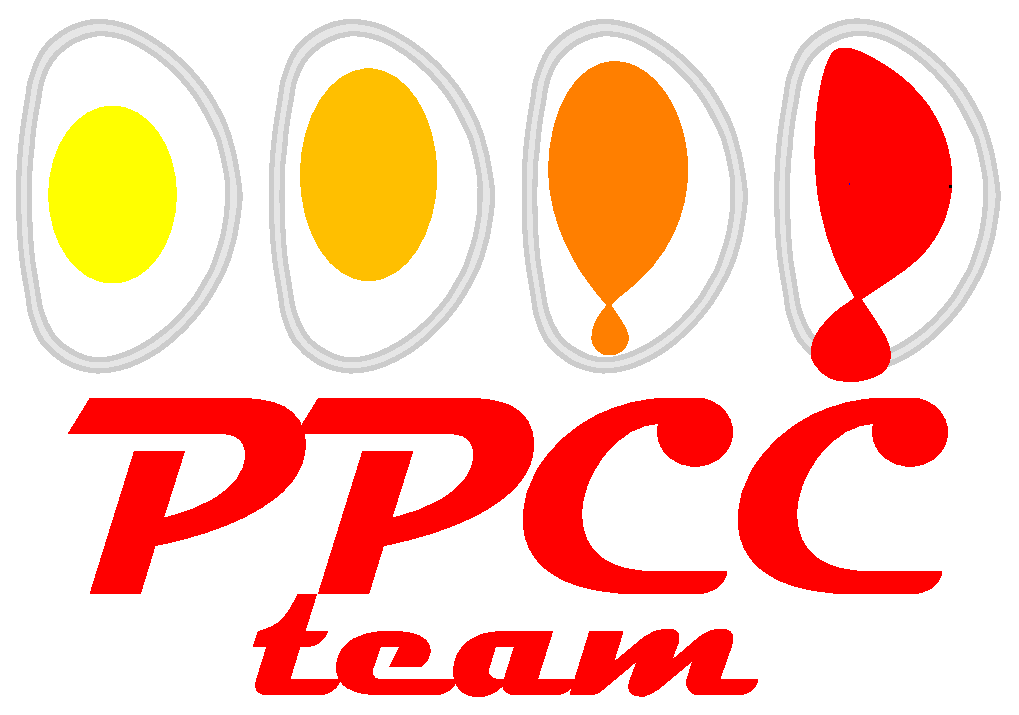
\includegraphics[width=30mm]{PPCClogoRed.eps}
  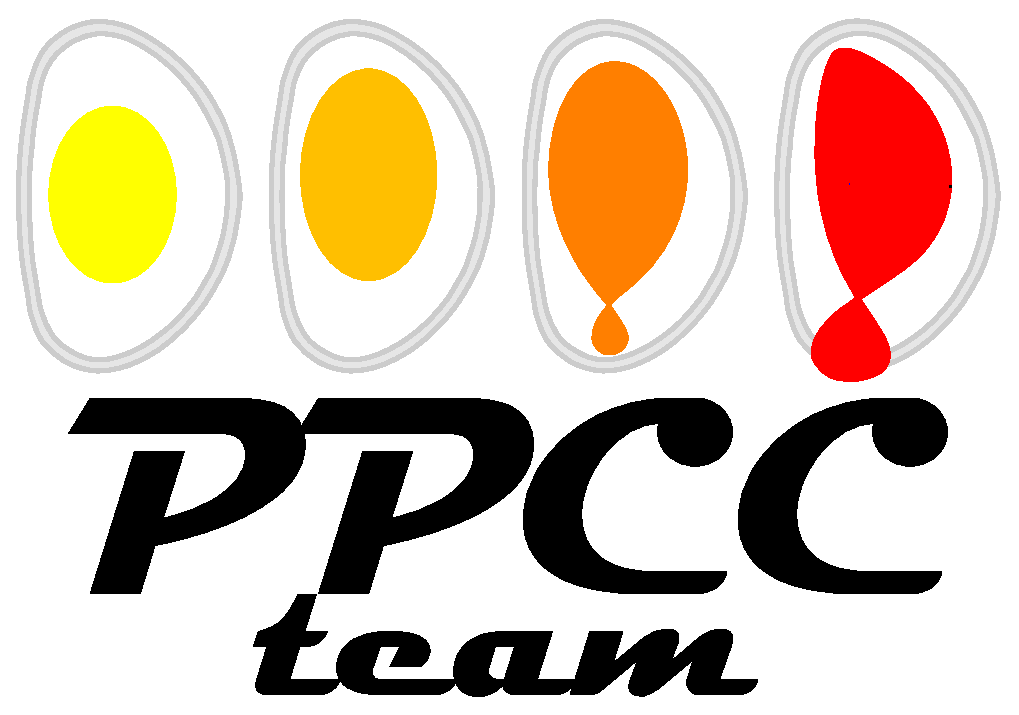
\includegraphics[width=30mm]{PPCClogoBlack.eps}
 \end{center}

\end{titlepage}

\cleardoublepage

\tableofcontents

\listoffigures

\listoftables

\part{Welcome}
\chapter*{Introduction}
\chaptermark{Introduction}



% introduzione in cui parliamo di BaseLib/MARTe in modo generale
% presentiamo lo schema logico dopo di che spieghiamo brevemente ogni singola componente

% BaseLib/MARTe �
% software framework, distribuito, component based, supporta diverse arch, diversi OS
BaseLib/MARTe are togheter a complete software framework to run a distributed control code on different architectures and operating systems. BaseLib/MARTe are not only a middleware but include also a collection of different components, i.e. computational blocks. \\

% BaseLib/MARTe �
% rapid design (se ci sono i componenti), fast time to market
A control system is not more than the interconnection of computational blocks, devices that read signals from the environment and then write them out of the digital system. If a digital control system can be completely designed with blocks included in the BaseLib/MARTe library the implementation is straightforward and can require only a couple of hours. \\

% Differenza tra BaseLib e MARTe
The whole project can be logically splitted in BaseLib, MARTe and the components collection. BaseLib offers the basic data structures, an architecture and OS independent API, an object accounting and tracing infrastructure, a serialization and reflection faciliy and all key mechanisms to run a control system; MARTe lets the control algorithm run.

The componets collection is a growing set of algorithmic blocks (GAMs), device drivers adaption blocks (IOGAMs) and device drivers (GACQMs). All the code is written in C/C++. Figure \ref{f:intro:BaseLibMARTe} is a complete schema of the software framework we are going to analyse in this text. \\

\begin{figure}[h!]
 \begin{center}
  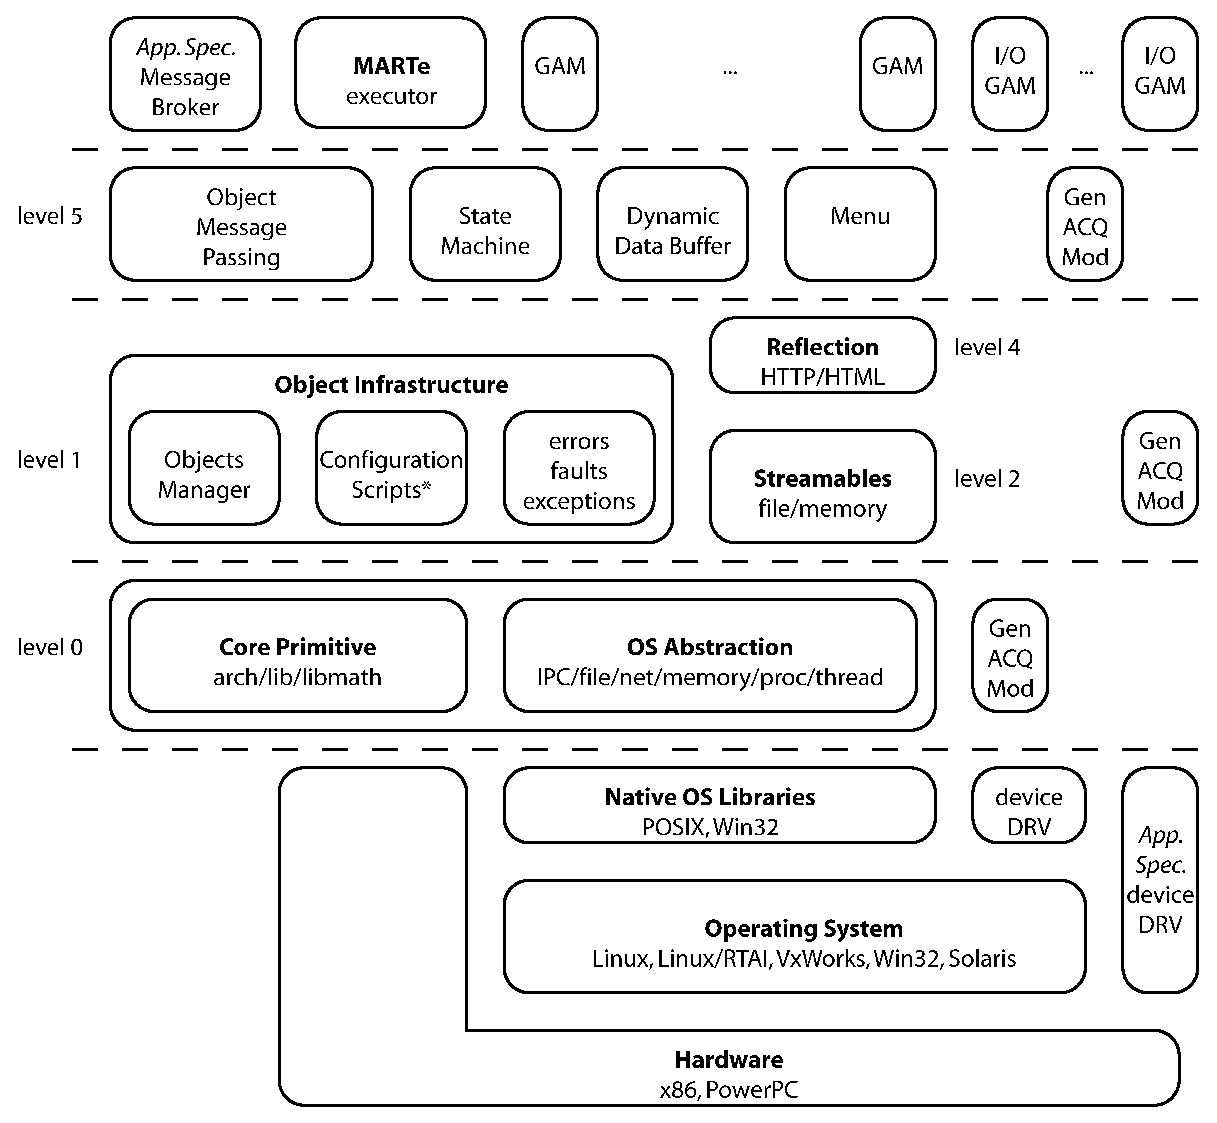
\includegraphics[width=0.63\textwidth]{images/BaseLibMARTe1.eps}
  \caption{BaseLib and MARTe schema}
  \label{f:intro:BaseLibMARTe}
 \end{center}
\end{figure}

The cited Figure highlights the supported operating systems, those are: Microsoft Windows$^\copyright$ 32bit, Linux, Linux/RTAI, Wind River VxWorks$^\copyright$ and Sun Microsystems Solaris$^\copyright$. The supported architectures are: Intel x86 and IBM/Motorola PowerPC (now Freescale), BaseLib/MARTe worked also on SPARC machines but it is not recently tested on. A list of supported I/O and timing devices (ADC and DAC boards) is not available yet. \\


% Posizioniamo BaseLib/MARTe tra i software di controllo come OROCOS
BaseLib/MARTe is a rapid deve lopment control software that can be suitable to automation industry, robot control and manufaturing processes supervision. In those markets we can find other software products, never used in fusion research, those softwares comes from differents experience but most of them lead to the same functionalities and ideas on which BaseLib/MARTe was built. \\

The oldest project we can find on Internet is \textbf{OSACA} (http://www.osaca.org), i.e. Open System Architecture for Controls within Automation systems, focuses on industrial control, is not opensource and probably not manteined yet. There are two government founded project: \textbf{TORERO}, TOtal life cycle web-integrated control design architecture and methodology for distributed control systems in factory automation (http://www.uni-magdeburg.de/iaf/cvs/torero/), and \textbf{OMAC}, the Open Modular Architecture Controller (http://www.isd.mel.nist.gov/projects/). Fully open source university founded projects are: \textbf{OROCOS} (http://www.orocos.org) the Open RObot COntrol Software; \textbf{MCA2} (http://www.mca2.org/) the Modular Controller Architecture (Version 2); \textbf{MICROB} (http://www.robotique.ireq.ca/microb/en/index.html) the Modules Int\'egr\'es pour le Contr\^ole de ROBots and \textbf{OASYS} (http://www-lar.deis.unibo.it/oasys/) the Open source software for industrial Automation and distributed SYstemS (probably part of the TORERO alliance). \\

% saerebbe da spiegare meglio perche
% fondamentalmente perche non e a componenti ma soprattutto e un middleware
The famous \textbf{EPICS} framework (the TANGO framework can be considered as well) doesn't appear in the previous list because it doesn't provide all the basic architectural and design requirement a generic control systems needs to be setup. EPICS, as well as \textbf{CORBA} in the Enterprise Market, is a middleware: it just defines a common protocol to lets different machines (equipped with potentially different OS and processor) communicate. Another middleware used by many automation companies on only Microsoft enabled products is \textbf{OPC} (http://www.opcfoundation.org) the OLE for Process Control, it exploits Microsoft's OLE/COM/DCOM technologies. \\

Various instances of BaseLib/MARTe running in a distributed system can communicate using object messaging, application specific message brokers can also be written to handle 3rd party messages (Figure \ref{f:intro:BaseLibMARTe}). There is an ongoing effort to turn BaseLib/MARTe in an EPICS enabled product. \\



\subsection{Project Organization}
% visione generale del progetto dal punto di vista dello sviluppatore
% diverse entita di codice necessarie i.e. project structure (in future: how to compile)
The whole project is structured in at minimum three packages (directories):
\begin{itemize}
 \item MakeDefaults
 \item BaseLib (or BaseLib2)
 \item MARTe
\end{itemize}

Components (i.e. GAMs) are allotted between the \textit{BaseLib} directory and the \textit{MARTe} directory, other GAMs's directory can be present in your project. The directory \textit{MakeDefaults} group togheter all files to build the software, it supports the Microsoft build system as well as the GNU Makefile utility. The directory \textit{BaseLib} holds all BaseLib files and subdirectories, obviously the directory \textit{MARTe} contains all MARTe files and subdirs, that are presented at the end of the chapter. \\

% il sistema e facile da compilare
% perche tutto il codice lo sviluppiamo noi e non richiede librerie esterne
This directories represent the whole software framework, no external library or software is required, only a working supported Operating System. This means no external dependencies, no dependecies checking and a faster time to a ready to use system. Other projects use differents 3d party libraries and its a pain for a user to put all libraries working togheter.
% in futuro si potrebbero usare librerie esterne 
% la via corretta sarebbe come fa insight che viene distribuito con le librerie che sono state usate
The best solution in this sense is to distribuite the 3d party libraries togheter with the software package, this option can be considered in the future to speed up upgrades of the BaseLib/MARTe code (imagine to add XML support). \\

% si puo mettere qualche numero riguardo al numero di classi e interfaccie presenti rispetto al
% numero di classi che ci sono in altri framework a componenti

To compile the whole project two steps are needed: first you must compile BaseLib and then it is possible to build MARTe. When the libraries are ready you need a configuration file to see something running.



\subsection{Component Object Model}
% component object model similarita con altri progetti (OROCOS) [COM, Java]
% patterns, che design patterns sono stati utilizzati
Most software products nowadays utilize several design patterns; BaseLib/MARTe explicitly uses the Container (Composite), the Iterator, Command and State design patterns (last threes of these are considered by the GAMMA behavioral patterns). Also the Observer, Prototype, Adapter, Bridge and Decorator design patterns are used but the implementation comes naturally, without any previous class's design.

% component object model - component oriented programming
% si � puntato sullo sviluppo COM cioe via interfaccia
Instead, the development of BaseLib/MARTe was done following the Component Oriented Programming practice (well known as Component Object Model). Following such paradigm all communications between objects use a well known interface, the source code is infact rich of interface definitions. \\

% component oriented programming - connection oriented programming (GAM)
% di solito un singolo comoponente = un obj --> GAM
BaseLib/MARTe is built on different components, these usually lead to be developed in single classes, i.e. one component is implemented within one C++ class. These is especially true for the computational blocks that realize a control system from an algorithmic point of view.
A control system can be first designed using a Block Diagram Modeller IDE (Matlab Simulink$^\copyright$, Scicos, NI LabView$^\copyright$ or Ptolemy/Kepler) and then converted for execution in BaseLib/MARTe. Each computational block of the diagram will be mapped to a software component called Generic Application Module (GAM); GAMs are then connected via a memory bus component that offers some interfaces but also requires to be compliant to other interfaces. The definition of incoming and outcoming interfaces is usually referred to Connection Oriented Programming and is a particular programming style that is especially useful when aiming for Component Oriented Programming. Figure \ref{f:intro:GAMComponent} show how connection can be setup between components.

\begin{figure}[h!]
 \begin{center}
  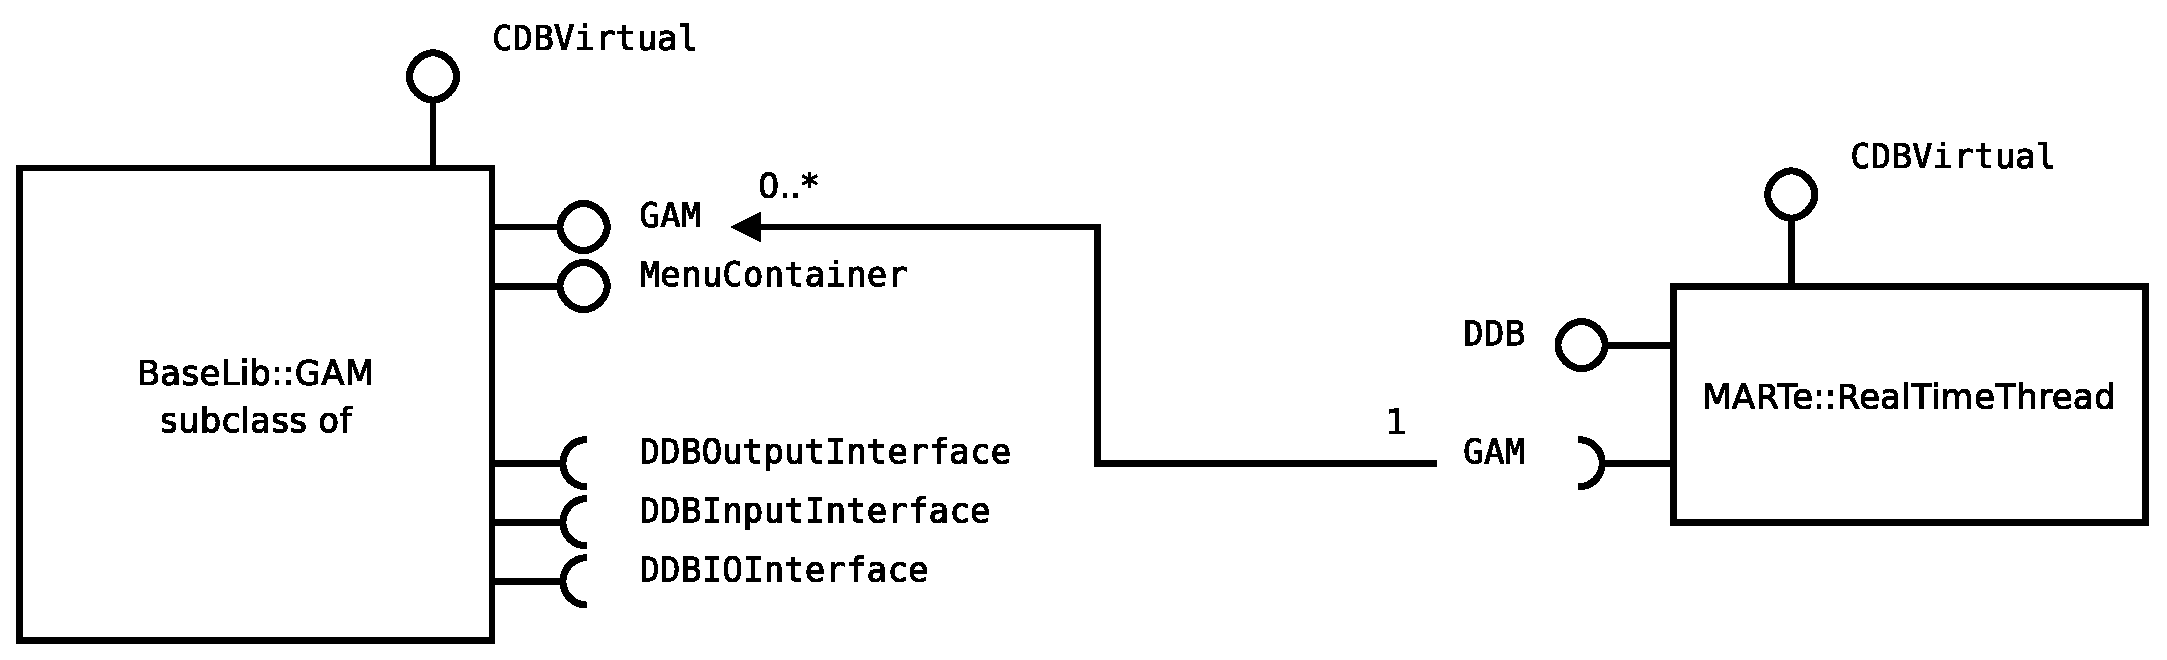
\includegraphics[width=0.77\textwidth]{images/GAMComponent.eps}
  \caption{Components connections in BaseLib/MARTe}
  \label{f:intro:GAMComponent}
 \end{center}
\end{figure}

Such Figure points out the connection between a \texttt{MARTe::RealTimeThread} component and many \texttt{BaseLib::GAM} subclass components, note the multiplicities at each ends of the association.
A \texttt{BaseLib::GAM} subclass component, or simply a GAM, holds receptacles for \texttt{DDBInputInterface}, \texttt{DDBOutputInterface} and \texttt{DDBIOInterface}. Such interfaces lets
a GAM produce and consume datas on the common memory bus called Dynamic Data Buffer (DDB). The \texttt{CDBVirtual} interface lets components load and save its configuration from and to a configuration file (in a human readable format). The \texttt{MenuContainer} interface lets components export a menu user interface to enable users to see and change component's parameter in real time. \\


% i componenti mono source sono le GAM - il resto del codice segue la programmazione OO
% e i componenti non sono esplicitamente definiti
Most of the code in the project that doesn't extends or doesn't implement a GAM is infrastructural and lets GAMs load, connect between them, run and save is state (persistence), the exception is MARTe that is a scheduling entity of all GAMs. Figure \ref{f:intro:BaseLibMARTe3D} illustrate this concept. Note that this doesn't mean that only GAMs are components, all the software is structured using the Component Object Model. \\

\begin{figure}[h!]
 \begin{center}
  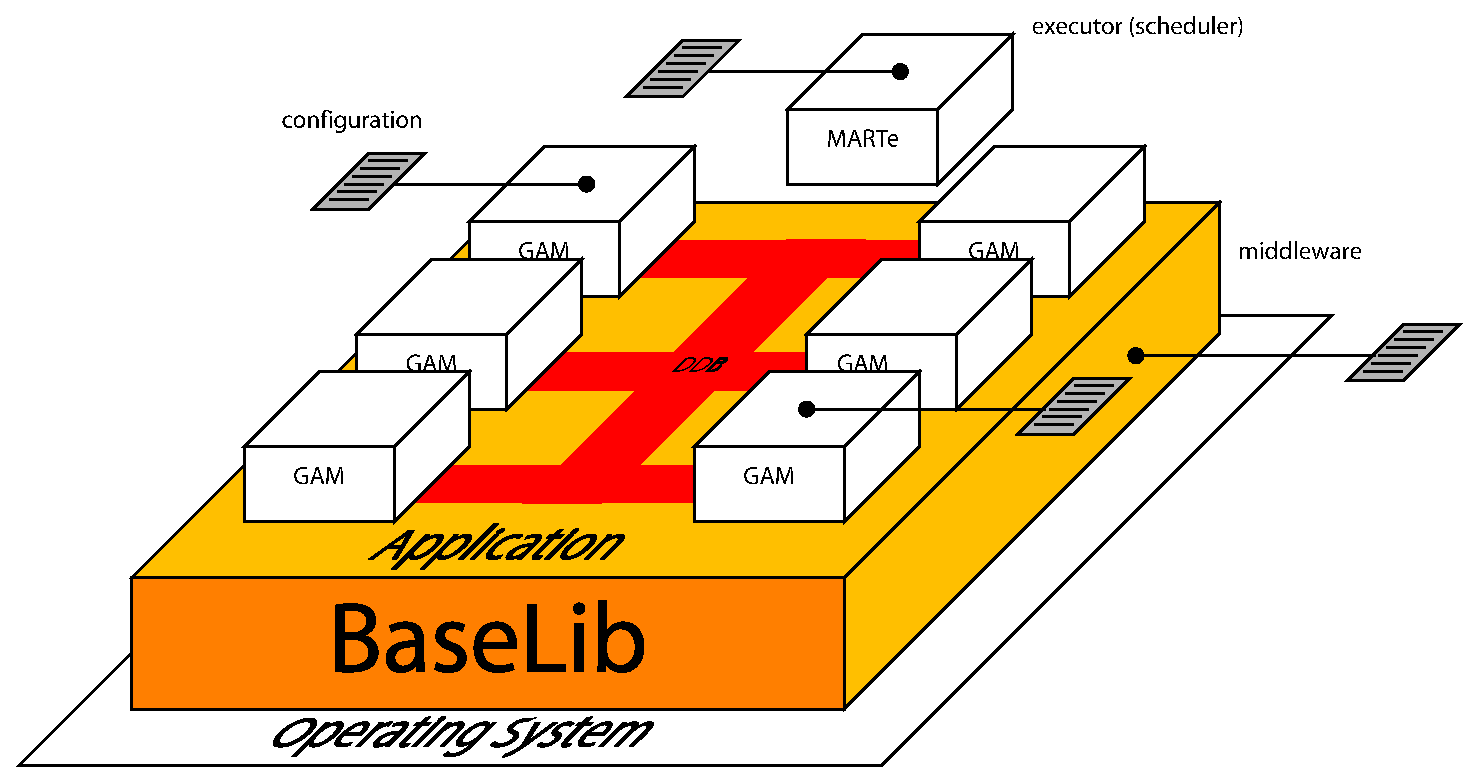
\includegraphics[width=0.77\textwidth]{images/BaseLibMARTe3D.eps}
  \caption{BaseLib and MARTe schema in 3D}
  \label{f:intro:BaseLibMARTe3D}
 \end{center}
\end{figure}

Referring to the same picture is simple to understand what a user application running in BaseLib/MARTe is: \textbf{a collection of interconnected components initialised via a configuration file}. \\

If components for your control system application are just written no understanding of the entire software framework is needed and also no programming skills are required because you can implement the control system using only a human readable/writable configuration file (similar to the Microsoft's \texttt{ini} files). \\



\subsection{Reflection, Persistence, Garbage Collection and Messages}

A big difference between the most used C object oriented version (C++) and the Sun Object Oriented language Java is the lack of reflection, persistence (serialization) and garbage collection of the former.
These capabilities enable Java to manage every aspect of objects lifecycle, from the creation to the destruction providing also a runtime inspection. Both C++ and Java supply runtime introspection (C++ by means of RTTI). \\


Smalltalk and Objective C languages have built-in reflection besides introspection; such languages add Object Messaging. To get an object to do something, you send it a message telling it to apply a method or to do an activity. Programming by messages instead using method calls ensure inter-thread communication safety without holding locks. \\


BaseLib/MARTe as a C/C++ framework supplies to the user a complete solution that introduce in C/C++ language an esay to use reflection, persistence, garbage collection and object messaging, all those capability work on different compilers and different operating systems.
Looking back at Figure \ref{f:intro:BaseLibMARTe} there is a block named \textit{Object Infrastructure}, this block is deepened in Figure \ref{f:intro:BaseLibOI} and implements the core functionalities for object handling and inspection.
Those object level features are not common to a component based software that usually takes into account component-alike properties (this is the behavior of the previous cited OROCOS control framework). Such added capabilities add at minimum another level of complexities to the schema in Figure \ref{f:intro:BaseLibMARTe3D} where for example there is no object message loop. \\

\begin{figure}[h!]
 \begin{center}
  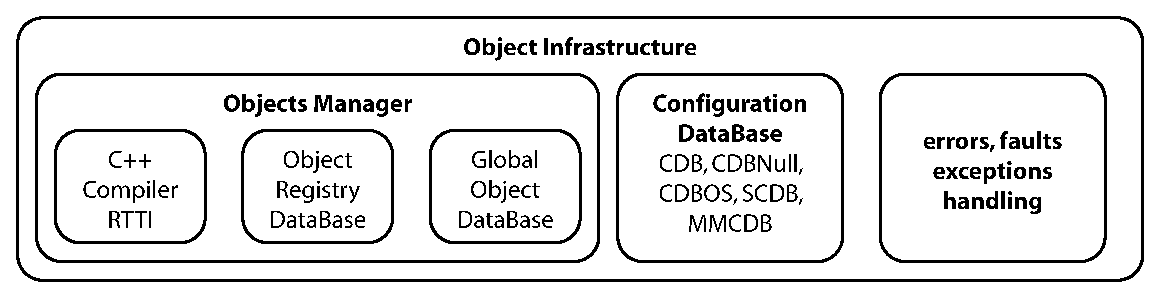
\includegraphics[width=0.77\textwidth]{images/BaseLibOI.eps}
  \caption{BaseLib Object Infrastructure}
  \label{f:intro:BaseLibOI}
 \end{center}
\end{figure}

Figure \ref{f:intro:BaseLibOI} highlights the different entity componing the \textit{Object Infrastructure}: an object manager built on top of the C++'s compiler RTTI, an Object Registry DataBase (ORDB), i.e. a list of all objects type currently loaded in the system; a Global Object DataBase (GODB), i.e. a list of all currently instantiated objects; a configuration utility (the CDB) that lets load and save object's attributes (i.e. implement the serialization) and an error management unit. \\

% come si arriva alla serializzazione
% late binding implicito
Exploiting the RTTI facility and language macros the ORDB and the GODB implement reflection and garbage collection. Garbage collection is done by refernce counting. External live reflection capability is offered via an HTTP server at highers level (many industrial boards nowadays lets the user inspect it via a web browser).

The CDB exploiting ORDB and GODB adds serialization. The serialization in BaseLib/MARTe is done by each object, i.e. only the single object is aware of its attributes (or parameters). The serialization is not done on human unreadable format but in a simple format that lets a user write it's own file, a configuration file is a human readable serialization of objects. A whole control system can be written using only a single configuration file without a single line of C/C++.

% object messaging
Object Messaging is achieved by the \textit{Object Message Passing} infrastructure in a higher level of the framework (have a look at Figure \ref{f:intro:BaseLibMARTe}). This entity will be integrated in the Object Infrastructure. \\



%\subsubsection{Code Conventions}
% scelte implementative del codice
% classi inline, problema delle DLL
% le classi vengono scritte con il codice in C per permettere alle DLL di essere compilate in modo che si possa fare un late binding
% il motivo in realta per il momento mi e oscuro. cmq o centra con le DLL oppure centra con il supporto a diversi compilatori.
% in pratica molte classi hanno i loro metodi implementati come inline che richiamano funzioni C friend
% invece di avere comuni metodi implementati nel file cpp con la dichiarazione classe::nome



% BaseLib states
% BaseLib organization (current version)
\section{BaseLib}
BaseLib is a library, i.e. a collection of codes. BaseLib relay on very few global data structures loaded at initialization time, it is the user that loads the framework via a function call that invoke all the startup process.

The startup process (CREATION state) of BaseLib reads a configuration file (also in memory) then creates all objects in such file with the correct attribute's values (exploiting serialization). If the creation finishes without any problem the framework is in the RUNTIME state, in this state MARTe is running. If MARTe chooses to exit move all the system in the DELETION state, the last state before application end. In each state BaseLib can moves to the ERROR state. The whole BaseLib state transitions are depicted in Figure \ref{f:intro:BaseLibStates}; BaseLib doesn't know about its internal state unless it is in ERROR, BaseLib' states are just an abstraction to understand its behaviour. \\

\begin{figure}[h!]
 \begin{center}
  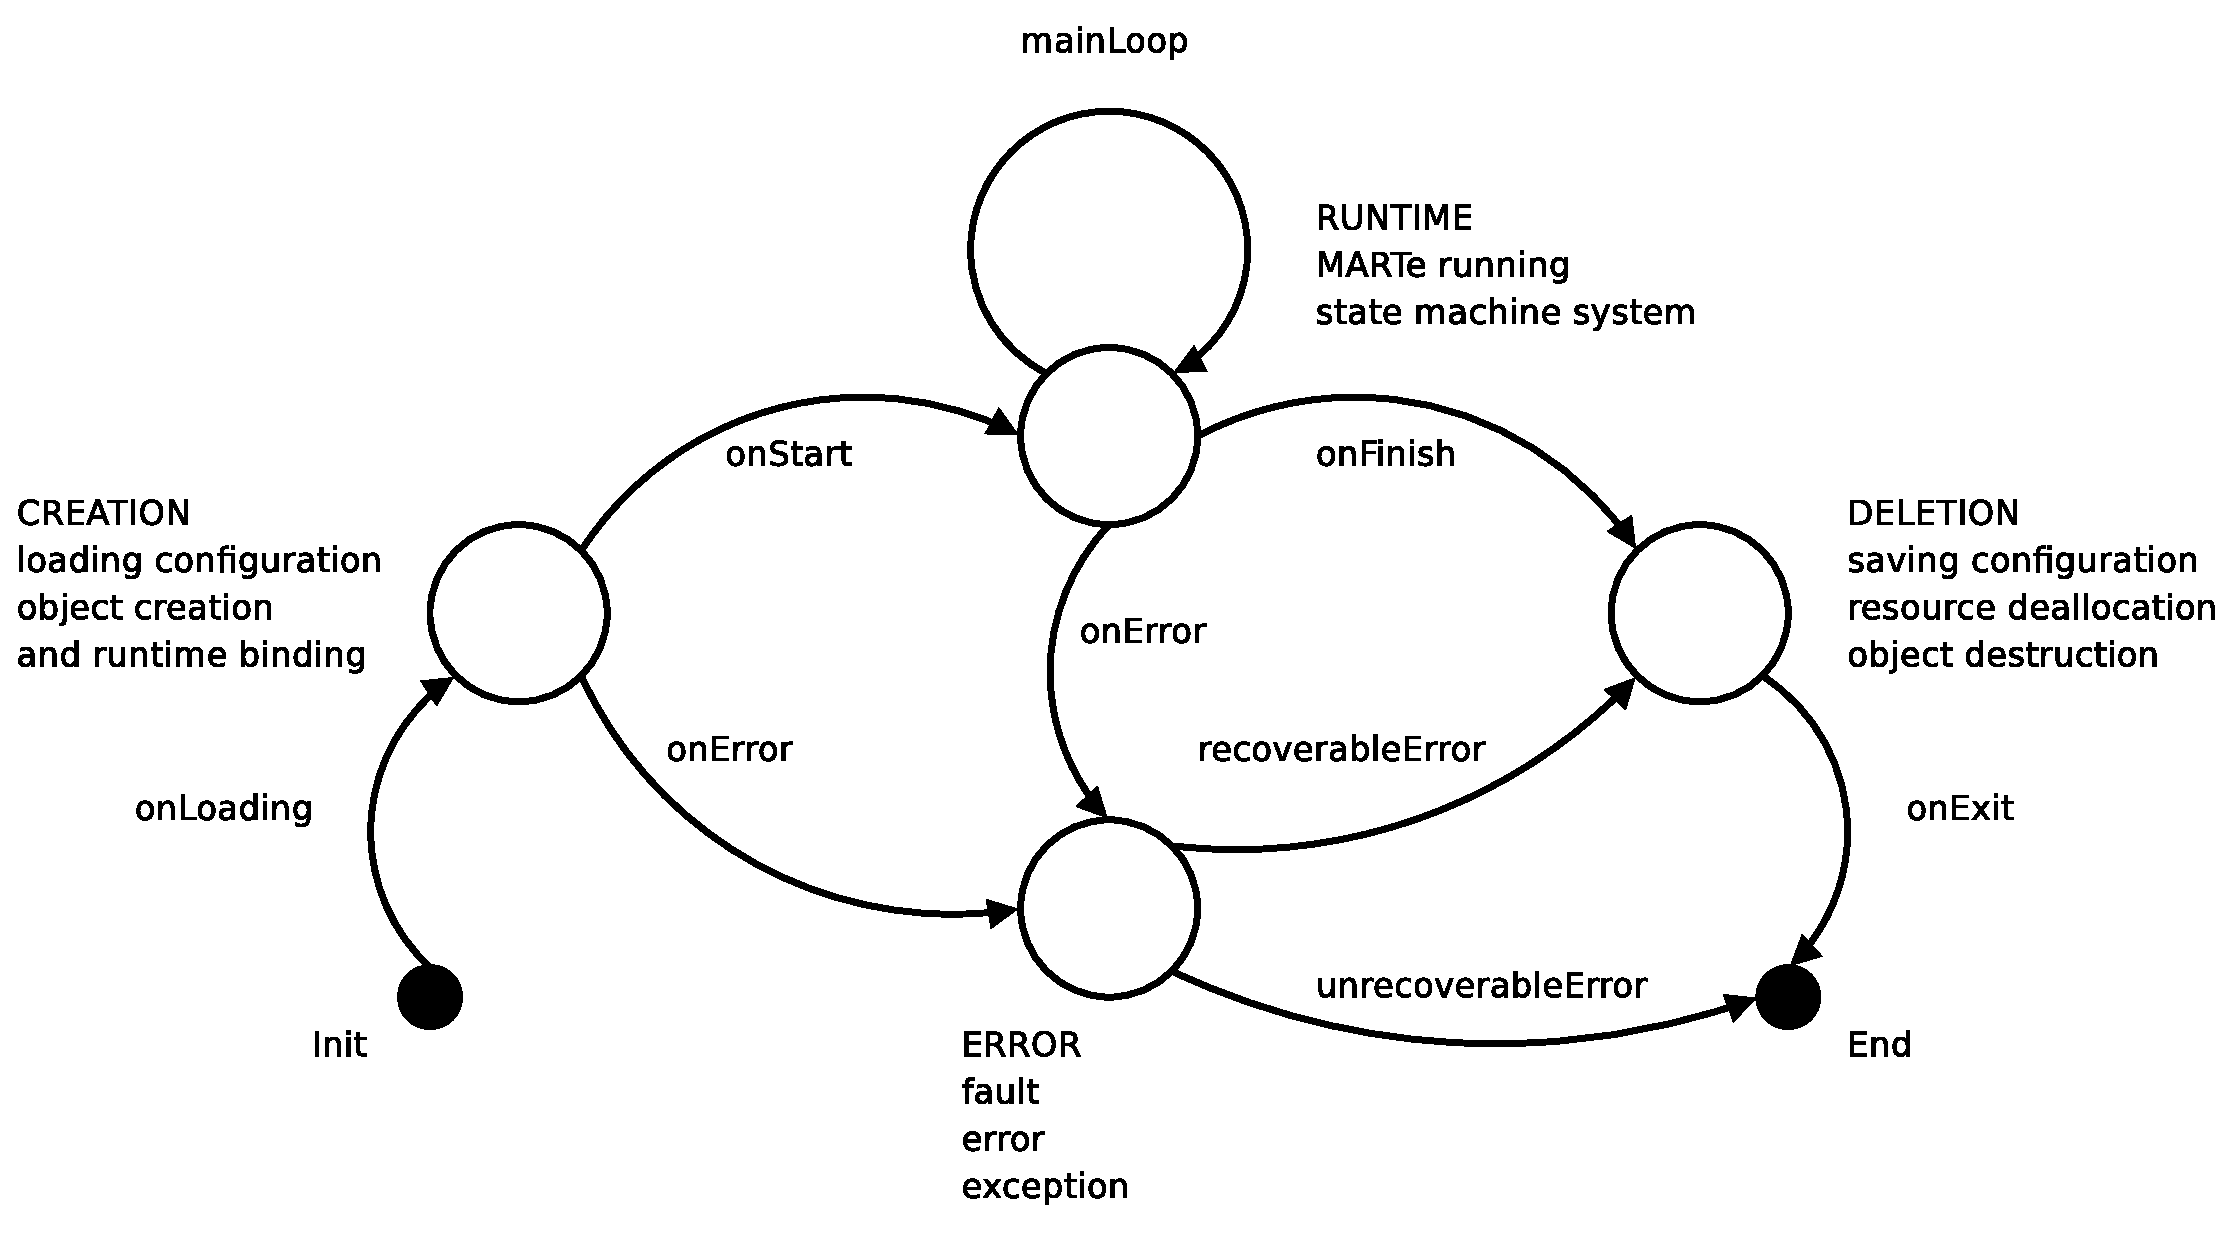
\includegraphics[width=0.77\textwidth]{images/BaseLibStates.eps}
  \caption{BaseLib's main states}
  \label{f:intro:BaseLibStates}
 \end{center}
\end{figure}

BaseLib's core source code is partitioned right now in seven different directories, each one is a \textit{level} starting from \textit{level0} up to \textit{level6}. Code in a directory within an higher \textit{level} depends on code in low \textit{level} directories like in an hierarchy relationship.

BaseLib contains also other code, it holds a collection of GAMs (common and wide used ones), some testing applications and useful debugging and logging tools. All that in four different directories: \textit{LoggerService}, \textit{GAMs}, \textit{BaseLibTests}, \textit{BaseLibTools}.

In this work only \textit{level} directories will be analised. At the end of reading it will be easy to understand that the subdivision by compilation dependence doesn't ease the understanding of the project (also if can be a good choice for debugging the project). Table \ref{T:levels} summarizes which component it is possible to find in each level. The CDB's code for example is spreaded between \textit{level0}, \textit{level1}, \textit{level3} and \textit{level6}. Same work must be done in these direction to ease code comprehension and modularity. \\

\begin{table}[!ht]
 \begin{center}
  \begin{tabular}{|l|l|}
\hline
\textbf{level 0} & OS Abstraction\\
 & Core Primitives \\
\hline
\textbf{level 1} & Garbage Collection \\
 & ObjectRegistryDataBase (ORDB) \\
 & GlobalObjectDataBase (GODB) \\
 & ConfigurationDataBase (CDB) \\
\hline
\textbf{level 2} & streams \\
 & ConfigurationDataBase (CDB) \\
\hline
\textbf{level 3} & ConfigurationDataBase (CDB) \\
 & ConfigurationDataBase OutputStream (CDBOS) \\
 & parser \\
\hline
\textbf{level 4} & HTTP, HTML protocol libraries\\
\hline
\textbf{level 5} & Dynamic Data Buffer (DDB)\\
 & Generic Acquisition Module (GAM) \\
 & Messages \\
 & State Machine \\
 & Menu \\
\hline
\textbf{level 6} & Memory Mapped CDB (MMCDB)\\
 & maths objects \\
\hline
  \end{tabular}
 \caption{BaseLib levels}
 \label{T:levels}
 \end{center}
\end{table}


% MARTe states
% MARTe organization (current version)
\section{MARTe}
MARTe library is a collection of GAMs, IOGAMs, GACQMs and an executor (or dispatcher). Such executor is a thread that run consecutively a set of GAMs and IOGAMs; the set that is currently running depends on the state of the plant system and the controller machine. There are basically four sets: \textit{initialising}, \textit{offline}, \textit{online} and \textit{safety}. In Figure \ref{f:intro:MARTeStates} the states of the plant system are depicted; usually the \textit{initialising} set is executed only during the INIT state, the \textit{online} set is executed during PREPULSE, PULSE and POSTPULSE; \textit{offline} set is executed in IDLE and WAITINGPRE states. When some error occurs the currently running set is substitued with the \textit{safety} set. \\

\begin{figure}[h!]
 \begin{center}
  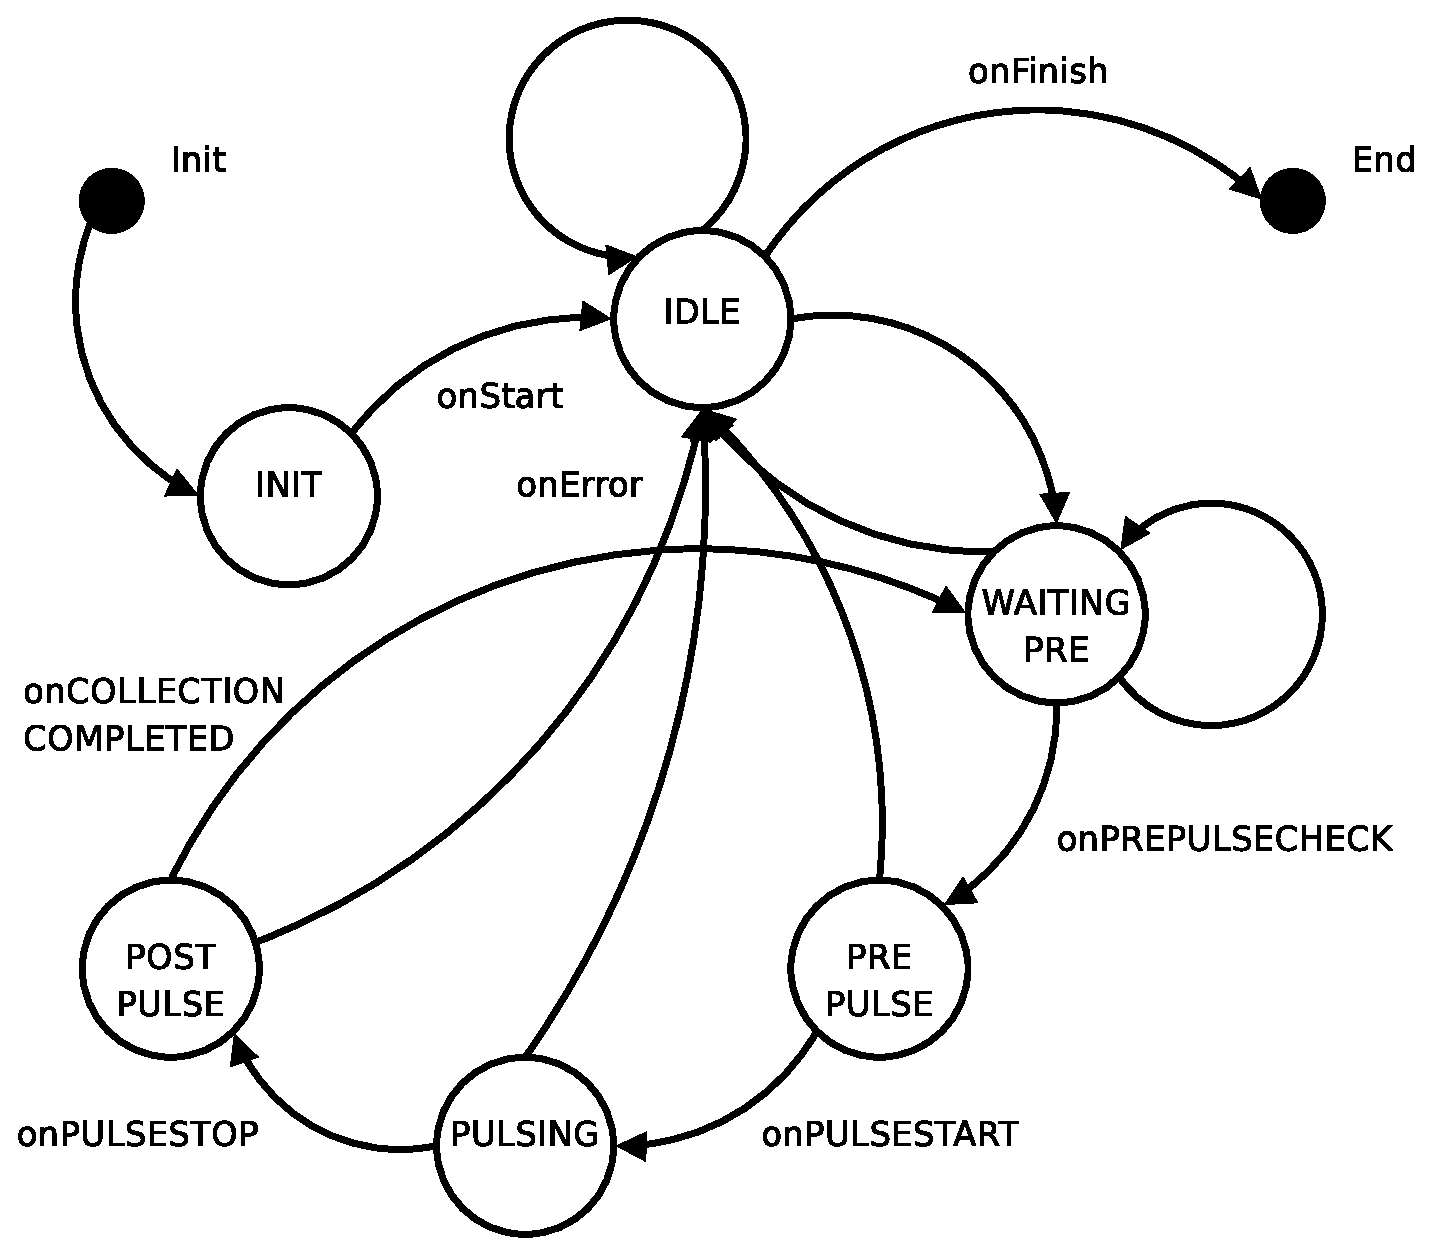
\includegraphics[width=0.50\textwidth]{images/MARTeStates.eps}
  \caption{MARTe States}
  \label{f:intro:MARTeStates}
 \end{center}
\end{figure}

MARTe originates as the first application built on BaseLib library. Some components, like the \textit{RealTime Thread} (the executor), were added because not in BaseLib, MARTe is also the configuration file that request the instantiation of a precise set of components. Figure \ref{f:intro:MARTe} depict the different componets MARTe require to be instantiated.

\begin{figure}[h!]
 \begin{center}
  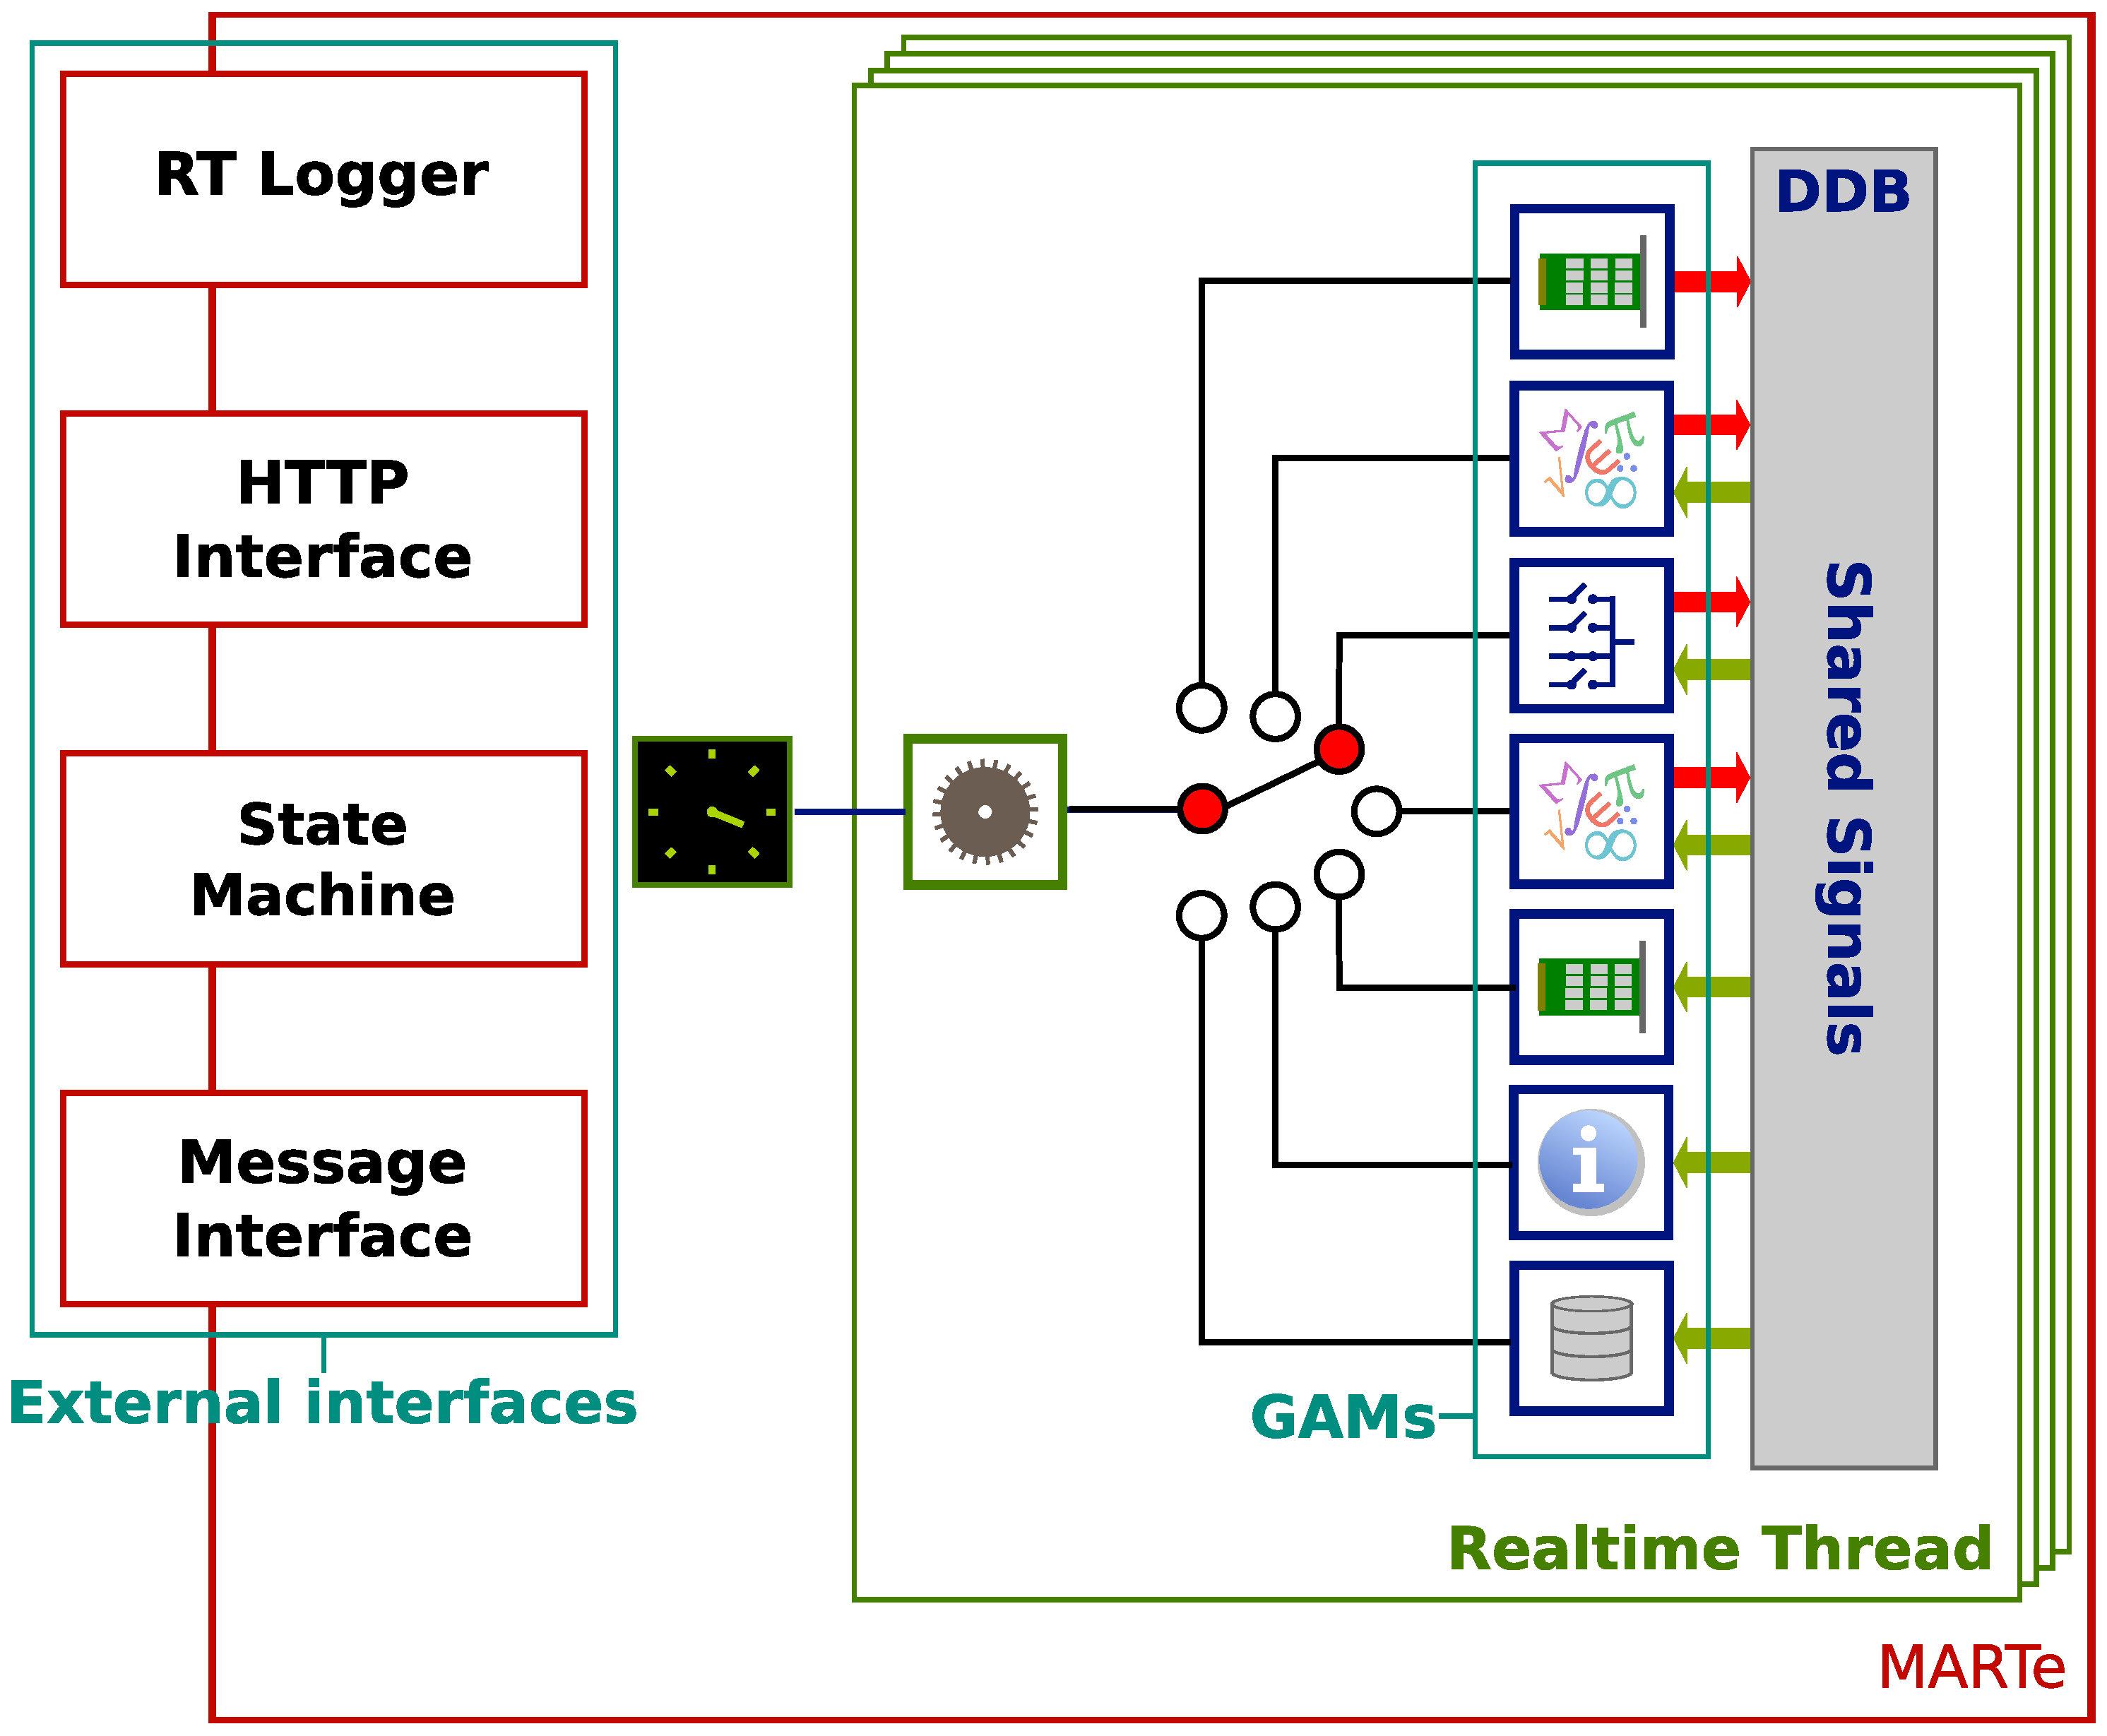
\includegraphics[width=0.48\textwidth]{images/MARTeComponents.eps}
  \caption{MARTe Components}
  \label{f:intro:MARTe}
 \end{center}
\end{figure}

In such Figure there are at least three different components that come from BaseLib: the \textit{HTTP server}, the \textit{Messaging} infrastructure and an \textit{external state machine} that communicate with the internal one. In the Figure is not depicted the communication library that connects MARTe to plant system rendering the application a part of the whole distributed system. The communication library is included in MARTe, right now there is only CODASLib that supports the JET communication protocol; forthcoming libraries will be MDSplusLib and EPICSLib.

\begin{table}[!ht]
 \begin{center}
  \begin{tabular}{|l|l|}
\hline
 \textbf{MARTeSupportLib} & \\
\hline
 \textbf{GAMs} & EventCollection, WaveformCollection, DataCollection \\
 & WebStatistics, Statistics \\
 & Hysteresis, Noise, CurrentControl \\
\hline
 \textbf{IOGAMs} & ATCA, MPV956, MPV922 \\
 & ForeHE, Interphase, LinuxSocket (UNIX), WinSock \\
 & WinTimer, LinuxTimer (UNIX), VxWorksTimer, HRT \\
\hline
 \textbf{CODASLib} & \\
 \textbf{MDSplusLib}* & \\
 \textbf{EPICSLib}* & \\
\hline
  \end{tabular}
 \caption{MARTe directory tree}
 \label{T:trees}
 \end{center}
\end{table}


\section{Remarks}
TODO\\




\part{BaseLib}
\chapter{BaseLib Level 0}
\chaptermark{Level 0}



BaseLib Level0 is a mixture of different classes that must provide the developer with a complete system abstraction. In fact such abstraction stops at the operating system level without offering device driver's API. Each device driver must be developed separately for a specific architecture and OS. \\

To better understand what services there are in BaseLib Level 0 the following argomentation subdivid it in a logical way extrapolating these sections:

\begin{itemize}
 \item Architectures
 \item Lists

 \item IPC

 \item Network
 \item Files, Streams

 \item Errors, Exceptions
 \item Memory
 \item Processes, Threads

 \item Mathematic
\end{itemize}

BaseLib2 was already ported to the following OS: OS/2$^{\copyright}$, VxWorks$^{\copyright}$, Linux, Linux/RTAI, Solaris$^\copyright$ and MS Windows$^\copyright$.






\section{Architectures}
\begin{figure}[h!]
 \begin{center}
  \includegraphics[width=\textwidth]{level0/level0-arch.eps}
  \caption{BaseLib Level0 Architecture classes}
  \label{f:level0:arch}
 \end{center}
\end{figure}

This group of classes (Figure \ref{f:level0:arch}) adds the very low level support to the library, addressing architecture and hardware support, i.e. processor assembly instructions and special processor register functions.
The Architecture group include the following classes:
\begin{itemize}
 \item Processor
 \item ProcessorType

 \item LoadableLibrary
 \item RTAILoader

 \item Atomic
 \item SPAtomic

 \item HRT (High Resolution Timer) 
 \item TimeoutType
 \item Sleep
\end{itemize}



\subsubsection{Processor}
\texttt{[Processor.h, Processor.cpp]}\\
The Processor class lets you discover how many processor there are on the machine and which kind of processor are and it's characteristics like the clock and the family name.

\begin{lstlisting}[
extendedchars=true,%
basicstyle=\fontfamily{pcr}\fontseries{m}\selectfont\footnotesize, %
stepnumber=1,%
numberstyle=\tiny,%
keywordstyle=\footnotesize\tt ,%
language=C++]
public:
   static uint64 ClockFrequency();
   static double ClockPeriod();

   static const char *Name();
   static uint32 Family();
   static uint32 Characteristic(uint32 capId);

   static int32 Available();
   static void ReScanCPU();
\end{lstlisting}

All methods are static; \texttt{ClockFrequency} return the CPU or the HRT frequency, \texttt{ClockPeriod} return the CPU period (the inverse of the frequency). \texttt{Name} return the processor name or type, \texttt{Family} return the brand of the processor, \texttt{Characteristic} return some capabilities of the CPU, \texttt{Available} return the number of available cpus on the system.
Th function \texttt{ReScanCPU} reinitialize the static processor object and redo a scan of the system to count the number of CPU.\\


In \textit{Processor.cpp} there is also a \texttt{HRTCalibrator} class that calibrate the CPU clock. Such class has only a constructor and no other methods or attributes. The \texttt{HRTCalibrator} class is statically instantiated with the name \texttt{hrtCalibrator}; it just sets some global variables at the start up executing the code in its contructor. \\



\subsubsection{ProcessorType}
\texttt{[ProcessorType.h]}\\
The \texttt{ProcessorType} class defines the processors where a particular task should run. There is a unique mask argument as a \texttt{uint32}, the \texttt{processorMask}, this is a bitmask and allow the maximum presence of 32 CPU on a system.
The interface let the user initialize the class with a bitmask and adding CPUs but never remove one or more. There are some operator overlaoding.


For example, if we have a task is that will run on cpu 2 and 3 the mask is: 0x06 (00000110).


\begin{lstlisting}[
extendedchars=true,%
basicstyle=\fontfamily{pcr}\fontseries{m}\selectfont\footnotesize, %
stepnumber=1,%
numberstyle=\tiny,%
keywordstyle=\footnotesize\tt ,%
language=C++]
public:
   uint32 processorMask;

   ProcessorType(const uint32 cpuMask = 0xFE);
   ProcessorType(const ProcessorType &pt);

   void SetMask(const uint32 mask);
   void AddCPU(const uint32 cpuNumber);

   void operator=(const uint32 cpuMask);
   void operator=(const ProcessorType &pt);
   void operator|=(const uint32 cpuMask);
   void operator|=(const ProcessorType &pt);
\end{lstlisting}



\subsubsection{LoadableLibrary}
\texttt{[LoadableLibrary.h]}\\
The class \texttt{LoadableLibrary} lets BaseLib, that is a component oriented framework, load its components by means of loading external libraries. On different Operating Systems libraries have different extensions.

\begin{table}[!h]
 \begin{center}
  \begin{tabular}{|l|l|}
   \hline
    GENERAL ACQUISITION MODULE & \texttt{*.gam} \\
    HIGH LEVEL DRIVER & \texttt{*.drv} \\
    STD NAME FOR DLL & \texttt{*.dll} \\
    LINUX NAME FOR DLL & \texttt{*.so} \\
   \hline
   \end{tabular}
   \end{center}
  \caption{Loadable libraries extensions}
 \label{t:extensions}
\end{table}



\subsubsection{Atomic}
\texttt{[Atomic.h, Atomic.cpp]}\\
The class is build up only of static methods. Such routines are performed by the CPU without interruption; these are slower than those in \textit{SPAtomic.h}, but are granted to work on multiprocessor machines.

The Solaris port is quite old and is the only one that is not coded with assembly instructions.

\begin{lstlisting}[
extendedchars=true,%
basicstyle=\fontfamily{pcr}\fontseries{m}\selectfont\footnotesize, %
stepnumber=1,%
numberstyle=\tiny,%
keywordstyle=\footnotesize\tt ,%
language=C++]
public:
   static inline void Increment (volatile int32 *p );
   static inline void Increment (volatile int16 *p);
   static inline void Increment (volatile int8 *p);

   static inline void Decrement (volatile int32 *p);
   static inline void Decrement (volatile int16 *p);
   static inline void Decrement (volatile int8 *p);

   static inline int32 Exchange (volatile int32 *p, int32 v);

   static inline bool TestAndSet(int32 volatile *p);
   static inline bool TestAndSet(int16 volatile *p);
   static inline bool TestAndSet(int8  volatile *p);
\end{lstlisting}

The class offer methods to atomically increment, decrement, exchange (swap) and test and set 8bit, 16bit and 32bit variables, 64bit variables are not supported yet.



\subsubsection{SPAtomic}
\texttt{[SPAtomic.h, SPAtomic.cpp]}\\
Single Processor Atomic operation support. The interface of exported methods is identical to the \texttt{Atomic} class, the only thing that differ is the source code: atomic operations are inherently processor dependent, not all CPU implements atomic instruction in the same way protecting sections to be exectued concurrently.\\ 


This routine are not processor safe, not to be executed in multiprocessor environments. \\


\begin{lstlisting}[
extendedchars=true,%
basicstyle=\fontfamily{pcr}\fontseries{m}\selectfont\footnotesize, %
stepnumber=1,%
numberstyle=\tiny,%
keywordstyle=\footnotesize\tt ,%
language=C++]
public:
    static inline void Increment (volatile int32 *p );
    static inline void Increment (volatile int16 *p);
    static inline void Increment (volatile int8 *p);

    static inline void Decrement (volatile int32 *p);
    static inline void Decrement (volatile int16 *p);
    static inline void Decrement (volatile int8 *p);

    static inline int32 Exchange (volatile int32 *p, int32 v);

    static inline bool TestAndSet(int32 volatile *p);
    static inline bool TestAndSet(int16 volatile *p);
    static inline bool TestAndSet(int8  volatile *p);
\end{lstlisting}



\subsubsection{HRT}
\texttt{[HRT.h, HRT.cpp]}\\
The HRT or High Resolution Timer class exhibit a series of public static methods. Methods let the user query the system High Resolution Timer about the current time count, in machine ticks. In a Pentium class processor the offered methods (\texttt{HRTCounter}, \texttt{HRTCounter32}) are perform a \texttt{rdtsc} assembly instruction respectively returning a 64bit and a 32bit number. The \texttt{rdtsc} x86 assembly instruction read the Time Stamp Counter register of the processor that is a 64bit register present on all x86 processors since the Pentium. It counts the number of ticks since reset.

\begin{lstlisting}[
extendedchars=true,%
basicstyle=\fontfamily{pcr}\fontseries{m}\selectfont\footnotesize, %
stepnumber=1,%
numberstyle=\tiny,%
keywordstyle=\footnotesize\tt ,%
language=C++]
public:
   static inline int64 HRTCounter();
   static inline uint32 HRTCounter32();
\end{lstlisting}

To convert the readed value to a more significant value there are some other methods. The method \texttt{HRTFrequency} return the CPU frequency, \texttt{HRTPeriod} the period of the CPU clock and \texttt{TicksToTime} simply convert CPU ticks in time (seconds).

\begin{lstlisting}[
extendedchars=true,%
basicstyle=\fontfamily{pcr}\fontseries{m}\selectfont\footnotesize, %
stepnumber=1,%
numberstyle=\tiny,%
keywordstyle=\footnotesize\tt ,%
language=C++]
   static inline int64 HRTFrequency();
   static inline double HRTPeriod();
   static inline double TicksToTime(int64 tStop,int64 tStart=0);

   uint32 SystemMsecTime();
\end{lstlisting}

Last method is not static and require an object to be instantiated. Is really strange that this method is static, looking at the implementation it doesn't require object attributes. It count the ms from reset.



\subsection{Design Notes}

HRT's last method must be static. Infact no class methods and attributes are called. The current code follow.

\begin{lstlisting}[
extendedchars=true,%
basicstyle=\fontfamily{pcr}\fontseries{m}\selectfont\footnotesize, %
stepnumber=1,%
numberstyle=\tiny,%
keywordstyle=\footnotesize\tt ,%
language=C++]
uint32 HRTSystemMsecTime(){
   int64 count      =  HRTRead64();
   double msecTime  =  HRTClockCycle() * 1000.0;
   msecTime = msecTime * count;
   return (uint32) msecTime;
}
\end{lstlisting}

\texttt{HRTCalibrator} class must be moved and integrated in \texttt{HRT} class; now it is declared in Processor.cpp, not well designed. \\


ProcessorType class is not scalable. Scalability and modularity are central concepts of Object Oriented Design. It is not a good choice to dress a \texttt{uint32} as a class with only one real method (\texttt{Add}). The first step is to add at least a \texttt{Remove} method. The second step is to extend the \texttt{ProcessorType} class to support a generic number of processors; instead of an uint32 we have to add a bitmap, in this way we can define a set of class that work on bitmaps and support a generic number of processors.\\


Another required extension (that could be handle in a generic way) is the support of atomic operation with generic length variables starting with the 64bit support in the \texttt{Atomic} and \texttt{SPAtomic} classes. \\






\section{Lists}
\begin{figure}[h!]
 \begin{center}
  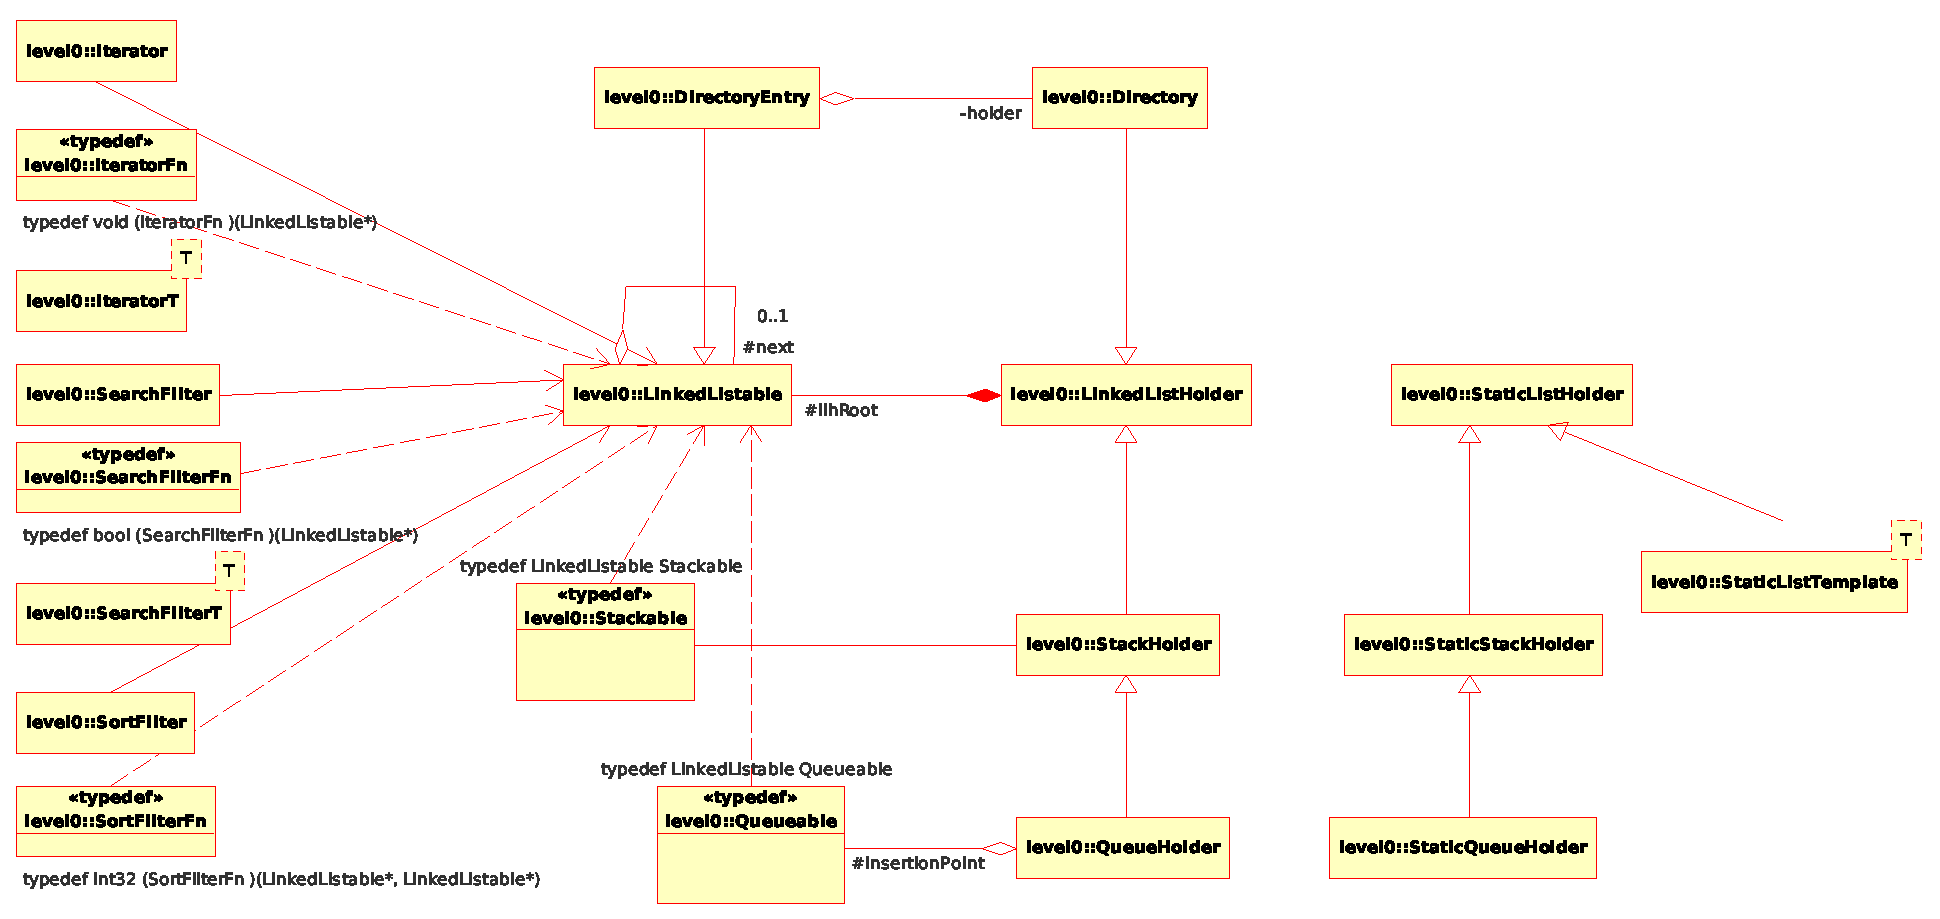
\includegraphics[width=\textwidth]{level0/level0-lists.eps}
  \caption{BaseLib Level0 Lists classes}
  \label{f:level0:lists}
 \end{center}
\end{figure}

The list abstraction is the most used abstraction in BaseLib. On top of a linked list it's build each BaseLib's DataBase; the SemNameDataBase (SNDB), GlobalObjectDataBase (GODB), ObjectRegistryDataBase (ORDB), ConfigurationDataBase (CDB) and many others.

Lists are mainly divided in two categories: linked list and static list. Figure \ref{f:level0:lists} graph all classes involved in this group, those classes can be further splitted in linked and static list and an the \textit{directory} abstraction that is a simple implementation of a single linked list. Static lists are basically vectors.



\subsection{Linked Lists}
\begin{figure}[h!]
 \begin{center}
  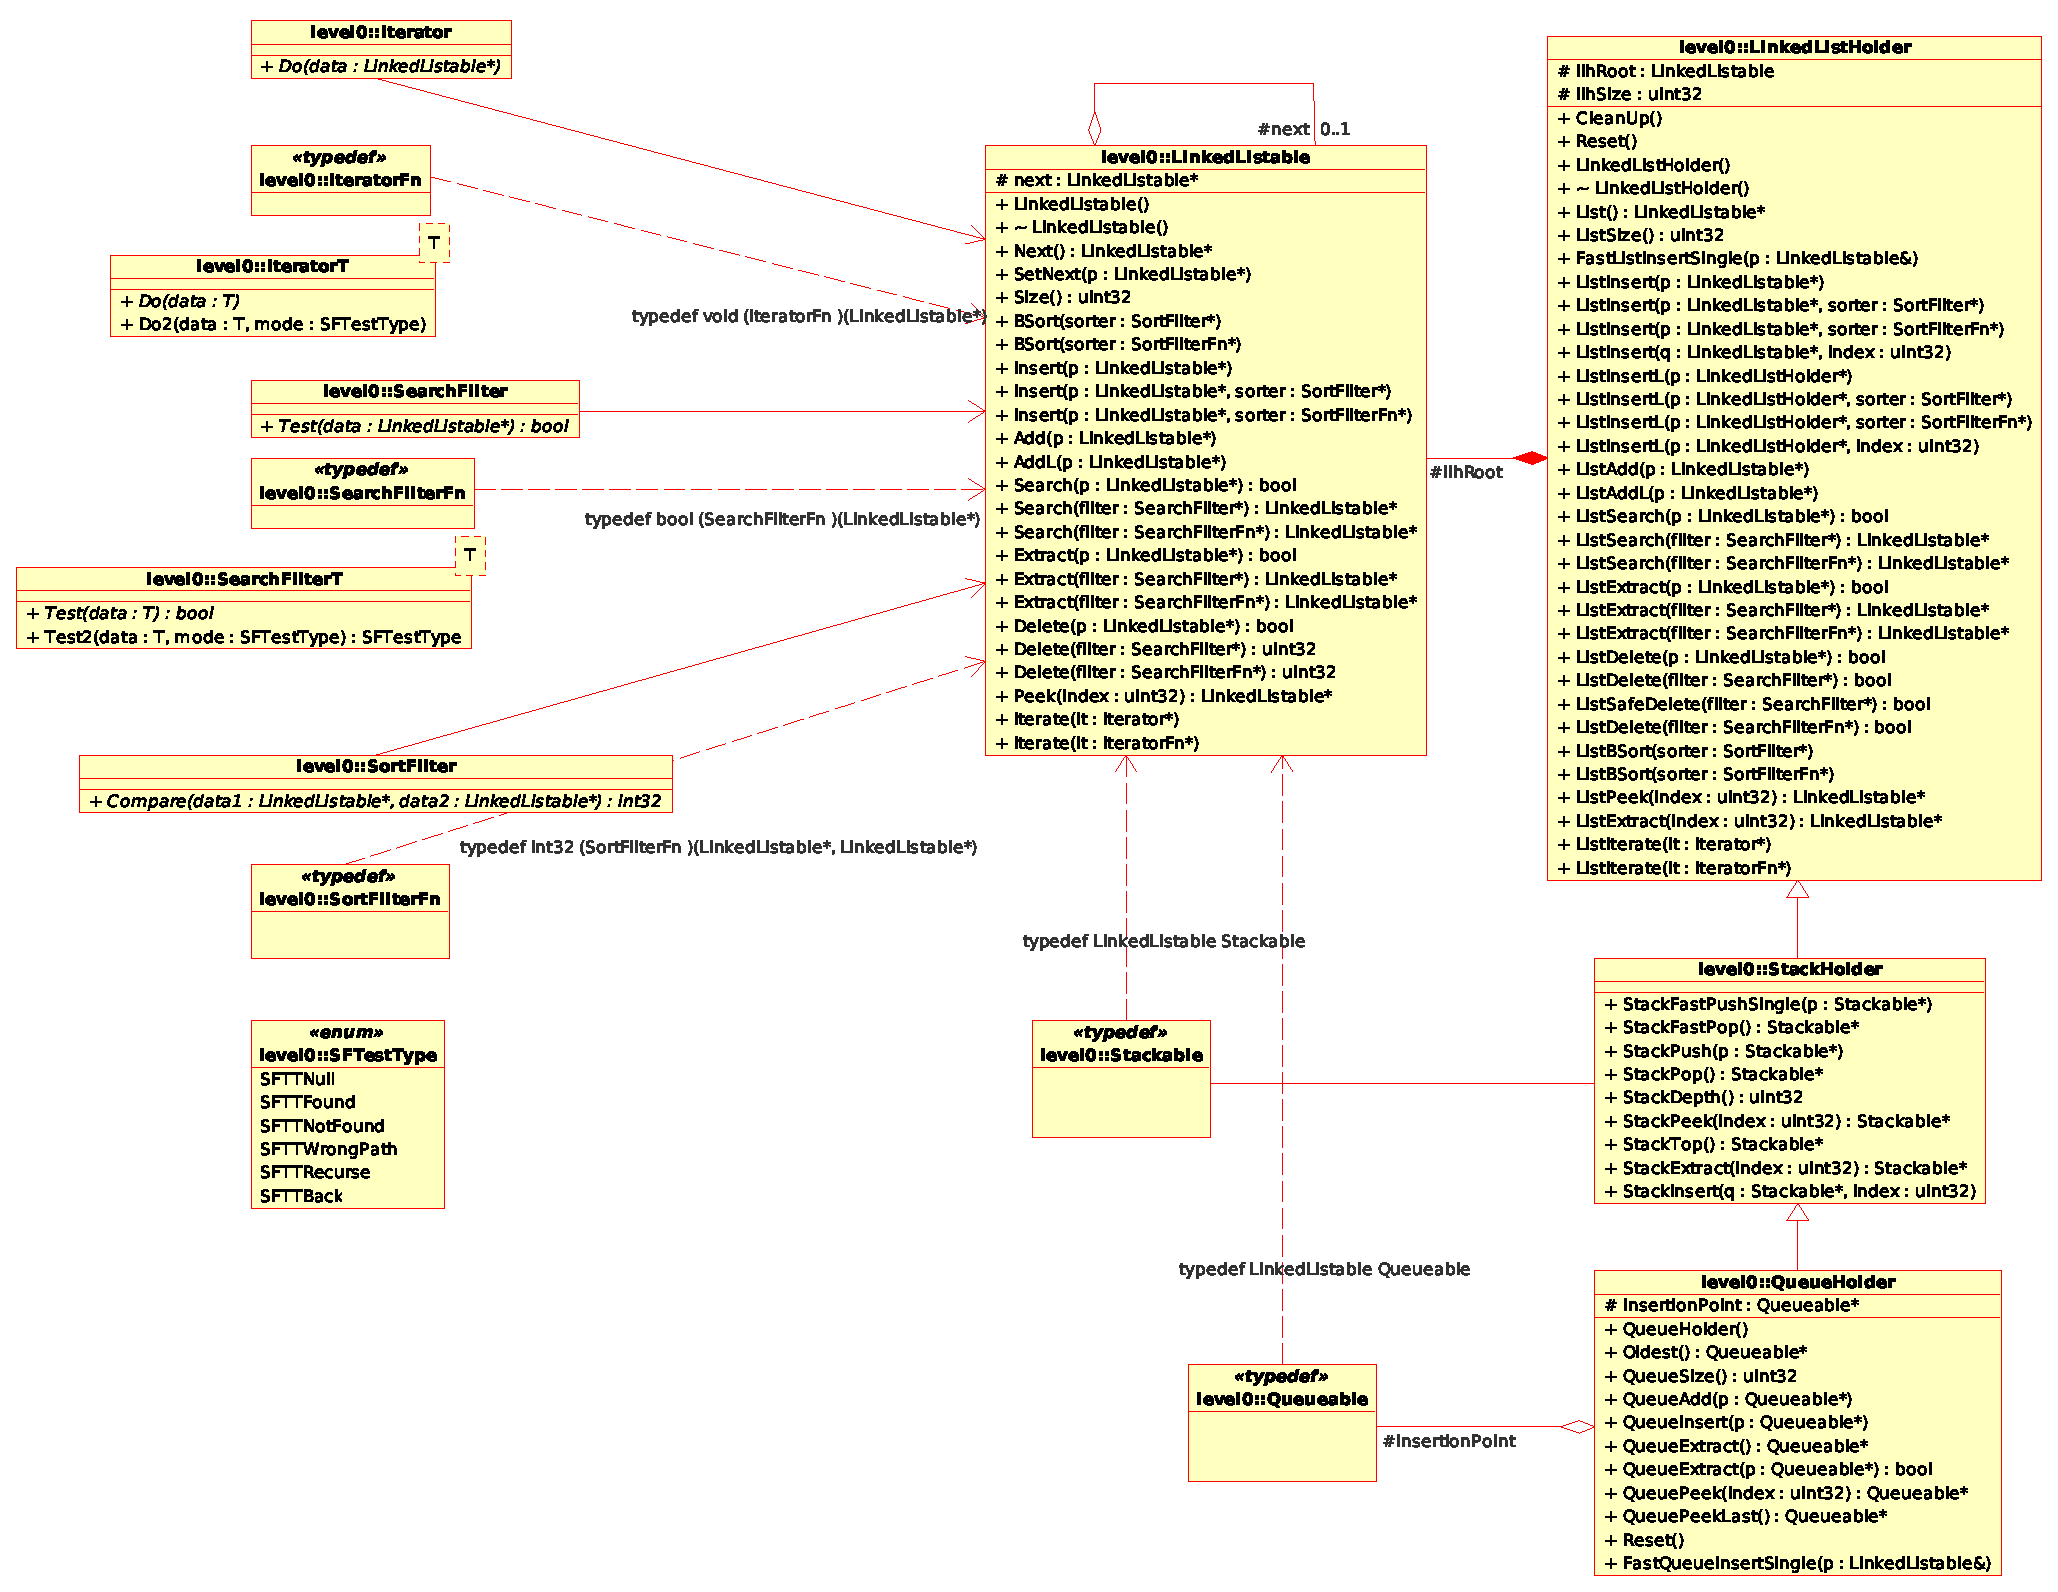
\includegraphics[width=\textwidth]{level0/level0-linked.eps}
  \caption{BaseLib Level0 Linked Lists classes}
  \label{f:level0:linked}
 \end{center}
\end{figure}

Figure \ref{f:level0:linked} depict classes involved in the linked list abstraction offered in BaseLib, the \texttt{directory} abstraction is not presented again. The basic building block of a linked list is a \texttt{LinkedListable} element that is typedefined to became a \texttt{Stackable} and a \texttt{Queueable} object, but is still the same. The modules that you are going to explore are:

\begin{itemize}
 \item LinkedListable

 \item LinkedListHolder
 \item StackHolder
 \item QueueHolder

 \item Iterator, IteratorT, IteratorFn
 \item SearchFilter, SearchFilterT, SearchFilterFn
 \item SortFilter, SortFilterFn
\end{itemize}

Still in this section we discuss about the \texttt{Directory} example that let you puts the hands on the BaseLib \textit{LinkedList} interface.

\begin{itemize}
 \item DirectoryEntry
 \item Directory
\end{itemize}



\subsubsection{LinkedListable}
\texttt{[LinkedListable.h]}\\
 A linked list member. Can be used as root of a linked list, a specific linked list member can be derived from this class (so can be subclassed). The \texttt{LinkedListable} interface must be subclassed to became specific.

A \texttt{LinkedListable} object holds only a pointer to the next \texttt{LinkedListable} object.

\begin{lstlisting}[
extendedchars=true,%
basicstyle=\fontfamily{pcr}\fontseries{m}\selectfont\footnotesize, %
stepnumber=1,%
numberstyle=\tiny,%
keywordstyle=\footnotesize\tt ,%
language=C++]
protected:
   LinkedListable *next;
\end{lstlisting}

The \texttt{Next} method return the pointer to the next \texttt{LinkedListable} object; while using \texttt{SetNext} it is possible to set the attirbute. Such list is a single concatenated linked list, it can be navigated only in one way. The \textit{Size} method count how many \texttt{LinkedListable} iteam are on the list from the object itself, i.e. for example in Figure \ref{f:level0:linkedlist} imagine to be on the second \texttt{tLinkedListable} object from the left, \texttt{Size} will return 4.
The \texttt{BSort} methods will operate like \texttt{Size} on the rightside objects on the list.


\begin{lstlisting}[
extendedchars=true,%
basicstyle=\fontfamily{pcr}\fontseries{m}\selectfont\footnotesize, %
stepnumber=1,%
numberstyle=\tiny,%
keywordstyle=\footnotesize\tt ,%
language=C++]
public:
   LinkedListable *Next()const;
   void SetNext(LinkedListable *p);

   uint32 Size();
   void BSort(SortFilter *sorter);
   void BSort(SortFilterFn *sorter);
\end{lstlisting}


Next functions deal with the insertion and the deletion and the searching activity on a list, probably such functions will be better coded in an iterator, but this is a design choice. \texttt{Insert} method insert the \texttt{LinkedListable} object passed as an argument after the current object in the list. N.B. This method is very powerfull, infact you can also add a list to a list! But be very carefull because if you doesn't want to add a list the \texttt{p*} must be the \texttt{next} attribute resetted to \texttt{NULL}.
\texttt{Add} and \texttt{AddL} add an element or a list to the end of the current queue where the current object, on which you are calling the method, is lying. \texttt{Search} method search downside the list for a matching object. The other two search methods search down the list using a \texttt{SearchFilter} or a \texttt{SearchFilterFn}.

\begin{lstlisting}[
extendedchars=true,%
basicstyle=\fontfamily{pcr}\fontseries{m}\selectfont\footnotesize, %
stepnumber=1,%
numberstyle=\tiny,%
keywordstyle=\footnotesize\tt ,%
language=C++]
   void Insert(LinkedListable *p);
   void Insert(LinkedListable *p,SortFilter *sorter);
   void Insert(LinkedListable *p,SortFilterFn *sorter);

   void Add(LinkedListable *p);
   void AddL(LinkedListable *p);

   bool Search(LinkedListable *p);

   LinkedListable *Search(SearchFilter *filter);
   LinkedListable *Search(SearchFilterFn *filter);
\end{lstlisting}

\texttt{Extract} functions remove the requested element from the list start searching from the next element or using a special filter, returning the requested object if searched and not specified. \texttt{Delete} routines simply search and remove the element requested from the list without returning it, the object will be destroied from the system and no reference will still exists. If the object will be not destroyed the system can suffer of memory leak.

Last few methods are to navigate and browse the linked list.

\begin{lstlisting}[
extendedchars=true,%
basicstyle=\fontfamily{pcr}\fontseries{m}\selectfont\footnotesize, %
stepnumber=1,%
numberstyle=\tiny,%
keywordstyle=\footnotesize\tt ,%
language=C++]
   bool Extract(LinkedListable *p);
   LinkedListable *Extract(SearchFilter *filter);
   LinkedListable *Extract(SearchFilterFn *filter);

   bool Delete(LinkedListable *p);
   uint32 Delete(SearchFilter *filter);
   uint32 Delete(SearchFilterFn *filter);

   LinkedListable *Peek(uint32 index);
   void Iterate(Iterator *it);
   void Iterate(IteratorFn *it);
\end{lstlisting}



\subsubsection{LinkedListHolder}
\texttt{[LinkedListHolder.h]}\\
The \texttt{LinkedListHolder} class is a class that can handle linked lists of \texttt{LinkedListable} objects. As in the schema of Figure \ref{f:level0:linkedlist} a \texttt{LinkedListable} object is structure that hold linked lists and ease the usual operations on such lists (inserting, removing, seraching and sorting).

\begin{figure}[h!]
 \begin{center}
  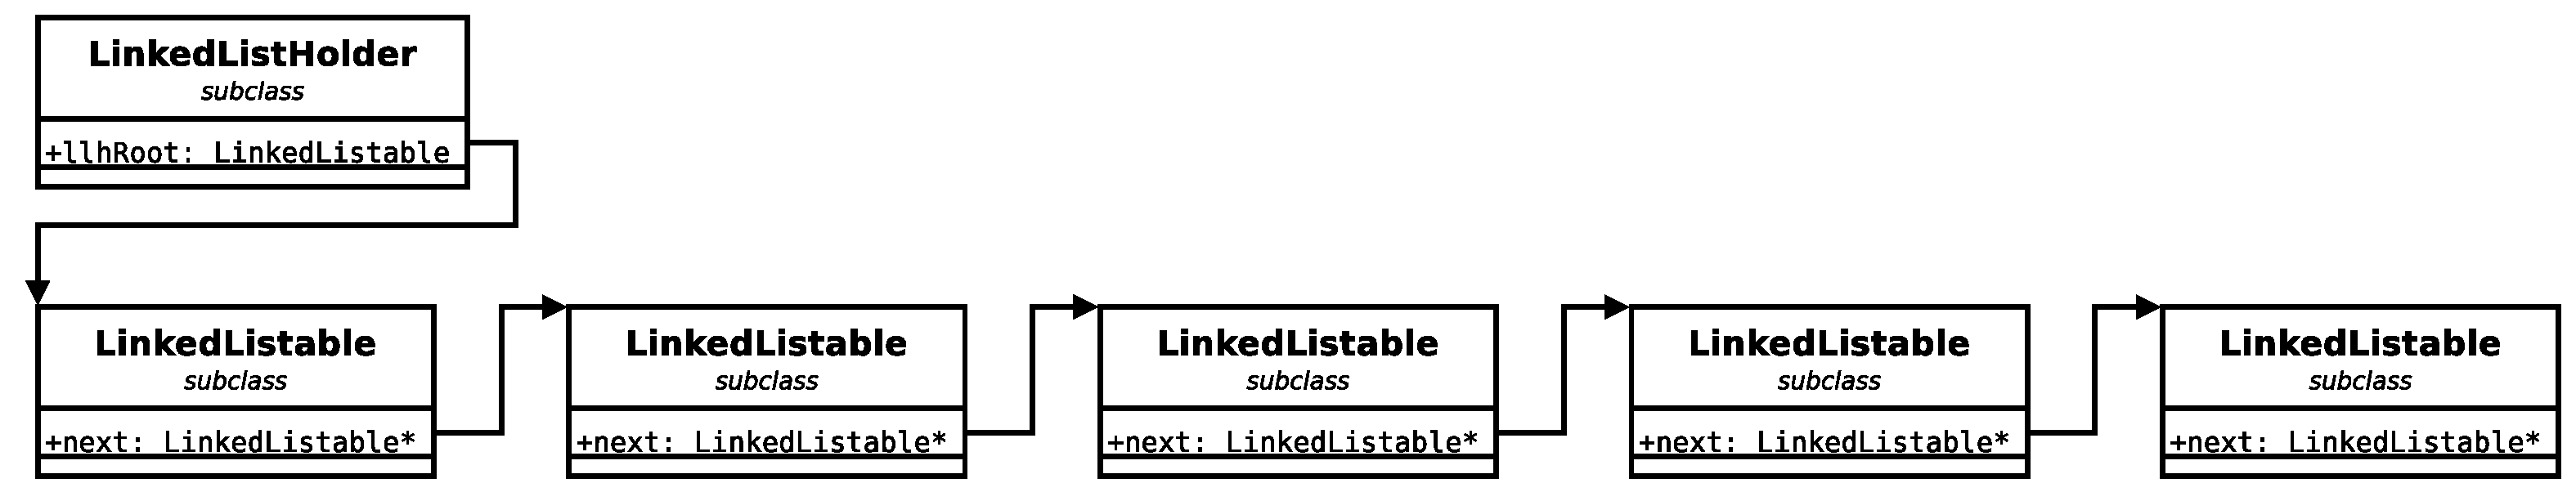
\includegraphics[width=\textwidth]{level0/linkedlist.eps}
  \caption{BaseLib Level0 linked list schema}
  \label{f:level0:linkedlist}
 \end{center}
\end{figure}

A \texttt{LinkedListHolder} is like a list container. Operations on Lists are permitted, the basic informations it holds is the first \texttt{LinkedListable} node of the list and the list size in integers.

\begin{lstlisting}[
extendedchars=true,%
basicstyle=\fontfamily{pcr}\fontseries{m}\selectfont\footnotesize, %
stepnumber=1,%
numberstyle=\tiny,%
keywordstyle=\footnotesize\tt ,%
language=C++]
protected:
   LinkedListable  llhRoot;
   uint32          llhSize;
\end{lstlisting}

\texttt{CleanUp} will deallocate all the contents and then sets the pointer to \texttt{llhRoot->next} to \texttt{NULL} and \texttt{llhSize} to zero, the \texttt{Reset} method does the same but doesn't deallocate content. 

The \texttt{List} method return the first element on the list (\texttt{llhRoot->next}) while \texttt{ListSize} return the size of the linked list (\texttt{llhSize}).

\begin{lstlisting}[
extendedchars=true,%
basicstyle=\fontfamily{pcr}\fontseries{m}\selectfont\footnotesize, %
stepnumber=1,%
numberstyle=\tiny,%
keywordstyle=\footnotesize\tt ,%
language=C++]
public:
   void CleanUp();
   void Reset();

   LinkedListable *List() const;
   uint32 ListSize()const;
\end{lstlisting}

The method \texttt{FastListInsertSingle} insert a single \texttt{LinkedListable} element \texttt{p} as the unique element of the queue.
Overloaded method \texttt{ListInsert} let the user insert a \texttt{LinkedListable} element as the first element or in an ordered way using sorters, rather of \texttt{ListInsertL} manipulate \texttt{LinkedListHolder} elements.\\


Method \texttt{ListAdd} add one single \texttt{LinkedListable} element at the end of the queue; \texttt{ListAddL} add a list of \texttt{LinkedListable} elements at the end of the queue. \\


\begin{lstlisting}[
extendedchars=true,%
basicstyle=\fontfamily{pcr}\fontseries{m}\selectfont\footnotesize, %
stepnumber=1,%
numberstyle=\tiny,%
keywordstyle=\footnotesize\tt ,%
language=C++]
   inline void FastListInsertSingle(LinkedListable &p);
   void ListInsert(LinkedListable *p);
   void ListInsert(LinkedListable *p,SortFilter *sorter);
   void ListInsert(LinkedListable *p,SortFilterFn *sorter);
   void ListInsert(LinkedListable *q,uint32 index);
   void ListInsertL(LinkedListHolder *p);
   void ListInsertL(LinkedListHolder *p,SortFilter *sorter);
   void ListInsertL(LinkedListHolder *p,SortFilterFn *sorter);
   void ListInsertL(LinkedListHolder *p,uint32 index);

   void ListAdd(LinkedListable *p);
   void ListAddL(LinkedListable *p);
\end{lstlisting}

\texttt{ListSearch} methods search the list comparing the element comparing with the one passed by argument or using a \texttt{SearchFilter} or a \texttt{SearchFilterFn}. Overloaded methods \texttt{ListExtract} do the same job as \texttt{ListSearch} but removing the element founded. \texttt{ListDelete} is the same as \texttt{ListExtract} but never return the object founded. Function \texttt{ListSafeDelete} is a special \texttt{ListDelete} version that is safe from reentrance from destructor of object (complex graph destruction). \\


Methods \texttt{ListBSort} simply sort the linked list using the sorter passed as an argument. \texttt{ListPeek} looks into the list an treat it as an array it will return the \texttt{index}-n element of the linked list. \texttt{ListIterate} methods associate an iterator to the linked list. \\


\begin{lstlisting}[
extendedchars=true,%
basicstyle=\fontfamily{pcr}\fontseries{m}\selectfont\footnotesize, %
stepnumber=1,%
numberstyle=\tiny,%
keywordstyle=\footnotesize\tt ,%
language=C++]
   bool ListSearch(LinkedListable *p);
   LinkedListable *ListSearch(SearchFilter *filter);
   LinkedListable *ListSearch(SearchFilterFn *filter);

   bool ListExtract(LinkedListable *p);
   LinkedListable *ListExtract(SearchFilter *filter);
   LinkedListable *ListExtract(SearchFilterFn *filter);
   LinkedListable *ListExtract(uint32 index=0);

   bool ListDelete(LinkedListable *p);
   bool ListDelete(SearchFilter *filter);
   bool ListSafeDelete(SearchFilter *filter);
   bool ListDelete(SearchFilterFn *filter);

   void ListBSort(SortFilter *sorter);
   void ListBSort(SortFilterFn *sorter);

   LinkedListable *ListPeek(uint32 index);

   void ListIterate(Iterator *it);
   void ListIterate(IteratorFn *it);
\end{lstlisting}



\subsubsection{StackHolder}
\texttt{[StackHolder.h]} \\
A stack data structure is simply developed on top of the single linked list abstraction. Inserting (push) elements on the head of the list and removing (pop) elements (one at a time) always from the head of the list. Such operations require only a single linked list (i.e. no double linked list is required). Figure \ref{f:level0:linked} show that a \texttt{StackHolder} is a subclass of a \texttt{LinkedListHolder} so is a linked list container but adds the tipical method a stack will have. \\


The typename \texttt{Stackable} is just a rename of the \texttt{LinkedListable} type, it is defined like below in file \texttt{level0/Iterators.h}.

\begin{lstlisting}[
extendedchars=true,%
basicstyle=\fontfamily{pcr}\fontseries{m}\selectfont\footnotesize, %
stepnumber=1,%
numberstyle=\tiny,%
keywordstyle=\footnotesize\tt ,%
language=C++]
typedef LinkedListable Stackable;
\end{lstlisting}

\texttt{StackFastPushSingle} method and pop's \texttt{StackFastPop} let you push and pop a single \texttt{Stackable} (\texttt{LinkedListable}) element from the stack. \texttt{StackPush} and \texttt{StackPop} are more slow to execute but let you add not a single element but also a linked list (or another stack).

\begin{lstlisting}[
extendedchars=true,%
basicstyle=\fontfamily{pcr}\fontseries{m}\selectfont\footnotesize, %
stepnumber=1,%
numberstyle=\tiny,%
keywordstyle=\footnotesize\tt ,%
language=C++]
public:
   inline void StackFastPushSingle(Stackable *p);
   inline Stackable *StackFastPop();

   void StackPush(Stackable *p);
   Stackable *StackPop();
\end{lstlisting}

Last methods are the same as the \texttt{LinkedListHolder} implementation let only the user call those methods with a more friendly ``stackable'' name.

\begin{lstlisting}[
extendedchars=true,%
basicstyle=\fontfamily{pcr}\fontseries{m}\selectfont\footnotesize, %
stepnumber=1,%
numberstyle=\tiny,%
keywordstyle=\footnotesize\tt ,%
language=C++]
   uint32 StackDepth();
   Stackable *StackPeek(uint32 index);
   Stackable *StackTop();
   Stackable *StackExtract(uint32 index);
   void StackInsert(Stackable *q,uint32 index);
\end{lstlisting}

This class is really simply and each method usually call the same method of the superclass.



\subsubsection{QueueHolder}
\texttt{[QueueHolder.h]}\\
\texttt{QueueHolder} is a class that can handle a queue of \texttt{Queueable} elements; the typename \texttt{Queueable} is just an alias of the \texttt{LinkedListable} type, it is defined like below in file \texttt{level0/Iterators.h}.

\begin{lstlisting}[
extendedchars=true,%
basicstyle=\fontfamily{pcr}\fontseries{m}\selectfont\footnotesize, %
stepnumber=1,%
numberstyle=\tiny,%
keywordstyle=\footnotesize\tt ,%
language=C++]
typedef LinkedListable Queueable;
\end{lstlisting}

A queue data structure is simply depicted in Figure \ref{f:level0:queue}.

\begin{figure}[h!]
 \begin{center}
  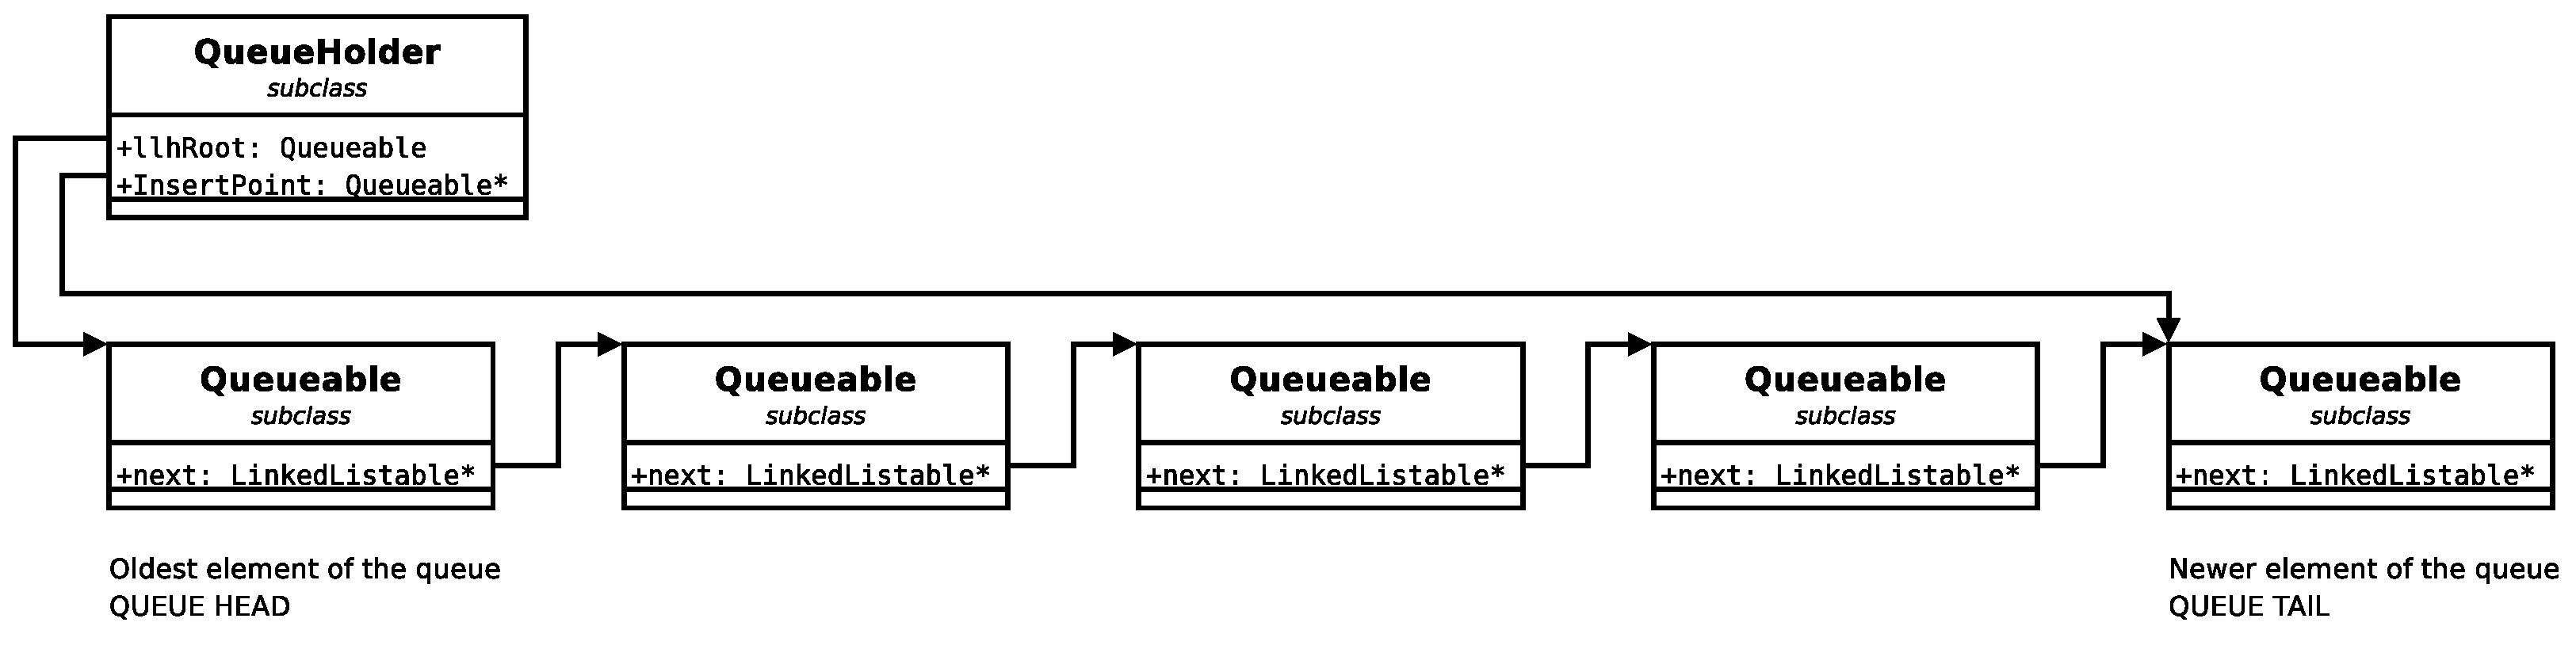
\includegraphics[width=\textwidth]{level0/queue.eps}
  \caption{BaseLib Level0 queue schema}
  \label{f:level0:queue}
 \end{center}
\end{figure}

The \texttt{QueueHolder} class add the protected attribute \texttt{insertionPoint} to the \texttt{StackHolder} class; in this way mantaining only a single linked list with only the \textit{next} pointer it has a full control of the queue knowing the head and tail elements, navigation of the queue remain possible only in one direction, no bidirectional navigation could be possible. In this way removing elements at the tail is very time consuming; the design allows removing elements only from the head of the queue.

\begin{lstlisting}[
extendedchars=true,%
basicstyle=\fontfamily{pcr}\fontseries{m}\selectfont\footnotesize, %
stepnumber=1,%
numberstyle=\tiny,%
keywordstyle=\footnotesize\tt ,%
language=C++]
protected:
   Queueable *insertionPoint;
\end{lstlisting}

The \textit{oldest} element is the element at the head of the queue and is also the oldest added to it. The insertion of a new element will be made at the tail of the queue.\\


The method \texttt{Oldest} return the oldest inserted element in the queue, returning doesn't mean extracting infact the element still reamin in the queue. Note that it is possible to return only one element at a time. The extraction activity is done by the \texttt{QueueExtract} method that return and remove the oldest element on the queue. Last \texttt{QueueExtract} search from the oldest \texttt{Queueable} item the element passed by argument and remove it.\\


The \texttt{QueueAdd} method add on the queue head the passed by \texttt{Queueable} elements, it is possible to add also a list of \texttt{Queueable}s. \texttt{FastQueueInsertSingle} does the same but add to the queue only one element at a time.
\texttt{QueueInsert} insert the passed by argument \texttt{Queueable} element/s resetting all the content of the queue to it/them; use it with care because can remove all elements in the queue.

\begin{lstlisting}[
extendedchars=true,%
basicstyle=\fontfamily{pcr}\fontseries{m}\selectfont\footnotesize, %
stepnumber=1,%
numberstyle=\tiny,%
keywordstyle=\footnotesize\tt ,%
language=C++]
public:
   Queueable *Oldest();
   Queueable *QueueExtract();
   bool QueueExtract(Queueable *p);

   void QueueAdd(Queueable *p); 
   inline void FastQueueInsertSingle(LinkedListable &p);
   void QueueInsert(Queueable *p);
\end{lstlisting}

Methods \texttt{QueuePeek} and \texttt{QueuePeekLast} do not remove the required element from the queue; the first one do not do any check on queue boundary before performing the peek action.
\texttt{Reset} method simply call the superclass one removing one by one elements from the list. Elements could be not more refereneced and so can be lost wasting memory.

\begin{lstlisting}[
extendedchars=true,%
basicstyle=\fontfamily{pcr}\fontseries{m}\selectfont\footnotesize, %
stepnumber=1,%
numberstyle=\tiny,%
keywordstyle=\footnotesize\tt ,%
language=C++]
   Queueable *QueuePeek(uint32 index);
   Queueable *QueuePeekLast();

   void Reset();
   uint32 QueueSize();
\end{lstlisting}



\subsubsection{Iterator, IteratorT, IteratorFn}
\texttt{[Iterator.h]}\\
The \texttt{Iterator} class define only one pure virtual function so it is a C++ interface. The function is defined as:

\begin{lstlisting}[
extendedchars=true,%
basicstyle=\fontfamily{pcr}\fontseries{m}\selectfont\footnotesize, %
stepnumber=1,%
numberstyle=\tiny,%
keywordstyle=\footnotesize\tt ,%
language=C++]
public:
   virtual void Do (LinkedListable* data)=0;
\end{lstlisting}

The \texttt{Do} function perform the iteration passing a \texttt{LinkedListable} element as an argument. 
\texttt{IteratorT} is a more specialised version of the \texttt{Iterator} letting the developer not to specify a \texttt{LinkedListable} element or a subclass of it in the \texttt{Do} method. \texttt{IteratorT} is also an interface.

\texttt{IteratorFn} is simply a typedef defined as follow:

\begin{lstlisting}[
extendedchars=true,%
basicstyle=\fontfamily{pcr}\fontseries{m}\selectfont\footnotesize, %
stepnumber=1,%
numberstyle=\tiny,%
keywordstyle=\footnotesize\tt ,%
language=C++]
typedef void (IteratorFn )(LinkedListable* data);
\end{lstlisting}



\subsubsection{SearchFilter, SearchFilterT, SearchFilterFn}
\texttt{[Iterator.h]}\\
The \texttt{SearchFilter} class define only one pure virtual function so it is a C++ interface. The function is defined as:

\begin{lstlisting}[
extendedchars=true,%
basicstyle=\fontfamily{pcr}\fontseries{m}\selectfont\footnotesize, %
stepnumber=1,%
numberstyle=\tiny,%
keywordstyle=\footnotesize\tt ,%
language=C++]
public:
   virtual bool Test (LinkedListable* data)=0;
\end{lstlisting}

The \texttt{Test} function perform the search on a set of data passing a \texttt{LinkedListable} element as an argument. A new class that implement the searching activity must be defined.
\texttt{SearchFilterT} is a more specialised version of the \texttt{SearchFilter} letting the developer not to specify a \texttt{LinkedListable} element or a subclass of it in the \texttt{Test} method. \texttt{SearchFilterT} is also an interface.

\texttt{SearchFilterFn} is simply a typedef defined as follow:

\begin{lstlisting}[
extendedchars=true,%
basicstyle=\fontfamily{pcr}\fontseries{m}\selectfont\footnotesize, %
stepnumber=1,%
numberstyle=\tiny,%
keywordstyle=\footnotesize\tt ,%
language=C++]
typedef bool (SearchFilterFn )(LinkedListable* data);
\end{lstlisting}



\subsubsection{SortFilter, SortFilterFn}
\texttt{[Iterator.h]}\\
The \texttt{Iterator} class define only one pure virtual function so it is a C++ interface. The function is defined as:

\begin{lstlisting}[
extendedchars=true,%
basicstyle=\fontfamily{pcr}\fontseries{m}\selectfont\footnotesize, %
stepnumber=1,%
numberstyle=\tiny,%
keywordstyle=\footnotesize\tt ,%
language=C++]
public:
   virtual void Do (LinkedListable* data)=0;
\end{lstlisting}

The \texttt{Do} function perform the iteration passing a \texttt{LinkedListable} element as an argument. 
\texttt{IteratorT} is a more specialised version of the \texttt{Iterator} letting the developer not to specify a \texttt{LinkedListable} element or a subclass of it in the \texttt{Do} method. \texttt{IteratorT} is also an interface.

\texttt{IteratorFn} is simply a typedef defined as follow:

\begin{lstlisting}[
extendedchars=true,%
basicstyle=\fontfamily{pcr}\fontseries{m}\selectfont\footnotesize, %
stepnumber=1,%
numberstyle=\tiny,%
keywordstyle=\footnotesize\tt ,%
language=C++]
typedef void (IteratorFn )(LinkedListable* data);
\end{lstlisting}

TODO \\
TODO \\
TODO \\
thanks Ric \\
aggiugere qualche esempio di utilizzo (ps prendi il libro di dati e algoritmi)


\subsubsection{DirectoryEntry}
\texttt{[Directory.h]}
Such \texttt{DirectoryEntry} class represent a file or a subdirectory. Usually a directory structure is a tree data structure but such class is implemented using a single linked list; this abstraction doesn't represent a tree of files or directories but simply the directory content, letting navigate in an OS directory.\\


There are three private attributes: the file or subdirectory name, some statistics about the file and a pointer to a \texttt{Directory} conteiner that is a \texttt{LinkedListHolder}.

\begin{lstlisting}[
extendedchars=true,%
basicstyle=\fontfamily{pcr}\fontseries{m}\selectfont\footnotesize, %
stepnumber=1,%
numberstyle=\tiny,%
keywordstyle=\footnotesize\tt ,%
language=C++]
private:
   const char* fname;
   struct stat fileStatistics;
   Directory* holder;
\end{lstlisting}

Such attributes let the \texttt{Directory} and \texttt{DirectoryEntry} classes change the \texttt{LinkedListHolder} and \texttt{LinkedListable} structure to showed in Figure \ref{f:level0:directory}.

\begin{figure}[h!]
 \begin{center}
  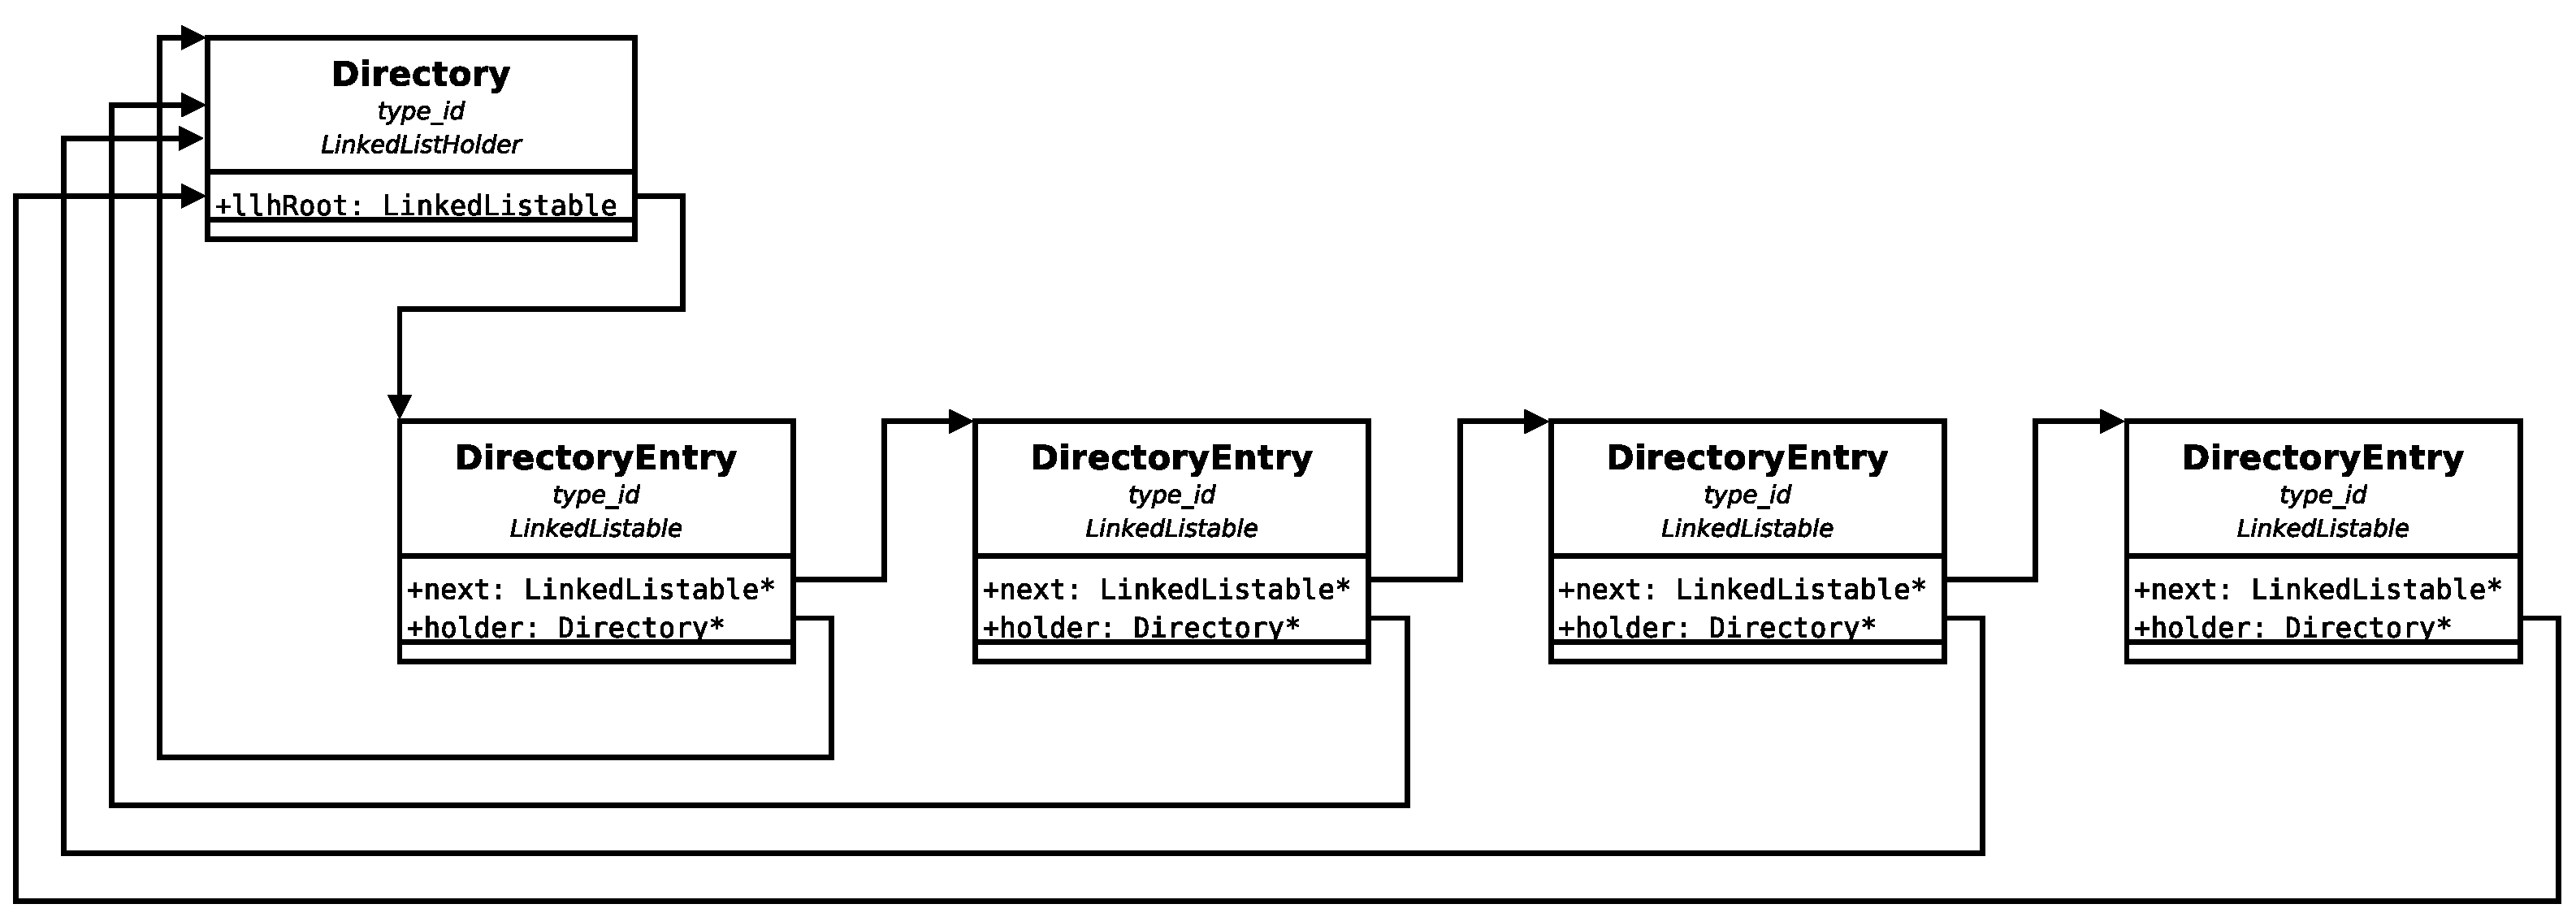
\includegraphics[width=\textwidth]{level0/directory.eps}
  \caption{BaseLib Level0 Directory scheme}
  \label{f:level0:directory}
 \end{center}
\end{figure}

A creation time the developer must supply the \texttt{Directory} container and the name of the file or subdirectory.
The \texttt{Name} method return the name of the file or subdirectory and the methods \texttt{IsDirectory} and \texttt{IsFile} let you check if the instance represent a directory or a file.


\texttt{ReadOnly} let you query if the file has the \textit{read only} attribute, \texttt{Size} method return the size of the file. The method \texttt{Time} return the last write time and \texttt{LastAccessTime} get the last access time.

\begin{lstlisting}[
extendedchars=true,%
basicstyle=\fontfamily{pcr}\fontseries{m}\selectfont\footnotesize, %
stepnumber=1,%
numberstyle=\tiny,%
keywordstyle=\footnotesize\tt ,%
language=C++]
public:
   DirectoryEntry(Directory *holder, const char *fname = NULL);
   ~DirectoryEntry();

   const char* Name();
   bool IsDirectory();
   bool IsFile();

   bool ReadOnly();
   int64 Size();

   time_t Time();
   time_t LastAccessTime();
\end{lstlisting}



\subsubsection{Directory}
\texttt{[Directory.h]}
The \texttt{Directory} class contains information about a directory and all its content. It basically hold a single linked list of \texttt{DirectoryEntry} that can be file and/or subdirectory names. \\


A \texttt{Directory} is identified by a path in the FileSystem hierical on each common OS nowadays. So the first attribute of the class is the path of the directory to be listed \texttt{baseAddress}; the second attribute is the size of the entire directory \texttt{size}.

\begin{lstlisting}[
extendedchars=true,%
basicstyle=\fontfamily{pcr}\fontseries{m}\selectfont\footnotesize, %
stepnumber=1,%
numberstyle=\tiny,%
keywordstyle=\footnotesize\tt ,%
language=C++]
private:
   char* baseAddress;
   uint64 size;
\end{lstlisting}

Such class has only few methods; the constructor does the major stuff. The constructor require the path of the directory a file mask and a sorter, in this way it is possible to have a list of only the file of a certain format.
\texttt{TotalFileSize} simply return the \texttt{size} attribute.\\


The two static methods are currently coded only for Windows platforms and let the user create a directory and test for directory existance.

\begin{lstlisting}[
extendedchars=true,%
basicstyle=\fontfamily{pcr}\fontseries{m}\selectfont\footnotesize, %
stepnumber=1,%
numberstyle=\tiny,%
keywordstyle=\footnotesize\tt ,%
language=C++]
public:
   Directory(const char* address,const char* fileMask="*",SortFilterFn* sorter=NULL);
   uint64 TotalFileSize();

   static bool Create(const char* address);
   static bool DirectoryExists(const char* address);
\end{lstlisting}



\subsection{Static Lists}
\begin{figure}[h!]
 \begin{center}
  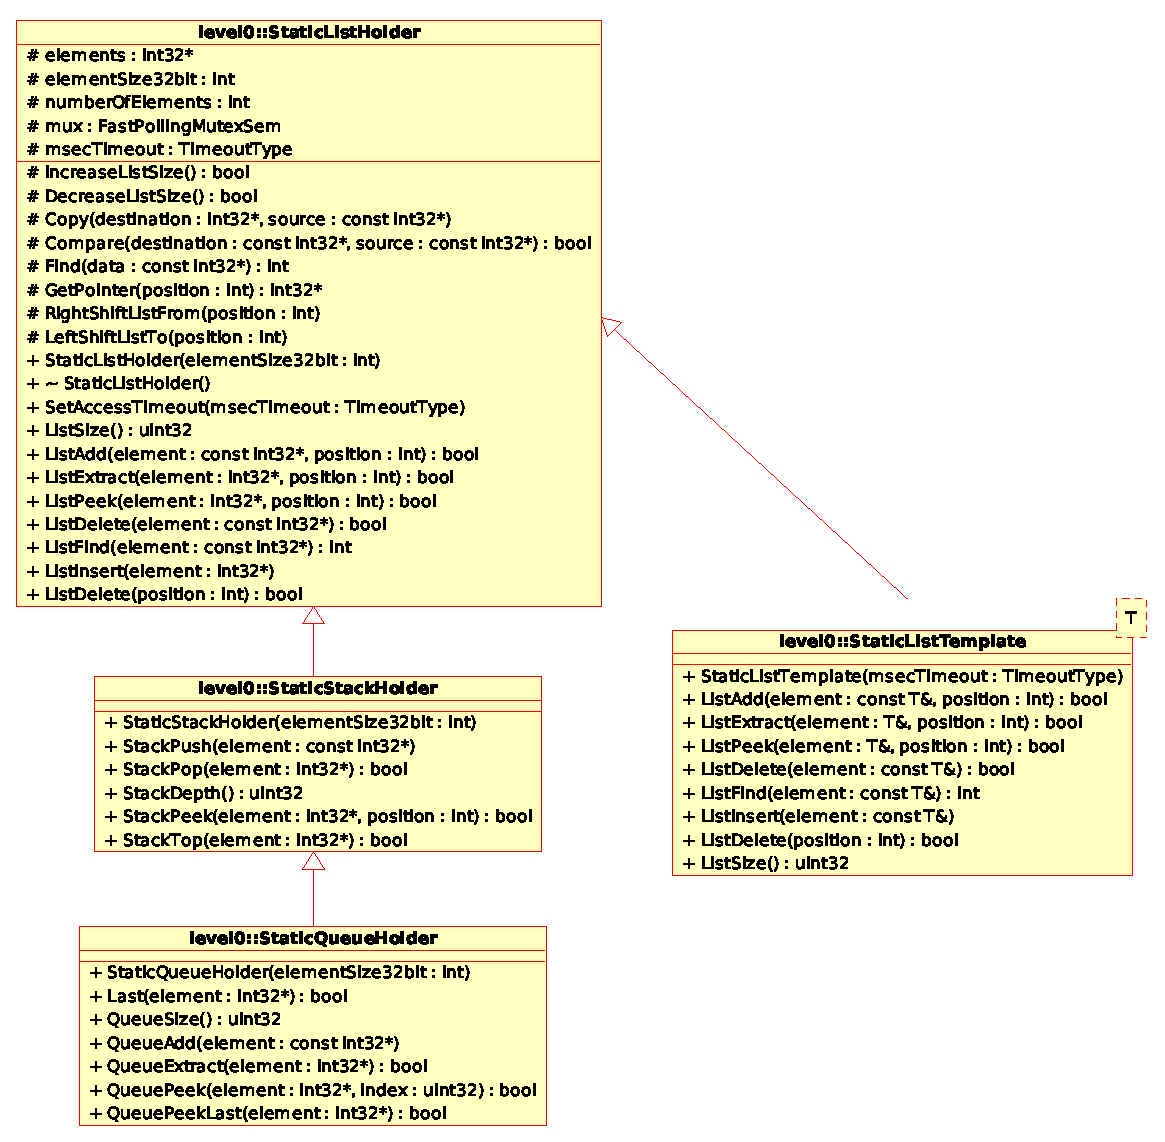
\includegraphics[width=0.55\textwidth]{level0/level0-static.eps}
  \caption{BaseLib Level0 Static Lists classes}
  \label{f:level0:static}
 \end{center}
\end{figure}

Static Lists are basically \textit{arrays} or \textit{vectors}. Such structure contains 32bit pointers or any other structure. This list of pointers can grow and shrink and the reallocation is done by the class itself using library routines like \texttt{malloc} and \texttt{realloc}. It obvioulsy allows inserting and removing of elements. It also offers the possibility to control the data access via a semaphore.


Class diagram is depicted in Figure \ref{f:level0:static}, classe in this group are:

\begin{itemize}
 \item StaticListHolder
 \item StaticStackHolder
 \item StaticQueueHolder

 \item StaticListTemplate
\end{itemize}

Static list classes are written with the aim of mantaining the same methods signatures of the Linked List interface.



\subsubsection{StaticListHolder}
\texttt{[StaticListHolder.h]}\\
The main data structure that hold all the data is an array; this array is dynamically allocated at run-time and is pointed from the \texttt{elements} attribute. Such pointer point to 32bit integers, this integers are usually 32bit pointers, but can be also a structures of the same size; the constructor let you create an array with elements of a size multiple of 32bit. So the \textit{StaticList} can hold 32bit ptr or 64bit ptr or any other structure.
The protected attribute \texttt{elementSize32bit} give you the size of one item on the \textit{StaticList}; the \texttt{numberOfElements} give the number of items in the \textit{StaticList}, the \texttt{FastPollingMutexSem} give a way to allow multiple threads protected access to the data and the \texttt{msecTimeout} is the timeout to wait on the semaphore for catching the resource.

\begin{lstlisting}[
extendedchars=true,%
basicstyle=\fontfamily{pcr}\fontseries{m}\selectfont\footnotesize, %
stepnumber=1,%
numberstyle=\tiny,%
keywordstyle=\footnotesize\tt ,%
language=C++]
protected:
   int32* elements;
   int elementSize32bit;
   int numberOfElements;

   FastPollingMutexSem mux;
   TimeoutType msecTimeout;
\end{lstlisting} 

The following protected methods are self explained and are used to grow and shrink the ata structure, copy and move datas and finding and indexing an element in the \texttt{StaticListHolder}. Comments are left.

\begin{lstlisting}[
extendedchars=true,%
basicstyle=\fontfamily{pcr}\fontseries{m}\selectfont\footnotesize, %
stepnumber=1,%
numberstyle=\tiny,%
keywordstyle=\footnotesize\tt ,%
language=C++]
   /** increases the list size by 1.
       Manages the reallocation of memory when necessary */
   bool IncreaseListSize();
   /** decreases the list size by 1.
       Reallocation of memory is not performed */
   bool DecreaseListSize();

   /** copies data from a buffer to the position */
   inline void Copy(int32 *destination,const int32 *source);
   /** compares data between source and destination. True means equal */
   inline bool Compare(const int32 *destination,const int32 *source);
   /** finds data in list. -1 means not found */
   inline int Find(const int32 *data);

   /** retrieves address of data element */
   inline int32* GetPointer(int position);
   /** moves all the pointers from position to the right.
       Assumes that the last position is empty */
   inline void RightShiftListFrom(int position);
   /** removes the element in position and shifts all the elements 
       at the right of it to the left */
   inline void LeftShiftListTo(int position);
\end{lstlisting}

Public methods have the same names as \texttt{LinkedListHolder}'s methods, arguments differ. The size of the elements, in 4byte units, is defined by the constructor and is no more modificable.\\


To control multiple access it is possible to set a timeout on the waiting operation, the timeout can be set with \texttt{SetAccessTimeout}. To retrieve the number of elements in the \texttt{StaticList} use \texttt{ListSize}.\\


\texttt{ListAdd} add one element at any specified position; as a shortcut if the element must be added at the top of the list you can pass 0 as at position argument and -1 for the end of the list; \texttt{ListInsert} simply add the element at the top of the array.

The method \texttt{ListFind} finds at what index the specified data is located, it returns -1 if doesn't found any matching object.

\texttt{ListExtract} removes an element from any position, if \texttt{position} is 0 it removes from the top, if -1 removes from the end; \texttt{element} is a pointer to a buffer of data that the will be filled by the method. \texttt{ListPeek} reads an item from the data structure without affecting the list; \texttt{element} argument is a pointer to a buffer of data that will be copied from the list. The method \texttt{ListDelete} removes an element from the list using a copy of the \texttt{element} as a search key. The last \texttt{ListDelete} removes at the specified indexed position.

\begin{lstlisting}[
extendedchars=true,%
basicstyle=\fontfamily{pcr}\fontseries{m}\selectfont\footnotesize, %
stepnumber=1,%
numberstyle=\tiny,%
keywordstyle=\footnotesize\tt ,%
language=C++]
public:
   StaticListHolder(int elementSize32bit = 1);
   virtual ~StaticListHolder();

   void SetAccessTimeout(TimeoutType  msecTimeout = TTInfiniteWait);
   uint32 ListSize()const;

   bool ListAdd(const int32 *element,int position = SLH_EndOfList);
   inline void ListInsert(int32 *element);

   int ListFind(const int32 *element);

   bool ListExtract(int32 *element=NULL,int position = SLH_EndOfList);
   bool ListPeek(int32 *element=NULL,int position = SLH_EndOfList);
   bool ListDelete(const int32 *element);
   inline bool ListDelete(int position);
\end{lstlisting}



\subsubsection{StaticStackHolder}
\texttt{[StaticStackHolder.h]}\\
This class is try to mimic the same API of StackHolder but relaying on arrays.
The constructor creates a stack with the given element size (note that the size is in 32 bit multiples), the size of the stack my vary during run time.
\texttt{StackPush} insert on top a single element. When the space is finished the bottom is discarded; \texttt{StackPop} get an element from top of the array and remove it from the stack; for not removing the element from the stack use \texttt{StackTop}.
Method \texttt{StackPeek} looks into the stack for an element with the given index \texttt{position}.
\texttt{StackDepth} return the number of elements in the stack.

\begin{lstlisting}[
extendedchars=true,%
basicstyle=\fontfamily{pcr}\fontseries{m}\selectfont\footnotesize, %
stepnumber=1,%
numberstyle=\tiny,%
keywordstyle=\footnotesize\tt ,%
language=C++]
public:
   StaticStackHolder(int elementSize32bit=1);

   inline void StackPush(const int32* element);
   inline bool StackPop(int32* element);
   inline bool StackTop(int32* element);
   inline bool StackPeek(int32* element,int position);

   inline uint32 StackDepth();
\end{lstlisting}



\subsubsection{StaticQueueHolder}
\texttt{[StaticQueueHolder.h]}\\
This class is still try to mimic the same API of QueueHolder but relaying on arrays.
Like the \texttt{StaticStackHolder} and the superclass \texttt{StatiListHolder} this class require the size of the elements in 32bit units in the constructor. \texttt{QueueSize} return the number of elements in the queue.
\texttt{QueueAdd} insert an element on the queue, \texttt{Last} return the last inserted element in the queue, \texttt{QueueExtract} removes the oldest element from the queue; \texttt{QueuePeek} looks into the queue, index 0 is the most recent added; \texttt{QueuePeekLast} looks into the queue to the last element inserted.

\begin{lstlisting}[
extendedchars=true,%
basicstyle=\fontfamily{pcr}\fontseries{m}\selectfont\footnotesize, %
stepnumber=1,%
numberstyle=\tiny,%
keywordstyle=\footnotesize\tt ,%
language=C++]
public:
   StaticQueueHolder(int elementSize32bit = 1);

   inline void QueueAdd(const int32* element);
   inline bool Last(int32* element);
   inline bool QueueExtract(int32* element);
   inline bool QueuePeek(int32* element,uint32 index);
   inline bool QueuePeekLast(int32* element);

   inline uint32 QueueSize();
\end{lstlisting}



\subsubsection{StaticListTemplate}
\texttt{[StaticListTemplate.h]}\\
This class is a template to customise a \texttt{StaticListHolder} for a specific struct or class. Such class is a subclass of the \texttt{StaticListHolder}. This class is never used in BaseLib. This class lets specializing the superclass for a particular type of object. Using such specialized class you have an array of object of the same size of the object templatized for. The interface, really similar to the \texttt{StaticListHolder} one follows.

\begin{lstlisting}[
extendedchars=true,%
basicstyle=\fontfamily{pcr}\fontseries{m}\selectfont\footnotesize, %
stepnumber=1,%
numberstyle=\tiny,%
keywordstyle=\footnotesize\tt ,%
language=C++]
public:
   StaticListTemplate(TimeoutType  msecTimeout = TTInfiniteWait);

   inline bool ListAdd(const T &element,int position=SLH_EndOfList)
   inline void ListInsert(const T &element);

   inline bool ListExtract(T &element,int position=SLH_EndOfList)
   inline bool ListPeek(T &element,int position = SLH_EndOfList)
   inline bool ListDelete(const T &element);
   inline bool ListDelete(int position);

   inline int ListFind(const T &element);

   uint32 ListSize()const;
\end{lstlisting}



\subsection{Design Notes}

There is no need to typedef \texttt{LinkedListable} in \texttt{Stackable} and \texttt{Queueable} but is not an error, if there is no need to extend it with further information why aliasing it? A good choice could be to extend \texttt{LinkedListable} in \texttt{Queueable} creating a double linked list that could be a real advantage to boost the performance of walking a list.\\

 (why not call them symmetrically? Like \texttt{StackFastPush} and \texttt{StackFastPop}) \\
(those function can have a more significant name like \texttt{QueueOldest} and \texttt{QueueExtract}) \\
The \texttt{QueueAdd} method add on the queue head the passed by \texttt{Queueable} elements, it is possible to add also a list of \texttt{Queueable}s. \texttt{FastQueueInsertSingle} does the same but add to the queue only one element at a time. This is another misusage of names in this section: better names can be \texttt{QueueAdd} and \texttt{QueueAddFast}. \\


Some methods, like \texttt{queueInsert} are to be used with care. \texttt{queueInsert} add elements to the queue deleting all other elements in the queue without any check or call to deletion wasting all references.\\


Sometimes there are no boundaries checks in the \textit{linked} implementation but also in the \textit{static} implementation.\\


Probably there is a lack of a Template, look at \textit{level0/Iterator.h} there are those declariotions: \texttt{Iterator}, \texttt{IteratorFn}, \texttt{IteratorT}; \texttt{SearchFilter}, \texttt{SearchFilterFn}, \texttt{SearchFilterT}; \texttt{SortFilter}, \texttt{SortFiletrFn} and \texttt{SortFilterT} is not defined.\\


The \texttt{Directory} pair of classes must be ported also on other OSes. The \texttt{Driectory} structure can be developed on a tree data structure instead on a single linked list. So there is the need to add the tree data structure to this data structure section. \\


The \texttt{StaticQueue} structure will be better developed on a circular buffer instead on a \texttt{StaticListHolder}. Will be more processor efficient.\\



\section{IPC}
This group of classes add the semaphore abstraction and the spinlock mechanism to the BaseLib library. Figure \ref{f:level0:ipc} illustrate the classes structure, semaphores and spinlocks, of a great interest is the \textit{SemNameDataBase}.

\begin{figure}[h!]
 \begin{center}
  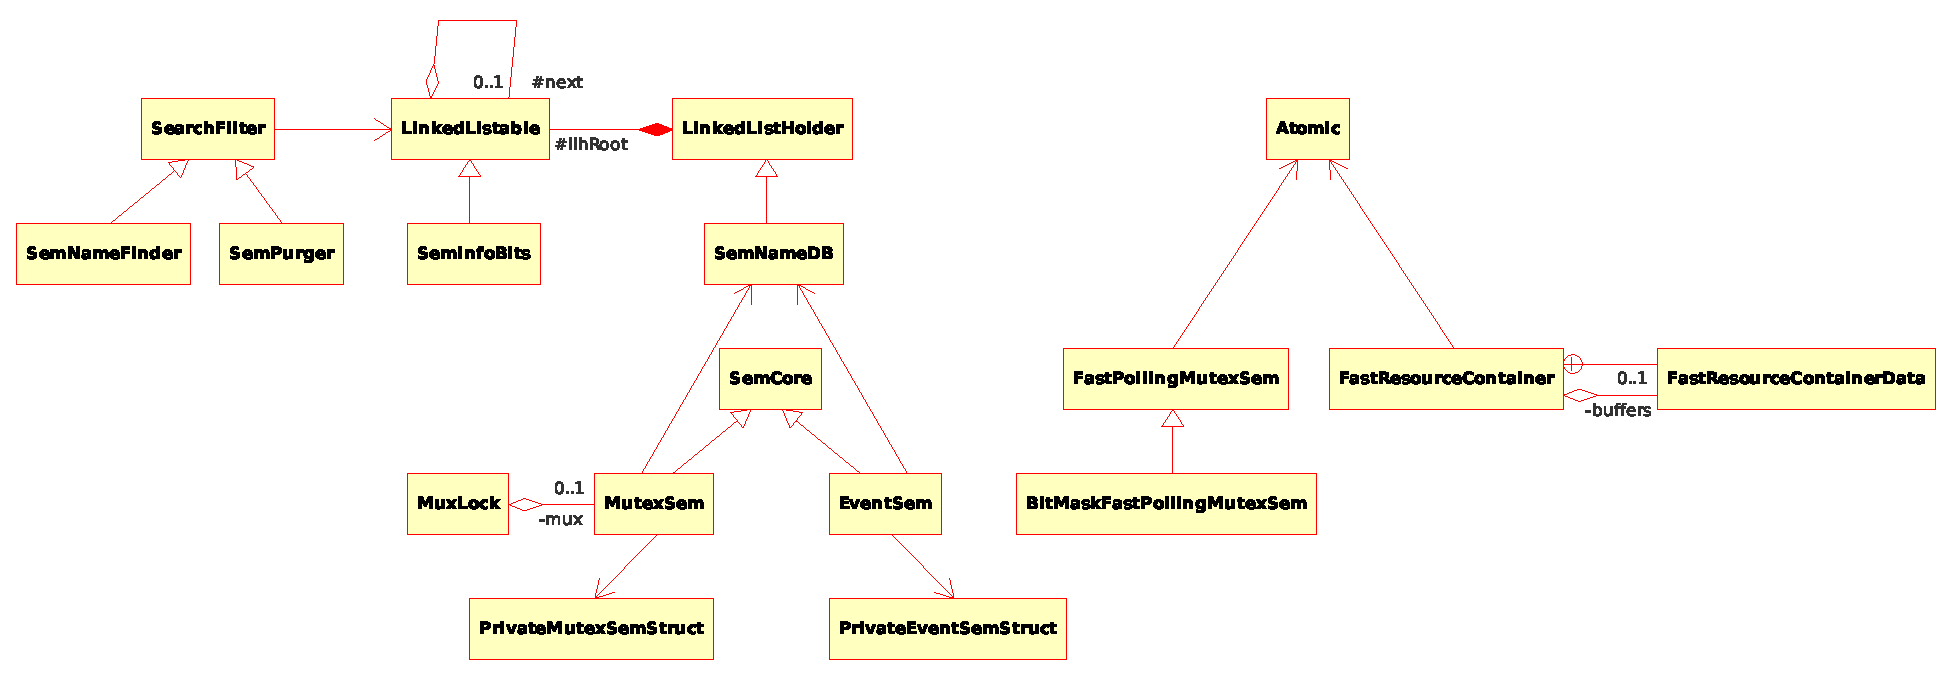
\includegraphics[width=\textwidth]{level0/level0-IPC.eps}
  \caption{BaseLib Level0 IPC classes}
  \label{f:level0:ipc}
 \end{center}
\end{figure}



\subsection{Semaphores}
A semaphore is one of the simplest Inter Processes Communication mechanisms. BaseLib introduce different types of semaphores. One of the most important functionality it adds is the \textit{SemNameDataBase} that is a list of all BaseLib's semaphores created run-time. Such stuff lets the developer exploits named semaphores on each Operating System.

\begin{figure}[h!]
 \begin{center}
  \includegraphics[width=\textwidth]{level0/level0-IPC-Sem.eps}
  \caption{BaseLib Level0 semaphore classes}
  \label{f:level0:ipc-sem}
 \end{center}
\end{figure}

Figure \ref{f:level0:ipc-sem} depict semaphore classes in this section (other classes previously anlized are also present: \texttt{LinkedListable}, \texttt{LinkedListHolder} and \texttt{SearchFilter}):
\begin{itemize}
 \item SemInfoBits
 \item SemNameDB
 \item SemNameFinder, SemPurger

 \item SemCore
 \item EventSem
 \item MutexSem
 \item MuxLock
\end{itemize}

We are going first to explore the \textit{SemNameDataBase} architecture. The OS2 naming convention is used in this group of classes, in OS2 there are \texttt{EventSem} and \texttt{MutexSem}. Follow a table that summarizes some differences between ipc's API in OS/2, POSIX.1b (UNIX, System V) and POSIX.1c (pthread). The mapping between OS/2 and POSIX.1b is not straightforward.

\begin{table}[!h]
 \begin{center}
  \begin{tabular}{|l|l|l|}
   \hline
    OS/2 & POSIX.1c & POSIX.1b \\
   \hline
    \texttt{DosCreateMutexSem} & \texttt{pthread\_mutex\_init} & \texttt{sem\_init} \\
   \hline
    \texttt{DosRequestMutexSem} & \texttt{pthread\_mutex\_lock} / & \texttt{sem\_wait} / \\
     & \texttt{pthread\_mutex\_trylock} & \texttt{sem\_trywait} \\
   \hline
    \texttt{DosReleaseMutexSem} & \texttt{pthread\_mutex\_unlock} & \texttt{sem\_post} \\
   \hline
    \texttt{DosCloseMutexSem} & \texttt{pthread\_mutex\_destroy} & \texttt{sem\_destroy} \\
   \hline
    \texttt{DosCreateEventSem} & \texttt{pthread\_cond\_init} & \texttt{sem\_init} \\
   \hline
    \texttt{DosWaitEventSem} & \texttt{pthread\_cond\_signal\_wait} / & \texttt{sem\_wait} / \\
     & \texttt{pthread\_cond\_timedwait} & \texttt{sem\_trywait} \\
   \hline
    \texttt{DosPostEventSem} & \texttt{pthread\_cond\_signal} / & \texttt{sem\_post} \\
     & \texttt{pthread\_cond\_broadcast} & \\
   \hline
    \texttt{DosCloseEventSem} & \texttt{pthread\_cond\_destroy} & \texttt{sem\_destroy} \\
   \hline
   \end{tabular}
   \end{center}
  \caption{Basic IPC in OS2, POSIX.1b (UNIX, System V) and POSIX.1c (pthread)}
 \label{t:ipc_api}
\end{table}

Table \ref{t:ipc_api} must clarify the mapping between \textit{EventSem} in OS/2 and \textit{Conditional Variables} in POSIX.1c and between \textit{MutexSem} and \textit{mutex} in POSIX.1c.



\subsubsection{SemInfoBits}
\texttt{[SemCore.cpp]}\\
The class \texttt{SemInfoBits} is a \texttt{LinkedListable} list item of the \texttt{SemNameDataBase} (that is a \texttt{LinkedListHolder}). There is a \texttt{SemInfoBits} list item for each semaphore istantiated in the library, for each semaphore in the DataBase we save a \texttt{name}, an \texttt{id}, some \texttt{data} and a usage count (\texttt{useCount}).

\begin{lstlisting}[
extendedchars=true,%
basicstyle=\fontfamily{pcr}\fontseries{m}\selectfont\footnotesize, %
stepnumber=1,%
numberstyle=\tiny,%
keywordstyle=\footnotesize\tt ,%
language=C++]
private:
   char* name;
   SEM_ID id;
   void* data;
public:
   int32 useCount;
\end{lstlisting}

All methods are public and except the constructor there are only get methods that let you retrieve attributes value.

\begin{lstlisting}[
extendedchars=true,%
basicstyle=\fontfamily{pcr}\fontseries{m}\selectfont\footnotesize, %
stepnumber=1,%
numberstyle=\tiny,%
keywordstyle=\footnotesize\tt ,%
language=C++]
   SemInfoBit(SEM_ID id,char* name,void* data);
   ~SemInfoBit();

   char* Name();
   SEM_ID Id();
   void* Data();
\end{lstlisting}



\subsubsection{SemNameDB}
\texttt{[SemCore.cpp]}\\
The \texttt{SemNameDataBase} is the only instance of the \texttt{SemNameDB}; it holds the run-time database of all semaphores alive in the system.
Such class extends \texttt{LinkedListHolder} adding the three methods below that let the user adding and deleting a semaphore in the list and getting its identifier as a \texttt{SEM\_ID} data type.

\begin{lstlisting}[
extendedchars=true,%
basicstyle=\fontfamily{pcr}\fontseries{m}\selectfont\footnotesize, %
stepnumber=1,%
numberstyle=\tiny,%
keywordstyle=\footnotesize\tt ,%
language=C++]
public:
   void Add(SEM_ID id,char* name,void* data=NULL);
   bool Delete(SEM_ID id);

   SEM_ID UseExisting(char *name,void *&data);
\end{lstlisting}

Data type \texttt{SEM\_ID} is a pointer or an handle, it depends on the Operating System in use.



\subsubsection{SemNameFinder, SemPurger}
\texttt{[SemCore.cpp]}\\
Those two classes represent the last part of the \textit{SemNameDataBase} implementation; togheter they let the user searching the database linked list, those classes are subclass of the \texttt{SearchFilter} class.\\


A \texttt{SemNameFinder} class must be created each time we want to search a semaphore by name and obviously we know the name. After creating the class wit is possible to use the \texttt{Test} method passing a pointer to a \texttt{LinkedListable} element and know if there is a semaphore with that name in the sublist passed by argument. The class interface follow. The attirbute \texttt{checkCount} is not used right now. Such class must be used to wuery about the existence of a particular semaphore instance.

\begin{lstlisting}[
extendedchars=true,%
basicstyle=\fontfamily{pcr}\fontseries{m}\selectfont\footnotesize, %
stepnumber=1,%
numberstyle=\tiny,%
keywordstyle=\footnotesize\tt ,%
language=C++]
class SemNameFinder : public SearchFilter{
   char *name;
   bool checkCount;
public:
   SemNameFinder(char* name,bool checkCount=False);
   virtual ~SemNameFinder();

   bool Test(LinkedListable* data);
};
\end{lstlisting}

A \texttt{SemPurger} class behave in the same way as a \texttt{SemNameFinder} but search the \textit{SemNameDataBase} by \texttt{SEM\_ID} not by name. Just to not be symmetrically they have a different API (difficult to remember). \texttt{Found} method return the saved result of the searching activity, the class has no way to know if the search activity was just performed or not and so doesn't know about the freshness of the \texttt{found} value.

\begin{lstlisting}[
extendedchars=true,%
basicstyle=\fontfamily{pcr}\fontseries{m}\selectfont\footnotesize, %
stepnumber=1,%
numberstyle=\tiny,%
keywordstyle=\footnotesize\tt ,%
language=C++]
class SemPurger : public SearchFilter{
   SEM_ID id;
   bool found;
public:
   SemPurger(SEM_ID id);

   bool Test(LinkedListable* data);
   bool Found();
};
\end{lstlisting}



\subsubsection{SemCore}
\texttt{[SemCore.h, SemCore.cpp]}\\
The \texttt{SemCore} class isn't a semaphore or a semaphore interface instead it is an abstract class that provide OS handle registration; this class doesn't provide registration and deletion with the \textit{SemNameDataBase} that is done by the subclasses \texttt{MutexSem} and \texttt{EventSem} (see Figure \ref{f:level0:ipc-sem}), the only thing it does is managing OS handle. \\


The \texttt{Init} method set the semaphore handle to 0 or to the passed by handle; constructors call the relative \texttt{Init} function.

\begin{lstlisting}[
extendedchars=true,%
basicstyle=\fontfamily{pcr}\fontseries{m}\selectfont\footnotesize, %
stepnumber=1,%
numberstyle=\tiny,%
keywordstyle=\footnotesize\tt ,%
language=C++]
protected:
   HANDLE semH;
public:
   void Init();
   void Init(HANDLE s);

   SemCore();
   SemCore(HANDLE s);

   void operator=(SemCore& s);
   inline HANDLE Handle();
\end{lstlisting}



\subsubsection{EventSem}
\texttt{[EventSem.h]}\\
Such class define and implement an event shemaphore. Such class deal directly with the OS. Is really thightly bounded. The constructor simply set if passed by the OS semaphore handle, in this case is the user that create a semaphore. The class itself has method to create a sempahore with the OS or to find and reuse other existing registered semaphores. Is some OS the class use an helper class called \texttt{PrivateEventSemStruct}.

\begin{lstlisting}[
extendedchars=true,%
basicstyle=\fontfamily{pcr}\fontseries{m}\selectfont\footnotesize, %
stepnumber=1,%
numberstyle=\tiny,%
keywordstyle=\footnotesize\tt ,%
language=C++]
public:
   EventSem();
   EventSem(HANDLE h);
   ~EventSem();
\end{lstlisting}

To open and create a new semaphore there are several methods; \texttt{Create} create a general semaphore without a name; \texttt{CreateShared} create a named semaphore and register it in the \textit{SemNameDataBase}; \texttt{OpenExisting} query the \textit{SemNameDataBase} for the required semaphore and take a reference to it. \\


The \texttt{Close} method closes the semaphore possibly deleting it from the system if the usage count is zero; the method ask also to the \textit{SemNameDataBase} to delete it. Some more checks on the usage count must be done.

\begin{lstlisting}[
extendedchars=true,%
basicstyle=\fontfamily{pcr}\fontseries{m}\selectfont\footnotesize, %
stepnumber=1,%
numberstyle=\tiny,%
keywordstyle=\footnotesize\tt ,%
language=C++]
   bool Create();
   bool CreateShared(const char* name);
   bool OpenExisting(const char* name);

   bool Close(void);

   void operator=(EventSem &s);
\end{lstlisting}

In BaseLib \texttt{EventSem} offers an interface like the OS2 operating system, providing the wait, reset and post operations in two flavours. In POSIX such stuff correspond to Conditional Variables. \texttt{Wait} method try to enter a critical region waiting an for an event with a timeout passed as an argument, \texttt{ResetWait} resets the semafore and then waits to enter the critical section; \texttt{Post} exit from the critical section and \texttt{Reset} reset the semaphore to its unposted state.

Methods \texttt{fastWait}, \texttt{fastPost} and \texttt{fastReset} behave in the same way as the previous routines but without signalling for errors and making other stuff, on Linux and Solaris those methods call the non fast methods.

\begin{lstlisting}[
extendedchars=true,%
basicstyle=\fontfamily{pcr}\fontseries{m}\selectfont\footnotesize, %
stepnumber=1,%
numberstyle=\tiny,%
keywordstyle=\footnotesize\tt ,%
language=C++]
   bool Wait(TimeoutType msecTimeout = TTInfiniteWait);
   bool ResetWait(TimeoutType msecTimeout = TTInfiniteWait);
   bool Post(void);
   bool Reset(void);

   inline bool fastWait(TimeoutType msecTimeout = TTInfiniteWait);
   inline bool fastPost(void);
   inline bool fastReset(void);
\end{lstlisting}



\subsubsection{MutexSem}
\texttt{[MutexSem.h]}\\
Also the \texttt{MutexSem} class born from OS2 like the \texttt{EventSem} class and then was ported on other operating systems. The OS2 naming convention is used also in BaseLib. This class behave like a simple mutex. \\


Like in the \texttt{EventSem} class you can create a \texttt{MutexSem} passing by an handle to an operating system object (that is not checked against the type).

\begin{lstlisting}[
extendedchars=true,%
basicstyle=\fontfamily{pcr}\fontseries{m}\selectfont\footnotesize, %
stepnumber=1,%
numberstyle=\tiny,%
keywordstyle=\footnotesize\tt ,%
language=C++]
public:
   MutexSem(HANDLE h);
   MutexSem();
   ~MutexSem();
\end{lstlisting}

The primitives uses common naming as other operating systems so are quite simple to understand. The \texttt{Create} method create a mutex (or binary semaphore) with a given initial state without a name; \texttt{CreateShared} create a new named mutex registering its name to the \texttt{SemNameDataBase}; \texttt{OpenExisting} queries the \textit{SemNameDataBase} about the named semaphore and return its reference. \\


The \texttt{Close} method closes the semaphore possibly deleting it from the system if the usage count is zero; the method ask also to the \textit{SemNameDataBase} to delete it. Some more checks on the usage count must be done.

\begin{lstlisting}[
extendedchars=true,%
basicstyle=\fontfamily{pcr}\fontseries{m}\selectfont\footnotesize, %
stepnumber=1,%
numberstyle=\tiny,%
keywordstyle=\footnotesize\tt ,%
language=C++]
   bool Create(bool locked=False);
   bool CreateShared(bool locked,const char *name);
   bool OpenExisting(const char *name);

   bool Close();
\end{lstlisting}

To enter a critical section call the \texttt{Lock} method with a timeout argument, on exit call the \texttt{UnLock} method.
Last three methods call directly the OS specific API without doing anything else.

\begin{lstlisting}[
extendedchars=true,%
basicstyle=\fontfamily{pcr}\fontseries{m}\selectfont\footnotesize, %
stepnumber=1,%
numberstyle=\tiny,%
keywordstyle=\footnotesize\tt ,%
language=C++]
   bool Lock(TimeoutType msecTimeout = TTInfiniteWait);
   bool UnLock(void);

   inline bool FastLock(TimeoutType msecTimeout = TTInfiniteWait);
   inline bool FastUnLock(void);
   inline bool FastTryLock();
\end{lstlisting}



\subsubsection{MuxLock}
\texttt{[MuxLock]}\\
This class simplify the use of a \texttt{MutexSem}. It ensures that at every exit point of a function the mux is unlocked.
Use in conjunction with a MutexSem guarantees mux unlocking upon exiting the scope, this is achieved using global or local static allocation (i.e. global or per frame) calling \texttt{UnLock} in the distructor.
Note that for each \texttt{MutexSem} there can be N instantiated \texttt{MuxLock}.

\begin{lstlisting}[
extendedchars=true,%
basicstyle=\fontfamily{pcr}\fontseries{m}\selectfont\footnotesize, %
stepnumber=1,%
numberstyle=\tiny,%
keywordstyle=\footnotesize\tt ,%
language=C++]
class MuxLock{
   MutexSem *mux;
public:
   MuxLock() { mux = NULL; }
   ~MuxLock() { UnLock(); }
   bool Lock(MutexSem& sem,TimeoutType msecTimeout=TTInfiniteWait);
   void UnLock();
};
\end{lstlisting}



\subsection{Spinlocks}
The second mechanism presented in this section is the spinlock. Spinlock are not OS based but hardware based commonly used in kernels to low level synchronize different entity.

\begin{figure}[h!]
 \begin{center}
  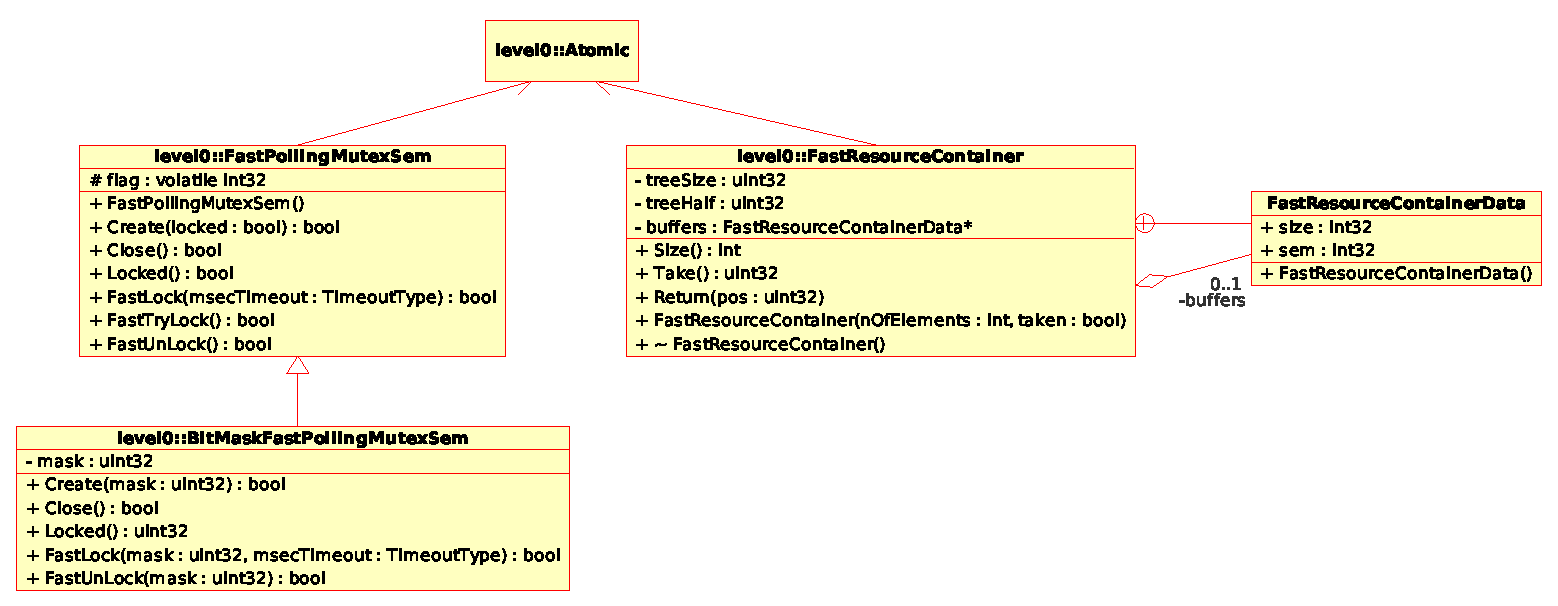
\includegraphics[width=\textwidth]{level0/level0-IPC-Fast.eps}
  \caption{BaseLib Level0 IPC Fast classes}
  \label{f:level0:ipc-fast}
 \end{center}
\end{figure}

Figure \ref{f:level0:ipc-fast} depict spinlock classes in this section (other classes previously anlized are also present: \texttt{Atomic}):

\begin{itemize}
 \item FastPollingMutexSem
 \item BitMaskFastPollingMutexSem
 \item FastResourceContainer
\end{itemize}




\subsubsection{FastPollingMutexSem}
\texttt{[FastPollingMutexSem]}\\
Class \texttt{FastPollingMutexSem} implements a spinlock using atomic test and set operations. Such class can be lock and unlock using also a timeout that is calculated using the \texttt{HRT} class.\\


API naming is quite similar to the \texttt{MutexSem} implementation. The interface is quite simple. \texttt{Create} method initializes the semaphore and reads it; \texttt{Close} undo semaphore initialization. 

The ambiguous named method \texttt{Locked} returns the status of the semaphore.

In this case ``fast'' functions have a meaning infact are the core of this class. \texttt{FastLock} poll the state of the mutex variable at a rate of a one milli seconds until \texttt{msecTimeout} is expired; this is a user space implementation of a spinlock; \texttt{FastTryLock} basically try to achieve the lock one time without waiting; \texttt{FastUnLock} unlock the mutex.

\begin{lstlisting}[
extendedchars=true,%
basicstyle=\fontfamily{pcr}\fontseries{m}\selectfont\footnotesize, %
stepnumber=1,%
numberstyle=\tiny,%
keywordstyle=\footnotesize\tt ,%
language=C++]
public:
   bool Create(bool locked = False);
   bool Close();

   inline bool Locked();

   inline bool FastLock(TimeoutType msecTimeout=TTInfiniteWait);
   inline bool FastTryLock();
   inline bool FastUnLock(void);
\end{lstlisting}

This class is suitable for multiprocessor systems and is the best choice when no OS interference is needed.



\subsubsection{BitMaskFastPollingMutexSem}
\texttt{[BitMaskFastPollingMutexSem.h]}\\
This structure group 32 mutexes, the locked/unlocked state of those mutexes can not be changed interleavedly so a mutex exist to control the access to the shared resource that is the \texttt{uint32} attribute holding the state of all mutexes. This class subclasses the \texttt{FastPollingMutexSem} class requiring it to provide access control to the shared 32 mutex's states.\\


The \texttt{mask} argument in the following methods is required to identify which of the 32 mutexes we want deal with.

\begin{lstlisting}[
extendedchars=true,%
basicstyle=\fontfamily{pcr}\fontseries{m}\selectfont\footnotesize, %
stepnumber=1,%
numberstyle=\tiny,%
keywordstyle=\footnotesize\tt ,%
language=C++]
private:
    uint32 mask;
public:
   bool Create(uint32 mask=0);
   bool Close();

   inline uint32 Locked();

   inline bool FastLock(uint32 mask,TimeoutType msecTimeout=TTInfiniteWait);
   inline bool FastUnLock(uint32 mask);
\end{lstlisting}



\subsubsection{FastResourceContainer}
\texttt{[FastResourceContainer.h]}\\
The class \texttt{FastResourceContainer} is basically an array data structure that if associated to a pool of resource give you the state of each resource. This means that let's for example that you have a pool of N \texttt{int}s in an array that goes from index 0 to index N-1, so you need one of them but without taking care of the index; this could be the condition when multiple entity concurrently need the same type of resource. In this situation you want to ask for a resource and take it without waiting and whitout OS's intervention.
A \texttt{FastResourceContainer} is the key in this situation, it doesn't allocate space buffer for you but can take care of which element of your pool are in use and which are not in use, answering for resource in a time O(n log n). If the pool has no resource your request simply fails. An example application will follow. \\


This mechanism can be imaged as a counting semaphore, independent from the OS because relies only on atomic hardware operations, so can be used between processes, threads, interrupt context on different processors in the mean time returning always immediate (without delay) in a bounded time (real time). \\


The class relay on a nested defined class \texttt{FastResourceContainerData} that take account of the usage state of each controlled resource.
The constructor take care on how many resource do you want to control, \texttt{Size} return the same number; \texttt{Take} return the index of a free resource and \texttt{Return} let you returning a resource index to the system.

\begin{lstlisting}[
extendedchars=true,%
basicstyle=\fontfamily{pcr}\fontseries{m}\selectfont\footnotesize, %
stepnumber=1,%
numberstyle=\tiny,%
keywordstyle=\footnotesize\tt ,%
language=C++]
private:
   uint32 treeSize;
   uint32 treeHalf;

   FastResourceContainerData* buffers;
public:
   FastResourceContainer(int nOfElements,bool taken=False);
   virtual ~FastResourceContainer();

   inline int Size();

   inline uint32 Take();
   inline void Return(uint32 pos);
\end{lstlisting}

Then follow an illustrative example on how to use a \texttt{FastResourceContainer}. In this example we create a buffer memory pool, this buffer memory pool can be used in multiprocessor and in multiple context in the same time thanks to the \texttt{FastResourceContainer}.

\begin{lstlisting}[
extendedchars=true,%
basicstyle=\fontfamily{pcr}\fontseries{m}\selectfont\footnotesize, %
stepnumber=1,%
numberstyle=\tiny,%
keywordstyle=\footnotesize\tt ,%
language=C++]
class DynamicPool: protected FastResourceContainer {
   int size;
   char* ptrBuffer;
public:
   DynamicPool(unsigned int size, int nOfElements, bool taken=False) {
      if (!(size)) size = 1;
      FastResourceContainer(nOfElements, taken);
      ptrBuffer = new char[size*nOfElements];
      this->size = size;
   }
   virtual ~DynamicPool() {
      if (ptrBuffer) delete ptrBuffer;
   }
   int alloc(char*& address) {
      int handle = (int)Take();
      if (handle == -1) return -1;
      address = ptrBuffer + (char*)(size*handle);
      return handle;
   }
   bool free(int handle) {
      return Return((unsigned int)handle);
   }
};
\end{lstlisting}



\subsection{Design Notes}

The \textit{SemNameDataBase} is used in every installation where the OS's libraies doesn't supply the named semaphore abstraction.
Some problems with semaphores are stated in the text; one big implementation problem is the static casting. Static casting is usually a bad programming choice, lets take a non skilled programmer: it pass to a function a wrong object without the right attributes but we are using those attributes in the function! What happens? Bugs, bugs and bugs...\\


SemPurger
The \texttt{Found} method is not a well designed method: the class is not associated to a \texttt{LinkedList} so there is no way to know to which sublist the \texttt{found} attribute's value refer.
A bad implementation choice in those classes is the interface of the \texttt{Test} method: is not really the interface but the code, inside the code there is a static cast of the \texttt{data} argument to \texttt{SemInfoDataBits} a \textit{dynamic cast} was probably a better choice to be sure to have some consistency checks in the code. \\


\texttt{SemCore} that probably can be renamed in something like \texttt{InterfaceSem}; such class is quite useless right now holding only an handle to an OS's entity. The usage count in the \textit{SemNameDataBase} is not currently checked against deletion of a semaphore. \\


The ambiguous named method \texttt{FastPollingMutexSem::Locked} returns the status of the semaphore, a better choice for this name could be \texttt{FastPollingMutexSem::isLocked} (?).



\section{Network}
\begin{figure}[h!]
  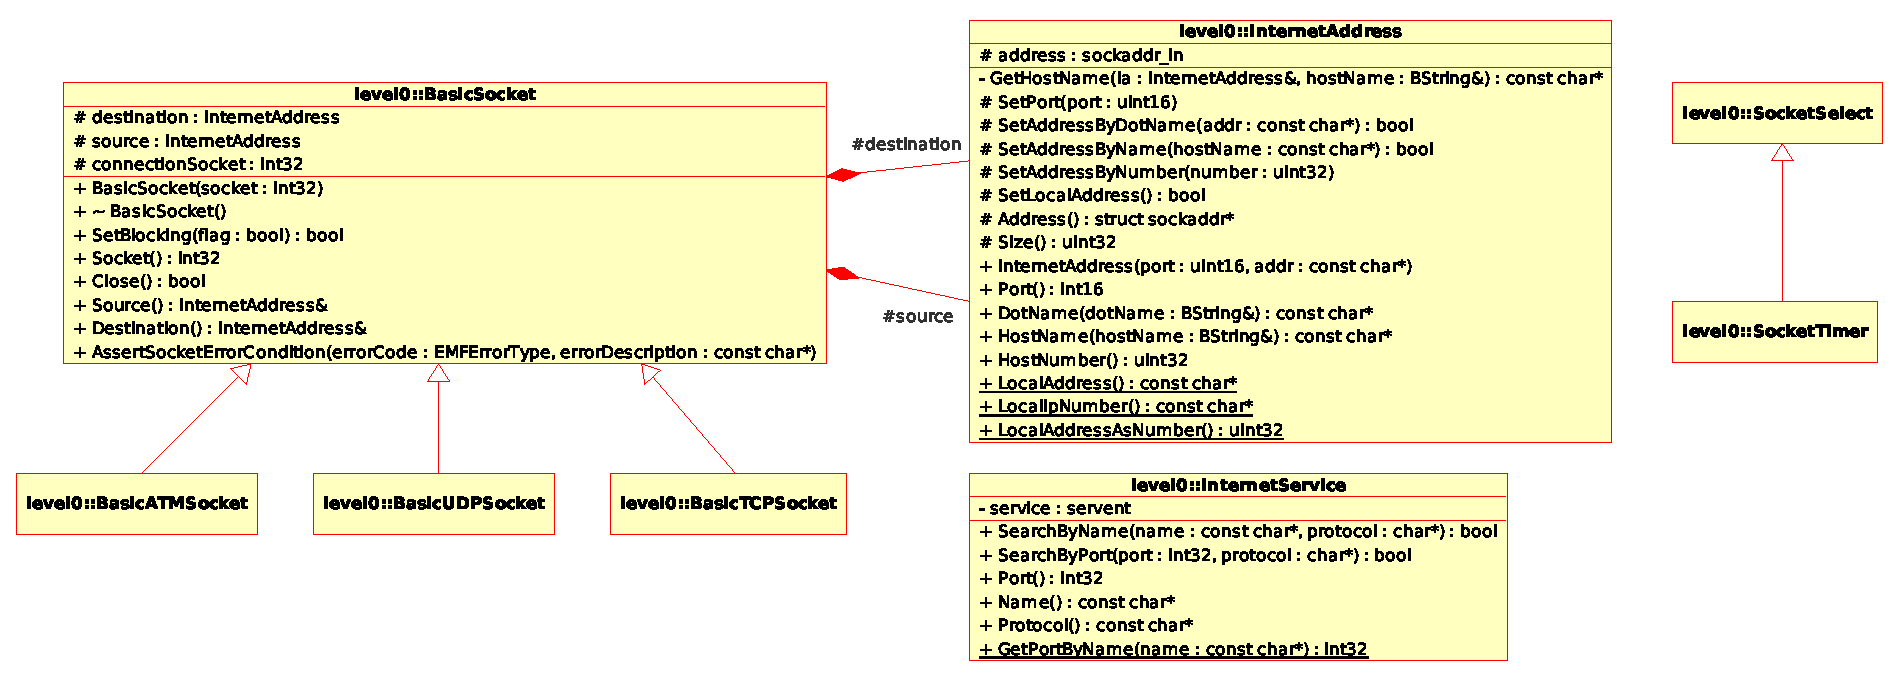
\includegraphics[width=\textwidth]{level0/level0-network.eps}
 \caption{BaseLib Level0 network classes}
 \label{f:level0:network}
\end{figure}

Network classes (Figure \ref{f:level0:network}) at these level inherit from the class \texttt{BasicSocket}. The class \texttt{BasicSocket} treat each source and destination address as a \texttt{InternetAddress} structure. We will start examining such class. \\

Classes in this section:
\begin{itemize}
 \item InternetAddress
 \item InternetService
 \item BasicSocket
 \item BasicATMSocket
 \item BasicTCPSocket
 \item BasicUDPSocket
 \item SocketSelect
 \item SocketTimer
\end{itemize}



\subsubsection{InternetAddress}
\texttt{[InternetAddress.h, InternetAddress.cpp]}\\
Class \texttt{InternetAddress} basically hold the full Internet Protocol version 4.0 (IPv4.0) address (i.e. the IP address and the port number). Right now IPv6.0 is not supported. The class is based on a protected UNIX \texttt{sockaddr\_in} structure.

\begin{lstlisting}[
extendedchars=true,%
basicstyle=\fontfamily{pcr}\fontseries{m}\selectfont\footnotesize, %
stepnumber=1,%
numberstyle=\tiny,%
keywordstyle=\footnotesize\tt ,%
language=C++]
protected:
   sockaddr_in address;
\end{lstlisting}

Setting the IP address is achieved by different functions letting friend classes and subclasses set it by dotted number notation (i.e. 192.168.1.2), name (i.e www.google.co.uk), by 32bit number (i.e. usually in hexadecimal format) and automatically, using the localhost IP; also the port number is not publically settable.

\begin{lstlisting}[
extendedchars=true,%
basicstyle=\fontfamily{pcr}\fontseries{m}\selectfont\footnotesize, %
stepnumber=1,%
numberstyle=\tiny,%
keywordstyle=\footnotesize\tt ,%
language=C++]
protected:
   bool SetAddressByDotName(const char* addr);
   bool SetAddressByName(const char* hostName);
   void SetAddressByNumber(uint32 number);
   bool SetLocalAddress();

   void SetPort(uint16 port);
\end{lstlisting}

Next code lines completes class's interface; the constructor take the port number and the IP in a suitable format to be given in input at the  \texttt{inet\_addr} POSIX API; such function use the numbers-and-dots notation. Public methods let the user only get the IP in different formats, public methods don't allow a user to modify the IP and port number the class holds.

\begin{lstlisting}[
extendedchars=true,%
basicstyle=\fontfamily{pcr}\fontseries{m}\selectfont\footnotesize, %
stepnumber=1,%
numberstyle=\tiny,%
keywordstyle=\footnotesize\tt ,%
language=C++]
   struct sockaddr *Address();
   uint32 Size();
public:
   InternetAddress(uint16 port=0,const char* addr=NULL);

   int16 Port();
   uint32 HostNumber();
   static const char* LocalAddress();
   static const char* LocalIpNumber();
   static uint32 LocalAddressAsNumber();
\end{lstlisting}

The last two functions use the special \texttt{BString} buffer class also defined in directory \textit{level0}. The function \texttt{DotName}
returns the host name in numbers-and-dots notation the returned \texttt{const char*} is a pointer to the \texttt{BString} buffer; the function \texttt{HostName} returns the host name (as a pointer to the BString buffer) by querying the name server, NULL means failure.

\begin{lstlisting}[
extendedchars=true,%
basicstyle=\fontfamily{pcr}\fontseries{m}\selectfont\footnotesize, %
stepnumber=1,%
numberstyle=\tiny,%
keywordstyle=\footnotesize\tt ,%
language=C++]
   const char* DotName(BString &dotName);
   const char* HostName(BString &hostName);
\end{lstlisting}



\subsubsection{BasicSocket}
\texttt{[BasicSocket.h, BasicSocket.cpp]}\\
This class implements generic socket functions. The socket abstraction require to specify an \texttt{InternetAddress} destination and a source. Socket is an abstraction that comes from POSIX standars; using the \textit{libc} library, each opened socket, like each opened file in a program, has associated a unique integer.

\begin{lstlisting}[
extendedchars=true,%
basicstyle=\fontfamily{pcr}\fontseries{m}\selectfont\footnotesize, %
stepnumber=1,%
numberstyle=\tiny,%
keywordstyle=\footnotesize\tt ,%
language=C++]
protected:
   InternetAddress destination;
   InternetAddress source;
   int32           connectionSocket;
\end{lstlisting}

This class is an abstract class defining only the concept behind Sockets: it defines three basic attributes but doesn't implements methods to set or get those attributes, this is not absolutely true but for example you can get the \texttt{destination} and \texttt{source} address but not set. The constructor require a socket identifier, so this class doesn't create a socket for you, is the user that have to first create a socket and than associate a classes to such socket.

\begin{lstlisting}[
extendedchars=true,%
basicstyle=\fontfamily{pcr}\fontseries{m}\selectfont\footnotesize, %
stepnumber=1,%
numberstyle=\tiny,%
keywordstyle=\footnotesize\tt ,%
language=C++]
public:
   BasicSocket(int32 socket = 0);

   bool SetBlocking(bool flag);
   int32 Socket();
   bool Close();
   InternetAddress& Source();
   InternetAddress& Destination();

   void AssertSocketErrorCondition(EMFErrorType errorCode,const char* errorDescription=NULL,...);
   void AssertSocketErrorCondition(EMFErrorType errorCode,const char* errorDescription=NULL,...);
\end{lstlisting}

Last two lines implement error handling for the first time. The enumerated type \texttt{EMFErrorType} follows in the section Exceptions in this chapter; \texttt{errorCode} is a number identifying the type of error not the dangerous level of the error.



\subsubsection{BasicATMSocket}
\texttt{[BasicATMSocket.h, BasicATMSocket.cpp]}\\
This class is one of the three subclasses of the \texttt{BasicSocket} class. Basically it adds the support to ATM socket at AAL5 protocol. An ATM network is not socket oriented but it relay on channels (Virtual Circuits). Unix developer try to uniformly this kind of network letting ATM network users using the same socket abstraction used for connection oriented protocols.

The most important information regarding a Virtual Circuit is the Virtual Circuit Index (VCI).

\begin{lstlisting}[
extendedchars=true,%
basicstyle=\fontfamily{pcr}\fontseries{m}\selectfont\footnotesize, %
stepnumber=1,%
numberstyle=\tiny,%
keywordstyle=\footnotesize\tt ,%
language=C++]
protected:
   uint32 VCI;
\end{lstlisting}

This code use the POSIX interface to write and read to an ATM network card. Core functions to read or write are private and are declared as follow. This solution is adopted to let a set of friends function calling the methods have access to protected attributes of \texttt{InternetAddress}. A C interface that use the object is given.

\begin{lstlisting}[
extendedchars=true,%
basicstyle=\fontfamily{pcr}\fontseries{m}\selectfont\footnotesize, %
stepnumber=1,%
numberstyle=\tiny,%
keywordstyle=\footnotesize\tt ,%
language=C++]
private:
   bool _Read(const void* buffer,uint32& size,TimeoutType msecTimeout);
   bool _Write(const void* buffer,uint32& size,TimeoutType msecTimeout);
\end{lstlisting}

Like a \texttt{BasicSocket} the constructor doesn't create a socket but it is the user that must supply a newly created socket for the constructor. Using the \texttt{Open} method it is possible to open a new ATM socket without passing it via the constructor, \texttt{SetVCI} and \texttt{GetVCI} let's setting and getting the Virtual Channel Index (a number).

The \texttt{Read} and \texttt{Write} function reads and writes a block of data, \texttt{size} is the maximum size in bytes of the required transfer for a write operation; during a read \texttt{size} holds first the maximum buffer size and after the read the readed size in bytes. Timeout is currently not supported.

\begin{lstlisting}[
extendedchars=true,%
basicstyle=\fontfamily{pcr}\fontseries{m}\selectfont\footnotesize, %
stepnumber=1,%
numberstyle=\tiny,%
keywordstyle=\footnotesize\tt ,%
language=C++]
public:
   BasicATMSocket(int32 socket);

   bool Open();
   inline bool Read(void* buffer, uint32& size, TimeoutType msecTimeout=TTDefault);
   inline bool Write(const void* buffer, uint32& size, TimeoutType msecTimeout=TTDefault);
   inline bool SetVCI(int32 VCI);
   inline uint32 GetVCI();
\end{lstlisting}

To use an ATM oriented channel using such class interface it is necessary to follow those steps, in that order:
\begin{enumerate}
 \item create a brand new \texttt{BasicATMSocket} object;
 \item call method \texttt{Open} on the object;
 \item call method \texttt{SetVCI} on the object;
 \item now it is possible to read and wirte on the object.
\end{enumerate}



\subsubsection{BasicTCPSocket}
\texttt{[BasicTCPSocket.h]}\\
Implements general TCP/IP stream-sockets. All methods implemented in this class are public, no private attribute or method. There are three IO functions: one to write on the stream and two to read from, the second, \texttt{Peek} doesn't consume what it reads.

\begin{lstlisting}[
extendedchars=true,%
basicstyle=\fontfamily{pcr}\fontseries{m}\selectfont\footnotesize, %
stepnumber=1,%
numberstyle=\tiny,%
keywordstyle=\footnotesize\tt ,%
language=C++]
public:
   bool BasicWrite(const void* buffer, uint32& size);
   bool BasicRead(void* buffer, uint32& size);
   bool Peek(void* buffer, uint32& size);
\end{lstlisting}

The constructor take as an argument a socket. If you doesn't want to supply a socket the function \texttt{Open} create one for you. \texttt{Listen} functions bind the socket on a given port number for incoming connections, the function \texttt{WaitConnection} return \texttt{BasicTCPSocket*} on newly estabilished connection on the binded socket.
\texttt{Connect} functions let the user connect to some other remote or local sockets.

\begin{lstlisting}[
extendedchars=true,%
basicstyle=\fontfamily{pcr}\fontseries{m}\selectfont\footnotesize, %
stepnumber=1,%
numberstyle=\tiny,%
keywordstyle=\footnotesize\tt ,%
language=C++]
   BasicTCPSocket(int32 socket = 0);
   bool Open();

   bool Listen(int port,int maxConnections=1);
   bool Listen(char *serviceName,int maxConnections=1);
   BasicTCPSocket* WaitConnection(TimeoutType msecTimeout=TTInfiniteWait,
      BasicTCPSocket* client=NULL);

   bool Connect(const char* address,int port,TimeoutType msecTimeout=TTInfiniteWait);
   bool Connect(const char* address,const char* serviceName,
      TimeoutType msecTimeout=TTInfiniteWait);
   bool IsConnected();
\end{lstlisting}

This interface permit to specify ports as a number or as a service name (string) this is achieved using the \texttt{InternetService::GetPortByName} facility. The \texttt{InternetService} interface is reported here:

\begin{lstlisting}[
extendedchars=true,%
basicstyle=\fontfamily{pcr}\fontseries{m}\selectfont\footnotesize, %
stepnumber=1,%
numberstyle=\tiny,%
keywordstyle=\footnotesize\tt ,%
language=C++]
class InternetService {
   servent service;
public:
   bool SearchByName(const char* name,char* protocol=NULL);
   bool SearchByPort(int32 port,char* protocol=NULL);
   int32 Port();
   const char* Name();
   const char* Protocol();
   static int32 GetPortByName(const char* name);
};
\end{lstlisting}



\subsubsection{BasicUDPSocket}
\texttt{[BasicUDPSocket.h]}\\
Implements a general UDP/IP socket. UDP protocol is connectionless and so differently from TCP doesn't need a connection, the \texttt{BasicUDPSocket} class implements also the \texttt{Connect} function that is used to select the destination of the next sends; infact using the IO function below is not possible to choose a destination address. Every message received on the selected UDP port is received.

\begin{lstlisting}[
extendedchars=true,%
basicstyle=\fontfamily{pcr}\fontseries{m}\selectfont\footnotesize, %
stepnumber=1,%
numberstyle=\tiny,%
keywordstyle=\footnotesize\tt ,%
language=C++]
public:
   bool BasicRead(void* buffer, uint32& size);
   bool BasicWrite(const void* buffer, uint32& size);
\end{lstlisting}

As usual the constructor let you create an object using a previous opened UDP socket or create a brand new socket with the \texttt{Open} method.

\begin{lstlisting}[
extendedchars=true,%
basicstyle=\fontfamily{pcr}\fontseries{m}\selectfont\footnotesize, %
stepnumber=1,%
numberstyle=\tiny,%
keywordstyle=\footnotesize\tt ,%
language=C++]
   BasicUDPSocket(int32 socket = 0);
   bool Open();

   bool Listen(int port,int maxConnections=1);
   bool Connect(const char *address,int port);
   bool Connect(InternetAddress &dest);
\end{lstlisting}



\subsubsection{SocketSelect}
\texttt{[SocketSelect.h]}\\
This class provide a wrapper to the \texttt{select} \textit{libc} function allowing the synchronization of a group of sockets. This stuff can only select sockets from a single source type, is not allowed to mix ATM and UDP on NT platforms.

\begin{lstlisting}[
extendedchars=true,%
basicstyle=\fontfamily{pcr}\fontseries{m}\selectfont\footnotesize, %
stepnumber=1,%
numberstyle=\tiny,%
keywordstyle=\footnotesize\tt ,%
language=C++]
protected:
   fd_set readFDS;
   fd_set writeFDS;
   fd_set exceptFDS;
   fd_set readFDS_done;
   fd_set writeFDS_done;
   fd_set exceptFDS_done;
   int32 readySockets;

public:
   SocketSelect();

   void Reset();
   void AddWaitOnWriteReady(BasicSocket* s);
   void DeleteWaitOnWriteReady(BasicSocket* s);
   void AddWaitOnReadReady(BasicSocket* s);
   void DeleteWaitOnReadReady(BasicSocket* s);
   void AddWaitOnExceptReady(BasicSocket* s);
   void DeleteWaitOnExceptReady(BasicSocket* s);

   bool Wait(TimeoutType msecTimeout=TTInfiniteWait);
   bool WaitRead(TimeoutType msecTimeout=TTInfiniteWait);
   bool WaitWrite(TimeoutType msecTimeout=TTInfiniteWait);
   bool WaitExcept(TimeoutType msecTimeout=TTInfiniteWait);

   int32 ReadySockets();
   bool CheckRead(BasicSocket* s);
   bool CheckWrite(BasicSocket* s);
   bool CheckExcept(BasicSocket* s);
   fd_set& ReadFDS();
   fd_set& WriteFDS();
   fd_set& ExceptFDS();
\end{lstlisting}



\subsubsection{SocketTimer}
\texttt{[SocketTimer.h]}\\
To simplify some use of select; this is a tool to specify a maximum wait on socket actions. The interface is quite simple. The most important thing is the time attribute \texttt{timeWait} that model the time to wait in a timeout operation.
It is possible to wait for a \textit{read} or \textit{write} operation.

\begin{lstlisting}[
extendedchars=true,%
basicstyle=\fontfamily{pcr}\fontseries{m}\selectfont\footnotesize, %
stepnumber=1,%
numberstyle=\tiny,%
keywordstyle=\footnotesize\tt ,%
language=C++]
private:
   timeval timeWait;

public:
   void SetMsecTimeout(TimeoutType msecTimeout=TTInfiniteWait);
   bool WaitRead();
   bool WaitWrite();
   uint32 MSecTimeout();
\end{lstlisting}



\subsection{Design Notes}

Sockets are a powerfull abstraction due to UNIX operating system. The construction adopted here is quite general and is fully compatible with many operating systems on the market. \\


Probably further code to support newer protocol like IPv6.0 is needed in the future. The class diagram using the class developed require that all the system relay on IP, that is not true for ATM networks, it lacks some generality. \\


Too many code inlining is not ever a good design choice: systems with low memory constraints will became fast a difficult target to support. Code inlining produce many copy of the same code in the library.\\



\section{Files, Streams}
This section groups togheter two basic concepts: files and streams. For each concepts there is a subsection. There are only few classes involved in this group.
If you see Files and Streams implementations you can note that the interface is quite similar between \texttt{BasicFile} and \texttt{StreamInterface}.



\subsection{Files}
Files abstraction come from UNIX OSes and are nowadays the principal abstraction for data storage. BaseLib's file classes are depicted in Figure \ref{f:level0:file}; there are only two classes, without any link, as listed below:
\begin{itemize}
 \item BasicFile
 \item BasicConsole
\end{itemize}

\begin{figure}[h!]
 \begin{center}
  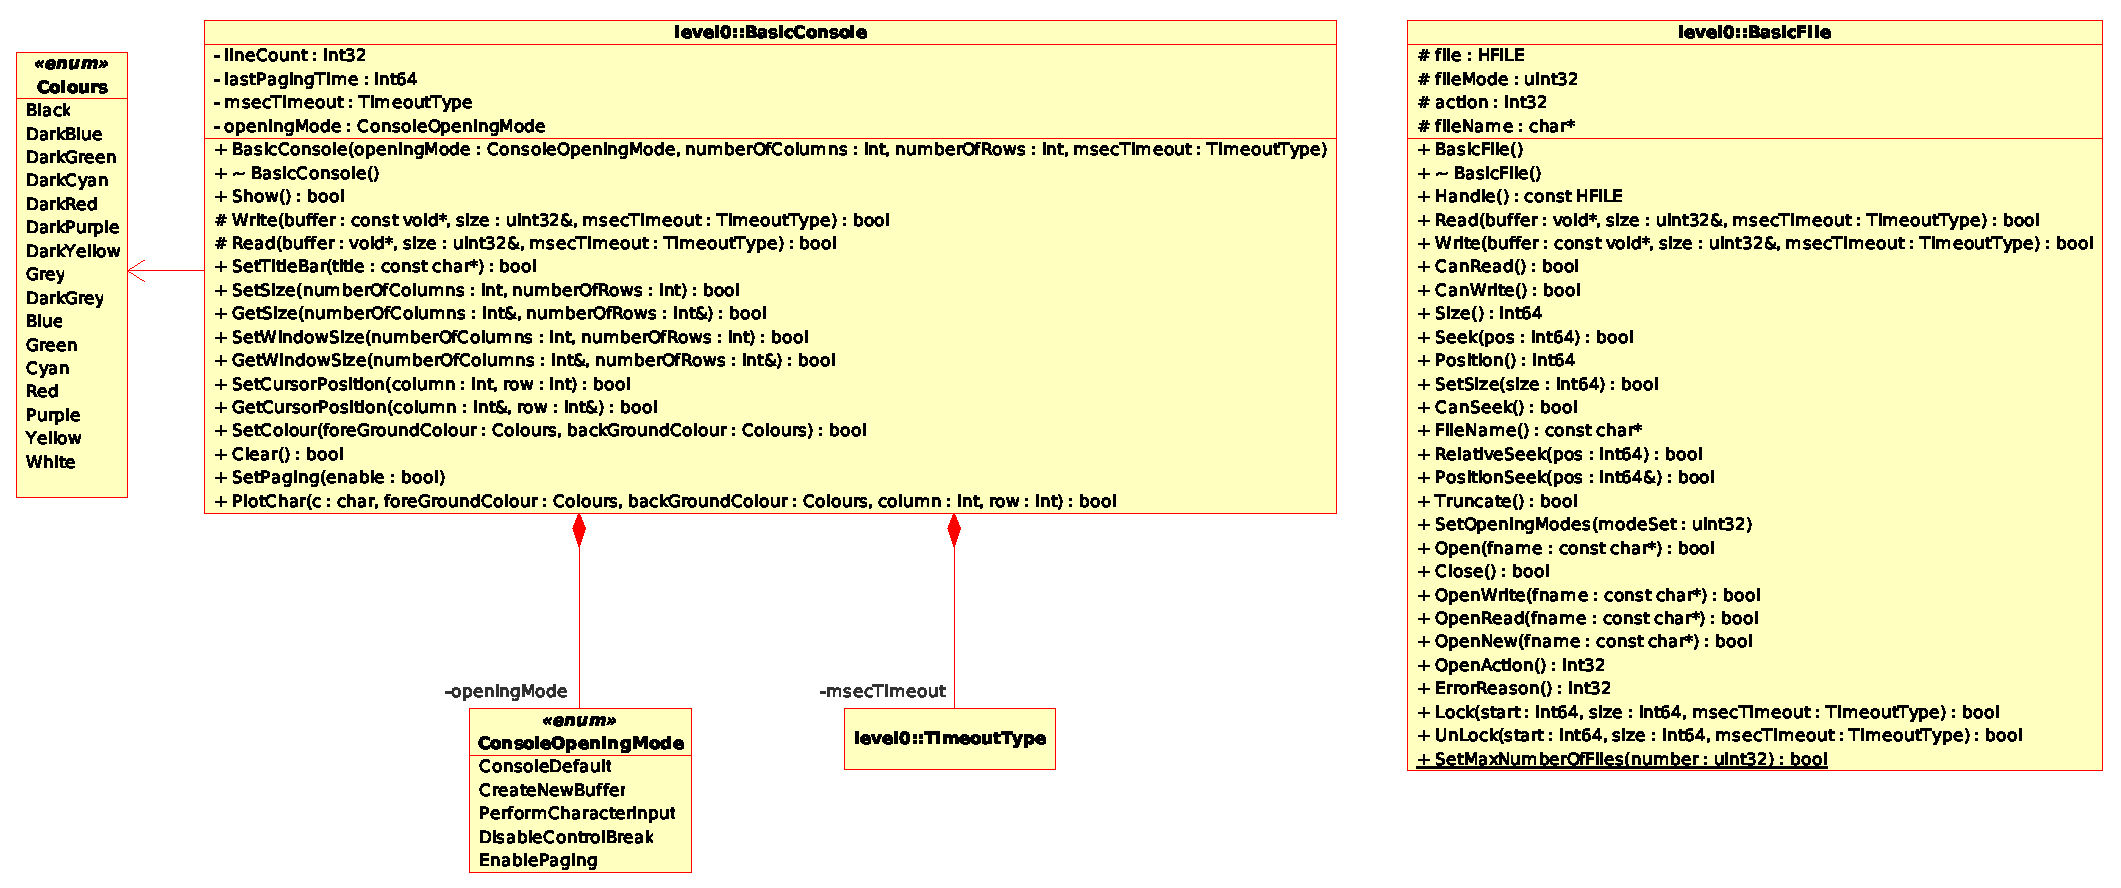
\includegraphics[width=\textwidth]{level0/level0-file.eps}
  \caption{BaseLib Level0 file classes}
  \label{f:level0:file}
 \end{center}
\end{figure}

Classes methods are quite similar, this is why they are grouped together, a Console or better a terminal, is in UNIX treated as a file with a more special interface support to terminal (see \texttt{man termios}). Infact during the past there were a great use of serial link and a serial link let computer dial togheter, a serial link in a UNIX system is a file and so a serial device is a file ( as an example \texttt{/dev/ttys0}) serial link has some special character (or set of it) that let the user treat it as a terminal so the UNIX developer introduced those special function as extended functions of a file abstraction. Infact in UNIX a Console can also be locked but in BaseLib no.



\subsubsection{BasicFile}
\texttt{[BasicFile.h, BasicFile.cpp]}\\
The \texttt{BasicFile} class is istantiated per opened file the basic information carried from the class is a \texttt{HFILE} handle to the file, a mode mask that can be queried to know if the file was opened in write or read only mode (\texttt{fileMode}), an \texttt{int32} attribute (\texttt{action)} used to hold an error code in case of failure and the file name (\texttt{fileName}).

\begin{lstlisting}[
extendedchars=true,%
basicstyle=\fontfamily{pcr}\fontseries{m}\selectfont\footnotesize, %
stepnumber=1,%
numberstyle=\tiny,%
keywordstyle=\footnotesize\tt ,%
language=C++]
protected:
   HFILE file;
   uint32 fileMode;
   int32 action;
   char* fileName;
\end{lstlisting}

There is only one protected method \texttt{SetFileName} that let the developer of subclasses to change the file's name. The class constructor doesn't require any parameters.\\


Basic \textit{get} methods are \texttt{Handle} that return the OS related file handle (an integer in UNIX); \texttt{FileName} return the name of the file and \texttt{Size} return the size of the file object. The method \texttt{SetSize} lets you set the file size by either truncating or extending the file size. The only static method, \texttt{SetMaxNumberOfFiles} try to set a Operating System wide parameter of the maximum number of files opened in the system, in VxWorks it simply return \texttt{true}.

\begin{lstlisting}[
extendedchars=true,%
basicstyle=\fontfamily{pcr}\fontseries{m}\selectfont\footnotesize, %
stepnumber=1,%
numberstyle=\tiny,%
keywordstyle=\footnotesize\tt ,%
language=C++]
   void SetFileName(const char* name);
public:
   const HFILE Handle();
   inline const char* FileName();

   inline int64 Size();
   inline bool SetSize(int64 size);

   static inline bool SetMaxNumberOfFiles(uint32 number);
\end{lstlisting}

Before opening a file the first action to do is to set the file opening modes with the \texttt{SetOpeningModes}, opening modes are listed in the firt 50's row of the file \textit{level0/BasicFile.h}. Then it is possible to open a file with the method \texttt{Open}. To avoid the burden of making two calls it is possible to use the methods \texttt{OpenWrite} \texttt{OpenRead} \texttt{OpenNew} to open for write, open read only and create a file. If during an open operation happen something unexpected it's possible to query about what happens with the \texttt{OpenAction} and \texttt{ErrorReason} methods.

\begin{lstlisting}[
extendedchars=true,%
basicstyle=\fontfamily{pcr}\fontseries{m}\selectfont\footnotesize, %
stepnumber=1,%
numberstyle=\tiny,%
keywordstyle=\footnotesize\tt ,%
language=C++]
   inline void SetOpeningModes(uint32 modeSet);
   bool Open(const char *fname,...);
   inline bool Close();

   bool OpenWrite(const char *fname,...);
   bool OpenRead(const char *fname,...);
   bool OpenNew(const char *fname,...);

   inline int32 OpenAction();
   int32 ErrorReason();
\end{lstlisting}

The \texttt{Read} and \texttt{Write} operation have a timeout to stop blocking the caller processor. The functions have the same interface, the size in each case is readed and written so its an in/out argument. Query methods \texttt{CanRead} and \texttt{CanWrite} parse the attribute \texttt{fileMode} to understand with which options the file was opened. There is no way to understand if the file was just opened or newer opened.

\begin{lstlisting}[
extendedchars=true,%
basicstyle=\fontfamily{pcr}\fontseries{m}\selectfont\footnotesize, %
stepnumber=1,%
numberstyle=\tiny,%
keywordstyle=\footnotesize\tt ,%
language=C++]
   inline bool Read(void* buffer, uint32& size, TimeoutType msecTimeout=TTDefault);
   inline bool Write(const void* buffer, uint32& size, TimeoutType msecTimeout=TTDefault);
   inline bool CanRead();
   inline bool CanWrite();
\end{lstlisting}

For random file access BaseLib supplies \texttt{Position} method to know the current file position; with the \texttt{CanSeek} method it possible to query regarding the capability of seeking a file (basically an OS's dependent task). Seeking a file is easily obtained using \texttt{Seek} to move to a specific absolute position (i.e. the position is expressed from the beginning of the file), \texttt{PositionSeek} method behave in the same way but the \texttt{pos} is an in/out argument; if you require to move to a relative position simply use \texttt{RelativeSeek}.\\


The method \texttt{Truncate} clip the file size to the current seek point (i.e. the current position). The last two function let the user lock and unlock to the application the access of the file region starting from \texttt{start} and \texttt{size} bytes long. If it was locked wait as much as timeout.

\begin{lstlisting}[
extendedchars=true,%
basicstyle=\fontfamily{pcr}\fontseries{m}\selectfont\footnotesize, %
stepnumber=1,%
numberstyle=\tiny,%
keywordstyle=\footnotesize\tt ,%
language=C++]
   inline int64 Position(void);

   inline bool CanSeek();
   inline bool Seek(int64 pos);
   inline bool PositionSeek(int64 &pos);
   inline bool RelativeSeek(int64 pos);

   inline bool Truncate();

   inline bool Lock(int64 start,int64 size,TimeoutType msecTimeout = TTInfiniteWait);
   inline bool UnLock(int64 start,int64 size,TimeoutType msecTimeout = TTInfiniteWait);
\end{lstlisting}



\subsubsection{BasicConsole}
\texttt{[BasicConsole.h, BasicConsole.cpp]}\\
As stated before a \textit{console} can be treated as a \textit{file} entity but in BaseLib are completely separated but there are some common methods with the same signature. An example of a console in Microsoft Windows$^{\copyright}$ is the Command Prompt in Linux and other UNIX systems you can experienced differents sort of consoles. \\


Attributes start with some OS's handle different from OS to OS, below are cut and pasted only Window's and Linux's handles. \texttt{lineCount} count how many lines since last paging and \texttt{lastPagingTime} how long since last paging; \texttt{msecTimeout} represents how long to wait when reading on the console, \texttt{openingMode} sets of flags describing the console status.

\begin{lstlisting}[
extendedchars=true,%
basicstyle=\fontfamily{pcr}\fontseries{m}\selectfont\footnotesize, %
stepnumber=1,%
numberstyle=\tiny,%
keywordstyle=\footnotesize\tt ,%
language=C++]
#if defined (_WIN32)
   HANDLE inputConsoleHandle;
   HANDLE outputConsoleHandle;
#elif defined (_LINUX)
   struct termio originalConsoleModes;
#endif
   int32 lineCount;
   int64 lastPagingTime;
   TimeoutType msecTimeout;
   ConsoleOpeningMode openingMode;
\end{lstlisting}

The constructor takes four arguments: the first is of type \texttt{ConsoleOpeningMode}, an \texttt{enum} (defined in \textit{level0/BasciConsole.h}) that defines how to open the console (can be an orred combination); the second and the third arguments define respectively the number of columns and rows of the opened console; the last argument is a timeout that update the attribute \texttt{msecTimeout}.
\texttt{Show} simply try to show the console; basically it call an OS's API.

Protected methods let a subclass to write and read to the console; only a subclass is able to make IO operations on a \texttt{BasicConsole} this require to extend a \texttt{BasicConsole} to have a real working \textit{console}.


\begin{lstlisting}[
extendedchars=true,%
basicstyle=\fontfamily{pcr}\fontseries{m}\selectfont\footnotesize, %
stepnumber=1,%
numberstyle=\tiny,%
keywordstyle=\footnotesize\tt ,%
language=C++]
public:
   BasicConsole(ConsoleOpeningMode openingMode=ConsoleDefault,
      int numberOfColumns=-1,
      int numberOfRows=-1,
      TimeoutType msecTimeout=TTInfiniteWait);
   virtual ~BasicConsole();

   inline bool Show();
protected:
   inline bool Write(const void* buffer,uint32& size,TimeoutType msecTimeout);
   inline bool Read(void* buffer,uint32& size,TimeoutType msecTimeout);
\end{lstlisting}

The following methods are oriented to graphical operating systems were a \textit{console} is usually displayed in a \textit{window}. The first method (\texttt{SetTitleBar}) infact lets you set the title bar text of a console window; \texttt{SetPaging} enable or disable paging in the console window; \texttt{SetColour} sets the font foreground and background colours. Take a look to the \texttt{enum Colours} in Figure \ref{f:level0:file} to see the currently available colours. \\


To set and retrieve the size of the \textit{console buffer} in columns and rows you must use \texttt{SetSize} and \texttt{GetSize}; to set and retrieve the size of the \textit{console window} in columns and rows there are \texttt{SetWindowSize} and \texttt{GetWindowSize}. Last couple of functions is full implemented only in Microsoft Windows$^{\copyright}$. Figure \ref{f:level0:console} explain the differences between the \textit{console window} and \textit{console buffer}.

\begin{figure}[h!]
 \begin{center}
  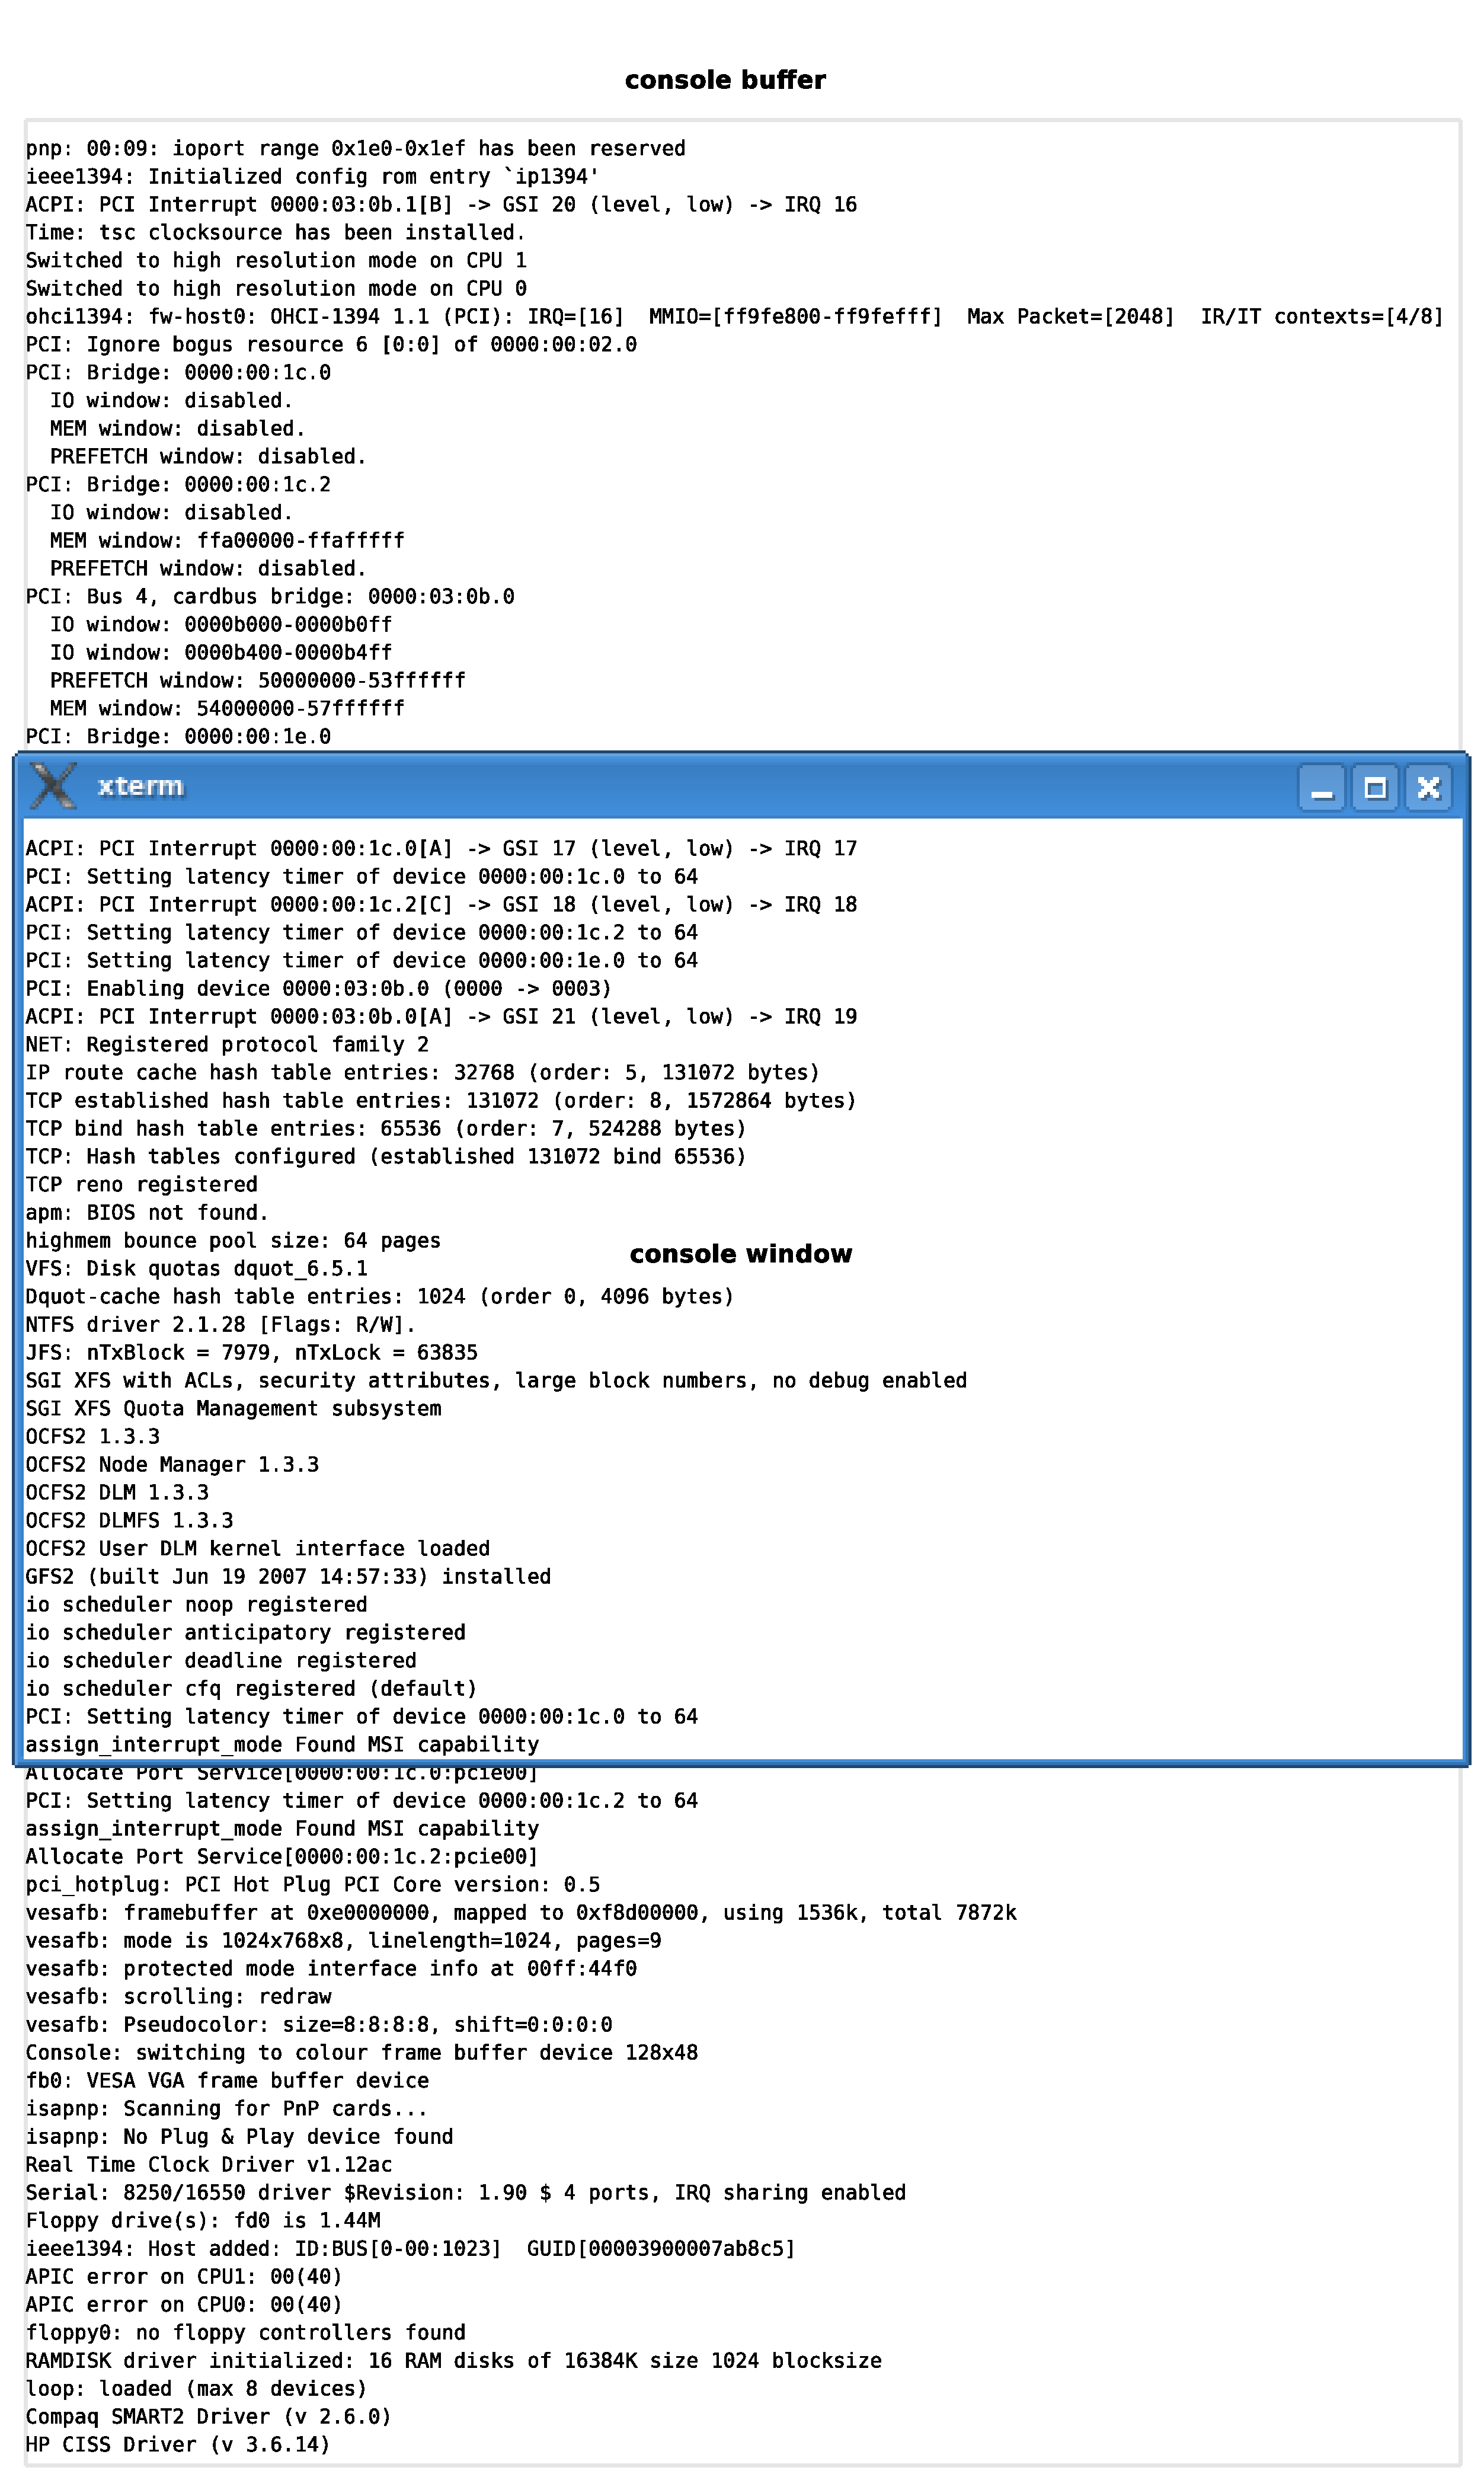
\includegraphics[width=0.49\textwidth]{level0/console.eps}
  \caption{BaseLib console scheme}
  \label{f:level0:console}
 \end{center}
\end{figure}

The method \texttt{SetCursorPosition} sets the position of the cursor in columns and rows; \texttt{GetCursorPosition} retrieve the cursor position. \texttt{Clear} clears the console's content. \texttt{PlotChar} write a single char on the console at a given position and with a given colour set.

\begin{lstlisting}[
extendedchars=true,%
basicstyle=\fontfamily{pcr}\fontseries{m}\selectfont\footnotesize, %
stepnumber=1,%
numberstyle=\tiny,%
keywordstyle=\footnotesize\tt ,%
language=C++]
public:
   inline bool SetTitleBar(const char* title);
   inline void SetPaging(bool enable);
   inline bool SetColour(Colours foreGroundColour,Colours backGroundColour);

   inline bool SetSize(int numberOfColumns,int numberOfRows);
   inline bool GetSize(int& numberOfColumns,int& numberOfRows);

   inline bool SetWindowSize(int numberOfColumns,int numberOfRows);
   inline bool GetWindowSize(int& numberOfColumns,int& numberOfRows);

   inline bool SetCursorPosition(int column, int row);
   inline bool GetCursorPosition(int& column,int& row);

   inline bool Clear();
   inline bool PlotChar(char c,
      Colours foreGroundColour,
      Colours backGroundColour,
      int column, int row);
\end{lstlisting}



\subsection{Streams}
The stream abstraction come from the Object Oriented Design work. C++ defines its standard streams, have a look at \texttt{iostream} and \texttt{fstream} but BaseLib redefine them. In this group of classes we explore the following classes (depicted in Figure \ref{f:level0:stream}):
\begin{itemize}
 \item StreamInterface
 \item PrintfStreamInterface
 \item CStream, CStreamNewBufferFN
\end{itemize}

\begin{figure}[h!]
 \begin{center}
  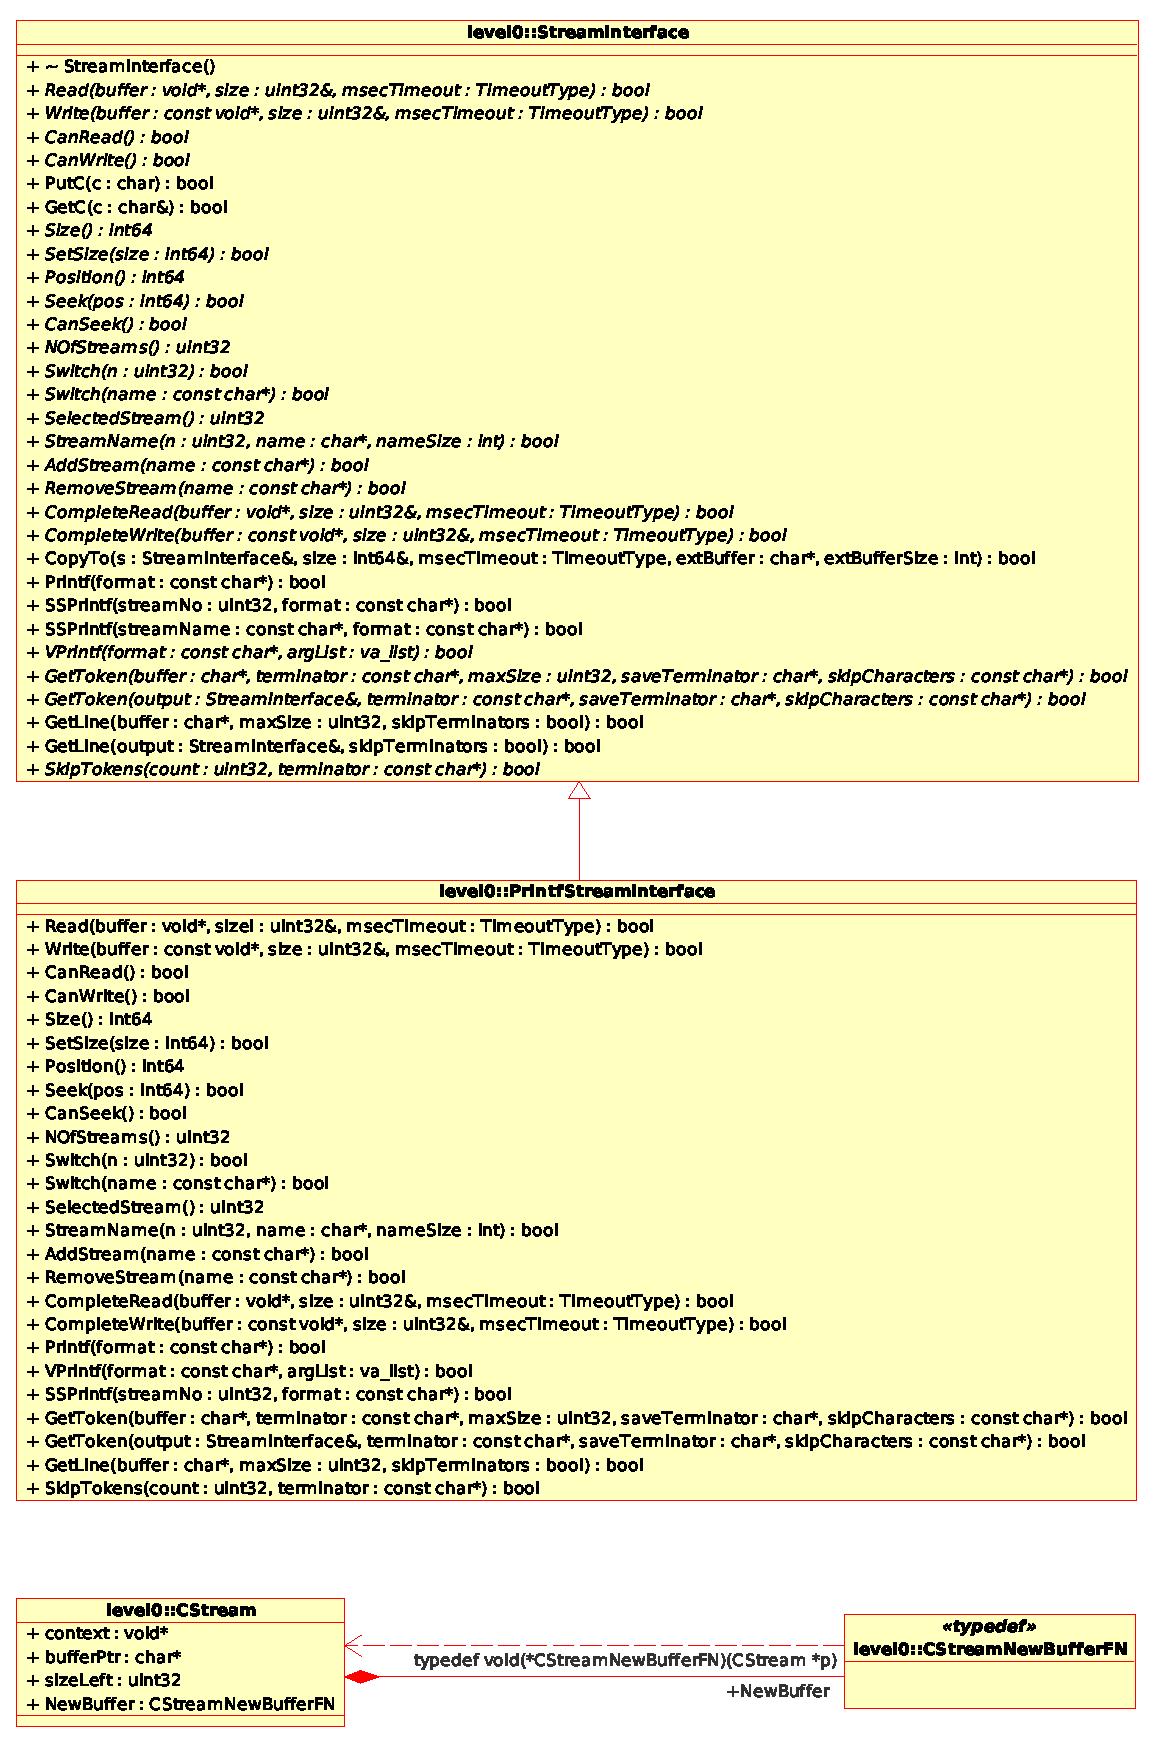
\includegraphics[width=0.57\textwidth]{level0/level0-stream.eps}
  \caption{BaseLib Level0 base stream classes}
  \label{f:level0:stream}
 \end{center}
\end{figure}



\subsubsection{StreamInterface}
\texttt{[StreamInterface.h, StreamInterface.cpp]}\\
The StreamInterface is really important: an entire BaseLib's Level is build on it. Such level focuses on streams defining the \texttt{Streamable} object on top of the \texttt{StreamInterface} that is abstract version. It is used to allow referring to streams at lower levels.
The class has many \textit{pure virtual} methods and a few inline methods so its an abstract C++ class.\\


The method \texttt{Read} reads data into \texttt{buffer} as much as \texttt{size} byte are written, actual size is returned in \texttt{size}; \texttt{msecTimeout} argument is how much the operation should last, timeout behaviour is class specific, i.e. sockets with blocking activated wait forever when \texttt{noWait} is used.
The method \texttt{Write} writes data from \texttt{buffer} to the stream as much as \texttt{size} byte are written, actual size is returned in \texttt{size}, \texttt{msecTimeout} is how much the operation should last; also here timeout behaviour is class specific.

Methods \texttt{CanRead} and \texttt{CanWrite} let you know about the capability to read or write on the stream. \texttt{PutC} implements a single character write operation, \texttt{GetC} implements single character read operation.

\begin{lstlisting}[
extendedchars=true,%
basicstyle=\fontfamily{pcr}\fontseries{m}\selectfont\footnotesize, %
stepnumber=1,%
numberstyle=\tiny,%
keywordstyle=\footnotesize\tt ,%
language=C++]
public:
   virtual bool Read(void* buffer,uint32& size,TimeoutType msecTimeout=TTDefault)=0;
   virtual bool Write(const void* buffer,uint32& size,TimeoutType msecTimeout=TTDefault)=0;

   virtual bool CanRead()=0;
   virtual bool CanWrite()=0;

   inline bool PutC(char c);
   inline bool GetC(char &c);
\end{lstlisting}

The method \texttt{Size} return the size of the stream and \texttt{SetSize} clip the stream size to a specified point (similar to \texttt{Truncate} method). \texttt{Position} returns current position, \texttt{Seek} moves within the file to an absolute location in the file and \texttt{CanSeek} let you query about the capability of seeking.

\begin{lstlisting}[
extendedchars=true,%
basicstyle=\fontfamily{pcr}\fontseries{m}\selectfont\footnotesize, %
stepnumber=1,%
numberstyle=\tiny,%
keywordstyle=\footnotesize\tt ,%
language=C++]
   virtual int64 Size()=0;
   virtual bool SetSize(int64 size)=0;

   virtual int64 Position(void)=0;
   virtual bool Seek(int64 pos)=0;
   virtual bool CanSeek()=0;
\end{lstlisting}

Following methods define a multiple streams interface, \texttt{NOfStreams} return how many streams are available, \texttt{Switch} select the stream to read from, switching may reset the stream to the start, the same method overloaded let the user \texttt{Switch} by name to another stream. \texttt{SelectedStream} return the index of the currently used stream, using \texttt{StreamName} it possible to retrieve also the stream name. Using \texttt{AddStream} you can add a new stream to write to, removing is possible with \texttt{RemoveStream}. Those functions used togheter lets manage streams registration and cancellation.

\begin{lstlisting}[
extendedchars=true,%
basicstyle=\fontfamily{pcr}\fontseries{m}\selectfont\footnotesize, %
stepnumber=1,%
numberstyle=\tiny,%
keywordstyle=\footnotesize\tt ,%
language=C++]
   virtual uint32 NOfStreams()=0;
   virtual bool Switch(uint32 n)=0;
   virtual bool Switch(const char* name)=0;
   virtual uint32 SelectedStream()=0;
   virtual bool StreamName(uint32 n,char* name,int nameSize)=0;
   virtual bool AddStream(const char* name)=0;
   virtual bool RemoveStream(const char* name)=0;
\end{lstlisting}

The method \texttt{CompleteRead} performs the job of a \texttt{Read} function but gurantees the completion; in case of failure \texttt{size} returns the actual data readed, \texttt{msecTimeout} is the total allowed wait time checked using \texttt{HRT}.
The method \texttt{CompleteWrite} performs the job of a the \texttt{Write} function but gurantees the completion; in case of failure \texttt{size} returns the actual data written, \texttt{msecTimeout} is the total allowed wait time checked using \texttt{HRT}.
\texttt{CopyTo} copies \texttt{size} bytes to the stream \texttt{s} it stops on \texttt{msecTimeout} or on an EOF, returns \texttt{True} on success or on reaching EOF (if \texttt{msecTimeout} is \texttt{TTInfiniteWait}) otherwise \texttt{False}.\\


\texttt{Printf} print a formatted string on the current selected stream, supported format flags are: 
``o d i X x Lo Ld Li LX Lx f e s c''. The first method \texttt{SSPrintf} select a stream and writes to it, then returns to previous buffer is a zero terminated string, second method \texttt{SSPrintf} creates a stream with \texttt{AddStream} and writes into it; \texttt{VPrintf} is a \texttt{Printf} with vararg format. \\


First \texttt{GetToken} method extracts a token from the stream into a string data until a terminator or 0 is found; \texttt{maxSize} is the buffer size, the maximum string size is \texttt{maxSize-1}; it skips all \texttt{skipCharacters} chars even if calssified also as terminators if at the beginning returns \texttt{true} if some data was read before any error or file termination. \texttt{false} only on error and no data available; the terminator (just the first encountered) is consumed in the process and saved in \texttt{saveTerminator} if provided. This is a buffered method.
Second \texttt{GetToken} method behave in the same way as before but take as the first argument an \texttt{StreamInterface} object. A character can be found in the terminator or in the \texttt{skipCharacters} list in both or in none.
\texttt{SkipTokens} skips a series of tokens delimited by terminators or 0.
\texttt{GetLine} will skip an empty line or any part of a line termination (the first working on a \texttt{StreamInterface} input and the second on a \texttt{char*} input extracting the substring after skipping the required line).

\begin{table}[!h]
 \begin{center}
  \begin{tabular}{|l|l|}
   \hline
    \textbf{char in} & \textbf{action preformed} \\
   \hline
    none & the character is copied \\
    terminator & the character is not copied the string is terminated \\
    skip & the character is not copied \\
    skip and terminator & the character is not copied, the string is terminated if not empty \\
   \hline
   \end{tabular}
   \end{center}
  \caption{GetToken actions}
 \label{t:gettoken}
\end{table}

\begin{lstlisting}[
extendedchars=true,%
basicstyle=\fontfamily{pcr}\fontseries{m}\selectfont\footnotesize, %
stepnumber=1,%
numberstyle=\tiny,%
keywordstyle=\footnotesize\tt ,%
language=C++]
   virtual bool CompleteRead(void* buffer,uint32& size,
      TimeoutType msecTimeout=TTInfiniteWait)=0;
   virtual bool CompleteWrite(const void* buffer,uint32& size,
      TimeoutType msecTimeout=TTInfiniteWait)=0;
   inline bool CopyTo( StreamInterface& s,int64& size,TimeoutType msecTimeout=TTInfiniteWait,
      char* extBuffer=NULL,int extBufferSize=0);

   inline bool Printf(const char* format,...);
   inline bool SSPrintf(uint32 streamNo,const char* format,...);
   inline bool SSPrintf(const char* streamName,const char* format,...);
   virtual bool VPrintf(const char *format,va_list argList)=0;

   virtual bool GetToken(char* buffer,const char* terminator,uint32 maxSize,
      char* saveTerminator=NULL,const char* skipCharacters=NULL)=0;
   virtual bool GetToken(StreamInterface& output,const char* terminator,
      char* saveTerminator=NULL,const char* skipCharacters=NULL)=0;
   virtual bool SkipTokens(uint32 count,const char* terminator)=0;

   virtual bool GetLine(char* buffer,uint32 maxSize,bool skipTerminators=True);
   virtual bool GetLine(StreamInterface& output,bool skipTerminators=True);
\end{lstlisting}



\subsubsection{PrintfStreamInterface}
\texttt{[PrintfStreamInterface.h]}\\
This is a simple implementation of \texttt{StreamInterface} that uses \textbf{vprintf} standard function on the standard output. Most of the methods are not implemented and simply return \texttt{False}, methods implemented are:

\begin{lstlisting}[
extendedchars=true,%
basicstyle=\fontfamily{pcr}\fontseries{m}\selectfont\footnotesize, %
stepnumber=1,%
numberstyle=\tiny,%
keywordstyle=\footnotesize\tt ,%
language=C++]
   virtual bool Printf(const char* format,...){
      if (format==NULL) return False;
      va_list argList;
      va_start(argList,format);
      bool ret = vprintf(format,argList);
      va_end(argList);
      return ret;
   }
   virtual bool VPrintf(const char* format,va_list argList){
      return (vprintf(format,argList) != 0);
   }
   virtual bool SSPrintf(uint32 streamNo,const char* format,...){
      if(streamNo == 0){
         if (format==NULL) return False;
         va_list argList;
         va_start(argList,format);
         bool ret = vprintf(format,argList);
         va_end(argList);
         return ret;
      }
      return False;
   }
\end{lstlisting}



\subsubsection{CStream, CStreamNewBufferFN}
\texttt{[CStream.h, CStream.cpp]}\\
\texttt{CStream} is a portable C stream mechanism. Basically a \texttt{CStream} is a C strutct that is a C++ class without methods and with public attributes.
BaseLib offer the following C functions to operate on \texttt{CStream}s; all of that have the same interface as methods in \texttt{StreamInterface} but require a \texttt{CStream*} as first argument.

\begin{lstlisting}[
extendedchars=true,%
basicstyle=\fontfamily{pcr}\fontseries{m}\selectfont\footnotesize, %
stepnumber=1,%
numberstyle=\tiny,%
keywordstyle=\footnotesize\tt ,%
language=C++]
   bool CRead(CStream* cs,void* buffer,uint32& size);
   bool CWrite(CStream* cs,const void* buffer,uint32& size);

   bool CPrintInt32(CStream* cs,int32 n,uint32 desiredSize=0,
      char desiredPadding=0,char mode='i');
   bool CPrintInt64(CStream* cs,int64 n,uint32 desiredSize=0,
      char desiredPadding=0,char mode='i');
   bool CPrintDouble(CStream* cs,double ff,int desiredSize=0,
      int desiredSubSize=6,char desiredPadding=0,char mode = 'f');
   bool CPrintString(CStream* cs,const char* s,uint32 desiredSize=0,
      char desiredPadding=0, bool rightJustify = True);

   bool VCPrintf(CStream* cs,const char* format,va_list argList);
   bool CPrintf(CStream* cs,const char* format,...);

   bool CGetToken(CStream* cs,char* buffer,const char* terminator,uint32 maxSize,
      char* saveTerminator=NULL,const char* skip=NULL);
   bool CGetCStringToken(const char*& input,char* buffer,const char* terminator,uint32 maxSize);
   char *CDestructiveGetCStringToken(char*& input,const char* terminator,
      char* saveTerminator=NULL,const char* skip="");
   bool CGetCSToken(CStream* csIn,CStream* csOut,const char* terminator,
      char* saveTerminator=NULL,const char* skip=NULL);

   bool CSkipTokens(CStream* cs,uint32 count,const char* terminator);
\end{lstlisting}

BaseLib2 add a custom implementation of the C \texttt{vprintf} function, around this implementation are coded the four function that follow (\texttt{bl2\_} prefix is instead of BaseLib2).

\begin{lstlisting}[
extendedchars=true,%
basicstyle=\fontfamily{pcr}\fontseries{m}\selectfont\footnotesize, %
stepnumber=1,%
numberstyle=\tiny,%
keywordstyle=\footnotesize\tt ,%
language=C++]
   int bl2_vsprintf(char* buffer,const char* format,va_list argList);
   int bl2_sprintf(char* buffer,const char* format,...);
   int bl2_vsnprintf(char* buffer,size_t size,const char* format,va_list argList);
   int bl2_snprintf(char* buffer,size_t size,const char* format,...);
\end{lstlisting}



\subsection{Design Notes}
A good idea is to redesign this section as in UNIX operating system with console as a subclass of file. This can lead to more comphrension of the modules design defining many common functionality togheter. But infact BaseLib was designed starting from Microsoft Windows and OS/2.\\


In class \texttt{BasicFile} there is no way to understand if the file was just opened or newer opened: the file creation or open must be accomplished in the constructor or must be added a variable that let you check for action just performed.\\

There are too many methods in \texttt{StreamInterface}.



\section{Errors, Exceptions}
There are only two classes in this section, basically there is a class about error management (\texttt{ErrorManagement}) and a class about exception management (\texttt{ExceptionHandlerInterface}). Figure \ref{f:level0:err} depicted the class's scheme.

\begin{figure}[h!]
 \begin{center}
  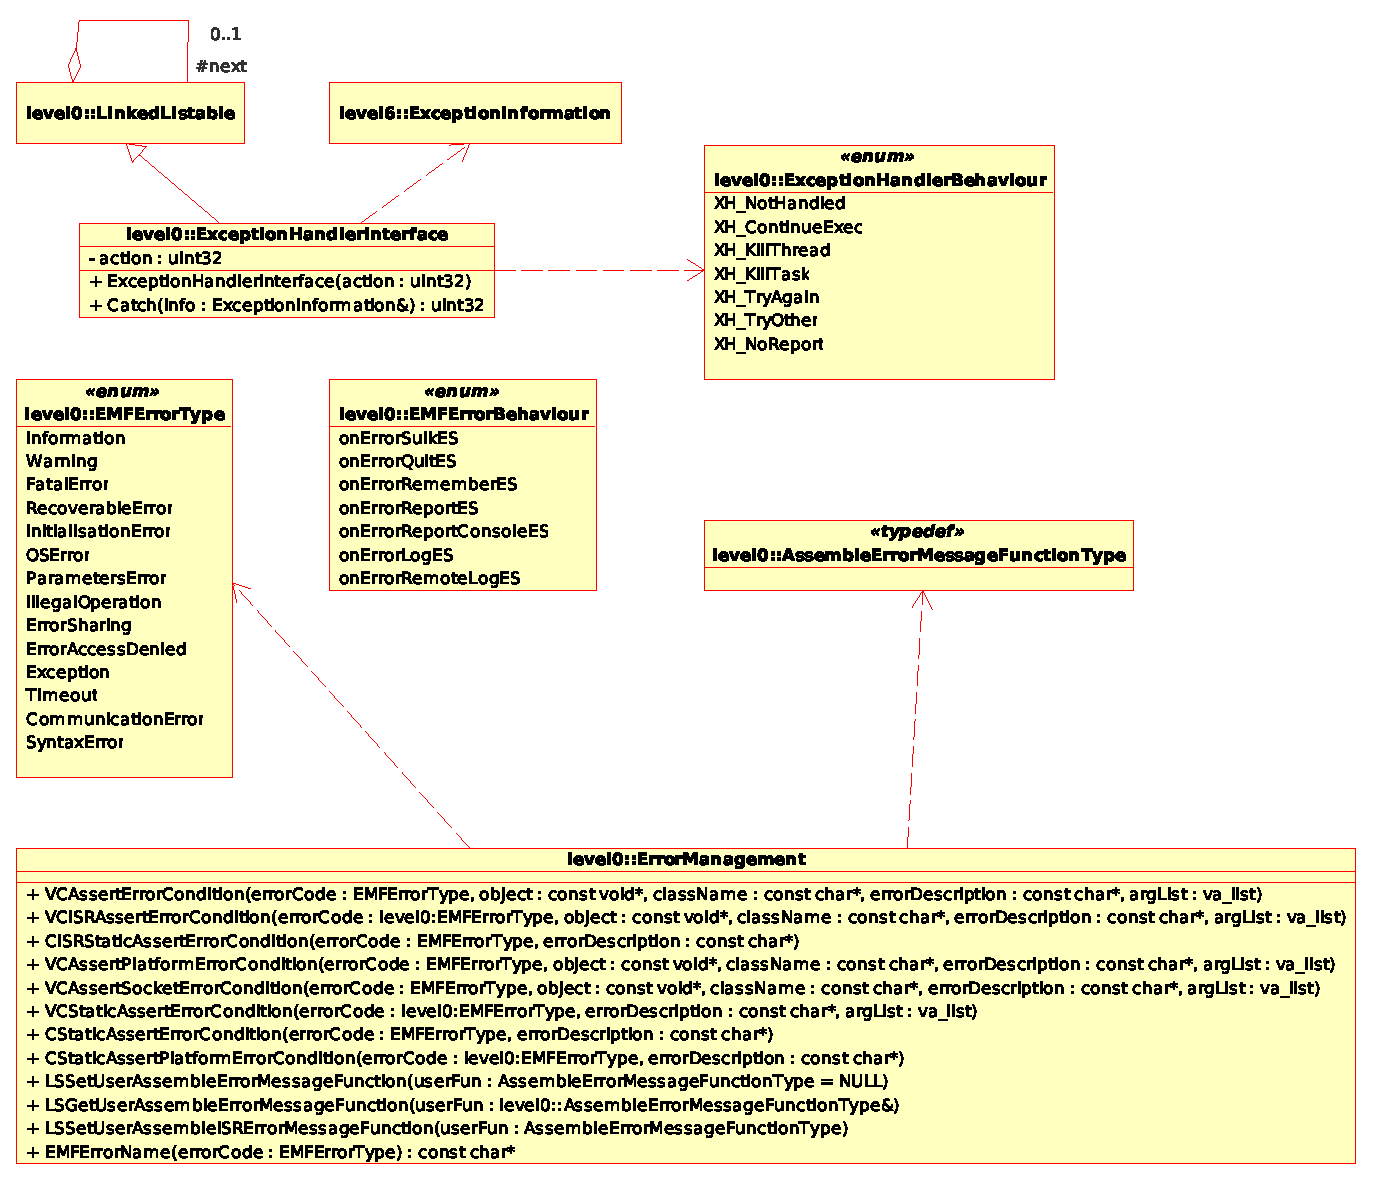
\includegraphics[width=0.93\textwidth]{level0/level0-err.eps}
  \caption{BaseLib Level0 errors and exceptions classes}
  \label{f:level0:err}
 \end{center}
\end{figure}

There are a great number of \texttt{enum}: \texttt{EMFErrorType} (in \textit{level0/ErrorManagement.h}), \texttt{EMFErrorBehaviour} (in \textit{level0/ErrorManagement.h})and \texttt{ExceptionHandlerBehaviour} (in \textit{level0/ExceptionHandlerDefinition.h}).



\subsubsection{ErrorManagement}
\texttt{[ErrorMamagemet.h, ErrorMamagemet.cpp]}\\
File \textit{level0/ErrorManagement.h} basically is a soup of C functions that print out formatted strings on some stream like for example the standard output or on a remote logger. Each function can be used in a precise scenario. Then follow a brief discussion about them.\\


Function \texttt{VCAssertErrorCondition} sets the error status and depending on setup does appropriate action; this call is to be called from static members. Function \texttt{VCISRAssertErrorCondition} like the previous one sets the error status and depending on setup does appropriate action, this call is to be called from Interrupt Service Routines. Function \texttt{CISRStaticAssertErrorCondition} sets the error status and depending on setup does appropriate action, also such call is to be called from Interrupt Service Routines (it is the same as the previous one except for the number of arguments, in such last function you have a variable argument list.\\ 

\texttt{VCAssertPlatformErrorCondition} sets the error status to \textit{platform error} and depending on setup does appropriate action, \texttt{VCAssertSocketErrorCondition} sets the error status to \textit{socket error} and depending on setup does appropriate action.\\

The function \texttt{VCStaticAssertErrorCondition} sets the error status and depending on setup does appropriate action, this call is to be called from static members; function \texttt{CStaticAssertErrorCondition} sets the error status and depending on setup does appropriate action, this call is to be called from static members. \texttt{CStaticAssertPlatformErrorCondition} sets the error status and depending on setup does appropriate action.

\begin{lstlisting}[
extendedchars=true,%
basicstyle=\fontfamily{pcr}\fontseries{m}\selectfont\footnotesize, %
stepnumber=1,%
numberstyle=\tiny,%
keywordstyle=\footnotesize\tt ,%
language=C++]
   void VCAssertErrorCondition(EMFErrorType errorCode,const void* object,
      const char* className,const char* errorDescription,va_list argList);
   void VCISRAssertErrorCondition(EMFErrorType errorCode,const void* object,
      const char* className,const char* errorDescription,va_list argList);
   void CISRStaticAssertErrorCondition(EMFErrorType errorCode,
      const char *errorDescription,...);

   void VCAssertPlatformErrorCondition(EMFErrorType errorCode,const void* object,
      const char* className,const char* errorDescription,va_list argList);
   void VCAssertSocketErrorCondition(EMFErrorType errorCode,const void* object,
      const char* className,const char* errorDescription,va_list argList);

   void VCStaticAssertErrorCondition(EMFErrorType errorCode,
      const char* errorDescription,va_list argList);
   void CStaticAssertErrorCondition(EMFErrorType errorCode,
      const char* errorDescription,...);
   void CStaticAssertPlatformErrorCondition(EMFErrorType errorCode,
      const char* errorDescription,...);
\end{lstlisting}

Function \texttt{LSSetUserAssembleErrorMessageFunction} sets the handler for error messages, function \texttt{LSGetUserAssembleErrorMessageFunction} gets a reference to the handler for error messages, \texttt{LSSetUserAssembleISRErrorMessageFunction} sets the handler for error messages coming from interrupts. Finally the function \texttt{EMFErrorName} translate an error encoded in \texttt{EMFErrorType} to an error name in C string format (\texttt{NULL}) terminated char array).

\begin{lstlisting}[
extendedchars=true,%
basicstyle=\fontfamily{pcr}\fontseries{m}\selectfont\footnotesize, %
stepnumber=1,%
numberstyle=\tiny,%
keywordstyle=\footnotesize\tt ,%
language=C++]
   void LSSetUserAssembleErrorMessageFunction(AssembleErrorMessageFunctionType userFun=NULL);
   void LSGetUserAssembleErrorMessageFunction(AssembleErrorMessageFunctionType &userFun);
   void LSSetUserAssembleISRErrorMessageFunction(AssembleErrorMessageFunctionType userFun);

   const char *EMFErrorName(EMFErrorType errorCode);
\end{lstlisting}



\subsubsection{ExceptionHandlerInterface}
\texttt{[ExceptionHandlerInterface.h]}\\
Class \texttt{ExceptionHandlerInterface} is an exception handler plugin interface. Is not a real C++ interface. There is only one abstract attribute \texttt{action} that defines what to do in case of exception. The constructor let you set the default handling in case of an exception. The method \texttt{Catch} return the action to be performed in case of an exception.

\begin{lstlisting}[
extendedchars=true,%
basicstyle=\fontfamily{pcr}\fontseries{m}\selectfont\footnotesize, %
stepnumber=1,%
numberstyle=\tiny,%
keywordstyle=\footnotesize\tt ,%
language=C++]
private:
   uint32 action;
public:
   ExceptionHandlerInterface(uint32 action=XH_NotHandled);
   virtual uint32 Catch(ExceptionInformation& info);
\end{lstlisting}



\subsection{Design Notes}
Take a look to Figure \ref{f:level0:err} is not a good design choice to have a dependency from level0 to level6: the code must be reorganized. The exception handling pluggable interface is a really nice idea.



\section{Memory}

This section group together classes depicted in Figure \ref{f:level0:mem}. Those classes have no strong link between them but are all about memory: shared memory handling, at OS level, is done by \texttt{SharedMemory} class, basic string management via \texttt{BString}; endianity support is handle via \texttt{Endianity} and memory basic type conversion is possible using \texttt{Intel16}, \texttt{IntelU16}, \texttt{Intel32},\texttt{IntelU32} classes. Such classes have to be extended also to \texttt{Intel64} and \texttt{IntelU64} as well.

\begin{figure}[h!]
 \begin{center}
  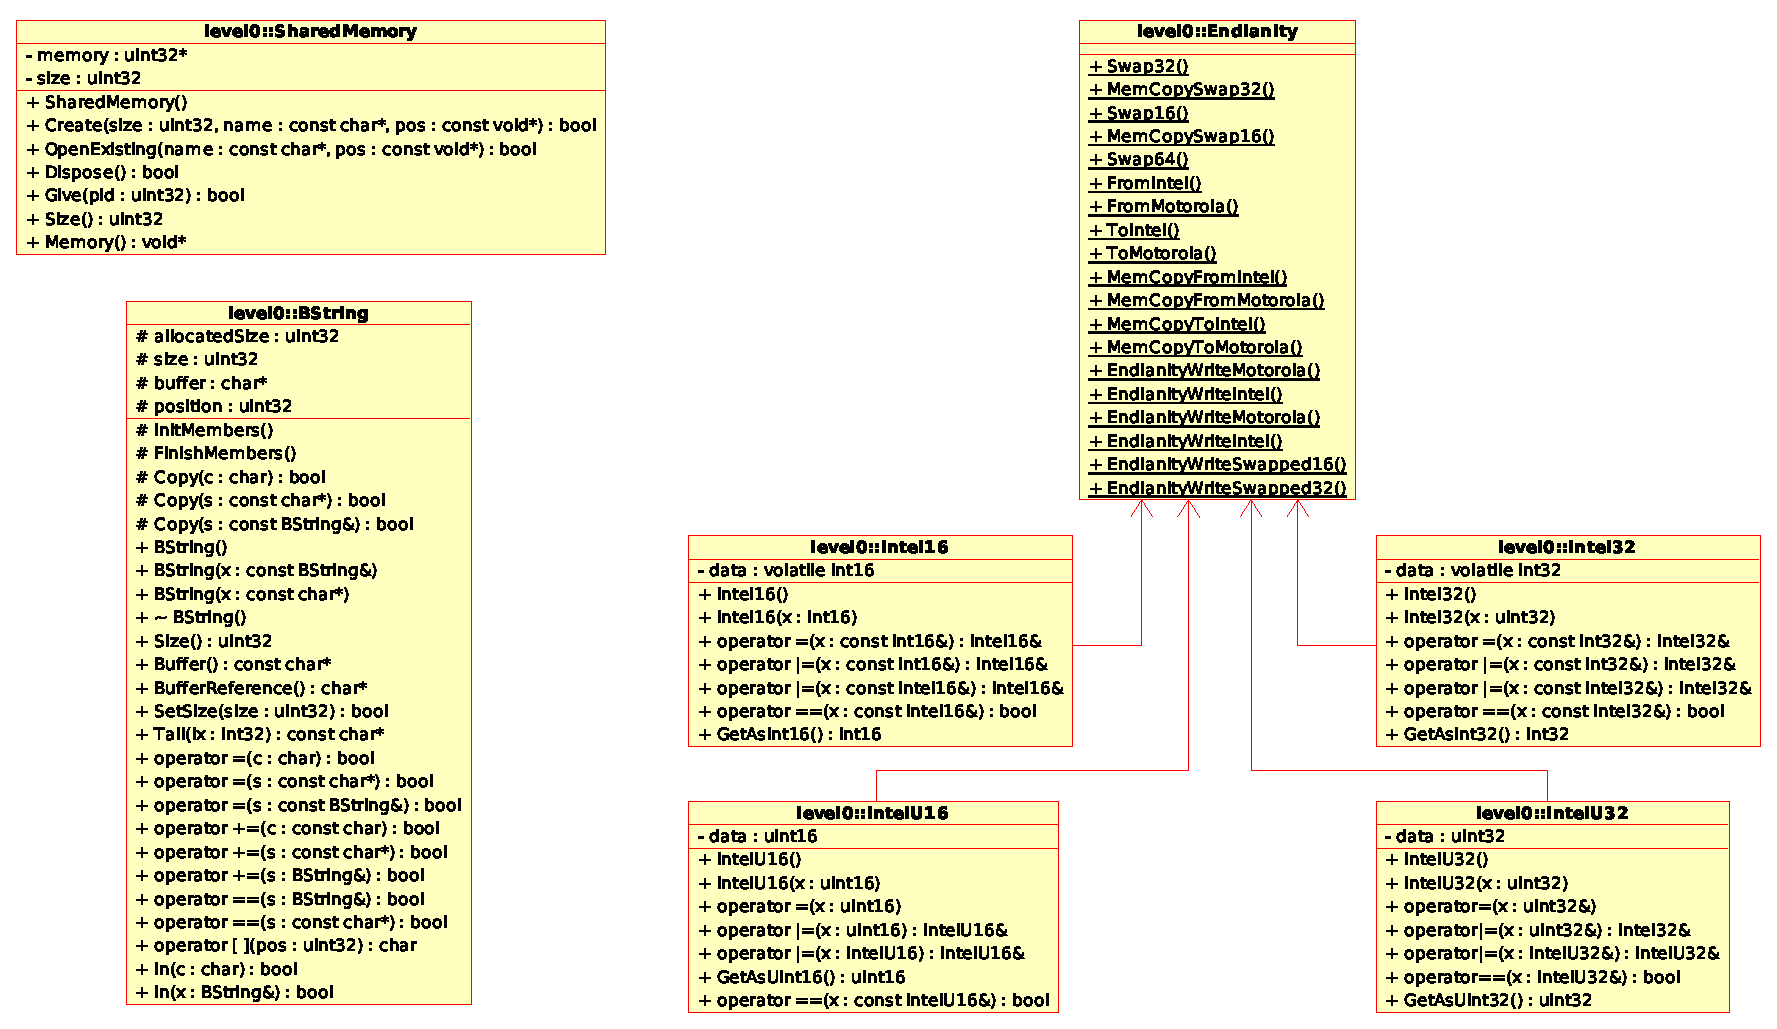
\includegraphics[width=\textwidth]{level0/level0-mem.eps}
  \caption{BaseLib Level0 memory classes}
  \label{f:level0:mem}
 \end{center}
\end{figure}

Some of those classes can be moved to a different category due to the implementation and logical dependency, for example class \texttt{SharedMemory} is thightly bounded to the OS so can be moved to \textit{arch} subdirectory, the same can be done for the class \texttt{Endianity} but that class has many dependecies in this section. Class \texttt{BString} can be moved to \textit{streams} subdirectory.



\subsubsection{SharedMemory}
\texttt{[SharedMemory.h, SharedMemory.cpp]}\\
This class is the most relevant in this group: it provides function to access shared memory. It holds attributes to the current shared memory address and to the current shared memory size (\texttt{memory}, \texttt{size}). There are others attributes with a strong dependence on the OS and OS's library, i.e. in Linux the class is implemented using SystemV Shared Memory.

\begin{lstlisting}[
extendedchars=true,%
basicstyle=\fontfamily{pcr}\fontseries{m}\selectfont\footnotesize, %
stepnumber=1,%
numberstyle=\tiny,%
keywordstyle=\footnotesize\tt ,%
language=C++]
private:
   uint32* memory;
   uint32 size;

#if (defined (_WIN32) || defined(_RSXNT))
   HANDLE handle;
#elif defined(_RTAI)
   unsigned long number;
#elif defined(_LINUX)
   key_t key;
   int id;
#endif
\end{lstlisting}

The constructor require no arguments and simply initialize the attributes in the class. \texttt{Size} simply return the size of the shared memory and \texttt{Memory} the start address of the shared memory, no check is done to test if the shared memory was just created or not, i.e. if the shared memory was not created jet the class must return an error.\\


The method \texttt{Create} create a new shared memory buffer by name \texttt{name} (in OS/2 the \texttt{pos} is disregarded); \texttt{OpenExisting} is used to open an existing share memory in the system by name.
Last two functions are from OS/2 operating system and are not fully ported to other operating systems. \texttt{Dispose} dispose the use of the shared memory and \texttt{Give} release the use of the shared memory. If \texttt{Create} is used to create a shared memory then \texttt{Dispose} is used to return the shared memory to the system. Pay attention that no destructor is coded so is not safe to not return the memory to the system. Difference between \texttt{Give} and \texttt{Dispose} is not really clear.

\begin{lstlisting}[
extendedchars=true,%
basicstyle=\fontfamily{pcr}\fontseries{m}\selectfont\footnotesize, %
stepnumber=1,%
numberstyle=\tiny,%
keywordstyle=\footnotesize\tt ,%
language=C++]
public:
   SharedMemory();
   uint32 Size();
   void* Memory();

   bool Create(uint32 size,const char* name,const void* pos=0);
   bool OpenExisting(const char* name,const void* pos=0);
   bool Dispose(void)
   bool Give(uint32 pid);
\end{lstlisting}



\subsubsection{BString}
\texttt{[BString.h, BString.cpp]}\\
The class \texttt{BString} is the basic implementation of a string, the class want let user treat a string like a file; reading and writing are done on a specific position.\\


Starting with the attributes, the first attribute, \texttt{allocatedSize}, is the size of the allocated memory block for the string; \texttt{size} represent the size of the used memory block minus one (it excludes the 0 char); \texttt{buffer} holds the memory buffer address and \texttt{position} is the currently seek position.\\


Other protected methods are: \texttt{InitMembers} and \texttt{FinishMembers} used for constructor and deconstructor.
Copy methods (\texttt{Copy}) let the user copy a character, a string and a \texttt{BString} into the \texttt{BString} buffer.

\begin{lstlisting}[
extendedchars=true,%
basicstyle=\fontfamily{pcr}\fontseries{m}\selectfont\footnotesize, %
stepnumber=1,%
numberstyle=\tiny,%
keywordstyle=\footnotesize\tt ,%
language=C++]
protected:
   uint32 allocatedSize;
   uint32 size;
   char* buffer;
   uint32 position;

   void InitMembers();
   void FinishMembers();

   bool Copy(char* c);
   bool Copy(const char* s);
   bool Copy(const BString& s);
\end{lstlisting}

The first constructor creates an empty string; second constructor is the copy constructor and the last constructor build up a \texttt{BString} starting from a C string. Then cames the destructor.

The method \texttt{Size} return the size of the string (\texttt{size} attribute); \texttt{SetSize} clips the string size to a specified point (\texttt{size} is expressed from the start of the string). \texttt{Buffer} returns a read only access to the internal buffer, \texttt{BufferReference} returns a read/write access to the internal buffer and \texttt{Tail} returns a read only pointer to the tail of the buffer.

Methods \texttt{In} checks if a char is in the string.

\begin{lstlisting}[
extendedchars=true,%
basicstyle=\fontfamily{pcr}\fontseries{m}\selectfont\footnotesize, %
stepnumber=1,%
numberstyle=\tiny,%
keywordstyle=\footnotesize\tt ,%
language=C++]
public:
   inline BString();
   inline BString(const BString& x);
   inline BString(const char* x);
   virtual ~BString();

   inline uint32 Size() const;
   inline bool SetSize(uint32 size);

   inline const char* Buffer() const;
   inline char* BufferReference() const;
   inline const char* Tail(int32 ix ) const;

   inline bool In(char c) const;
   inline bool In(BString& x) const;
\end{lstlisting}

The following operators redefinition eases the work with strings. First three \texttt{operator=} lets sets a \texttt{BString} to be a copy of the input parameter; methods \texttt{operator+=} address the concatenation between a \texttt{BString} and a single char, a C string and a \texttt{BString} object; redefinition of \texttt{opertator==} lets compare differents string objects. \texttt{operator[]} allows access to character within the buffer, argument \texttt{pos} is the position in the buffer to be accessed.

\begin{lstlisting}[
extendedchars=true,%
basicstyle=\fontfamily{pcr}\fontseries{m}\selectfont\footnotesize, %
stepnumber=1,%
numberstyle=\tiny,%
keywordstyle=\footnotesize\tt ,%
language=C++]
   inline bool operator=(char c);
   inline bool operator=(const char *s);
   inline bool operator=(const BString &s);
   inline bool operator+=(const char c);
   inline bool operator+=(const char *s);
   inline bool operator+=(BString &s);
   inline bool operator==(BString &s) const;
   inline bool operator==(const char *s) const;
   inline char operator[](uint32 pos);
\end{lstlisting}



\subsubsection{Endianity}
\texttt{[Endianity.h]}\\
The endianity class implements endianity conversion between types. Basically many methods were cut in Figure \ref{f:level0:mem} to fit the UML schema in the page. We now explore the methods it offers.

Core methods are first coded and basically do all the work. The first \texttt{Swap32} method swaps the 4 bytes in a 32 bit number, i.e. simply changes the endianity; the second \texttt{Swap32} swaps 4 bytes in a 32bit vector; \texttt{MemCopySwap32} swaps the 4 bytes while copying a vector of 32 bit numbers.

The first \texttt{Swap16} method swaps the 2 bytes in a 16 bit number, i.e. changes the endianity; the second \texttt{Swap16} swaps 2 bytes in a 16bit vector; \texttt{MemCopySwap16} swaps the 2 bytes while copying a vector of 16 bit numbers.

Last \texttt{Swap64} method swaps the 8 bytes in a 64 bit number.

\begin{lstlisting}[
extendedchars=true,%
basicstyle=\fontfamily{pcr}\fontseries{m}\selectfont\footnotesize, %
stepnumber=1,%
numberstyle=\tiny,%
keywordstyle=\footnotesize\tt ,%
language=C++]
public:
   static inline void Swap32(volatile void *x);
   static inline void Swap32(volatile void *x,uint32 sizer);
   static inline void MemCopySwap32(volatile void *dest,volatile const void *src,uint32 sizer);

   static inline void Swap16(volatile void *x);
   static inline void Swap16(volatile void *x,uint32 sizer);
   static inline void MemCopySwap16(volatile void *dest,volatile const void *src,uint32 sizer);

   static inline void Swap64(volatile void *x);
\end{lstlisting}

The following function has a different implementation if compiled on different architecture (infact this class will be moved in \textit{arch}). The first overloaded method \texttt{FromMotorola} need in input a number in \textit{Motorola} format (i.e. big endian) and convert it in the currently system endianity format. \texttt{FromIntel} need in input a number in \textit{Intel} format (i.e. little endian) and convert it in the currently system endianity format. \texttt{ToMotorola} covert the value in big endian and \texttt{ToIntel} convert the value in little endian.

All such methods use the before presented methods.

\begin{lstlisting}[
extendedchars=true,%
basicstyle=\fontfamily{pcr}\fontseries{m}\selectfont\footnotesize, %
stepnumber=1,%
numberstyle=\tiny,%
keywordstyle=\footnotesize\tt ,%
language=C++]
   static inline void FromMotorola(volatile double &x);
   static inline void FromMotorola(volatile float &x);
   static inline void FromMotorola(volatile uint64 &x);
   static inline void FromMotorola(volatile uint32 &x);
   static inline void FromMotorola(volatile uint16 &x);
   static inline void FromMotorola(volatile int64 &x);
   static inline void FromMotorola(volatile int32 &x);
   static inline void FromMotorola(volatile int16 &x);

   static inline void FromIntel(volatile double &x);
   static inline void FromIntel(volatile float &x);
   static inline void FromIntel(volatile uint64 &x);
   static inline void FromIntel(volatile uint32 &x);
   static inline void FromIntel(volatile uint16 &x);
   static inline void FromIntel(volatile int64 &x);
   static inline void FromIntel(volatile int32 &x);
   static inline void FromIntel(volatile int16 &x);

   static inline void ToMotorola(volatile double &x);
   static inline void ToMotorola(volatile float &x);
   static inline void ToMotorola(volatile uint64 &x);
   static inline void ToMotorola(volatile uint32 &x);
   static inline void ToMotorola(volatile uint16 &x);
   static inline void ToMotorola(volatile int64 &x);
   static inline void ToMotorola(volatile int32 &x);
   static inline void ToMotorola(volatile int16 &x);

   static inline void ToIntel(volatile double &x);
   static inline void ToIntel(volatile float &x);
   static inline void ToIntel(volatile uint64 &x);
   static inline void ToIntel(volatile uint32 &x);
   static inline void ToIntel(volatile uint16 &x);
   static inline void ToIntel(volatile int64 &x);
   static inline void ToIntel(volatile int32 &x);
   static inline void ToIntel(volatile int16 &x);
\end{lstlisting}

The group of methods that comes are really equivalent to the ones above but instead of swapping a single value they swap an entire vector of values. The signature of methods is fully reported here.

\begin{lstlisting}[
extendedchars=true,%
basicstyle=\fontfamily{pcr}\fontseries{m}\selectfont\footnotesize, %
stepnumber=1,%
numberstyle=\tiny,%
keywordstyle=\footnotesize\tt ,%
language=C++]
   static inline void MemCopyFromMotorola(float *dest,const float *src,uint32 size);
   static inline void MemCopyFromMotorola(uint32 *dest,const uint32 *src,uint32 size);
   static inline void MemCopyFromMotorola(uint16 *dest,const uint16 *src,uint32 size);
   static inline void MemCopyFromMotorola(int32 *dest,const int32 *src,uint32 size);
   static inline void MemCopyFromMotorola(int16 *dest,const int16 *src,uint32 size);

   static inline void MemCopyFromIntel(float *dest,const float *src,uint32 size);
   static inline void MemCopyFromIntel(uint32 *dest,const uint32 *src,uint32 size);
   static inline void MemCopyFromIntel(uint16 *dest,const uint16 *src,uint32 size);
   static inline void MemCopyFromIntel(int32 *dest,const int32 *src,uint32 size);
   static inline void MemCopyFromIntel(int16 *dest,const int16 *src,uint32 size);

   static inline void MemCopyToMotorola(float *dest,const float *src,uint32 size);
   static inline void MemCopyToMotorola(uint32 *dest,const uint32 *src,uint32 size);
   static inline void MemCopyToMotorola(uint16 *dest,const uint16 *src,uint32 size);
   static inline void MemCopyToMotorola(int32 *dest,const int32 *src,uint32 size);
   static inline void MemCopyToMotorola(int16 *dest,const int16 *src,uint32 size);

   static inline void MemCopyToIntel(float *dest,const float *src,uint32 size);
   static inline void MemCopyToIntel(uint32 *dest,const uint32 *src,uint32 size);
   static inline void MemCopyToIntel(uint16 *dest,const uint16 *src,uint32 size);
   static inline void MemCopyToIntel(int32 *dest,const int32 *src,uint32 size);
   static inline void MemCopyToIntel(int16 *dest,const int16 *src,uint32 size);
\end{lstlisting}

Last methods, that are to be moved to streams, all use the \texttt{fwrite} function (binary stream output) but does the same things as the one above.

\begin{lstlisting}[
extendedchars=true,%
basicstyle=\fontfamily{pcr}\fontseries{m}\selectfont\footnotesize, %
stepnumber=1,%
numberstyle=\tiny,%
keywordstyle=\footnotesize\tt ,%
language=C++]
   static inline void EndianityWriteMotorola(int8 &x,FILE *f);
   static inline void EndianityWriteMotorola(int16 &x,FILE *f);
   static inline void EndianityWriteMotorola(int32 &x,FILE *f);
   static inline void EndianityWriteMotorola(uint8 &x,FILE *f);
   static inline void EndianityWriteMotorola(uint16 &x,FILE *f);
   static inline void EndianityWriteMotorola(uint32 &x,FILE *f);

   static inline void EndianityWriteIntel(int8 &x,FILE *f);
   static inline void EndianityWriteIntel(int16 &x,FILE *f);
   static inline void EndianityWriteIntel(int32 &x,FILE *f);
   static inline void EndianityWriteIntel(uint8 &x,FILE *f);
   static inline void EndianityWriteIntel(uint16 &x,FILE *f);
   static inline void EndianityWriteIntel(uint32 &x,FILE *f);

   static inline void EndianityWriteMotorola(int8 *x,uint32 n,FILE *f);
   static inline void EndianityWriteMotorola(int16 *x,uint32 n,FILE *f);
   static inline void EndianityWriteMotorola(int32 *x,uint32 n,FILE *f);
   static inline void EndianityWriteMotorola(uint8 *x,uint32 n,FILE *f);
   static inline void EndianityWriteMotorola(uint16 *x,uint32 n,FILE *f);
   static inline void EndianityWriteMotorola(uint32 *x,uint32 n,FILE *f);

   static inline void EndianityWriteIntel(int8 *x,uint32 n,FILE *f);
   static inline void EndianityWriteIntel(int16 *x,uint32 n,FILE *f);
   static inline void EndianityWriteIntel(int32 *x,uint32 n,FILE *f);
   static inline void EndianityWriteIntel(uint8 *x,uint32 n,FILE *f);
   static inline void EndianityWriteIntel(uint16 *x,uint32 n,FILE *f);
   static inline void EndianityWriteIntel(uint32 *x,uint32 n,FILE *f);

   static void EndianityWriteSwapped16(void *x,uint32 n,FILE *f);
   static void EndianityWriteSwapped32(void *x,uint32 n,FILE *f);
\end{lstlisting}



\subsubsection{Intel16, IntelU16, Intel32, IntelU32}
\texttt{[Intel16.h, IntelU16.h, Intel32.h, IntelU32.h]}\\
Those classes implements a 16 bit integer in little endian encoding, a 16 bit unsigned int in little endian encoding, a 32 bit integer in little endian encoding and a 32 bit unsigned integer in little endian encoding.

Basically they all have the same interface with the same methods, constructors and operators ridefinition. We just cut and past the class definition of \texttt{Intel16}.

\begin{lstlisting}[
extendedchars=true,%
basicstyle=\fontfamily{pcr}\fontseries{m}\selectfont\footnotesize, %
stepnumber=1,%
numberstyle=\tiny,%
keywordstyle=\footnotesize\tt ,%
language=C++]
class Intel16 {
private:
   volatile int16 data;
public:
   inline Intel16();
   inline Intel16(int16 x);

   inline Intel16& operator= (const int16& x);
   inline Intel16& operator|= (const int16& x);
   inline Intel16& operator|= (const Intel16& x);
   inline bool operator == (const Intel16& x);

   inline int16 GetAsInt16();
};
\end{lstlisting}



\subsection{Design Notes}
This section doesn't need to much notes because classes are probably not well grouped together. Some class can be moved to another groups.
It is really important that the \texttt{SharedMemory} class has a distructor that will destroy the give back the shared memory helded to keep resource consumption under control.



\section{Processes, Threads}

\begin{figure}[h!]
 \begin{center}
  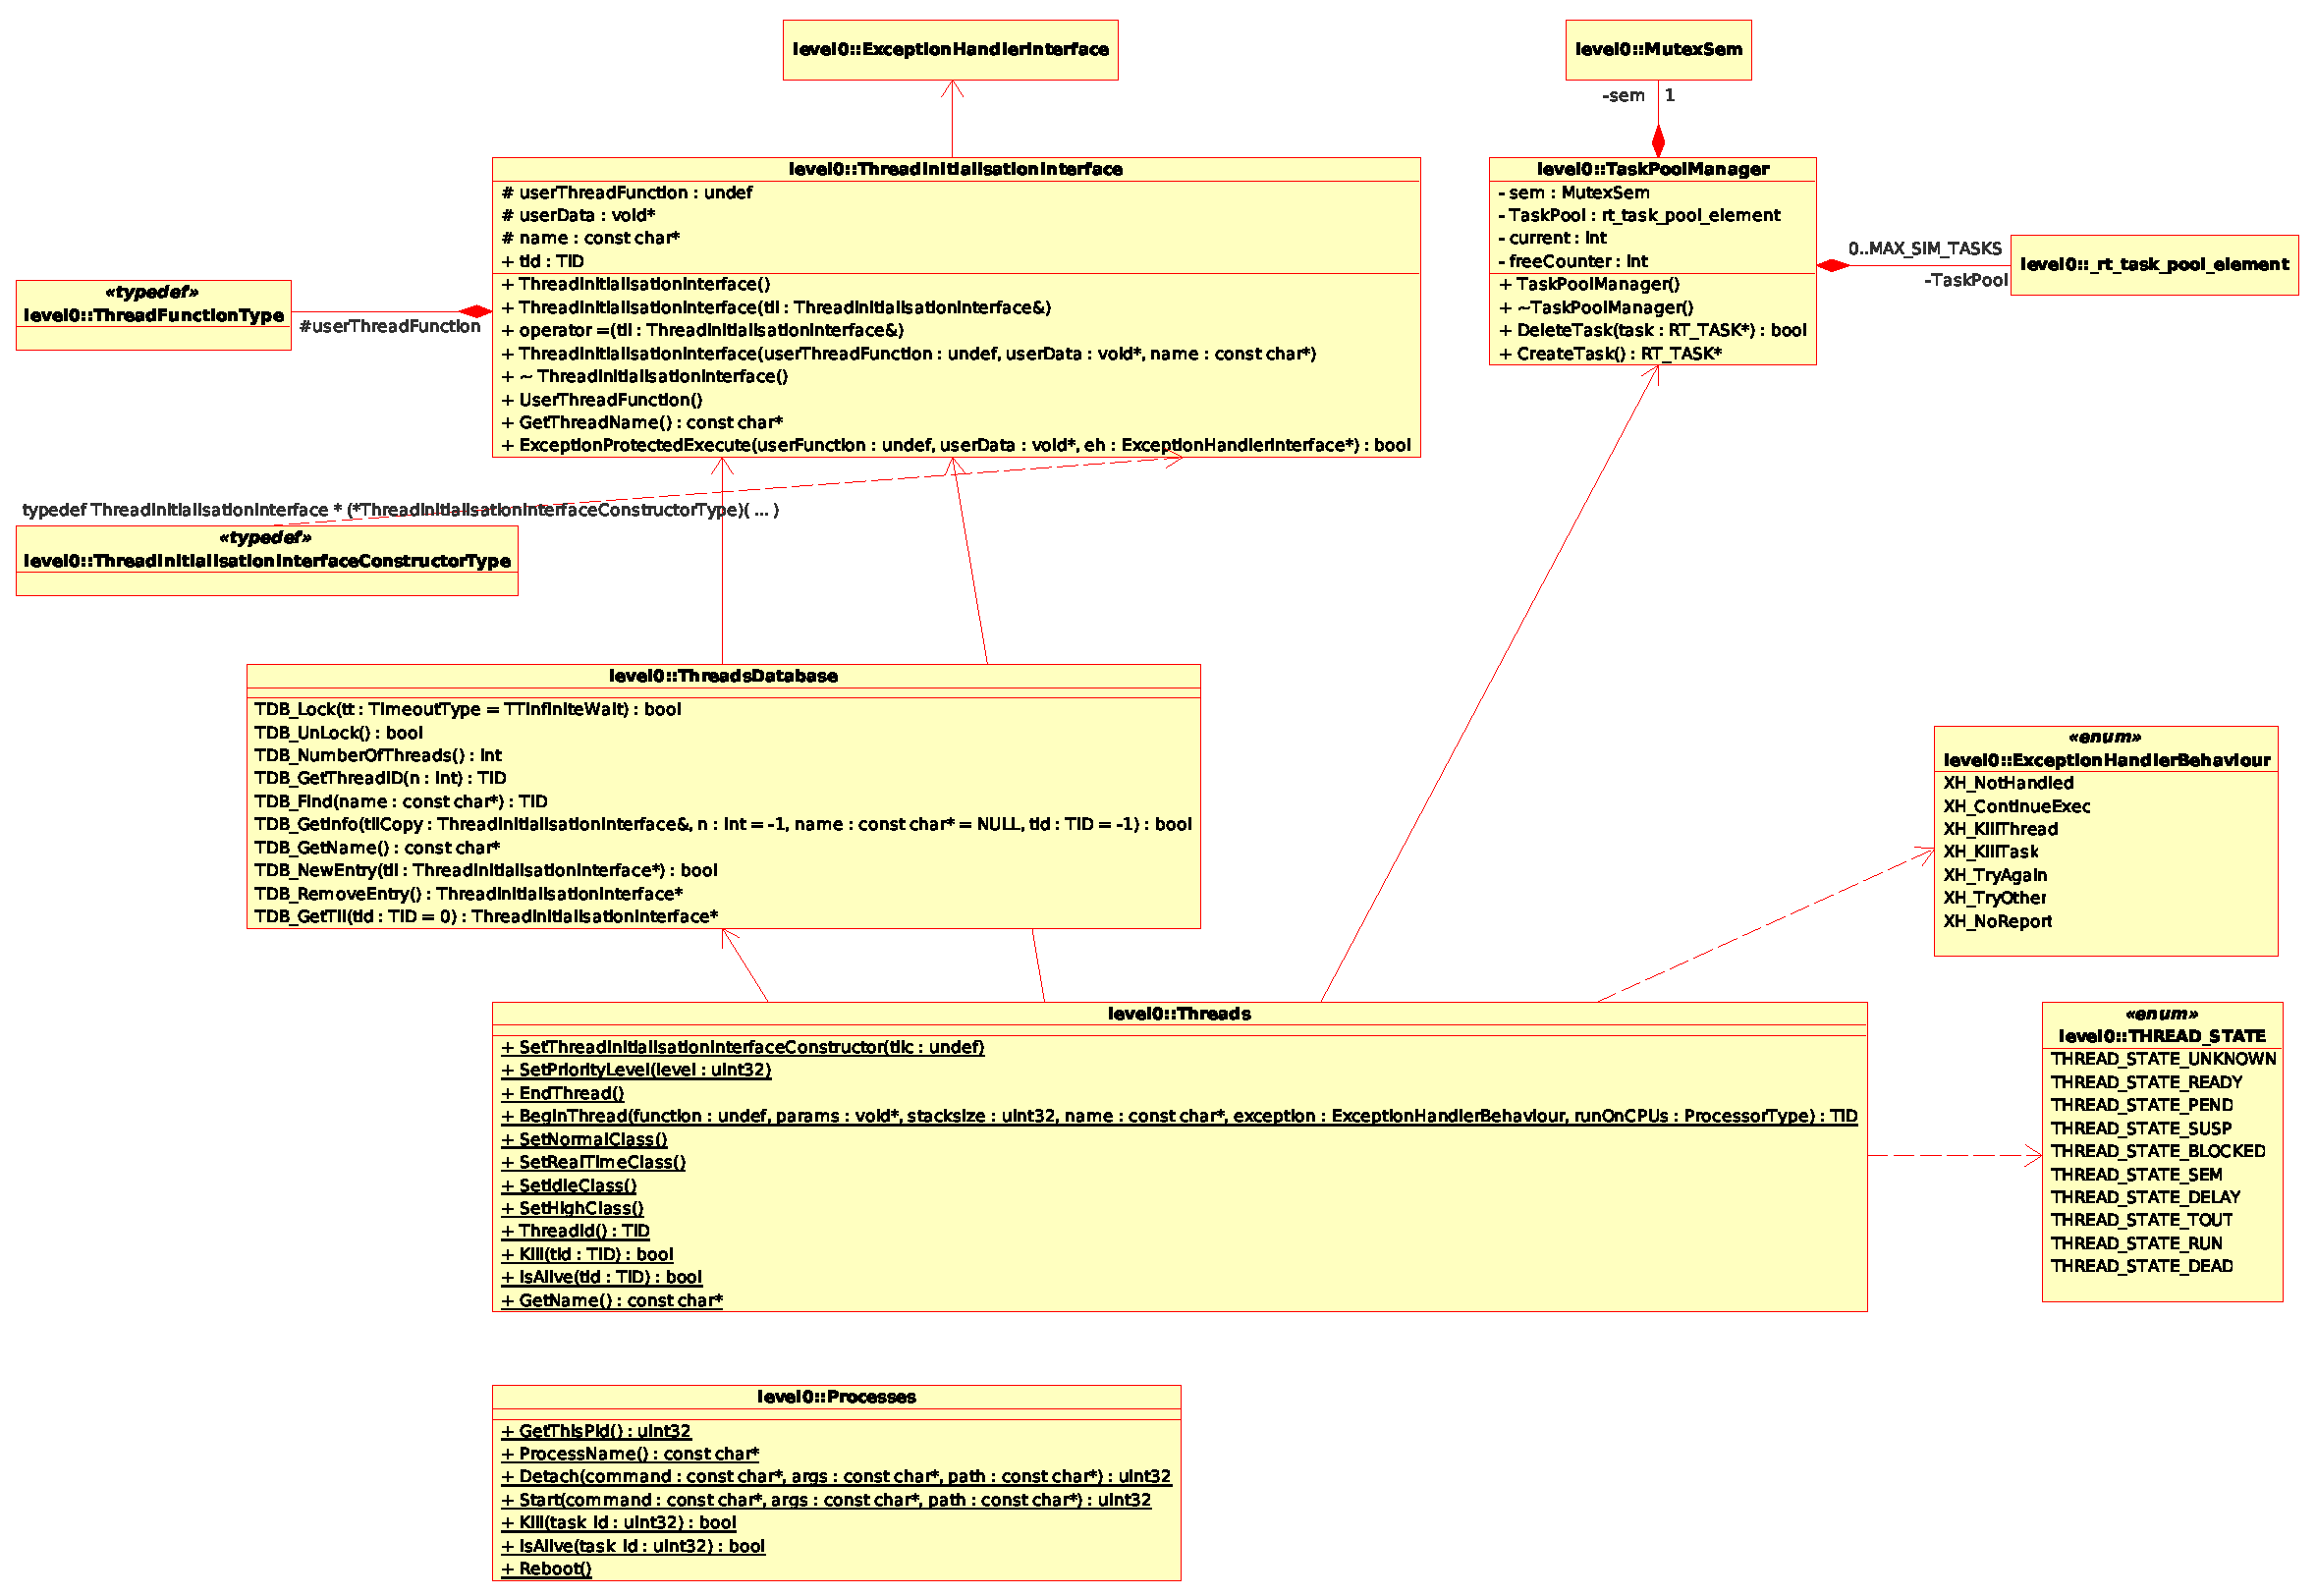
\includegraphics[width=\textwidth]{level0/level0-proc.eps}
  \caption{BaseLib Level0 proc classes}
  \label{f:level0:proc}
 \end{center}
\end{figure}

\subsubsection{ThreadInitialisationInterface}
\texttt{[ThreadInitialisationInterface.h]}\\
This class stores information associated with a specific thread. Such class is an interface used to implement a common thread initialisation procedure; despite the name \texttt{ThreadInitialisationInterface} it also provides a minimal set of functionalities; for this reason it has not been made pure virtual and can be istantiated. Let's take a look at its attributes and methods.\\

The type of a function that can be used for a thread is typedefined in \textit{level0/ThreadInitialistionInterface.h}
\begin{lstlisting}[
extendedchars=true,%
basicstyle=\fontfamily{pcr}\fontseries{m}\selectfont\footnotesize, %
stepnumber=1,%
numberstyle=\tiny,%
keywordstyle=\footnotesize\tt ,%
language=C++]
typedef void (*ThreadFunctionType)(void *parameters);
\end{lstlisting}
The attribute \texttt{userThreadFunction} is of type \texttt{ThreadFunctionType} and is the holder of a thread entry point. \texttt{userData} is
 a pointer to a structure containing thread data and \textit{name} is the name of the thread. Last attribute, a \texttt{public} one holds the thread number.

\begin{lstlisting}[
extendedchars=true,%
basicstyle=\fontfamily{pcr}\fontseries{m}\selectfont\footnotesize, %
stepnumber=1,%
numberstyle=\tiny,%
keywordstyle=\footnotesize\tt ,%
language=C++]
protected:
   ThreadFunctionType userThreadFunction;
   void* userData;
   const char* name;
public:
   TID tid;
\end{lstlisting}

There is an \texttt{operation=} ridefinition and a copy constructor; other two constructors create a new \texttt{NULL} object and a new object with a new \texttt{ThreadFunctionType}, a \texttt{userData} and a \texttt{name}.

The method \texttt{UserThreadFunction} execute the registered thread; \texttt{GetThreadName} gets the name of the thread and \texttt{ExceptionProtectedExecute} allows to call a subroutine within an exception handler protection, this implementation is a dummy one, so it must be recoded at higher levels (i.e. to be subclassed).

\begin{lstlisting}[
extendedchars=true,%
basicstyle=\fontfamily{pcr}\fontseries{m}\selectfont\footnotesize, %
stepnumber=1,%
numberstyle=\tiny,%
keywordstyle=\footnotesize\tt ,%
language=C++]
   void operator=(ThreadInitialisationInterface &tii);
   ThreadInitialisationInterface(ThreadInitialisationInterface& tii);

   ThreadInitialisationInterface();
   ThreadInitialisationInterface(ThreadFunctionType userThreadFunction,
      void* userData, const char* name);
   virtual ~ThreadInitialisationInterface();

   virtual void UserThreadFunction();
   virtual const char *GetThreadName();
   bool ExceptionProtectedExecute(ThreadFunctionType userFunction,
      void *userData, ExceptionHandlerInterface *eh);
\end{lstlisting}



\subsubsection{Threads DataBase}
\texttt{[ThreadsDatabase.h,ThreadsDatabase.cpp]}\\
The \textit{Threads DataBase} is not a class but a set of function. It is depicted in Figure \ref{f:level0:proc} only for dependency purpouse. Such entity is a register of all the threads currently running (or expected to be running) in the system. All functions that lets you manage the \textit{Threads DataBase} follows, functions can be founded in \textit{level0/ThreadsDatabase.h}.\\


\textit{Threads DataBase} (TDB) is managed via the class \texttt{Threads} the following three functions are only accessible by \textit{level0/Threads.cpp} (i.e. are not exported or declared anywhere else).
The method \texttt{TDB\_NewEntry} creates new TDB entry associated to the \texttt{ThreadInitialisationInterface} object passed by pointer. Note that a \texttt{Threads} object is not a subclass of \texttt{ThreadInitialisationInterface}. The method \texttt{TDB\_RemoveEntry} destroy the TDB entry associated wtih the current calling thread, note that the method has no arguments. The method \texttt{TDB\_GetTII} access private thread information, on timeout returns \texttt{NULL}.

\begin{lstlisting}[
extendedchars=true,%
basicstyle=\fontfamily{pcr}\fontseries{m}\selectfont\footnotesize, %
stepnumber=1,%
numberstyle=\tiny,%
keywordstyle=\footnotesize\tt ,%
language=C++]
   bool TDB_NewEntry(ThreadInitialisationInterface *tii);
   ThreadInitialisationInterface* TDB_RemoveEntry();
   ThreadInitialisationInterface* TDB_GetTII(TID tid=0);
\end{lstlisting}

Now comes some generic usable functions. Every time a user want to access the TDB it must request a lock to use it with \texttt{TDB\_Lock} and unlock with \texttt{TDB\_UnLock}.

The method \texttt{TDB\_NumberOfThreads} returns the number of threads registered in the database. \texttt{TDB\_GetThreadID} retrieves the TID of thread \texttt{n}, the method \texttt{TDB\_Find} return the TID of thread named \texttt{name}.
\texttt{TDB\_GetInfo} retrieves information about a thread identified either by \texttt{name} or \texttt{TID} or index; \texttt{TDB\_GetName} retrieves pointer to name in \texttt{ThreadInitialisationInterface} attribute for current thread.

\begin{lstlisting}[
extendedchars=true,%
basicstyle=\fontfamily{pcr}\fontseries{m}\selectfont\footnotesize, %
stepnumber=1,%
numberstyle=\tiny,%
keywordstyle=\footnotesize\tt ,%
language=C++]
   bool TDB_Lock(TimeoutType tt = TTInfiniteWait);
   bool TDB_UnLock();

   int TDB_NumberOfThreads();
   TID TDB_GetThreadID(int n);
   TID TDB_Find(const char* name);
   bool TDB_GetInfo(ThreadInitialisationInterface& tiiCopy,
      int n=-1,const char* name=NULL,TID tid=(TID)-1);
   const char* TDB_GetName();
\end{lstlisting}

Differently with others \textit{DataBase}'s structures this \textit{Threads DataBase} doesn't relay on a linked list but on an array of pointers to \texttt{ThreadInitialisationInterface} objects.



\subsubsection{Threads}
\texttt{[Threads.h, Threads.cpp]}\\

This is the core threads class, it provides for thread registration in the \textit{Threads Database} and provide a complete interface to thread managment (processors mask are managed via the \texttt{ProcessorType} class).\\


The method \texttt{SetThreadInitialisationInterfaceConstructor} sets the function used to build the thread initialisation interface. An \texttt{ThreadInitialisationInterface} object is created using either the default value or the parameter passed to the function by the \texttt{BeginThread} method. The method \texttt{SetPriorityLevel} changes thread priority; applies only to current thread 0..31 (on windows it is actually /4 ). \texttt{EndThread} is called implicitly at the end of the main thread function, calling this method leaves some allocated memory unfreed. Calling \texttt{BeginThread} will start a thred this method will dynamically allocate an object of type \texttt{ThreadInitialisationInterface} using the function hook \texttt{ThreadInitialisationInterfaceConstructor}; this allows the programmer to choose which constructor has to be used in the case a \texttt{ThreadInitialisationInterface} derived class had been used.

In BaseLib that is a thread based library there are four classes of priority (from the maximum priority to the minimum priority):
\begin{itemize}
 \item RealTime
 \item High
 \item Normal
 \item Low
\end{itemize}

\texttt{Threads} class define only static methods so each static method apply to the current executed thread. You can change the thread priority using \texttt{SetRealTimeClass}, \texttt{SetHighClass}, \texttt{SetNormalClass} and \texttt{SetLowClass}.

\texttt{ThreadId} method gets the current thread id; \texttt{Kill} kills a thread asynchronously; \texttt{IsAlive} checks whether thread \texttt{tid} is still alive. The method \texttt{GetName} basically retrieve thread's name.

\begin{lstlisting}[
extendedchars=true,%
basicstyle=\fontfamily{pcr}\fontseries{m}\selectfont\footnotesize, %
stepnumber=1,%
numberstyle=\tiny,%
keywordstyle=\footnotesize\tt ,%
language=C++]
public:
   static void SetThreadInitialisationInterfaceConstructor(ThreadInitialisationInterfaceConstructorType tiic);
   static void SetPriorityLevel(uint32 level);

   static void EndThread();
   static TID BeginThread(ThreadFunctionType function,
      void* parameters = NULL,
      uint32 stacksize=THREADS_DEFAULT_STACKSIZE,
      const char* name=NULL,
      ExceptionHandlerBehaviour exceptionHandlerBehaviour=XH_NotHandled,
      ProcessorType runOnCPUs=PTDefaultCPUs);

   static void SetNormalClass();
   static void SetRealTimeClass();
   static void SetIdleClass();
   static void SetHighClass();

   static TID ThreadId();
   static bool Kill(TID tid);
   static bool IsAlive(TID tid);
   static const char *GetName();
\end{lstlisting}



\subsubsection{Processes}
\texttt{[Processes.h]}\\
The class \texttt{Processes} give an interface to operating system wide functions like creating a process, i.e. loading an executable file, process index, killing a process and reboot the system. The description of functions interface follows.\\

The method \texttt{GetThisPid} returns the current's process id and \texttt{ProcessName} retrieves the name of this applicationm, it is obtained by parsing \texttt{argv[0]} it does not work if \texttt{REAL\_MAIN} is defined.\\

Methods \texttt{Detach} and \texttt{Start} are exactly the same method for every system except OS/2. \texttt{Detach} method launchs a specified command as a newly detached process and return the task id of the new process or 0 if the process has not been created; \texttt{command} argument is a pointer to a string containing the command to execute (i.e. the application that will run); \texttt{args} argument is a pointer to a string containing the arguments of the command; \texttt{path} is a pointer to a string containing the path to the command. \\

The method \texttt{Kill} lets the user kill the process specified by the \texttt{task\_id}; \texttt{IsAlive} lets query the system to know if the process specified by argument is alive; last method: \texttt{Reboot} causes the machine to reboot.

\begin{lstlisting}[
extendedchars=true,%
basicstyle=\fontfamily{pcr}\fontseries{m}\selectfont\footnotesize, %
stepnumber=1,%
numberstyle=\tiny,%
keywordstyle=\footnotesize\tt ,%
language=C++]
public:
   static uint32 GetThisPid();
   static const char *ProcessName();
   
   static uint32 Detach(const char *command,const char *args,const char *path = NULL);
   static uint32 Start(const char *command,const char *args,const char *path=NULL);
   static bool Kill(uint32 task_id);
   static bool IsAlive(uint32 task_id);

   static void Reboot();
\end{lstlisting}



\subsection{Design Notes}

Class \texttt{Processes} is likely to be moved in directory \textit{arch}. I'm not sure about the need of a \texttt{ThreadInitializationInterface}, a \texttt{ThreadInterface} can be better.



\section{Mathematic}
In this section there are some class involving mathematical conversion and complex number handling. Classes in this seciton are here listed and depicted in Figure \ref{f:level0:math}.
\begin{itemize}
 \item Complex
 \item NordFloat
 \item FastMath
\end{itemize}

\begin{figure}[h!]
 \begin{center}
  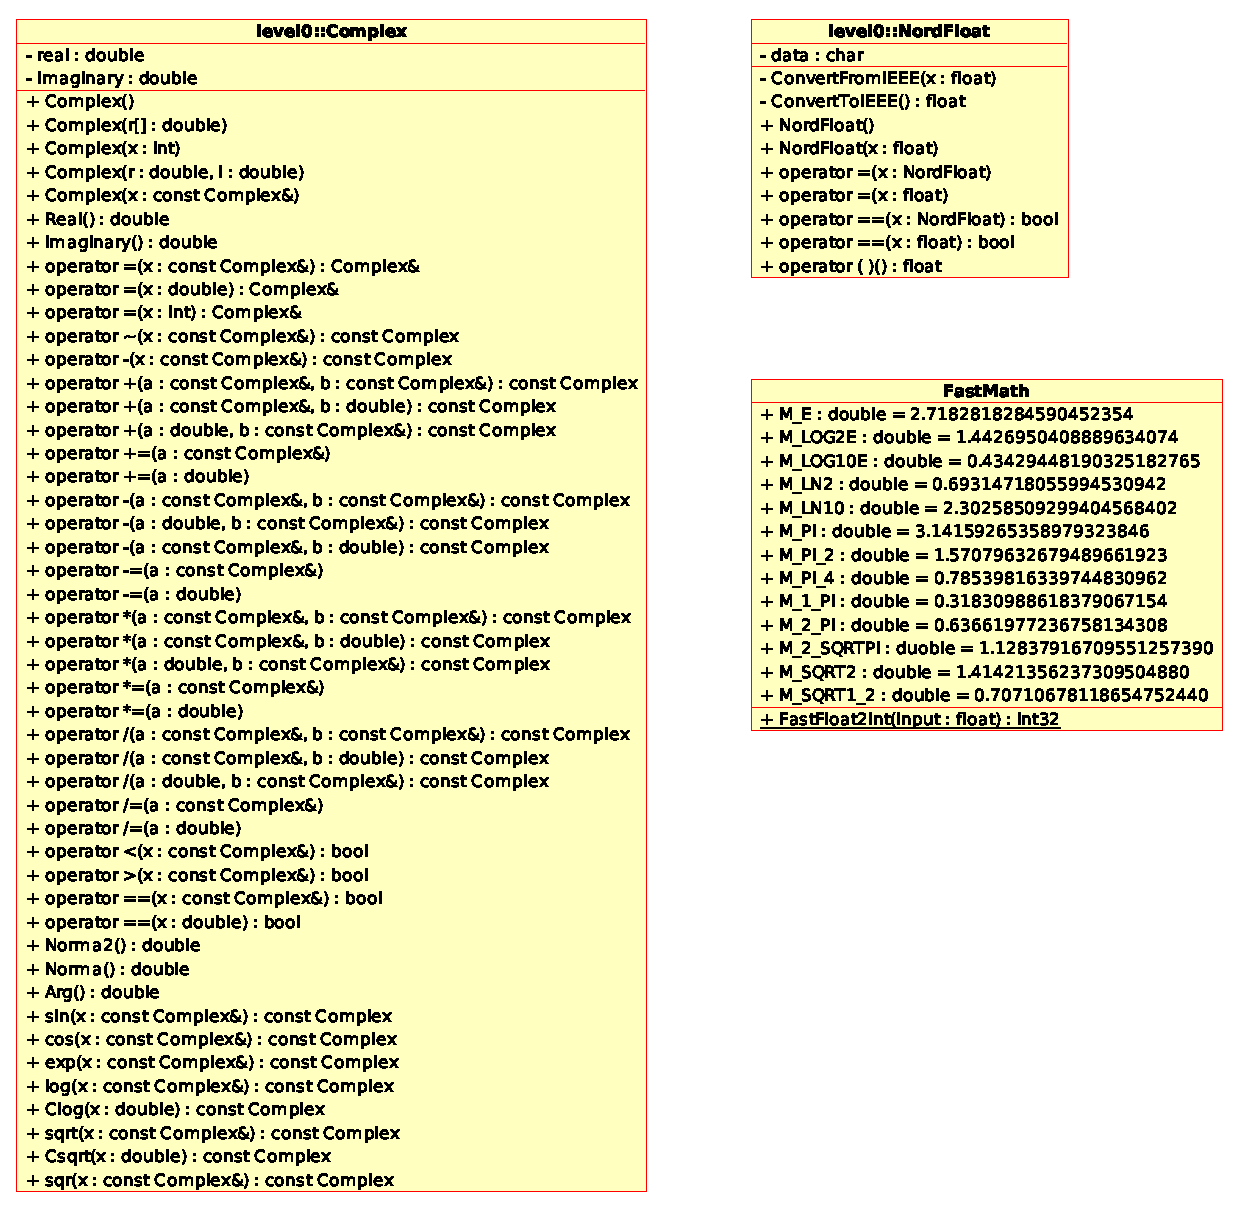
\includegraphics[width=0.73\textwidth]{level0/level0-math.eps}
  \caption{BaseLib Level0 math classes}
  \label{f:level0:math}
 \end{center}
\end{figure}



\subsubsection{Complex}
\texttt{Complex.h}\\

Comples is an implementation of the complex numerical type as 2 doubles.

The structure of the class is straightforward: it relies on two \texttt{double} attributes: \texttt{real} that holds the real part of the complex number and \texttt{imaginary} that holds the imaginary part of the complex number. There are some contructors; the first one takes no arguments, the second and third take only one argument:the real part (\texttt{double} and \texttt{int}), fourth and fifth take two doubles as the real and imaginary parts, last constructor is the copy constructor. 

There are two set methods \texttt{Real} that return the real part of the number and \texttt{Complex} that return the complex part.

\begin{lstlisting}[
extendedchars=true,%
basicstyle=\fontfamily{pcr}\fontseries{m}\selectfont\footnotesize, %
stepnumber=1,%
numberstyle=\tiny,%
keywordstyle=\footnotesize\tt ,%
language=C++]
private:
   double real;
   double imaginary;
public:
   inline Complex();
   inline Complex(double x);
   inline Complex(int x);
   inline Complex(double r,double i);
   inline Complex(double r[2]);

   inline Complex (const Complex &x);

   inline double Real();
   inline double Imaginary();
\end{lstlisting}

The class redefine all the mathematical operators using complex numbers. \texttt{operator~} return the complex conjugate of the number.

\begin{lstlisting}[
extendedchars=true,%
basicstyle=\fontfamily{pcr}\fontseries{m}\selectfont\footnotesize, %
stepnumber=1,%
numberstyle=\tiny,%
keywordstyle=\footnotesize\tt ,%
language=C++]
   inline Complex& operator=(const Complex &x);
   inline Complex& operator=(double x);
   inline Complex& operator=(int x);

   inline friend const Complex operator~(const Complex &x);
   inline friend const Complex operator-(const Complex &x);
   inline friend const Complex operator+(const Complex &a,const Complex &b);

   inline friend const Complex operator+(const Complex &a,double b);
   inline friend const Complex operator+(double a,const Complex &b);

   inline void operator+=(const Complex &a);
   inline void operator+=(double a);

   inline friend const Complex operator-(const Complex &a,const Complex &b);
   inline friend const Complex operator-(double a,const Complex &b);
   inline friend const Complex operator-(const Complex &a,double b);

   inline void operator-=(const Complex &a);
   inline void operator-=(double a);

   inline friend const Complex operator*(const Complex &a,const Complex &b)
   inline friend const Complex operator*(const Complex &a,double b);
   inline friend const Complex operator*(double a,const Complex &b);

   inline void operator*=(const Complex &a);
   inline void operator*=(double a);

   inline friend const Complex operator/(const Complex &a,const Complex &b);
   inline friend const Complex operator/(const Complex &a,double b);
   inline friend const Complex operator/(double a,const Complex &b);

   inline void operator/=(const Complex &a);
   inline void operator/=(double a);
   inline bool operator< (const Complex &x);
   inline bool operator> (const Complex &x);
   inline bool operator== (const Complex &x);
   inline bool operator== (double x);
\end{lstlisting}

There are also a set of simple mathematical functions. \texttt{Norma2} returns the norma squared, \texttt{Norma} return the norma and \texttt{Arg} return the argument (?).

\begin{lstlisting}[
extendedchars=true,%
basicstyle=\fontfamily{pcr}\fontseries{m}\selectfont\footnotesize, %
stepnumber=1,%
numberstyle=\tiny,%
keywordstyle=\footnotesize\tt ,%
language=C++]
   inline friend const Complex sin(const Complex &x);
   inline friend const Complex cos(const Complex &x);
   inline friend const Complex exp(const Complex &x);
   inline friend const Complex log(const Complex &x);
   inline friend const Complex Clog(double x);
   inline friend const Complex sqrt(const Complex &x);
   inline friend const Complex Csqrt(double x);
   inline friend const Complex sqr(const Complex &x);

   inline double Norma2()const;
   inline double Norma()const;
   inline double Arg()const;
\end{lstlisting}



\subsubsection{NordFloat}
\texttt{NordFloat.h}\\
Class \texttt{NordFloat} converts a float between network byte order (\textit{Nord}) and Intel byte order. There is only one attribute: \texttt{data} that is a \texttt{char[6]} array; there are two private methods that address the conversion between formats. There are constructors one zero constructor and one constructor that takes a \texttt{float}. Some operators are also defined.

\begin{lstlisting}[
extendedchars=true,%
basicstyle=\fontfamily{pcr}\fontseries{m}\selectfont\footnotesize, %
stepnumber=1,%
numberstyle=\tiny,%
keywordstyle=\footnotesize\tt ,%
language=C++]
private:
   char data[6];

   void ConvertFromIEEE(float x);
   float ConvertToIEEE();
public:
    NordFloat();
    NordFloat(float x);

    void operator=(NordFloat x);
    void operator=(float x);
    bool operator==(NordFloat x);
    bool operator==(float x);
    float operator()();
\end{lstlisting}



\subsubsection{FastMath}
\texttt{FastMath.h}\\
Source \textit{FastMath.h} doesn't define a class but for illustrative needes it is represented like a class in Figure \ref{f:level0:math}. The file contains one function definition and many mathematical constants. Function \texttt{FastFloat2Int} converts a float to an integer using processor instructions (will be moved in \textit{arch/}.

\begin{lstlisting}[
extendedchars=true,%
basicstyle=\fontfamily{pcr}\fontseries{m}\selectfont\footnotesize, %
stepnumber=1,%
numberstyle=\tiny,%
keywordstyle=\footnotesize\tt ,%
language=C++]
static inline int32 FastFloat2Int(float input);
\end{lstlisting}

Constants follow in Table \ref{t:math:constants}

\begin{table}[!h]
 \begin{center}
  \begin{tabular}{lll}
    $e$ & \texttt{M\_E} & 2.7182818284590452354 \\
    $log2(e)$ & \texttt{M\_LOG2E} & 1.4426950408889634074 \\
    $log10(e)$ & \texttt{M\_LOG10E} & 0.43429448190325182765 \\
    $log(2)$ & \texttt{M\_LN2} & 0.69314718055994530942 \\
    $log(10)$ & \texttt{M\_LN10} & 2.30258509299404568402 \\
    $pi$ & \texttt{M\_PI} & 3.14159265358979323846 \\
    $pi/2$ & \texttt{M\_PI\_2} & 1.57079632679489661923 \\
    $pi/4$ & \texttt{M\_PI\_4} & 0.78539816339744830962 \\
    $1/pi$ & \texttt{M\_1\_PI} & 0.31830988618379067154 \\
    $2/pi$ & \texttt{M\_2\_PI} & 0.63661977236758134308 \\
    $2/sqrt(pi)$ & \texttt{M\_2\_SQRTPI} & 1.12837916709551257390 \\
    $sqrt(2)$ & \texttt{M\_SQRT2} & 1.41421356237309504880 \\
    $sqrt(1/2)$ & \texttt{M\_SQRT1\_2} & 0.70710678118654752440 \\
   \end{tabular}
   \end{center}
  \caption{constants in \texttt{FastMath}}
 \label{t:math:constants}
\end{table}



\subsection{Design Notes}
The aim of class \texttt{NordFloat} is not really clear; probably the conversion is not between float in differents byte format. The design is ok also if there are no links between classes. Probably the class \texttt{FastMath} must moved to arch because is architecture dependent. See as an example
\begin{verbatim}
http://www.dmh2000.com/cpp/dswap.shtml
\end{verbatim}


\section{Design Notes}
In BaseLib the support to different operating systems as well as the support of different architectures is done by using the pragma def statement, this is today considered as a poor designing choice, difficult to mantain, not easy to scale and also not easy to understand. A better solution would be to adopt the same scheme adopted in the Linux kernel directory \textit{arch/}. \\



 \chapter{BaseLib Level 1}
\chaptermark{Level 1}

BaseLib Level1 group togheter differents BaseLib data structures that are vital for each application developed on the library. The first component this chapter deal with is the \textit{Object Registry Database} (ORDB) a data structure that let the user query about the run time type identification of an object (something similar with the C++'s RTTI infrastructure addressed below).
Another really usefull infrastructure is the \textit{Global Object Database} (GODB) a database structure that holds a reference to each instantiated class and also let it be garbage collectable. An \textit{Error System Instruction} is partially introduced as a linked list stucture. In Level1 you are going to see for the first time the foundamental \textit{Configuration Database}, a tree data structure that holds the most important information for the loading and configuration of the system. In such level it also possible to find the file \texttt{StreamAttributes.h} that defines some attributes that concern streams, such file will be not addressed in the following.


Classes in BaseLib Level1 can be grouped with the following criteria:
\begin{itemize}
 \item Object Registry DataBase (ORDB)
 \item Global Object DataBase (GODB)
 \item Error System Instruction (ESI)
 \item Configuration DataBase (CDB)
 \item Stream Attributes
\end{itemize}
Such groups cover all BaseLib Level 1 classes, we start analysing the first group.



\section{Object Registry DataBase}
Before starting to introduce the Object Registry DataBase structure we spend some words trying to create a general basic knowledge about Object Oriented Languages and Run Time Type Identification. RTTI, i.e. Run-Time Type Information, or Run-Time Type Identification, refers to a C++ system that keeps information about an object's data type in memory at runtime. Run-time type information can apply to simple data types, such as integers and characters, or to generic objects. This is a C++ implementation of a more generic concept called reflection.



\subsection{RTTI}

Run Time Type Identification provides some information about objects at run time such as the name of its type. The C++ language has RTTI support, which fulfills the minimal requirements, but it is not enough for many applications of RTTI, such as object persistency. Other languages (like Java and C\#) have better RTTI system making possible to declare properties for accessing the objects and the language implements also persistency (serialization in Java), but these languages have other disadvantages.

C++ programs may also need persistency and the advanced features of RTTI systems. The C++ language is so powerful that it is possible to implement properties and an advanced RTTI system.\\


The standard C++ provides the \texttt{typeid()} operator for getting type information. Its argument is an expression (a reference or a pointer of an object) or a type name. It returns a constant reference to a \texttt{type\_info} object containing some information of the object's type.

The \texttt{type\_info} class has only a few member functions:
\begin{lstlisting}[
extendedchars=true,%
basicstyle=\fontfamily{pcr}\fontseries{m}\selectfont\footnotesize, %
stepnumber=1,%
numberstyle=\tiny,%
keywordstyle=\footnotesize\tt ,%
language=C++]
class type_info {
public:
  virtual ~type_info();
  bool operator== (const type_info& rhs) const;
  bool operator!= (const type_info& rhs) const;
  bool before (const type_info& rhs) const;
  const char* name() const;
private:
  type_info (const type_info& rhs);
  type_info& operator= (const type_info& rhs);
};
\end{lstlisting}

The method \texttt{name} gets the string representation of the type (e.g. \texttt{int}, or \texttt{MyClass}); \texttt{before} is used for ordering; \texttt{operator==()} and \texttt{operator!=()} for comparing \texttt{type\_info} objects; this information does not help to find the relations of objects and does not solve most of the problems that arise in applications. It is not designed for that. All applications have different requirements and the same standard type description cannot fulfill all the requirements. \\


However the \texttt{type\_info} class can be used as a key in a map storing more detailed type information [Strousstrup 15.4.4]. This way every application can define and use its own RTTI system, which is a very flexible solution. The problem is, that someone has to define the structure of the RTTI record and fill the map with records for every type. This job is not trivial and some code has to be written for every application for doing that. \\


An alternative to this problem could be to write a piece of code able to walk the RTTI structure builded by the C++ compiler. RTTI data structures are necessary at run time for the \textit{dynamic cast} process; but what happens is that every compiler, developed from different companies, has its own data structures that differ from product to product. Using such strategy it is possible to exploit compile time produced data structures without creating your own data structures, i.e. having two parallels RTTI tables. \\



\subsection{ORDB}
BaseLib addresses the problem of knowing every class in the system holding an ORDB that is a simple linked list of all class types loaded in the system. There is only one instance of an ORDB (of type \texttt{ObjectRegistryDataBase}) at runtime and is called \texttt{ObjectRegistryDataBaseInstance} (see file \textit{level1/ObjectRegistryDataBase.cpp}). \\


The ORDB doesn't hold the hierarchy relationship between classes but it's only a list of all class types registered in the system, this list can be searched for a class by name or by an id number and it is possible to retrieve the name address of the class and other usefull informations. The whole structure of all classes that makes the ORDB work is depicted in Figure \ref{f:level1:object} that follows.

\begin{figure}[h!]
 \begin{center}
  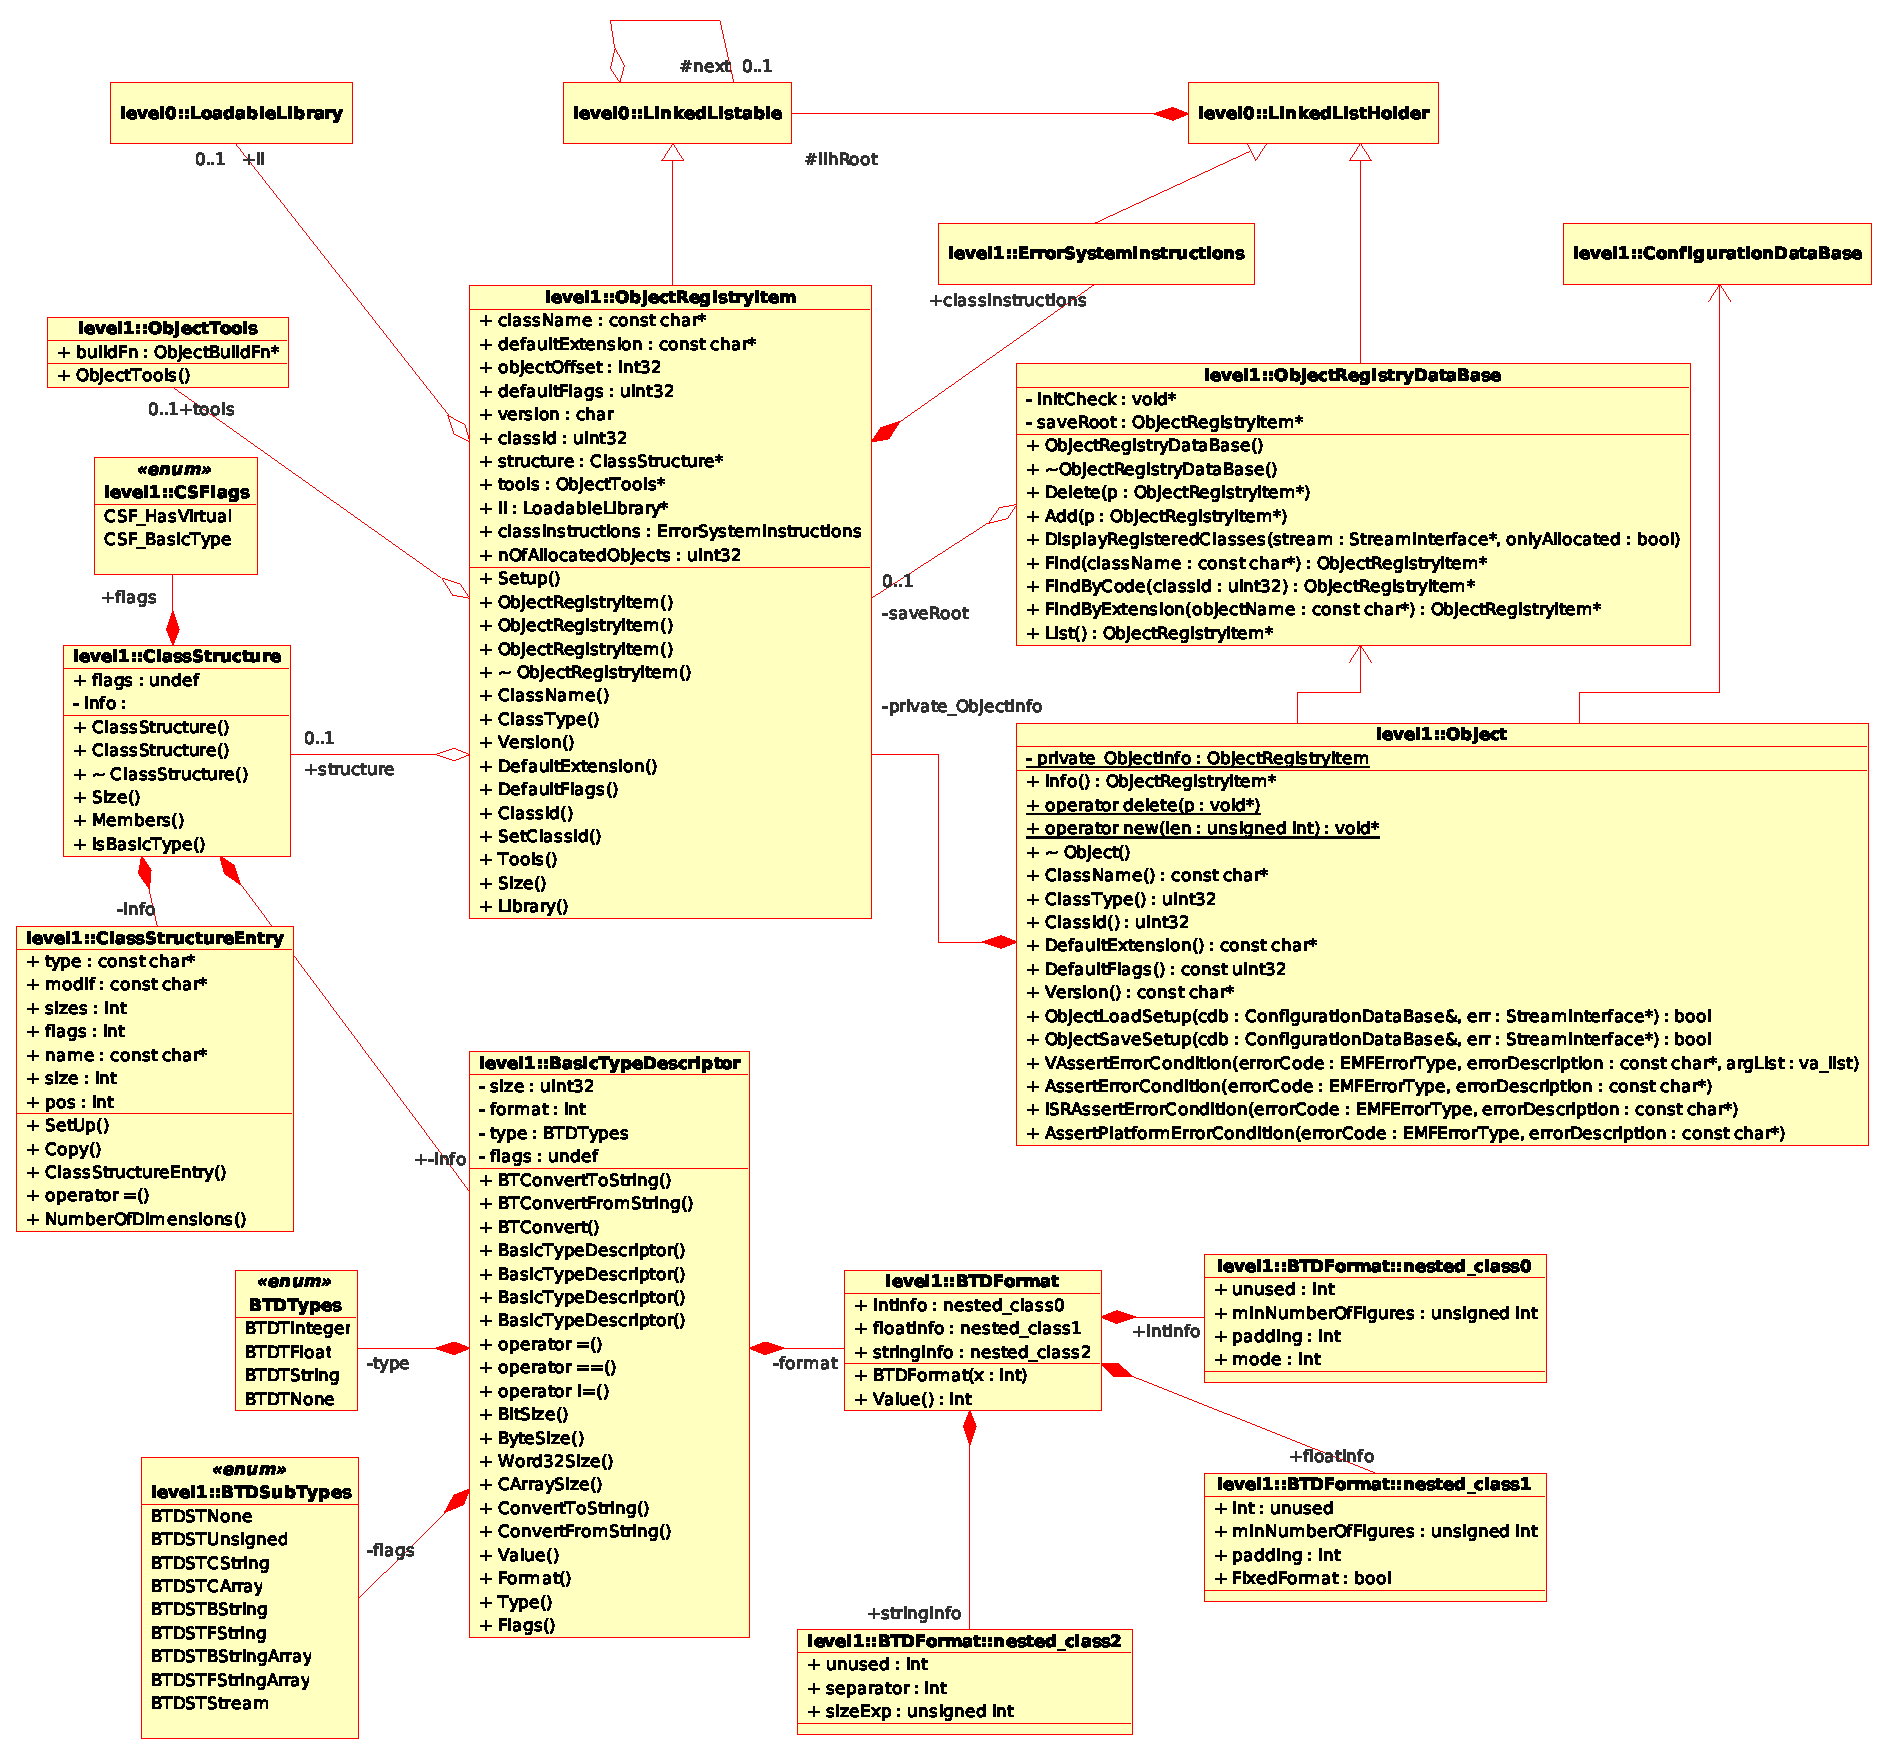
\includegraphics[width=\textwidth]{level1/level1-object.eps}
  \caption{BaseLib Level1 Object Registry Database (ORDB) classes}
  \label{f:level1:object}
 \end{center}
\end{figure}

Classess that belong to this group are:
\begin{itemize}
 \item ClassStructureEntry
 \item ClassStructure

 \item BasicTypeDescriptor
 \item BTDFormat

 \item ObjectRegistryItem, ObjectTools
 \item ObjectRegistryDataBase
 \item Object
\end{itemize}

All classes listed above estabilsh the \textit{Object Registry Database} structure. The basic idea behind this work is to imitate what is developed in the Java language: every object inherit from the \texttt{Object} class providing a common ancestor of every object that force to have some common methods (like \texttt{ToString} in Java).
In BaseLib we want to achieve the same common ancestor letting all the objects inheriting common methods and common functionalities like the most important one: be part of the ORDB. Such ORDB can be easily walked by any other object providing debbugging functionalities and runtime linking and loading. \\


We first go throught the implementation of the \texttt{ObjectRegistryDataBase} and then we show how the class \texttt{Object} can take advantage of it and which basic methods add to any other objects that inherith from that. We start with some utility classes.



\subsubsection{BTDFormat}
\texttt{[BasicTypes.h]}\\
Class \textbf{BTDFormat} is declared as a \texttt{union} with a constructor and a single method \texttt{Value}. Attribute can be a \texttt{struct intInfo}, \texttt{struct floatInfo} or \texttt{struct stringInfo}. Each struct, that follows, try to describe the format of a single basic type that can be \textit{integer}, \textit{float} or \textit{string}. The format of the \texttt{BTDFormat} depends on the endianity so that to fit in the 14 bit space in the \textbf{BasicTypeDescriptor} attribute's \texttt{format} analized in the next section.

\begin{lstlisting}[
extendedchars=true,%
basicstyle=\fontfamily{pcr}\fontseries{m}\selectfont\footnotesize, %
stepnumber=1,%
numberstyle=\tiny,%
keywordstyle=\footnotesize\tt ,%
language=C++]
union BTDFormat {
   struct {
      unsigned int minNumberOfFigures:5;
      int padding:3;
      int mode:3;
      int unused: 21;
   } intInfo;
   struct {
      unsigned int minNumberOfFigures:5;
      int padding:3;
      bool fixedFormat:1;
      int unused: 23;
   }floatInfo;
   struct {
      int separator:3;
      unsigned int sizeExp:4;
      int unused: 25;
   } stringInfo;

   BTDFormat(int x=0);
   int Value();
};
\end{lstlisting}

\texttt{intInfo} is used in single strings and streams, \texttt{floatInfo} is used in floats to determine how many meaningful figures are there and \texttt{stringInfo} is used in strings of C ARRAYs and BSTRING type.



\subsubsection{BasicTypeDescriptor}
\texttt{[BasicTypes.h, BasicTypes.cpp]}\\

Support for basic types of built in language types. Each basic type is described in BaseLib with a \texttt{BasicTypeDescriptor}, such class has the following attributes that account about the size of the object, attribute \texttt{size}, maximum size is 1024 units (10 bit), the format and type.

\begin{lstlisting}[
extendedchars=true,%
basicstyle=\fontfamily{pcr}\fontseries{m}\selectfont\footnotesize, %
stepnumber=1,%
numberstyle=\tiny,%
keywordstyle=\footnotesize\tt ,%
language=C++]
private:
   uint32 size:10;
   int format:14;
   BTDTypes type:4;
   BTDSubTypes flags:4;
\end{lstlisting}

Actually a \texttt{BasicTypeDescriptor} describes a basic type with a \texttt{type} and a \texttt{subtype}, so we have a two level description. The first level (\texttt{enum BTDTypes}) discriminate about:
\begin{itemize}
 \item \texttt{BTDTInteger}, an integer;
 \item \texttt{BTDFloat}, standard float;
 \item \texttt{BTDString}, any type of string;
 \item \texttt{BTDTNone} that's denote not a \texttt{BTDType};
\end{itemize}

For some of that specifiers there is a more precise description thanks to the \texttt{enum BTDSubType}, note that in the source code there is no \texttt{enum BTDSubType} but can be a good idea to make it. The \texttt{BTDSubType flag} define the meaning of the \texttt{size} attribute.
\begin{itemize}
 \item \texttt{BTDSTNone} no flags;
% FLAGS relative to BTDTInteger
 \item \texttt{BTDSTUnsigned} modifier for the integer;
% FLAGS relative to BTDTString
 \item \texttt{BTDSTCString} the \texttt{void*} is casted to \texttt{char**}; it's assumed to be a vector of pointers of \texttt{size} matching     that of the source, when used as destination the existing pointer is first freed and then replaced with a new malloced one;
 \item \texttt{BTDSTCArray} \texttt{char[]}, \texttt{size} field is the array size, the string is always 0 terminated;
 \item \texttt{BTDSTBString} \texttt{BString} class, \texttt{size} field is meaningless \texttt{void*} is \texttt{BString*} it is a pointer to a single \texttt{BString} the parts will be separarted using the character specified in the format field;
 \item \texttt{BTDSTFString} \texttt{FString} class, \texttt{size} field is meaningless \texttt{void*} is \texttt{FString*} it is a pointer to a single \texttt{FString} the parts will be separated using the character specified in the format field;
 \item \texttt{BTDSTBStringArray} \texttt{BString} class, \texttt{size} field is meaningless \texttt{void*} is \texttt{BString*} it is an array of \texttt{BString}s matching the input size;
 \item \texttt{BTDSTFStringArray} \texttt{FString} class, \texttt{size} field is meaningless \texttt{void*} is \texttt{FString*} it is an array of \texttt{FString}s matching the input size;
 \item \texttt{BTDSTStream} \texttt{StreamInterface} class, \texttt{size} field is meaningless.
\end{itemize}

A complete picture of that hierarchy is showed in Figure \ref{f:level1:BasicTypes}. It is really important to note the relationship between those types.
\begin{figure}[h!]
 \begin{center}
  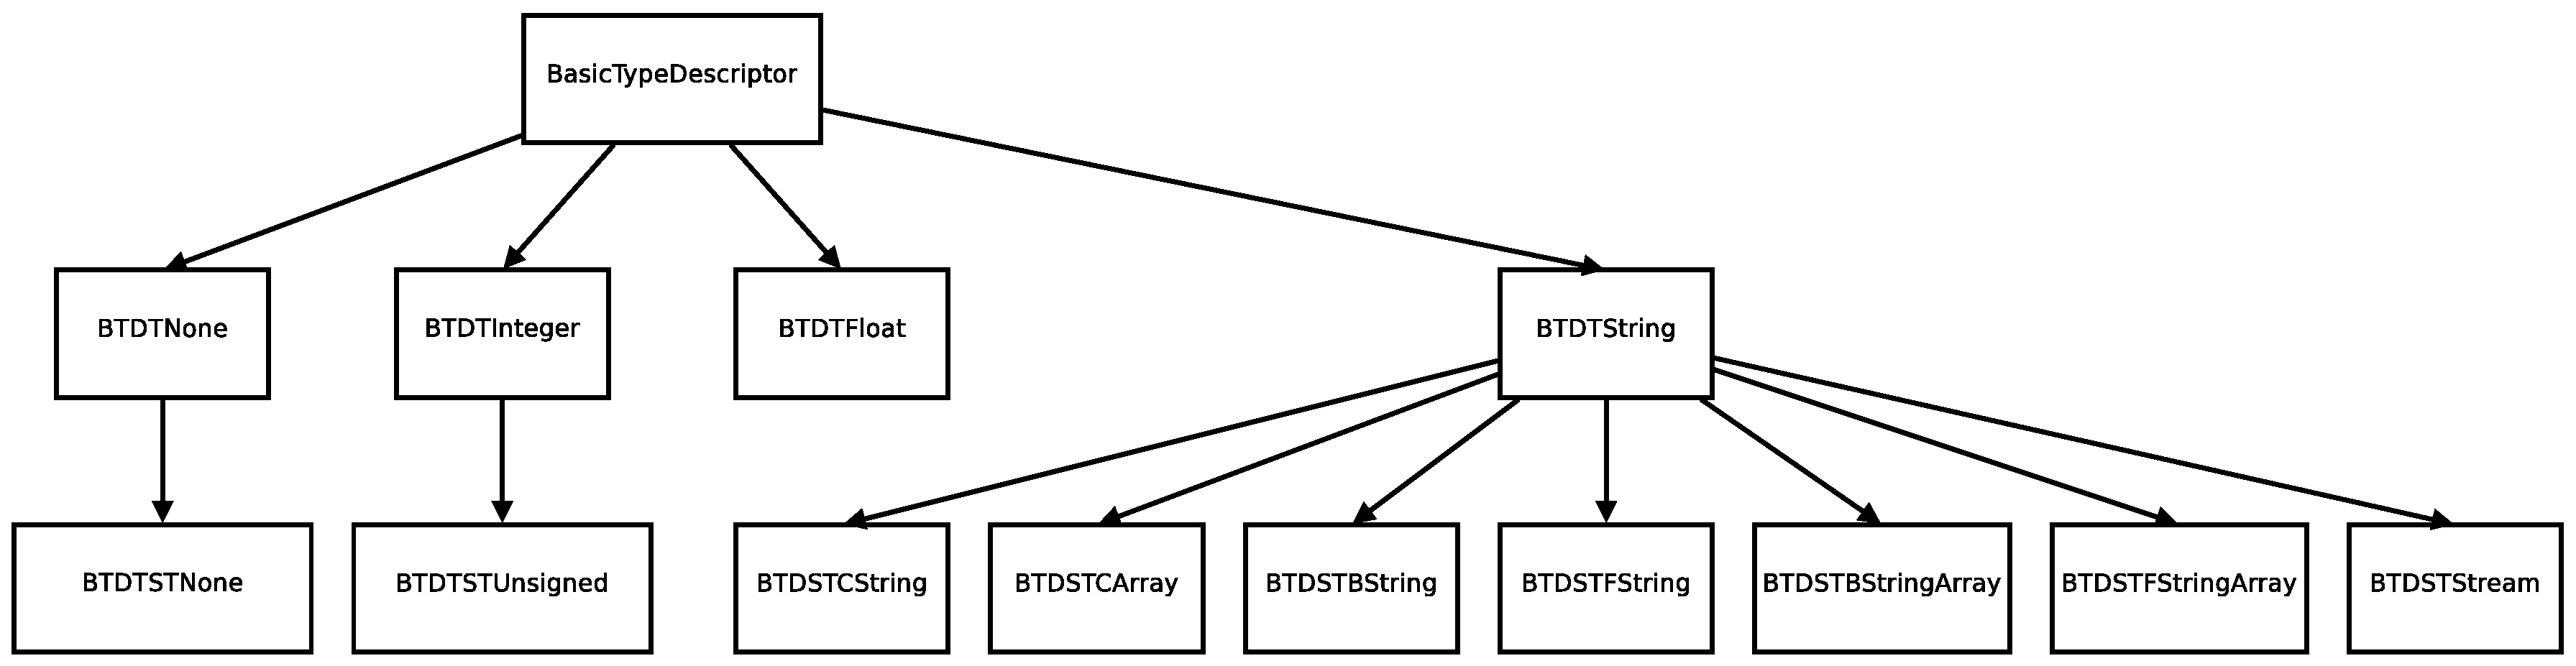
\includegraphics[width=\textwidth]{level1/types.eps}
  \caption{BaseLib Level1 BasicTypes hierarchy}
  \label{f:level1:BasicTypes}
 \end{center}
\end{figure}

Now we take a look to the methods exported from such class, there are four constructors, the first one create a \texttt{BasicTypeDescriptor} with \texttt{size} 32 bit, \texttt{type} \texttt{BTDTInteger}, \texttt{flags} \texttt{BTDSTNone} and \texttt{format} \texttt{NULL}, so it makes a \texttt{BasicTypeDescriptor} of an \textit{int32}. The second constructor helps making a new object using another one via the method \texttt{Value}. The third constructor is the most used in the library it let you construct your own basic type by setting each attribute in the class. The comes the copy constructor. \\


Then comes some getter methods that returns the size of the basic type counting the bits, bytes abd words (\texttt{BitSize}, \texttt{ByteSize} and \texttt{Word32Size} that is the minimum number of words to hold it); \texttt{CArraySize} is the size of a \texttt{CArray}. The method \texttt{Value} convert a \texttt{BasicTypeDescriptor} in an integer, \texttt{Format} return the \texttt{format} attribute, \texttt{Type} return the \texttt{type} attribute and \texttt{Flags} the \texttt{flags} attribute. \\


Methods \texttt{ConvertToString} and \texttt{ConvwertFromString} convert a string like ``uint'' in a \texttt{BasicTypeDescriptor} of type \texttt{BTDTInteger} and subtype \texttt{BTDSTUnsigned} and back.


\begin{lstlisting}[
extendedchars=true,%
basicstyle=\fontfamily{pcr}\fontseries{m}\selectfont\footnotesize, %
stepnumber=1,%
numberstyle=\tiny,%
keywordstyle=\footnotesize\tt ,%
language=C++]
public:
   BasicTypeDescriptor();
   BasicTypeDescriptor(int32 equivalent);
   BasicTypeDescriptor(uint32 size,BTDTypes type, BTDSubTypes flags,BTDFormat format = BTDFNone);
   BasicTypeDescriptor(const BasicTypeDescriptor& desc);
   BasicTypeDescriptor operator=(const BasicTypeDescriptor &desc);

   bool operator==(const BasicTypeDescriptor &desc) const;
   bool operator!=(const BasicTypeDescriptor &desc) const;

   int32 BitSize() const;
   int32 ByteSize() const;
   int32 Word32Size() const;
   uint32 CArraySize() const;

   int32 Value() const;
   BTDFormat Format() const;
   BTDTypes Type() const;
   BTDSubTypes Flags() const;

   const char* ConvertToString(BString& string) const;
   bool ConvertFromString(const char* name);
\end{lstlisting}

In the file \textit{level1/BasicTypes.h} are declared the following basic type descriptors, with the following parameters.
\begin{table}[!h]
 \begin{center}
  \begin{tabular}{|lllll|}
   \hline
type & BaseLib type & bit size & \texttt{BTDTypes} & \texttt{BTDSubTypes} \\
   \hline
8 bit signed integer & \texttt{BTDInt8} & 8 & BTDTInteger & BTDSTNone \\
16 bit signed integer & \texttt{BTDInt16} & 16 & BTDTInteger & BTDSTNone \\
32 bit signed integer & \texttt{BTDInt32} & 32 & BTDTInteger & BTDSTNone \\
64 bit signed integer & \texttt{BTDInt64} & 64 & BTDTInteger & BTDSTNone \\
8 bit unsigned integer & \texttt{BTDUint8} & 8 & BTDTInteger & BTDSTUnsigned \\
16 bit unsigned integer & \texttt{BTDUint16} & 16 & BTDTInteger & BTDSTUnsigned \\
32 bit unsigned integer & \texttt{BTDUint32} & 32 & BTDTInteger & BTDSTUnsigned \\
64 bit unsigned integer & \texttt{BTDUint64} & 64 & BTDTInteger & BTDSTUnsigned \\
32 bit float & \texttt{BTDFloat} & 32 & BTDTFloat & BTDSTNone \\
64 bit float & \texttt{BTDDouble} & 64 & BTDTFloat & BTDSTNone \\
char* string & \texttt{BTDCString} & 0 & BTDTString & BTDSTCString \\
\texttt{BString} pointer & \texttt{BTDBString} & 0 & BTDTString & BTDSTBString \\
\texttt{BString} for each element & \texttt{BTDBStringArray} & 0 & BTDTString & BTDSTBStringArray \\
\texttt{StreamInterface*} & \texttt{BTDStream} & 0 & BTDTString & BTDSTStream \\
   \hline
   \end{tabular}
   \end{center}
  \caption{\texttt{BasicTypeDescriptor}s defined in BaseLib}
 \label{t:basic_types}
\end{table}

All such types are declared \texttt{static const} and they are placed in a header file. This file is directly included in BaseLib from three \textit{*.cpp} sources and within a first indirection by other six files, so in two levels nine times, we doesn't try to recover all times that types will be recompiled in the whole BaseLib but within one level the same classes are recompiled 9 times: its a waste of memory allocate the same object privately for each compiled object.



\subsubsection{ClassStructureEntry}
\texttt{[ClassStructureEntry.h]}\\
This class describes an entry within a class structure. Each class \texttt{ClassStructureEntry} describes an attribute of the class is defining about. So each entry has a \texttt{type}, modifiers in attribute \texttt{modif} that usually are ``*'', i.e. the dereference and the reference (or address of) operator. The attribute \texttt{sizes} holds four integers, \texttt{flags} some flags, \texttt{name} is the name of the attribute we are asking for registration and \texttt{pos} is the offset between the class (extracted using \texttt{indexof}).

\begin{lstlisting}[
extendedchars=true,%
basicstyle=\fontfamily{pcr}\fontseries{m}\selectfont\footnotesize, %
stepnumber=1,%
numberstyle=\tiny,%
keywordstyle=\footnotesize\tt ,%
language=C++]
public:
   const char* type;
   const char* modif;
   int sizes[CSE_MAXSIZE];
   int flags;
   const char* name;
   int size;
   int pos;
\end{lstlisting}

The class has a \texttt{SetUp} method that is a helper constructor methods; it helps the constructor setting class's attributes, a \texttt{Copy} method that call the previous method and at the end the method \texttt{NumberOfDimensions} that count in case of an array the number of dimension of the arrays.

\begin{lstlisting}[
extendedchars=true,%
basicstyle=\fontfamily{pcr}\fontseries{m}\selectfont\footnotesize, %
stepnumber=1,%
numberstyle=\tiny,%
keywordstyle=\footnotesize\tt ,%
language=C++]
   void SetUp(const char* type,const char* modif,
      int size0,int size1,int size2,int size3,
      int flags,const char* name,
      int size,int pos);
   void Copy(ClassStructureEntry& x);

   ClassStructureEntry(const char* type="",const char* modif="",
      int size0=0,int size1=0,int size2=0,int size3=0,
      int flags=0,const char* name="",
      int size=0,int pos=0);
   ClassStructureEntry& operator=(ClassStructureEntry& x);

   int NumberOfDimensions();
\end{lstlisting}



\subsubsection{ClassStructure}
\texttt{[ClassStructure.h]}\\
The class \texttt{ClassStructure} holds information about a basic type or about a class. Class distinction is made on the attribute \texttt{flags} that is of enumeration type \texttt{CSFlags}. \\


The most important attribute of this class is the \texttt{union}; in the union it is possible to store or informations about one basic type (indexed by an \texttt{int32}) otherwise a set of \texttt{ClassStructureEntry}s. In the first case the class describe a basic type and in the last case a complete class defined by the user. In the \texttt{struct csInfo} the field \texttt{size} is the total size in bytes and \texttt{members} is a \texttt{NULL} terminated list of members.

\begin{lstlisting}[
extendedchars=true,%
basicstyle=\fontfamily{pcr}\fontseries{m}\selectfont\footnotesize, %
stepnumber=1,%
numberstyle=\tiny,%
keywordstyle=\footnotesize\tt ,%
language=C++]
public:
   CSFlags flags;
   union {
      struct {
         int32 btd;
      }btInfo;
      struct {
         int size;
         ClassStructureEntry** members;
      }csInfo;
   };
\end{lstlisting}

The first constructor builds up a \texttt{ClassStructure} object that holds a basic type, and the second builds up a class's description object of a class.

The method \texttt{size} return the size in bytes of the class, \texttt{Members} return the \texttt{csInfo.members} attribute and \texttt{IsBasicType} queries about the type of the stored object.

\begin{lstlisting}[
extendedchars=true,%
basicstyle=\fontfamily{pcr}\fontseries{m}\selectfont\footnotesize, %
stepnumber=1,%
numberstyle=\tiny,%
keywordstyle=\footnotesize\tt ,%
language=C++]
public:
   ClassStructure(const char* name,BasicTypeDescriptor btd);
   ClassStructure(const char* name,int size,CSFlags flags,ClassStructureEntry** members);
   ~ClassStructure();

   int32 Size() const;
   ClassStructureEntry** Members() const;
   bool IsBasicType(BasicTypeDescriptor &btd);
\end{lstlisting}



\subsubsection{ObjectRegistryItem, ObjectTool}
\texttt{[ObjectRegistryItem.h, ObjectRegistryItem.cpp]}\\

The first thing the file \textit{ObjectRegistryItem.h} defines is the type \texttt{ObjectBuildFn} that is a simple function type that return an \texttt{Object}.

\begin{lstlisting}[
extendedchars=true,%
basicstyle=\fontfamily{pcr}\fontseries{m}\selectfont\footnotesize, %
stepnumber=1,%
numberstyle=\tiny,%
keywordstyle=\footnotesize\tt ,%
language=C++]
typedef Object *(ObjectBuildFn)();
\end{lstlisting}

This \texttt{typedef} is used in the first class defined in the header file that is \texttt{ObjectTools}. Such class has only one attribute, public, of type \texttt{ObjectBuildFn}, the constructor let you simply set this attribute. Someone can argue about the necessity of having a class that hold a single attribute. It is not necessary infact.

\begin{lstlisting}[
extendedchars=true,%
basicstyle=\fontfamily{pcr}\fontseries{m}\selectfont\footnotesize, %
stepnumber=1,%
numberstyle=\tiny,%
keywordstyle=\footnotesize\tt ,%
language=C++]
class ObjectTools{
public:
   ObjectBuildFn* buildFn;
   ObjectTools(ObjectBuildFn* buildFn){
      this->buildFn = buildFn;
   }
};
\end{lstlisting}

Let's now spend some time on the \texttt{ObjectRegistryItem} class. This class stores information about a class type.
An \texttt{ObjectRegistryItem} save the name of the class in \texttt{className} attribute, the extension used as default in \texttt{defaultExtension}; attribute \texttt{objectOffset} is the relative position of \texttt{Object} within the class; \texttt{defaultFlags} holds some default attributes for the class; \texttt{version} holds the version string of this class.
The attribute \texttt{classId} is an user defineable class identification, the default one is calculated as a checksum of the name based on $sum(x) sum(x^2) sum(x^3) sum(x^4)$, \texttt{structure} holds information about the structure of this class; \texttt{tools} is the function to create this class; \texttt{ll} attribute maintain information about the loadable library where the class's object code resides; \texttt{classInstructions} collect all information about the behaviour on error situations. The attribute \texttt{nOfAllocatedObjects} count runtime, for each class type, how many objects of that type are instantiated in the system.

\begin{lstlisting}[
extendedchars=true,%
basicstyle=\fontfamily{pcr}\fontseries{m}\selectfont\footnotesize, %
stepnumber=1,%
numberstyle=\tiny,%
keywordstyle=\footnotesize\tt ,%
language=C++]
public:
   const char* className;
   const char* defaultExtension;
   int32 objectOffset;
   uint32 defaultFlags;
   char version[8];
   uint32 classId;
   ClassStructure* structure;
   ObjectTools* tools;
   LoadableLibrary* ll;
   ErrorSystemInstructions classInstructions;
   uint32 nOfAllocatedObjects;
\end{lstlisting}

Then follow a set of getter methods, there is a setter method only for the \texttt{classId} attribute. The method \texttt{ClassType} returns the type of the class, this identification code is unique within an application, in the actual implementation it returns value of the char pointer \texttt{className}.

\begin{lstlisting}[
extendedchars=true,%
basicstyle=\fontfamily{pcr}\fontseries{m}\selectfont\footnotesize, %
stepnumber=1,%
numberstyle=\tiny,%
keywordstyle=\footnotesize\tt ,%
language=C++]
   const char* ClassName();
   uint32 ClassType();
   const char* DefaultExtension();
   
   const uint32 DefaultFlags();
   const char* Version();

   uint32 ClassId();
   void SetClassId(uint32 id);
   ObjectTools* Tools();
   int Size();

   LoadableLibrary* Library();
\end{lstlisting}

The method \texttt{Setup} is an helper method for the constructor, argument \texttt{className} is the name of the class, \texttt{version} is the version of the class as a string (see more on next sections).
Constructors initialise the structure details of a \textit{Object Registy DataBase} record using the structure information, adding this \texttt{ObjectRegistryItem} to the database after calling the main constructor if a record of class \texttt{className} is not found  in the ORDB.

\begin{lstlisting}[
extendedchars=true,%
basicstyle=\fontfamily{pcr}\fontseries{m}\selectfont\footnotesize, %
stepnumber=1,%
numberstyle=\tiny,%
keywordstyle=\footnotesize\tt ,%
language=C++]
   void Setup(const char* className,
              const char* version,
              const char* defaultExtension = NULL,
              uint32 defaultFlags = 0,
              ObjectTools* tools = NULL);

   ObjectRegistryItem();
   ObjectRegistryItem(const char* className,
                      const char* version,
                      int objectOffset,
                      const char* defaultExtension = NULL,
                      uint32 defaultFlags = 0,
                      ObjectTools* tools = NULL);
   ObjectRegistryItem(const char* className, ClassStructure* structure);

   ~ObjectRegistryItem();
\end{lstlisting}



\subsubsection{ObjectRegistryDataBase}
\texttt{[ObjectRegistryDataBase.h, ObjectRegistryDataBase.cpp]}\\
The \textit{Object Registry Database} is the system-wide class database that take notes of every class type registered in your application; for each class type, we saw on previous section about \texttt{ObjectRegistryItem} we have a usage count.\\


The \texttt{ObjectRegistryDataBase} can be used to save and load classes creating recogniseable objects. To perform such activity the \texttt{ObjectRegistryDataBase} is of type \texttt{LinkedListHolder} and holds \texttt{ObjectRegistryItem}s. Extending the \textit{Linked List} concept it inherits the searching and filtering capability.\\


There are just two attributes, a \texttt{void*} called \texttt{initCheck} that points to itself, if not, the object is not initialized; there is also a \texttt{ObjectRegistryItem*} that keeps a copy of the pointer to the list. Note that someone can argue that this attribute is not really necessary because \texttt{ObjectRegistryDataBase} is a subclass of \texttt{LinkedListHolder} that holds an attribute of type \texttt{LinkedListable} and \texttt{ObjectRegistryItem} is a sublcass of such class. So it is simply a matter of casting the \texttt{ObjectRegistryDataBase::llhRoot} element to a \texttt{ObjectRegistryItem}.

\begin{lstlisting}[
extendedchars=true,%
basicstyle=\fontfamily{pcr}\fontseries{m}\selectfont\footnotesize, %
stepnumber=1,%
numberstyle=\tiny,%
keywordstyle=\footnotesize\tt ,%
language=C++]
   void* initCheck;
   ObjectRegistryItem* saveRoot;
\end{lstlisting}

The constructor during initialization wipes the list since this object could be initialized later than it was used, a trick had to be used, if the list has been already initialized then recover the lost list. All the methods are aimed at allowing insertion to the list even if it has not been yet initialized, the top of the list is saved continuously. Methods \texttt{Delete} and \texttt{Add} lets you delete and add an \texttt{ObjectRegistryItem} to the database.

The method \texttt{Find} search a class using the \texttt{className} passed by argument in the loaded loadable libraries in the system. First it checks against the syntax of the request and than scan to search the library.
Other find methods search a class by an identification or by the full object file name or just its extension. The method \texttt{List} return back the complete list of \texttt{ObjectRegistryItem} objects.

\begin{lstlisting}[
extendedchars=true,%
basicstyle=\fontfamily{pcr}\fontseries{m}\selectfont\footnotesize, %
stepnumber=1,%
numberstyle=\tiny,%
keywordstyle=\footnotesize\tt ,%
language=C++]
public:
   ObjectRegistryDataBase();
    ~ObjectRegistryDataBase();

   void Delete(ObjectRegistryItem* p);
   void Add(ObjectRegistryItem* p);

   void DisplayRegisteredClasses(StreamInterface* stream,bool onlyAllocated);

   ObjectRegistryItem* Find(const char* className);
   ObjectRegistryItem* FindByCode(uint32 classId);
   ObjectRegistryItem* FindByExtension(const char* objectName);

   ObjectRegistryItem* List();
\end{lstlisting}

There is only one instance at runtime of the \texttt{ObjectRegistryDataBase} class in the system and you can look at that in the file \textit{level1/ObjectRegistryDataBase.cpp} and the name is \texttt{ObjectRegistryDataBaseInstance}.



\subsubsection{Object}
\texttt{[Object.h, Object.cpp, ObjectMacros.h]}\\
This is the standard base class providing a type information system; it needs that each subclass provides a \texttt{className} buffer and overrides both methods \texttt{Name()} and \texttt{Type()}. Every class that inherits from \texttt{Object} must have the following methods:

\begin{lstlisting}[
extendedchars=true,%
basicstyle=\fontfamily{pcr}\fontseries{m}\selectfont\footnotesize, %
stepnumber=1,%
numberstyle=\tiny,%
keywordstyle=\footnotesize\tt ,%
language=C++]
public:
   virtual ~Object()

   const char* ClassName() const;
   uint32 ClassType();
   uint32 ClassId();
   const char* DefaultExtension();
   const uint32 DefaultFlags();
   const char* Version();
\end{lstlisting}

Those methods lets the ORDB work infact they supply all the type information the system need. For each class objects the class's name is returned with \texttt{ClassName}, the type is returned with \texttt{ClassType}, an identification is returned using \texttt{ClassId} extension, flags and version using \texttt{DefaultExtension}, \texttt{DefaultFlags} and \texttt{Version}. All that informations are not stored inside the \texttt{Object} class, as you can see in Figure \ref{f:level1:object} but in an \texttt{ObjectRegistryItem} attribute associated with the object. Such attribute \texttt{private\_ObjectInfo} is not declared as a static attribute in the class but it's a static global object declared in the \texttt{*.cpp} code using the macros that follow.\\ 

Next two paragraphs address two BaseLib's objects from this level that are treatened in next sections, those objects are really important for mechanisms involved in this section.


\paragraph{Configuration DataBase}
A \textit{Configuration DataBase} is a sort of data structure that is the source and also the sink of configuration parameters of the library. The method \texttt{ObjectLoadSetup} is the standard \texttt{Object} creation function. Uses a CDB to pass the initialisation parameters. The CDB information is read from the subtree that is currently addressed. The method \texttt{ObjectSaveSetup} is the standard \texttt{Object} save function. Uses a CDB to save the parameters. \\


It works like this: a CDB holds all informations about classes that must be built at runtime, you load a CDB and then reading the CDB BaseLib instantiate the objects the CDB is listing for. Each \texttt{Object} subclass must also overload last two methods, in this way each subclass can read and save its own parameters in such methods.


\paragraph{Error Management}
There also some methods for error management. The method \texttt{VAssertErrorCondition} sets the error status and depending on setup does appropriate action, this call is to be called from static members; the method \texttt{AssertErrorCondition} sets the error status and depending on setup does appropriate action, such call is to be called from static members. The method \texttt{ISRAssertErrorCondition} sets the error status and depending on setup does appropriate action, this call is to be called from interrupts. \texttt{AssertPlatformErrorCondition} sets the error status and depending on setup does appropriate action.


\begin{lstlisting}[
extendedchars=true,%
basicstyle=\fontfamily{pcr}\fontseries{m}\selectfont\footnotesize, %
stepnumber=1,%
numberstyle=\tiny,%
keywordstyle=\footnotesize\tt ,%
language=C++]
   virtual bool ObjectLoadSetup(ConfigurationDataBase& cdb,StreamInterface* err);
   virtual bool ObjectSaveSetup(ConfigurationDataBase& cdb,StreamInterface* err);

   void VAssertErrorCondition(EMFErrorType errorCode,
                           const char* errorDescription,
                           va_list argList);
   void AssertErrorCondition(EMFErrorType errorCode,
                           const char* errorDescription=NULL,...) const;
   void ISRAssertErrorCondition(EMFErrorType errorCode,
                           const char* errorDescription=NULL,...);
   void AssertPlatformErrorCondition(EMFErrorType errorCode,
                           const char* errorDescription=NULL,...);
\end{lstlisting}


\paragraph{Object Macros}
If you compare the previous listing of the class's methods with the class interface in Figure \ref{f:level1:object} it is  possible to note that in our last listing there is no class's attribute and there are less methods then in the UML.

This happens because the ORDB relay on some code macros to work. All macros used throught BaseLib, concerning the ORDB are from the file \textit{level1/ObjectMacros.h}. Now we spend some words about those macros that must be used in the development of new pieces of code. We start providing an example of how that macros are used in the \texttt{Object} class just analized. In \texttt{Object}'s header file the following macros are used outside the class declaration, the first one, and the second one inside it.

\begin{lstlisting}[
extendedchars=true,%
basicstyle=\fontfamily{pcr}\fontseries{m}\selectfont\footnotesize, %
stepnumber=1,%
numberstyle=\tiny,%
keywordstyle=\footnotesize\tt ,%
language=C++]
OBJECT_DLL(Object)
OBJECT_DLL_STUFF(Object)
\end{lstlisting}

In the source file (\texttt{*.cpp}) the following macros is used:

\begin{lstlisting}[
extendedchars=true,%
basicstyle=\fontfamily{pcr}\fontseries{m}\selectfont\footnotesize, %
stepnumber=1,%
numberstyle=\tiny,%
keywordstyle=\footnotesize\tt ,%
language=C++]
OBJECTREGISTER(Object,"$Id: level1.tex,v 1.12 2009/10/16 16:45:22 abarb Exp $")
\end{lstlisting}

Figure \ref{f:level1:object_macro} depict show macro placement. We now expand it to understand better what they create improving the understanding of the library behaviour.

\begin{figure}[h!]
 \begin{center}
  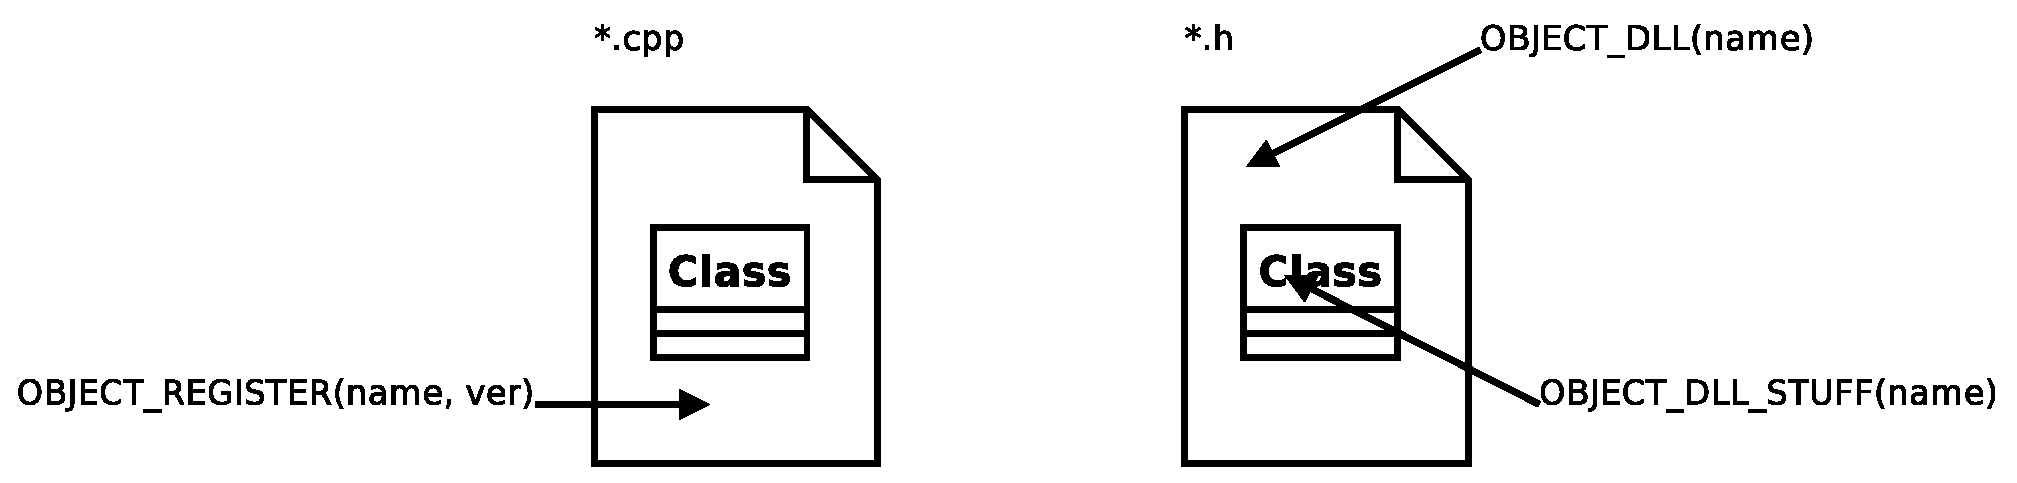
\includegraphics[width=0.77\textwidth]{level1/objectMacros.eps}
  \caption{BaseLib Level1 Object Macros position}
  \label{f:level1:object_macro}
 \end{center}
\end{figure}

The first two macros presented expand to the following code. That code redefine the class \texttt{new} and \texttt{delete} operators, provide a \texttt{Info} methods that return a \texttt{ObjectRegistryItem*} about that inform about the class type.

\begin{lstlisting}[
extendedchars=true,%
basicstyle=\fontfamily{pcr}\fontseries{m}\selectfont\footnotesize, %
stepnumber=1,%
numberstyle=\tiny,%
keywordstyle=\footnotesize\tt ,%
language=C++]
   extern "C" {
      ObjectRegistryItem* Get_private_ObjectInfo();
   }

class Object {
public:
   virtual ObjectRegistryItem* Info() const {
      return Get_private_ObjectInfo();
   }
   static void operator delete(void* p) {
      OBJDeleteFun(p,Get_private_ObjectInfo());
   }
   static void* operator new(unsigned int len) {
      return OBJNewFun(len,Get_private_ObjectInfo());
   }
   friend Object* ObjectBuildFn__ ();
\end{lstlisting}

Last macro listed expand to the following code that it is possible to find in the \texttt{*.cpp} file and is statically compiled one time. The first three row statically declare an \texttt{ObjectRegistryItem} that will be registered in the ORDB providing type information with the version information.

\begin{lstlisting}[
extendedchars=true,%
basicstyle=\fontfamily{pcr}\fontseries{m}\selectfont\footnotesize, %
stepnumber=1,%
numberstyle=\tiny,%
keywordstyle=\footnotesize\tt ,%
language=C++]
   static ObjectRegistryItem _private_ObjectInfo(Object,
      "$Id: level1.tex,v 1.12 2009/10/16 16:45:22 abarb Exp $",
      ObjectClassOffset(Object));
   ObjectRegistryItem *Get_private_ObjectInfo(){
      return &_private_ObjectInfo;
   }
\end{lstlisting}

There are also other macros in the \textit{level1/ObjectMacros.h} and are listed below. Comments are from the source code.

\begin{itemize}
\item \texttt{OBJECT\_DLL(name)} To allow registering a class contained in a DLL. Use before the class declaration outside the class
\item \texttt{OBJECT\_DLL\_STUFF(name)} To allow registering a class contained in a DLL. Use inside the class remember to set the public/private/protected afterwards.
\item \texttt{OBJECT\_STUFF(name)} To allow registering a class. Use inside the class. remember to set the public/private/protected afterwards.

\item \texttt{OBJECTREGISTER(name,ver)} Register a class with its version. Use in the \texttt{*.cpp} file
\item \texttt{OBJECTLOADREGISTER(name,ver)} Register a class with its version. Use in the \texttt{*.cpp} file. Automatically creates the Build function.
\item \texttt{OBJECTLOADREGISTERFLAGS(name,ext,flags,ver)} Register a class with its version. Use in the \texttt{*.cpp} file. Automatically creates the Build function. Sets the flags an the file extension.

\item \texttt{STRUCTREGISTER(name,structure)} Register a structure with its fields (structure). Use in the \texttt{*.cpp} file.

\item \texttt{BASICTYPEREGISTER(name,type)} Register a basic type (int float ...). Use in the \texttt{*.cpp} file.
\item \texttt{BASICTYPEREGISTER2(mod,name,type)} Register a basic type with a modifier in the name (short int long a = t ...). Use in the \texttt{*.cpp} file.
\item \texttt{BASICTYPEREGISTER3(mod,mod2,name,type )} Register a basic type with 2 modifiers in the name (short int long b=t ...).   Use in the .cpp file.
\end{itemize}



\subsection{Remarks}
TODO \\
TODO \\
TODO \\
Spiegare come sfruttare la reflection per creare una classe creare una classe via nome.



\subsection{Design Notes}
This section highlighted the basic RTTI-like functionality that BaseLib provide to the user. The ORDB presented here is a simply linked list with searching functionality. The design was made without thinking about preformance but focusing on the usability. The ORDB is really like a database, every loaded component of BaseLib as soon is loaded in the system register all class type it has and then, accessing the ORDB one can find the class it want and through the CDB loading it with the help of the ORDB. \\


At this level there is no hierical information between classes stored. So for example there is no method that tell you if a \texttt{ObjectRegistryDataBase} is a \texttt{LinkedListHolder} or not. This hierical relationship must be showed from the ORDB this can help also for the garbage collection (is it implemented in the GODB?). \\


ObjectTool is not necessary as a class: it has only one attribute can be deleted or improved.\\


The idea of having basic types and structured types is a good choice. Union's are probebly not the best choice because are rarely used in Object Oriented languages. The best design choice is to create an abstract type and subclassing it by basic types and by structured object: this is OOP (Object Oriented Programming).



\section{Global Object DataBase}
Such section address the \textit{Global Object Database} that mantain a list of all instantiated objects that registrates with them. A garbage collector mechanisms is implemented, each object that inherits from some other that is GarbageCollectable can be handled by the collector and make your work memory safe; every object that will be registered will be automatically deleted by the library, like in Java. This helps the programmer providing a way to not waste memory.

\begin{figure}[h!]
 \begin{center}
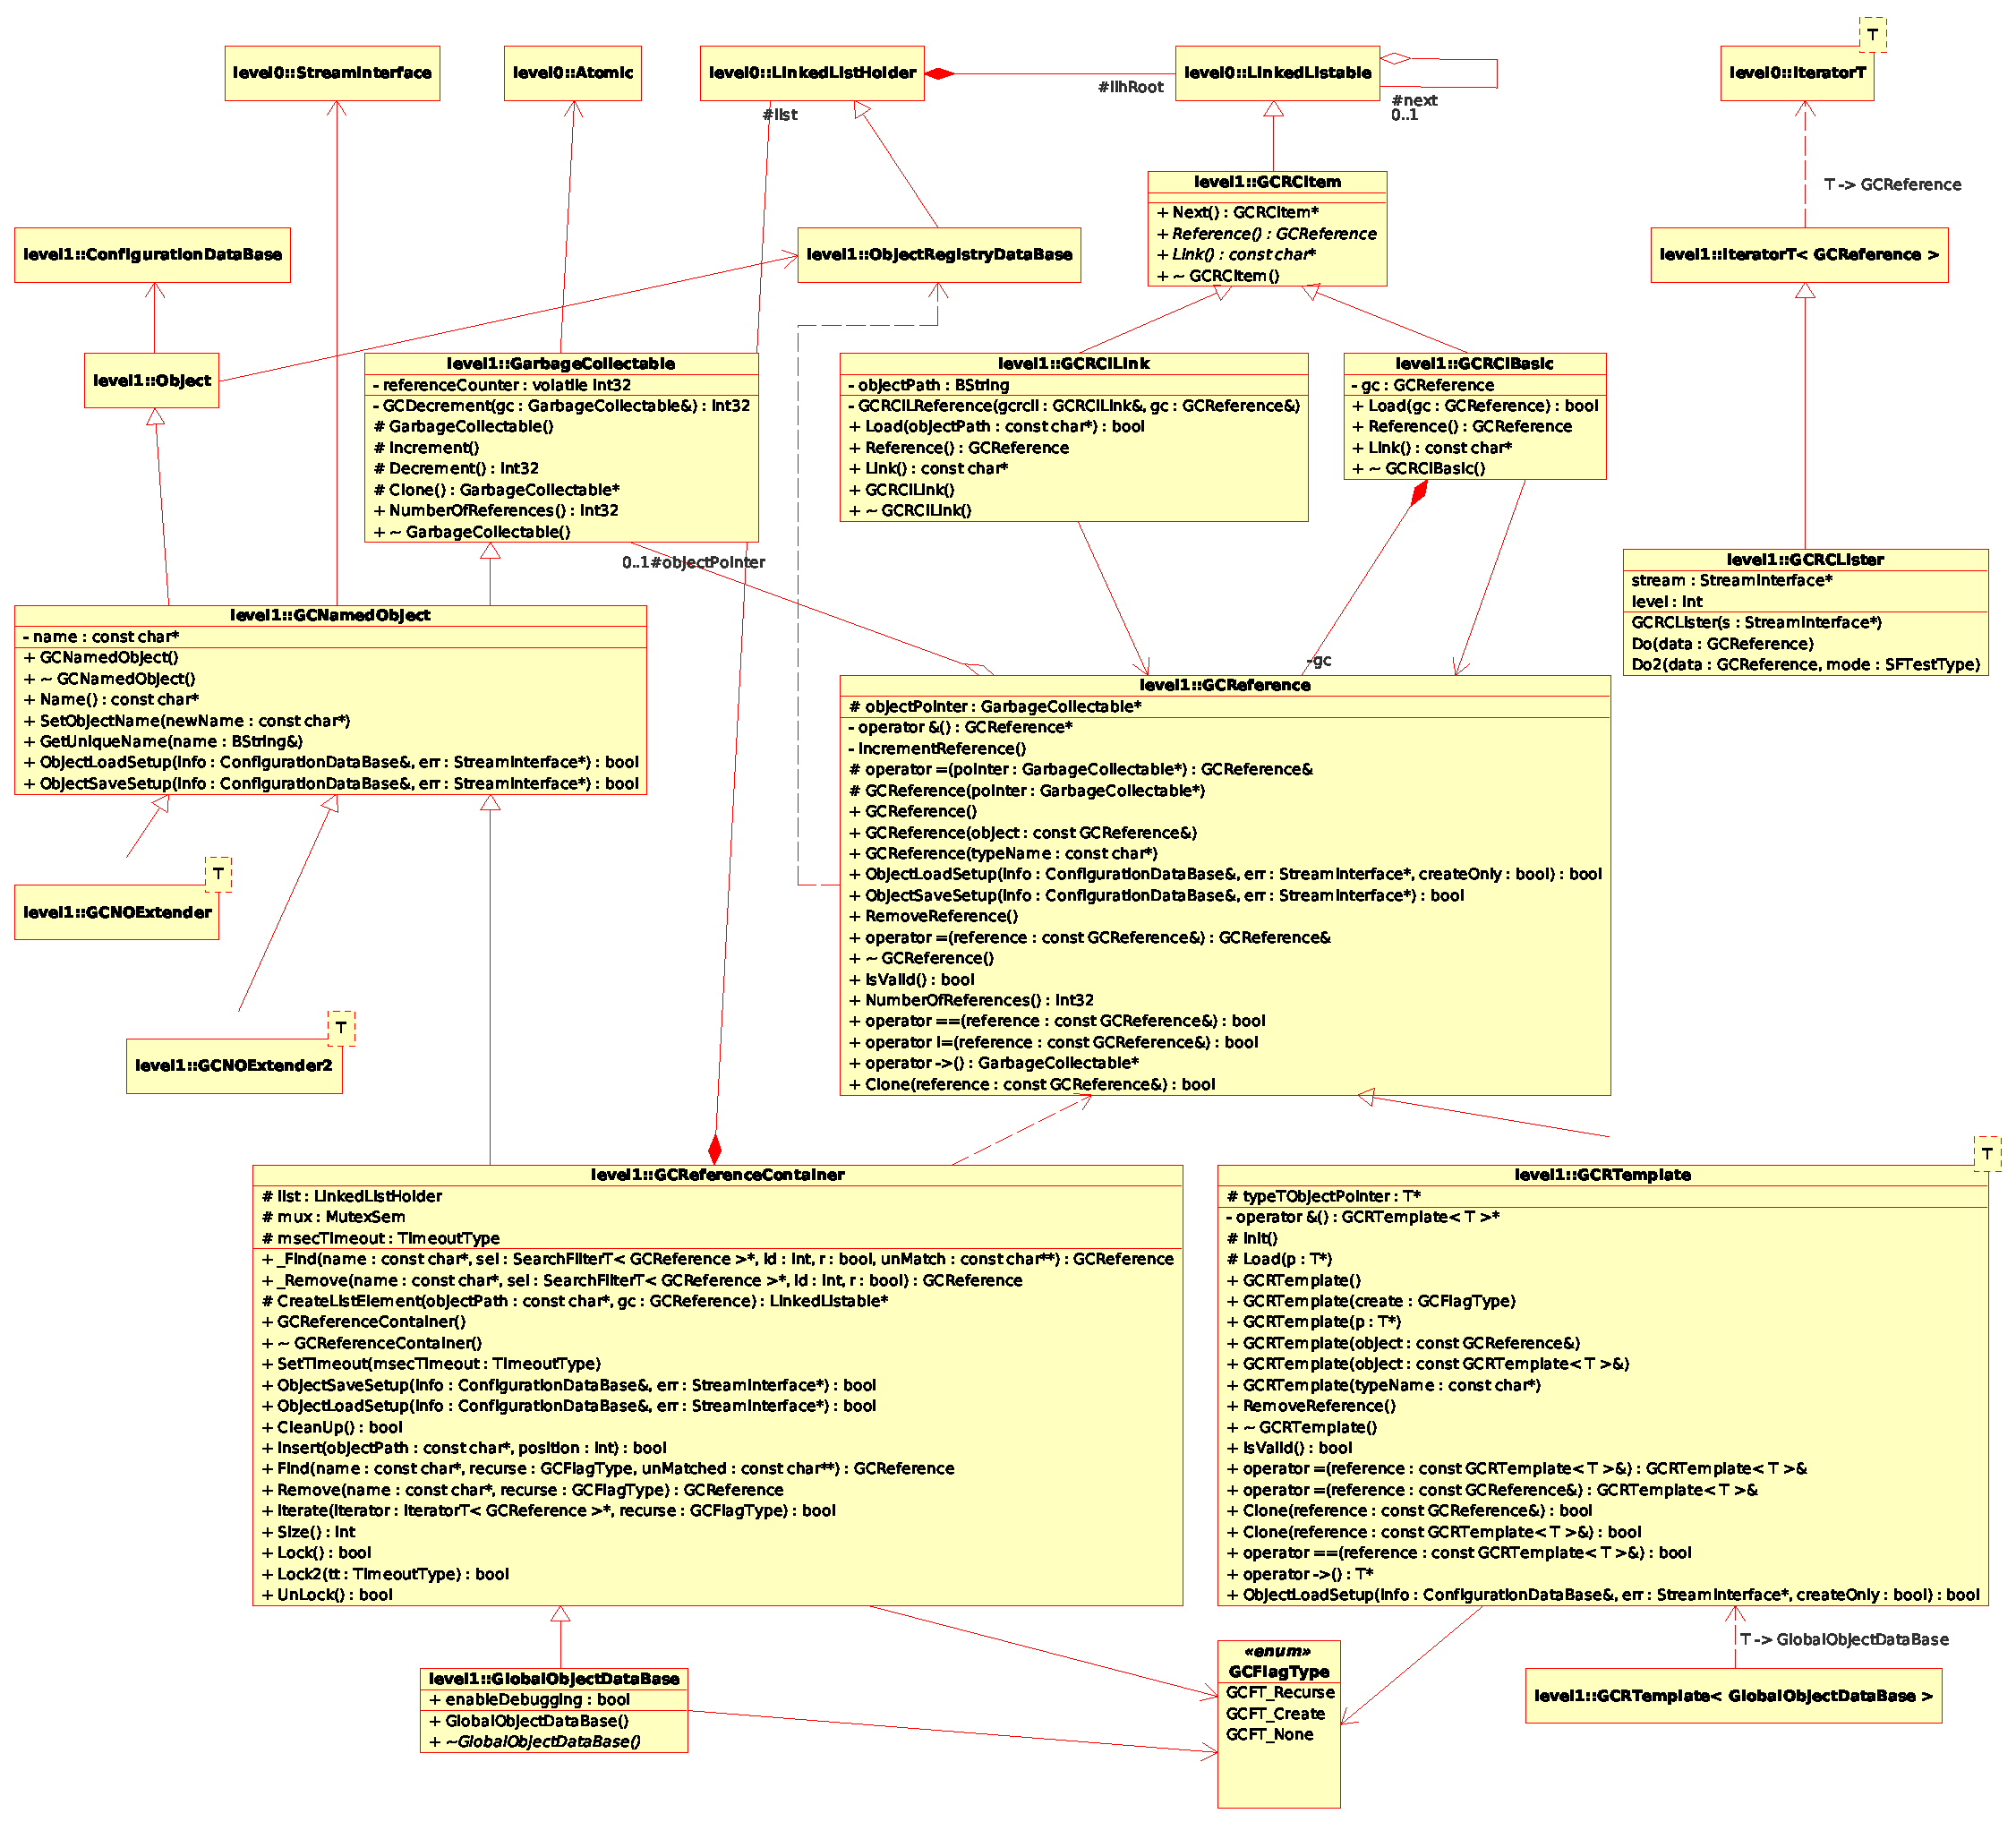
\includegraphics[width=1.1\textwidth]{level1/level1-GC.eps}
  \caption{BaseLib Level1 Global Object Database (GODB) classes}
  \label{f:level1:GC}
 \end{center}
\end{figure}

Objects of the class \texttt{GCNamedObject} inherits from \texttt{Object} but are also \texttt{GarbageCollectable}, so they are from a registered type in the ORDB but also can be collected for garbage reclaiming and within the \texttt{GCNamedObject} class they also have a name that is used to store different or the same object types in the GlobalObjectDataBase (GODB); in this way you can instantiate object by name and also reclaiming object.\\

What is the difference between an \texttt{Object} and an \texttt{GCNamedObject}? An \texttt{Object} registers in the ORDB a type of data, i.e. a class structure, a \texttt{GCNamedObject} instead register an instance of an object by name (or handle, or id). A \texttt{GCNamedObject} is also \texttt{GarbageCollectable} but an \texttt{Object} is not.\\

Classes in this section are depicted in the UML diagram of Figure \ref{f:level1:GC} and are listed below:

\begin{itemize}
 \item GarbageCollectable
 \item GCNamedObject
 \item GCNOExtender, GCNOExtender2

 \item GCRCItem, GCRCILink, GCRCIBasic
 \item GCRCLister
 \item GCReference

 \item GCRTemplate
 \item GCReferenceContainer
 \item GlobalObjectDataBase
\end{itemize}



\subsubsection{GarbageCollectable}
\texttt{[GarbageCollectable.h, GarbageCollectable.cpp]}\\
A class interface for implementing classes whose number of references is always accounted for; inherit from this class to implement garbage collection on a class. It accounts for reference to a class. It is really a simple class it provides only reference counting. \\


There is only one attribute \texttt{referenceCounter} that let supply all the functionality we need; the constructor initialises \texttt{referenceCounter} to zero, the method \texttt{Increment} is used to atomically increment the reference counter and the method \texttt{Decrement} is used to atomically decrement the reference counter.

To allow cloning of objects using references the final class must implement the method \texttt{Clone}. The method \texttt{NumberOfReferences} gets the number of references. The destructor is only called when the object is actually destroyed. The code does nothing here!

\begin{lstlisting}[
extendedchars=true,%
basicstyle=\fontfamily{pcr}\fontseries{m}\selectfont\footnotesize, %
stepnumber=1,%
numberstyle=\tiny,%
keywordstyle=\footnotesize\tt ,%
language=C++]
private:
   volatile int32 referenceCounter;
protected:
   GarbageCollectable();

   void Increment();
   int32 Decrement();

   virtual GarbageCollectable* Clone() const;
public:
   int32 NumberOfReferences() const;
   virtual ~GarbageCollectable();
\end{lstlisting}



\subsubsection{GCNamedObject}
\texttt{[GCNamedObject.h, GCNamedObject.cpp]}\\
A \texttt{GCNamedObject} is an extension of the \texttt{Object} class to include garbage collection and naming. It is used later to store object in the \texttt{GlobalObjectDataBase}.

A \texttt{GCNamedObject} is an \texttt{Object}, so it's class type will be registered, and it is also garbage collectable, so also it's usage is supervised and if it is not used jet it will be eliminated.\\


There is only one attribute \texttt{name} that adds to the \texttt{Object} a name string that will be necessary to identify it and so it must always contains a valid pointer to allocated memory. The constructor initialise to no name and the destructor deallocates memory.
The method \texttt{Name} accesses the name, \texttt{SetObjectName} sets the name and \texttt{GetUniqueName} returns a name that contains also the address, it begins with \textit{(address)name}.

The method \texttt{ObjectLoadSetup} initialises the name of the object using a CDB object, if \texttt{Name} is found than the name is taken from there, if missing then the \texttt{nodeName} is used, if \texttt{nodeName} start with \texttt{+} then the\texttt{ +} is removed (after reading the stuff about CDB you will better understand those comments). \texttt{ObjectSaveSetup} saves the settings in the CDB passed by argument.

\begin{lstlisting}[
extendedchars=true,%
basicstyle=\fontfamily{pcr}\fontseries{m}\selectfont\footnotesize, %
stepnumber=1,%
numberstyle=\tiny,%
keywordstyle=\footnotesize\tt ,%
language=C++]
private:
   const char* name;
public:
   GCNamedObject();
   virtual ~GCNamedObject();

   const char* Name()const;
   void SetObjectName(const char* newName);
   void GetUniqueName(BString& name);

   virtual bool ObjectLoadSetup(ConfigurationDataBase& info,
      StreamInterface* err);
   virtual bool ObjectSaveSetup(ConfigurationDataBase& info,
      StreamInterface* err);
\end{lstlisting}



\subsubsection{GCNOExtender, GCNOExtender2}
\texttt{[GCNOExtender.h]}\\
The following templates creates classes that are joint \texttt{GCNamedObject} and user defined class, used to add \texttt{GarbageCollection} and naming to existing classes. The first template is really simple: it creates a new class that inherits from \texttt{GCNamedObject} and the templatized class without adding any method.

\begin{lstlisting}[
extendedchars=true,%
basicstyle=\fontfamily{pcr}\fontseries{m}\selectfont\footnotesize, %
stepnumber=1,%
numberstyle=\tiny,%
keywordstyle=\footnotesize\tt ,%
language=C++]
template <class T>
class GCNOExtender: public GCNamedObject, public T
{
public:

};
\end{lstlisting}

The second template make the new class extending \texttt{GCNamedObject} and the templatized class as before but adds a redefinition of the methods \texttt{delete} and \texttt{new}.

\begin{lstlisting}[
extendedchars=true,%
basicstyle=\fontfamily{pcr}\fontseries{m}\selectfont\footnotesize, %
stepnumber=1,%
numberstyle=\tiny,%
keywordstyle=\footnotesize\tt ,%
language=C++]
template <class T>
class GCNOExtender2: public GCNamedObject, public T
{
public:
   static void operator delete(void* p){
      T::operator delete(p);
   }
   static void* operator new (unsigned int len){
      return T::operator new(len);
   }
};
\end{lstlisting}

Those templates are rarely used in the whole BaseLib (in BaseLib version 2 they are used only 2 times, one time in \textit{level1} and one time in \textit{level5}), probably are to be considered new stuff.



\subsubsection{GCRCItem, GCRCIBasic, GCRCILink}
\texttt{[GCRCItem.h]}\\
Classes that follow are all subclasses of the class \texttt{LinkedListable}. Such elements are used to store references in the references containers.

\paragraph{GCRCItem}
The class \texttt{GCRCItem} is not an interface, because has the \texttt{Next} method implemented, like an interface it also has no attributes. It is an abstract class for container of references. It requires to implements only a few simple methods that will complete the \texttt{LinkedListable} interface; \texttt{Next} gets next element skipping no \texttt{GCRCItem} derivatives; it has two virtual methods: \texttt{Reference} and \texttt{Link} that give you access to the object reference and to the link.

\begin{lstlisting}[
extendedchars=true,%
basicstyle=\fontfamily{pcr}\fontseries{m}\selectfont\footnotesize, %
stepnumber=1,%
numberstyle=\tiny,%
keywordstyle=\footnotesize\tt ,%
language=C++]
public:
   GCRCItem* Next();
   virtual GCReference Reference() = 0;
   virtual const char* Link() = 0;

   virtual ~GCRCItem(){};
\end{lstlisting}

\paragraph{GCRCIBasic}
The basic implementation of an abstract class \texttt{GCRCItem} is done by the class \texttt{GCRCIBasic}. It simply implements the two virtual methods above, i.e. \texttt{Reference} and \texttt{Link}; the method \texttt{Link} return \texttt{NULL}. There is a new method \texttt{Load} that let you set the class's attribute \texttt{gc}. The attribute is of type \texttt{GCReference} that is address in the next subsections.

\begin{lstlisting}[
extendedchars=true,%
basicstyle=\fontfamily{pcr}\fontseries{m}\selectfont\footnotesize, %
stepnumber=1,%
numberstyle=\tiny,%
keywordstyle=\footnotesize\tt ,%
language=C++]
private:
   GCReference gc;
public:
   bool Load(GCReference gc);
   virtual GCReference Reference();
   virtual const char* Link();

   virtual ~GCRCIBasic();
\end{lstlisting}

\paragraph{GCRCILink}
A \texttt{GCRCILink} object is a soft link to an object. It defines the same method as a \texttt{GCRCIBasic} but the \texttt{Load} method as a \texttt{const char*} argument instead of a \texttt{GCReference}. There is only one attribute of type \texttt{level0::BString}. The method \texttt{Link} return the attribute \texttt{objectPath}.

\begin{lstlisting}[
extendedchars=true,%
basicstyle=\fontfamily{pcr}\fontseries{m}\selectfont\footnotesize, %
stepnumber=1,%
numberstyle=\tiny,%
keywordstyle=\footnotesize\tt ,%
language=C++]
private:
   BString objectPath;
public:
   bool Load(const char* objectPath);
   virtual GCReference Reference();
   virtual const char* Link();

   GCRCILink();
   virtual ~GCRCILink();
\end{lstlisting}



\subsubsection{GCReference}
\texttt{[GCReference.h, GCReference.cpp]}\\
A class managing a pointer to an \texttt{Object} of type \texttt{GarbageCollectable}. The class implements a garbage collection mechanism that will destroy a class only when all references are destroyed. Access to the methods of the referred object is obtained via the \texttt{()} operator. Shared use of the same reference on multiple threads (static) needs semaphore protection. Use of different references to same object is safe. The only attribute of the class is a pointer to a \texttt{GarbageCollectable} object, that is private.

\begin{lstlisting}[
extendedchars=true,%
basicstyle=\fontfamily{pcr}\fontseries{m}\selectfont\footnotesize, %
stepnumber=1,%
numberstyle=\tiny,%
keywordstyle=\footnotesize\tt ,%
language=C++]
protected:
   GarbageCollectable* objectPointer;
\end{lstlisting}

We now explore the differents methods of the class. The first method, that is an operator overloading is like that to prevent users to make a copy of a reference by taking its address. The method \texttt{IncrementReference} allow to increment the usage count of the instantiated object. \\


Then follow a group of constructors and some copy constructors. The first two methods create a new \texttt{GCReference} object accepting a \texttt{GarbageCollectable} object pointer as an argument. Next constructor creates an empty reference, the other one creates a new reference from an existing one. The last constructor creates a new object of tyepe \texttt{typeName} and builds a reference to it. This is done by searching the \textit{Object Registry Database} for the class by name.

\begin{lstlisting}[
extendedchars=true,%
basicstyle=\fontfamily{pcr}\fontseries{m}\selectfont\footnotesize, %
stepnumber=1,%
numberstyle=\tiny,%
keywordstyle=\footnotesize\tt ,%
language=C++]
private:
   GCReference* operator&();
   void IncrementReference();

protected:
   GCReference(GarbageCollectable* pointer);
   GCReference& operator=(GarbageCollectable* pointer);
public:
   GCReference();
   GCReference(const GCReference& object);
   GCReference(const char* typeName);
   GCReference& operator=(const GCReference& reference);
\end{lstlisting}

In the last sections of this chapter we will look at the basics of what a \textit{Configuration Database} is. For now just think at a \texttt{Configuration Database} as a configuration file like \texttt{*.ini} file in MS Windows or any file in the \textit{/etc/} UNIX directory. \\


We now introduce some piece of such configuration files that enable the cretion of objects using that files via the class \texttt{GCReference}. The method \texttt{ObjectLoadSetup} that is the same we have seen in the \texttt{Object} class, it is not an overloading because \texttt{GCReference} doesn't inherits from any other class. 
Below is shown how to write a snippets of configuration file to create a class by name.
\begin{lstlisting}[
extendedchars=true,%
basicstyle=\fontfamily{pcr}\fontseries{m}\selectfont\footnotesize, %
stepnumber=1,%
numberstyle=\tiny,%
keywordstyle=\footnotesize\tt ,%
language=bash]
   Name = {
      Class = <class Name>
      <Class specific>
   }
\end{lstlisting}

A name can also be a linK to an object in the \textit{Global Object Database}. To load and save objects via a configuration file you need the methods \texttt{ObjectLoadSetup} and \texttt{ObjectSaveSetup}.

\begin{lstlisting}[
extendedchars=true,%
basicstyle=\fontfamily{pcr}\fontseries{m}\selectfont\footnotesize, %
stepnumber=1,%
numberstyle=\tiny,%
keywordstyle=\footnotesize\tt ,%
language=C++]
   virtual bool ObjectLoadSetup(ConfigurationDataBase& info,
             StreamInterface* err,
             bool createOnly=False);
   virtual bool ObjectSaveSetup(ConfigurationDataBase& info,
             StreamInterface * err);
\end{lstlisting}

The method \texttt{IsValid} estabilishes if the reference is pointing to a valid object or not; the method \texttt{NumberOfReference } gets the number of references the \texttt{GCReference} object holds. Follow some operator redefinitions. Then come the \texttt{Clone} method that creates a reference to a duplicate object; this is necessary, otherwise when \texttt{GCReference::Clone} is called by \texttt{GCRTemplate}, at this point the \texttt{IsValid} function of \texttt{GCRTemplate} would be called, returning false as the setup of \texttt{GCRTemplate} templatized object is not yet done.
The method \texttt{RemoveReference} correctly removes the reference. The distructor simply call this last function. If the reference count goes to zero the object will be destructed.

\begin{lstlisting}[
extendedchars=true,%
basicstyle=\fontfamily{pcr}\fontseries{m}\selectfont\footnotesize, %
stepnumber=1,%
numberstyle=\tiny,%
keywordstyle=\footnotesize\tt ,%
language=C++]
   virtual bool IsValid() const;
   inline int32 NumberOfReferences() const;

   inline bool operator==(const GCReference& reference) const;
   inline bool operator!=(const GCReference& reference) const;
   inline GarbageCollectable* operator->() const;

   inline bool Clone(const GCReference &reference);
   virtual void RemoveReference();

   virtual ~GCReference();
\end{lstlisting}



\subsubsection{GCRTemplate}
\texttt{[GCRTemplate.h]}\\
Definition of the widely used \texttt{GCRTemplate} class. This is a subclass of the \texttt{GCReference} class and it provides method overriding. Infact most of the \texttt{GCReference} methods are overriden. This template generates a specialised \texttt{GCReference} that is able to refer to objects of class \texttt{T} derivates.\\


\texttt{A \texttt{GCRTemplate} is an holder of a reference to an object. It helps garbage collection by increment and decrement the object usage count.} \\


The template class has only one (protected) attribute of type we are templatized for, called \texttt{typeTObjectPointer}.
\begin{lstlisting}[
extendedchars=true,%
basicstyle=\fontfamily{pcr}\fontseries{m}\selectfont\footnotesize, %
stepnumber=1,%
numberstyle=\tiny,%
keywordstyle=\footnotesize\tt ,%
language=C++]
protected:
   T* typeTObjectPointer;
\end{lstlisting}

We now skip operator redefinitions and we analize only other methods. The method \texttt{Init} simply sets all the class and superclass attributes to null values; the method \texttt{Load} first call \texttt{Init} and then using the argument passed by sets the class attibutes (\texttt{objectPointer} and \texttt{typeTObjectPointer}). \\


The first constructor coming is the default constructor and it simply call \texttt{Init}; the next constructor creates an empty reference or a reference to base type \texttt{T}, if argument \texttt{create} has value \texttt{GCFT\_CreateInstance} then it will also create the object (of type \texttt{T}).

The third constructor creates a reference to an object descendent from base type \texttt{T}. Recommended usage is \texttt{GCRTemplate<T>(new MYClass())}.

Fourth constructor creates a new reference copting from a generic one, the operation might fail, in which case the reference produced is invalid. The user has no feedback to understand if the operation was done with success or not, so it must test the object calling the \texttt{IsValid} method. This operation is done via the \texttt{operator=} that use the \texttt{dynamic\_cast} operator.

Next constructor creates a new reference from an existing one and the last one creates a new reference to an object spcified by name (via \texttt{typeName} argument).
\begin{lstlisting}[
extendedchars=true,%
basicstyle=\fontfamily{pcr}\fontseries{m}\selectfont\footnotesize, %
stepnumber=1,%
numberstyle=\tiny,%
keywordstyle=\footnotesize\tt ,%
language=C++]
template<typename T>
class GCRTemplate : public GCReference{
private:
   GCRTemplate<T>* operator&();
protected:
   void Init();
   void Load(T *p);

public:
   GCRTemplate();
   GCRTemplate(GCFlagType create);
   GCRTemplate(T *p);
   GCRTemplate(const GCReference& object);
   GCRTemplate(const GCRTemplate<T>& object);
   GCRTemplate(const char* typeName): GCReference(typeName);

   GCRTemplate<T>& operator=(const GCRTemplate<T>& reference);
   GCRTemplate<T>& operator=(const GCReference& reference);
\end{lstlisting}

Some overridden methods comes now; it is really interesting that each different class that can be loaded from a configuration file need to override the \texttt{ObjectLoadSetup} method to personalize its initialization beacuse each object needs its own params. \texttt{IsValid} estabilish if the reference is pointing to a valid object. In the same way \texttt{Clone} methods and the \texttt{RemoveReference} act as before but are specific for the subclass.

\begin{lstlisting}[
extendedchars=true,%
basicstyle=\fontfamily{pcr}\fontseries{m}\selectfont\footnotesize, %
stepnumber=1,%
numberstyle=\tiny,%
keywordstyle=\footnotesize\tt ,%
language=C++]
   virtual bool ObjectLoadSetup(ConfigurationDataBase& info,
                   StreamInterface* err,
                   bool createOnly=False);

   virtual bool IsValid() const;

   bool operator== (const GCRTemplate<T>& reference);
   T* operator->()const;

   inline bool Clone(const GCReference& reference);
   inline bool Clone(const GCRTemplate<T>& reference);
   virtual void RemoveReference();

   virtual ~GCRTemplate();
\end{lstlisting}



\subsubsection{GCReferenceContainer}
\texttt{[GCReferenceContainer.h, GCReferenceContainer.cpp]}\\

A \texttt{GCReferenceContainer} is a container (a list) of objects that are \texttt{GarbageCollectable}. If the object are also descendent from \texttt{GCNamedObject} then they can be accessed also by name.\\


The most important attribute in this class is the \texttt{list} it holds all objects contained by the conteiner. Other two attributes are a semaphore and the associated timeout, those attribute lets the access to the object be in an ordinate fashion to achieve data consistency.
\begin{lstlisting}[
extendedchars=true,%
basicstyle=\fontfamily{pcr}\fontseries{m}\selectfont\footnotesize, %
stepnumber=1,%
numberstyle=\tiny,%
keywordstyle=\footnotesize\tt ,%
language=C++]
protected:
   LinkedListHolder list;

   MutexSem mux;
   TimeoutType msecTimeout;
\end{lstlisting}

The method \texttt{CreateListElement} creates a new \texttt{GCRCILink} or \texttt{GCRCIBasic} object depending if the argument \texttt{objectPath} passed by is filled in or not. \texttt{SetTimeout} sets the internal semaphore timeout in msec. Methods \texttt{Lock} and \texttt{Lock2} lock the resource, must be unlocked using \texttt{UnLock} method.

\begin{lstlisting}[
extendedchars=true,%
basicstyle=\fontfamily{pcr}\fontseries{m}\selectfont\footnotesize, %
stepnumber=1,%
numberstyle=\tiny,%
keywordstyle=\footnotesize\tt ,%
language=C++]
protected:
   LinkedListable* CreateListElement(const char* objectPath,GCReference gc);
public:
   GCReferenceContainer();
   virtual ~GCReferenceContainer();
   void SetTimeout(TimeoutType msecTimeout);

   bool Lock();
   bool Lock2(TimeoutType tt)
   bool UnLock()

   virtual bool ObjectSaveSetup(ConfigurationDataBase& info,StreamInterface* err);
   virtual bool ObjectLoadSetup(ConfigurationDataBase& info,StreamInterface* err);
\end{lstlisting}

We have just mentioned the last two methods, \texttt{ObjectSaveSetup} and \texttt{ObjectLoadSetup}, such two are involved in  configuration and self instantiation of classes. We now explore the syntax of the accepted configuration parameters of the \texttt{GCReferenceContainer}. The basic syntax then follow, valid \texttt{<command>} are \texttt{Add}, \texttt{Remove}, and \texttt{AddReference}.
\begin{lstlisting}[
extendedchars=true,%
basicstyle=\fontfamily{pcr}\fontseries{m}\selectfont\footnotesize, %
stepnumber=1,%
numberstyle=\tiny,%
keywordstyle=\footnotesize\tt ,%
language=bash]
   <command> = {
      <command parameters>
   }
\end{lstlisting}

Imagine we want to add a new class of type \texttt{<name of class>} instantiated with the name \texttt{name1}, then we can write:

\begin{lstlisting}[
extendedchars=true,%
basicstyle=\fontfamily{pcr}\fontseries{m}\selectfont\footnotesize, %
stepnumber=1,%
numberstyle=\tiny,%
keywordstyle=\footnotesize\tt ,%
language=bash]
   Add = {
      name1 = {
         Class = <name of class>
         <class parameters>
      }
   }
\end{lstlisting}

A more easy way to do this is:
\begin{lstlisting}[
extendedchars=true,%
basicstyle=\fontfamily{pcr}\fontseries{m}\selectfont\footnotesize, %
stepnumber=1,%
numberstyle=\tiny,%
keywordstyle=\footnotesize\tt ,%
language=bash]
   +name1 = {
      Class = <name of class>
      <class parameters>
   }
\end{lstlisting}

To add a reference, i.e. to copy the reference from the \texttt{Global Object Database} of a class \texttt{name2} to a new instance called \texttt{name3} you have to write:

\begin{lstlisting}[
extendedchars=true,%
basicstyle=\fontfamily{pcr}\fontseries{m}\selectfont\footnotesize, %
stepnumber=1,%
numberstyle=\tiny,%
keywordstyle=\footnotesize\tt ,%
language=bash]
   AddReference = {
      name2 name3
   }
\end{lstlisting}

Removing an object can be done listing the named instances or by using special words like \texttt{ALL} below.

\begin{lstlisting}[
extendedchars=true,%
basicstyle=\fontfamily{pcr}\fontseries{m}\selectfont\footnotesize, %
stepnumber=1,%
numberstyle=\tiny,%
keywordstyle=\footnotesize\tt ,%
language=bash]
   Remove = {
      name1 name2 name3
   }
   Remove = {
      ALL
   }
\end{lstlisting}

After these few example with procede to finish to explore \texttt{GCReferenceContainer}'s methods. \\


The first \texttt{Insert} method adds an element at position \texttt{position}, the object added is a reference to the global object specified by \texttt{objectPath} argument; if \texttt{position} is \texttt{0} then the object is added before any other element, if is \texttt{-1} is added at the end of the list. The second \texttt{Insert} method adds an element at position \texttt{position} but now the object added is referenced to by \texttt{gc} that is a \texttt{GCReference} object pointer and contain the two arguments needed by the previous method.\\


The method \texttt{\_Find} is an helper method and is then called by the other following \texttt{Find} methods that we are going to explain. The first \texttt{Find} finds an object by \texttt{name} and returns a reference to it into \texttt{reference} argument; if \texttt{name} contains separators like \texttt{.} than the first segment is matched and the remainder is passed to the matching object if it is a container. If \texttt{recurse} is \texttt{true} and the pattern cannot be matched from the root then it will try searching also from the subnodes. The string tree is visited side to side. If \texttt{unMatched} is provided then a partial match is accepted and the unmatched part of the name is returned in \texttt{unMatched} as a pointer to name unmatched substring.

The second \texttt{Find} finds an object and returns a reference to it into \texttt{reference}, uses the \texttt{selector} \texttt{Test2} function (not \texttt{Test}) thus distinguishes between not found and not the right path and notifies of returning from recursion level using \texttt{SFTTBack}. One can match the partial finding on the way back out of recursion by returning \texttt{SFTTFound} in this last case.

The last \texttt{Find} gets a reference to the \texttt{index} -th element if \texttt{referenceAsBString} is \texttt{true} then a reference will be returned as a \texttt{BString}. \\


Like the method \texttt{\_Find} before there is a method \texttt{\_Remove} that is an helper method called by the following \texttt{Remove} methods. The first \texttt{Remove} method removes an object by \texttt{name} and returns a reference to it into \texttt{reference} argument. If \texttt{name} contains separators like \texttt{.} or \texttt{:} than the first segment is matched and the remainder is passed to the matching object if it is a container; if \texttt{recurse} is true then it will try searching also the subnodes.  The tree is visited side to side.

The second \texttt{Remove} removes any element from the list that fit the criteria specified by \texttt{selector}.

The last \texttt{Remove} removes the \texttt{index}-th element of the list. \\


The method \texttt{Cleanup} removes all references from the \texttt{GCReferenceContainer}. The method \texttt{Iterate} acts on each element of the list using the provided \texttt{iterator} if \texttt{recurse} is enabled it applies the \texttt{iterator} also on the sub containers after and before applying it on the container itself; note that this function does not keep the container locked during the call to the user function, when recursing, only the current container is locked. Last method, \texttt{Size} return the number of elements in the list.

\begin{lstlisting}[
extendedchars=true,%
basicstyle=\fontfamily{pcr}\fontseries{m}\selectfont\footnotesize, %
stepnumber=1,%
numberstyle=\tiny,%
keywordstyle=\footnotesize\tt ,%
language=C++]
   inline bool Insert(const char* objectPath,int position=-1);
   inline bool Insert(GCReference gc,int position=-1);

private:
   inline GCReference _Find(const char* name,SearchFilterT<GCReference>* selector=NULL,
            int index=-1,bool recurse=False,const char** unMatched=NULL);
public:
   inline GCReference Find(const char* name,GCFlagType recurse=GCFT_None,
            const char** unMatched=NULL)
   inline GCReference Find(SearchFilterT<GCReference>* selector,
            GCFlagType recurse=GCFT_None);
   inline GCReference Find(int index,bool referenceAsBString=False);

private:
   inline GCReference _Remove(const char* name,SearchFilterT<GCReference>* selector=NULL,
            int index=-1,bool recurse=False);
public:
   inline GCReference Remove(const char* name,GCFlagType recurse=GCFT_None);
   inline GCReference Remove(SearchFilterT<GCReference>* selector,
            GCFlagType recurse=GCFT_None);
   inline GCReference Remove(int index);

   inline bool CleanUp();
   bool Iterate(IteratorT<GCReference>* iterator,GCFlagType recurse=GCFT_None);
   int Size();
\end{lstlisting}



\subsubsection{GCRCLister}
\texttt{[GCReferenceContainer.h]}\\
Simply list (print) the content of a \texttt{GCReferenceContainer}. A \texttt{GCRCLister} is an \texttt{IteratorT<GCReference>} so it will handle \texttt{GCReference} objects that are linked listed in a \texttt{GCReferenceContainer}. Such a \texttt{GCRCLister} can be constructed only associating a \texttt{StreamInterface} object where to list all the elements founded in the \texttt{GCReferenceContainer}. The \texttt{StreamInterface} is also an attribute of the class, the other attribute, \texttt{level} account for the number of recursion levels. \\


The constructor require only one argument, if \texttt{s} is \texttt{NULL} the code will use \texttt{printf} to write to the console. Two \texttt{Do} methods do the work of listing.
\begin{lstlisting}[
extendedchars=true,%
basicstyle=\fontfamily{pcr}\fontseries{m}\selectfont\footnotesize, %
stepnumber=1,%
numberstyle=\tiny,%
keywordstyle=\footnotesize\tt ,%
language=C++]
   StreamInterface* stream;
   int level;
public:
   GCRCLister(StreamInterface* s = NULL);
   virtual void Do(GCReference data);
   virtual void Do2(GCReference data,SFTestType mode);
\end{lstlisting}



\subsubsection{GlobalObjectDataBase}
\texttt{[GlobalObjectDataBase.h, GlobalObjectDataBase.cpp]}\\

The \textit{Global Object Database} is statically declared as a
\begin{lstlisting}[
extendedchars=true,%
basicstyle=\fontfamily{pcr}\fontseries{m}\selectfont\footnotesize, %
stepnumber=1,%
numberstyle=\tiny,%
keywordstyle=\footnotesize\tt ,%
language=C++]
GCRTemplate<GlobalObjectDataBase> globalObjectDataBase;
\end{lstlisting}

in the file \textit{level1/GlobalObjectDataBase.cpp}. So the \textit{Global Object Database}, taking a look at Figure \ref{f:level1:GC} is a sort of template, templatizing with the class \texttt{GlobalObjectDataBase} that is of type \texttt{GCReferenceContainer}.\\


We explore first what a \texttt{GlobalObjectDataBase} class adds to a \texttt{GCReferenceContainer} type. The source follows.
\begin{lstlisting}[
extendedchars=true,%
basicstyle=\fontfamily{pcr}\fontseries{m}\selectfont\footnotesize, %
stepnumber=1,%
numberstyle=\tiny,%
keywordstyle=\footnotesize\tt ,%
language=C++]
class GlobalObjectDataBase: public GCReferenceContainer{
public:
   bool enableDebugging;
   GlobalObjectDataBase(){
      if (enableDebugging)
         DisplayRegisteredClasses(NULL,True);
   }
   virtual ~GlobalObjectDataBase(){
      if (enableDebugging)
         DisplayRegisteredClasses(NULL,True);
   }
};
\end{lstlisting}

A \texttt{GlobalObjectDataBase} class simply adds a debugging facility to a \texttt{GCReferenceContainer} class. Attribute \texttt{enableDebugging} enable or disable the debugging facility.

The \textit{Global Object Database}, \texttt{globalObjectDataBase}, is a \texttt{GCRTemplate} that subclass a \texttt{GCReference} and then contain a list of \texttt{GlobalObjectDataBase} elements.\\


The \textit{Global Object Database} is the default container of objects, every contained object could be addressed and indexed. When objects will be destroyed the virtualized destructor will be removed from the leafes.

Performs the job of destroying the database note that the global destructor is called in a single thread environment during the final winding down of an application for this reason there is no need to check for the database being in use that is the hope at least.



\subsection{Design Notes}
There is no hierical of the class saved, no inter relationship between classes is stored.



\section{Error System Instruction}
The \textit{Error System Instruction} (ESI) is a subset of the Error Management System (EMS) that create a linked list of errors and errors' behaviour of the system. All code is in header files and must be included in all files that needed Error Management.

\begin{figure}[h!]
 \begin{center}
  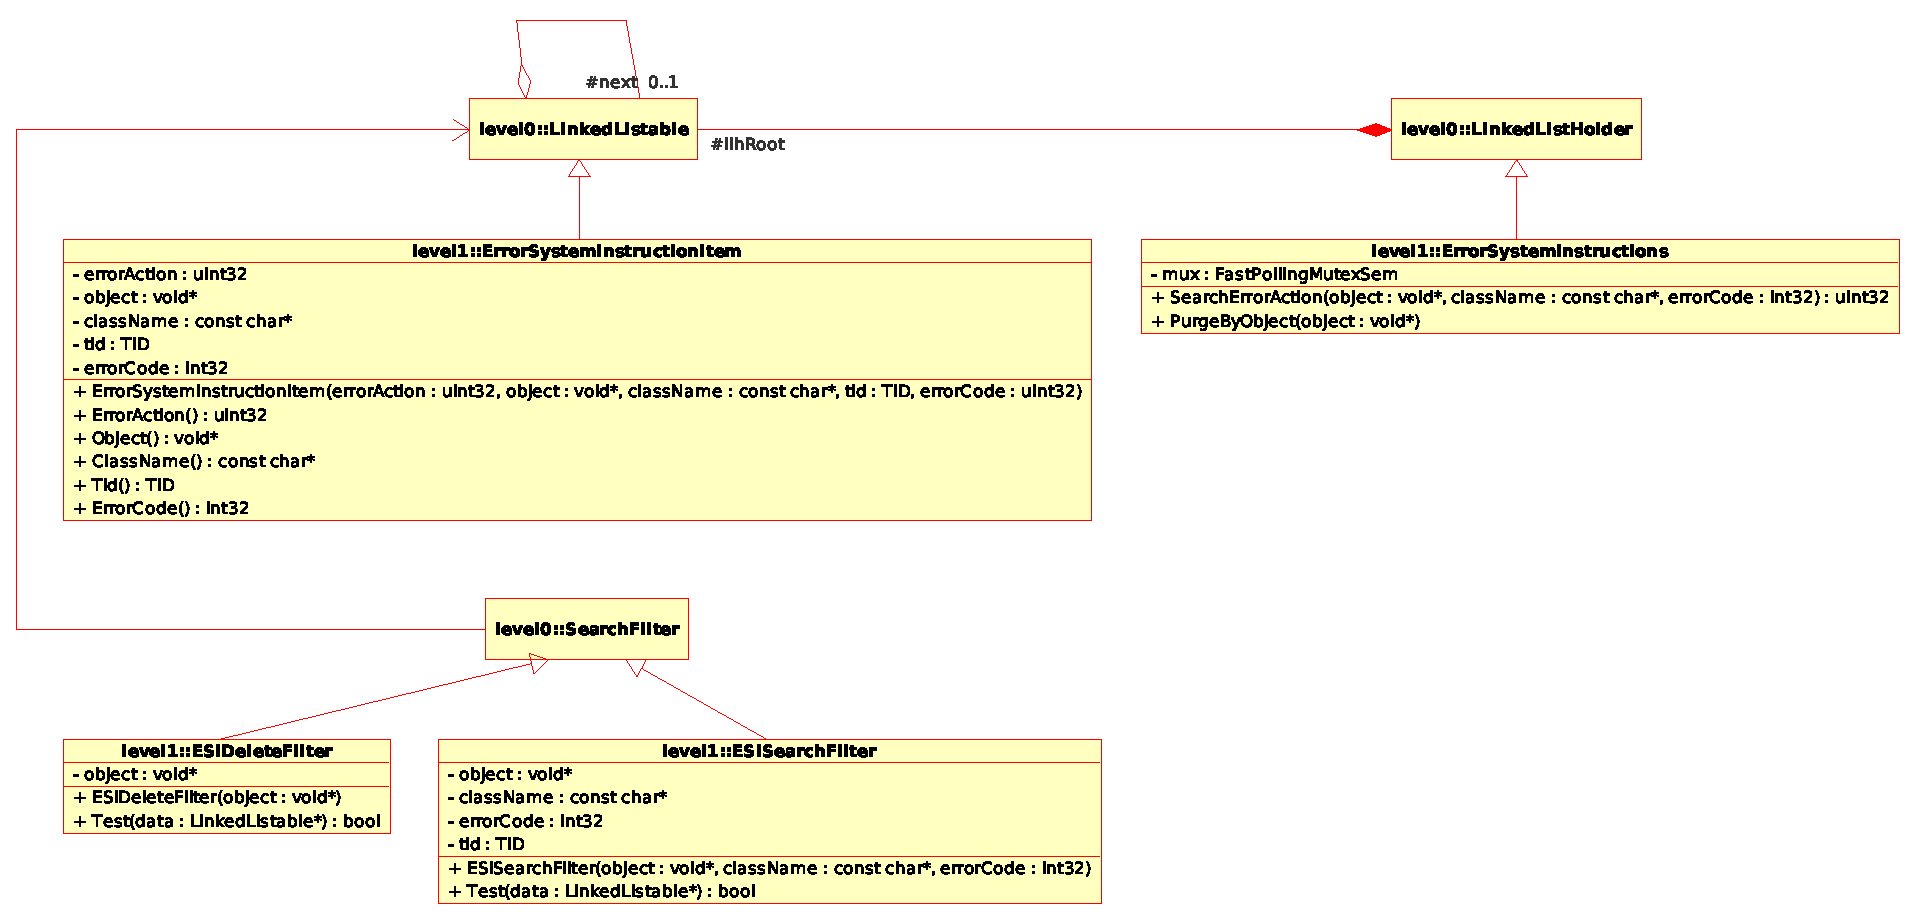
\includegraphics[width=\textwidth]{level1/level1-ESI.eps}
  \caption{BaseLib Level1 Error System Instruction classes}
  \label{f:level1:esi}
 \end{center}
\end{figure}

The UML diagram is depicted in Figure \ref{f:level1:esi} but if you look also to Figure \ref{f:level1:object} you can note that also \texttt{Object} relies on top of the ESI infrastructure; for each class type there is also an ESI item that decides what action to take in case of an error condition.\\

ESI is another linked listable structure that accounts about errors, i.e. is a catalog of errors and actions, classes involved in this level are:

\begin{itemize}
 \item ErrorSystemInstructionItem
 \item ErrorSystemInstructions
 \item ESIDeleteFilter, ESISearchFilter
\end{itemize}



\subsubsection{ErrorSystemInstructionItem}
\texttt{[ErrorSystemInstructionItem.h]}\\
The basic component of the ESI is the class \texttt{ErrorSystemInstructionItem}, there is a class like that for every error and basically tall the system what to do in case a specific error.

We start with the attributes, the first attribute, \texttt{errorAction}, tell the system what to do with this error, \texttt{object} is the address of the object the action is restricted to, attribute \texttt{className} is the name of class the action is restricted to, \texttt{tid} is the thread identification the action is restricted to and \texttt{errorCode} is the error code the action is restricted to. If you choose to not restrict error management to any of the previous attributes simply sets them to \texttt{NULL}.

The constructor lets you set the policy for an error, all the other methods let you get the attributes of the class.
\begin{lstlisting}[
extendedchars=true,%
basicstyle=\fontfamily{pcr}\fontseries{m}\selectfont\footnotesize, %
stepnumber=1,%
numberstyle=\tiny,%
keywordstyle=\footnotesize\tt ,%
language=C++]
   uint32 errorAction;
   void* object;
   const char* className;
   TID tid;
   int32 errorCode;
public:
   ErrorSystemInstructionItem(uint32 errorAction,
         void* object,
         const char* className,
         TID tid,
         int32 errorCode);
   uint32 ErrorAction();
   void* Object();
   const char* ClassName();
   TID Tid();
   int32 ErrorCode();
\end{lstlisting}

Some defined \texttt{ErrorSystemInstructionItem} in file \textit{level1/ErrorSystemInstructionItem.h}:
\begin{lstlisting}[
extendedchars=true,%
basicstyle=\fontfamily{pcr}\fontseries{m}\selectfont\footnotesize, %
stepnumber=1,%
numberstyle=\tiny,%
keywordstyle=\footnotesize\tt ,%
language=C++]
#define ANY_VALUE NULL

#define OBJECT_ERRORINSTRUCTION(errorAction,object,code) \
   new ErrorSystemInstructionItem(errorAction,object,ANY_VALUE,ANY_VALUE,code)
#define ERRCODE_ERRORINSTRUCTION(errorAction,code) \
   new ErrorSystemInstructionItem(errorAction,ANY_VALUE,ANY_VALUE,ANY_VALUE,code)
#define CLASS_ERRORINSTRUCTION(errorAction,classInfo,code) \
   new ErrorSystemInstructionItem(errorAction,ANY_VALUE,classInfo,ANY_VALUE,code)
#define TID_ERRORINSTRUCTION(errorAction,tid,code) \
   new ErrorSystemInstructionItem(errorAction,ANY_VALUE,ANY_VALUE,tid,code)
\end{lstlisting}



\subsubsection{ErrorSystemInstructions}
\texttt{[ErrorSystemInstructions.h]}\\
The class \texttt{ErrorSystemInstructions} is a collection of \texttt{ErrorSystemInstructionItem}s, i.e. a container of \texttt{ErrorSystemInstructionItem}: what to do in case of an error. It is a subclass of \texttt{LinkedListHolder}.

The only added attribute to the \texttt{LinkedListHolder} class is a \texttt{FastPollingMutexSem} that manages the access to the resources. The method \texttt{SearchErrorAction} searches using one of the three keys as arguments an method \texttt{PurgeByObject} remove the \texttt{ErrorSystemInstructionItem} associated to an object passed by pointer.
\begin{lstlisting}[
extendedchars=true,%
basicstyle=\fontfamily{pcr}\fontseries{m}\selectfont\footnotesize, %
stepnumber=1,%
numberstyle=\tiny,%
keywordstyle=\footnotesize\tt ,%
language=C++]
   FastPollingMutexSem mux;
public:
   uint32 SearchErrorAction(void *object,const char *className,int32 errorCode);
   void PurgeByObject(void *object);
\end{lstlisting}



\subsubsection{ESIDeleteFilter, ESISearchFilter}
\texttt{[ErrorSystemInstructions.h]}\\
Methods implemented in the previous \texttt{ErrorSystemInstructions} class work using the class defined in this section: \texttt{ESIDeleteFiler} and \texttt{ESISearchFilter}. The first one, \texttt{ESIDeleteFilter}, is a filter to delete \texttt{ErrorSystemInstructionItem}; and the last one, \texttt{ESISearchFilter}, searches for \texttt{ErrorSystemInstructionItem} by different criteria.



\section{Configuration Database}
The \textit{Configuration Database} (CDB) is one of the key concepts upon BaseLib is developed. There are not to many classes in this level concerning the CDB, infact its classes are spreaded across many levels. In this level the developer will find a sort of interface to CDB: the \texttt{CDBVirtual} abstract class that by the way can be considered as an interface but has one non pure virtual method.

In next levels we will face with three CDBs' implementations (CDB, CDBOS, MMCDB). If one want to go a bit further can write a CDB that parse XML file for example and make it work in the framework simply let it work observe the interface we are now discussing about in this section.

\begin{figure}[h!]
 \begin{center}
  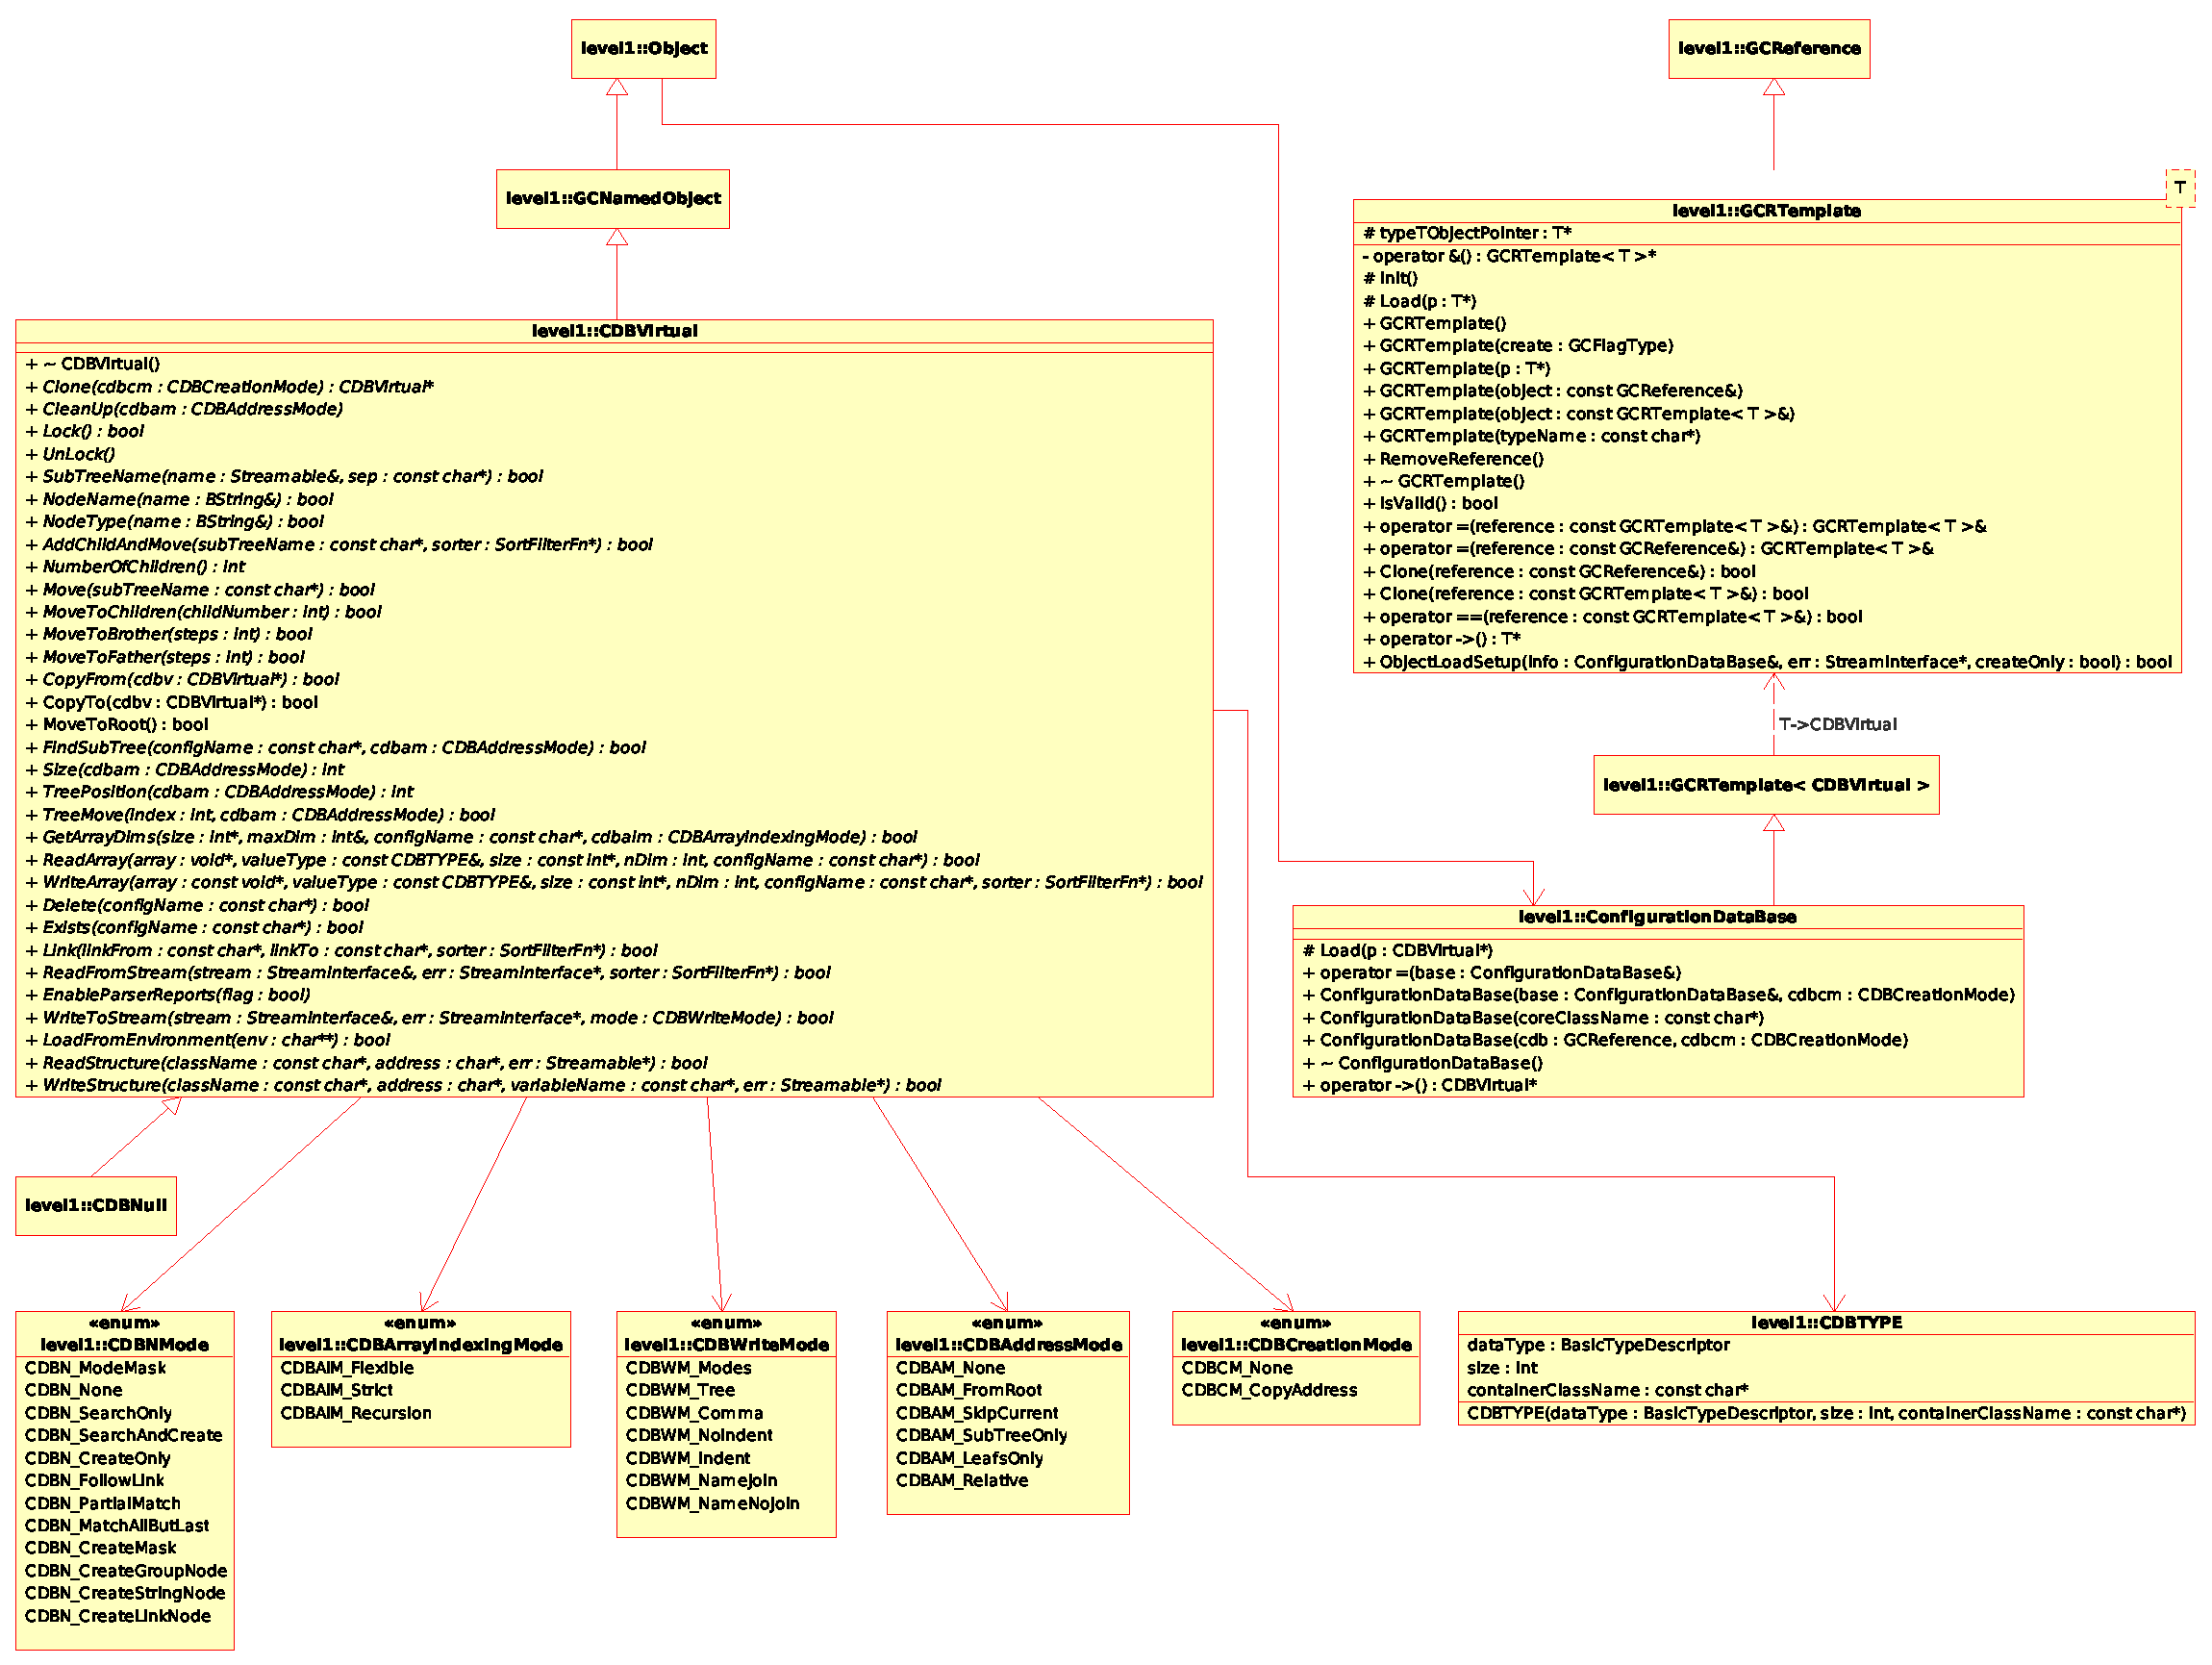
\includegraphics[width=\textwidth]{level1/level1-CDB.eps}
  \caption{BaseLib Level1 Configuration Database classes}
  \label{f:level1:CDB}
 \end{center}
\end{figure}

Figure \ref{f:level1:CDB} depicts the UML diagram of the involved classes that are:
\begin{itemize}
 \item CDBVirtual
 \item CDBNull
 \item ConfigurationDataBase
\end{itemize}



\subsubsection{CDBVirtual}
\texttt{[CDBVirtual.h, CDBTypes.h]}\\
The class \texttt{CDBVirtual} provide an interface to a hierarchical database. It works similarly to a filesystem having directory nodes (branches) and file nodes (leaves). Each leaf node is a container of a sequence of characters, both ASCII and not ascii. CDB is infact a reference to an instance of the database. Copying CDBs does not duplicate the database but increases a reference counter. Operation to the same database by different threads is safe. The methods of this class are not usable directly outside BaseLib Use \texttt{CreateCDB} to create an instance of CDB. \\


Class \texttt{CDBVirtual} has many pure virtual methods, we go throught those. In the file \textit{level1/CDBTypes.h} all the enumeration used are can be founded.

The deconstructor will destroy database if instance count goes to zero. The method \texttt{Clone} creates a new reference to a database, or if that is not possible it creates a copy; \texttt{cdbcm=CDBCM\_CopyAddress} ensures that the new object points at the same location. The method \texttt{CleanUp} removes all the content from the database unless some other database instance exists and points to a subtree, one can reques to delete only the current subtree.
The method \texttt{Lock} locks the main database for exclusive access: use if a group of transactions should be atomic; \texttt{UnLock} unlocks the main database: remember to unlocking a locked database after useing it.
\begin{lstlisting}[
extendedchars=true,%
basicstyle=\fontfamily{pcr}\fontseries{m}\selectfont\footnotesize, %
stepnumber=1,%
numberstyle=\tiny,%
keywordstyle=\footnotesize\tt ,%
language=C++]
   virtual ~CDBVirtual();
   virtual CDBVirtual* Clone(CDBCreationMode cdbcm)=0;
   virtual void CleanUp(CDBAddressMode cdbam=CDBAM_FromRoot) = 0;
   virtual bool Lock() = 0;
   virtual void UnLock() = 0;
\end{lstlisting}

The method \texttt{SubTreeName} finds the overall path leading to the current node, return the path in the argument \texttt{name}, \texttt{NodeName} returns the name of the current node in \texttt{name}; \texttt{NodeType} return the type of the current node in \texttt{name}; the method \texttt{AddChildAndMove} can be used to create a new subtree.

The method \texttt{NumberOfChildren} tells how many branches from this node, negative number implies that the location is a leaf; \texttt{Move} moves to the specified location; the movement is relative to the current location, \texttt{UpNode} is one level up, \texttt{RootNode} is all the way up. The mehtod \texttt{MoveToChildren} lets you move in the tree, negative numbers move up, 0 is the first of the children and a positive number is the n-th children; \texttt{MoveToFather} let s you move in the tree, 0 means remain where you are, greater then 0 to brothers on the right below 0 on the left. The method \texttt{CopyFrom} and \texttt{CopyTo} copy from the CDB to another one. \texttt{MoveToRoot} moves back to the root of the tree.
The method \texttt{FindSubTree} searches on the right of the tree for the subtree identified by the string \texttt{configName}; on success nodes points to the node containing the subtree or leaf; it will not follow links; the only argument it supports is \texttt{CDBAM\_SkipCurrent} that allow a search in the current subtree excluding current node any other flag are NOT SUPPORTED.
The method \texttt{Size} gives the total number of nodes; argument can be \texttt{CDBAM\_SubTreeOnly} allowing to measure the current subtree, or \texttt{CDBAM\_LeafsOnly}   allowing counting only the data nodes. \texttt{TreePosition} returns the position of the node in the left to right bottom to top order the absolute location of a node; \texttt{CDBAM\_LeafsOnly} allows counting only the data nodes. The method \texttt{TreeMove} moves to a location within the whole (sub)tree; the nodes are numbered from left to right and from subnode to supernode; if the node does not exist returns False and remains in the start position.

\begin{lstlisting}[
extendedchars=true,%
basicstyle=\fontfamily{pcr}\fontseries{m}\selectfont\footnotesize, %
stepnumber=1,%
numberstyle=\tiny,%
keywordstyle=\footnotesize\tt ,%
language=C++]
   virtual bool SubTreeName(Streamable& name,const char* sep = ".") = 0;
   virtual bool NodeName(BString& name) = 0;
   virtual bool NodeType(BString& name) = 0;

   virtual bool AddChildAndMove(const char* subTreeName,
      SortFilterFn* sorter=NULL) = 0;
   virtual int  NumberOfChildren()=0;
   virtual bool Move(const char* subTreeName) = 0;
   virtual bool MoveToChildren(int childNumber=0) = 0;
   virtual bool MoveToBrother(int steps = 1) = 0;
   virtual bool MoveToFather(int steps = 1) = 0;
   virtual bool CopyFrom(CDBVirtual* cdbv) = 0;
   inline bool  CopyTo(CDBVirtual* cdbv);
   inline  bool MoveToRoot();

   virtual bool FindSubTree(const char* configName,
      CDBAddressMode cdbam=CDBAM_None)=0;
   virtual int  Size(CDBAddressMode cdbam) = 0;
   virtual int  TreePosition(CDBAddressMode cdbam=CDBAM_LeafsOnly) = 0;
   virtual bool TreeMove(int index,
      CDBAddressMode cdbam=CDBAM_LeafsOnly) = 0;
\end{lstlisting}

The method \texttt{GetArrayDims} if doesn't fail returns the \texttt{size}, \texttt{maxDim} and \texttt{configName} of the CDB. The method \texttt{ReadArray} read the array, if \texttt{size} is \texttt{NULL} it treats the input as a monodimensional array of size \texttt{nDim}, if \texttt{nDim} is zero this is a standard variable equivalent of a vector of size 1, if size does not agree with the actual dimensions of the matrix the routine will fail. We can tell the same for the \texttt{WriteArray} method.\\


The method \texttt{Delete} removes an entry or subtree (position is relative) to delete a link use the \texttt{linkTo} as the leaf name to delete a subtree simply specify the group node. The method \texttt{Exists} tell you whether a certain entry exists. The method \texttt{Link} make a link, \texttt{linkFrom} is the path where the link is created from.\\


The method \texttt{ReadFromStream} reads a database from a stream; \texttt{EnableParserReports} enables reports of parser during \texttt{ReadFromStream} into error stream. \texttt{WriteToStream} writes the database to stream without any ordering; \texttt{LoadFromEnvironment} loads from environment or from any \texttt{NULL} terminated list of chars.\\


The method \texttt{ReadStructure} read from CDB to memory and the method \texttt{WriteStructure} either copies or references a memory structure, at address \texttt{address} and of type \texttt{className} CDB transforms the memory.

\begin{lstlisting}[
extendedchars=true,%
basicstyle=\fontfamily{pcr}\fontseries{m}\selectfont\footnotesize, %
stepnumber=1,%
numberstyle=\tiny,%
keywordstyle=\footnotesize\tt ,%
language=C++]
   virtual bool GetArrayDims(int* size, int& maxDim, const char* configName,
      CDBArrayIndexingMode cdbaim=CDBAIM_Flexible) = 0;
   virtual bool ReadArray(void* array, const CDBTYPE& valueType,
      const int* size, int nDim, const char* configName) = 0;
   virtual bool WriteArray(const void* array, const CDBTYPE& valueType,
      const int* size, int nDim, const char* configName, 
      SortFilterFn* sorter=NULL) = 0;

   virtual bool Delete(const char* configName) = 0;
   virtual bool Exists(const char* configName) = 0;
   virtual bool Link(const char* linkFrom,
      const char* linkTo,
      SortFilterFn* sorter=NULL) = 0;

   virtual bool ReadFromStream(StreamInterface& stream,
      StreamInterface* err=NULL,SortFilterFn* sorter=NULL) = 0;
   virtual void EnableParserReports(bool flag) = 0;
   virtual bool WriteToStream(StreamInterface& stream,
      StreamInterface* err=NULL,CDBWriteMode mode=CDBWM_Tree) = 0;
   virtual bool LoadFromEnvironment(char** env) = 0;

   virtual bool ReadStructure (const char* className,
      char* address,
      Streamable* err=NULL) = 0;
   virtual bool WriteStructure(const char* className,
      char* address,
      const char* variableName=NULL,
      Streamable* err=NULL) = 0;
\end{lstlisting}



\subsubsection{CDBNull}
\texttt{[CDBNull.h]}\\
Class \texttt{CDBNull} is a dummy CDB just to create valid references. Each method is implemented returning zero or \texttt{False}.



\subsubsection{ConfigurationDataBase}
\texttt{[ConfiguratonDataBase.h]}\\
Differently from other data structures that we have founded during this chapter, like ORDB and GODB, you can instantiate how many \textit{Configuration Database}s you need and there is no static and globally defined CDB. A \texttt{ConfigurationDataBase} contains a reference to CDB of type \texttt{CDBVirtual} because it inherits from \texttt{GCRTemplate<CDBVirtual>}. Forces call to CDB to be made via the virtual table. \\


The method \texttt{Load} copy the \texttt{CDBVirtual} pointer in the \texttt{GCRTemplate} templatized attribute \texttt{typeTObjectPointer} after type checking. The first constructor
 creates a new database if \texttt{base} paramenter is \texttt{NULL}, if not \texttt{NULL} it creates a reference to an existing one. The second constructor creates a CDB from a generic base type.

\begin{lstlisting}[
extendedchars=true,%
basicstyle=\fontfamily{pcr}\fontseries{m}\selectfont\footnotesize, %
stepnumber=1,%
numberstyle=\tiny,%
keywordstyle=\footnotesize\tt ,%
language=C++]
protected:
   void Load(CDBVirtual *p);
public:
   inline ConfigurationDataBase(ConfigurationDataBase &base,
      CDBCreationMode cdbcm=CDBCM_CopyAddress);
   inline ConfigurationDataBase(const char* coreClassName="CDB");
   inline ConfigurationDataBase(GCReference cdb,
      CDBCreationMode cdbcm=CDBCM_CopyAddress);
   inline void operator=(ConfigurationDataBase &base);

   virtual  ~ConfigurationDataBase();
   CDBVirtual *operator->();
\end{lstlisting}



\subsection{Design Notes}
The class \texttt{ConfigurationDataBase} declared with all inline methods in \textit{level1/ConfigurationDataBase.h} is included in many BaseLib's files, this way the code will be compiled to many times wasting space. Class \texttt{CDBVirtual} looks so heavy could be stripped off?

\chapter{BaseLib Level 2}
\chaptermark{Level 2}

%andre articolo
A series of classes are dedicated to strings and data streaming. These allow to perform a series of advanced operations in character sequences and to perform input/output (I/O) operations without requiring the concept of beginning and end of transmission. Most of the I/O classes are abstracted to a level where the knowledge of the target media (socket, memory, ...) isn't required. Such classes come from BaseLib Level 2 and inherits from \texttt{level0::StreamInterface} and its implementation \texttt{level2::Streamable}.\\


The main concept in this chapter is the \texttt{Streamable} class that is presented before every other class.
As usual we discuss each section in a logical order; Level2 asa said before implements the concept of stream, a common concept in C++ and in Java, slighty new to C programmers that are used to work with files, sockets or strings. All this concepts are groupped togheter and are accesible via the \texttt{level0::StreamInterface}. \texttt{Streamable} implements \texttt{StreamInterface} and adds some metods and attributes.\\


Analysis is carried on examining the differents stream object grouped in two sets: memory (buffer, string handling) and files (also sockets that are no more than files in Unix view). The whole BaseLib Level 2 could be divided in the following sections:
\begin{itemize}
 \item Streamable (memory, files)
 \item CDB
 \item IO devices (serial line, keyboard)
\end{itemize}



\section{Streamable}
Before reading this section is really important that one has read \textit{BaseLib} \textit{Level0} \textit{Streams} section. Such a section introduces streams and the \texttt{StreamInterface} from which the \texttt{Streamable} inherits from. This section treats first the class \texttt{Streamable} and then we have a look first to memory streams and then to file streams. We take a look first to memory streams because there is an important class on which the \texttt{Streamable} class relies on. To have a pictorial idea of the \texttt{Streamable} class introduced below refer to Figure \ref{f:level2:stream_mem} and Figure \ref{f:level2:stream_file}.



\subsubsection{Streamable}
\texttt{[Streamable.h, Streamable.cpp]}\\
Most of the methods in \texttt{Streamable} class are an implementation of what is simply declared in the \texttt{StreamInterface} class in Level0. \texttt{Streamable} is the prototype for all streams, it adds to StreamInterface some buffering and token searching functions.\\


The class \texttt{Streamable} relies on the \texttt{CStreamBuffering} class described in the following sections, of such type are the first two attributes, the first is the \textit{input} buffering area and the second is the \textit{output} buffering area (\texttt{csbIn} and \texttt{csbOut}). Last attribute is a stream identifier, if hold the value \texttt{0} means the default stream and if is \texttt{-1} it means no stream.

The constructor simply set to \texttt{NULL} each attribute and the destructor does nothing.
\begin{lstlisting}[
extendedchars=true,%
basicstyle=\fontfamily{pcr}\fontseries{m}\selectfont\footnotesize, %
stepnumber=1,%
numberstyle=\tiny,%
keywordstyle=\footnotesize\tt ,%
language=C++]
protected:
   CStreamBuffering* csbIn;
   CStreamBuffering* csbOut;
   uint32 selectedStream;
public:
   Streamable();
   virtual ~Streamable();
\end{lstlisting}

The first two methods we encounter, \texttt{SSRead} and \texttt{SSWrite} are two virtual methods not implemented here but to be implemented by any subclass. \texttt{CanRead} and \texttt{CanWrite} simply return \texttt{False} because methods \texttt{SSRead}, \texttt{SSWrite} are not implemented for the class. Methods \texttt{Read} and \texttt{GetC} call \texttt{SSRead}; methods \texttt{Write} and \texttt{PutC} call \texttt{SSWrite}.
\begin{lstlisting}[
extendedchars=true,%
basicstyle=\fontfamily{pcr}\fontseries{m}\selectfont\footnotesize, %
stepnumber=1,%
numberstyle=\tiny,%
keywordstyle=\footnotesize\tt ,%
language=C++]
protected:
   virtual bool SSRead(void* buffer,uint32& size,TimeoutType msecTimeout=TTDefault)=0;
   virtual bool SSWrite(const void* buffer,uint32& size,TimeoutType msecTimeout=TTDefault)=0;

public:
   virtual bool Read(void* buffer,uint32& size,TimeoutType msecTimeout=TTDefault);
   virtual bool Write(const void* buffer,uint32& size,TimeoutType msecTimeout=TTDefault);

   virtual bool CanRead();
   virtual bool CanWrite();

   inline bool GetC(char& c);
   inline bool PutC(char c);
\end{lstlisting}

The method \texttt{Size} must return the size of the file, in this case it will return\texttt{-1} because \texttt{Streamable} is an abstract class; the same happens for the method \texttt{Position}. Methods \texttt{SetSize}, \texttt{Seek} and \texttt{CanSeek} return \texttt{False}. All those methods must be implemented in a subclass. \\


The method \texttt{NOfStreams} return \texttt{1}, such method return how many streams are available, override it with a different value if multiple stream are supported. The first \texttt{Switch} method select the stream to read from, switching may reset the stream to the start, \texttt{0} is the default stream, \texttt{false} is only returned if the switch was not performed. Also the second \texttt{Switch} selects the stream to read from, must be overriden with a method providing name to number mapping. The method \texttt{SelectedStream} returns what stream has been selected and \texttt{StreamName} returns the name of the stream we are using.
The method \texttt{AddStream} adds a new stream to write in and \texttt{RemoveStream} removes an existing stream. Those last two methods are not implemented in this class and return \texttt{false}.\\


The method \texttt{CompleteRead} performs the job of a the read function but guarantees the completion; in case of failure, \texttt{size} returns the actual data read; \texttt{timeOutMs} is the total allowed wait time checked using \texttt{level0::HRT}. The method \texttt{CompleteWrite} performs the job of a write function but guarantees the completion; in case of failure size returns the actual data written; those functions are implemented in the \textit{Streamable.cpp} file.
\begin{lstlisting}[
extendedchars=true,%
basicstyle=\fontfamily{pcr}\fontseries{m}\selectfont\footnotesize, %
stepnumber=1,%
numberstyle=\tiny,%
keywordstyle=\footnotesize\tt ,%
language=C++]
   virtual int64 Size();
   virtual bool SetSize(int64 size);
   virtual int64 Position(void);
   virtual bool Seek(int64 pos);
   virtual bool CanSeek();

   virtual uint32 NOfStreams();
   virtual bool Switch(uint32 selectedStream);
   virtual bool Switch(const char* name);
   virtual uint32 SelectedStream();
   virtual bool StreamName(uint32 n,char* name,int nameSize);
   virtual bool AddStream(const char* name);
   virtual bool RemoveStream(const char *name);

   virtual bool CompleteRead(void* buffer,uint32& size,
      TimeoutType msecTimeout = TTInfiniteWait);
   virtual bool CompleteWrite(const void* buffer,uint32& size,
      TimeoutType msecTimeout = TTInfiniteWait);
\end{lstlisting}

Now we introduce three functions firstly implemented in the \texttt{Streamable} class, those function make use of the attributes in the \texttt{Streamable} class.

The method \texttt{BufferedRead} writes the buffer from the stream; it's better to not remap this function unless the class needs to deal with buffering in a different way.
The method \texttt{BufferedWrite} reads and copies data into the stream; it is important to not remap this function unless the class needs to deal with buffering in a different way, like the previous method. \texttt{Flush} forces to complete buffered operations.
\begin{lstlisting}[
extendedchars=true,%
basicstyle=\fontfamily{pcr}\fontseries{m}\selectfont\footnotesize, %
stepnumber=1,%
numberstyle=\tiny,%
keywordstyle=\footnotesize\tt ,%
language=C++]
   virtual bool BufferedRead(void* buffer,uint32& size,
      TimeoutType msecTimeout = TTDefault);
   virtual bool BufferedWrite(const void* buffer,uint32& size,
      TimeoutType msecTimeout = TTDefault);
   inline void Flush();
\end{lstlisting}

The method \texttt{VPrintf} will write any text using printf format (is buffered if buffering is activated), the others \texttt{Print} functions print, respectively, an integer, a flot or a string with desidered size and padding to the output stream registered with the \texttt{Streamable} class (attribute \texttt{csbOut}).
\begin{lstlisting}[
extendedchars=true,%
basicstyle=\fontfamily{pcr}\fontseries{m}\selectfont\footnotesize, %
stepnumber=1,%
numberstyle=\tiny,%
keywordstyle=\footnotesize\tt ,%
language=C++]
   bool VPrintf(const char* format,va_list argList);
   inline bool Print(int32 n,int desiredSize=0,
      char desiredPadding=0,char mode = 'i');
   inline bool Print(double f,int desiredSize=0,
      int desiredSubSize=6,char desiredPadding=0,char mode='f');
   inline bool Print(const char* s,int desiredSize=0,
      char desiredPadding=0);
\end{lstlisting}


First \texttt{GetToken} method extracts a token from the stream into a string data until a terminator or 0 is found; \texttt{maxSize} is the buffer size, the maximum string size is \texttt{maxSize-1}; it skips all \texttt{skipCharacters} chars even if calssified also as terminators if at the beginning returns \texttt{true} if some data was read before any error or file termination. \texttt{false} only on error and no data available; the terminator (just the first encountered) is consumed in the process and saved in \texttt{saveTerminator} if provided. This is a buffered method.
Second \texttt{GetToken} method behave in the same way as before but takes as the first argument an \texttt{StreamInterface} object. A character can be found in the terminator or in the \texttt{skipCharacters} list in both or in none. See Table \ref{t:level2:gettoken} for an explanation on how it work. The same things can be said for the third \texttt{GetToken} but it takes a string as a \texttt{Streamable} reference.

\begin{table}[!h]
 \begin{center}
  \begin{tabular}{|l|l|}
   \hline
    \textbf{char in} & \textbf{action preformed} \\
   \hline
    none & the character is copied \\
    terminator & the character is not copied the string is terminated \\
    skip & the character is not copied \\
    skip and terminator & the character is not copied, the string is terminated if not empty \\
   \hline
   \end{tabular}
   \end{center}
  \caption{Level2 GetToken actions}
 \label{t:level2:gettoken}
\end{table}

\texttt{SkipTokens} skips a series of tokens delimited by terminators or 0.
\texttt{GetLine} will skip an empty line or any part of a line termination (the first working on a \texttt{Streamable} input and the second on a \texttt{char*} input extracting the substring after skipping the required line). \\


Next two methods are \texttt{static}, the first one \texttt{GetCStringToken} extracts a token from the string into a string until a terminator or 0 is found, the maximum string size is $maxSize-1$, it returns \texttt{true} if some data was read. False only on no data available. The method \texttt{DestructiveGetCStringToken} extracts a token from the string into a string until a terminator or 0 is found and affects the input by placing 0 at the end of each token.\\


Last method, \texttt{FindPattern} extracts data from the stream until the matching string is found the pointer is to the first character after the pattern.
\begin{lstlisting}[
extendedchars=true,%
basicstyle=\fontfamily{pcr}\fontseries{m}\selectfont\footnotesize, %
stepnumber=1,%
numberstyle=\tiny,%
keywordstyle=\footnotesize\tt ,%
language=C++]
   virtual bool GetToken(char* buffer,const char* terminator,
      uint32 maxSize,char* saveTerminator=NULL,const char* skipCharacters=NULL);
   virtual bool GetToken(StreamInterface& output,const char* terminator,
      char* saveTerminator=NULL,const char* skipCharacters=NULL);
   virtual bool GetToken(Streamable& output,const char* terminator,
      char* saveTerminator=NULL,const char* skipCharacters=NULL);

   virtual bool SkipTokens(uint32 count, const char* terminator);
   virtual bool GetLine(Streamable& output, bool skipTerminators=True);
   virtual bool GetLine(char* buffer,uint32 maxSize,bool skipTerminators=True);

   static inline bool GetCStringToken(const char*& input,char* buffer,
      const char* terminator,uint32 maxSize);
   static inline char* DestructiveGetCStringToken(char*& input,const char* terminator,
      char* saveTerminator=NULL,const char* skipCharacters="");

   inline bool FindPattern(const char *pattern);
\end{lstlisting}



\subsection{Memory Streams}
Memory streams are all streams involving memory operations like strings and buffers. All classes that depend on this group are depicted in the UML diagram of Figure \ref{f:level2:stream_mem}.
\begin{figure}[h!]
 \begin{center}
  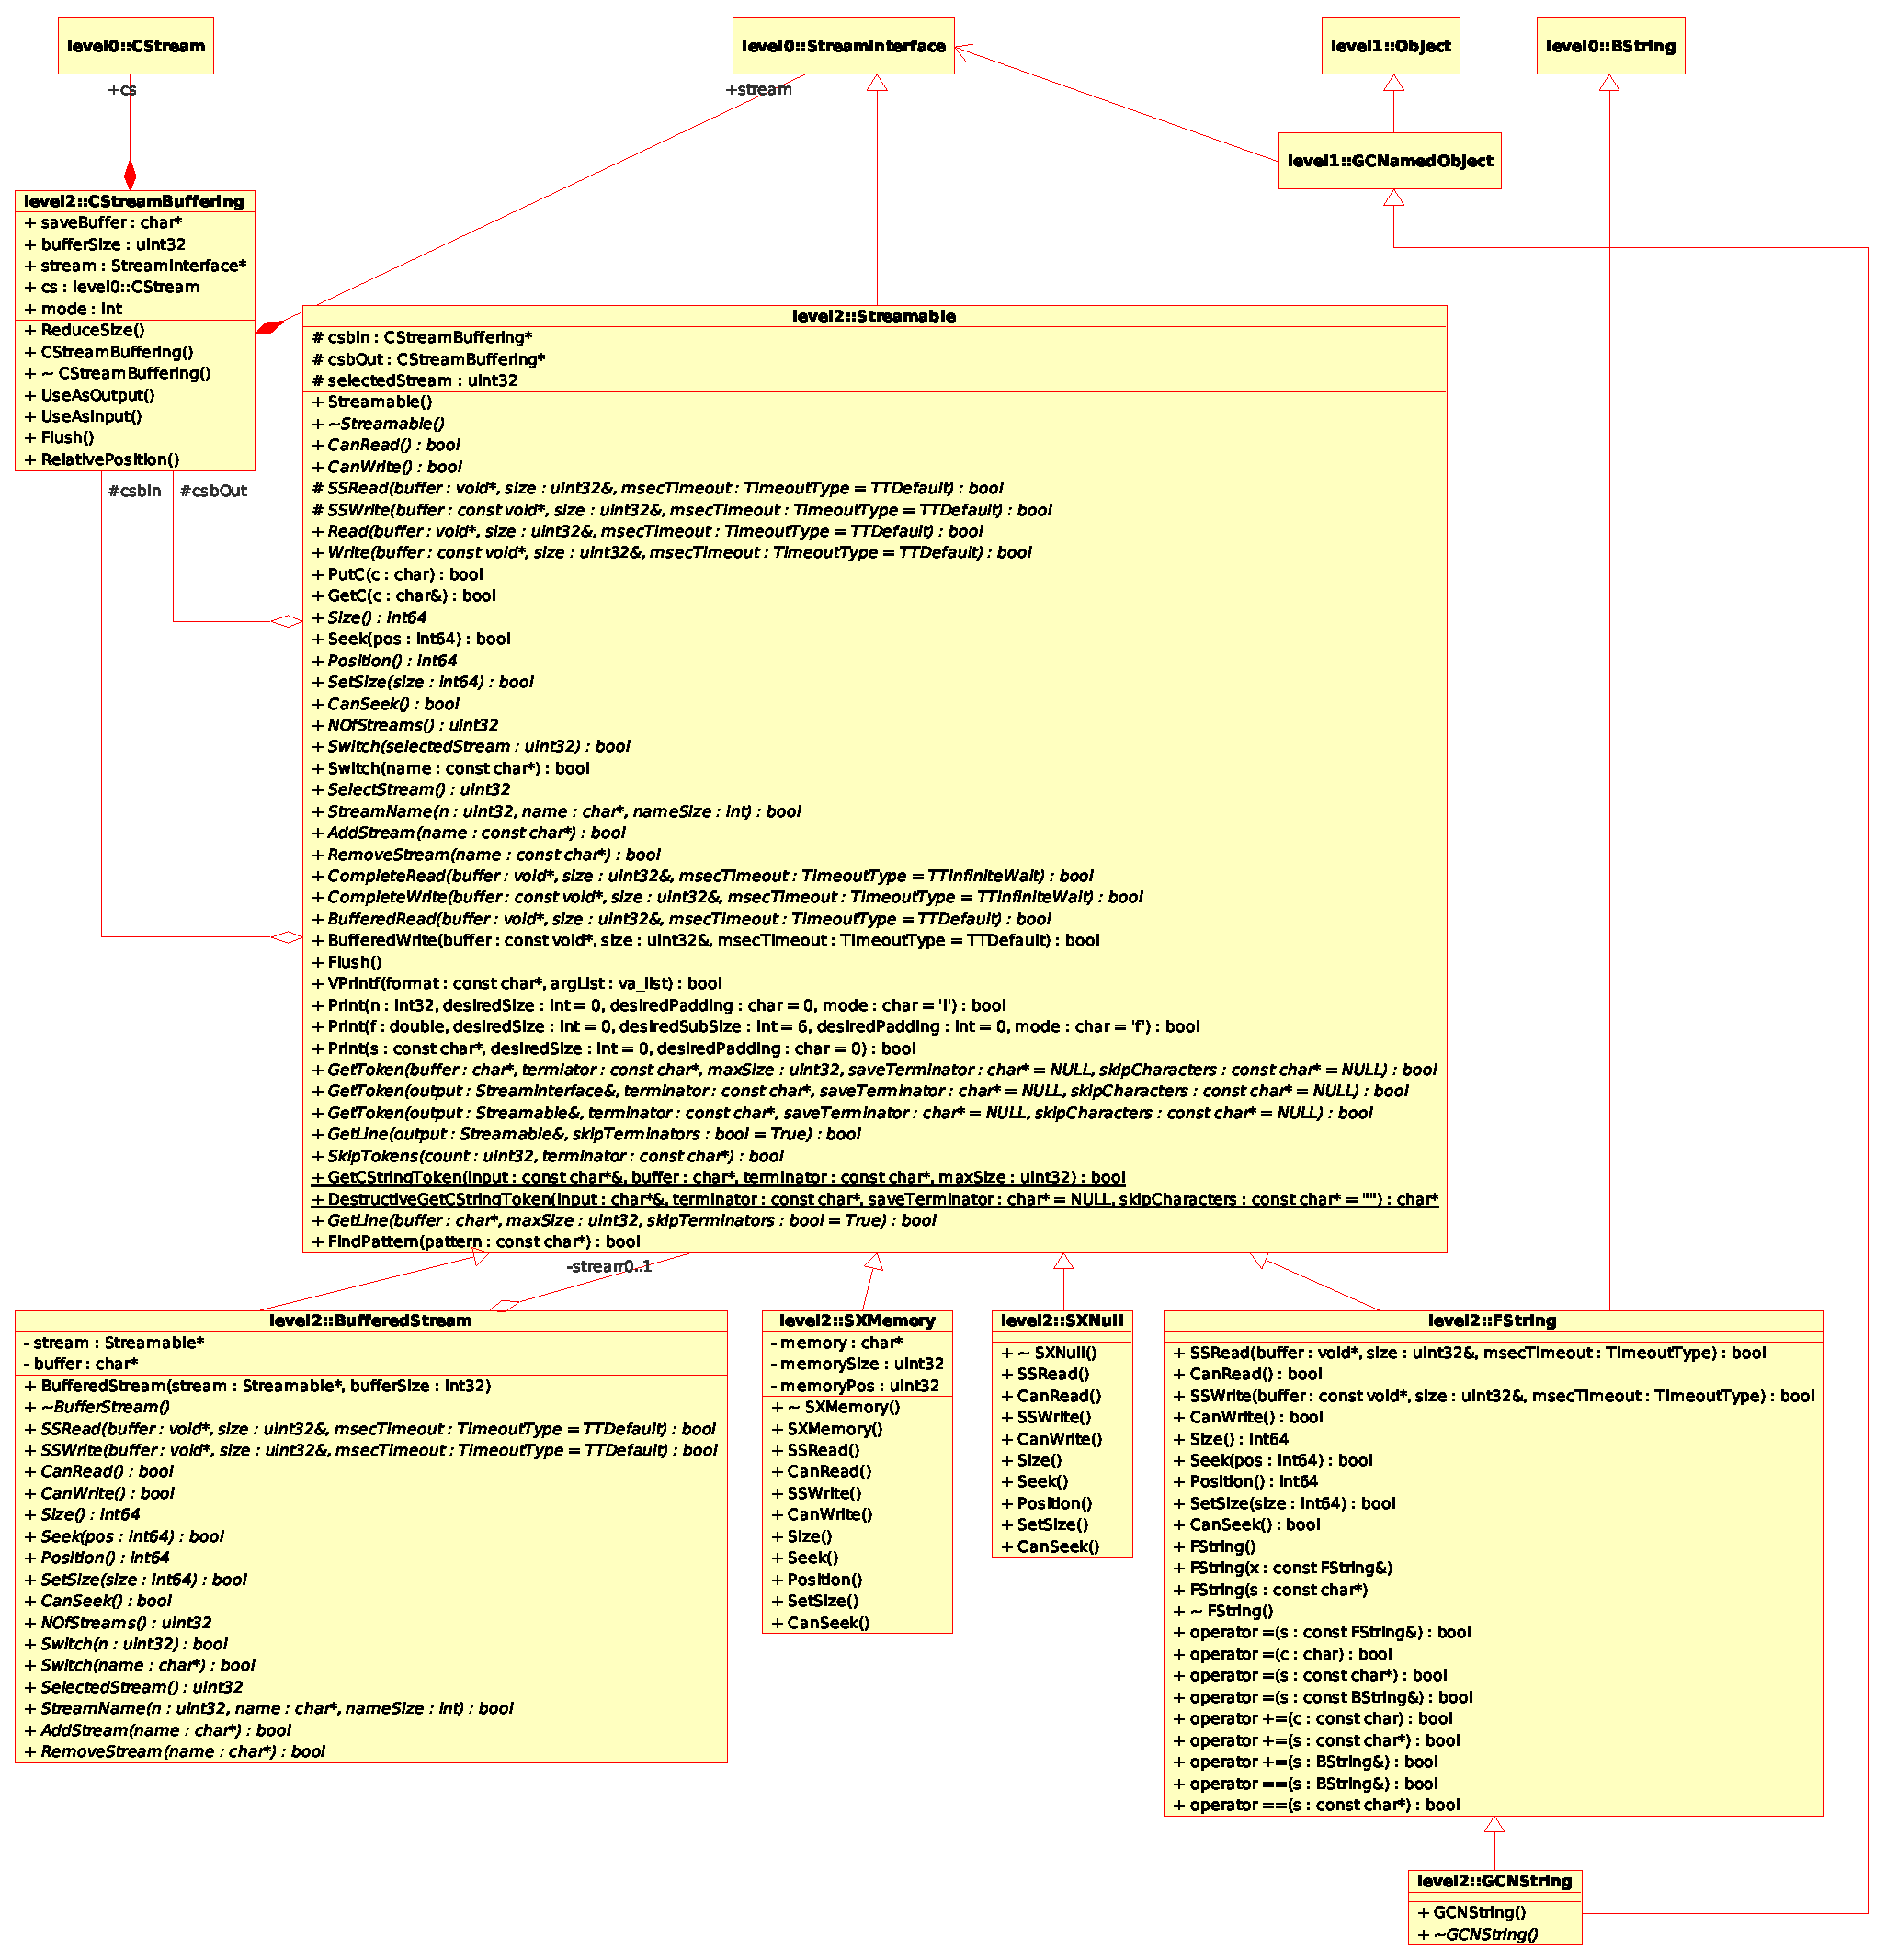
\includegraphics[width=\textwidth]{level2/level2-mstream.eps}
  \caption{BaseLib Level2 memory stream classes}
  \label{f:level2:stream_mem}
 \end{center}
\end{figure}

Class involved are listed below. Most of the classes are quite similar, the only notable difference is the \texttt{CStreamBuffering} class that is not a subclass of the \texttt{Streamable} class. We start analysing this class.
\begin{itemize}
 \item CStreamBuffering
 \item BufferedStream
 \item SXMemory, SXNull
 \item FString, GCNString
\end{itemize}



\subsubsection{CStreamBuffering}
\texttt{[CStreamBuffering.h, CStreamBuffering.cpp]}\\
This class basically maps a \texttt{StreamInterface} to a \texttt{CStream} class providing buffering to the \texttt{CStream}.

The class has infact as attributes a \texttt{StreamInterface} pointer and a \texttt{CStream}. The constructor let the user set those attributes. The working mode, attribute \texttt{mode}, can be set with \texttt{UseAsOutput} and \texttt{UseAsInput}.
\begin{lstlisting}[
extendedchars=true,%
basicstyle=\fontfamily{pcr}\fontseries{m}\selectfont\footnotesize, %
stepnumber=1,%
numberstyle=\tiny,%
keywordstyle=\footnotesize\tt ,%
language=C++]
public:
   char* saveBuffer;
   uint32 bufferSize;
   StreamInterface* stream;
   CStream cs;
   int mode;
public:
   CStreamBuffering(StreamInterface* stream,char* buffer,int bufferSize);
   virtual ~CStreamBuffering();

   void ReduceSize(int bufferSize);
   CStream* UseAsOutput();
   CStream* UseAsInput();
   void Flush();
   int32 RelativePosition();
\end{lstlisting}



\subsubsection{BufferedStream}
\texttt{[BufferedStream.h, BufferedStream.cpp]}\\
Class \texttt{BufferedStream} provides full buffering support to a \texttt{Streamable} class by wrapping the non buffering functions. Those functions are basically the \texttt{Streamable} protected \texttt{SSRead} and \texttt{SSWrite}.\\


To buffer a \texttt{Streamable} it has attributes a \texttt{Streamable} and a \texttt{char*} that will be the buffering area. The constructor require a \texttt{Streamable} that will be firtly saved in the associated attribute and then buffered, the buffering area will be required via the argument \texttt{bufferSize}. Take care because the constructor if initialized with a \texttt{NULL} \texttt{Streamable} pointer will exit without creating a valid object.

\begin{lstlisting}[
extendedchars=true,%
basicstyle=\fontfamily{pcr}\fontseries{m}\selectfont\footnotesize, %
stepnumber=1,%
numberstyle=\tiny,%
keywordstyle=\footnotesize\tt ,%
language=C++]
private:
   Streamable* stream;
   char* buffer;
public:
   BufferedStream(Streamable* stream,int32 bufferSize);
   virtual ~BufferedStream();
\end{lstlisting}

This not so difficult implementation in \texttt{SSRead} and \texttt{SSWrite} call \texttt{BufferedRead} and \texttt{BufferedWrite} on the saved \texttt{Streamable} attribute to achieve buffered operations.

All other methods call the respective method of the saved \texttt{Streamable} attribute.
\begin{lstlisting}[
extendedchars=true,%
basicstyle=\fontfamily{pcr}\fontseries{m}\selectfont\footnotesize, %
stepnumber=1,%
numberstyle=\tiny,%
keywordstyle=\footnotesize\tt ,%
language=C++]
   virtual bool SSRead(void* buffer,uint32& size,TimeoutType msecTimeout=TTDefault);
   virtual bool SSWrite(const void* buffer,uint32& size,TimeoutType msecTimeout=TTDefault);
   virtual bool CanRead();
   virtual bool CanWrite();

   virtual int64 Size();
   virtual bool  Seek(int64 pos);
   virtual int64 Position(void);
   virtual bool  SetSize(int64 size);
   virtual bool  CanSeek();

   virtual uint32 NOfStreams();
   virtual bool Switch(uint32 n);
   virtual bool Switch(const char* name);
   virtual uint32 SelectedStream();
   virtual bool StreamName(uint32 n,char* name,int nameSize);
   virtual bool AddStream(const char* name);
   virtual bool RemoveStream(const char* name);
\end{lstlisting}



\subsubsection{SXMemory, SXNull}
\texttt{[SXMemory.h, SXNull.h]}\\
The class \texttt{SXMemory} is a \textit{Streamable eXtension Memory} for a buffer; i.e.it provides read and write operation from/to a buffer in memory. With this class it is possible to use a piece of memory user allocated like a stream.\\


The memory to be used must be previously allocated and then, you have to use the obtained pointer as an argument to the class's constructor. The constructor doesn't check for arguments consistency and simply store the arguements in the attributes. \texttt{memoryPos} will be set to zero.
\begin{lstlisting}[
extendedchars=true,%
basicstyle=\fontfamily{pcr}\fontseries{m}\selectfont\footnotesize, %
stepnumber=1,%
numberstyle=\tiny,%
keywordstyle=\footnotesize\tt ,%
language=C++]
   char* memory;
   uint32 memorySize;
   uint32 memoryPos;
public:
   SXMemory(char* mem,uint32 size);
   virtual ~SXMemory();
\end{lstlisting}

Also in this class the main methods are \texttt{SSRead} and \texttt{SSWrite} that mainly make use of \texttt{memcpy} to do its work. Other methods are straightforward.
\begin{lstlisting}[
extendedchars=true,%
basicstyle=\fontfamily{pcr}\fontseries{m}\selectfont\footnotesize, %
stepnumber=1,%
numberstyle=\tiny,%
keywordstyle=\footnotesize\tt ,%
language=C++]
   virtual bool SSRead(void* buffer,uint32& size,TimeoutType msecTimeout=TTDefault);
   virtual bool SSWrite(const void* buffer,uint32& size,TimeoutType msecTimeout=TTDefault);
   virtual bool CanRead();
   virtual bool CanWrite();

   virtual int64 Size();
   virtual bool Seek(int64 pos);
   virtual int64 Position(void);
   virtual bool SetSize(int64 size);
   virtual bool CanSeek();
\end{lstlisting}

Like you can see in the UML diagram of Figure \ref{f:level2:stream_memS} there is also a class \texttt{SXNull} who's name stand for \textit{Streamable eXtension Null} that is a null or no stream class, so it not implement any stream but is a dummy one.



\subsubsection{FString, GCNString}
\texttt{[FString.h, FString.cpp, GCNString.h, GCNString.cpp]}\\
The class \texttt{FString} extends \texttt{BString} and \texttt{Streamable} and concretely is a class containing a string simulating a file, or better a streamable interface of a string. Reading a and writing are done on a specific position.\\


It holds no attributes and implements, like in the previous classes, protected \texttt{SSRead} and \texttt{SSWrite} methods. Strings operator concatenation and copy are overridden.
\begin{lstlisting}[
extendedchars=true,%
basicstyle=\fontfamily{pcr}\fontseries{m}\selectfont\footnotesize, %
stepnumber=1,%
numberstyle=\tiny,%
keywordstyle=\footnotesize\tt ,%
language=C++]
public:
   virtual bool SSRead(void* buffer,uint32& size,TimeoutType msecTimeout=TTDefault);
   virtual bool SSWrite(const void* buffer,uint32& size,TimeoutType msecTimeout=TTDefault);
   virtual bool CanRead();
   virtual bool CanWrite();

   virtual int64 Size();
   virtual bool Seek(int64 pos);
   virtual int64 Position(void);
   virtual bool SetSize(int64 size);
   virtual bool CanSeek();

   FString();
   FString(const FString& x);
   FString(const char* s);
   virtual ~FString();

   inline bool operator=(const FString& s);
   inline bool operator=(char c);
   inline bool operator=(const char* s);
   inline bool operator=(const BString& s);
   inline bool operator+=(const char c);
   inline bool operator+=(const char* s);
   inline bool operator+=(BString& s);
   inline bool operator==(BString& s) const;
   inline bool operator==(const char* s) const;
\end{lstlisting}

The class \texttt{GCNString} is an \texttt{FString} with a \texttt{GCNamedObject} parenthood. The class implements no further methods.



\subsection{File Streams}
File streams are all streams involving file operations. File operations are intended in the UNIX way, i.e. for example in UNIX sockets but also console are files. All classes that depend on this group are depicted in the UML diagram of Figure \ref{f:level2:stream_file}.
\begin{figure}[h!]
 \begin{center}
  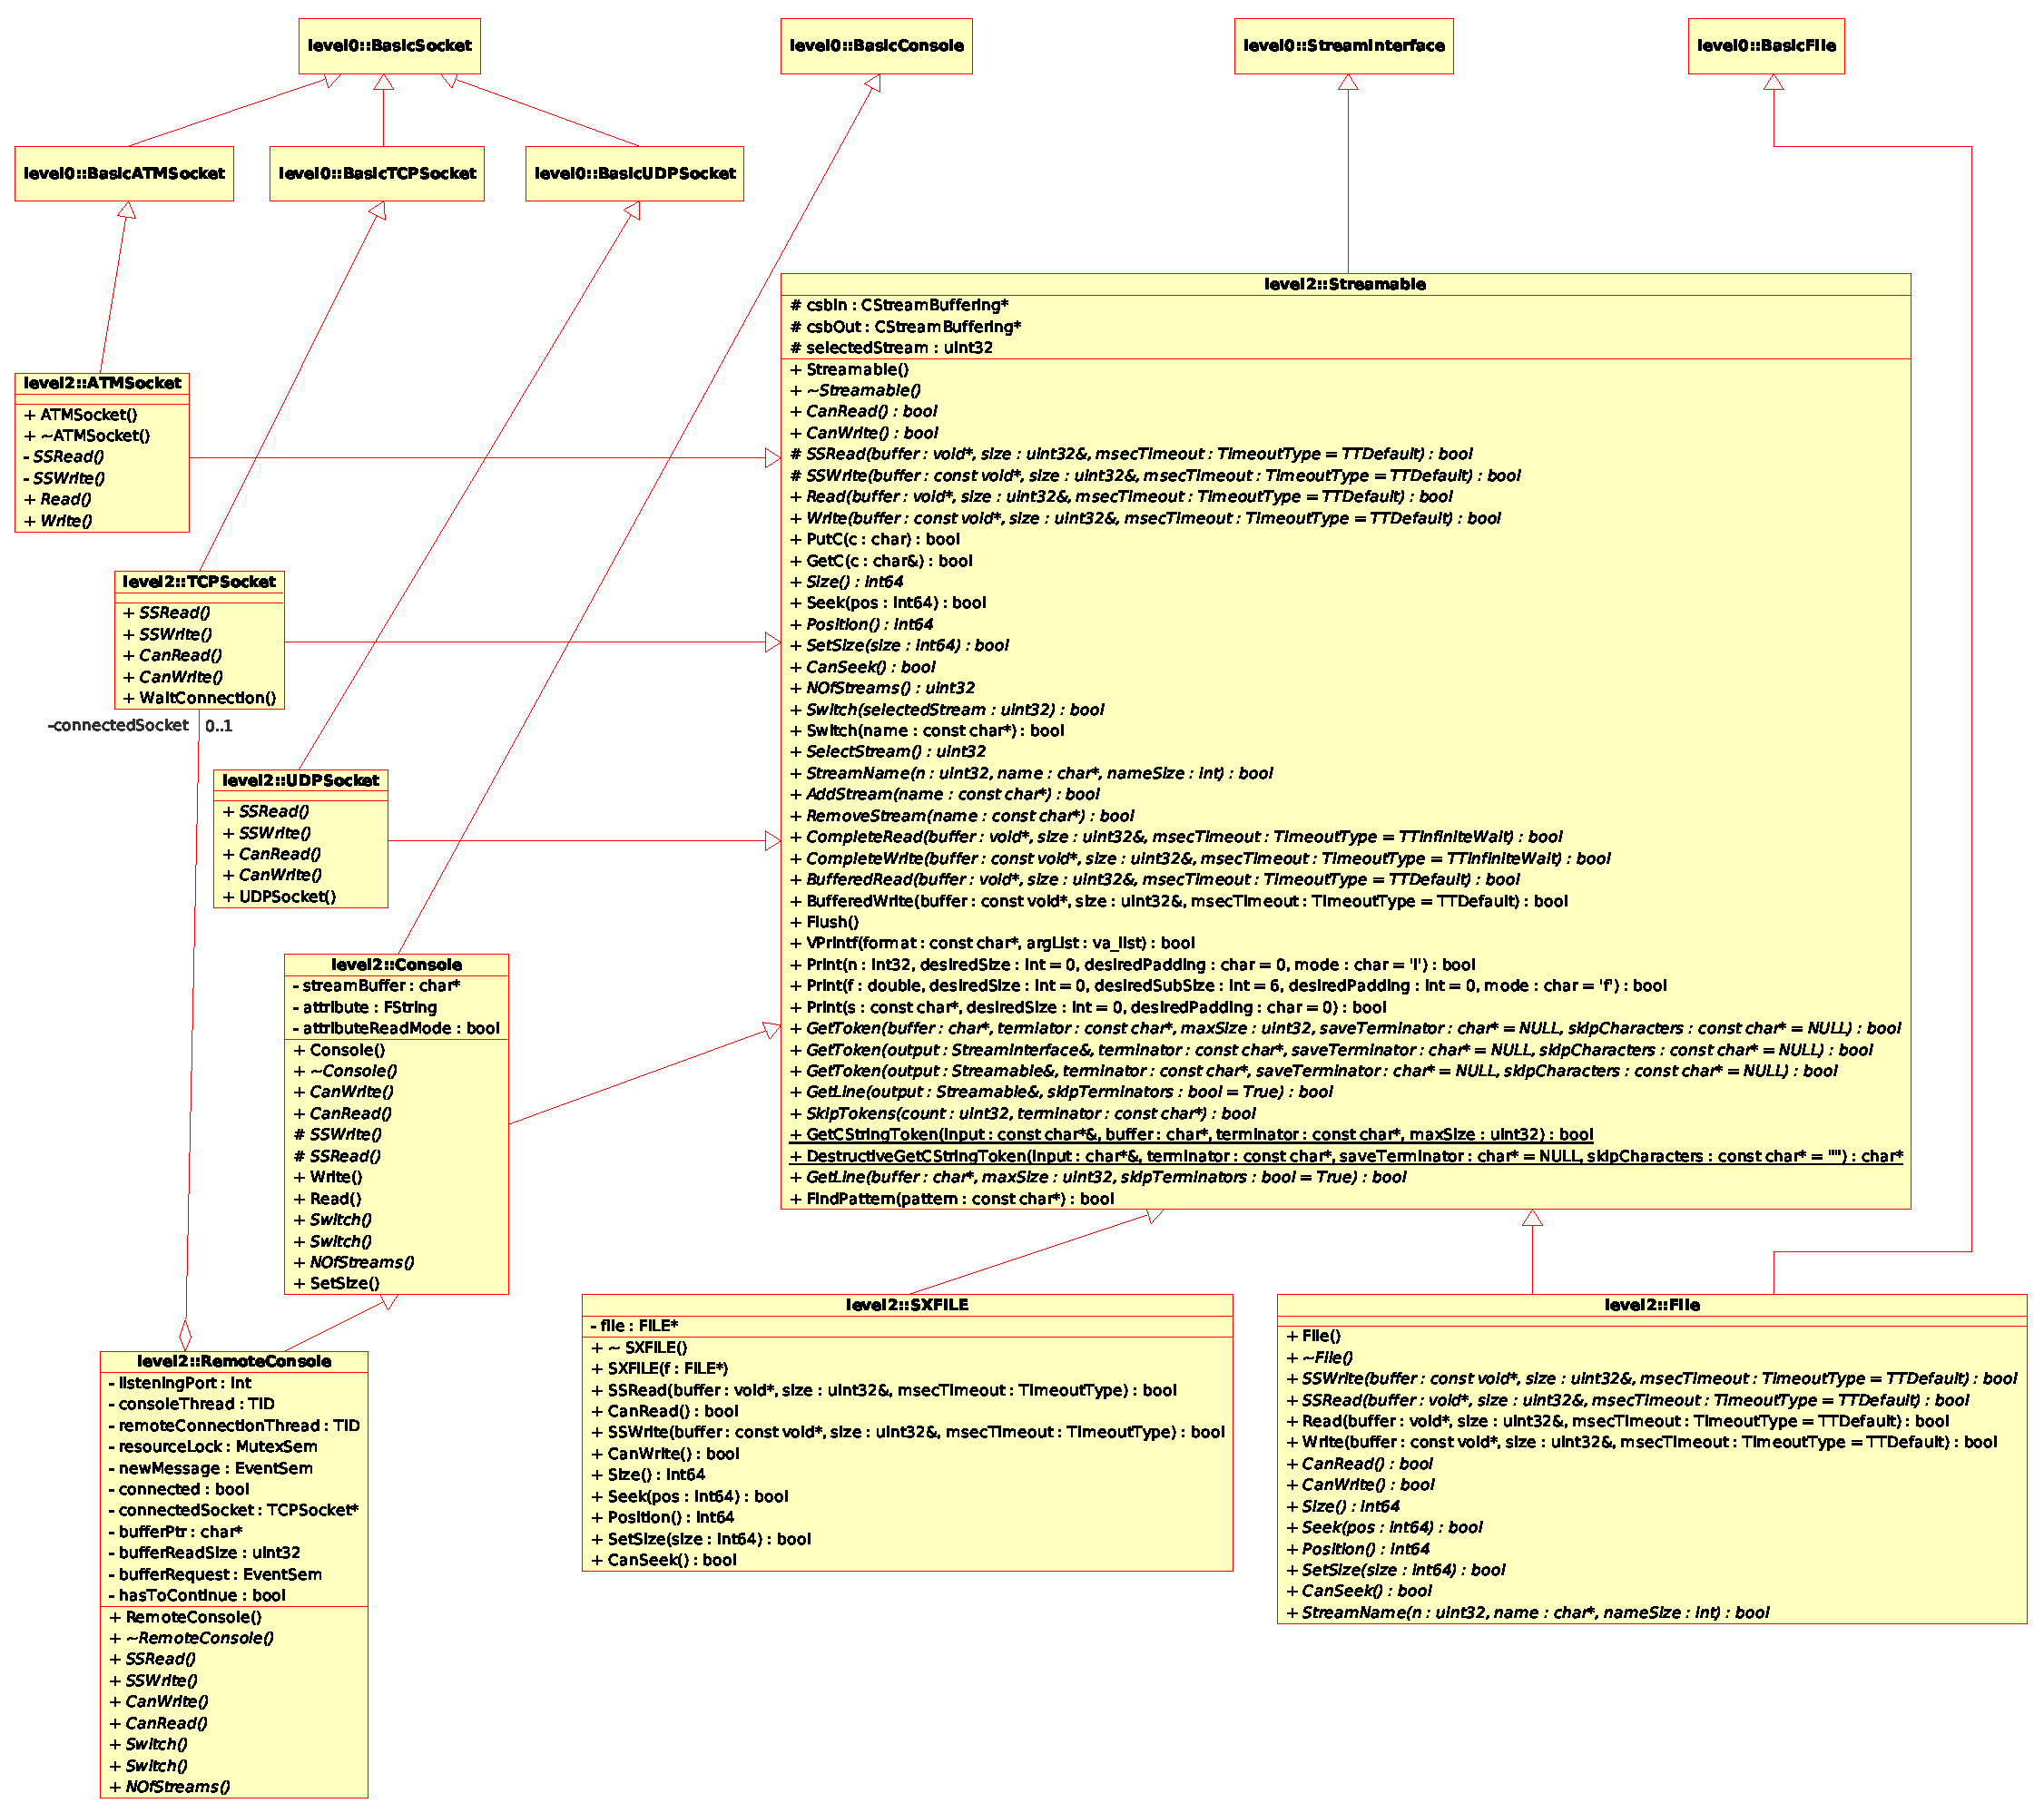
\includegraphics[width=\textwidth]{level2/level2-fstream.eps}
  \caption{BaseLib Level2 file streams classes}
  \label{f:level2:stream_file}
 \end{center}
\end{figure}

Class involved are listed below. Most of the classes are quite similar, classes can be groupped in three subcategories: network (sockets), console and file. But we doesn't follow this distintiction.
\begin{itemize}
 \item ATMSocket
 \item TCPSocket
 \item UDPSocket

 \item Console
 \item RemoteConsole

 \item File
 \item SXFILE
\end{itemize}



\subsubsection{ATMSocket}
\texttt{[ATMSocket.h, ATMSocket.cpp]}\\
The class \texttt{ATMSocket} adds the streamable capability to a \texttt{BasicATMSocket}, i.e. a \texttt{BasicATMSocket} can also be treat as a stream of data. In detail such class implements ATM sockets AAL5 layer.\\


The method \texttt{SSRead} reads a block of data from the socket, \texttt{size} is the maximum size, on return \texttt{size} is what was read, timeout is not supported yet. The method \texttt{SSWrite} writes a block of data: \texttt{size} is its size. Those methods call \texttt{BasicATMSocket} methods.

Last two methods call superclass methods.
\begin{lstlisting}[
extendedchars=true,%
basicstyle=\fontfamily{pcr}\fontseries{m}\selectfont\footnotesize, %
stepnumber=1,%
numberstyle=\tiny,%
keywordstyle=\footnotesize\tt ,%
language=C++]
public:
   ATMSocket(int32 socket=0);
   ~ATMSocket();

private:
   virtual bool SSRead(void* buffer,uint32& size,TimeoutType msecTimeout=TTDefault);
   virtual bool SSWrite(const void* buffer,uint32& size,TimeoutType msecTimeout=TTDefault);

public:
   virtual bool Read(void* buffer,uint32& size,TimeoutType msecTimeout=TTDefault);
   virtual bool Write(const void* buffer,uint32& size,TimeoutType msecTimeout=TTDefault);
\end{lstlisting}



\subsubsection{TCPSocket}
\texttt{[TCPSocket.h, TCPSocket.cpp]}\\
The class \texttt{TCPSocket} adds the streamable capability to a \texttt{BasicTCPSocket}, i.e. a \texttt{BasicTCPSocket} can also be treat as a stream of data. \\


Like in the previous \texttt{ATMSocket} class methods \texttt{SSRead} and \texttt{SSWrite} are overridden to make operations on the \texttt{BasicTCPSocket}. Methods \texttt{CanRead} and \texttt{CanWrite} are also overridden and return \texttt{true}.\\


The class adds also a new method to the \texttt{Streamable} class, the method is called \texttt{WaitConnection} and return a \texttt{TCPSocket*}, it simply wait for a new TCP connection and return the object holding the connection.
\begin{lstlisting}[
extendedchars=true,%
basicstyle=\fontfamily{pcr}\fontseries{m}\selectfont\footnotesize, %
stepnumber=1,%
numberstyle=\tiny,%
keywordstyle=\footnotesize\tt ,%
language=C++]
public:
   virtual bool SSRead(void* buffer,uint32& size,TimeoutType msecTimeout=TTDefault);
   virtual bool SSWrite(const void* buffer,uint32& size,TimeoutType msecTimeout=TTDefault);
   virtual bool CanRead();
   virtual bool CanWrite();

   TCPSocket* WaitConnection(TimeoutType msecTimeout = TTInfiniteWait,TCPSocket *client = NULL);
\end{lstlisting}



\subsubsection{UDPSocket}
\texttt{[UDPSocket.h, UDPSocket.cpp]}\\
The class \texttt{UDPSocket} adds the streamable capability to a \texttt{BasicUDPSocket}, i.e. a \texttt{BasicUDPSocket} can also be treat as a stream of data. This is quite uncommon to UDP based communication that are usually studied as a connectionless socket media.\\


Like in the previous classese methods \texttt{SSRead} and \texttt{SSWrite} are overridden to make operations on the \texttt{BasicUDPSocket}. Methods \texttt{CanRead} and \texttt{CanWrite} are also overridden and return \texttt{true}.
\begin{lstlisting}[
extendedchars=true,%
basicstyle=\fontfamily{pcr}\fontseries{m}\selectfont\footnotesize, %
stepnumber=1,%
numberstyle=\tiny,%
keywordstyle=\footnotesize\tt ,%
language=C++]
public:
   UDPSocket(int32 socket=0);

   virtual bool SSRead(void* buffer,uint32& size,TimeoutType msecTimeout=TTDefault);
   virtual bool SSWrite(const void* buffer,uint32& size,TimeoutType msecTimeout=TTDefault);
   virtual bool CanRead();
   virtual bool CanWrite();
\end{lstlisting}



\subsubsection{Console}
\texttt{[Console.h, Console.cpp]}\\
The class \texttt{Console} adds streaming capability to the class \texttt{BasicConsole}.

The first attribute, \texttt{streamBuffer}, is a small character array to buffer the console operations. On creation the constructor initialise che attribute \texttt{Streamble::csbIn} with the character array \texttt{streamBuffer} used as an buffered input.
\begin{lstlisting}[
extendedchars=true,%
basicstyle=\fontfamily{pcr}\fontseries{m}\selectfont\footnotesize, %
stepnumber=1,%
numberstyle=\tiny,%
keywordstyle=\footnotesize\tt ,%
language=C++]
private:
   char streamBuffer[32];
   FString attribute;
   bool attributeReadMode;
public:
   Console(ConsoleOpeningMode openingMode=ConsoleDefault,
      int numberOfColumns=-1,int numberOfRows=-1,TimeoutType msecTimeout=TTInfiniteWait);
   virtual ~Console();
\end{lstlisting}

Methods \texttt{CanWrite} and \texttt{CanRead} return both \texttt{true} because on a console you can either write and read. Methods \texttt{SSWrite} and \texttt{SSRead} supports different streams and are implemented to call \texttt{BasicConsole} methods or string related methods (\texttt{FString}).

Methods \texttt{Write} and \texttt{Read} call the superclass's method.

The first method \texttt{Switch} changes stream to write to, second method \texttt{Switch} is used to change the console attributes, valid names are ``colour'', two integers first is the fg second the bg; "cursor" the cursor position,  two integers X,Y; ``size'' the buffer size, two integers DX,DY and also ``window'' the window size, two integers DX,DY.
The method \texttt{NOfStreams} returns how many streams are available, and \texttt{SetSize} sets the size of the buffer.
\begin{lstlisting}[
extendedchars=true,%
basicstyle=\fontfamily{pcr}\fontseries{m}\selectfont\footnotesize, %
stepnumber=1,%
numberstyle=\tiny,%
keywordstyle=\footnotesize\tt ,%
language=C++]
   virtual bool CanWrite();
   virtual bool CanRead();
protected:
   virtual bool SSWrite(const void* buffer,uint32& size,TimeoutType msecTimeout=TTDefault);
   virtual bool SSRead(void* buffer,uint32& size,TimeoutType msecTimeout=TTDefault);
public:
   inline bool Write(const void* buffer,uint32& size,TimeoutType msecTimeout=TTDefault);
   inline bool Read(void* buffer,uint32& size,TimeoutType msecTimeout=TTDefault);

   virtual bool Switch(uint32 newSelectedStream);
   virtual bool Switch(const char *name);
   virtual uint32 NOfStreams();
   inline bool SetSize(int numberOfColumns,int numberOfRows);
\end{lstlisting}



\subsubsection{RemoteConsole}
\texttt{[RemoteConsole.h, RemoteConsole.cpp]}\\
The class \texttt{RemoteConsole} simulates a \texttt{Console} for all purposes but allows a remote connection to take over. The \texttt{RemoteConsole} adds the possibility to connect a console via a TCP channel, inthis way we obtain a remote console; the remote connection is made available via a \texttt{TCPSocket} object hold as an attribute. \\


The \texttt{RemoteConsole} works with the aim of two threads: one that transmit and receive data on the TCP path and the other that handle local console commands (have a look at \textit{level2/RemoteConsole.cpp}.

There are many attributes, most of them are semaphore or mutexes and are needed to keep synchronized the two threads.
\begin{lstlisting}[
extendedchars=true,%
basicstyle=\fontfamily{pcr}\fontseries{m}\selectfont\footnotesize, %
stepnumber=1,%
numberstyle=\tiny,%
keywordstyle=\footnotesize\tt ,%
language=C++]
private:
   int listeningPort;
   TID consoleThread;
   TID remoteConnectionThread;
   MutexSem resourceLock;
   EventSem newMessage;
   bool connected;
   TCPSocket* connectedSocket;
   char* bufferPtr;
   uint32 bufferReadSize;
   EventSem bufferRequest;
   bool hasToContinue;
\end{lstlisting}

The constructor initialize the object and bind the TCP socket listening on port 32769 (default) for incoming \texttt{RemoteConsole} connections, in this way an extarnal user can connect itself to the system simply connecting to that port on an host using a program like \texttt{telnet} and has a remote console to interact with BaseLib.
\begin{lstlisting}[
extendedchars=true,%
basicstyle=\fontfamily{pcr}\fontseries{m}\selectfont\footnotesize, %
stepnumber=1,%
numberstyle=\tiny,%
keywordstyle=\footnotesize\tt ,%
language=C++]
public:
   RemoteConsole(int listeningPort=32769);
   virtual ~RemoteConsole();

   virtual bool SSRead(void* buffer,uint32& size,TimeoutType msecTimeout=TTDefault);
   virtual bool SSWrite(const void* buffer,uint32& size,TimeoutType msecTimeout=TTDefault);
   virtual bool CanWrite();
   virtual bool CanRead();
   
   virtual bool Switch(uint32 selectedStream);
   virtual bool Switch(const char* name);
   virtual uint32 NOfStreams();
\end{lstlisting}



\subsubsection{File}
\texttt{[File.h, File.cpp]}\\
The class \texttt{File} adds the streamable capability to a \texttt{BasicFile}, i.e. a \texttt{BasicFile} can also be treat as a stream of data.\\

Methods \texttt{SSRead} and \texttt{SSWrite} call \texttt{BasicFile}'s methods to read and write to the file; \texttt{Read} and \texttt{Write} are overridden but do the same as declared in the \texttt{Streamable} superclass, we can said the same for all other methods except \texttt{CanRead} and \texttt{CanWrite} that simply return \texttt{true} and the last method.

The method \texttt{StreamName} returns the file name or the name of any other substream we are using.
\begin{lstlisting}[
extendedchars=true,%
basicstyle=\fontfamily{pcr}\fontseries{m}\selectfont\footnotesize, %
stepnumber=1,%
numberstyle=\tiny,%
keywordstyle=\footnotesize\tt ,%
language=C++]
public:
   virtual bool SSRead(void* buffer,uint32& size,TimeoutType msecTimeout=TTDefault);
   virtual bool SSWrite(const void* buffer,uint32& size,TimeoutType msecTimeout=TTDefault);

   inline bool Read(void* buffer,uint32& size,TimeoutType msecTimeout=TTDefault);
   inline bool Write(const void* buffer,uint32& size,TimeoutType msecTimeout=TTDefault);

   virtual bool CanRead();
   virtual bool CanWrite();

   virtual int64 Size();
   virtual bool SetSize(int64 size);
   virtual bool Seek(int64 pos);
   virtual int64 Position(void);
   virtual bool CanSeek();

   virtual bool StreamName(uint32 n,char* name,int nameSize);
\end{lstlisting}



\subsubsection{SXFILE}
\texttt{[SX\_File.h]}\\
Class \texttt{SXFILE} inherits only from \texttt{Streamable} (not also from \texttt{BasicFile} like class \texttt{File}). The class \texttt{SXFILE} is a \textit{Streamable eXtension} for the standard C \texttt{FILE} routines.\\


Basically this class has as an attribute an integer that is nothing more than a file descriptor, on this file descriptor, that must be passed as an argument to the constructor, the class acts on standard C library function as \texttt{fwrite}, \texttt{fread}, \texttt{ftell} and \texttt{fseek} to implement a file streaming interface.
The class must be completed with a new constructor that handle also file creation or opening.
\begin{lstlisting}[
extendedchars=true,%
basicstyle=\fontfamily{pcr}\fontseries{m}\selectfont\footnotesize, %
stepnumber=1,%
numberstyle=\tiny,%
keywordstyle=\footnotesize\tt ,%
language=C++]
private:
   int file;
public:
   virtual ~SXFILE();
   SXFILE(int f);

   bool SSRead(void* buffer, uint32 &size,TimeoutType msecTimeout);
   bool SSWrite(const void* buffer, uint32 &size,TimeoutType msecTimeout);
   bool CanRead();
   virtual bool CanWrite();

   int64 Size();
   bool SetSize(int64 size);
   bool  Seek(int64 pos);
   int64 Position(void);
   virtual bool CanSeek();
\end{lstlisting}



\subsection{Design Notes}
Some notes about constructors, if a constructor fail it must throw an exception, if doesn't throws an exception one can think that all its going well and after a while exeprience a bug. It is probably necessary to write some exception mechanism for example in \texttt{BufferedStream} if the argument is \texttt{NULL} then the object doesn't create itself and exit from the constructor. In class \texttt{SXMemory} the constructor doesn't check arguments.\\


There is a security hole in the \texttt{RemoteConsole}, is a TCP remote connection and doesn't check against password and autentication, use it with care because if the port is publically exposed some DOS attack can be experience.



\section{ConfigurationDataBase}
As we said in the previous chapters the ConfigurationDataBase is one of the key elements in the BaseLib software infrastructure. In Figure \ref{f:level2:CDB} is depicted the UML related to the classes in this level.
\begin{figure}[h!]
 \begin{center}
  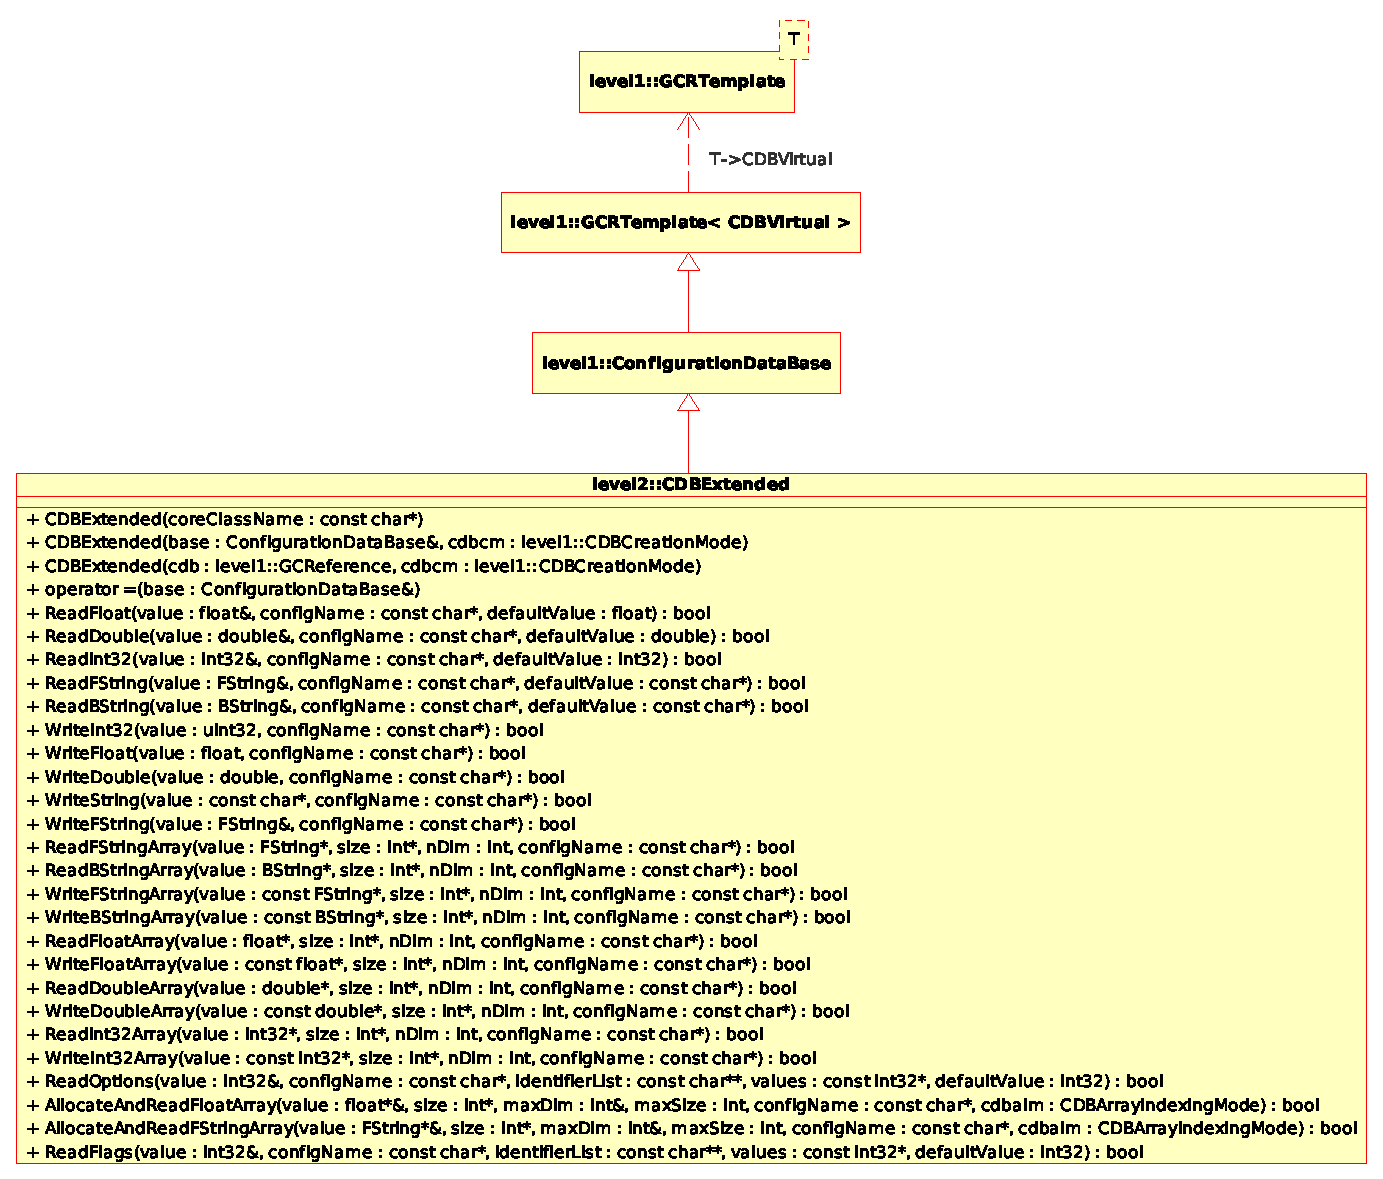
\includegraphics[width=0.83\textwidth]{level2/level2-CDB.eps}
  \caption{BaseLib Level2 CDB classes}
  \label{f:level2:CDB}
 \end{center}
\end{figure}

Basically there is only one class: \texttt{CDBExtended}. This class is an extension to the ConfigurationDataBase class; contains a reference to CDB of type CDBVirtual Forces call to CDB to be made via the virtual table.
Sources, in this group, regarding level2 are:
\begin{itemize}
 \item CDBExtended.h
 \item CDBDataTypes.h
 \item CDBDataTypes.cpp
\end{itemize}

In the following we analyse the \texttt{CDBExtended} class that will simply extends the \texttt{ConfigurationDataBase} with many specialized read and write methods. Such class is written as a collection of inline methods, also constructors are declared as \texttt{inline}.

The first constructor create a CDB from a generic base type, i.e. it will create a new \texttt{CDBNull} and than sets some value. The second constructor if \texttt{base} is specified it creates a new reference to an existing database, \texttt{cdbcm} attribute if is set to \texttt{CDBCM\_CopyAddress} copies the address from the reference. The last constructor is similar to the second one. The copy operator of a CDB creates a new reference to an existing database.\\

\begin{lstlisting}[
extendedchars=true,%
basicstyle=\fontfamily{pcr}\fontseries{m}\selectfont\footnotesize, %
stepnumber=1,%
numberstyle=\tiny,%
keywordstyle=\footnotesize\tt ,%
language=C++]
public:
   inline CDBExtended(const char* coreClassName="CDB")
   inline CDBExtended(ConfigurationDataBase& base,CDBCreationMode cdbcm=CDBCM_CopyAddress);
   inline CDBExtended(GCReference cdb,CDBCreationMode cdbcm=CDBCM_CopyAddress);

   inline void operator=(ConfigurationDataBase& base);
\end{lstlisting}

Next methods address the read and write activity, read methods simply call \texttt{CDBVirtual::ReadArray} and write methods call \texttt{CDBVirtual::WriteArray}. All that with different arguments to read/write \texttt{Float}, \texttt{Double}, \texttt{Int32}, \texttt{FString}, \texttt{BString}, \texttt{FStringArray}, \texttt{BStringArray}, \texttt{FloatArray}, \texttt{DoubleArray} and \texttt{Int32Array}.
\begin{lstlisting}[
extendedchars=true,%
basicstyle=\fontfamily{pcr}\fontseries{m}\selectfont\footnotesize, %
stepnumber=1,%
numberstyle=\tiny,%
keywordstyle=\footnotesize\tt ,%
language=C++]
   inline bool ReadFloat(float &value,const char* configName,float defaultValue = 0);
   inline bool ReadDouble(double &value,const char* configName,double defaultValue = 0);
   inline bool ReadInt32(int32 &value,const char* configName,int32 defaultValue = 0);
   inline bool ReadFString(FString &value,const char* configName,const char *defaultValue = "");
   inline bool ReadBString(BString &value,const char* configName,const char *defaultValue = "");
   inline bool ReadFStringArray(FString* value,int* size,int nDim,const char* configName);
   inline bool ReadBStringArray(BString* value,int* size,int nDim,const char* configName);
   inline bool ReadFloatArray(float* value,int* size,int nDim,const char* configName);
   inline bool ReadDoubleArray(double* value,int* size,int nDim,const char* configName);
   inline bool ReadInt32Array(int32* value,int* size,int nDim,const char* configName);

   inline bool WriteFloat(float value,const char* configName);
   inline bool WriteDouble(double value,const char* configName);
   inline bool WriteInt32(uint32 value,const char* configName);
   inline bool WriteFString(FString &value,const char* configName);
   inline bool WriteString(const char *value,const char* configName);
   inline bool WriteFStringArray(const FString* value,int* size,int nDim,const char* configName);
   inline bool WriteBStringArray(const BString* value,int* size,int nDim,const char* configName);
   inline bool WriteFloatArray(const float* value,int* size,int nDim,const char* configName);
   inline bool WriteDoubleArray(const double* value,int* size,int nDim,const char* configName);
   inline bool WriteInt32Array(const int32* value,int* size,int nDim,const char* configName);
\end{lstlisting}

The method \texttt{ReadOptions} translates an identifier to a value, \texttt{dentifierList} is a zero terminated vector of \texttt{const char*}.
The method \texttt{ReadFlags} translates a vector of identifiers to a bitset value, \texttt{identifierList} is a zero terminated vector of \texttt{const char*} the values associated to each identifier is in \texttt{values}.

The method \texttt{AllocateAndReadFloatArray} finds the matrix dimension first then allocates memory and finally read data; \texttt{size} parameter is a vector of dimensions of size \texttt{maxDim}; \texttt{value} argument will be allocated with at maximum \texttt{maxSize} floats, this routine uses malloc. The method \texttt{AllocateAndReadFStringArray} does exactly the same but handles \texttt{FString} objects; \texttt{value} argument will be allocated with at maximum \texttt{maxSize} \texttt{FString}, this routine used \texttt{new[]}.
\begin{lstlisting}[
extendedchars=true,%
basicstyle=\fontfamily{pcr}\fontseries{m}\selectfont\footnotesize, %
stepnumber=1,%
numberstyle=\tiny,%
keywordstyle=\footnotesize\tt ,%
language=C++]
   inline bool ReadOptions(int32& value,
      const char* configName,
      const char** identifierList,
      const int32* values,
      int32 defaultValue);
   inline bool ReadFlags(int32& value,
      const char* configName,
      const char** identifierList,
      const int32* values,
      int32 defaultValue);

   inline bool AllocateAndReadFloatArray(float*& value,int* size,int& maxDim,int maxSize,
      const char* configName,CDBArrayIndexingMode cdbaim=CDBAIM_Strict);
   inline bool AllocateAndReadFStringArray(FString*& value,int* size,int& maxDim,int maxSize,
      const char* configName,CDBArrayIndexingMode cdbaim=CDBAIM_Strict)
\end{lstlisting}



\subsection{Design Notes}
---



\section{IO devices}
In Level2 there are also two input device classes. Those input devices classes are: the serial line and the keyboard. In Figure \ref{f:level2:Input} the UML schema is depicted.

\begin{figure}[h!]
 \begin{center}
  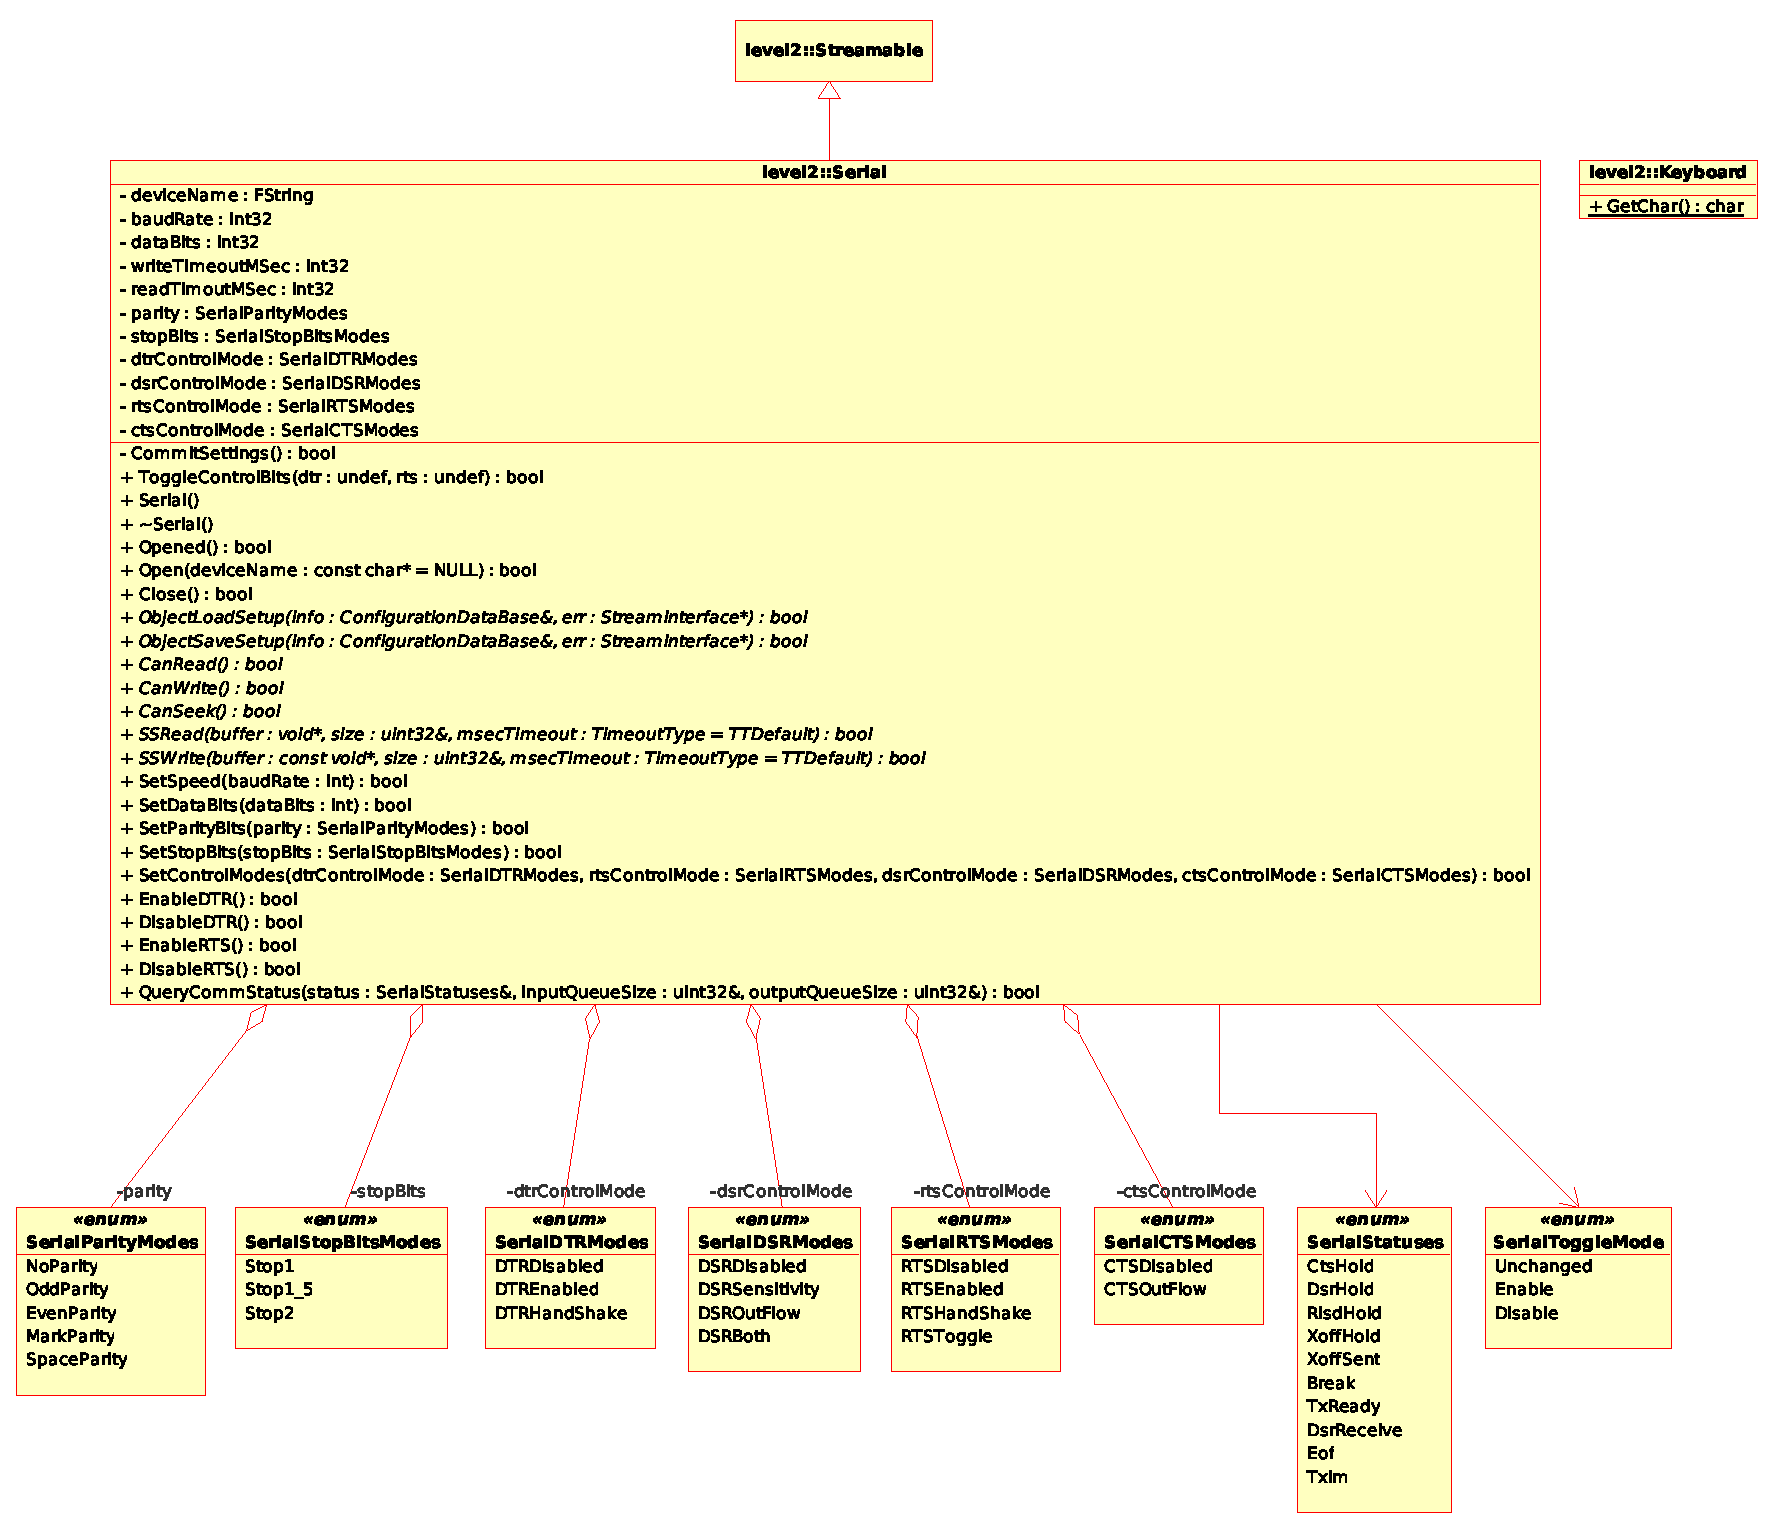
\includegraphics[width=0.83\textwidth]{level2/level2-Input.eps}
  \caption{BaseLib Level2 Input devices classes}
  \label{f:level2:Input}
 \end{center}
\end{figure}

We speak brefily about the \texttt{Keyboard} class than we take a tour of the serial line implementation that is much more interesting and better developed.



\subsubsection{Keyboard}
\texttt{[Keyboard.h]}\\
The \texttt{Keyboard} class manages the direct access to keyboard. The access is done throught a library call, in most UNIX like system the call is \texttt{getchar()}, from the standard C library, in all other system \texttt{\_getch} is used. The result is a read operation of a char without echoing. The straightforward implementation follow.

Note that this class doesn't interface directly with a driver but relay on the Operating System and C libraries.
\begin{lstlisting}[
extendedchars=true,%
basicstyle=\fontfamily{pcr}\fontseries{m}\selectfont\footnotesize, %
stepnumber=1,%
numberstyle=\tiny,%
keywordstyle=\footnotesize\tt ,%
language=C++]
class Keyboard{
public:
#if !(defined(_VXWORKS)||defined(_RTAI)|| defined(_LINUX) || defined(_SOLARIS))
    static  char GetChar() {return _getch();}
#else
    static char GetChar() {return getchar();}
#endif
};
\end{lstlisting}



\subsubsection{Serial}
\texttt{[Serial.h, Serial.cpp]}\\
The class \texttt{Serial} inherits from \texttt{Streamable}, i.e. the serial line can also be treated as a stream of data.\\


The class \texttt{Serial} in some OSes needs a file handle, attribute \texttt{port}, in the class is just defined for OS/2 and Microsoft Windows. The name of the device, the path in some systems, is hold by the \texttt{deviceName} attribute, all other attributes are serial line common properties and settings.
\begin{lstlisting}[
extendedchars=true,%
basicstyle=\fontfamily{pcr}\fontseries{m}\selectfont\footnotesize, %
stepnumber=1,%
numberstyle=\tiny,%
keywordstyle=\footnotesize\tt ,%
language=C++]
#if defined (_OS2)
    HFILE port;
#elif defined (_WIN32)
    HANDLE port;
#endif
   FString deviceName;
   int32 baudRate;
   int32 dataBits;
   int32 writeTimeoutMSec;
   int32 readTimeoutMSec;
   SerialParityModes parity;
   SerialStopBitsModes stopBits;
   SerialDTRModes dtrControlMode;
   SerialDSRModes dsrControlMode;
   SerialRTSModes rtsControlMode;
   SerialCTSModes ctsControlMode;
\end{lstlisting}

The method \texttt{CommitSettings} implements all the programmed changes, some methods only affects class's attributes and calling the method doesn't directly affect the serial line. \texttt{ToggleControlBits} changes the status of \textit{dtr} and \textit{rts} control lines in the serial interface, a value of \texttt{0} means untouched, \texttt{1} means to turn on and \texttt{2} means to turn off.\\


The method \texttt{Opened} query if the serial line device is just opened or not; \texttt{Open} open the device specified in the \texttt{name} argument, the name can be also a path in UNIX, in Microsoft Windows is something like \texttt{COM1}, if \texttt{name} argument is \texttt{NULL} than it will open what was setup using \texttt{ObjectLoadSetup}; \texttt{Close} closes the device.\\


The method \texttt{ObjectLoadSetup} accept from the configuration file the following parameters:
\begin{lstlisting}[
extendedchars=true,%
basicstyle=\fontfamily{pcr}\fontseries{m}\selectfont\footnotesize, %
stepnumber=1,%
numberstyle=\tiny,%
keywordstyle=\footnotesize\tt ,%
language=bash]
   DeviceName COM1:
      BaudRate   int
      DataBits   5 6 7 8 9
      WriteTimeoutMSec   int
      ReadTimeoutMSec   int
      Parity   NoParity OddParity EvenParity MarkParity SpaceParity
      StopBits   Stop1 Stop1_5 Stop2
      RTSControlMode   RTSDisabled RTSEnabled RTSToggle
      DTRControlMode   DTRDisabled DTREnabled DTRHandShake
      DSRControlMode   DSRDisabled DSRSensitivity DSROutFlow DSRBoth
      CTSControlMode   CTSDisabled CTSOutFlow
\end{lstlisting}

The method \texttt{ObjectSaveSetup} is the standard object save function.

Methods\texttt{CanRead} and \texttt{CanWrite} return \texttt{true}; the method \texttt{CanSeek} is not available and return \texttt{false}.
The method \texttt{SSRead} reads a block of data, \texttt{size} is the maximum size, on return \texttt{size} is what was read, the timeout is not supported yet. \texttt{SSWrite} writes a block of data,  \texttt{size} is its size, on return \texttt{size} is what was written.
\begin{lstlisting}[
extendedchars=true,%
basicstyle=\fontfamily{pcr}\fontseries{m}\selectfont\footnotesize, %
stepnumber=1,%
numberstyle=\tiny,%
keywordstyle=\footnotesize\tt ,%
language=C++]
private:
   inline bool CommitSettings();
   inline bool ToggleControlBits(SerialToggleMode dtr, SerialToggleMode rts);

public:
   Serial();
   ~Serial();

   bool Opened();
   bool Open(const char *deviceName=NULL);
   bool Close();

   virtual bool ObjectLoadSetup(ConfigurationDataBase &info,StreamInterface *err);
   virtual bool ObjectSaveSetup(ConfigurationDataBase& info,StreamInterface* err);

   virtual bool CanRead();
   virtual bool CanWrite();
   virtual bool CanSeek();

   virtual bool SSRead(void* buffer,uint32& size,TimeoutType msecTimeout=TTDefault);
   virtual bool Write(const void* buffer,uint32& size,TimeoutType msecTimeout=TTDefault);
\end{lstlisting}

The following function lets the user set the serial line parameters and to enable them.
Last method \texttt{QueryCommStatus} retrieves the status of communication port.
\begin{lstlisting}[
extendedchars=true,%
basicstyle=\fontfamily{pcr}\fontseries{m}\selectfont\footnotesize, %
stepnumber=1,%
numberstyle=\tiny,%
keywordstyle=\footnotesize\tt ,%
language=C++]
   bool SetSpeed(int baudRate);
   bool SetDataBits(int dataBits);
   bool SetParityBits(SerialParityModes parity);
   bool SetStopBits(SerialStopBitsModes stopBits);

   bool SetControlModes(
        SerialDTRModes dtrControlMode,
        SerialRTSModes rtsControlMode,
        SerialDSRModes dsrControlMode,
        SerialCTSModes ctsControlMode);

   inline bool EnableDTR(void);
   inline bool DisableDTR(void);
   inline bool EnableRTS(void);
   inline bool DisableRTS(void);

   inline bool QueryCommStatus(SerialStatuses& status,
      uint32& inputQueueSize,
      uint32& outputQueueSize);
\end{lstlisting}



\subsection{Design Notes}
The class \texttt{Serial} is a \texttt{Streamable} object, but, is not likely to be a real stream of data, it is more an i/o device (why not an IOGAM..) or something architectural dependent, the same can be said for the \texttt{Keyboard} class.

The class \texttt{Keyboard} must be better developed without the need of the C standard library; an architectural dependent keyboard code can be developed to doesn't relay on the OS itself.




\chapter{BaseLib Level 3}
\chaptermark{Level 3}


BaseLib Level 3 deals about the problem of configuration that is really similar to serialization in Object Oriented Programming (OOP) in BaseLib. The basic issue addressed here is the reding and writing of a configuration file from a file or generally from a stream, the stream is a formatted document where it is saved a configuration of the system, a configuration must also be thinked as a backed up set of instances of all the classes in a particular life moment of the system (OOP serialization). \\


The main tool that lets the user select which class to load and setting the parameters is the \textit{Configuration Database}, a \textit{Configuration Database}, that was just partially covered in the previous chapters, is a tree data structure that reflect the content of a configuration file (or stream). Using this philosopy every component of the framework that need configuration parameters must ask to this central entity that address configuration issues. \\


The whole BaseLib Level 3 could be divided in the following sections:
\begin{itemize}
 \item CDB
 \item other CDBs (stream oriented CDBs)
 \item Parser
\end{itemize}

The fundamental component of this level is the CDB, i.e. an implementation of a \texttt{Configuration Database} interface in \textit{/level1}. A CDB addresses the problem of which classes and which paramenters loading during the framework startup and reflect the system status (i.e. instantiated classes and attributes value) not only at the initialization but also during runtime; i.e. implements serialization.

Objects type registration and object instantiation is done by the previously analized GODB and ORDB; configuration database loading is the last step for the system inizialization. \\


The flow chart in Figure \ref{f:level3:objects} shows the order in which the logical components that compose the objects infrastructure, i.e. type registration, instantiation and serialization; are loaded by the BaseLib framework at application startup.

Loading an application that runs under the BaseLib framework lets the code first execute the compile time C++ code that create static and globally defined classes; part of this classes create the ORDB. Then a configuration file (or a stream) will be read and a configuration tree will be created, i.e. a CDB. When the ORDB and the CDB are ready a GODB is then filled up using the configuration of a CDB loading objects registered in the ORDB. This is the whole story; we try to better explain all this stuff with an example in the following. \\

\begin{figure}[h!]
 \begin{center}
  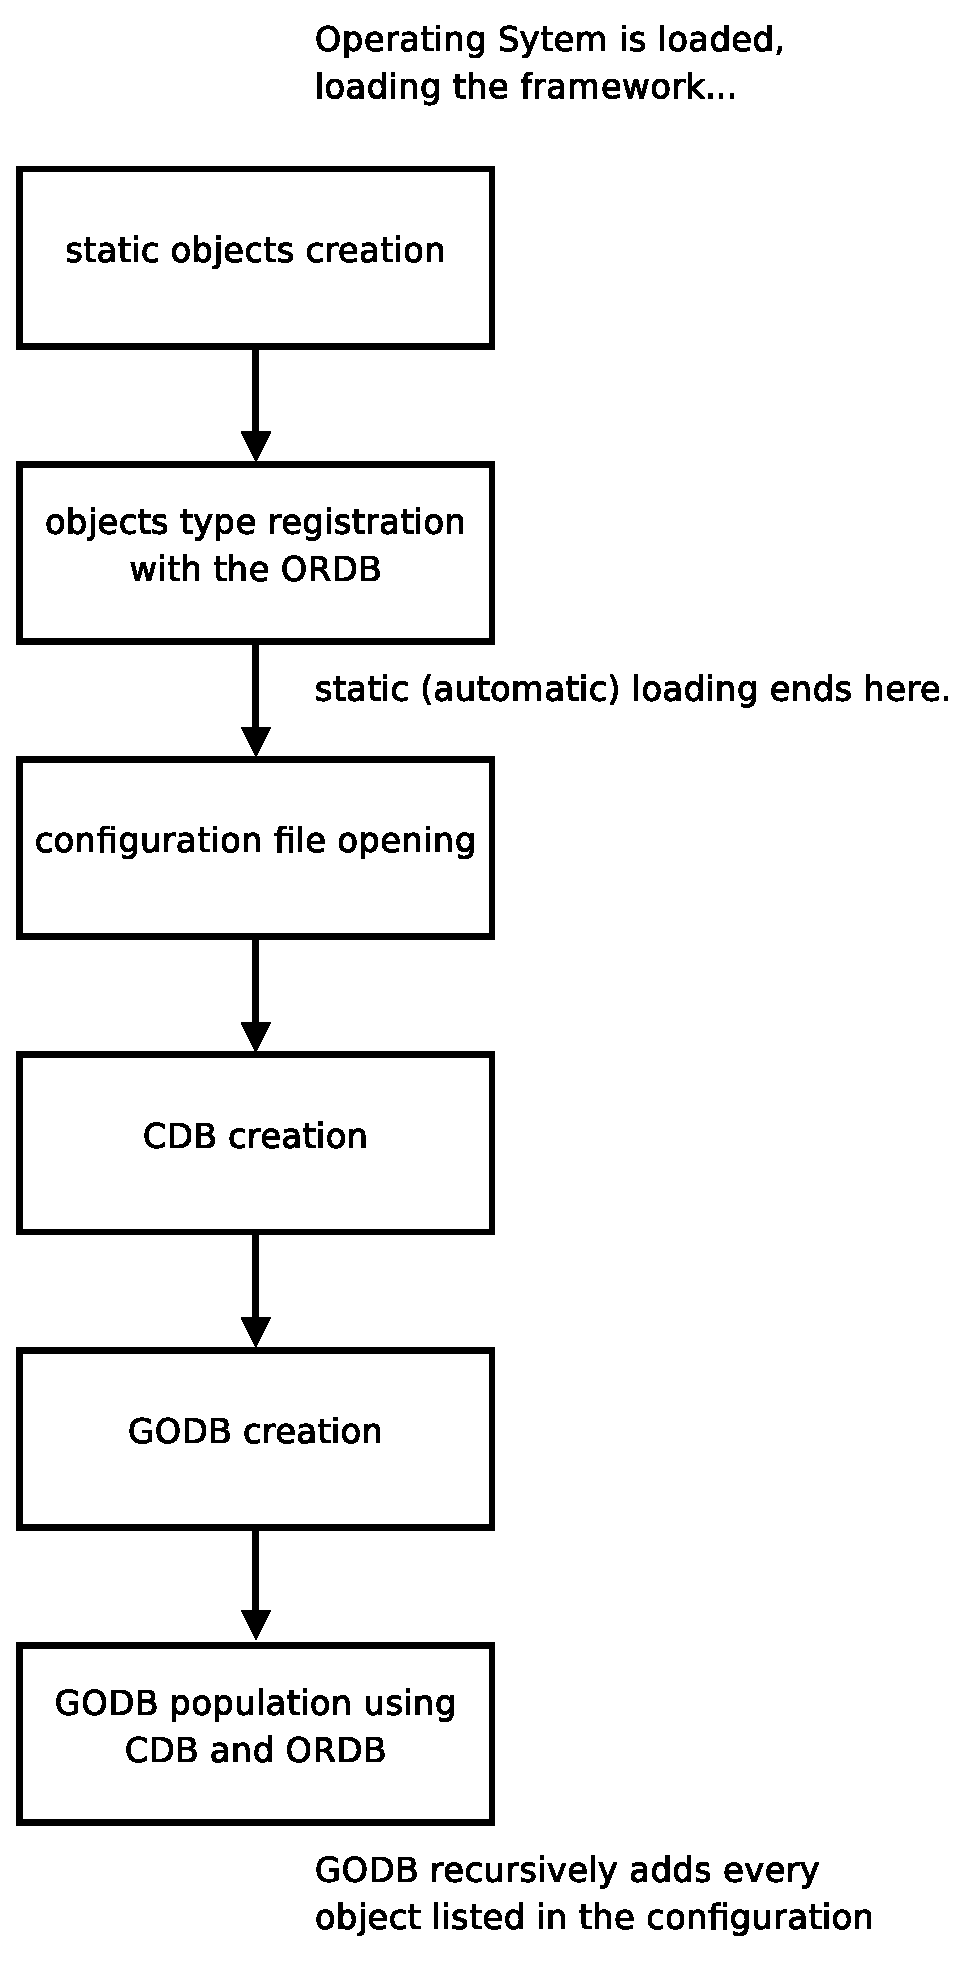
\includegraphics[width=0.33\textwidth]{level3/objects.eps}
  \caption{BaseLib objects loading and instantiation sequence}
  \label{f:level3:objects}
 \end{center}
\end{figure}



\paragraph{Example}
We now have a look to a simple example that make use of BaseLib and instantiate its objects via the CDB, the example is located in \textit{BaseLibTests/TestMessageBroker.cpp}. The first thing that follow is a snippets of a C++ source where there is the configuration data as a \texttt{char*} string. Don't try to understand what kind of objects are represented, they are no meaning in this place, have a look to the string format and try to understand the insights.

\begin{lstlisting}[
extendedchars=true,%
basicstyle=\fontfamily{pcr}\fontseries{m}\selectfont\footnotesize, %
stepnumber=1,%
numberstyle=\tiny,%
keywordstyle=\footnotesize\tt ,%
language=C++]
const char* testMessageBroker=
   "+TREES={"
   "    Class = GCReferenceContainer\n"
   "   +BRANCH1={\n"
   "        Class = GCReferenceContainer\n"
   "       +EP1={\n"
   "           Class = MessageEndPoint\n"
   "       }\n"
   "   }\n"
   "   +BRANCH2={\n"
   "        Class = GCReferenceContainer\n"
   "       +EP2={\n"
   "           Class = MessageEndPoint\n"
   "       }\n"
   "   }\n"
   "   +BRANCH3={\n"
   "        Class = MessageBroker\n"
   "        PeerIpAddress = localhost\n"
   "        PeerPort = 8882\n"
   "   }\n"
   "}\n"
   "+MC={\n"
   "    Class = MessageSenderTest\n"
   "}\n"
   "+MS={\n"
   "    Class = MessageServer\n"
   "    ServerPort = 8881\n"
   "}\n";
\end{lstlisting}

Now we follow the process of the objects creation starting from the previous string configuration. All the process, in the source behind is depicted, using a UML diagram, in Figure \ref{f:level3:TestMessageBroker}. The basic steps are: creating a stream of data, in this case an \texttt{SXMemory} object, create a \texttt{ConfigurationDataBase} object, that is a \texttt{GRTemplate} templatized on any \texttt{CDBVirtual}, in this case a \texttt{CDB} that we will analize in this chapter and then the \texttt{cdb} is passed to the GODB for class instantiation.

\begin{lstlisting}[
extendedchars=true,%
basicstyle=\fontfamily{pcr}\fontseries{m}\selectfont\footnotesize, %
stepnumber=1,%
numberstyle=\tiny,%
keywordstyle=\footnotesize\tt ,%
language=C++]
   SXMemory config((char*)testMessageBroker,strlen(testMessageBroker));
   ConfigurationDataBase cdb;
   if(!cdb->ReadFromStream(config,NULL)){
      CStaticAssertErrorCondition(ParametersError,"Init: cdb.ReadFromStream failed");
      return -1;
   }

   GCRTemplate<GCReferenceContainer> godb = GetGlobalObjectDataBase();
   godb->ObjectLoadSetup(cdb,NULL);
\end{lstlisting}

Creating a automatic class \texttt{ConfigurationDataBase} as we can see in Figure \ref{f:level3:TestMessageBroker}, let an automatic chain of constructor take place that construct defaulty a ConfigurationDataBase of type \texttt{CDB} that is the first issue addressed in this chapter.
\begin{figure}[h!]
 \begin{center}
  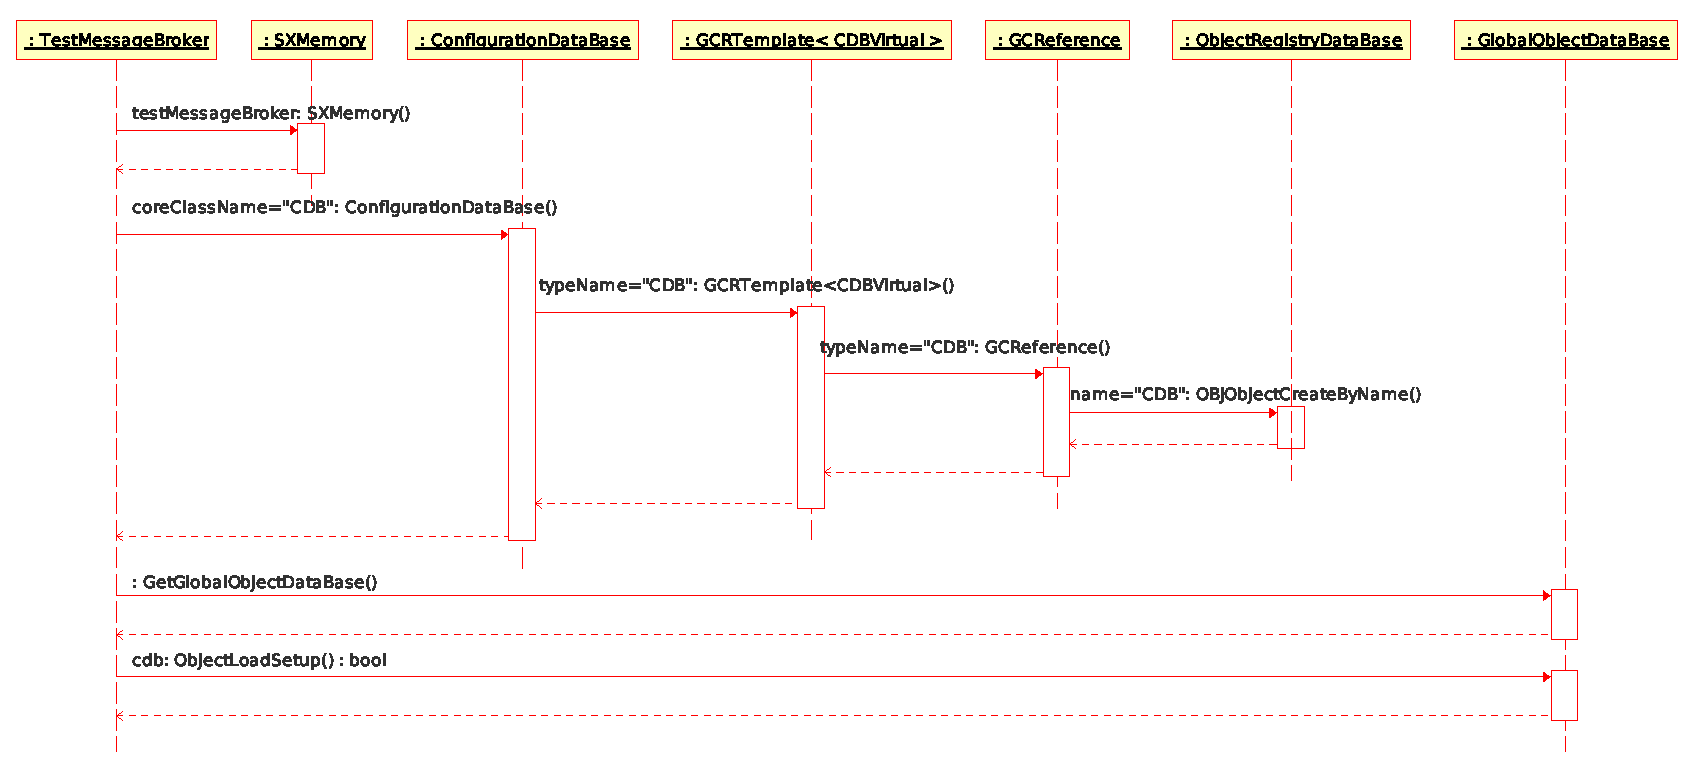
\includegraphics[width=\textwidth]{level3/TestMessageBroker.eps}
  \caption{BaseLib TestMessageBroker example}
  \label{f:level3:TestMessageBroker}
 \end{center}
\end{figure}

We end this introductory paragraph with another example of a configuration file. Those lines can be cut and pasted in a single file ending in \texttt{.cfg}.
\begin{lstlisting}[
extendedchars=true,%
basicstyle=\fontfamily{pcr}\fontseries{m}\selectfont\footnotesize, %
stepnumber=1,%
numberstyle=\tiny,%
keywordstyle=\footnotesize\tt ,%
language=bash]
+HttpServer = {
   Class = HttpService
   Port = 8084
}
+Control = {
   Class = ControlGAM
   Controller = {
      NoPlasmaVelocityGain = 0.0
      NoPlasmaCurrentGain = 40.0
         IPWaveform = {
            Times = {0 120}
            Amplitudes = {0.5 0.5}
            Rounding = 50
         }
   }
}
+DAM = {
   Class = DAMGAM
   // Projection matrix
   ProjectionMatrix = {
      0 = { 1.0 0.0 0.0 0.0 }
      1 = { 0.0 1.0 0.0 0.0 }
      2 = { 0.0 0.0 1.0 0.0 }
      3 = { 0.0 0.0 0.0 1.0 }
   }
}
\end{lstlisting}



\section{CDB}

We have just spend some words about the \texttt{Configuration Database} that will be presented in this section, this is the first real implementation of a CDB that inherits from the class \texttt{CDBVirtual}. Figure \ref{f:level3:CDB-exp} depict the UML diagram behind the classes in this section.

\begin{figure}[h!]
 \begin{center}
  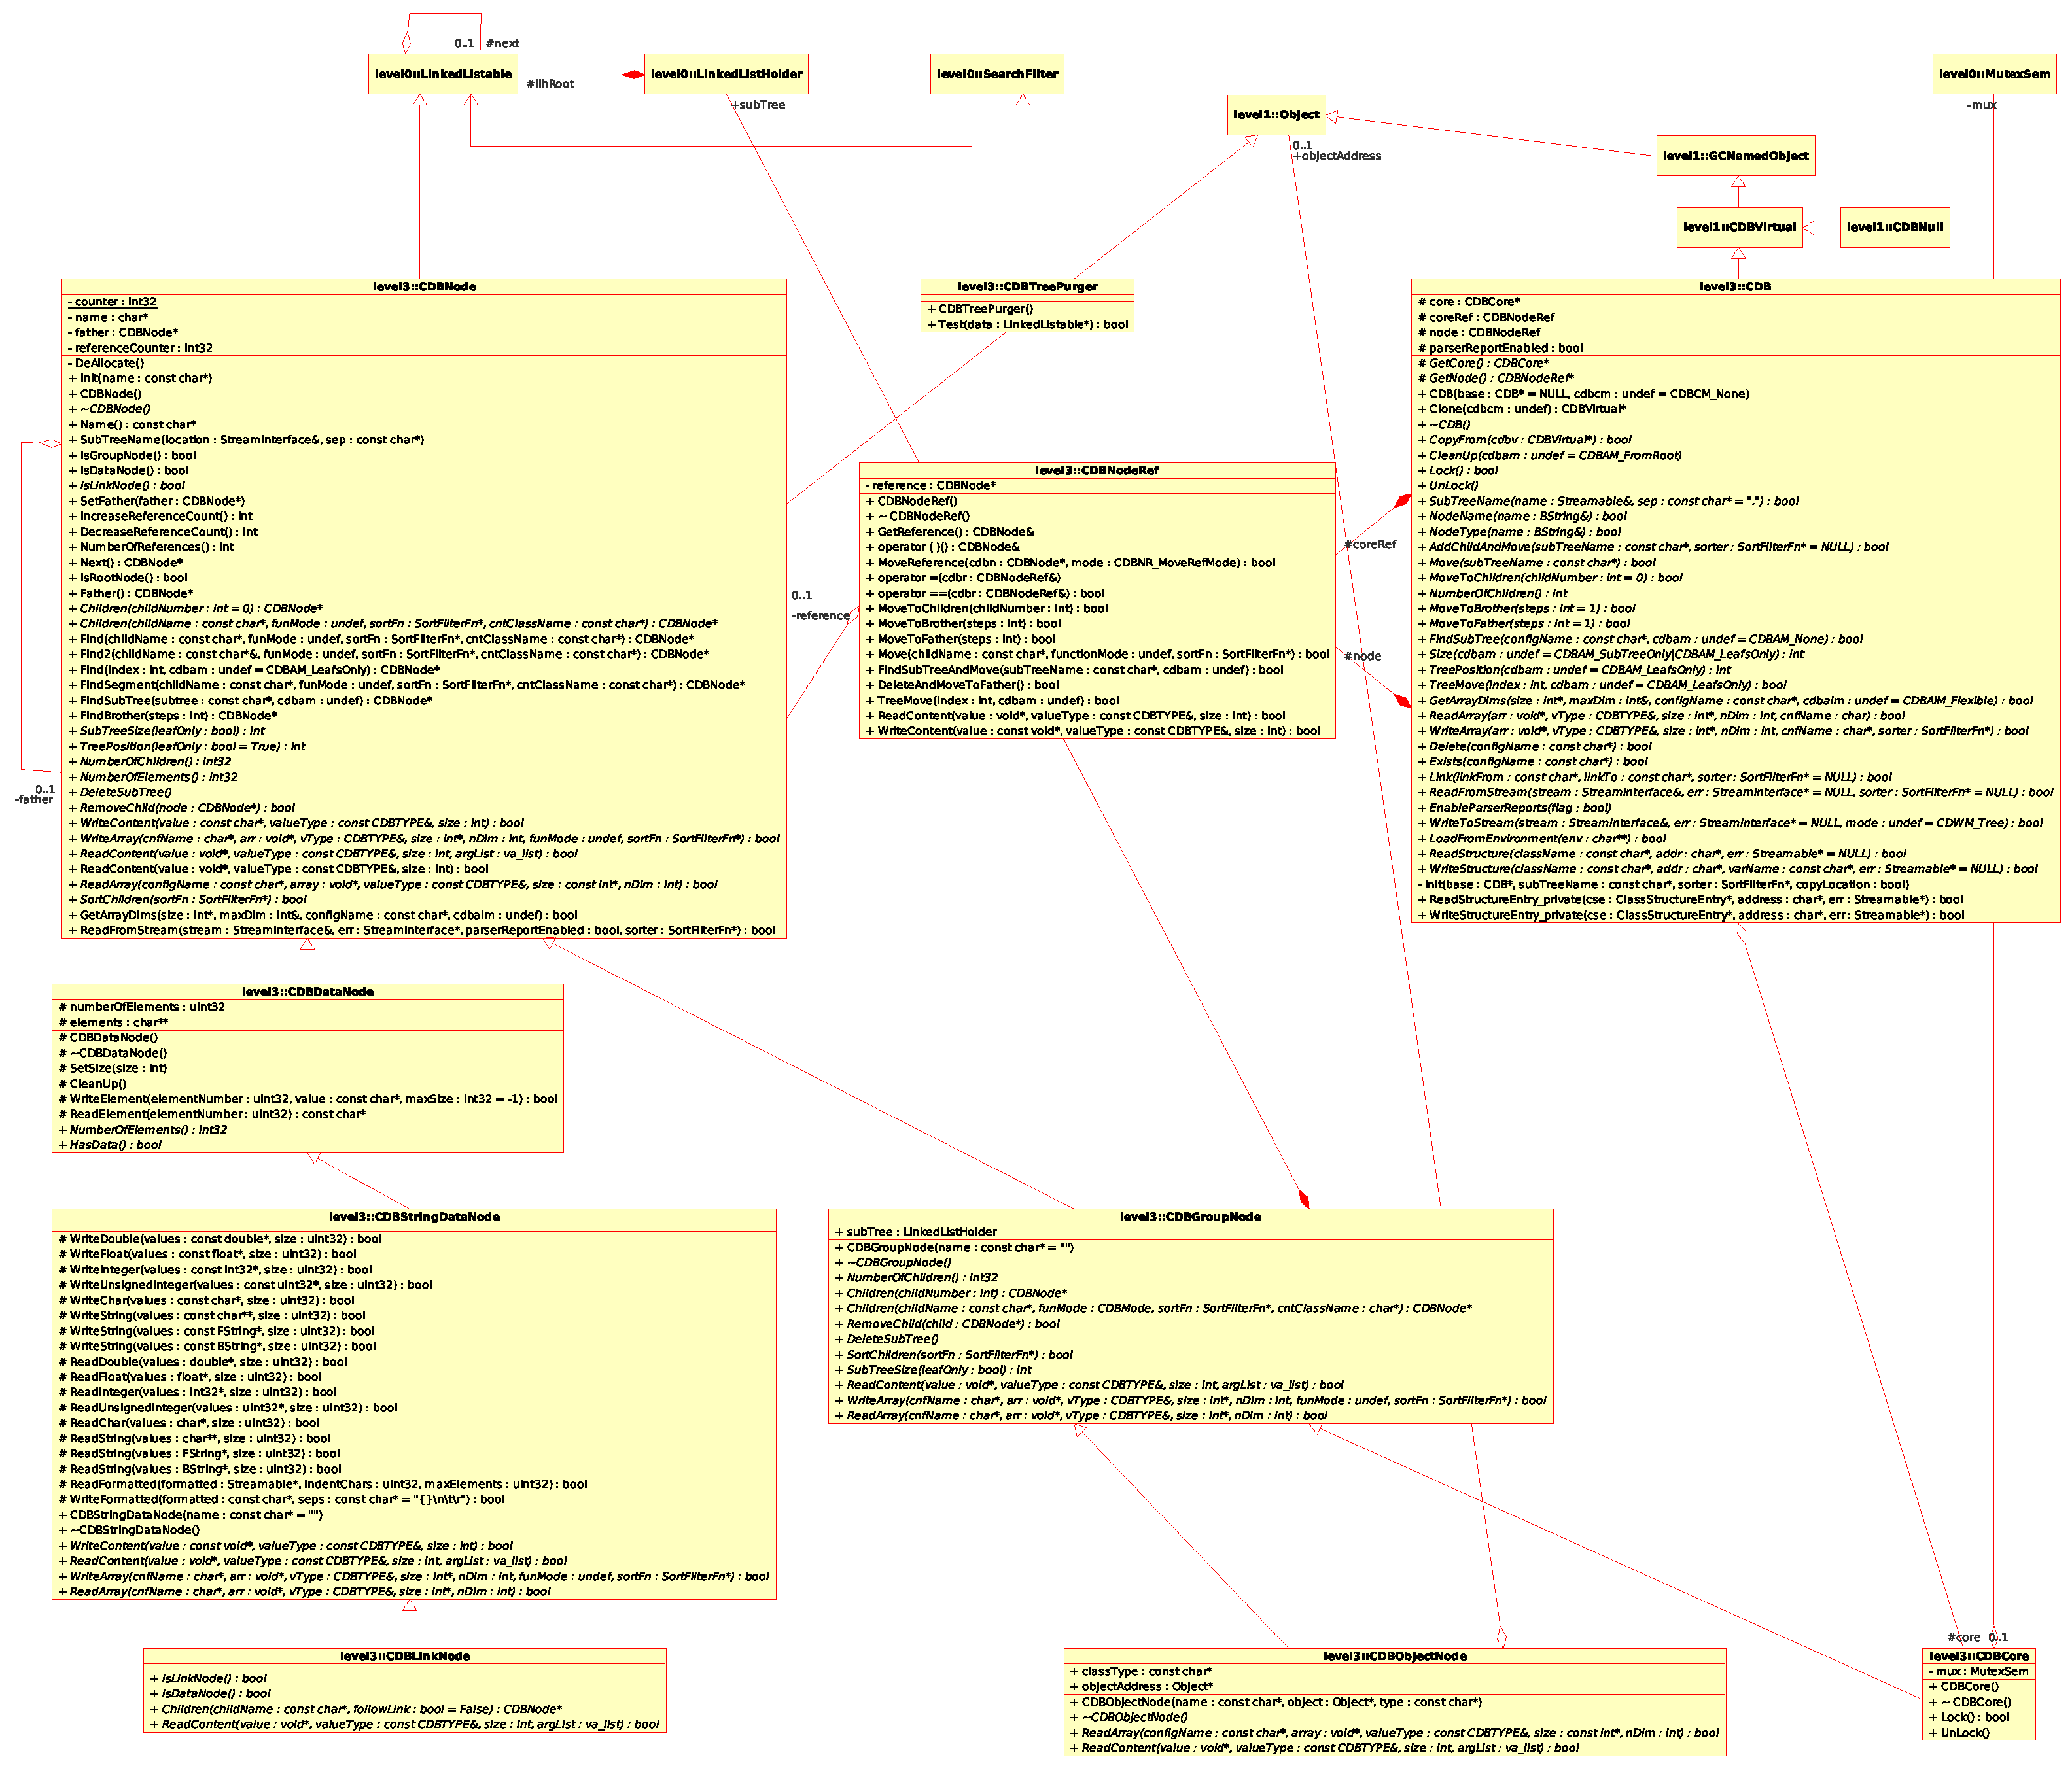
\includegraphics[width=1.1\textwidth]{level3/level3-CDB-exp.eps}
  \caption{BaseLib Level3 CDB (a Configuration Database implementation)}
  \label{f:level3:CDB-exp}
 \end{center}
\end{figure}

Class in this section are listed below.
\begin{itemize}
 \item CDBNode
 \item CDBDataNode
 \item CDBStringDataNode
 \item CDBLinkNode
 \item CDBGroupNode
 \item CDBObjectNode
 \item CDBCore
 \item CDBNodeRef
 \item CDB
 \item CDBCInterface
 \item CDBTreePurger
 \item CDBDataTypeInterface
\end{itemize}

The CDB tree data structure is designed with two basic data structures: leafs and internal nodes. Each internal node has at least a leaf (or another internal node). An internal node is a \texttt{CDBroupNode} and a leaf is a \texttt{CDBDataNode}. Figure \ref{f:level3:cdb-tree} depicts the structure described.

\begin{figure}[h!]
 \begin{center}
  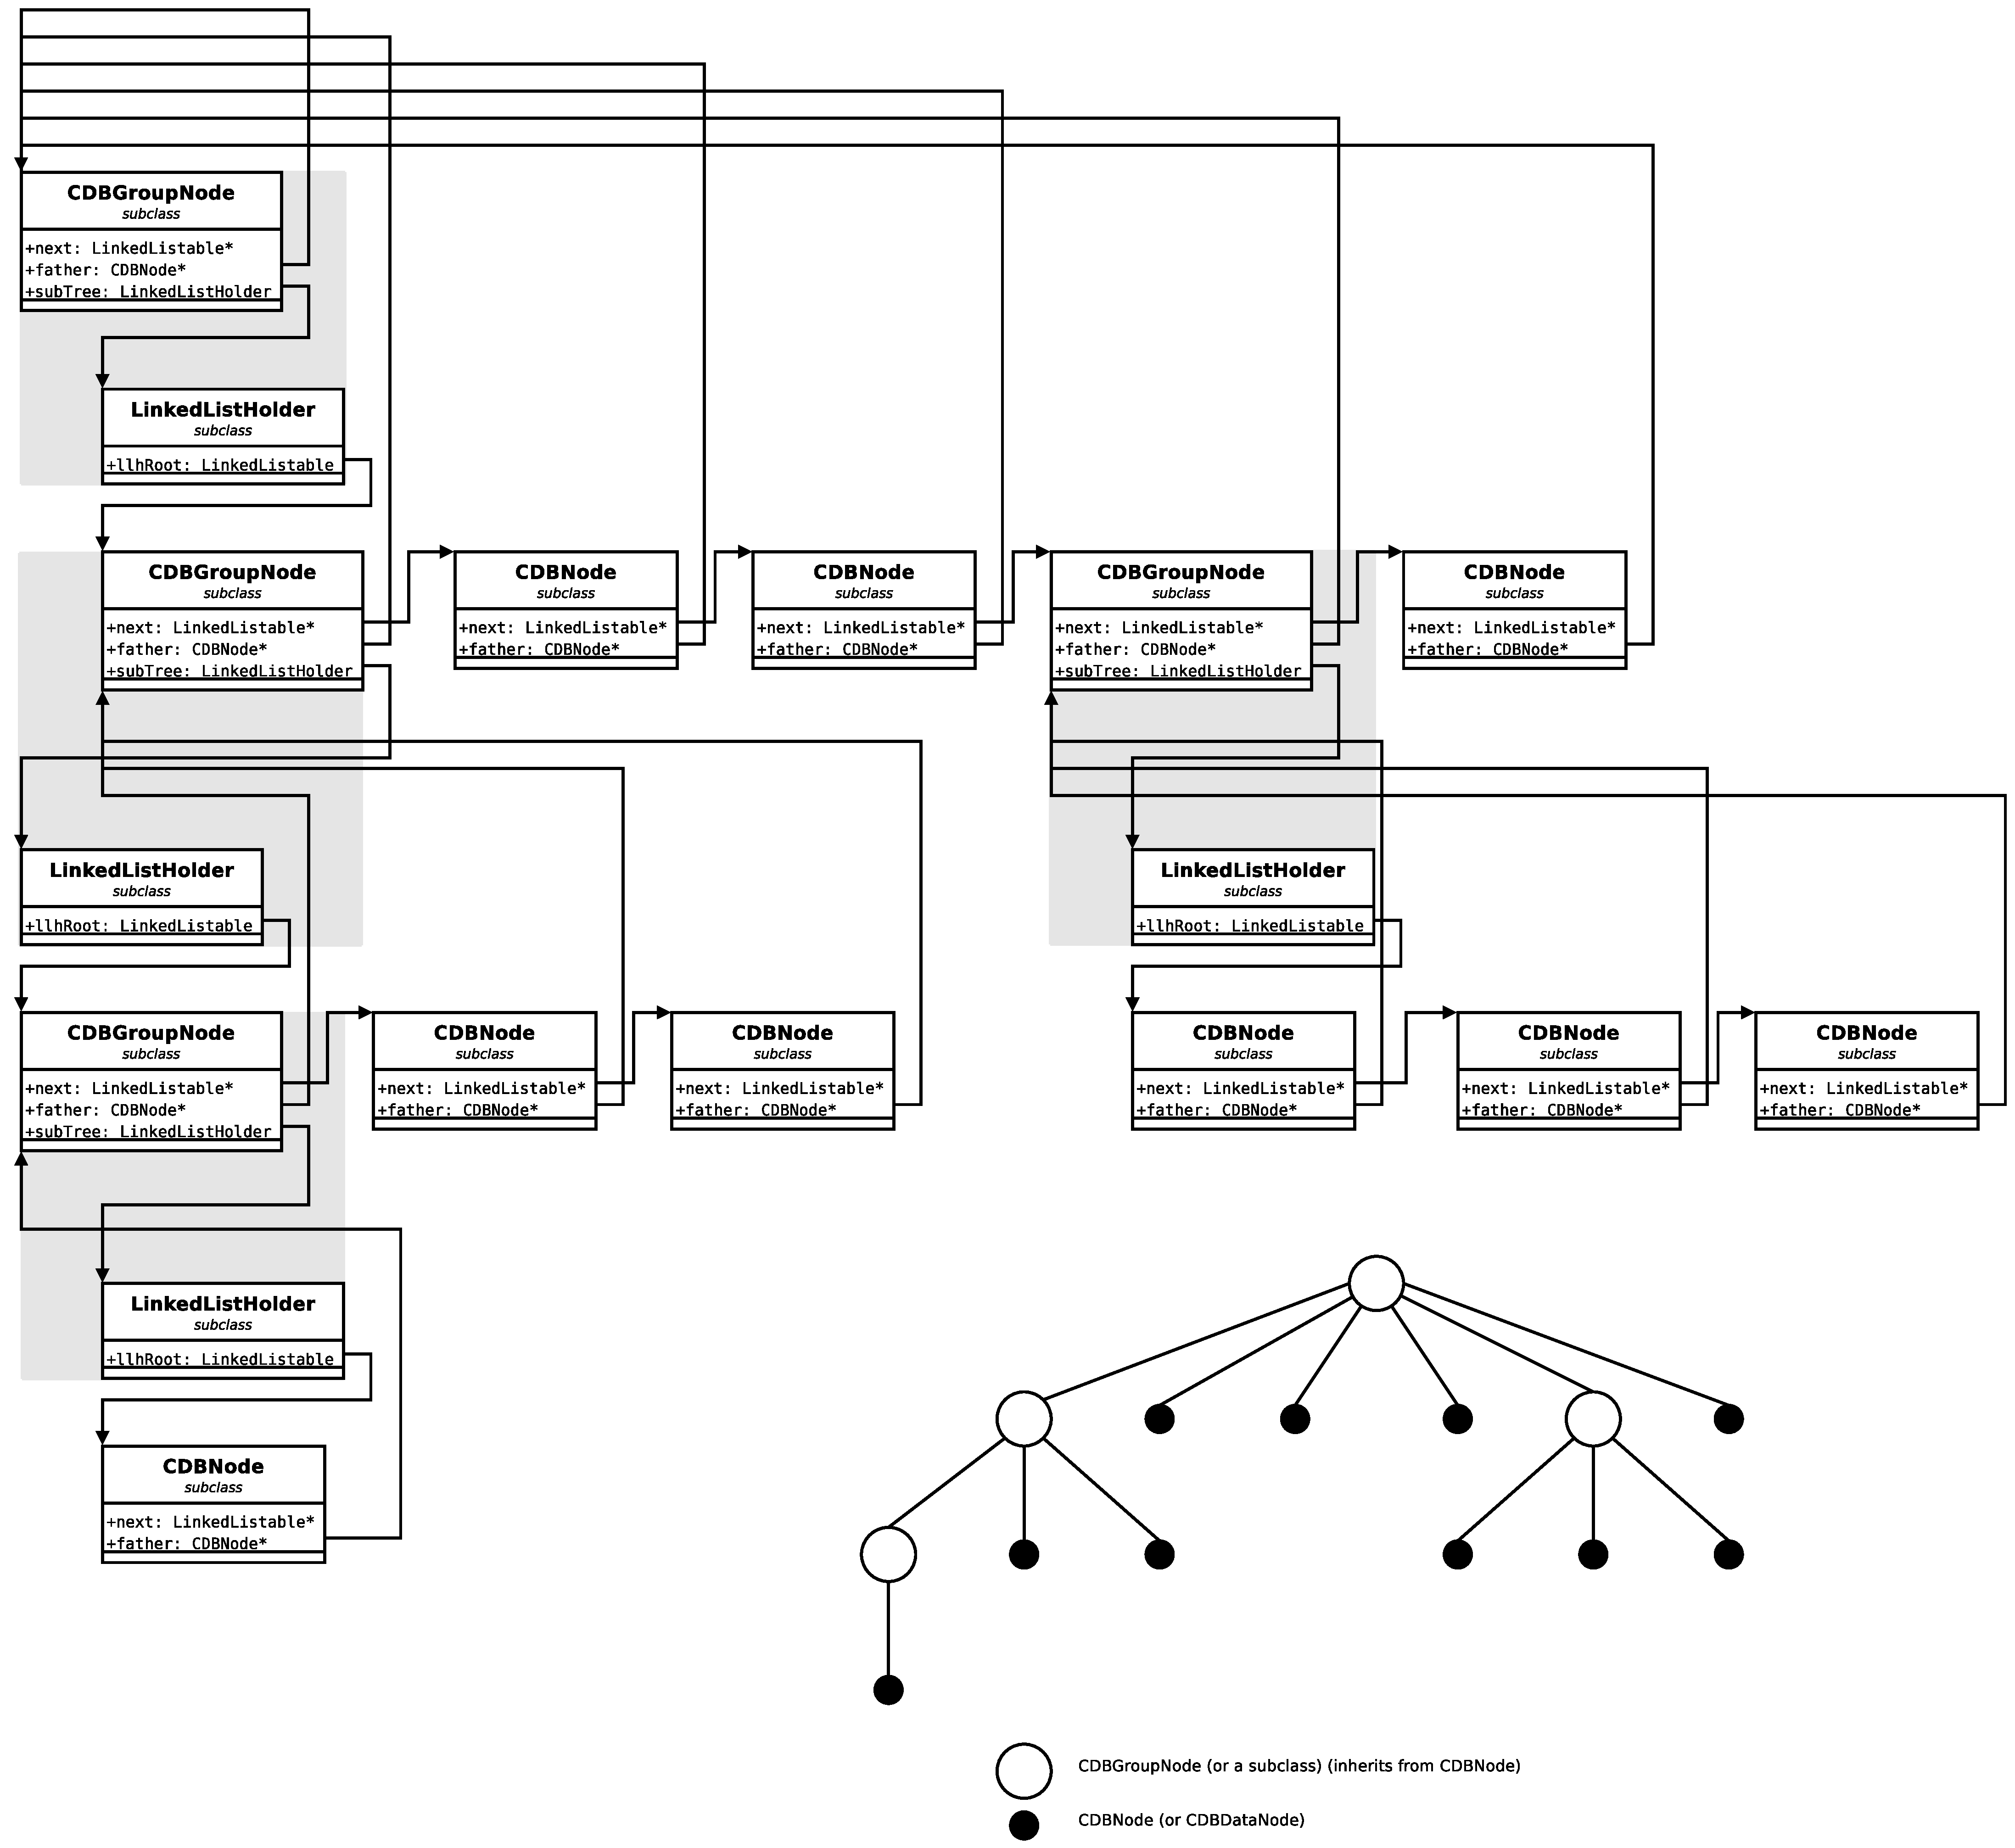
\includegraphics[width=\textwidth]{level3/CDB.eps}
  \caption{BaseLib Level3 CDB tree implementation}
  \label{f:level3:cdb-tree}
 \end{center}
\end{figure}



\subsubsection{CDBNode}
\texttt{[CDBNode.h, CDBNode.cpp]}\\
The class \texttt{CDBNode} is the basic node interface of the CDB tree data structure. Each type of node is build up the \texttt{CDBNode} class. In Figure \ref{f:level3:cdb-tree} the tree data structure of a CDB is depicted, each class is a \texttt{CDBNode} or a derived class of a \texttt{CDBNode}, class \texttt{level0::LinkedListHolder} is necessary to hold a linked list of \texttt{CDBNode} objects (of type \texttt{LinkedListable}).\\


We now switch to speak about attributes and methods of the \texttt{CDBNode} class. A \texttt{CDBNode} as the first attribute has a \texttt{static} \texttt{counter}, this variable lets hold the total number of nodes there are in the system, i.e. in the CDB, the constructor increment it and the deconstructor decrement it. Every node has a \texttt{name} that is really the name of the field, an object that it is its \texttt{father} in the tree and a \texttt{referenceCounter}, each node has its own \texttt{referenceCounter} for coherent destruction.
\begin{lstlisting}[
extendedchars=true,%
basicstyle=\fontfamily{pcr}\fontseries{m}\selectfont\footnotesize, %
stepnumber=1,%
numberstyle=\tiny,%
keywordstyle=\footnotesize\tt ,%
language=C++]
private:
   static int32 counter;

   char* name;
   CDBNode* father;
   int32 referenceCounter;
\end{lstlisting}

The first method we analysed is the private \texttt{DeAllocate} it deallocates memory used in a node (\texttt{name} allocated buffer); \texttt{Init} is public and inits the node and adds a name to it, then came the constructor and the destructor, that removes the node from its container also. \\


The method \texttt{Name} gets the \texttt{name} attribute of the class and \texttt{NumberOfElements} returns \texttt{-1} because such function must return how much data elements are contained by this node but a \texttt{CDBNode} is an abstraction of two node types so if is a leaf doesn't have elements but if it is an internal node it must have it. In this case it returns \texttt{-1} as an error, this function must be implemented at subclasses level. \\


The method \texttt{IsRootNode} check if the node is the root node of the tree, i.e. is a root node if the \texttt{father} attribute points to itself (is the same as the \texttt{this} pointer).
The method \texttt{IsGroupNode} in this case return \texttt{false} bacause only the subclass \texttt{CDBGroupNode} and derived return \texttt{true}; method \texttt{IsDataNode} returns \texttt{false} because \texttt{CDBNode} is not a \texttt{CDBDataNode} or a subclass of it. The methods \texttt{IsLinkNode()} return \texttt{true} whether it is a link to a different subtree, in the case of a \texttt{CDBNode} simply return \texttt{false}. \\


Methods \texttt{IncreaseReferenceCount}, \texttt{DecreaseReferenceCount} and \texttt{NumberOfReferences} increment, decrement and return atomically the attribute \texttt{referenceCounter}, such attribute show the number of users of this node. 
The method \texttt{Next} gets the next node, method \texttt{Father} gets the father of the node that you can sets via the method \texttt{SetFather}.
\begin{lstlisting}[
extendedchars=true,%
basicstyle=\fontfamily{pcr}\fontseries{m}\selectfont\footnotesize, %
stepnumber=1,%
numberstyle=\tiny,%
keywordstyle=\footnotesize\tt ,%
language=C++]
   void DeAllocate();
public:
   void Init(const char* name);

   CDBNode();
   virtual ~CDBNode();

   const char* Name() const;
   virtual int32 NumberOfElements() const;

   bool IsRootNode() const;
   inline bool IsGroupNode() const;
   inline bool IsDataNode() const;
   virtual bool IsLinkNode() const;

   int IncreaseReferenceCount();
   int DecreaseReferenceCount();
   int NumberOfReferences() const;

   CDBNode* Next() const;
   CDBNode* Father() const;
   void SetFather(CDBNode* father);
\end{lstlisting}

The first \texttt{Find} method finds a location within the whole (sub)tree as the object invoked on; remember that nodes are nombered from left to right and from subnode to supernode, if the node does not exist returns \texttt{false} and remains in the start position.

The second \texttt{Find} method simply call \texttt{Find2} method that has a sligtly different argument signature. \texttt{Find2} moves recursively in the tree from current position; \texttt{childName} can also be ``UpNode'' if you search is one level up, or ``RootNode'' if it is all the way up. Any movement onto unexisting subtree will fail; any movement out of unexisting subtree will erase temporary holders; movement is relative to current location. \texttt{childName} is returned modified to reflect the depth of matching.

The method \texttt{FindSegment} moves one level in the tree, we must remember that the CDB is a configuration tree that holds configuration data, as \texttt{Find2} \texttt{childName} argument if ``UpNode'' means one level up and if means ``RootNode'' is all the way up; as before any movement onto unexisting subtree will fail,any movement out of unexisting subtree will erase temporary holders; movement is relative to current location.
The method \texttt{FindSubTree}  moves to a node pointing to the specified subtree. \texttt{FindBrother} allows accessing brothers; negative and positive numbers allow to move relative to start position. \\


The method \texttt{SubTreeName} returns the name of the subtree starting from this node, this call is safe, does not require locking of tree. \texttt{SubTreeSize} returns \texttt{1} for a \texttt{CDBNode}, subclass of such class returns different values. \texttt{DeleteSubTree} will remove all unreferenced subtrees, in \texttt{CDBNode} doesn't take any action. \texttt{TreePosition} returns the position of the node within the tree. \\


The method \texttt{NumberOfChildren} returns how many childrens of this node, \texttt{-1} means it is not a node that has children, in this implementation \texttt{CDBNode} returns \texttt{-1}. The first \texttt{Children} allows accessing the subtrees and uptrees (using negative indexes -1 -2), \texttt{CDBNode} implements only access to uptrees. Second \texttt{Children} method allows accessing the subtrees by name, \texttt{childName} is the name of the node, it cannot be a full subtree; \texttt{functionMode} is of type \texttt{CDBNMode}, argument \texttt{sortFn} is used only if adding a node; this method is not implemented in \texttt{CDBNode} and simply return \texttt{NULL}. \texttt{SortChildren} apply sorting to the subtree; \texttt{RemoveChild} removes the specified child if exists.
\begin{lstlisting}[
extendedchars=true,%
basicstyle=\fontfamily{pcr}\fontseries{m}\selectfont\footnotesize, %
stepnumber=1,%
numberstyle=\tiny,%
keywordstyle=\footnotesize\tt ,%
language=C++]
   CDBNode* Find(int index,CDBAddressMode cdbam=CDBAM_LeafsOnly);
   inline CDBNode* Find(const char* childName,CDBNMode functionMode=CDBN_None,
      SortFilterFn* sortFn=NULL,const char* containerClassName=NULL);
   CDBNode* Find2(const char*& childName,CDBNMode functionMode=CDBN_None,
      SortFilterFn* sortFn=NULL,const char* containerClassName=NULL);
   CDBNode* FindSegment(const char* childName,CDBNMode functionMode=CDBN_None,
      SortFilterFn* sortFn=NULL,const char* containerClassName=NULL);
   CDBNode* FindSubTree(const char* subtree,CDBAddressMode cdbam);
   CDBNode* FindBrother(int steps);

   void SubTreeName(Streamable& location, const char* sep);
   virtual int SubTreeSize(bool leafOnly);
   virtual void DeleteSubTree();
   virtual int TreePosition(bool leafOnly = True);

   virtual int32 NumberOfChildren() const;
   virtual CDBNode* Children(int childNumber=0);
   virtual CDBNode* Children(const char* childName,CDBNMode functionMode=CDBN_SearchOnly,
      SortFilterFn* sortFn=NULL,const char* containerClassName=NULL);
   virtual bool SortChildren(SortFilterFn* sortFn);
   virtual bool RemoveChild(CDBNode* node);
\end{lstlisting}

Methods \texttt{WriteContent}, \texttt{WriteArray}, \texttt{ReadContent} and \texttt{ReadArray} are all implemented in subclasses and in the class \texttt{CDBNode} simply return \texttt{false}. Read and write methods are implemented in \texttt{CDBDataNode} and subclasses.\\


The method \texttt{GetArrayDim} reads the dimensions of a matrix, it expects all the indexes to be found form $0$ to $N$. \texttt{ReadFromStream} parses the stream and build a configuration database according to the simple CDB syntax. Those methods are implemented in \texttt{CDBNode}.
\begin{lstlisting}[
extendedchars=true,%
basicstyle=\fontfamily{pcr}\fontseries{m}\selectfont\footnotesize, %
stepnumber=1,%
numberstyle=\tiny,%
keywordstyle=\footnotesize\tt ,%
language=C++]
   virtual bool WriteContent(const void* value,const CDBTYPE& valueType,int size);
   virtual bool WriteArray(const char* configName,const void* array,
      const CDBTYPE& valueType,const int* size,int nDim,
      CDBNMode functionMode=CDBN_CreateStringNode,SortFilterFn* sortFn=NULL);

   virtual bool ReadContent(void* value,const CDBTYPE& valueType,
      int size,va_list argList);
   bool ReadContent(void* value,const CDBTYPE& valueType,int size,...);
   virtual bool ReadArray(const char* configName,void* array,
      const CDBTYPE& valueType,const int* size,int nDim);

   bool GetArrayDims(int* size,int& maxDim,const char* configName,
      CDBArrayIndexingMode cdbaim);
   bool ReadFromStream(StreamInterface& stream,StreamInterface* err,
      bool parserReportEnabled,SortFilterFn* sorter);
\end{lstlisting}



\subsubsection{CDBDataNode}
\texttt{[CDBStringDataNode.h, CDBStringDataNode.cpp]}\\
The class \texttt{CDBDataNode} is the low level abstraction of all nodes containing data. It basically adds few methods and ttributes to the \texttt{CDBNode} class. \\


The first attribute \texttt{numberOfElements} can be $1$ if the other attribute, \texttt{elements}, points to a string directly; greater then $1$ if \texttt{elements} is a pointer to an array of pointers.
As we said \texttt{elements} is a vector of pointers or a direct pointer to data if \texttt{numberOfElements} is $1$, if \texttt{numberOfElements} is $0$ \texttt{elements} should be \texttt{NULL}. \\


Constructor set \texttt{elements} to \texttt{NULL} and \texttt{numberOfElements} to $0$; deconstructor call the method \texttt{CleanUp}.

The method \texttt{SetSize} resize data structure, i.e. it will call malloc on the attribute \texttt{elements} and copies the old data. \texttt{CleanUp} frees each elements and turn the data structure to $0$ elemnts like the constructor.

The method \texttt{WriteElement} adds a new element in the \texttt{elements} array, such function handle also allocation of the memory, with the \texttt{ReadElement} method is also possible to read the entry just written.

The method \texttt{NumberOfElements} simply return the attribute \texttt{NumberOfElements}, i.e. how much data elements are contained by this node, $-1$ means it is not a node that has data. \texttt{HasData} return \texttt{true} whether it is to be considered a leaf node.
\begin{lstlisting}[
extendedchars=true,%
basicstyle=\fontfamily{pcr}\fontseries{m}\selectfont\footnotesize, %
stepnumber=1,%
numberstyle=\tiny,%
keywordstyle=\footnotesize\tt ,%
language=C++]
protected:
   uint32 numberOfElements;
   char** elements;

   CDBDataNode();
   ~CDBDataNode();

   void SetSize(int size);
   void CleanUp();
   bool WriteElement(uint32 elementNumber,const char* value,int32 maxSize=-1);
   const char* ReadElement(uint32 elementNumber) const;

   virtual int32 NumberOfElements() const;
   virtual bool HasData() const;
\end{lstlisting}



\subsubsection{CDBStringDataNode}
\texttt{[CDBStringDataNode.h, CDBStringDataNode.cpp]}\\
The class \texttt{CDBStringDataNode} is a csubclass of a \texttt{CDBDataNode} that holds data in string format, it is possible to convert from a string to each other type. Obviously if a string is a character array of letters can't be converted in a double. The class provides no attributes. \\


Following methods write (it makes a copy) of respectively double, float, integer, unsigned integer, char and strings from the first argument to the \texttt{CDBDataNode::elements} pointer. Each method accept in input not only one value but an array of data with the same format. Read methods have the same behaviour but copy the \texttt{elements} pointer to the \texttt{values} argument.
All the write methods make use of the superclass method's \texttt{CDBDataNode::WriteElement} and write methods of \texttt{CDBDataNode::ReadElement}.
\begin{lstlisting}[
extendedchars=true,%
basicstyle=\fontfamily{pcr}\fontseries{m}\selectfont\footnotesize, %
stepnumber=1,%
numberstyle=\tiny,%
keywordstyle=\footnotesize\tt ,%
language=C++]
protected:
   bool WriteDouble(const double* values,uint32 size);
   bool WriteFloat(const float* values,uint32 size);
   bool WriteInteger(Const int32* values,uint32 size);
   bool WriteUnsignedInteger(const uint32* values,uint32 size);
   bool WriteChar(const char* values,uint32 size);
   bool WriteString(const char** values,uint32 size);
   bool WriteString(const FString* values,uint32 size);
   bool WriteString(const BString* values,uint32 size);

   bool ReadDouble(double* values,uint32 size);
   bool ReadFloat(float* values,uint32 size);
   bool ReadInteger(int32* values,uint32 size);
   bool ReadUnsignedInteger(uint32* values,uint32 size);
   bool ReadChar(char* values,uint32 size);
   bool ReadString(char** values,uint32 size);
   bool ReadString(FString* values,uint32 size);
   bool ReadString(BString* values,uint32 size);
\end{lstlisting}

The method \texttt{WriteFormatted} takes a formatted string as an input and write it in the texttt{CDBDataNode::elements} attribute; probably the formatted input can contain data of different type. The method \texttt{ReadFormatted} read outputting on the \texttt{Streamable} argument all the elements in the \texttt{CDBDataNode} array, inserting ${}$ around the formatted stream.
\begin{lstlisting}[
extendedchars=true,%
basicstyle=\fontfamily{pcr}\fontseries{m}\selectfont\footnotesize, %
stepnumber=1,%
numberstyle=\tiny,%
keywordstyle=\footnotesize\tt ,%
language=C++]
   bool WriteFormatted(const char* formatted,const char* seps=" {}\n\t\r");
   bool ReadFormatted(Streamable* formatted,uint32 indentChars,uint32 maxElements);
\end{lstlisting}

Now comes public methods. The method \texttt{WriteContent} writes data on a node the value can be of any \texttt{CDBTYPE} the \texttt{size} argument specifies how many elements. The class \texttt{CDBTYPE} is declared in \textit{level1}. Table shows registered \texttt{CDBTYPE}s, from \textit{level1/CDBTypes.h}.

\begin{table}[!h]
 \begin{center}
  \begin{tabular}{|l|l|l|}
   \hline
name & CDBDataType & sizeof() \\
    \hline
\texttt{CDBTYPE\_float} & \texttt{CDB\_float} & \texttt{float} \\
\texttt{CDBTYPE\_double} & \texttt{CDB\_double} & \texttt{double} \\
\texttt{CDBTYPE\_int32} & \texttt{CDB\_int32} & \texttt{int32} \\
\texttt{CDBTYPE\_uint32} & \texttt{CDB\_uint32} & uint32 \\
\texttt{CDBTYPE\_char} & \texttt{CDB\_char} & \texttt{char} \\
\texttt{CDBTYPE\_hex} & \texttt{CDB\_hex} & \texttt{uint32} \\
\texttt{CDBTYPE\_octal} & \texttt{CDB\_octal} & \texttt{uint32} \\
\texttt{CDBTYPE\_String} & \texttt{CDB\_String} & \texttt{char*} \\
\texttt{CDBTYPE\_BString} & \texttt{CDB\_BString} & \texttt{BString} \\
\texttt{CDBTYPE\_NULL} & \texttt{CDB\_None} & \texttt{NULL} \\
    \hline
    \end{tabular}
   \end{center}
  \caption{Level1 declared \texttt{CDBTYPE}s in \textit{level1/CDBTypes.h} }
 \label{t:level1:CDBTYPE}
\end{table}

\texttt{ReadContent} reads data from a node, \texttt{valueType} specifies data type, \texttt{size} specifies how many elements and \texttt{value} contains a pointer to memory where to write the data.

The method \texttt{WriteArray} writes content (one to many elements) into a data node, creates a data node or modifies an existing, \texttt{configName} is the address of the parameter relative to the current node, \texttt{array} is the data in whatever form specified by \texttt{valueType} and \texttt{size} is a vector of matrix dimensions; if \texttt{size} is \texttt{NULL} it treats the input as a monodimensional array of size \texttt{nDim}; \texttt{sortFn} allows inserting newly created nodes in a specific order.
The method \texttt{ReadArray} reads content from a data node to the \texttt{configName} pointer argument.
\begin{lstlisting}[
extendedchars=true,%
basicstyle=\fontfamily{pcr}\fontseries{m}\selectfont\footnotesize, %
stepnumber=1,%
numberstyle=\tiny,%
keywordstyle=\footnotesize\tt ,%
language=C++]
public:
   CDBStringDataNode(const char* name="");
   ~CDBStringDataNode();

   virtual bool WriteContent(const void* value,const CDBTYPE& valueType,int size);
   virtual bool ReadContent(void* value,const CDBTYPE& valueType,int size,va_list argList);

   virtual bool WriteArray(const char* configName,const void* array,
      const CDBTYPE& valueType,const int* size,int nDim,
      CDBNMode functionMode=CDBN_CreateStringNode,SortFilterFn* sortFn=NULL);
   virtual bool ReadArray(const char* configName,void* array,
      const CDBTYPE& valueType,const int* size,int nDim);
\end{lstlisting}



\subsubsection{CDBLinkNode}
\texttt{[CDBLinkNode.h, CDBLinkNode.cpp]}\\
Such \texttt{CDBLinkNode} should implements hard link between nodes. The constructor calls the superclass constructor, this class is a subclass of a \texttt{CDBStringDataNode}. \\


Methods \texttt{IsLinkNode} and \texttt{IsDataNode} return \texttt{true} each.
\texttt{Children} allows accessing the subtrees by name but in this case simply return \texttt{NULL}; if argument \texttt{followLink} is \texttt{true} links are followed.
\texttt{ReadContent} reads data from a node, this is the only real method implemented, it should find what to read in the \texttt{value} argument and then treat the same argument as an output stream. Not really well implemented.
\begin{lstlisting}[
extendedchars=true,%
basicstyle=\fontfamily{pcr}\fontseries{m}\selectfont\footnotesize, %
stepnumber=1,%
numberstyle=\tiny,%
keywordstyle=\footnotesize\tt ,%
language=C++]
public:
   CDBLinkNode(const char *name);
   virtual bool IsLinkNode() const;
   virtual bool IsDataNode() const;
   virtual CDBNode* Children(const char* childName,bool followLink=False);
   virtual bool ReadContent(void* value,const CDBTYPE& valueType,int size,va_list argList);
\end{lstlisting}



\subsubsection{CDBGroupNode}
\texttt{[CDBGroupNode.h, CDBGroupNode.cpp]}\\
A CDB tree is constituited of two basic types of nodes: \texttt{CDBDataNode} and \texttt{CDBGroupNode} respectively leafs and internal nodes. Internal nodes are \texttt{CDBGroupNode} and basically are containers of \texttt{CDBNode}s, i.e. the branches of the tree. So the only, but the most important, attribute of this class is \texttt{subTree} a \texttt{LinkedListHolder} that holds all the nodes underneath in the tree.
\begin{lstlisting}[
extendedchars=true,%
basicstyle=\fontfamily{pcr}\fontseries{m}\selectfont\footnotesize, %
stepnumber=1,%
numberstyle=\tiny,%
keywordstyle=\footnotesize\tt ,%
language=C++]
public:
   LinkedListHolder subTree;
\end{lstlisting}

The constructor invokes the superclass's constructor with the passed by name; destructor call \texttt{LinkedListHolder::Reset} method. \texttt{NumberOfChildren} returns the number of elements contained in the linked list of the attribute, i.e. the number of children of this node.
The first \texttt{Children} method allows accessing the subtrees and uptrees (with negative values, -1 -2...),the links are not expanded by this function; second \texttt{Children} method allows accessing the subtrees by name, \texttt{childName} is the name of the node, it cannot be a full subtree; \texttt{followLink} if \texttt{true} links are followed, \texttt{sortFn} used only if adding a node.
The method \texttt{RemoveChild} removes a child by name; \texttt{DeleteSubTree} removes all unreferenced subtrees; \texttt{SortChildren} apply sorting. \texttt{SubTreeSize} returns how many elements in the sub tree, note that is far different from \texttt{NumberOfChildren} because counts elements in all the sub tree from the node.
\begin{lstlisting}[
extendedchars=true,%
basicstyle=\fontfamily{pcr}\fontseries{m}\selectfont\footnotesize, %
stepnumber=1,%
numberstyle=\tiny,%
keywordstyle=\footnotesize\tt ,%
language=C++]
public:
   CDBGroupNode(const char* name="");
   virtual ~CDBGroupNode();

   virtual int32 NumberOfChildren() const;
   virtual CDBNode* Children(int childNumber);
   virtual CDBNode* Children(const char* childName,
      CDBNMode functionMode=CDBN_SearchOnly,SortFilterFn* sortFn=NULL,
      const char* containerClassName=NULL);
   virtual bool RemoveChild(CDBNode* child);
   virtual void DeleteSubTree();
   virtual bool SortChildren(SortFilterFn* sortFn);
   virtual int SubTreeSize(bool leafOnly);
\end{lstlisting}

Methods that follow are just be analysed before and are not treated here. All those three methods, \texttt{ReadContent}, \texttt{WriteArray} and \texttt{ReadArray} are implemented here.
\begin{lstlisting}[
extendedchars=true,%
basicstyle=\fontfamily{pcr}\fontseries{m}\selectfont\footnotesize, %
stepnumber=1,%
numberstyle=\tiny,%
keywordstyle=\footnotesize\tt ,%
language=C++]
   virtual bool ReadContent(void* value,const CDBTYPE& valueType,
      int size,va_list argList);

   virtual bool WriteArray(const char* configName,const void* array,
      const CDBTYPE& valueType,const int* size,int nDim,�
      CDBNMode functionMode=CDBN_CreateStringNode,SortFilterFn* sortFn=NULL);
   virtual bool ReadArray(const char* configName,void* array,
      const CDBTYPE& valueType,const int* size,int nDim);
\end{lstlisting}



\subsubsection{CDBObjectNode}
\texttt{[CDBObjectNode.h, CDBObjectNode.cpp]}\\
From the sources it is possible to read that a \texttt{CDBObjectNode} is ``a container of CDBNodes and of an Object''; most important is that the \texttt{CDBObjectNode} class inherits from \texttt{CDBGroupNode} and has as attributes a \texttt{const char*} and a \texttt{Object*} so it has an \texttt{Object} associated with it. The constructor register the name of the node, the pointer to the object and also the class type as a string.\\


The method \texttt{ReadArray} reads content from a data node, \texttt{configName} is the address of the parameter relative to the current node, \texttt{array} is the data in wahtever form specified by \texttt{valueType}, \texttt{size} is a vector of matrix dimensions, if \texttt{size} is \texttt{NULL} it treats the input as a monodimensional array of size \texttt{nDim}; \texttt{nDim} specifies how many dimensions the array possesses or the vector size if \texttt{size} is \texttt{NULL}. \texttt{ReadContent} reads also data from a node argument \texttt{value} contains a pointer to memory where to write the data.
\begin{lstlisting}[
extendedchars=true,%
basicstyle=\fontfamily{pcr}\fontseries{m}\selectfont\footnotesize, %
stepnumber=1,%
numberstyle=\tiny,%
keywordstyle=\footnotesize\tt ,%
language=C++]
public:
   const char* classType;
   Object* objectAddress;

   CDBObjectNode(const char* name,Object* object,const char* type);
   virtual ~CDBObjectNode();

   virtual bool ReadArray(const char* configName,void* array,
      const CDBTYPE& valueType,const int* size,int nDim);
   virtual bool ReadContent(void* value,const CDBTYPE& valueType,
      int size,va_list argList);
\end{lstlisting}



\subsubsection{CDBCore}
\texttt{[CDBCore.h]}\\
Probably the class \texttt{CDBCore} is the most simplest class of \textit{level3}, it only use a \texttt{level0:MutexSem} guaranteeing shared access to a CDB context safe. The class code follow.
\begin{lstlisting}[
extendedchars=true,%
basicstyle=\fontfamily{pcr}\fontseries{m}\selectfont\footnotesize, %
stepnumber=1,%
numberstyle=\tiny,%
keywordstyle=\footnotesize\tt ,%
language=C++]
class CDBCore: public CDBGroupNode{
private:
   MutexSem mux;
public:
   CDBCore(){ mux.Create();}
   virtual ~CDBCore(){ }
   virtual bool Lock(){
      if (!mux.Lock()){
         CStaticAssertErrorCondition(FatalError,"CDBCore Lock failed!");
         return False;
      }
      return True;
   }
   virtual void UnLock(){
      mux.UnLock();
   }
};
\end{lstlisting}



\subsubsection{CDBNodeRef}
\texttt{[CDBNodeRef.h, CDBNodeRef.cpp]}\\
The class \texttt{CDBNodeRef} is a reference to a \texttt{CDBNode} that remaps some methods. The only attribute is infact a \texttt{CDBNode*}. The class is a kind of iterator to move between nodes.

The constructor takes no arguments and initialize the object to a dummy \texttt{CDBNode} reference. The distructor move the reference away. There is also a copy operator overridden and a compare operator redefinition.
\begin{lstlisting}[
extendedchars=true,%
basicstyle=\fontfamily{pcr}\fontseries{m}\selectfont\footnotesize, %
stepnumber=1,%
numberstyle=\tiny,%
keywordstyle=\footnotesize\tt ,%
language=C++]
   CDBNode* reference;
public:
   CDBNodeRef();
   ~CDBNodeRef();

   inline CDBNode &GetReference();
   inline CDBNode &operator();
   inline void operator=(CDBNodeRef &cdbr);
   inline bool operator==(CDBNodeRef &cdbr);
\end{lstlisting}

The method \texttt{MoveReference} changes the reference to the node, if argument \texttt{cdbn} is \texttt{NULL} than it will refer to the globally allocated \texttt{nullCDBNode}.

The method \texttt{MoveToChildren} allows accessing the subtrees (argument \texttt{childNumber>=0}) and uptree (-1, -2, -3, ...); \texttt{MoveToBrother} allows accessing the brothers and \texttt{MoveToFather} allows acceesing brothers.

The method \texttt{Move} is the general method that allows accessing the subtrees and uptrees, like in \texttt{CDBNode} ``UpNode'' is one level up and ``RootNode'' is all the way up, any movement onto unexisting subtree will fail; any movement out of unexisting subtree will erase temporary holders; finally movements are relative to current location. \\


The method \texttt{FindSubTreeAndMove} moves to a node pointing to the specified subtree; \texttt{DeleteAndMoveToFather} remove current node and move up, the operation will complete only if the number of users is 0, the up movement will happen anyway. \texttt{TreeMove} moves to a location within the whole (sub)tree. \\


The method \texttt{ReadContent} reads data on a node, \texttt{valueType} specifies data type and \texttt{size} specifies how many elements; \texttt{WriteContent} writes data on a node argument \texttt{valueType} specifies data type and \texttt{size} specifies how many elements.

\begin{lstlisting}[
extendedchars=true,%
basicstyle=\fontfamily{pcr}\fontseries{m}\selectfont\footnotesize, %
stepnumber=1,%
numberstyle=\tiny,%
keywordstyle=\footnotesize\tt ,%
language=C++]
   bool MoveReference( CDBNode *cdbn, CDBNR_MoveRefMode mode);
   inline bool MoveToChildren(int childNumber=0);
   inline bool MoveToBrother(int steps = 1);
   inline bool MoveToFather(int steps = 1);
   inline bool Move(const char* childName,CDBNMode functionMode=CDBN_None,
      SortFilterFn* sortFn=NULL);

   inline bool FindSubTreeAndMove(const char* subTreeName,
      CDBAddressMode cdbam=CDBAM_None);
   inline bool DeleteAndMoveToFather();
   inline bool TreeMove(int index,CDBAddressMode cdbam=CDBAM_LeafsOnly);

   bool ReadContent(void* value,const CDBTYPE& valueType,int size,...);
   inline bool WriteContent(const void* value,const CDBTYPE& valueType,int size);
\end{lstlisting}



\subsubsection{CDB}
\texttt{[CDB.h, CDB.cpp]}\\
Like a \texttt{CDBNull} a \texttt{CDB} class extends a \texttt{CDBVirtual}. A \texttt{CDB} is an implementation of a hierarchical database. It works similarly to a filesystem having directory nodes (internal nodes or branches) and file nodes (leaves).

Each leaf node (\texttt{CDBDataNode}) is a container of a sequence of characters, both ASCII and not ASCII. \texttt{CDB} is infact a reference to an instance of the database. Copying \texttt{CDB}s does not duplicate the database but increases a reference counter. Operation to the same database by different
threads is safe. \\


We start with the attributes as usual. The first attribute is a \texttt{CDBCore*} that is used to acquire concurrent access to a \texttt{CDB}, the first \texttt{CDBNodeRef} is a pointer to the root node of the \textit{Configuration DataBase}, second \texttt{CDBNodeRef} is a pointer to the current node, obviously it can point to branches or leaves. Last argument \texttt{parserReportEnabled} said whether parsing reports faults.

The method \texttt{GetCore} basically return the \texttt{core} attribute and \texttt{GetNode} return a reference to the \texttt{node} attribute.
\begin{lstlisting}[
extendedchars=true,%
basicstyle=\fontfamily{pcr}\fontseries{m}\selectfont\footnotesize, %
stepnumber=1,%
numberstyle=\tiny,%
keywordstyle=\footnotesize\tt ,%
language=C++]
protected:
   CDBCore* core;
   CDBNodeRef coreRef;
   CDBNodeRef node;
   bool parserReportEnabled;

   virtual CDBCore* GetCore();
   virtual CDBNodeRef* GetNode();
\end{lstlisting}

The first method is the constructor of a CDB, if \texttt{base} is specified it creates a new reference to an existing database; if \texttt{NULL} creates a new database; argument \texttt{cdbcm} must be \texttt{CDBCM\_CopyAddress} to copy the address from the reference; in case of two or more flags, after oring one must cast back to the enum type. \texttt{Clone} simply call the constructor with \texttt{this } as \texttt{base} argument creating a new reference to a database, or if that is not possible it creates a copy. Then comes the destructor that does nothing, but will destroy database if instance count goes to zero. The method \texttt{CopyFrom} copy all the \texttt{CDB} passed by to the current \texttt{CDB}. \texttt{CleanUp} removes all the content from the database unless some other database instance exists and points to a subtree one can request to delete only the current subtree. \\


The method \texttt{Lock} locks the main database for exclusive access: use if a group of transactions should be atomic, \texttt{UnLock} unlocks the main database: remember unlocking a locked database after use. \\


The method \texttt{SubTreeName} finds the overall path leading to the current node, \texttt{NodeName} returns the name of the current node and \texttt{NodeType} gets the type of the current node. \\


The method \texttt{AddChildAndMove} can be used to create a new subtree, \texttt{Move} moves the \texttt{node} attribute to the specified location, the movement is relative to the current location. \texttt{MoveToChildren} moves the \texttt{node} attribute, negative number move up, zero is the first of the children; \texttt{NumberOfChildren} returns how many branches there are from this node; negative number implies that the location is a leaf. The method \texttt{MoveToBrother} moves to a brother's node, with $0$ means remain where you are, greater then $0$ brothers on the right below $0$ on the left.
\texttt{MoveToFather} moves up, \texttt{-1} means \texttt{Root}, one level up for each positive. \\


The method \texttt{FindSubTree} search a node identified by \texttt{configName} attribtue from node search on the right of the tree for the subtree identified by the string name, on success \texttt{node} attribute points to the node containing the subtree or leaf, such method will not follow links.
\texttt{Size} return the total number of nodes, param \texttt{cdbam} if \texttt{CDBAM\_SubTreeOnly} allows to measure the current subtree and if is \texttt{CDBAM\_LeafsOnly} allows counting only the data nodes.
The method \texttt{TreePosition} return the absolute location of a node in the tree in left to right bottom to top order. \texttt{TreeMove} moves to a location within the whole (sub)tree; nodes are numbered from left to right and from subnode to supernode; if the node does not exist returns \texttt{False} and remains in the start position.
\begin{lstlisting}[
extendedchars=true,%
basicstyle=\fontfamily{pcr}\fontseries{m}\selectfont\footnotesize, %
stepnumber=1,%
numberstyle=\tiny,%
keywordstyle=\footnotesize\tt ,%
language=C++]
public:
   CDB(CDB* base=NULL,CDBCreationMode cdbcm=CDBCM_None);
   CDBVirtual* Clone(CDBCreationMode cdbcm);
   virtual ~CDB();
   virtual bool CopyFrom(CDBVirtual* cdbv);
   virtual void CleanUp(CDBAddressMode cdbam=CDBAM_FromRoot);

   virtual bool Lock();
   virtual void UnLock();

   virtual bool SubTreeName(Streamable& name,const char* sep=".");
   virtual bool NodeName(BString& name);
   virtual bool NodeType(BString& name);

   virtual bool AddChildAndMove(const char* subTreeName,SortFilterFn* sorter=NULL);
   virtual bool Move(const char* subTreeName);
   virtual bool MoveToChildren(int childNumber=0);
   virtual int NumberOfChildren();
   virtual bool MoveToBrother(int steps=1);
   virtual bool MoveToFather(int steps=1);

   virtual bool FindSubTree(const char* configName,CDBAddressMode cdbam=CDBAM_None);
   virtual int Size(CDBAddressMode cdbam=CDBAM_SubTreeOnly|CDBAM_LeafsOnly);
   virtual int TreePosition(CDBAddressMode cdbam=CDBAM_LeafsOnly);
   virtual bool TreeMove(int index,CDBAddressMode cdbam=CDBAM_LeafsOnly);
\end{lstlisting}

The method \texttt{GetArrayDims} is inherited from \texttt{CDBVirtual}, if argument \texttt{cdbaim} is \texttt{CDBAIM\_Rigid}, it expects all the indexes to be found form $0$ to $n-1$ and the same number in all subtrees. Also methods \texttt{ReadArray} and \texttt{WriteArray} are from \texttt{CDBVirtual}.\\


The method \texttt{Delete} removea a leaf or a subtree (note that position is relative), if a leaf is removed then the pointer is moved to the father; if a specified node's children are deleted, but not the node, the pointer still points at the node; to delete a link use the \texttt{linkTo} as the leaf name; to delete a subtree simply specify the group node. \texttt{Exist} tells whether a certain entry exists. Finally method \texttt{Link} lets you make a link, \texttt{linkFrom} is the path where the link is created from.
\begin{lstlisting}[
extendedchars=true,%
basicstyle=\fontfamily{pcr}\fontseries{m}\selectfont\footnotesize, %
stepnumber=1,%
numberstyle=\tiny,%
keywordstyle=\footnotesize\tt ,%
language=C++]
   virtual bool GetArrayDims(int* size,int& maxDim,const char* configName,
      CDBArrayIndexingMode cdbaim=CDBAIM_Flexible);
   virtual bool ReadArray (void* array,const CDBTYPE& valueType,const int* size,
      int nDim,const char* configName);
   virtual bool WriteArray(const void* array,const CDBTYPE& valueType,
      const int* size,int nDim,const char* configName,SortFilterFn* sorter=NULL);

   virtual bool Delete(const char* configName);
   virtual bool Exists(const char* configName);
   virtual bool Link(const char* linkFrom,const char* linkTo,
      SortFilterFn* sorter=NULL);
\end{lstlisting}

Finally we analysed some complex load/save functions. All those functions override \texttt{CDBVirtual}'s methods.

The method \texttt{ReadFromStream} reads a database from a stream, \texttt{WriteToStream} writes the database to stream without any ordering.

The method \texttt{EnableParserReports} enables reports of parser during \texttt{ReadFromStream} into error; \texttt{LoadFromEnvironment} loads from environment or from any \texttt{NULL} terminated list of chars.

\texttt{ReadStructure} reads from CDB to memory and \texttt{WriteStructure} either copies or references a memory structure, at address \texttt{address} and of type \texttt{className} \texttt{CDB} transforms the memory, \texttt{MMCDB} just references it.
\begin{lstlisting}[
extendedchars=true,%
basicstyle=\fontfamily{pcr}\fontseries{m}\selectfont\footnotesize, %
stepnumber=1,%
numberstyle=\tiny,%
keywordstyle=\footnotesize\tt ,%
language=C++]
   virtual bool ReadFromStream(StreamInterface& stream,StreamInterface* err=NULL,
      SortFilterFn* sorter=NULL);
   virtual bool WriteToStream(StreamInterface& stream,StreamInterface* err=NULL,
      CDBWriteMode mode=CDBWM_Tree);

   virtual void EnableParserReports(bool flag);
   virtual bool LoadFromEnvironment(char** env);

   virtual bool ReadStructure (const char* className,char* address,
      Streamable* err=NULL);
   virtual bool WriteStructure(const char* className,char* address,
      const char* variableName=NULL,Streamable* err=NULL);

private:
   void Init(CDB* base=NULL,const char* subTreeName=NULL,SortFilterFn* sorter=NULL,
      bool copyLocation=False);
   bool ReadStructureEntry_private(ClassStructureEntry* cse,char* address,
      Streamable* err);
   bool WriteStructureEntry_private(ClassStructureEntry* cse,char* address,
      Streamable* err);
\end{lstlisting}



\subsubsection{CDBCInterface}
\texttt{[CDBCInterface.h, CDBCInterface.cpp]}\\
The \texttt{CDBCInterface} is not a class but a set of C functions. These functions enable an user to access a \texttt{CDB} within C language, not all \texttt{CDB}'s methods are available.

The code start with a type redefinition that follow.
\begin{lstlisting}[
extendedchars=true,%
basicstyle=\fontfamily{pcr}\fontseries{m}\selectfont\footnotesize, %
stepnumber=1,%
numberstyle=\tiny,%
keywordstyle=\footnotesize\tt ,%
language=C++]
typedef void* CDBReference;
\end{lstlisting}

The method \texttt{CDBCICreate} creates a reference to a \texttt{CDB}, if argument \texttt{cdbr} is \texttt{NULL} just creates, otherwise it copies; \texttt{CDBCIDestroy} destroy a CDB reference, \texttt{CDBCIClean} clean the current subtree, it returns $1$ on succes and $0$ on failure. \\

\texttt{CDBCILoad} loads from a memory buffer into the current subtree, it returns $1$ on success $0$ on failure. \texttt{CDBCISave} saves from the current subtree into a memory buffer, it returns $1$ on success and $0$ on failure, buffer is a zero terminated string, it must be freed using \texttt{CDBCIFree}.
The method \texttt{CDBCIMove} moves to a specific node, returns $1$ on success $0$ on failure; argument \texttt{command} is a dot separated list of commands, each command can be:
\begin{itemize}
 \item a node name to move to
 \item \texttt{root} -> move to root
 \item \texttt{father} -> move to father
 \item \texttt{brother\textbf{nn}} -> $nn > 0$ move to the brothers on the right $< 0$ on the left
 \item \texttt{child\textbf{nn}} -> $nn >= 0$ move to the $nnth$ child
\end{itemize}
if location is not NULL then the current location is returned, location is a zero terminated string. It must be freed using \texttt{CDBCIFree}.

The method \texttt{CDBCIReadArray} reads a value in the specified format, \texttt{float}, \texttt{double} and \texttt{int} data are in the C standard order; \texttt{char*} data is stored as a single array separated by \texttt{0s}; \texttt{arraySizes} is a 0 terminated array of \texttt{int}s and it lists the array dimensions; arguments \texttt{arrayValue} and \texttt{arraySizes} are allocated by the library and \textbf{must} be deallocated with \texttt{CDBCIFree}.
The method \texttt{CDBCIWriteArray} writes a value in the raw format, again \texttt{float}, \texttt{double} and \texttt{int} data are in the C standard order; \texttt{char*} data is stored as a single array separated by \texttt{0}s and \texttt{arraySizes} is a \texttt{0} terminated array of \texttt{int}s. \\


The method \texttt{CDBCIExist} checks the existance of a node, given the node name returns $1$ if the node exists, $0$ otherwise. \texttt{CDBCINumberOfChildren}  returns the number of children of the present node, a negative number is returned if the \texttt{cdbr} is invalid or the present node is a leaf. The method \texttt{CDBCINodeName} returns the name of the node, partial or full depending on the value of the command parameter; if the \texttt{full} parameter is $1$ the whole path will be returned, otherwise the node name will be returned; the pointer to the string will be allocated by the function and must be freed by the user; if the \texttt{cdbr} reference is invalid a \texttt{NULL} pointer will be returned. \\


Finally the method \texttt{CDBCIFree} is used to deallocate any of the allocated data.
\begin{lstlisting}[
extendedchars=true,%
basicstyle=\fontfamily{pcr}\fontseries{m}\selectfont\footnotesize, %
stepnumber=1,%
numberstyle=\tiny,%
keywordstyle=\footnotesize\tt ,%
language=C++]
CDBReference CDBCICreate(CDBReference cdbr);
void CDBCIDestroy(CDBReference* cdbr);
int CDBCIClean(CDBReference cdbr);

int CDBCILoad(CDBReference cdbr,const char* buffer);
int CDBCISave(CDBReference cdbr,char** buffer);
int CDBCIMove(CDBReference cdbr,const char* command,char** location);

int CDBCIReadArray(CDBReference cdbr,CDBCDataType type,void** arrayValues,int** arraySizes);
int CDBCIWriteArray(CDBReference cdbr,const char* entryName,CDBCDataType type,void* arrayValues,int*arraySizes);

int CDBCIExist(CDBReference cdbr,const char* entryName);
int CDBCINumberOfChildren(CDBReference cdbr);
char* CDBCINodeName(CDBReference cdbr,int full);

void CDBCIFree(void* data);
\end{lstlisting}



\subsubsection{CDBTreePurger}
\texttt{[CDBGroupNode.h, CDBGroupNode.cpp]}\\
The class \texttt{CDBTreePurger} is a filter to cleanup a tree from empty branches. The class inherits from \texttt{level0::SearchFilter} and is pasted below for its semplicity and understanding.
\begin{lstlisting}[
extendedchars=true,%
basicstyle=\fontfamily{pcr}\fontseries{m}\selectfont\footnotesize, %
stepnumber=1,%
numberstyle=\tiny,%
keywordstyle=\footnotesize\tt ,%
language=C++]
class CDBTreePurger: public SearchFilter {
public:
   CDBTreePurger(){ }
   bool Test(LinkedListable* data){
      CDBNode* cdbn = (CDBNode*)data;
      cdbn->DeleteSubTree();
      return ((cdbn->NumberOfReferences()<=0)&&(cdbn->NumberOfChildren()<=0));
    }
};
\end{lstlisting}



\subsubsection{CDBDataTypeInterface}
\texttt{[CDBDataTypeInterface.h]}\\
The class \texttt{CDBDataTypeInterface} is an interface, infact it has only pure virtual methods and no attributes. The interface does not inherits from any other class. As the time of writing there is no other class in BaseLib that inherits from this interface. \\


The class describes how to handle a certain data type in the database. Allows storing a certain type of data in CDB. The method \texttt{ElementBySize} should return the size of an element of the managed class as bytes. \texttt{ManagedClass} (?) returns the type of object that is managed. 

The method \texttt{EncodeSubTree} converts the data in a tree of classes which is allocated with \texttt{new}; argument \texttt{sizes} are the sizes of each dimension, \texttt{dataVector} is a packed array of \texttt{ManagedClass} (?) whose size is described by the following parameters: \texttt{numberOfDimensions} the number of dimensions, $0$ means a scalar $1$ is a vector $2$ is matrix, finally \texttt{sizes} is an array of ints of size \texttt{numberOfDimensions}, the order of data is that used in C. \\

The method \texttt{DeCodeSubTree} tries to convert a node or a subtree into the data type requested, returns the array size; if \texttt{dataVector} is \texttt{NULL} then it will be allocated using \texttt{new[]}, if it is not \texttt{NULL} then the result will be written in the memory pointed by it, numberOfDimensions if as input if \texttt{dataVector} is not \texttt{NULL} is the size of \texttt{dataVector}, as an output it contains the number of dimensions in the data; will be allocated using malloc.
\begin{lstlisting}[
extendedchars=true,%
basicstyle=\fontfamily{pcr}\fontseries{m}\selectfont\footnotesize, %
stepnumber=1,%
numberstyle=\tiny,%
keywordstyle=\footnotesize\tt ,%
language=C++]
public:
   virtual int ElementByteSize()=0;
   virtual const char* ManagedClass()=0;

   virtual CDBNode* EncodeSubTree(const void* dataVector,int numberOfDimensions,
      const int*& sizes)=0;
   virtual bool DeCodeSubTree(CDBNode* node,void*& dataVector,int& numberOfDimensions,
      int* sizes)=0;
\end{lstlisting}


\subsubsection{Remarks}
TODO\\
TODO\\
TODO\\
esempio
 d'uso


\subsubsection{Design Notes}
Software design practise was not applied to this data structure. \texttt{CDBNode} declare many methods most of those are only implemented by subclasses. OOP doesn't teach to declare all the possible methods in the superclass but to define them in the subclass that specialized them.\\


The behaviour of a \texttt{CDBLinkNode} is not known, probably has never been tested yet; for sure is not a soft link, i.e. in the source code somewhere is written that it is an hard link.
A \texttt{CDBLinkNode} is a \texttt{CDBStringDataNode} without more attributes with only one method overridden (\texttt{ReadContent}) the constructor call \texttt{CDBNode}'s \texttt{Init} method.



\section{Other CDB implementations (CDBOS, SCDB)}
In the following we analysed two flavours of \textit{Configuration Database}, \texttt{CDBOS} and \texttt{SCDB} that rispectively extends \texttt{CDBVirtual} and make use of a \texttt{CDBExtended}. So the new elements of the BaseLib we going to analysed are:
\begin{itemize}
 \item CDBOS
 \item SCDB
\end{itemize}

In Figure \ref{f:level3:otherCDB} those new elements are depicted in a UML schema, better UMLs are coming in the following sections making a good picture of the machanisms involved in this section.

\begin{figure}[h!]
 \begin{center}
  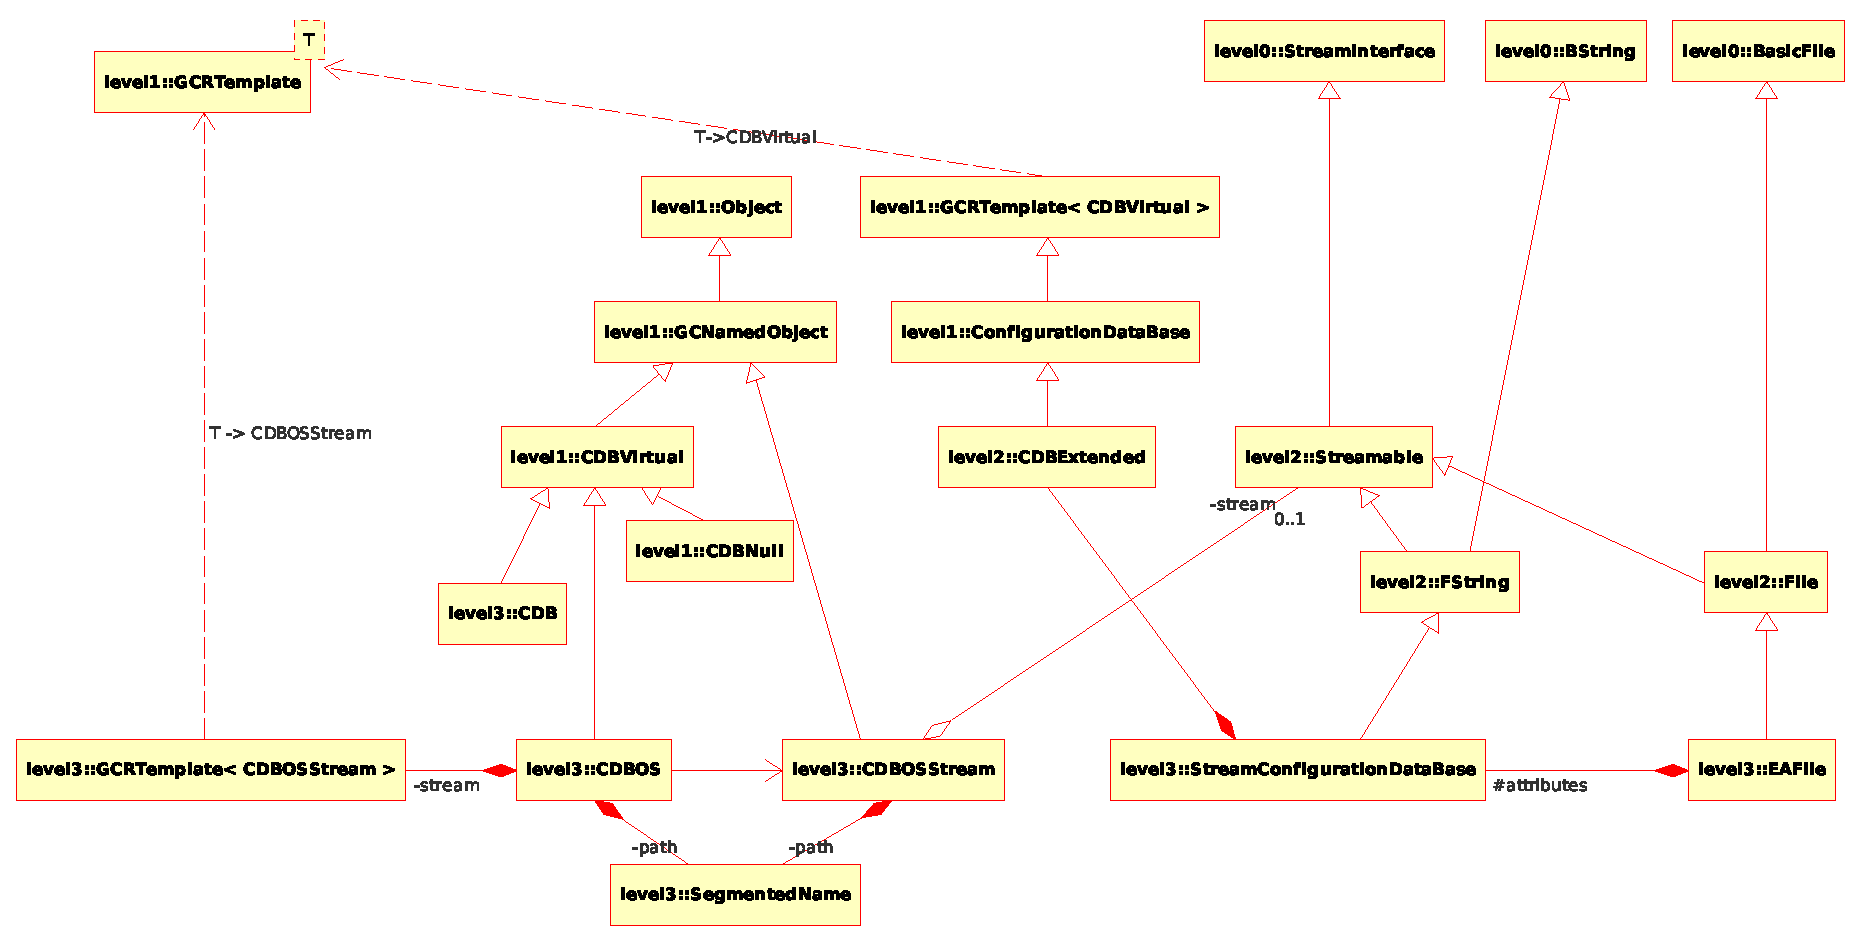
\includegraphics[width=\textwidth]{level3/level3-otherCDB.eps}
  \caption{BaseLib Level3 CDBOS and SCDB}
  \label{f:level3:otherCDB}
 \end{center}
\end{figure}



\subsection{CDBOS}
TODO\\
TODO\\
TODO\\
CHE COSA E e cosa fa

\begin{figure}[h!]
 \begin{center}
  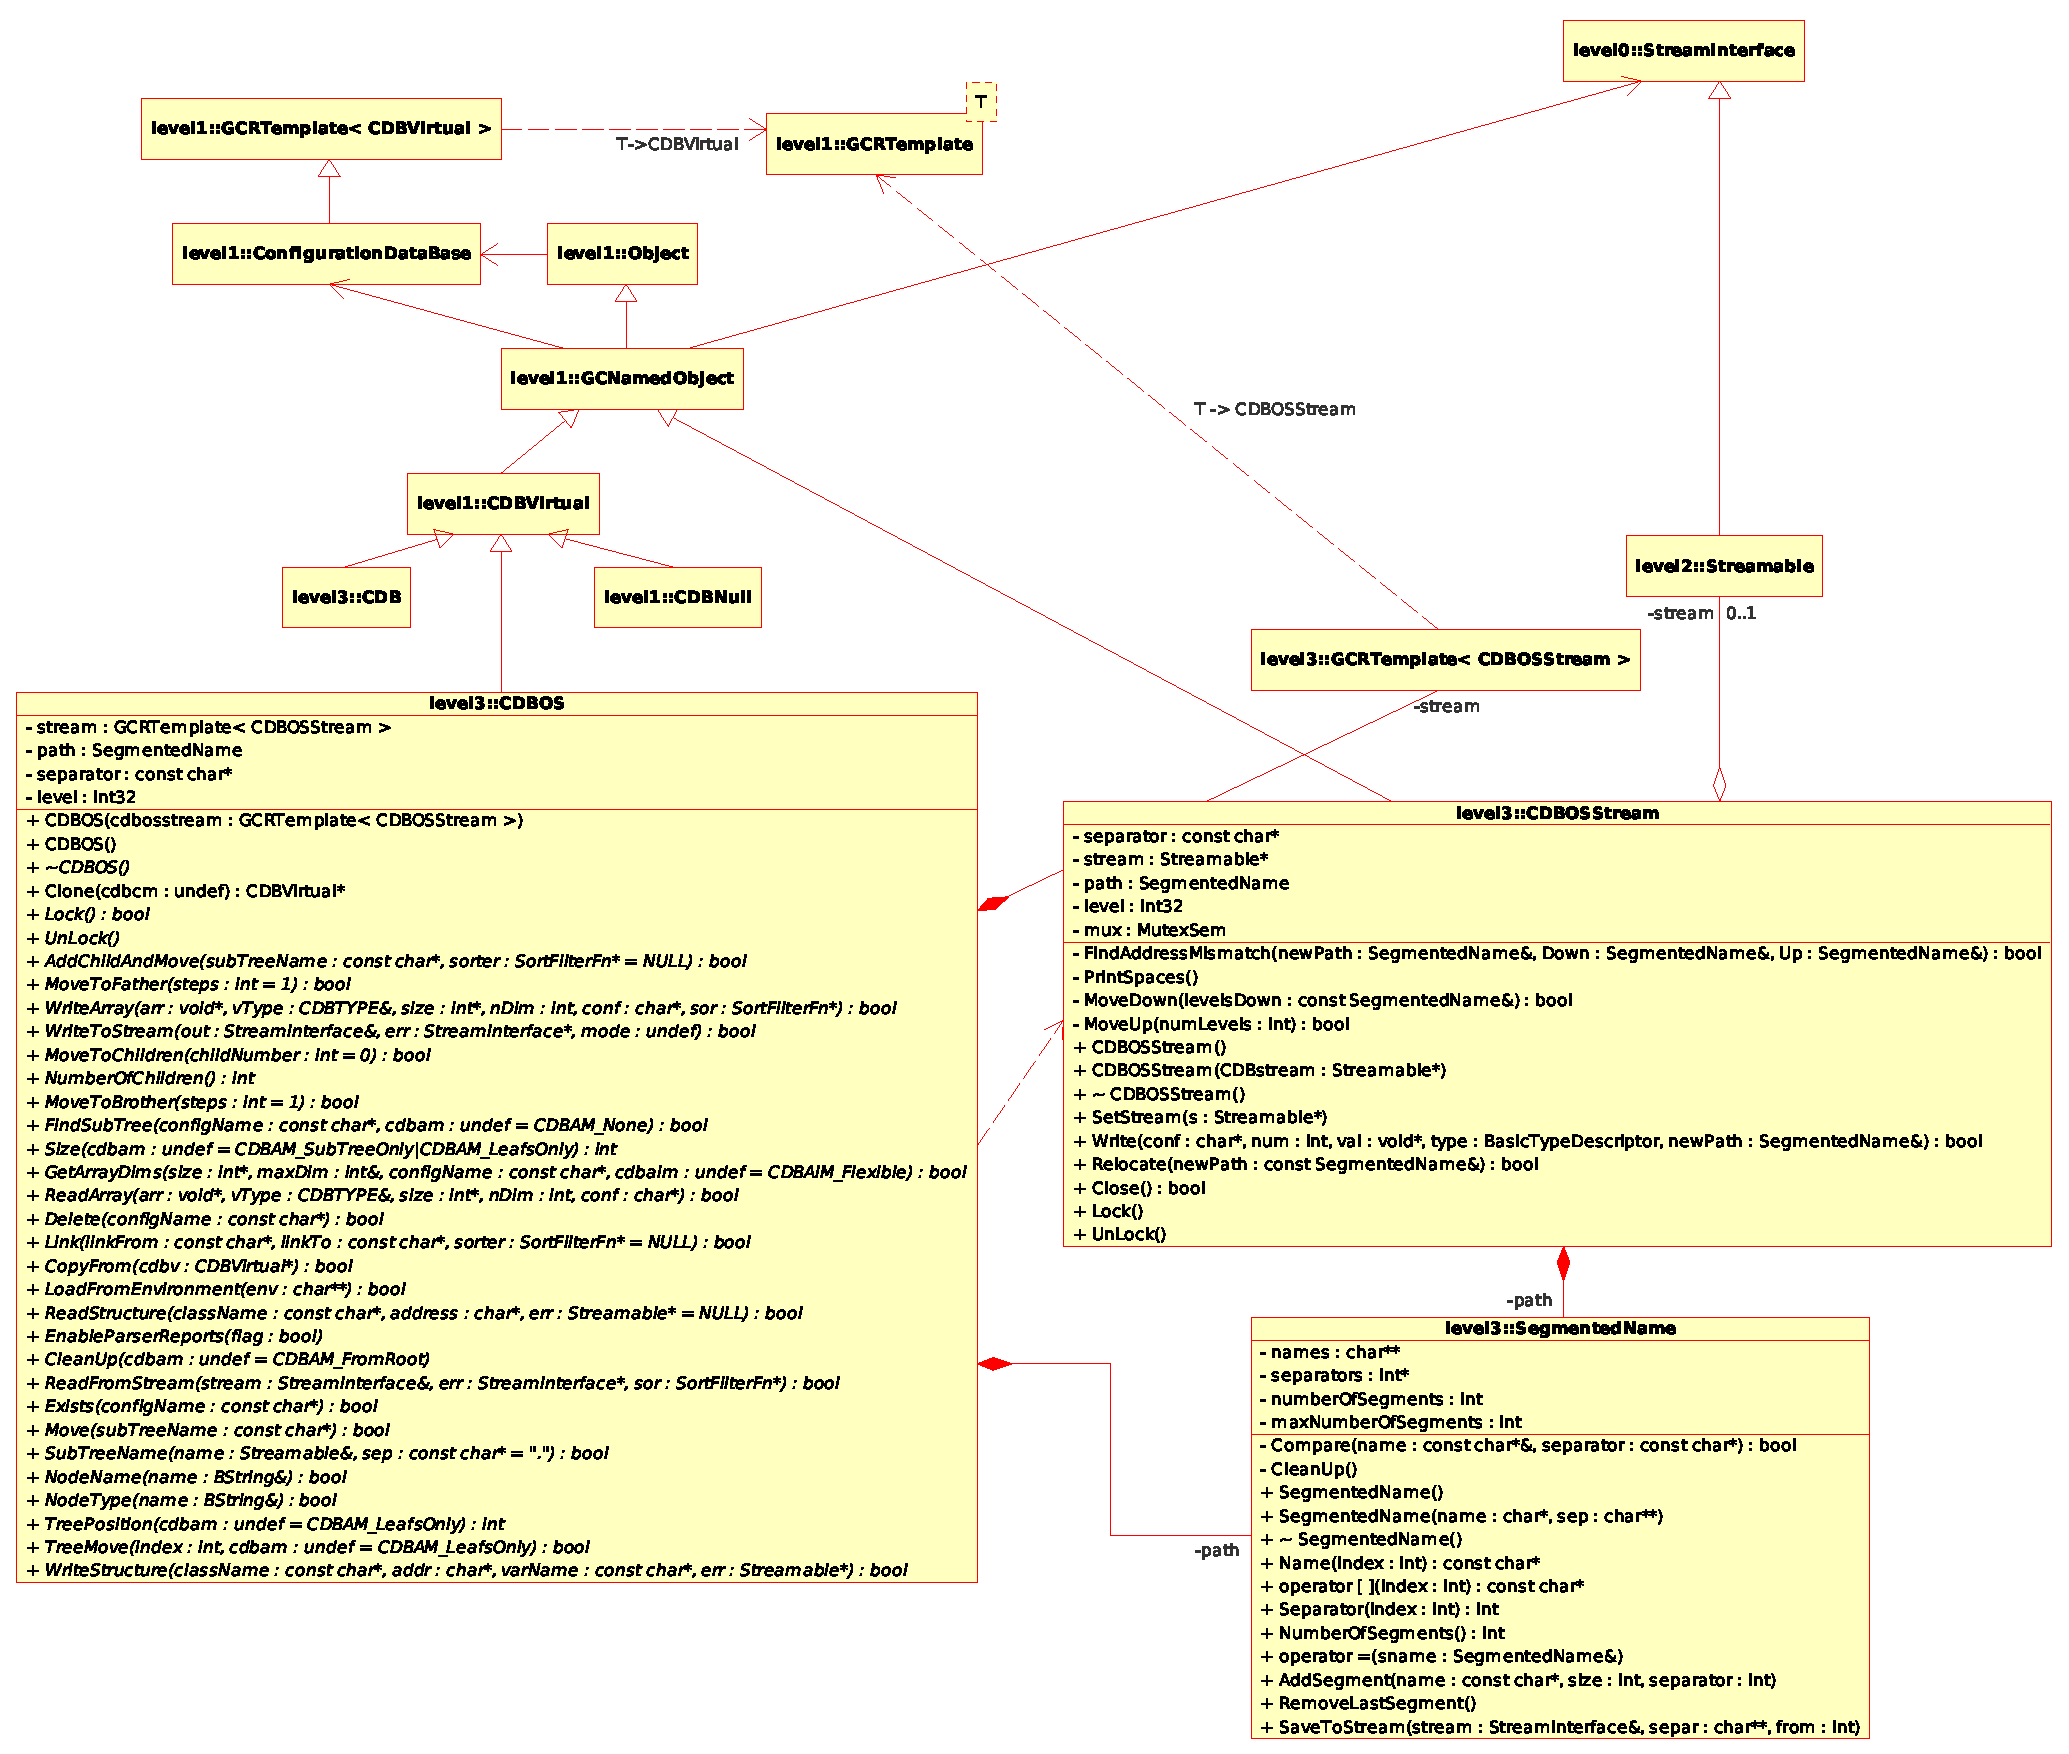
\includegraphics[width=\textwidth]{level3/level3-CDBOS.eps}
  \caption{BaseLib Level3 CDBOS (another Configuration Database implementation)}
  \label{f:level3:CDBOS}
 \end{center}
\end{figure}


\begin{itemize}
 \item SegmentedName
 \item CDBOSStream
 \item CDBOS
\end{itemize}



\subsubsection{SegmentedName}
\texttt{[SegmentedName.h]}\\
The class \texttt{SegmentedName} doesn't inherit from any other class. Such class parses a name with segments like paths or structure naming. For example it can be used to segment a UNIX path like this:

\begin{lstlisting}[
extendedchars=true,%
basicstyle=\fontfamily{pcr}\fontseries{m}\selectfont\footnotesize, %
stepnumber=1,%
numberstyle=\tiny,%
keywordstyle=\footnotesize\tt ,%
language=bash]
/usr/include/asm-generic/bitops/atomic.h
\end{lstlisting}

in two data structures: an array of character strings, the segments (attribute \texttt{names} see below the source), and an array of index of separators (attribute \texttt{separators}). The parsing of the path above load the class with the following contents:
\begin{table}[!h]
 \begin{center}
  \begin{tabular}{|c|c|c|}
   \hline
index & \texttt{char** names} & \texttt{int* separators} \\
    \hline
0 & usr & \texttt{/} \\
1 & include & \texttt{/} \\
2 & asm-generic & \texttt{/} \\
3 & bitops & \texttt{/} \\
4 & atomic & \texttt{/} \\
5 & h & \texttt{.} \\
    \hline
    \end{tabular}
   \end{center}
  \caption{Level3 \texttt{SegmentedName} class attributes}
 \label{t:level3:SegmentedName}
\end{table}

From the source we know the four attribtues on which the class is build up, the first attribute, \texttt{names} is a zero separated names array, \texttt{separators} is an index in the separators list provided at object construction (note that in the attribute list there is no such list). \texttt{numberOfSegments} is the current number of segments added to the list, \texttt{maxNumberOfSegments} is the actually max number of segments in the class.
\begin{lstlisting}[
extendedchars=true,%
basicstyle=\fontfamily{pcr}\fontseries{m}\selectfont\footnotesize, %
stepnumber=1,%
numberstyle=\tiny,%
keywordstyle=\footnotesize\tt ,%
language=C++]
private:
   char** names;
   int* separators;
   int numberOfSegments;
   int maxNumberOfSegments;
\end{lstlisting}

The method \texttt{Compare} is similar to the well known \texttt{strcmp} but limit search to size of separators, \texttt{CleanUp} simply free all associated structures (char strings) of a class.

Teh first constructor create a new \texttt{null} \texttt{SegmenetedName}, the second one take as arguments a character string containing a name to be segmented and a separators list, i.e. a \texttt{NULL} terminated vector of separators strings. \\


The method \texttt{Name} returns the \texttt{index}-th segment, \texttt{Separator} returns the index of the \texttt{index}-th separator in the string. \texttt{NumberOfSegments} returns the currently available segments in the class. Then two operator ridefinition are coming. \texttt{AddSegment} simply let you to add a segment manually, that you can remove with \texttt{RemoveLastSegment}. With the method \texttt{SaveToStream} it is possible to recompone the segmented name saved starting from any segment (see \texttt{fromSegment} argument).
\begin{lstlisting}[
extendedchars=true,%
basicstyle=\fontfamily{pcr}\fontseries{m}\selectfont\footnotesize, %
stepnumber=1,%
numberstyle=\tiny,%
keywordstyle=\footnotesize\tt ,%
language=C++]
   bool Compare(const char*& name,const char* separator);
   void CleanUp();

public:
   SegmentedName();
   SegmentedName(const char* name,const char** separatorNames);
   ~SegmentedName();

   const char* Name(int index) const;
   int Separator(int index);
   int NumberOfSegments() const;
   const char* operator[](int index) const;
   void operator=(SegmentedName& sname);

   void AddSegment(const char* name,int size,int separator);
   void RemoveLastSegment();
   void SaveToStream(StreamInterface& stream,const char** separatorNames=NULL,
      int fromSegment=0);
\end{lstlisting}



\subsubsection{CDBOSStream}
\texttt{[CDBOSStream.h]}\\
The class \texttt{CDBOSStream} is used from the class \texttt{CDBOS}, so it is presented before. \\


The first attribute is a character string \texttt{separator} that holds a list of separator, single character separators. The second attribute is a pointer to a \texttt{Streamable}, i.e. an interal pointer to the \texttt{Streamable} to write the \texttt{CDB} content. The attribute \texttt{path} is a \texttt{SegmentedName} that holds the current path in the CDB, \texttt{level} stores the current level in the hierarchy and the \texttt{MutexSem} protects against concurrent operations on the data structure.

\begin{lstlisting}[
extendedchars=true,%
basicstyle=\fontfamily{pcr}\fontseries{m}\selectfont\footnotesize, %
stepnumber=1,%
numberstyle=\tiny,%
keywordstyle=\footnotesize\tt ,%
language=C++]
private:
   const char* separator;
   Streamable* stream;
   SegmentedName path;
   int32 level;
   MutexSem mux;
\end{lstlisting}

We take a look at the methods of the class; method \texttt{FindAddressMismatch} finds differences between two \texttt{CDB} addresses; \texttt{PrintSpaces} prints spaces to respect hierarchy, \texttt{MoveDown} moves \textbf{n} levels down the structure and \texttt{MoveUp} moves \textbf{n} levels up the structure. \\


The constructor initialize the class by default with separator \texttt{``/''}. The method \texttt{SetStream} sets the \texttt{stream} attribute; \texttt{Write} writs to the output one value at the current address.
\texttt{Relocate} lets move in the CDB and update internal path; \texttt{Close} closes the parenthesis opened untill now; methods \texttt{Lock} and \texttt{UnLock} locks and unlock the stream's semaphore.
\begin{lstlisting}[
extendedchars=true,%
basicstyle=\fontfamily{pcr}\fontseries{m}\selectfont\footnotesize, %
stepnumber=1,%
numberstyle=\tiny,%
keywordstyle=\footnotesize\tt ,%
language=C++]
   bool FindAddressMismatch(const SegmentedName& newPath,int& levelsUp,
      SegmentedName& levelsDown);
   void PrintSpaces();
   bool MoveDown(const SegmentedName& levelsDown);
   bool MoveUp int numLevels);

public:
   CDBOSStream(): separator("/"), path("",&separator);
   CDBOSStream(Streamable* CDBstream) : separator("/"),path("",&separator);
   ~CDBOSStream();

   void SetStream(Streamable* s);
   bool Write (const char* configName,int numOfElements,const void* value,
      BasicTypeDescriptor type,const SegmentedName& newPath);

   bool Relocate (const SegmentedName& newPath);
   bool Close();
   void Lock();
   void UnLock();
\end{lstlisting}

The class \texttt{CDBOSStream} is used to templatize a \texttt{GCRTemplate} that is then used as an attribute in the following \texttt{CDBOS} class.



\subsubsection{CDBOS}
\texttt{[CDBOS.h, CDBOS.cpp]}\\
The class \texttt{CDBOS} inherits from \texttt{CDBVirtual}, the \texttt{CDBOS} implement direct writing of a \textit{Configuration Database} to a stream. The first attribute is a \texttt{GCRTemplate< CDBOSStream >}, i.e. an object that has a pointer to a \texttt{CDBOSStream}. The attribute \texttt{path} save the current path inside the \texttt{CDB}, \texttt{separator} is a character array of separators and \texttt{level} stores the current level in the hierarchy in the same way as they do in the \texttt{CDBOSStream} class.
\begin{lstlisting}[
extendedchars=true,%
basicstyle=\fontfamily{pcr}\fontseries{m}\selectfont\footnotesize, %
stepnumber=1,%
numberstyle=\tiny,%
keywordstyle=\footnotesize\tt ,%
language=C++]
private:
   GCRTemplate<CDBOSStream> stream;
   SegmentedName path;
   const char* separator;
   int32 level;

   CDBOS(GCRTemplate<CDBOSStream> cdbosstream) : separator("/"), path("",&separator);
   CDBOS() : stream(GCFT_Create), separator("/"), path("",&separator);
   virtual ~CDBOS();
\end{lstlisting}

The method \texttt{Clone} returns a \texttt{CDBVirtual} pointer creating a new reference to a database, or if that is not possible it creates a copy of it; if \texttt{cdbcm} is \texttt{CDBCM\_CopyAddress} ensures that the new object points at the same location.

The method \texttt{Lock} locks the main database for exclusive access: use if a group of transactions should be atomic; \texttt{UnLock} unlocks the main database: remember to unlock a locked database after using it.

The method \texttt{AddChilAndMove} can be used to create a new subtree, \texttt{MoveToFather} move the current pointer to the father's node, $-1$ means moving to the root node. \\


The method \texttt{WriteArray} calls the method \texttt{GCRTemplate< CDBOSStream >::Write}, if \texttt{size} is \texttt{NULL} it treats the input as a monodimensional array of size \texttt{nDim}. The method \texttt{WriteToStream} is used to write to the stream assigned.
\begin{lstlisting}[
extendedchars=true,%
basicstyle=\fontfamily{pcr}\fontseries{m}\selectfont\footnotesize, %
stepnumber=1,%
numberstyle=\tiny,%
keywordstyle=\footnotesize\tt ,%
language=C++]
public:
   CDBVirtual* Clone(CDBCreationMode cdbcm);
   virtual bool Lock();
   virtual void UnLock();

   virtual bool AddChildAndMove(const char* subTreeName,SortFilterFn* sorter=NULL);
   virtual bool MoveToFather(int steps=1);

   virtual bool WriteArray(const void* array,const CDBTYPE& valueType,const int* size,
      int nDim,const char* configName,SortFilterFn* sorter=NULL);
   virtual bool WriteToStream(StreamInterface& streamout,StreamInterface* err=NULL,
      CDBWriteMode mode=CDBWM_Tree);
\end{lstlisting}

Then follow a huge list of overridden methods that simply returns an error because are not implemented in this class.

\begin{lstlisting}[
extendedchars=true,%
basicstyle=\fontfamily{pcr}\fontseries{m}\selectfont\footnotesize, %
stepnumber=1,%
numberstyle=\tiny,%
keywordstyle=\footnotesize\tt ,%
language=C++]
    virtual bool MoveToChildren(int childNumber=0);
    virtual int  NumberOfChildren();
    virtual bool MoveToBrother(int steps=1);
    virtual bool FindSubTree(const char* configName,CDBAddressMode cdbam=CDBAM_None);
    virtual int  Size(CDBAddressMode cdbam=CDBAM_SubTreeOnly | CDBAM_LeafsOnly)
    virtual bool GetArrayDims(int* size,int& maxDim,const char* configName,CDBArrayIndexingMode cdbaim=CDBAIM_Flexible);
    virtual bool ReadArray(void* array,const CDBTYPE& valueType,const int* size,int nDim,const char* configName);
    virtual bool Delete(const char* configName);
    virtual bool Link(const char* linkFrom,const char* linkTo,SortFilterFn* sorter=NULL);
    virtual bool CopyFrom(CDBVirtual* cdbv);
    virtual bool LoadFromEnvironment(char** env);
    virtual bool ReadStructure (const char* className,char* address,Streamable* err=NULL);
    virtual void EnableParserReports(bool flag);
    virtual void CleanUp(CDBAddressMode cdbam=CDBAM_FromRoot);
    virtual bool ReadFromStream(StreamInterface& stream,StreamInterface* err=NULL,SortFilterFn* sorter=NULL);
    virtual bool Exists(const char* configName);
    virtual bool Move(const char* subTreeName);
    virtual bool SubTreeName(Streamable& name,const char* sep = ".")
    virtual bool NodeName(BString& name);
    virtual bool NodeType(BString& name);
    virtual int  TreePosition(CDBAddressMode cdbam=CDBAM_LeafsOnly);
    virtual bool TreeMove(int index,CDBAddressMode cdbam=CDBAM_LeafsOnly);
    virtual bool WriteStructure(const char* className,char* address,const char* variableName=NULL,Streamable* err=NULL);
\end{lstlisting}



\subsection{Stream Configuration Database (SCDB)}
The \textit{Stream Configuration Database} is another kind of \textit{Configuration Database} that is really similar to the \texttt{CDBOS} structure.
Figure \ref{f:level3:SCDB} represent the UML schema of the \textit{Stream Configuration Database} infrastructure.
Classes in this section are:
\begin{itemize}
 \item StreamConfigurationDataBase
 \item EAFile
\end{itemize}
The \texttt{EAFile} is grouped in this section because it is the only user of the SCDB in this section.
\begin{figure}[h!]
 \begin{center}
  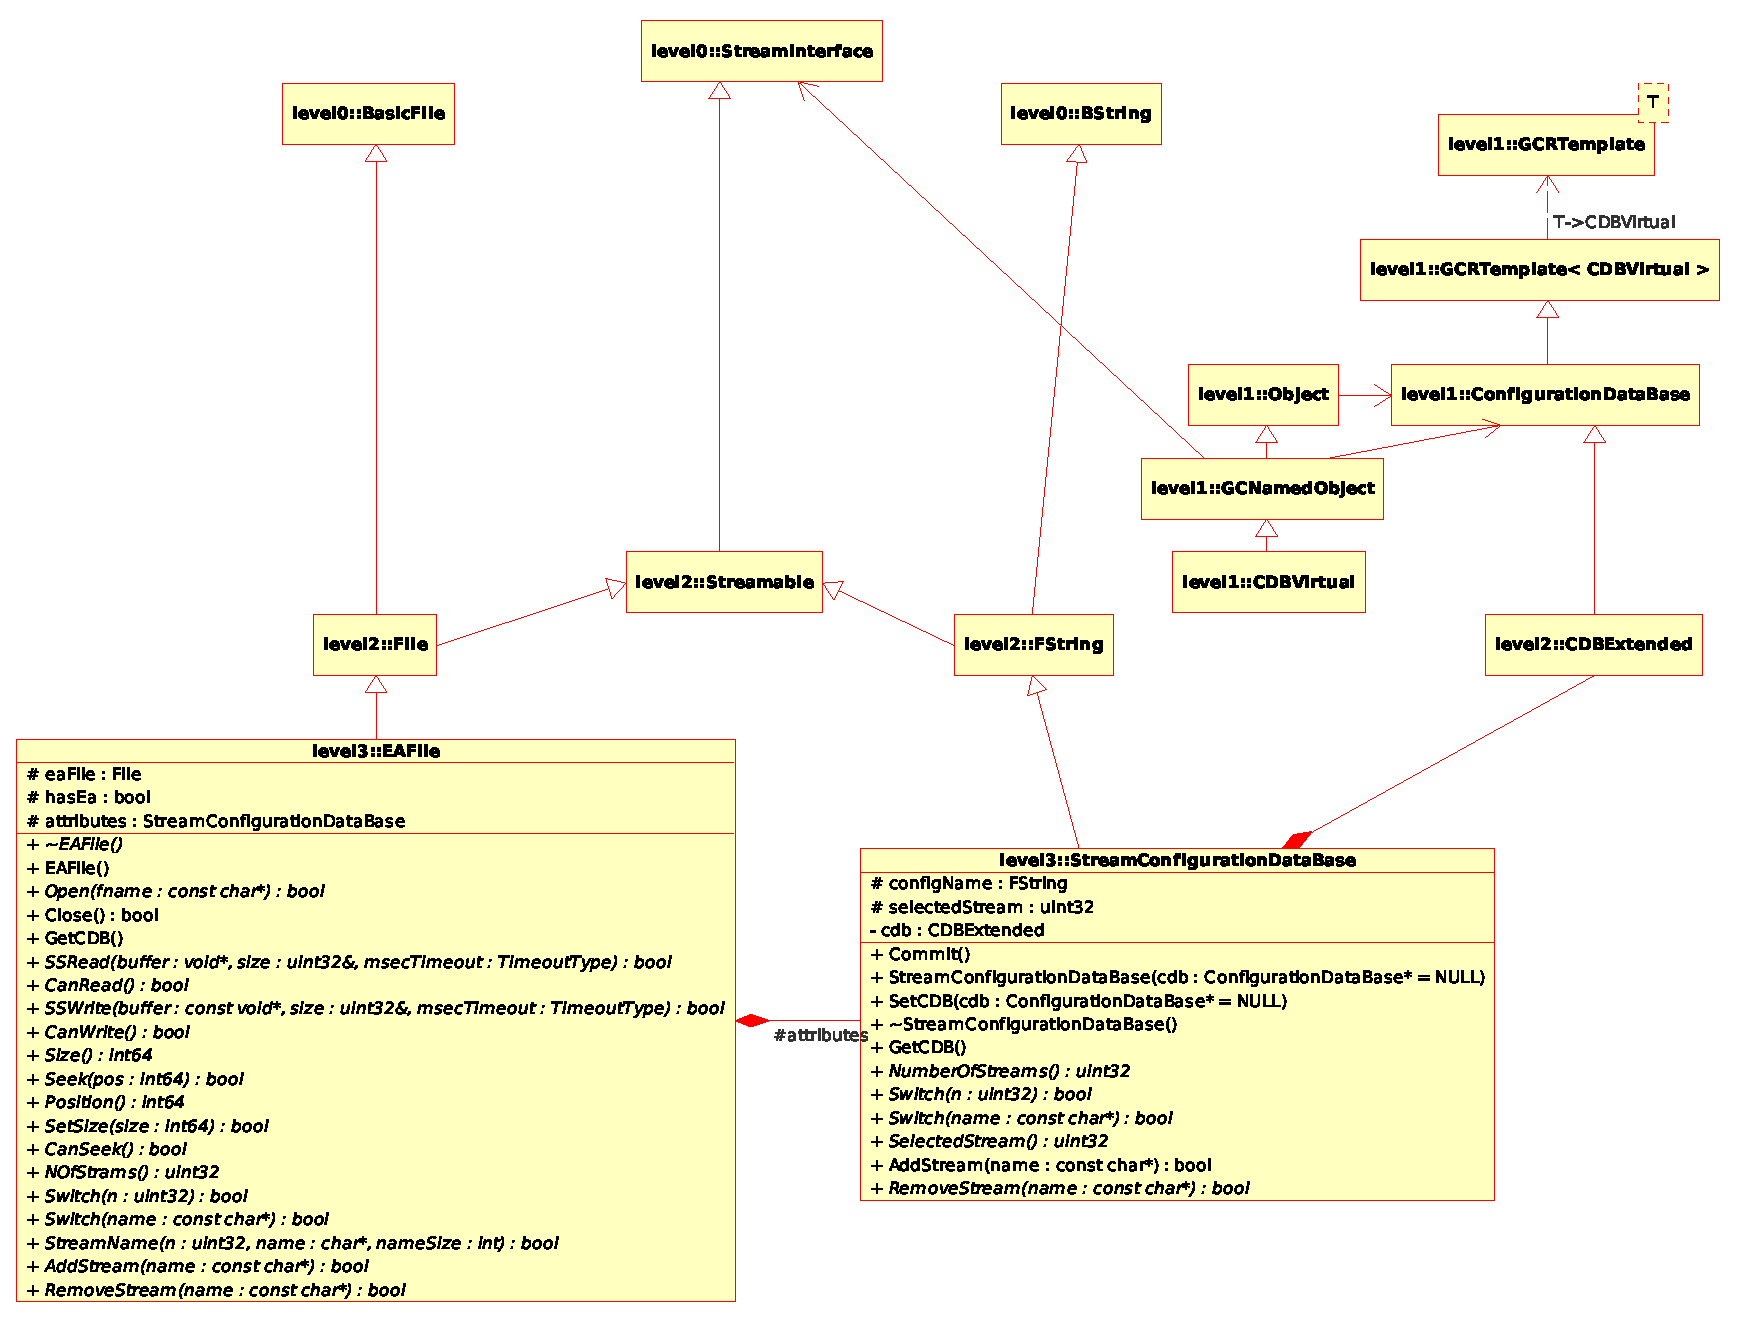
\includegraphics[width=\textwidth]{level3/level3-SCDB.eps}
  \caption{BaseLib Level3 SCDB (another Configuration Database implementation)}
  \label{f:level3:SCDB}
 \end{center}
\end{figure}



\subsubsection{StreamConfigurationDataBase}
\texttt{[StreamConfigurationDataBase.h, StreamConfigurationDataBase.cpp]}\\
The class \texttt{StreamConfigurationDataBase} implement a \textit{Configuration Database} using the multi stream interface to read and write data into, so it is far different from the \texttt{CDBOS} because is a \texttt{Streamable}, more precisely a \texttt{FString}, that has a \texttt{CDBExtended} as an attribute. With a SCDB it is possible to write and read to a CDB like a stream. \\


The first attribute \texttt{cdb} is the \texttt{CDBExtended} associated to the SCDB, i.e. the CDB being modified; \texttt{configName} is the current location pointer and \texttt{selectedStream} is the order of current location within tree.
\begin{lstlisting}[
extendedchars=true,%
basicstyle=\fontfamily{pcr}\fontseries{m}\selectfont\footnotesize, %
stepnumber=1,%
numberstyle=\tiny,%
keywordstyle=\footnotesize\tt ,%
language=C++]
protected:
   CDBExtended cdb;
   FString configName;
   uint32 selectedStream;
\end{lstlisting}

The method \texttt{Commit} copies the work done to the stream this far to the database, the constructor initialises with a reference to a \textit{CDB} the destructor basically calls \texttt{Commit} and \texttt{SetCDB} like the constructor initialises with a reference \textit{CDB}; \texttt{GetCDB} gets the \texttt{cdb} attribute. \\


The method \texttt{NumberOfStreams} returns how many streams are available in total, counts from root all the leaves. \texttt{SelectedStream} returns which is the selected stream. Methods \texttt{Switch} select the stream to read from, switching may reset the stream to the start. The method \texttt{AddStream} adds a new stream to write to and \texttt{RemoveStream} removes an existing stream.
\begin{lstlisting}[
extendedchars=true,%
basicstyle=\fontfamily{pcr}\fontseries{m}\selectfont\footnotesize, %
stepnumber=1,%
numberstyle=\tiny,%
keywordstyle=\footnotesize\tt ,%
language=C++]
public:
   void Commit();

   StreamConfigurationDataBase(ConfigurationDataBase* cdb = NULL):cdb("CDB");
   ~StreamConfigurationDataBase();

   void SetCDB(ConfigurationDataBase* cdb = NULL);
   CDBExtended& GetCDB();

   virtual uint32 NumberOfStreams();
   virtual uint32 SelectedStream();
   virtual bool Switch(uint32 n);
   virtual bool Switch(const char *name);

   bool AddStream(const char *name);
   virtual bool RemoveStream(const char *name){
\end{lstlisting}



\subsubsection{EAFile}
\texttt{[EAFile.h, EAFile.cpp]}\\
The class \texttt{EAFile} stands for \textit{Extended Attributes File}, it accounts to store extended attributes of files that a File Systema of an OS doesn't account for in a separate file; such files have the following extension, we paste the definition below.
\begin{lstlisting}[
extendedchars=true,%
basicstyle=\fontfamily{pcr}\fontseries{m}\selectfont\footnotesize, %
stepnumber=1,%
numberstyle=\tiny,%
keywordstyle=\footnotesize\tt ,%
language=C++]
#define EA_EXT ".!EA!"
\end{lstlisting}

The class inherits from \texttt{File} so its a \texttt{Streamable}. The first atrribute, \texttt{eaFile} is a \texttt{File} so it not only inherits from \texttt{File} but has also an attribute of the same type, and such attribute refers to the file containing the attributes. \texttt{hasEa} is \texttt{true} if any attributes have been set; \texttt{attributes} is a stream interface to the attributes.
\begin{lstlisting}[
extendedchars=true,%
basicstyle=\fontfamily{pcr}\fontseries{m}\selectfont\footnotesize, %
stepnumber=1,%
numberstyle=\tiny,%
keywordstyle=\footnotesize\tt ,%
language=C++]
protected:
   File eaFile;
   bool hasEa;
   StreamConfigurationDataBase attributes;
\end{lstlisting}

We skip destructor and constructor because are without arguments. The \texttt{Open} method opens for read/write or create if missing the \textit{Extended Attribute File}, \texttt{Close} closes it. \texttt{GetCDB} get the \texttt{attribute} attribute content. All other methos are from the \texttt{Streamable} interface. \\


The method \texttt{SSRead} reads from the selected stream, \texttt{SSWrite} writes to the selected stream, methods \texttt{CanRead} and \texttt{CanWrite} return the capability of reading and writing of the \texttt{attribute}.
\begin{lstlisting}[
extendedchars=true,%
basicstyle=\fontfamily{pcr}\fontseries{m}\selectfont\footnotesize, %
stepnumber=1,%
numberstyle=\tiny,%
keywordstyle=\footnotesize\tt ,%
language=C++]
public:
   virtual ~EAFile();
   EAFile()

   virtual bool Open(const char *fname,...);
   bool Close();

   CDBExtended& GetCDB();

   virtual bool SSRead (void* buffer,uint32& size,TimeoutType msecTimeout);
   virtual bool CanRead();
   virtual bool SSWrite(const void* buffer,uint32& size,TimeoutType msecTimeout);
   virtual bool CanWrite();
\end{lstlisting}

The method \texttt{Size} returns the size of the file; \texttt{SetSize} clips the file size to a specified point; \texttt{Position} returns the current position in the file; \texttt{Seek} moves within the file to an absolute location, \texttt{CanSeek} return \texttt{true} if seeking is possible. \\


The method \texttt{NOfStreams} gets how many streams are available; methods \texttt{Switch} select the stream to read from, switching may reset the stream to the start. \texttt{StreamName} returns the name of the stream \texttt{n}, stream \texttt{0} is the file and therefore you get the file name. \texttt{AddStream} adds a new stream to write to, \texttt{selectedStream} is resetted to \texttt{0}; \texttt{RemoveStream} removes a stream.
\begin{lstlisting}[
extendedchars=true,%
basicstyle=\fontfamily{pcr}\fontseries{m}\selectfont\footnotesize, %
stepnumber=1,%
numberstyle=\tiny,%
keywordstyle=\footnotesize\tt ,%
language=C++]
   virtual int64 Size();
   virtual bool SetSize(int64 size);
   virtual int64 Position(void);
   virtual bool Seek(int64 pos);
   virtual bool CanSeek();

   virtual uint32 NOfStreams();
   virtual bool Switch(uint32 n);
   virtual bool Switch(const char* name);
   virtual bool StreamName(uint32 n,char* name,int nameSize);
   virtual bool AddStream(const char* name);
   virtual bool RemoveStream(const char* name)
\end{lstlisting}



\subsection{Design Notes}
The class \texttt{SegmentedName} supports separators of only one character. How it is possible to handle separators made up of one or more characters, i.e. how it is possible to handle an URL like
\begin{lstlisting}[
extendedchars=true,%
basicstyle=\fontfamily{pcr}\fontseries{m}\selectfont\footnotesize, %
stepnumber=1,%
numberstyle=\tiny,%
keywordstyle=\footnotesize\tt ,%
language=bash]
http://www.google.it
\end{lstlisting}


\section{Parser}
The following classes address the problem of parsing a string, all classes create a framework to build up a parser.
In Figure \ref{f:level3:parser} is depicted the UML schema of the parser infrastructure.
The following classes are involved:
\begin{itemize}
 \item LA\_TokenInfo
 \item LA\_TokenData
 \item LexicalAnalyzer
 \item Parser
\end{itemize}

\begin{figure}[h!]
 \begin{center}
  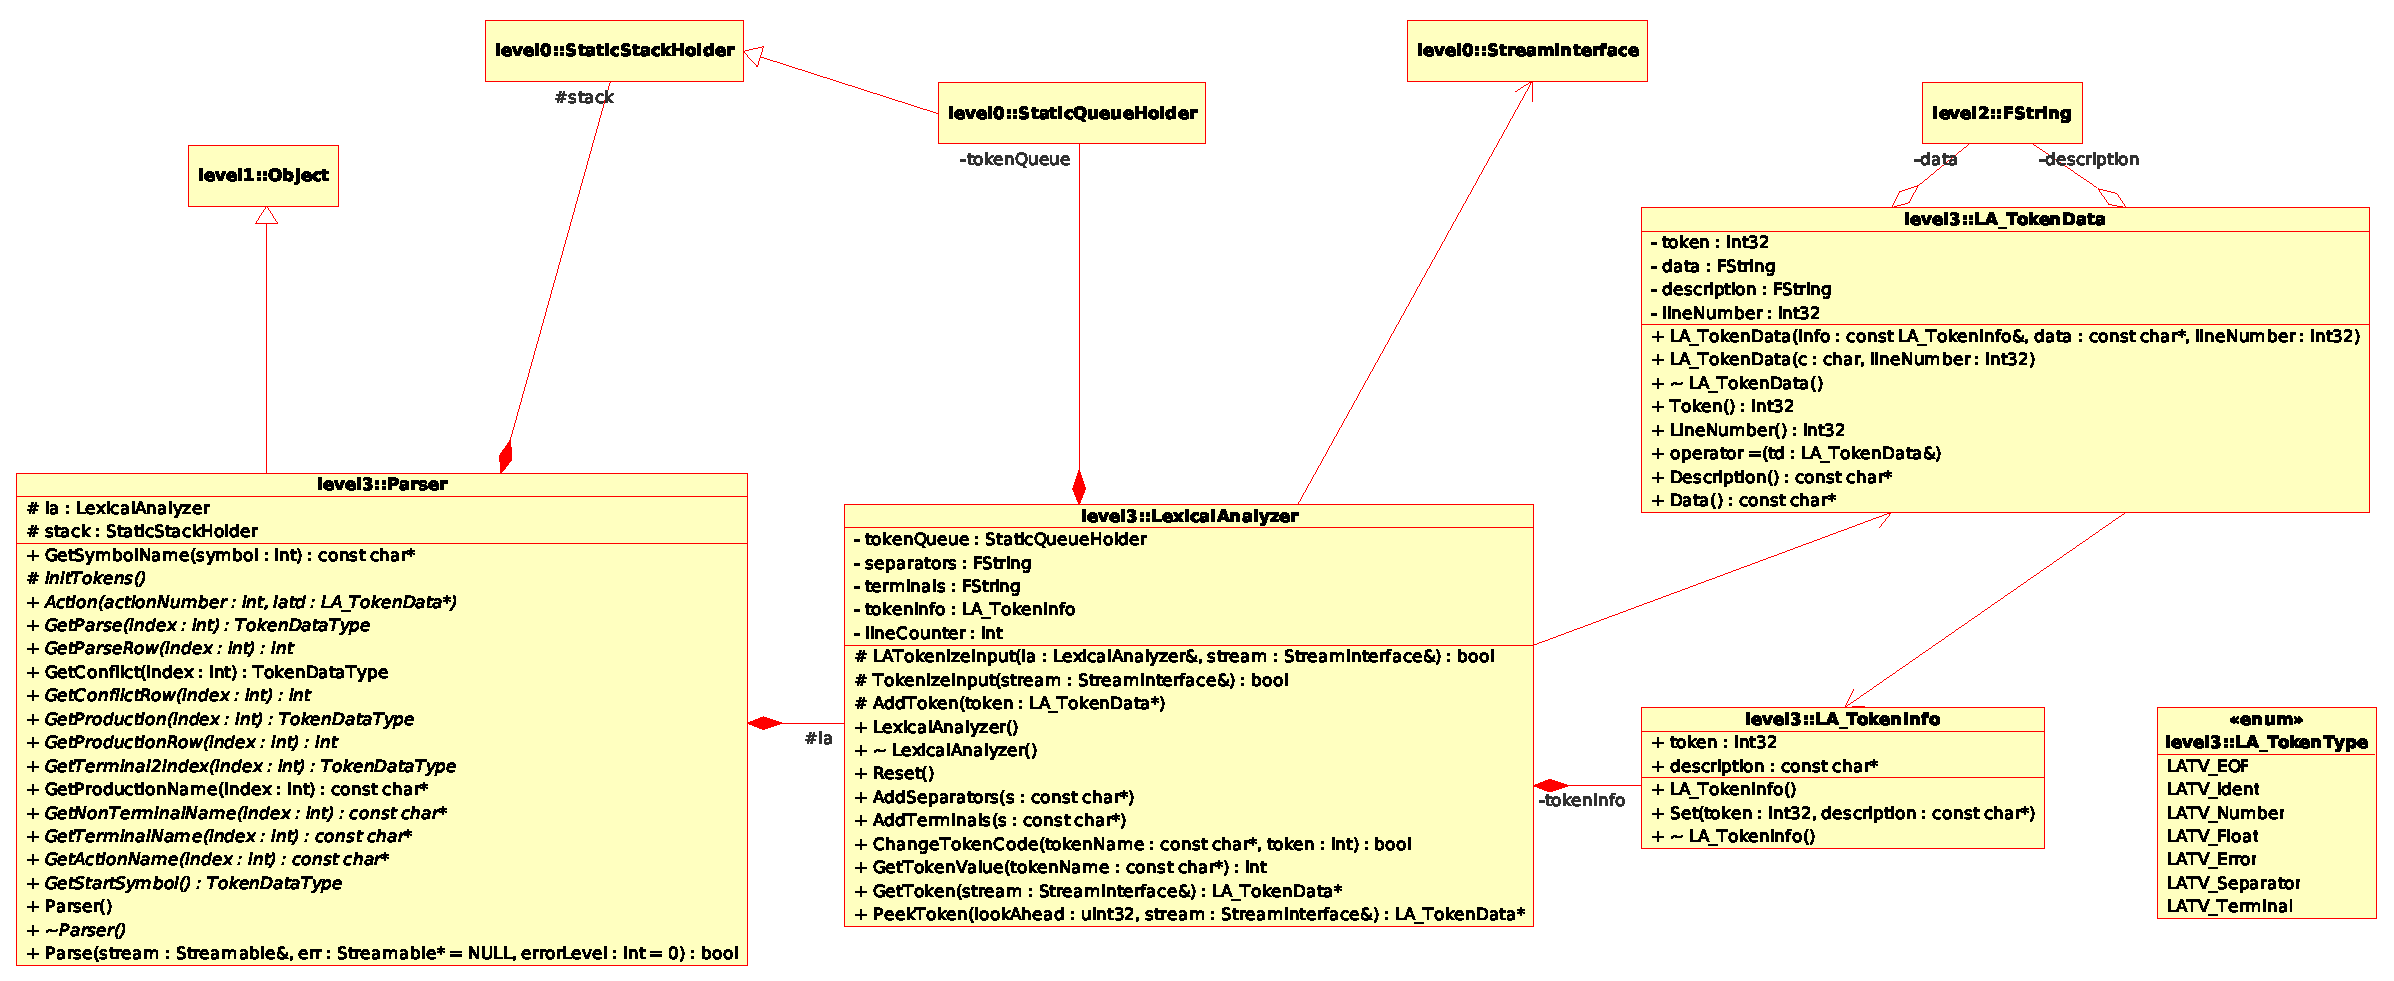
\includegraphics[width=\textwidth]{level3/level3-parser.eps}
  \caption{BaseLib Level3 parser, lexical analyser and tokenizer}
  \label{f:level3:parser}
 \end{center}
\end{figure}



\subsubsection{Lexical Analyzer Token Information}
\texttt{[LexicalAnalyzer.h, LexicalAnalyzer.cpp]}\\
The class \texttt{LA\_TokenInfo} stores information about a lexical element. The first attribute, \texttt{token} is the code identifying the lexical meaning of this part of the text, \texttt{description} holds the meaning of the token.
The constructor initialize \texttt{token} to zero and \texttt{description} to \texttt{NULL}, the method \texttt{Set} lets you setting the attributes.
\begin{lstlisting}[
extendedchars=true,%
basicstyle=\fontfamily{pcr}\fontseries{m}\selectfont\footnotesize, %
stepnumber=1,%
numberstyle=\tiny,%
keywordstyle=\footnotesize\tt ,%
language=C++]
public:
   int32 token;
   const char* description;

   LA_TokenInfo();
   ~LA_TokenInfo();
   void Set(int32 token,const char* description);
\end{lstlisting}



\subsubsection{Lexical Analyzer Token Data}
\texttt{[LexicalAnalyzer.h, LexicalAnalyzer.cpp]}\\
The class \texttt{LA\_TokenData} is an element produced by the \texttt{LexicalAnalyzer}. The attribute \texttt{token} is the code identifying the lexical meaning of this part of the text; \texttt{data} is the parsed part of the text; \texttt{description} is copied from a \texttt{LA\_TokenInfo}, it holds the meaning of the token; \texttt{lineNumber} saves at what line the token was found.
\begin{lstlisting}[
extendedchars=true,%
basicstyle=\fontfamily{pcr}\fontseries{m}\selectfont\footnotesize, %
stepnumber=1,%
numberstyle=\tiny,%
keywordstyle=\footnotesize\tt ,%
language=C++]
   int32 token;
   FString data;
   FString description;
   int32 lineNumber;
\end{lstlisting}

The first constructor builds a token from a token description constant and the data content, the second constructor builds a token from a simple character.

The method \texttt{Token} returns the attribute \texttt{token}; \texttt{LineNumber} returns the attribute \texttt{lineNumber}; the \texttt{operator=} redefinition copies content, \texttt{Description} return the description of the content and \texttt{Data} return the content, i.e. \texttt{data} attribute.
\begin{lstlisting}[
extendedchars=true,%
basicstyle=\fontfamily{pcr}\fontseries{m}\selectfont\footnotesize, %
stepnumber=1,%
numberstyle=\tiny,%
keywordstyle=\footnotesize\tt ,%
language=C++]
public:
   LA_TokenData(const LA_TokenInfo &info, const char *data,int32 lineNumber);
   LA_TokenData(char c,int32 lineNumber);
   virtual ~LA_TokenData();

   int32 Token();
   int32 LineNumber();
   void  operator=(LA_TokenData& td);
   const char* Description();
   const char* Data();
\end{lstlisting}



\subsubsection{Lexical Analyzer}
\texttt{[LexicalAnalyzer.h, LexicalAnalyzer.cpp]}\\
The class \texttt{LexicalAnalyzer} is a slightly programmable lexical analyzer; It recognizes \textit{identifiers}, \textit{numbers} and \textit{floats}. It allows to browse ahead without consuming the token, tokenisation is performed on demand.\\


Before exploring the class we paste an enumeration below. This enumeration is a set of codes to list the complex terminals recognised by the analyser. The source code is self explained.
\begin{lstlisting}[
extendedchars=true,%
basicstyle=\fontfamily{pcr}\fontseries{m}\selectfont\footnotesize, %
stepnumber=1,%
numberstyle=\tiny,%
keywordstyle=\footnotesize\tt ,%
language=C++]
enum LA_TokenType{
   /** indicates EOF */
   LATV_EOF=0x100,
   /** indicates an identifier or a string */
   LATV_Ident=0x101,
   /** indicates an integer */
   LATV_Number=0x102,
   /** indicates a float */
   LATV_Float=0x103,
   /** indicates a wrongly constructed element */
   LATV_Error=0x104,
   /** indicates an element that separates parts of the phrase */
   LATV_Separator=0x105,
   /** indicates an element that is a token on its own */
   LATV_Terminal=0x106
};
\end{lstlisting}

The first attribute, \texttt{tokenQueue} is a queue of pre-cooked tokens; \texttt{separators} is a string made of separators; \texttt{terminals} is a string composed of the terminal characters; \texttt{tokenInfo} list of token informations.
\begin{lstlisting}[
extendedchars=true,%
basicstyle=\fontfamily{pcr}\fontseries{m}\selectfont\footnotesize, %
stepnumber=1,%
numberstyle=\tiny,%
keywordstyle=\footnotesize\tt ,%
language=C++]
   StaticQueueHolder tokenQueue;
   FString separators;
   FString terminals;
   LA_TokenInfo tokenInfo[LATV_Error+2-0x100];
   int lineCounter;
\end{lstlisting}

The method \texttt{TokenizeInput} is the main method that takes as an argument a \texttt{StreamInterface} and with the \texttt{this} pointer calls a friend C method \texttt{LA\_TokenizeInput} that make the tokenization of the input stream; every token is also added to the \texttt{tokenQueue}.

The method \texttt{AddToken} adds a token into the \texttt{tokenQueue}. \texttt{Reset} resets the status of the class; \texttt{AddSeparators} sets these characters as separators; \texttt{AddTerminals} sets these characters as separators; \texttt{ChangeTokenCode} changes the token code associated with a given complex terminal, valid \texttt{tokenNames} are:
\begin{itemize}
 \item "EOF"
 \item "IDENT"
 \item "NUMBER"
 \item "FLOAT"
 \item "ERROR"
\end{itemize}

The method \texttt{GetToken} takes one token from the stack or processes the input for a new one, moves the token into last token. The class allocates the data but does not provide to the deallocation once the structure has been extracted.
The method \texttt{PeekToken} reads in the stack at position \texttt{lookAhead} argument or increases the stack to allow for it; it returns the token but it still keeps hold of it.

\begin{lstlisting}[
extendedchars=true,%
basicstyle=\fontfamily{pcr}\fontseries{m}\selectfont\footnotesize, %
stepnumber=1,%
numberstyle=\tiny,%
keywordstyle=\footnotesize\tt ,%
language=C++]
protected:
   bool TokenizeInput(StreamInterface &stream);
   void AddToken(LA_TokenData* token);

public:
   LexicalAnalyzer(): tokenQueue(sizeof(LA_TokenData*)/sizeof(int));
   ~LexicalAnalyzer()

   void Reset();
   void AddSeparators(const char* s);
   void AddTerminals(const char* s);
   bool ChangeTokenCode(const char* tokenName,int token);

   int GetTokenValue(const char* tokenName);

   LA_TokenData* GetToken(StreamInterface& stream);
   LA_TokenData* PeekToken(uint32 lookAhead,StreamInterface& stream);
\end{lstlisting}



\subsubsection{Parser}
\texttt{[Parser.h, Parser.cpp]}\\
The class \texttt{Parser} allows implementation of parsers. It is a base class for parsers. The class inherits from \texttt{Object}. The first attribute, of type \texttt{LexicalAnalyzer}, is the lexical analyzer; second attribute is a \texttt{StaticStackHolder}. \\


The method \texttt{GetSymbolName} gets the symbol name from an index. The method \texttt{Parse} 
parses a \texttt{Streamable} passed by argument, \texttt{errorLevel} can be one of the following:
\begin{itemize}
 \item \texttt{0} means do not display
 \item \texttt{1} means show actions
 \item \texttt{2} means show productions
 \item \texttt{-1} means show all
\end{itemize}

\begin{lstlisting}[
extendedchars=true,%
basicstyle=\fontfamily{pcr}\fontseries{m}\selectfont\footnotesize, %
stepnumber=1,%
numberstyle=\tiny,%
keywordstyle=\footnotesize\tt ,%
language=C++]
protected:
   LexicalAnalyzer la;
   StaticStackHolder stack;
private:
   const char* GetSymbolName(int symbol);
public:
   Parser():stack(sizeof(TokenDataType)/sizeof(int));
   virtual ~Parser();
   bool Parse(Streamable& stream,Streamable* err=NULL,int errorLevel=0);
\end{lstlisting}

Then follows a great set of pure virtual methods that must be implemented in \texttt{Parser}'s subclasses. Actually in BaseLib there is no class that make use or extends such class.

\begin{lstlisting}[
extendedchars=true,%
basicstyle=\fontfamily{pcr}\fontseries{m}\selectfont\footnotesize, %
stepnumber=1,%
numberstyle=\tiny,%
keywordstyle=\footnotesize\tt ,%
language=C++]
protected:
   virtual void InitTokens()=0;
   virtual void Action(int actionNumber,LA_TokenData* latd)=0;
   virtual TokenDataType GetParse(int index)=0;
   virtual int GetParseRow(int index)=0;
   virtual TokenDataType GetConflict(int index)=0;
   virtual int GetConflictRow(int index)=0;
   virtual TokenDataType GetProduction(int index)=0;
   virtual int GetProductionRow(int index)=0;
   virtual TokenDataType GetTerminal2Index(int index)=0;
   virtual const char* GetProductionName(int index)=0;
   virtual const char* GetNonTerminalName(int index)=0;
   virtual const char* GetTerminalName(int index)=0;
   virtual const char* GetActionName(int index)=0;
   virtual TokenDataType GetStartSymbol()=0;
\end{lstlisting}



\subsection{Design Notes}
Never used in BaseLib.


\chapter{BaseLib Level 4}
\chaptermark{Level 4}

BaseLib Level 4 integrate full HTTP protocol, server and client side. The server can manage more than one client at a time and the stream is usually coded in HTML version 1.0 with support to the \textit{keep alive} functionality. There is also an approach to manage secure connection letting the developer which pages are for public domain and which are only for selected users defining a sort of policy security.



\section{HttpStream and URLs}


\begin{figure}[h!]
 \begin{center}
  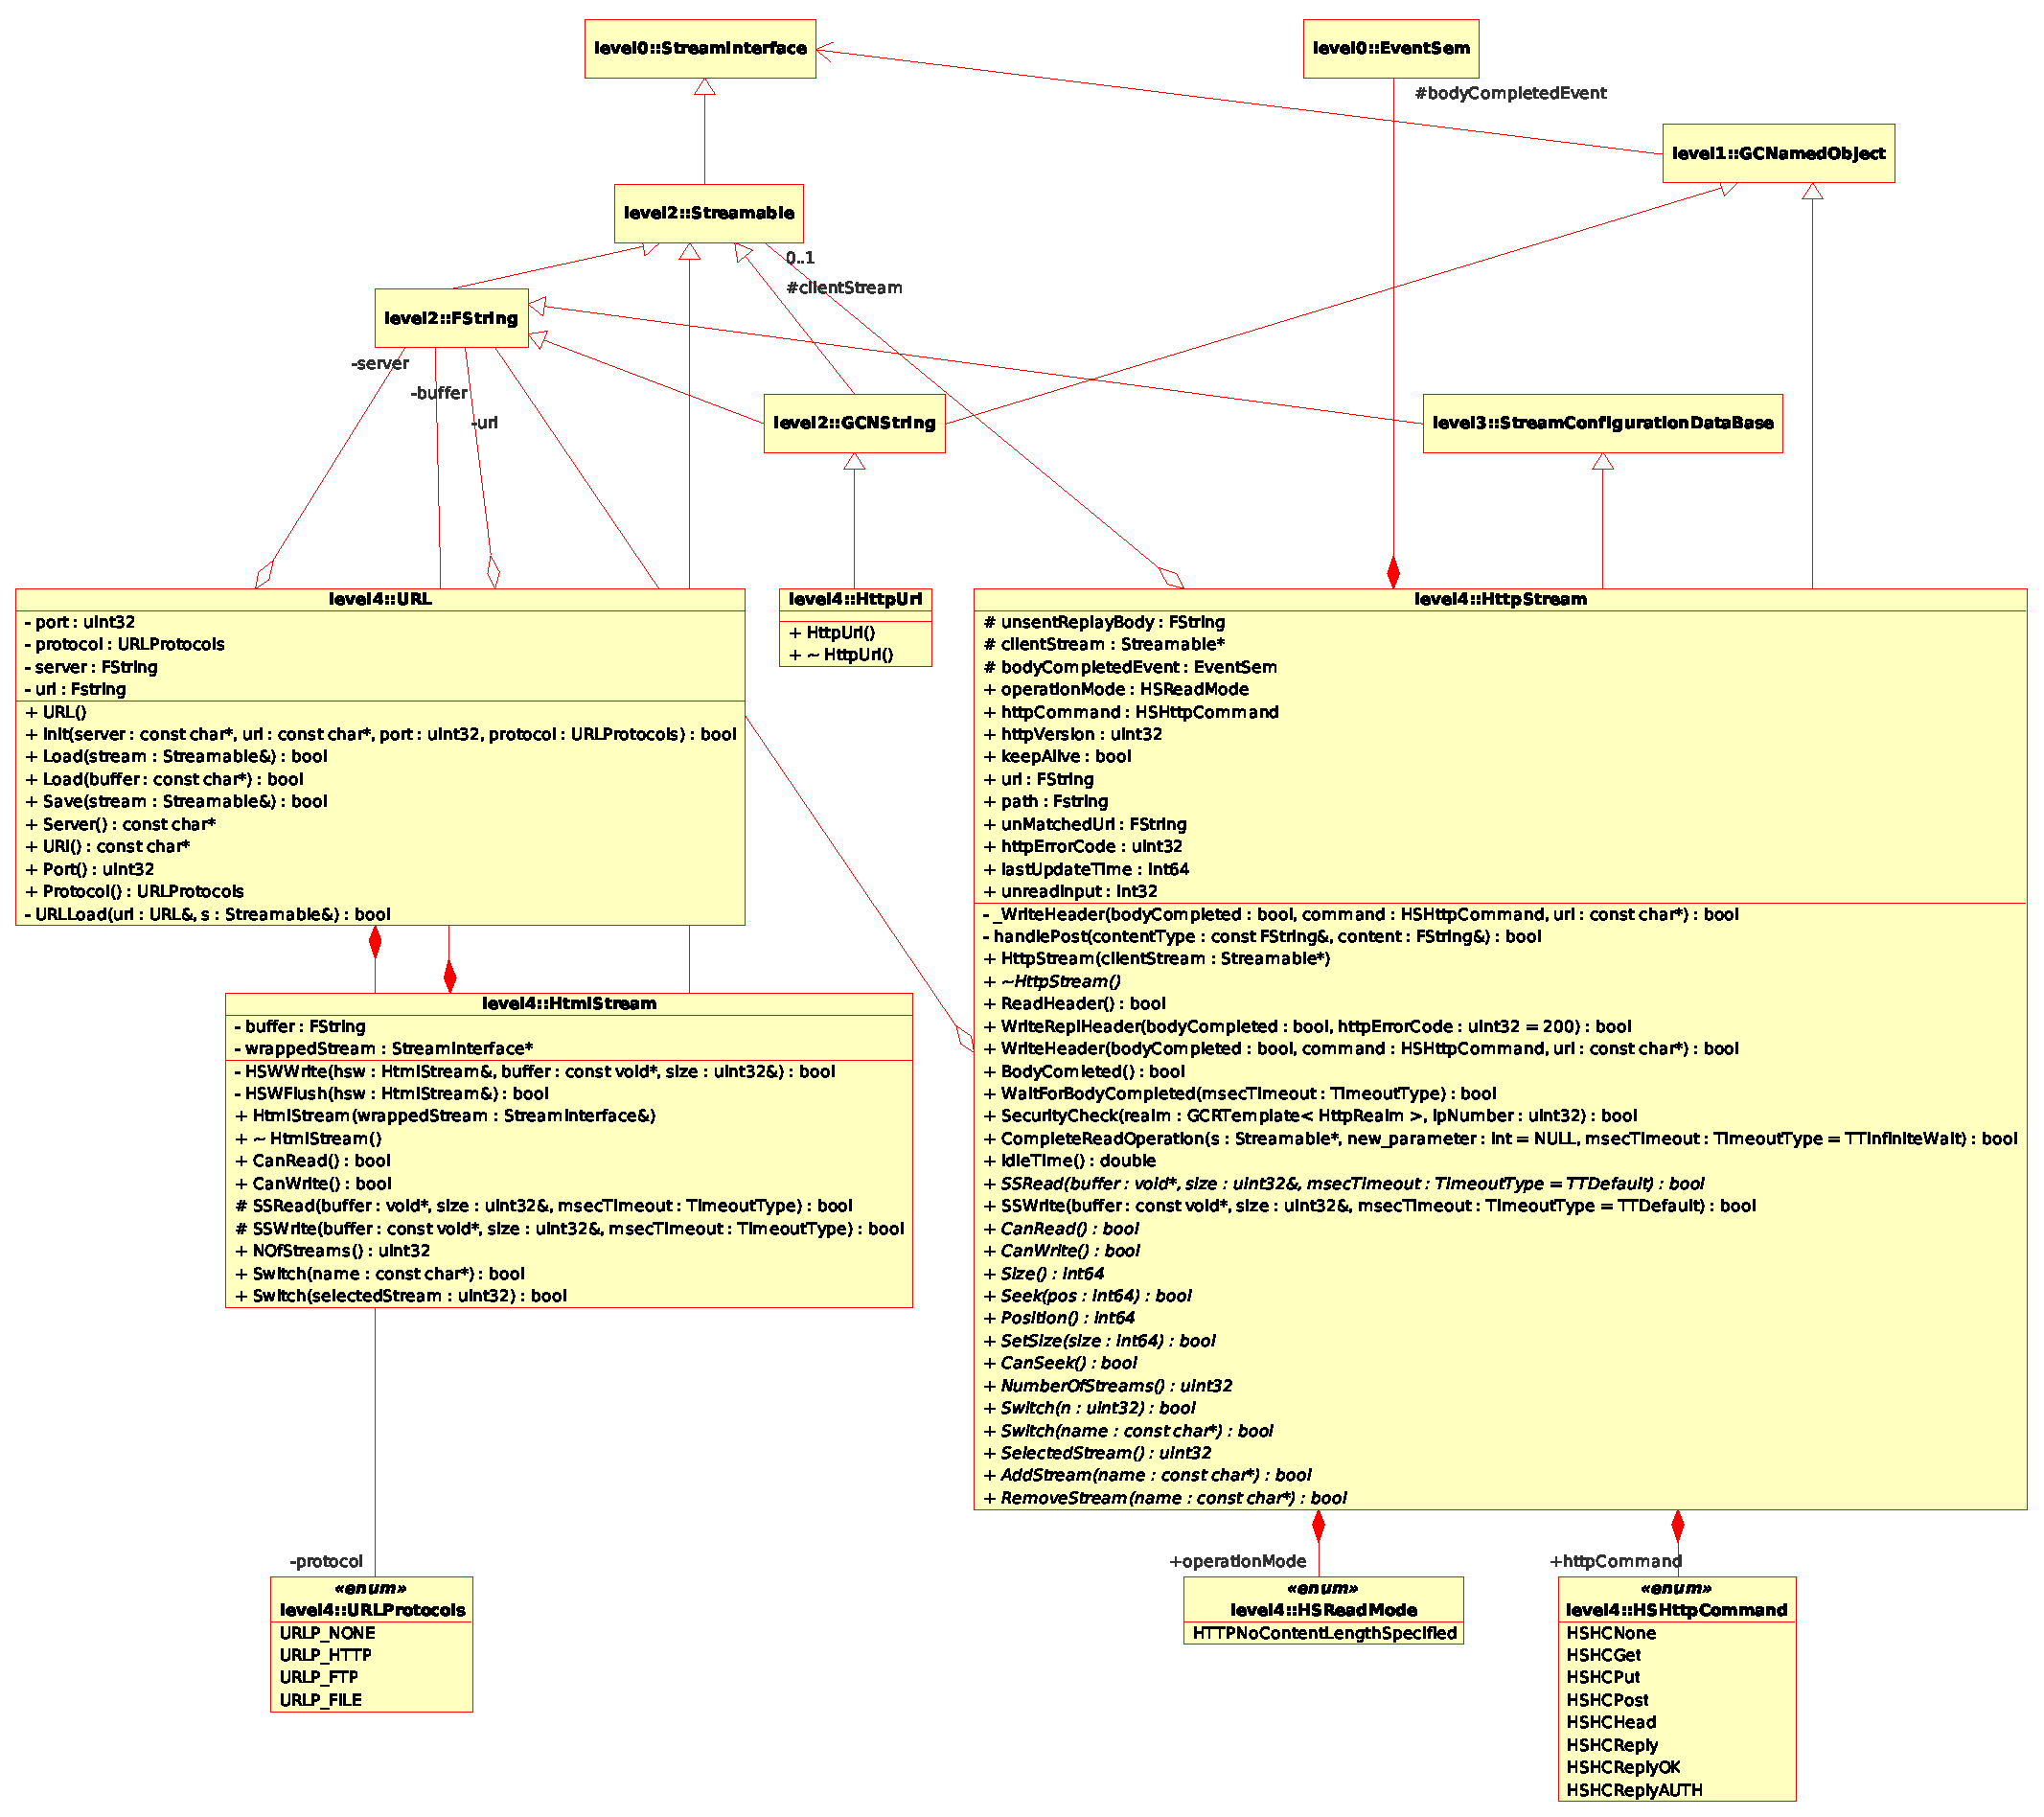
\includegraphics[width=\textwidth]{level4/level4-HttpStream.eps}
  \caption{BaseLib Level 4 HttpStream and URLs infrastructure}
  \label{f:level4:HttpStream}
 \end{center}
\end{figure}

Figure \ref{f:level4:HttpStream} depicts an UML schema of the classes involved in this section. Classes in this section are:
\begin{itemize}
 \item URL
 \item HttpURL

 \item HttpStream
 \item HtmlStream
\end{itemize}



\subsubsection{HttpStream}
\texttt{[HttpStream.h, HttpStream.cpp]}\\
The class \texttt{HttpStream} implements an HTTP language multiple stream. The main stream \textit{read} and \textit{write} channels, operate with the client (or on a cache until method \texttt{CompleteReadOperation} is not called); the other streams allow read/write access to special information like \texttt{HttpOptions} or HTML form commands.
The HTTP options are accessed using the streams whose name begins with \texttt{InputHttpOtions} or \texttt{OutputHttpOptions}. \texttt{InputCommands} contain the informations produced by submitting a form. The stream called \texttt{Peer} contains the name of the connecting peer.\\


The class \texttt{HttpStream} inherits from \texttt{GCNamedObject} and \texttt{StreamConfigurationDataBase}.
The first attribute, \texttt{unsentReplyBody}, is the part of the reply that is not sent yet; the second, \texttt{clientStream} is the stream connected to the remote client that should implement a timeout for read operation and translation for specific HTTP hex char groups; \texttt{bosyCompletedEvent} is a semaphore on which to wait for body completed.\\


Then come the public attributes. The attribute \texttt{operationMode} represents one of the following the values: \texttt{writeToString}, \texttt{writeToClient}, \texttt{writeToCDB}. The attribute \texttt{httpCommand} stores what command was requested; this affects the working of \texttt{Read} and \texttt{Write} methods, i.e. \texttt{Write} method on the main channel does not work for HTTP HEAD tag; it can also be the reply, in which case it contains the reply code. \texttt{httpVersion} holds the HTTP version number, i.e. \texttt{1000} means \textit{v1.0}, \texttt{2100} means \textit{v2.1}.
The attribute \texttt{keepAlive} is \texttt{true} if the communication should continue after transaction; the \texttt{url} is the URL of the requested page, the same information is also holded by the \texttt{path} attribute that store it with ``.'' (dotted notation) instead of ``\/''. \texttt{unMatchedUrl} stores the remainder of url not matched in the search. \texttt{httpErrorCode} sves the HTTP return code; the attribute \texttt{lastUpdateTime} is the last time the body has been updated and \texttt{unreadInput} is how much data is still waiting in the input stream from the client.
\begin{lstlisting}[
extendedchars=true,%
basicstyle=\fontfamily{pcr}\fontseries{m}\selectfont\footnotesize, %
stepnumber=1,%
numberstyle=\tiny,%
keywordstyle=\footnotesize\tt ,%
language=C++]
protected:
   FString unsentReplyBody;
   Streamable* clientStream;
   EventSem bodyCompletedEvent;
public:
   HSOperatingMode operationMode;
   HSHttpCommand httpCommand;
   uint32 httpVersion;
   bool keepAlive;
   FString url;
   FString path;
   FString unMatchedUrl;
   uint32 httpErrorCode;
   int64 lastUpdateTime;
   int32 unreadInput;
\end{lstlisting}


The method \texttt{handlePost} handles a post request. The constructor builds an empty class, and the destructor simply destroies it.


The method \texttt{ReadHeader} reads the HTTP header and leaves body up to the user; \texttt{WriteReplyHeader} begins an HTTP reply message: sends out the HTTP header as currently formed and the outstanding body; any further write will operate directly on the stream; if \texttt{complete} is \texttt{true} then the whole body has been cached and therefore we can announce the body size. \texttt{WriteHeader} begins an HTTP message: sends out the HTTP header as currently formed and the outstanding body; any further write will operate directly on the stream if complete is \texttt{true} then the whole body has been cached and therefore we can announce the body size, if \texttt{command} is a reply we are generating a reply message.\\


The method \texttt{BodyCompleted} returns \texttt{true} if the writing of the body has been completed. \texttt{WaitForbodyCompleted} is a sender thread that waits for the completion of this activity.


The method \texttt{SecurityCheck} checks a request against a security module; \texttt{CompleteReadOperation} completes the reading of an HTTP message throwing away the content. \texttt{IdeleTime} returns how long since the last write operation.
\begin{lstlisting}[
extendedchars=true,%
basicstyle=\fontfamily{pcr}\fontseries{m}\selectfont\footnotesize, %
stepnumber=1,%
numberstyle=\tiny,%
keywordstyle=\footnotesize\tt ,%
language=C++]
   bool _WriteHeader(bool bodyCompleted,HSHttpCommand command,const char* url);
private:
   bool handlePost(const FString& contentType, FString& content);
public:
   HttpStream(Streamable *clientStream);
   virtual ~HttpStream();

   bool ReadHeader();
   bool WriteReplyHeader(bool bodyCompleted,uint32 httpErrorCode=200);
   inline bool WriteHeader(bool bodyCompleted,HSHttpCommand command,const char* url);

   bool BodyCompleted();
   bool WaitForBodyCompleted(TimeoutType msecTimeout);

   bool SecurityCheck(GCRTemplate<HttpRealm> realm,uint32 ipNumber);
   bool CompleteReadOperation(Streamable* s=NULL,TimeoutType msecTimeout=TTInfiniteWait);
   double IdleTime();
\end{lstlisting}

Other methods, that follow, override the \texttt{Streamable} ones, we report them for a documnentation purpose.

\begin{lstlisting}[
extendedchars=true,%
basicstyle=\fontfamily{pcr}\fontseries{m}\selectfont\footnotesize, %
stepnumber=1,%
numberstyle=\tiny,%
keywordstyle=\footnotesize\tt ,%
language=C++]
   virtual bool SSRead(void* buffer,uint32& size,TimeoutType msecTimeout=TTDefault);
   virtual bool SSWrite(const void* buffer,uint32& size,TimeoutType msecTimeout=TTDefault);
   virtual bool CanRead();
   virtual bool CanWrite();

   virtual int64 Size();
   virtual bool Seek(int64 pos);
   virtual bool CanSeek();
   virtual int64 Position();
   virtual bool SetSize(int64 size);

   virtual uint32 NumberOfStreams();
   virtual bool Switch(uint32 n);
   virtual bool Switch(const char* name);
   virtual uint32 SelectedStream();
   virtual bool AddStream(const char* name);
   virtual bool RemoveStream(const char* name);
\end{lstlisting}



\section{HttpInterface and HttpRealm}


\begin{figure}[h!]
 \begin{center}
  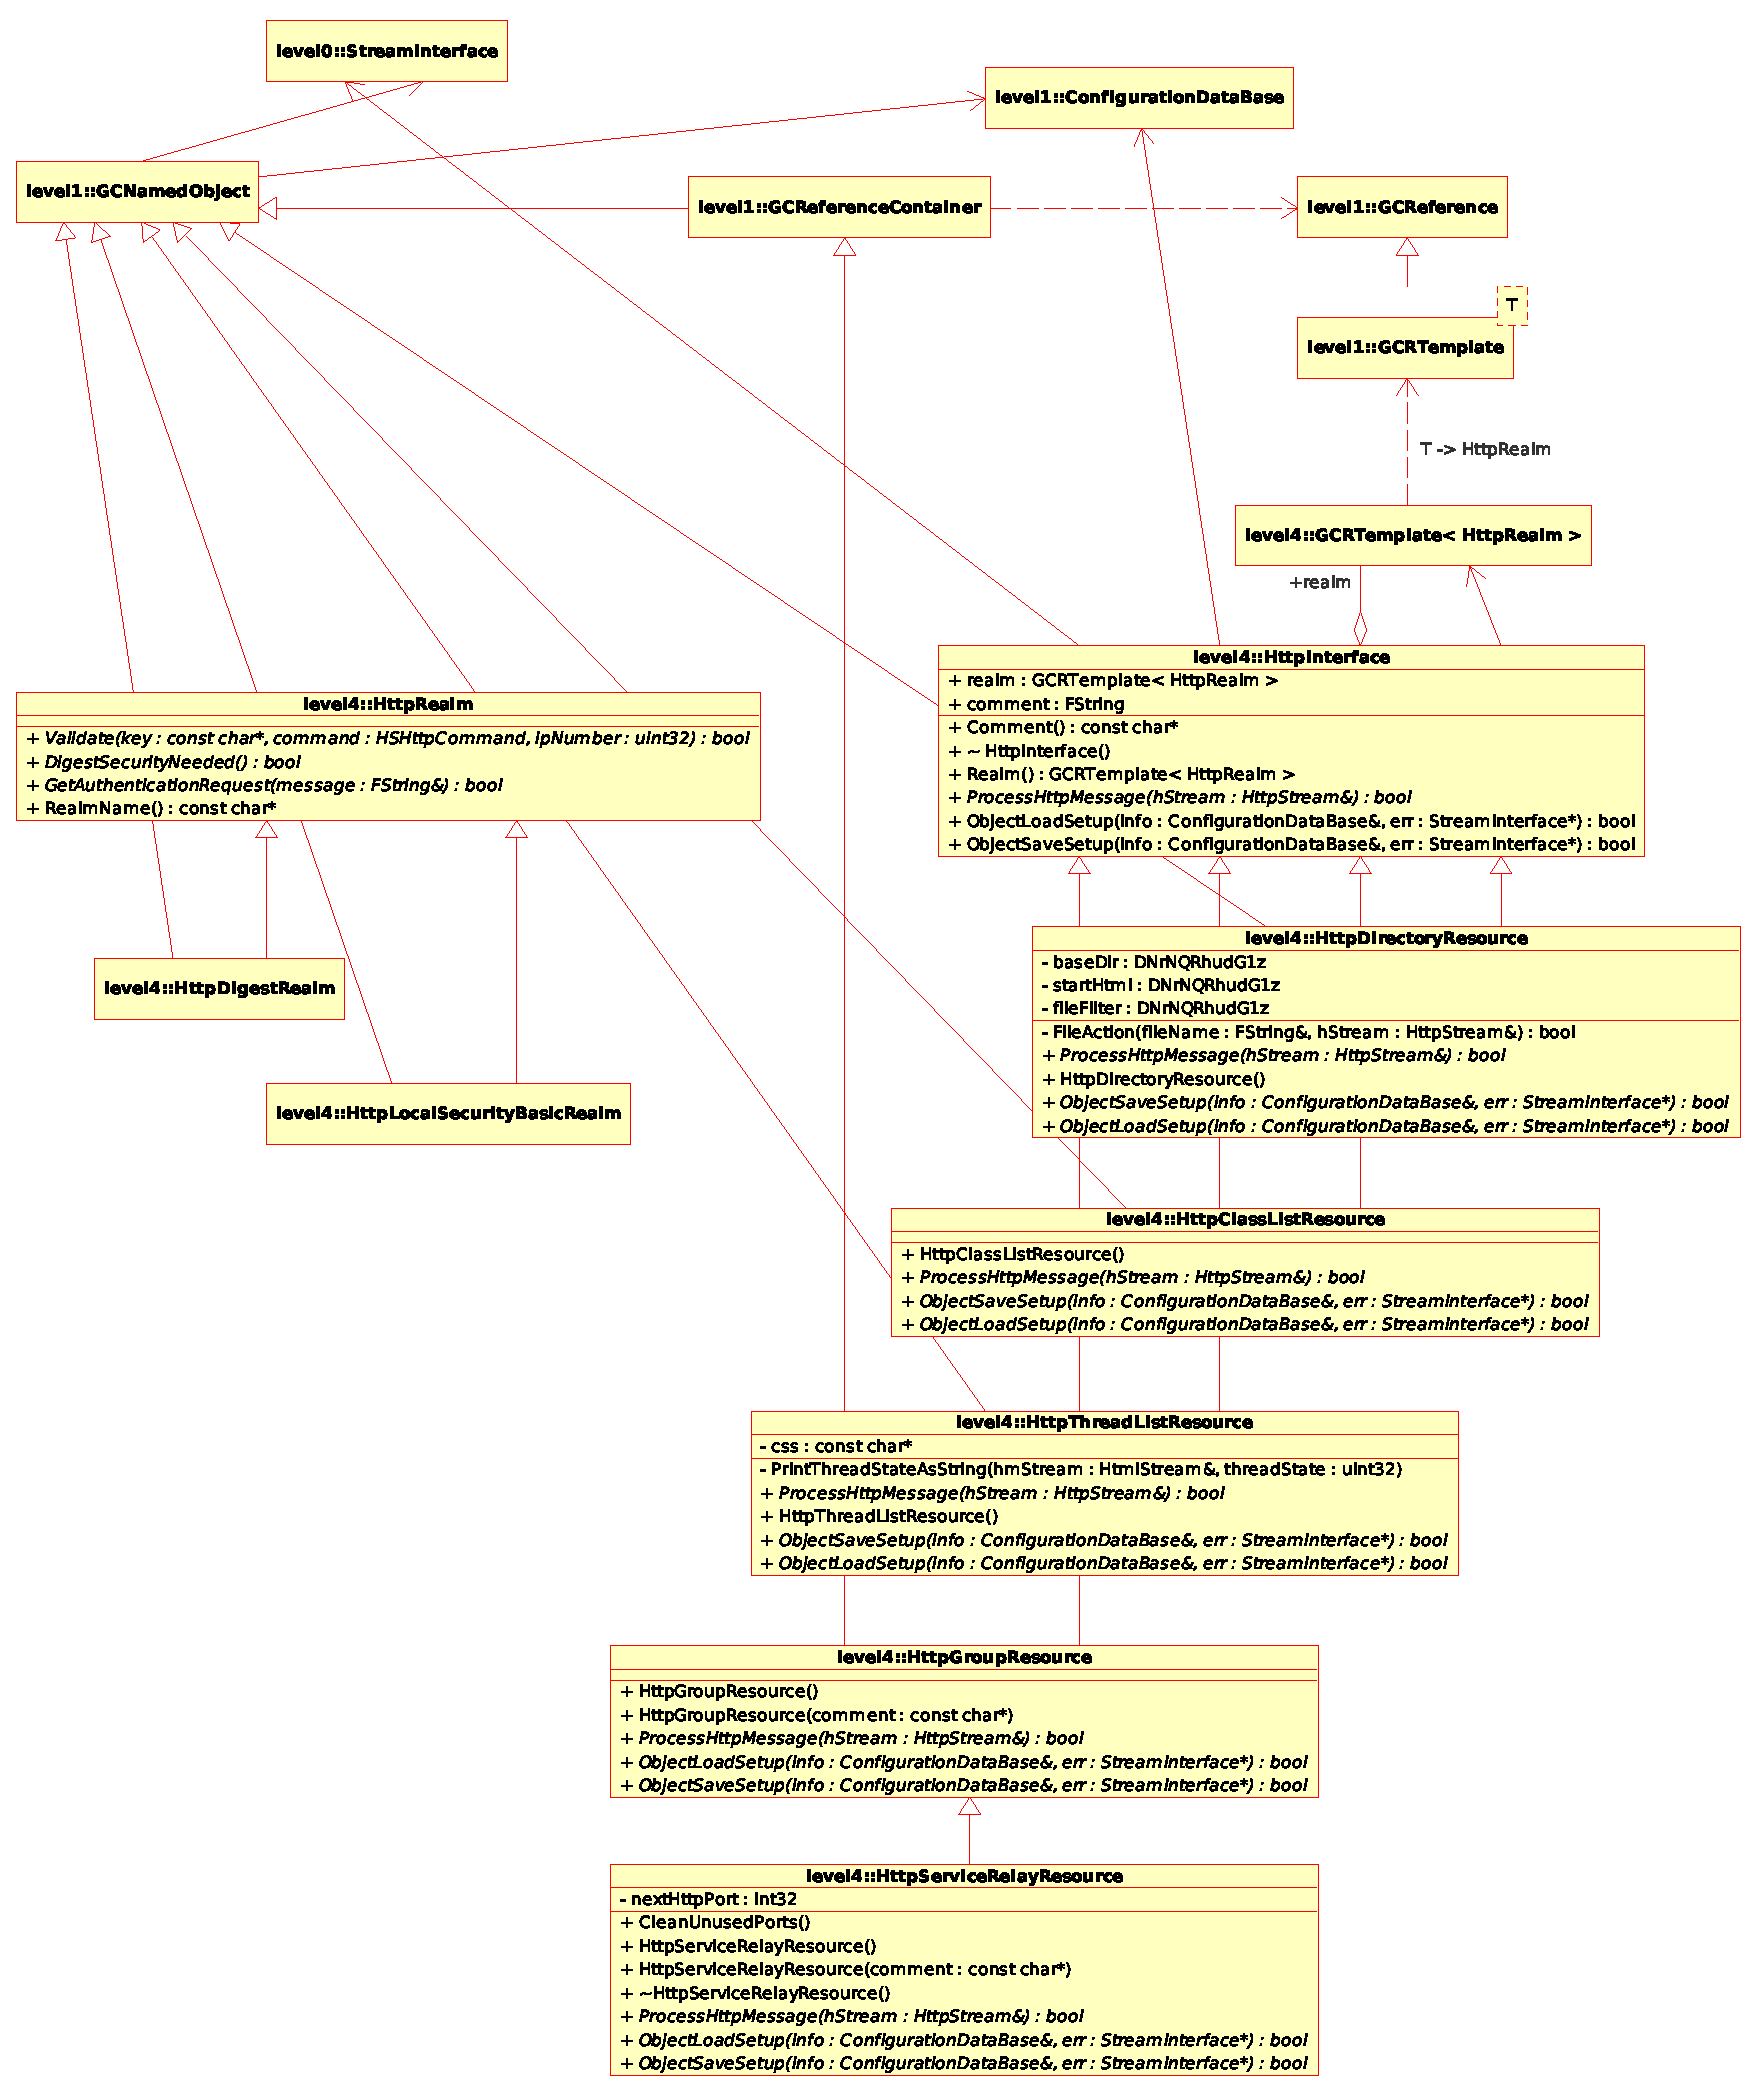
\includegraphics[width=0.88\textwidth]{level4/level4-HttpInterface.eps}
  \caption{BaseLib Level 4 HttpInterface and HttpRealm}
  \label{f:level4:HttpInterface}
 \end{center}
\end{figure}

Figure \ref{f:level4:HttpInterface} depict an UML diagram of classes in this section. Classes in this section are (the first three are from the security suite and the others comes from the \texttt{HttpInterface} hierarchy):
\begin{itemize}
 \item HttpRealm
 \item HttpDigestRealm
 \item HttpLocalSecurityBasicRealm

 \item HttpInterface
 \item HttpDirectoryResource
 \item HttpClassListResource
 \item HttpThreadListResoource
 \item HttpGroupResource
 \item HttpService RelayResource
\end{itemize}



\subsubsection{HttpInterface}
\texttt{[HttpInterface.h]}\\
The class \texttt{HttpInterface} is the base class for a generic HTTP resource object; each resource object that wants to share its state or part of its state via the BaseLib HTTP server must inherits this interface and overriddes the \texttt{ProcessHttpMessage} method.

In the overridden \texttt{ProcessHttpMessage} the subclass must output an HTTP page about the state of the class.\\


The method \texttt{GCRTemplate<HttpRealm>} is a reference to the \textit{realm} database, i.e. a container of security options; \texttt{comment} is the page name to be presented to the viewer.


The method \texttt{Comment} return \texttt{comment.Buffer()}; \texttt{Realm} method return a reference to the \texttt{realm} database. The method \texttt{ProcessHttpMessage} is the method that will be overridden to obtain an HTTP page for the subclassed object.

The method \texttt{ObjectLoadSetup} calls \texttt{realm}'s one that is inherited from the \texttt{GCRTemplate}; the method \texttt{ObjectSaveSetup} behave the same as \texttt{ObjectLoadSetup}.

\begin{lstlisting}[
extendedchars=true,%
basicstyle=\fontfamily{pcr}\fontseries{m}\selectfont\footnotesize, %
stepnumber=1,%
numberstyle=\tiny,%
keywordstyle=\footnotesize\tt ,%
language=C++]
public:
   GCRTemplate<HttpRealm> realm;
   FString comment;

public:
   virtual ~HttpInterface(){};
   const char* Comment();
   GCRTemplate<HttpRealm> Realm();
   virtual bool ProcessHttpMessage(HttpStream& hStream)=0;
   bool ObjectLoadSetup(ConfigurationDataBase& info,StreamInterface* err);
   bool ObjectSaveSetup(ConfigurationDataBase& info,StreamInterface* err);
\end{lstlisting}



\chapter{BaseLib Level 5}
\chaptermark{Level 5}

BaseLib Level 5 deals about different software mechanisms that makes components communicate and execute. The first presented mechanism is the \textit{Object's Message Passing}, it is infact possible to send and receive messages between objects, we are used to ear about messages between threads or processes, in BaseLib this concept goes much further and arrive to objects (i.e. a thread its an object in BaseLib). There is a further extension to the \textit{Object's Message Passing} that let's the user manipulate also HTTP messages.

A second really usefull mechanism is the \textit{State Machine}, i.e. the possibility to define and easily create a state machine in a similar fashion of Matlab StateFlow. Each flavour of state machine can be created.

A signal of data can be completely described by the \textit{Signal} class and many signals are packed togheter, by the access mode, to form an \textit{Interface}, more then one interface form a \textit{Generic Application Module} (a GAM). A GAM can be thinked as a Matlab Simulink computational block. A set of blocks communicate between them using a memory buffer, this memory buffer is provided by the Dynamic Data Buffer (DDB).
The last mechanism offered by this level are the \textit{Menu}. \\

Follow a list of the sections in this chapter:
\begin{itemize}
 \item Messages
 \item HTTP Messages

 \item State Machine

 \item Signals
 \item DDB, GAM

 \item Menu
 \item Others
\end{itemize}



\section{Messages}

This section introduces the object message passing infrastructure of BaseLib. This is another powerfull subsystem that let you send messages between different objects instances locally and on remote systems (using the UDP/IP protocol). To send remotely a message serializiation and deserialization, seen in the previous chapters, is exploited. Point to point messages and multicast messages are supported. Mainly messages are asynchronous but early and late replay can be sended so synchronous messages can also be created. Summarizing, messages can be:
\begin{itemize}
 \item local, remote \textit{send}
 \item point to point, multicast messages (\textit{multiple destinations})
 \item immediate, delayed \textit{dispatching}
 \item early, late \textit{replay} (also acknowledge)
\end{itemize}

Figure \ref{f:level5:MSGprop} try to graph the properties that a message can have and the dependencies between those properties. For example an immediate message doesn't answer to an early replay.

\begin{figure}[h!]
 \begin{center}
  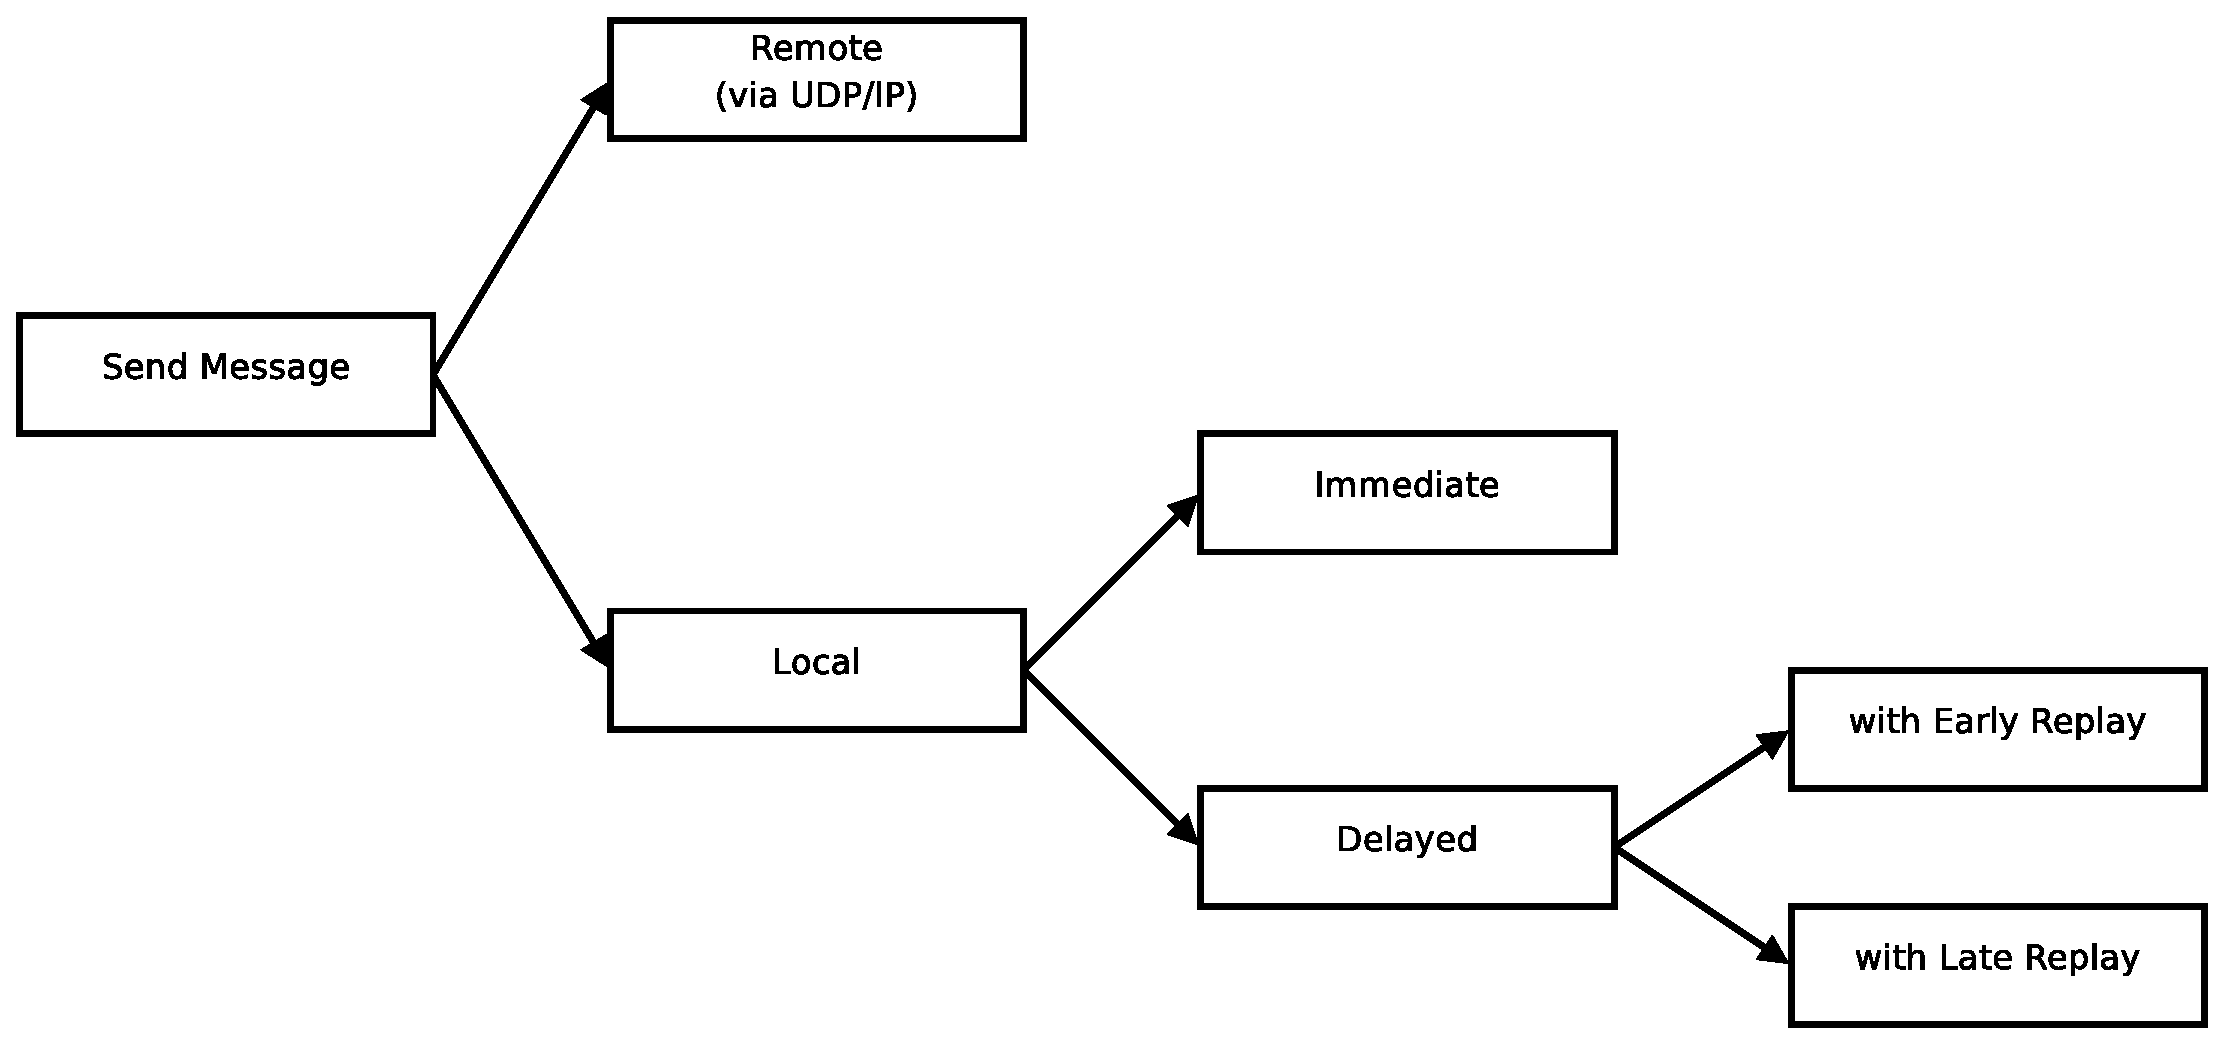
\includegraphics[width=0.66\textwidth]{level5/MessagesProp.eps} 
  \caption{BaseLib Level 5 messages properties diagram}
  \label{f:level5:MSGprop}
 \end{center}
\end{figure}


Using UDP/IP the policy for remote messages handling is to be Real Time, if it arrives it's ok otherwise doesn't mind, the timeout will save you.

Every message can be build up of any object type, a message is a list of objects that can also be a message itself. The whole UML diagram is depicted in Figure \ref{f:level5:MSG} and classes involved in this section are:
\begin{itemize}
 \item MessageCode
 \item Message

 \item MessageQueue
 \item MessageInterface
 \item MessageHandler

 \item MDRFlags
 \item MessageEnvelope
 \item MessageDeliveryRequest

 \item MessageDispatcher
 \item MessageBroker
 \item StartStopMessageHandlerInterface
 \item MessageServer
\end{itemize}

A \texttt{MessageCode} is an integer code that let comparing messages on the base of it; otherwise a message can be distingued from a string that is holded by the \texttt{Message} class.

Basically the vital work is done by the \texttt{MessageHandler} class that depends by the \texttt{MessageQueue} that holds messages that can be dispatched not immediately and by the \texttt{MessageInterface} that require the implementation of the two processing methods for the messages. \\
\begin{figure}[h!]
 \begin{center}
  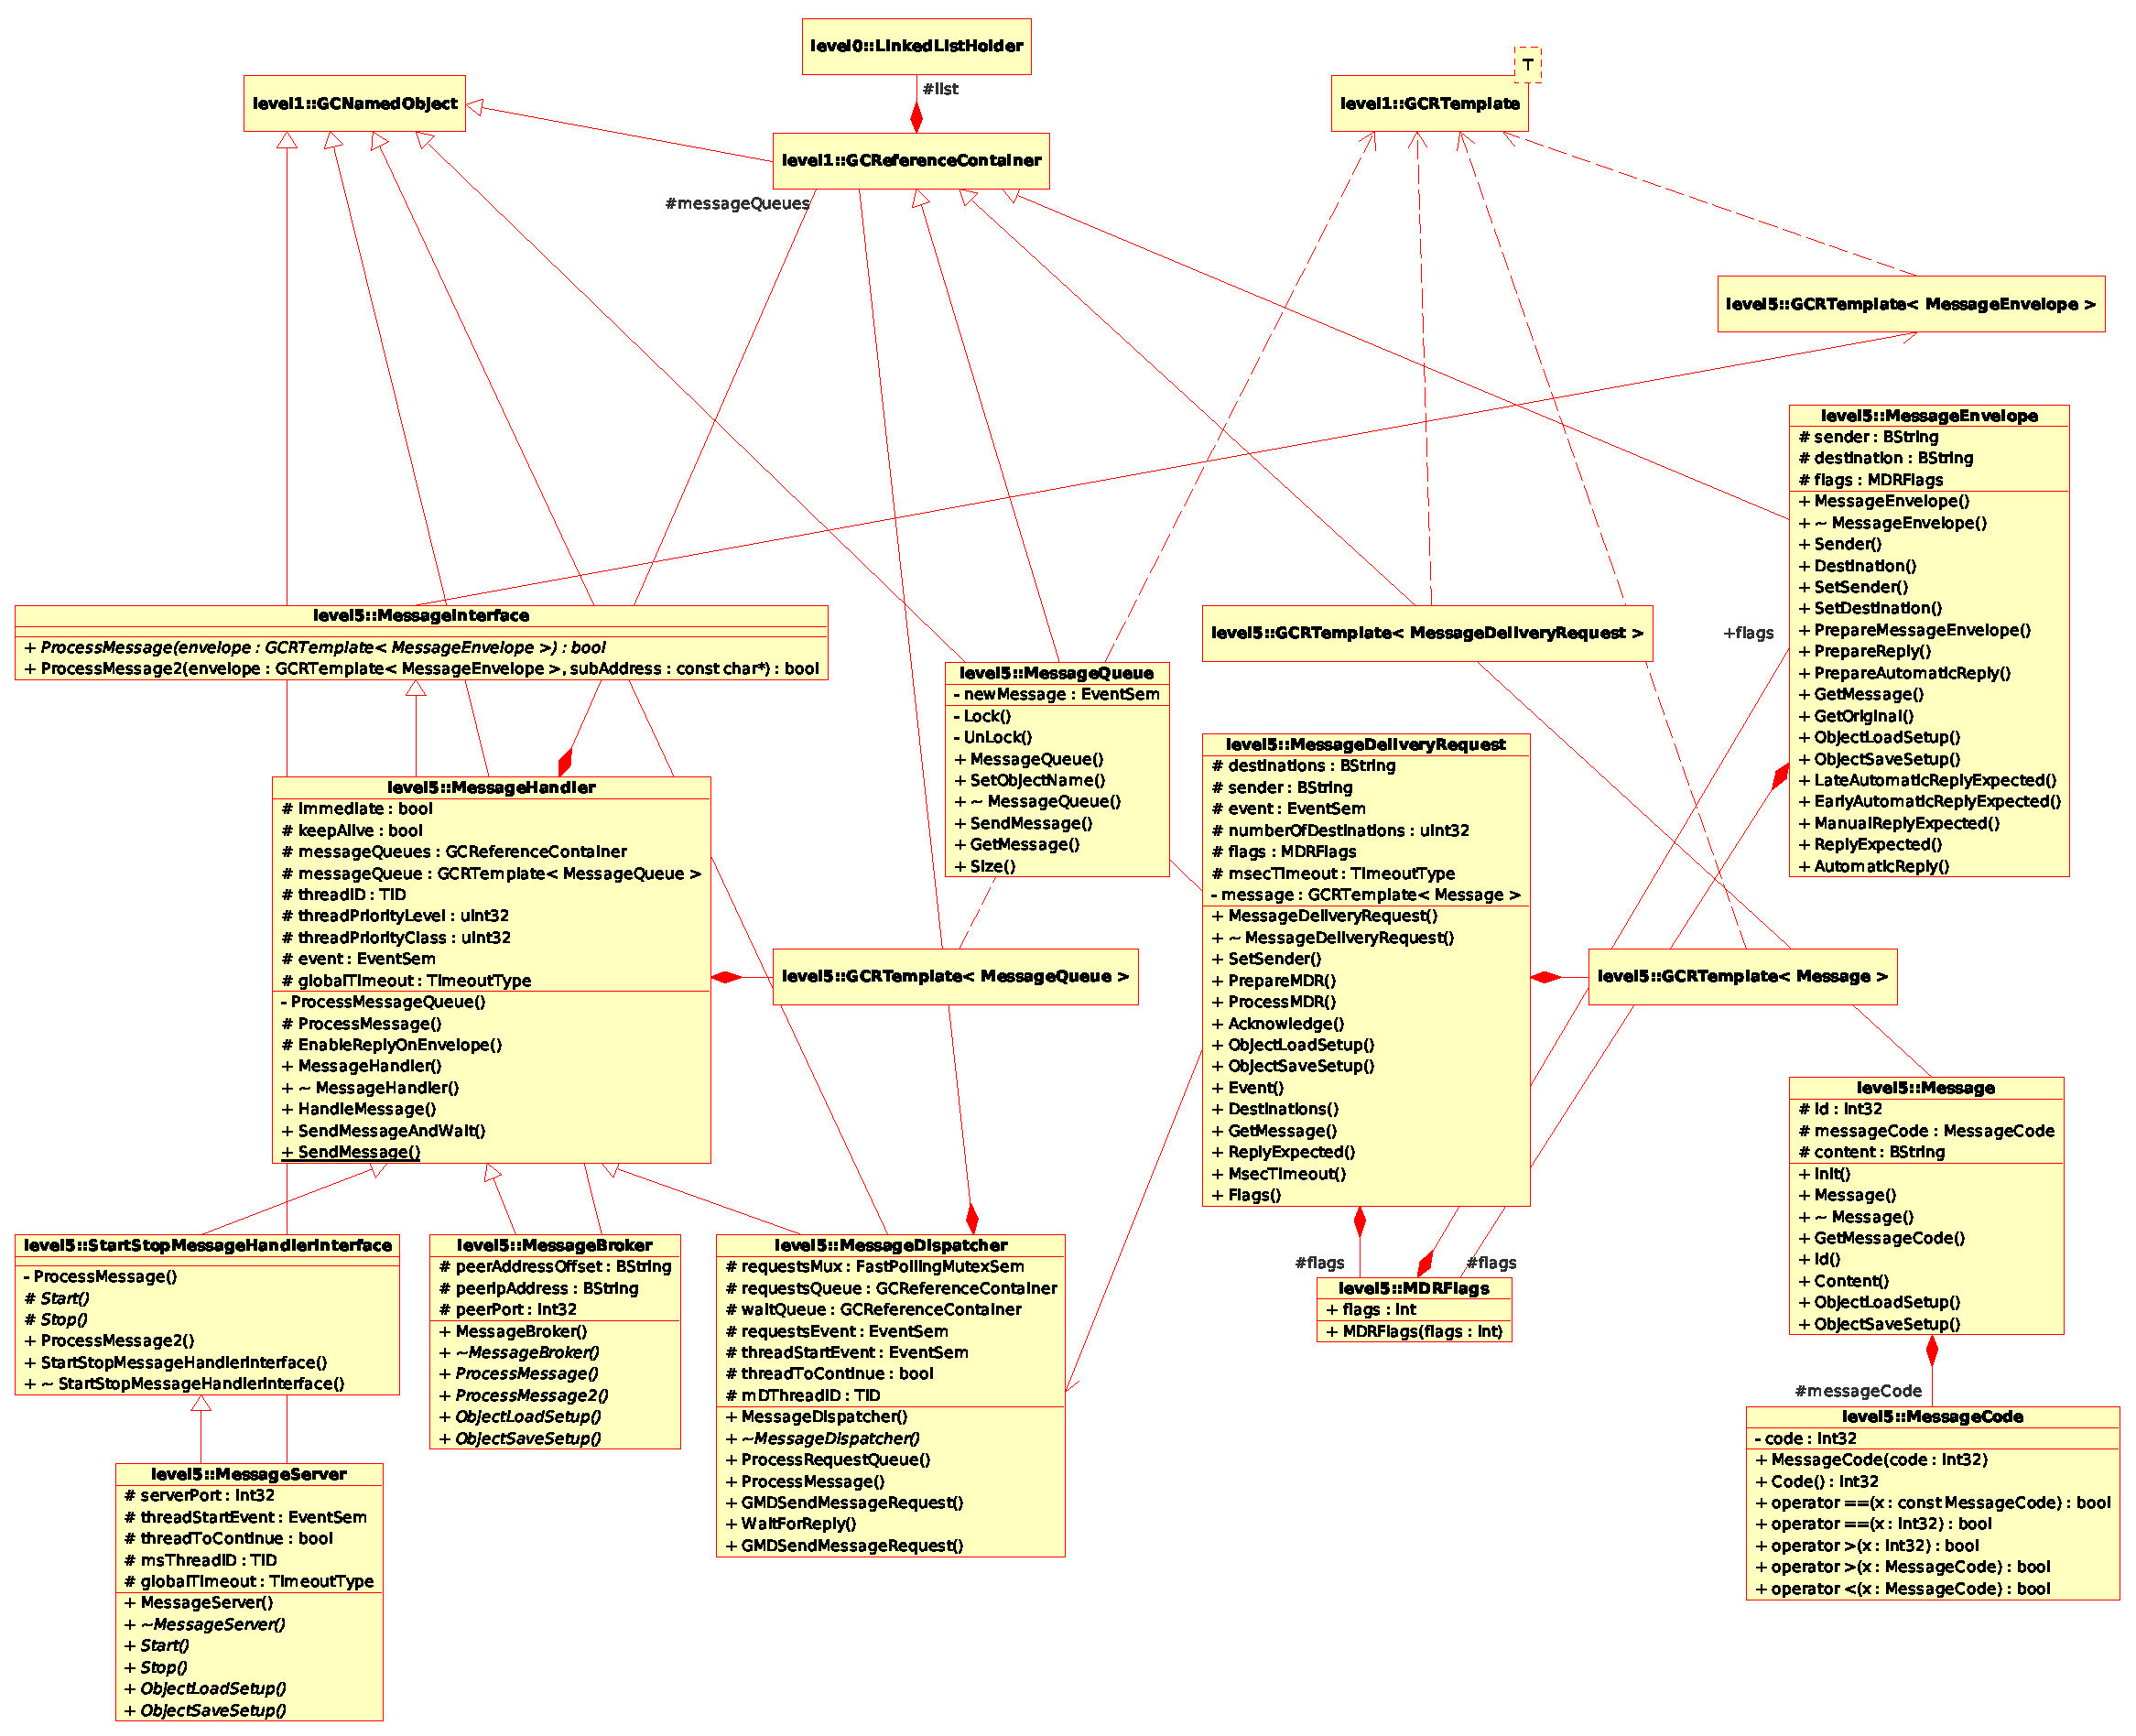
\includegraphics[width=1.1\textwidth]{level5/level5-MSG-exp.eps} 
  \caption{BaseLib Level 5 Messages}
  \label{f:level5:MSG}
 \end{center}
\end{figure}

The main method to send messages is the static \texttt{MessageHandler::SendMessage()}. This method is static so it is freely callable by any other classes that doesn't know how to send; if a class need a reply must extends the class \texttt{MessageHandler} or one of its subclasses. Any class that is a destination of a message must extend \texttt{MessageHandler}, and like before, or one of its subclasses. \\


Figure \ref{f:level5:MSG-dispatch} is an UML activity diagram that depict the steps for sending a message thorught the message infrastructure; some comments are needed. To send a message, the message must be first created, so a new \texttt{Message} class must be instantiated and a \texttt{MessageEnvelope} must be setted up with the source object pointer and the name of the destination class; the final destination class must be a \texttt{MessageHandler} subclass, otherwise it can not receive the message. We write ``final destination class'' because a destiantion address can be a dotted separated address of class names, i.e. the message can be sended between classes in a serial way, this is usefull for example in cases when you need to communicate to a remote class in another machine. An example of a remote location can be ``messageBroker.synchronizationGAM'' or ``(@192.168.2.3:1234).synchronizationGAM''. \\


After creating a \texttt{MessageEnvelope} it is possible to send it via the static \texttt{SendMessage} method; the first thing that is done is to check if it is a valid object, then the address is checked to know if it is a remote or a local message. If it is a remote message the \texttt{Message} is serialized and an UDP/IP socket is opened and the serialized object is sended.

If the message is local the first things that is done is to check against existance of the receiver object, if it exists in the GODB (the global registry of objects), it will be checked if it is of type \texttt{MessageHandler} otherwise the function returns with an error, infact if the receiver is not a \texttt{MessageHandler} subclass the message can not be delivered furthermore.

If the classes is founded then the control of the message is passed to class's methods, the first thing is to check against the form of dispatching, if it is \textit{immediate} the class's \texttt{ProcessMessage2} is called, otherwise a detached thread is made running and the message is queued for dispatching and the method returns.

\begin{sidewaysfigure}[h!]
 \centering
 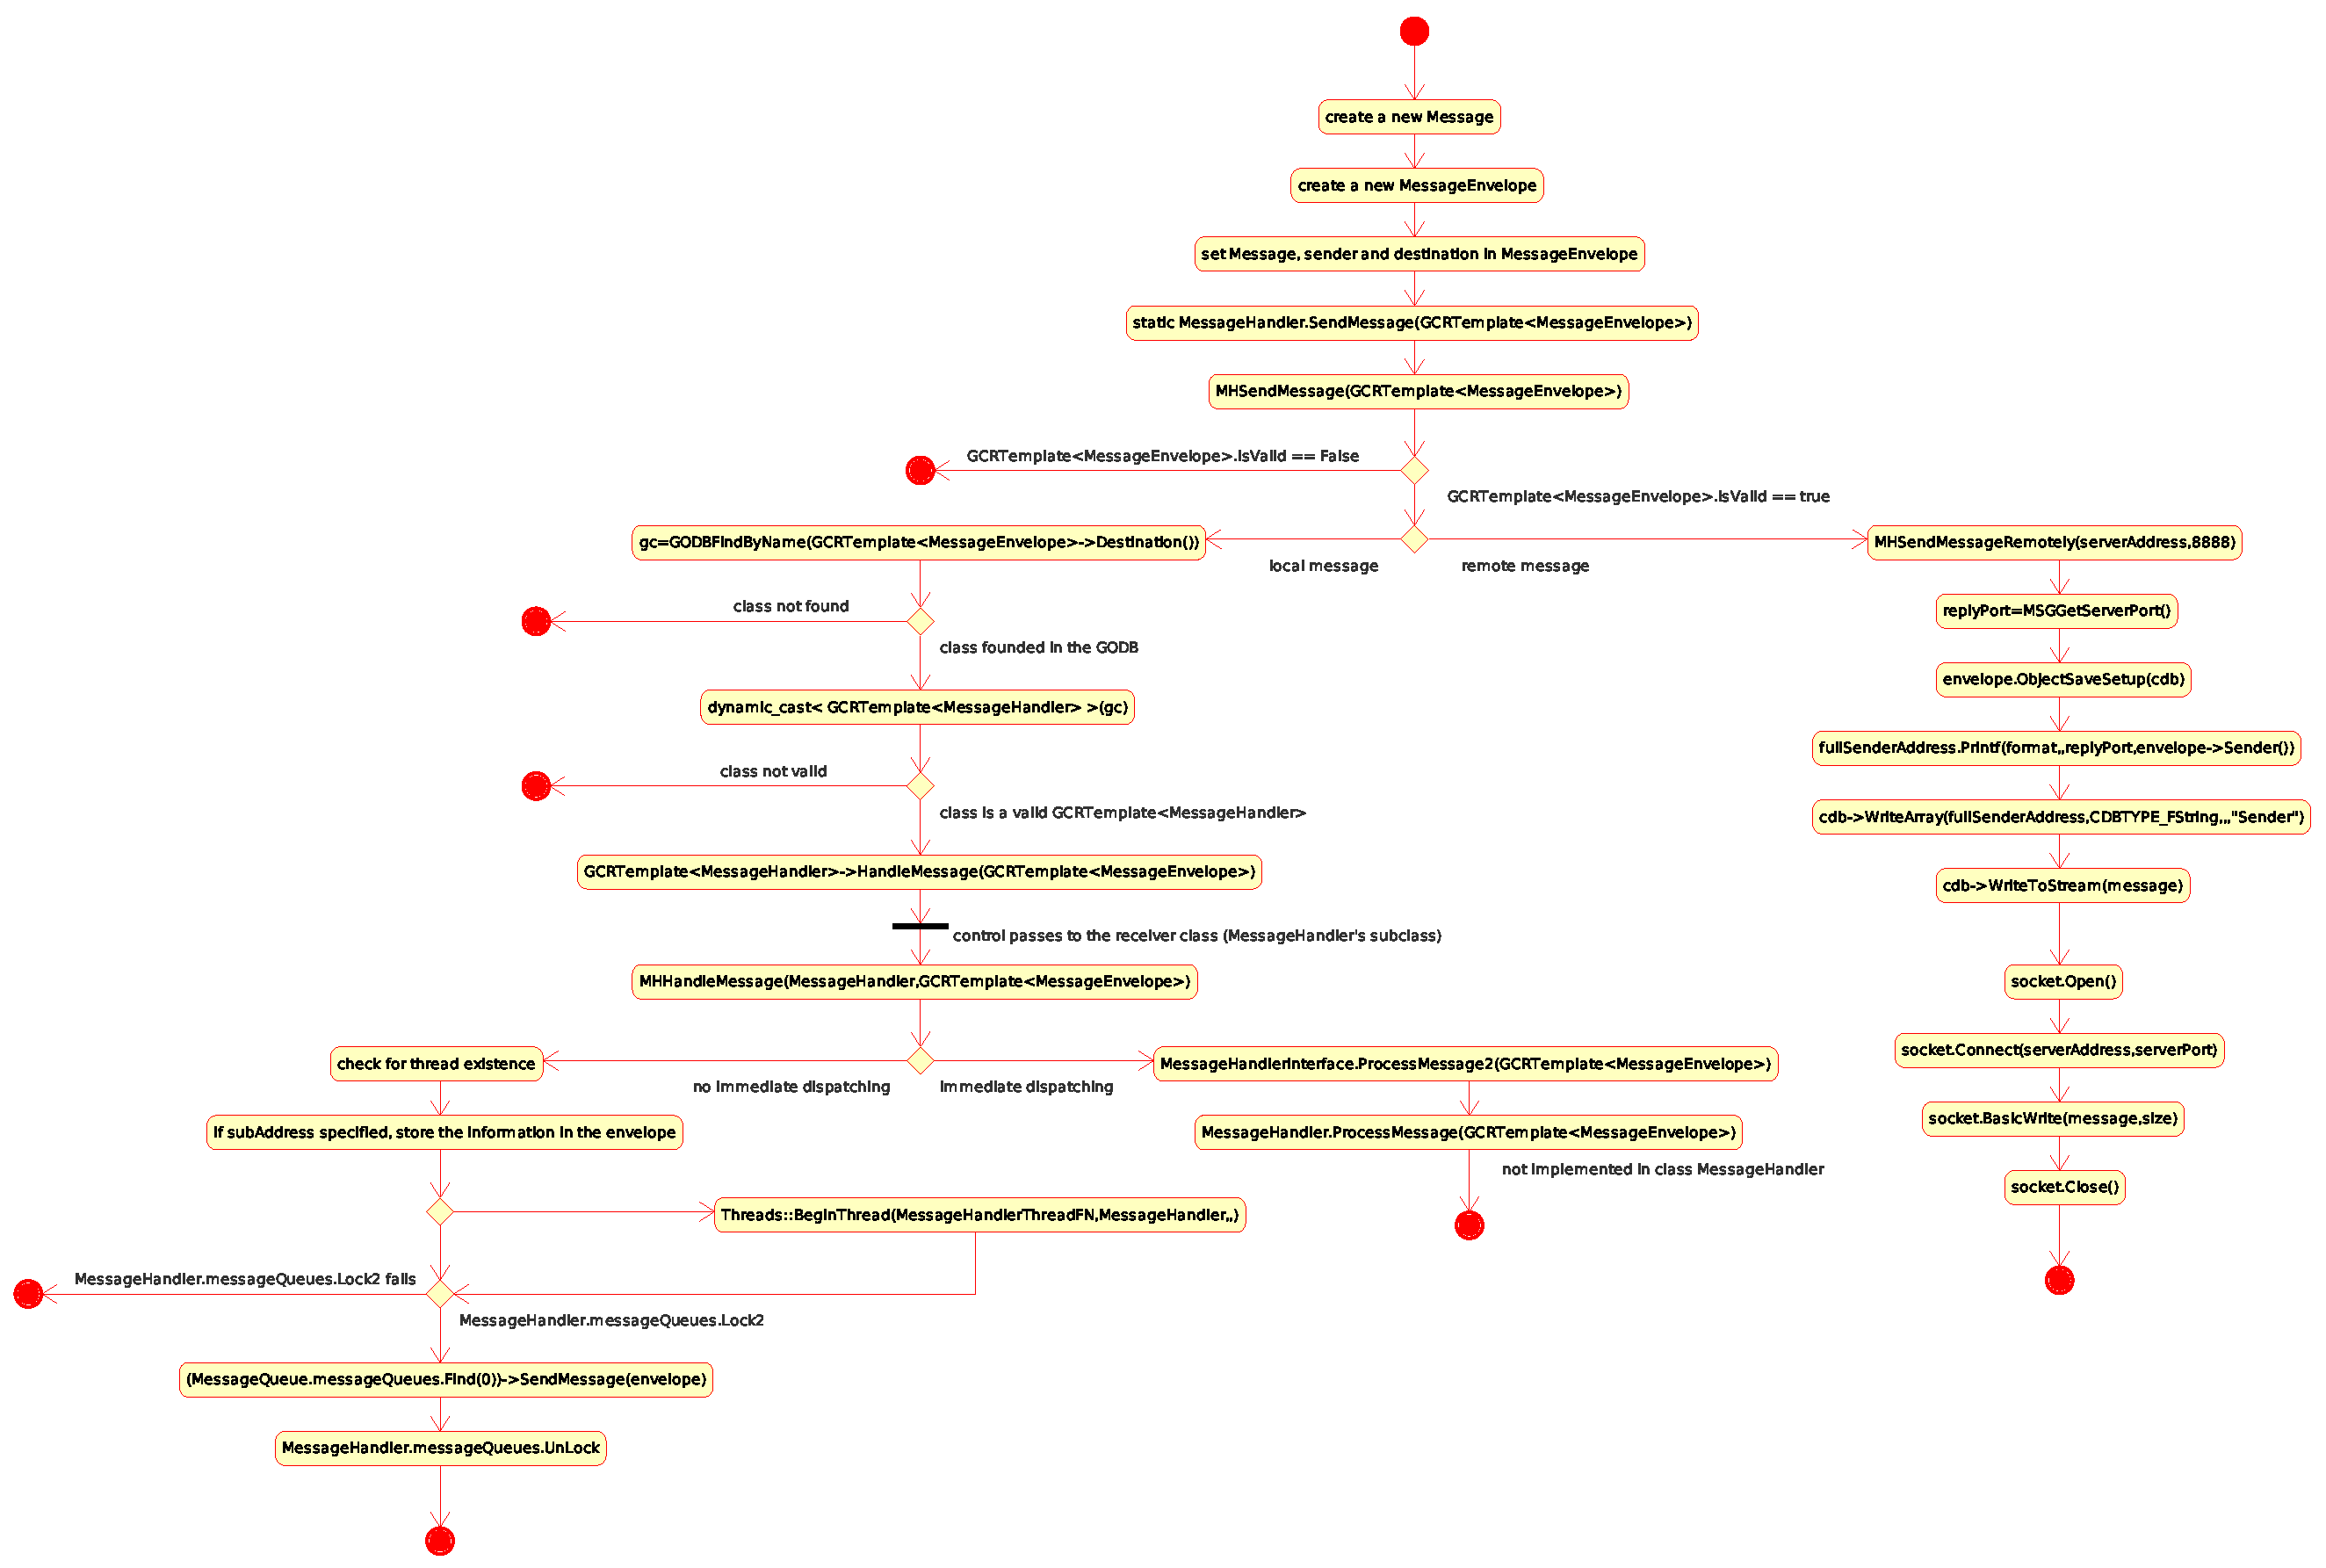
\includegraphics[width=\textwidth]{level5/MSG-dispatching.eps}
 \caption{BaseLib Level 5 \texttt{static MessageHandler::SendMessage()}}
 \label{f:level5:MSG-dispatch}
\end{sidewaysfigure}
\clearpage



The detached thread is a \texttt{MessageHandlerThreadFN}, refer to Figure \ref{f:level5:MSG-ThreadFN}, this thread is an asynchronous entity that delivers messages queued on the object. For each message an early reply and a late reply can be requested, the early reply is a message sended before the action of calling the \texttt{ProcessMessage2} method and the late reply after. There is a special treatment for \texttt{MenuMessage}s.

\begin{figure}[h!]
 \begin{center}
  \includegraphics[width=0.77\textwidth]{level5/MSG-ThreadFN.eps} 
  \caption{BaseLib Level 5 \texttt{MessageHandlerThreadFN}}
  \label{f:level5:MSG-ThreadFN}
 \end{center}
\end{figure}



\subsubsection{MessageCode}
\texttt{[MessageCode.h]}\\
The class \texttt{MessageCode} implements the codes of the messages and some already defined codes. Such class is used to describe the content of a message, is just an integer but it enforces type checks. User defined \texttt{MessageCode}s starts from \texttt{UserMessageCode} (defined in the following). \\


As before the unique attribute is an \texttt{int32} that define the code itself. The constructor creates a new \texttt{MessageCode} object with the code passed by argument. \texttt{Code} accesses the \texttt{code} attribute. Then a set of operator redefinitions comes that are able to compare between message codes.
\begin{lstlisting}[
extendedchars=true,%
basicstyle=\fontfamily{pcr}\fontseries{m}\selectfont\footnotesize, %
stepnumber=1,%
numberstyle=\tiny,%
keywordstyle=\footnotesize\tt ,%
language=C++]
private:
   int32 code;

public:
   MessageCode(int32 code);
   inline int32 Code() const;

   inline bool operator==(const MessageCode x) const;
   inline bool operator==(int32 x) const;
   inline bool operator>(int32 x) const;
   inline bool operator>(MessageCode x) const;
   inline bool operator<(MessageCode x) const
\end{lstlisting}

The following message codes are statically defined in the \textit{level5/MessageCode.h} file. Each file that include \textit{MessageCode.h} has a local copy of these objects. Is a waste of space.

\begin{table}[!h]
 \begin{center}
  \begin{tabular}{|l|l|l|}
   \hline
description & object name & \texttt{int32 code} \\
    \hline
message rejected by the original recipient & \texttt{RejectedMessage} & \texttt{0xFFFFFFFF} \\
used when there is nothing to say & \texttt{NullMessage} & \texttt{0x0000} \\
standard reply to fully acknowledge a message & \texttt{FinishedMessage} & \texttt{0x0001} \\
a message directed to a \texttt{MenuInterface} & \texttt{MenuMessage} & \texttt{0x1001} \\
a message directed to a \texttt{HttpInterface} & \texttt{HttpMessage} & \texttt{0x1002} \\
first user defined message & \texttt{UserMessageCode} & \texttt{0x100000} \\
how many user message codes & \texttt{MaxUserMessageCode} & \texttt{0x100000} \\
    \hline
    \end{tabular}
   \end{center}
  \caption{Level5 Message codes}
 \label{t:level5:MSGCode}
\end{table}

\texttt{RejectedMessage} is the result of a message rejected by the original recipient; \texttt{NullMessage} is an empty message used when there is nothing to say; \texttt{FinishedMessage} is returned when it has finished using the data in the original message, this is the standard reply to fully acknowledge a message. \texttt{MenuMessage} is a message directed to a \texttt{MenuInterface}, the message payload must contain an \texttt{OutputStream} object and possibly an \texttt{InputStream} one. Both must be streamable; \texttt{HttpMessage} is a message directed to a \texttt{HttpInterface}.



\subsubsection{Message}
\texttt{[Message.h, Message.cpp]}\\
The class \texttt{Message} is made up with an identification number, a code, a string and an object reference container thanks to the \texttt{GCReferenceContainer} that its inherits from. \\


The first attribute is an \texttt{int32}, i.e. a system unique message identification, \texttt{messageCode} is a message code of the object and \texttt{content} is the message string. \\

The \texttt{Init} method sets the \texttt{messageCode} and \texttt{content} attributes. The constructor that is coming sets the \texttt{messageCode} to zero and \texttt{content} to a zero length string and \texttt{id} using the function \texttt{MSGGetUniqueId}. \texttt{GetMessageCode} retrieves the message code as a \texttt{MessageCode} object; \texttt{Id} retrieves the message \texttt{id}; \texttt{Content} retrieves the message \texttt{content}. \\

\noindent \texttt{ObjectLoadSetup} initialises an object from a set of configs, the syntax is:
\begin{table}[!h]
  \begin{tabular}{l}
\texttt{Code = <a number>} or in alternative \\
\texttt{UserCode = <a number>} in this case the code will be offsetted with \texttt{UserCode} index \\
\texttt{Content = <}any text (within " if includes spaces)\texttt{>} \\
or standard \texttt{GCReferenceContainer} syntax \\
  \end{tabular}
\end{table}

\noindent \texttt{ObjectSaveSetup} saves the object into a set of configs, the syntax is:
\begin{table}[!h]
  \begin{tabular}{l}
\texttt{Code = <a number>} \\
\texttt{Id = <a number>} \\
\texttt{Content = <}any text (within " if includes spaces)\texttt{>} \\
or standard \texttt{GCReferenceContainer} syntax \\
  \end{tabular}
\end{table}

\begin{lstlisting}[
extendedchars=true,%
basicstyle=\fontfamily{pcr}\fontseries{m}\selectfont\footnotesize, %
stepnumber=1,%
numberstyle=\tiny,%
keywordstyle=\footnotesize\tt ,%
language=C++]
protected:
   int32 id;
   MessageCode messageCode;
   BString content;

public:
   void Init(MessageCode code,const char* content);

   Message() :messageCode(0);
   virtual ~Message();

   MessageCode GetMessageCode();
   int32 Id();
   const char* Content();

   virtual bool ObjectLoadSetup(ConfigurationDataBase& info,StreamInterface* err);
   virtual bool ObjectSaveSetup(ConfigurationDataBase& info,StreamInterface* err);
\end{lstlisting}



\subsubsection{MessageQueue}
\texttt{[MessageQueue.h]}\\
A class \texttt{MessageQueue} is a \texttt{GCReferenceContainer} with a FIFO only policy and an \texttt{EventSem} to synchronise tasks to new data arrival. The \texttt{EventSem} wake up when a new message is in the queue.
The superclass \texttt{GCReferenceContainer} mantain a list (a queue) of \texttt{GCNamedObject}s and this class exploits this functionality. \\


Methods \texttt{Lock} and \texttt{UnLock} guarantees concurrent access to the objects. The constructor create the semaphore \texttt{newMessage} and the destructor destroyes it.
The method \texttt{SetObjectName} calls the \texttt{GCNamedObject::SetObjectName} via \texttt{GCReferenceContainer} class.
The method \texttt{SendMessage} enqueue a \texttt{GCRTemplate<MessageEnvelope>} object on the \texttt{GCReferenceContainer}'s linked list; \texttt{GetMessage} returns the oldest message queued in the linked list. \texttt{Size} return the number of elements in the linked list.
\begin{lstlisting}[
extendedchars=true,%
basicstyle=\fontfamily{pcr}\fontseries{m}\selectfont\footnotesize, %
stepnumber=1,%
numberstyle=\tiny,%
keywordstyle=\footnotesize\tt ,%
language=C++]
private:
   EventSem newMessage;

   bool Lock(TimeoutType tt = TTInfiniteWait);
   bool UnLock();

public:
   MessageQueue();
   virtual ~MessageQueue();

   void SetObjectName(const char* name);
   bool SendMessage(GCRTemplate<MessageEnvelope> envelope,TimeoutType tt=TTInfiniteWait);
   GCRTemplate<MessageEnvelope> GetMessage(TimeoutType tt=TTInfiniteWait);
   int32 Size();
\end{lstlisting}



\subsubsection{MessageInterface}
\texttt{[MessageInterface.h]}\\
The class \texttt{MessageInterface} is formally the interface that can be used to create multiple message handling objects. This interface alone cannot implement a \texttt{MessageHandler}; to implement an object with multiple message handling capabilities simply have each component class inherit from this class and then the final class inherit from all the base classes and \texttt{MessageHandler}.

If each component class has registered itself with the \texttt{MessageHandler} then the standard message handling function will try all the interfaces.

The methods to be implemented by the user application follows.

\begin{lstlisting}[
extendedchars=true,%
basicstyle=\fontfamily{pcr}\fontseries{m}\selectfont\footnotesize, %
stepnumber=1,%
numberstyle=\tiny,%
keywordstyle=\footnotesize\tt ,%
language=C++]
public:
   virtual bool ProcessMessage(GCRTemplate<MessageEnvelope> envelope)=0;
   virtual bool ProcessMessage2(GCRTemplate<MessageEnvelope> envelope,const char* subAddress);
\end{lstlisting}



\subsubsection{MessageHandler}
\texttt{[MessageHandler.h, MessageHandler.cpp]}\\
The class \texttt{MessageHandler} is the main class for subclassing objects that can handle messages.
Based on the \texttt{immediate} attribute the \texttt{MessageHandler} object will handle the message immediately or it will put the message on a queue and spawn a thread to handle it later. \\


We now take a look at the attributes of the class. The \texttt{immediate} attribute is \texttt{true} if the message is processed immediately; note that the user handler function must be able to handle parallel requests to work, in the following we speak about it. The attribute \texttt{keepAlive} says if is to keep the thread alive; \texttt{messageQueues} are the pools of queues and \texttt{messageQueue} is the local message queue. \\


The attribute \texttt{threadID} is the thread identification if not zero it means that a thread is running. \texttt{threadPriorityLevel} is the level at which the handler task operates; \texttt{threadPriorityClass} is the level at which the handler task operates, priority classes are:

\begin{table}[!h]
 \begin{center}
  \begin{tabular}{cl}
priority class & description \\
   \hline
0 & Idle \\
1 & Regular \\
2 & Server \\
3 & RT \\
  \end{tabular}
 \end{center}
\end{table}

\texttt{event} is a semaphore on which to wait for the task start/stop events and \texttt{globalTimeout} is how long to wait for single action.
\begin{lstlisting}[
extendedchars=true,%
basicstyle=\fontfamily{pcr}\fontseries{m}\selectfont\footnotesize, %
stepnumber=1,%
numberstyle=\tiny,%
keywordstyle=\footnotesize\tt ,%
language=C++]
protected:
   bool immediate;
   bool keepAlive;
   GCReferenceContainer messageQueues;
   GCRTemplate<MessageQueue> messageQueue;

   TID threadID;
   uint32 threadPriorityLevel;
   uint32 threadPriorityClass;

   EventSem event;
   TimeoutType globalTimeout;
\end{lstlisting}

The method \texttt{ProcessMessageQueue} is the actual body of the managing thread, method \texttt{ProcessMessage} must be overridden in descendent classes; \texttt{envelope} should be a valid reference to a \texttt{MessageEnvelope}, it returns \texttt{true} if the message is considered to have been consumed \texttt{false} if the handler does not recognise the message as its own, at this level it simply return \texttt{false}. \\

\texttt{EnableReplyOnEnvelope} if the envelope has no reply mechanism specified basically modify the \texttt{envelope::flags} attribute to \texttt{MDRF\_EarlyAutomaticReply} see more on next classes. \\


The constructor by default set the \texttt{immediate} attribute to \texttt{false} requiring the creation of a thread but in the constructor no thread is created and the priority level is sets to zero. The \texttt{gloablTimeout} is of about 1000ms, a queue is also created and is queued on the \texttt{messageQueues} attribute. The destructor try to destroy a living thread that handle the queues completion if it exists. \\


The method \texttt{HandleMessage} is the function to be called to handle the message, so it must be written to be able to handle parallel requests. Such method calls the \texttt{ProcessMessage} method if is a local message.
\texttt{SendMessageAndWait} sends a message and wait for reply; the last function \texttt{SendMessage}, is the only function that sends a message by any other class.
\begin{lstlisting}[
extendedchars=true,%
basicstyle=\fontfamily{pcr}\fontseries{m}\selectfont\footnotesize, %
stepnumber=1,%
numberstyle=\tiny,%
keywordstyle=\footnotesize\tt ,%
language=C++]
private:
   void ProcessMessageQueue();
protected:
   virtual bool ProcessMessage(GCRTemplate<MessageEnvelope> envelope);

   void EnableReplyOnEnvelope(GCRTemplate<MessageEnvelope> envelope);
public:
   MessageHandler();
   virtual ~MessageHandler();

   inline  bool HandleMessage(GCRTemplate<MessageEnvelope> envelope,
      const char* subAddress = NULL);

   inline bool SendMessageAndWait(GCRTemplate<MessageEnvelope> envelope,
      GCRTemplate<MessageEnvelope>&  reply,TimeoutType timeout=TTInfiniteWait);
   static inline bool  SendMessage(GCRTemplate<MessageEnvelope> gcrtme);
\end{lstlisting}



\subsubsection{MDRFlags}
\texttt{[MDRFlags.h]}\\
The \texttt{MDRFlags} class, i.e. Message Delivery Request Flags, is used to control \texttt{MessageEnvelope} and \texttt{MessageDeliveryRequest}. The class follows and is made by only one attribute and no methods.

\begin{lstlisting}[
extendedchars=true,%
basicstyle=\fontfamily{pcr}\fontseries{m}\selectfont\footnotesize, %
stepnumber=1,%
numberstyle=\tiny,%
keywordstyle=\footnotesize\tt ,%
language=C++]
class MDRFlags {
public:
   int flags;
};
\end{lstlisting}

\texttt{MDRFlags} global objects are:

\begin{table}[!h]
 \begin{center}
  \begin{tabular}{|l|l|l|}
   \hline
description & object name & \texttt{int flags} \\
   \hline
no flags & \texttt{MDRF\_None} & \texttt{0x0000} \\
no flags & \texttt{MDRF\_ReplyMask} & \texttt{0x0003} \\
no flags & \texttt{MDRF\_ReplyNMask} & \texttt{0xFFFFFFFC} \\
Create a reply soon before or after user & \texttt{MDRF\_AutomaticReply} & \texttt{0x0001} \\
Create a reply after or as part of user & \texttt{MDRF\_LateReply} & \texttt{0x0002} \\
Create a reply soon before user & \texttt{MDRF\_EarlyAutomaticReply} & \texttt{0x0001} \\
Create a reply soon after user & \texttt{MDRF\_LateAutomaticReply} & \texttt{0x0003} \\
No reply generated or expected & \texttt{MDRF\_NoReply} & \texttt{0x000} \\
Manual reply expected & \texttt{MDRF\_ManualReply} & \texttt{0x0002} \\
Mask to check for any form of replya expected & \texttt{MDRF\_ReplyExpected} & \texttt{0x003} \\
allows using partialName in address & \texttt{MDRF\_MatchPartialName} & \texttt{0x0004} \\
This is a reply with no new message & \texttt{MDRF\_Reply} & \texttt{0x10000} \\
    \hline
    \end{tabular}
   \end{center}
  \caption{Level5 Message Delivery Request flags}
 \label{t:level5:MDRFlags}
\end{table}



\subsubsection{MessageEnvelope}
\texttt{[MessageEnvelope.h, MessageEnvelope.cpp]}\\
The class \texttt{MessageEnvelope} is a folder containing one or more \texttt{Message} objects (due to inherit from \texttt{GCReferenceContainer}), the destination and sender object's address and possibly the mail it was replying to. The destination and sender object's address are strings (BString attribute \texttt{sender} and \texttt{destination}) so destination and sender objects must be searched by name. \\


The constructor builds an empty envelope setting \texttt{sender} and \texttt{destination} to \texttt{``none''}. The method \texttt{Sender} retrieves the message sender, \texttt{Destination} retrieves the message destination; \texttt{SetSender} sets the specified object as the sender of the message, note that you must use an \texttt{GCNamedObject} as a sender, i.e. must be an object with a name; \texttt{SetDestination} sets the specified object as the destination of a message, the destination object is not checked against existance in this method.
\begin{lstlisting}[
extendedchars=true,%
basicstyle=\fontfamily{pcr}\fontseries{m}\selectfont\footnotesize, %
stepnumber=1,%
numberstyle=\tiny,%
keywordstyle=\footnotesize\tt ,%
language=C++]
protected:
   BString sender;
   BString destination;
   MDRFlags flags;

public:
   MessageEnvelope();
   virtual ~MessageEnvelope();

   inline const char* Sender();
   inline const char* Destination();
   inline void SetSender(GCNamedObject& sender);
   inline void SetDestination(const char* destination);
\end{lstlisting}

The method \texttt{PrepareMessageEnvelope} adds the \texttt{message} passed by argument to the \texttt{GCReferenceContainer} list using \texttt{GCReferenceContainer::Insert} method and sets \texttt{sender}, \texttt{destination} and \texttt{flags} attributes; if \texttt{destination} starts with \texttt{::} the name search scope is the global object container otherwise it is the message receiver container; use \texttt{flags} to request a reply.

The method \texttt{PrepareReply} creates a \texttt{MessageEnvelope} as a reply to the \texttt{MessageEnvelope}, swaps sender and destination and copies all content; \texttt{maxHistory} regulates the number of old-messages left in the envelope.

The method \texttt{PrepareAutomaticReply} is the acknowledge to a message reception; it is automatically generated from the original enevelope, message's \texttt{flags} is \texttt{MDRF\_Reply}.\\


The method \texttt{GetMessage} returns the first message in the envelope that can hold more then one message, it uses \texttt{GCReferenceContainer::Find}. \texttt{GetOriginal} gets the original message if this is a reply, \texttt{index} default \texttt{1} is the original message any higher number is the history of messages.\\


The usual \texttt{ObjectLoadSetup} initialises an object from a set of configs, the syntax is:
\begin{lstlisting}[
extendedchars=true,%
basicstyle=\fontfamily{pcr}\fontseries{m}\selectfont\footnotesize, %
stepnumber=1,%
numberstyle=\tiny,%
keywordstyle=\footnotesize\tt ,%
language=bash]
Sender = <any text (within "" if includes spaces) >
Destination = <any text (within "" if includes spaces) >
<Use syantax of GCReferenceContainer>
Add = {
    MessageName = {
      <See Message syntax>
    }
    [ReplyName = {
       <See Message syntax>
    }]
}
\end{lstlisting}
\texttt{ObjectSaveSetup} saves an object to a set of configs; the syntax is:
\begin{lstlisting}[
extendedchars=true,%
basicstyle=\fontfamily{pcr}\fontseries{m}\selectfont\footnotesize, %
stepnumber=1,%
numberstyle=\tiny,%
keywordstyle=\footnotesize\tt ,%
language=bash]
Sender = <any text (within "" if includes spaces) >
Destination = <any text (within "" if includes spaces) >
Content = {
        <Use syantax of GCReferenceContainer>
        Add = {
          Message = {
            <See Message syntax>
          }
          [Reply = {
             <See Message syntax>
          }]
        }
        ... (other message names are possible)
}
\end{lstlisting}
 
The following methods simply tests for if the \texttt{flags} attribute has a particular value. \texttt{LateAutomaticReplyExpected} is \texttt{true} if an automatic reply shall be generated after processing, \texttt{EarlyAutomaticReplyExpected} is \texttt{true} if an automatic reply shall be generated, \texttt{ManualReplyExpected} is \texttt{true} if a manual reply shall be generated by the user, \texttt{ReplyExpected} is \texttt{true} if a manual reply shall be generated by the user and \texttt{AutomaticReply} is \texttt{true} if an automatic reply.

\begin{lstlisting}[
extendedchars=true,%
basicstyle=\fontfamily{pcr}\fontseries{m}\selectfont\footnotesize, %
stepnumber=1,%
numberstyle=\tiny,%
keywordstyle=\footnotesize\tt ,%
language=C++]
   inline bool PrepareMessageEnvelope(GCRTemplate<Message> message,
      const char* destination,MDRFlags flags=MDRF_None,GCNamedObject* source=NULL);
   inline bool PrepareReply(GCRTemplate<MessageEnvelope> messageEnvelope,
      GCRTemplate<Message> replyMessage,MDRFlags flags=MDRF_None,int maxHistory=2);
   inline bool PrepareAutomaticReply(GCRTemplate<MessageEnvelope> envelope);

   inline GCRTemplate<Message> GetMessage();
   inline GCRTemplate<Message> GetOriginal(int index=1);

   virtual bool ObjectLoadSetup(ConfigurationDataBase& info,StreamInterface* err);
   virtual bool ObjectSaveSetup(ConfigurationDataBase& info,StreamInterface* err);

   inline bool LateAutomaticReplyExpected() const;
   inline bool EarlyAutomaticReplyExpected() const;
   inline bool ManualReplyExpected() const;
   inline bool ReplyExpected() const;
   inline bool AutomaticReply() const;
\end{lstlisting}



\subsubsection{MessageDeliveryRequest}
\texttt{[MessageDeliveryRequest.h, MessageDeliveryRequest.cpp]}\\
The class \texttt{MessageDeliveryRequest} is a container that will hold a message and associated data; the class holds a sender reference, a list of recipients and a mechanism to synchronise a sender with the return receipts from all its recipients. The class \texttt{MessageDeliveryRequest} inherits from \texttt{GCNamedObject}. \\


Attributes are all protected, there is an explicit \texttt{GCRTemplate<Message>} attribute that holds a \texttt{Message} objects via templatization. \texttt{sender} is who made the request; \texttt{destination} is a comma/space separated list of destinations and \texttt{nuberOfDestinations} is the number of valid destinations created when sending messages by \texttt{ProcessMDR}. The attribute \texttt{event} is a sempahore on wich to wait for reply at least \texttt{msecTimeout} milliseconds; other options are stored in \texttt{flags}.
\begin{lstlisting}[
extendedchars=true,%
basicstyle=\fontfamily{pcr}\fontseries{m}\selectfont\footnotesize, %
stepnumber=1,%
numberstyle=\tiny,%
keywordstyle=\footnotesize\tt ,%
language=C++]
protected:
   GCRTemplate<Message> message;

   BString sender;
   BString destinations;
   uint32 numberOfDestinations;

   EventSem event;
   TimeoutType msecTimeout;
   MDRFlags flags;
\end{lstlisting}

The constructor builds an empty request with zero destinations and inifinte timeout creting also the semaphore; the destructor simply delete the semaphore. \texttt{SetSender} sets the specified object as sender of the message, like \texttt{MessageEnvelope} should be a \texttt{GCNamdeObject}.\\

The method \texttt{PrepareMDR} sets all the arguments passed by to the attributes in the class; the message is saved in the \texttt{message} attribute. \texttt{ProcessMDR} prepares envelopes and delivers them, the delivery is done via the \texttt{MessageHandler::SendMessage} static method for each destination in the \texttt{destinations} attribute. \texttt{Acknowledge} counts down the number of messages to acknowledge, returns \texttt{true} only when all acks are received. \\


The method \texttt{ObjectLoadSetup} initialises an object from a set of configs; the syntax is (the object name is taken from the current node name):
\begin{lstlisting}[
extendedchars=true,%
basicstyle=\fontfamily{pcr}\fontseries{m}\selectfont\footnotesize, %
stepnumber=1,%
numberstyle=\tiny,%
keywordstyle=\footnotesize\tt ,%
language=bash]
Sender = <any text (within "" if includes spaces) >
Destinations = <any text (within "" if includes spaces)
               multiple destinations are space or comma separated >
MsecTimeOut = how msec to wait for reply
Flags = [ EarlyAutomaticReply LateAutomaticReply NoReply ManualReply ]
Message = {
  Class = Message
  <See Message syntax>
}
\end{lstlisting}

\texttt{ObjectSaveSetup} saves an object to a set of configs; the syntax is as follows:
\begin{lstlisting}[
extendedchars=true,%
basicstyle=\fontfamily{pcr}\fontseries{m}\selectfont\footnotesize, %
stepnumber=1,%
numberstyle=\tiny,%
keywordstyle=\footnotesize\tt ,%
language=bash]
Sender = <any text (within "" if includes spaces) >
Destinations = <any text (within "" if includes spaces) >
Message = {
  Class = Message
  <See Message syntax>
}
\end{lstlisting}

\texttt{Event} returns \texttt{event} attribute, \texttt{Destinations} returns the destinations string and \texttt{GetMessage} returns the message.

\texttt{Flags} returns \texttt{flags} attribute, \texttt{ReplyExpected} is \texttt{true} if we want wait for reply, \texttt{MsecTimeout} is how long to wait for a reply.
\begin{lstlisting}[
extendedchars=true,%
basicstyle=\fontfamily{pcr}\fontseries{m}\selectfont\footnotesize, %
stepnumber=1,%
numberstyle=\tiny,%
keywordstyle=\footnotesize\tt ,%
language=C++]
public:
   MessageDeliveryRequest();
   ~MessageDeliveryRequest();

   inline void SetSender(GCNamedObject& sender);

   inline bool PrepareMDR(GCRTemplate<Message> message,
      const char* destinations,MDRFlags flags=MDRF_None,
      GCNamedObject* source=NULL,TimeoutType msecTimeout=TTInfiniteWait);
   bool ProcessMDR(MessageDispatcher *md);
   bool Acknowledge();

   virtual bool ObjectLoadSetup(ConfigurationDataBase& info,StreamInterface* err);
   virtual bool ObjectSaveSetup(ConfigurationDataBase& info,StreamInterface* err);
   
   inline EventSem& Event();
   inline const char* Destinations() const;
   inline GCRTemplate<Message> GetMessage() const;

   inline MDRFlags Flags() const;
   inline bool ReplyExpected() const;
   inline TimeoutType MsecTimeout() const;
\end{lstlisting}



\subsubsection{MessageDispatcher}
\texttt{[MessageDispatcher.h, MessageDispatcher.cpp]}\\
The class \texttt{MessageDispatcher} is a special global object that handles sending messages for third parties. Those class provide message sending to single/multiple recipients; provides also wait for acknowledge service from single/multiple destinations. Such class is teh first of the three implementations of the \texttt{ProcessMessage} method in this level (in \texttt{MessageHandler} and in \texttt{MessageInterface} simply return \texttt{false} or is not implemented).

It inherits from \texttt{GCNamedObject} and \texttt{MessageHandler}. There is a globally declared object \texttt{globalMessageDispatcher} that formally is a \texttt{GCRTemplate<MessageDispatcher>} and is returned by the global function \texttt{GlobalMessageDispatcher()} in \textit{level5/MessageDispatcher.cpp}. \\


The first attribute, \texttt{requestMux} protects access to the \texttt{requestsQueue} attribute that is the next argument. \texttt{waitQueue} is the queue of elements to be acknowledge. The semaphore \texttt{requestsEvent} is used to mark a new request in the list, \texttt{threadStartEvent} to mark the start of the handling thread, the boolean \texttt{threadToContinue} requests the end of the processing thread, \texttt{mDThreadID} is the thread identifier, if not zero it means a thread is running.
\begin{lstlisting}[
extendedchars=true,%
basicstyle=\fontfamily{pcr}\fontseries{m}\selectfont\footnotesize, %
stepnumber=1,%
numberstyle=\tiny,%
keywordstyle=\footnotesize\tt ,%
language=C++]
protected:
   FastPollingMutexSem requestsMux;
   GCReferenceContainer requestsQueue;
   GCReferenceContainer waitQueue;
   EventSem requestsEvent;
   EventSem threadStartEvent;
   bool threadToContinue;
   TID  mDThreadID;
\end{lstlisting}

The constructor creates semaphores, sets \texttt{threadToContinue} to \texttt{false} and then create a new \texttt{MessageDispatcherThreadFN} thread. The destructor closes the semaphores and try to kill the associated thread. \\


The method \texttt{ProcessRequestQueue} processes requests on the \texttt{requestsQueue}, for every job on such queue it delegates the job to the static \texttt{MessageHandler.SendMessage()} or to the \texttt{ProcessMessage} method if is a \texttt{MessageDeliveryRequest}.
The method \texttt{ProcessMessage} is the virtual function needed by \texttt{MessageHandlerInterface} that process the \texttt{Message}s, i.e. it sends them. What the method does is to simply acknowledge the messages received, is the subclass that has to interpret the message.\\


The method \texttt{GMDSendMessageRequest} queues the request and makes the task wait if acknowledge is requested, if \texttt{waitForReply} is \texttt{true} the method will wait for reply if any of the relevant \texttt{MDRF\_}* flags are set. Last method \texttt{WaitForReply} will wait for reply if \texttt{MDRF\_AutomaticReply} is set.
\begin{lstlisting}[
extendedchars=true,%
basicstyle=\fontfamily{pcr}\fontseries{m}\selectfont\footnotesize, %
stepnumber=1,%
numberstyle=\tiny,%
keywordstyle=\footnotesize\tt ,%
language=C++]
public:
   MessageDispatcher();
   virtual ~MessageDispatcher();

   inline bool ProcessRequestQueue();
   virtual bool ProcessMessage(GCRTemplate<MessageEnvelope> envelope);

   inline bool GMDSendMessageRequest(GCRTemplate<MessageDeliveryRequest> messageRequest,
      TimeoutType msecTimeout,bool waitForReply);
   inline bool GMDSendMessageRequest(GCRTemplate<MessageEnvelope> messageRequest,
      TimeoutType msecTimeout);

   inline bool WaitForReply(GCRTemplate<MessageDeliveryRequest> messageRequest,
      TimeoutType msecTimeout=TTInfiniteWait);
\end{lstlisting}



\subsubsection{MessageBroker}
\texttt{[MessageBroker.h, MessageBroker.cpp]}\\
A \texttt{MessageBroker} is a special object that allows to deliver message to a remote system; i.e. it permits to send messages to a remote program on a diffrent machine on which a \texttt{MessageServer} is installed and active. \texttt{MessageBroker} inherits from \texttt{GCNamedObject} and \texttt{MessageHandler}.\\


Starting as usual with attributes \texttt{peerAddressOffeset} is a part of the remote address that will be attached to the sub address, \texttt{peerIpAddress} holds the IP address of the machine to send the message to and \texttt{peerPort} is the UDP port on the remote machine.
\begin{lstlisting}[
extendedchars=true,%
basicstyle=\fontfamily{pcr}\fontseries{m}\selectfont\footnotesize, %
stepnumber=1,%
numberstyle=\tiny,%
keywordstyle=\footnotesize\tt ,%
language=C++]
protected:
   BString peerAddressOffset;
   BString peerIpAddress;
   int32 peerPort;
\end{lstlisting}

The constructor simply set the \texttt{peerPort} to zero and the destructor doesn't do anything.
Then comes the two methods inherited from \texttt{MessageHandlerInterface} the first one \texttt{ProcessMessage} is not implemented and returns \texttt{false} and signal a fatal error on the error console; the second one, \texttt{ProcessMessage2} is implemented; this method checks message's paramenters and calls the \texttt{MHSendMessageRemotely} (in \textit{level5/MessageHandler.cpp}) using class's \texttt{peerIpAddress} and  \texttt{peerPort} as arguments; see Figure \ref{f:level5:MSG-dispatch}. \\


The method \texttt{ObjectLoadSetup} initialise the object parameters, the first parameter in the configuration database can be \texttt{PeerAddressOffset} and can be omitted, if declared changes the address used as destination by replacing the part matched so far with this string, \texttt{PeerIpAddress} is the peer IP address and PeerPort is the peer port number; \texttt{ObjectSaveSetup} saves settings to the CDB.
\begin{lstlisting}[
extendedchars=true,%
basicstyle=\fontfamily{pcr}\fontseries{m}\selectfont\footnotesize, %
stepnumber=1,%
numberstyle=\tiny,%
keywordstyle=\footnotesize\tt ,%
language=C++]
public:
   MessageBroker();
   virtual ~MessageBroker();

   virtual bool ProcessMessage(GCRTemplate<MessageEnvelope> envelope);
   virtual bool ProcessMessage2(GCRTemplate<MessageEnvelope> envelope,const char* subAddress);

   virtual bool ObjectLoadSetup(ConfigurationDataBase& info,StreamInterface* err);
   virtual bool ObjectSaveSetup(ConfigurationDataBase& info,StreamInterface* err);
\end{lstlisting}



\subsubsection{StartStopMessageHandlerInterface}
\texttt{[StartStopMessageHandlerInterface.h, StartStopMessageHandlerInterface.cpp]}\\
The class \texttt{StartStopMessageHandlerInterface} is rougly an interface, it will implements a \texttt{MessageHandlerInterface} that is able to handle \texttt{Start} and \texttt{Stop} messages. The class \texttt{StartStopMessageHandlerInterface} inherits from \texttt{MessageHandler}.\\


The method \texttt{ProcessMessage} is the only implemented method in the class, and processes the message, if the message content is START or STOP it calls the \texttt{Start} or \texttt{Stop} function accordingly. If the message content is not START or STOP it calls the \texttt{ProcessMessage2} function. Those methods are abstract methods in this class.
\begin{lstlisting}[
extendedchars=true,%
basicstyle=\fontfamily{pcr}\fontseries{m}\selectfont\footnotesize, %
stepnumber=1,%
numberstyle=\tiny,%
keywordstyle=\footnotesize\tt ,%
language=C++]
private:
   virtual bool ProcessMessage(GCRTemplate<MessageEnvelope> envelope);

protected:
   virtual bool Start() = 0;
   virtual bool Stop() = 0;

public:
   virtual bool ProcessMessage2(GCRTemplate<MessageEnvelope> envelope);
   StartStopMessageHandlerInterface();
   virtual ~StartStopMessageHandlerInterface();
\end{lstlisting}



\subsubsection{MessageServer}
\texttt{[MessageServer.h, MessageServer.cpp]}\\
The class \texttt{MessageServer} is a special object that allows two programs communicate seamlessly, precisely this is the message incoming server; the previous \texttt{MessageBroker} sends messages to the \texttt{MessageServer}. The class \texttt{MessageServer} inherits from \texttt{GCNamedObject} and from \texttt{StartStopMessageHandlerInterface}. \\


The first attribute \texttt{serverPort} is the UDP port to receive from, \texttt{threadStartEvent} marks the start of the handling thread, \texttt{threadToContinue} requests the end of the processing thread if \texttt{true}; \texttt{msThreadID} is the thread identifier, if not zero it means a thread is running; \texttt{globalTimeout} is the timeout in use: wait for messages for this amount then check for closure condition.
\begin{lstlisting}[
extendedchars=true,%
basicstyle=\fontfamily{pcr}\fontseries{m}\selectfont\footnotesize, %
stepnumber=1,%
numberstyle=\tiny,%
keywordstyle=\footnotesize\tt ,%
language=C++]
protected:
   int32 serverPort;
   EventSem threadStartEvent;
   bool threadToContinue;
   TID msThreadID;
   TimeoutType globalTimeout;
\end{lstlisting}

The constructor creates a new \texttt{MessageServer} without any thread and initialise the \texttt{EventSem} the destructor calls the \texttt{Stop} method.

The method \texttt{Start} implements the \texttt{StartStopMessageHandler::Start} function creating a new \texttt{MessageServerThreadFN} thread. \texttt{Stop} method kills any alive thread of the previous type created by the class.

\begin{lstlisting}[
extendedchars=true,%
basicstyle=\fontfamily{pcr}\fontseries{m}\selectfont\footnotesize, %
stepnumber=1,%
numberstyle=\tiny,%
keywordstyle=\footnotesize\tt ,%
language=C++]
public:
   MessageServer();
   virtual ~MessageServer();

   virtual bool Start();
   virtual bool Stop();

   virtual bool ObjectLoadSetup(ConfigurationDataBase& info,StreamInterface* err);
   virtual bool ObjectSaveSetup(ConfigurationDataBase& info,StreamInterface* err);
\end{lstlisting}

The C function \texttt{MessageServerThreadFN} is implemented as follow.
\begin{lstlisting}[
extendedchars=true,%
basicstyle=\fontfamily{pcr}\fontseries{m}\selectfont\footnotesize, %
stepnumber=1,%
numberstyle=\tiny,%
keywordstyle=\footnotesize\tt ,%
language=C++]
void MessageServerThreadFN(void *arg){
   Threads::SetPriorityLevel(0);
   MessageServer *ms = (MessageServer *)arg;
   if (ms != NULL){
      ms->threadToContinue = True;
      ms->threadStartEvent.Post();
      MSProcessIncomingMessages(*ms);
      ms->msThreadID = (TID)0;
      ms->threadStartEvent.Post(); }
}
\end{lstlisting}

The function \texttt{MSProcessIncomingMessages} opens the UDP port setted and await for incoming message, when a message arrive it will be casted and sended using \texttt{MessageHandler::SendMessage}.



\subsection{Remarks}
TODO\\
TODO\\
TODO\\
esempio esempi



\subsection{Design Notes}

So what are the differences between \texttt{MessageEnvelope} and \texttt{MessageDeliveryRequest}? Basically a \texttt{MessageEnvelope} should be sended manually by the developer and has only \textbf{one} destination; a \texttt{MessageDeliveryRequest} instead has multiple destinations and creates and sends multiple \texttt{MessageEnvelope} one for each destination (with the same messages). The send operation is done automatically from a \texttt{MessageDeliveryRequest} by the \texttt{MessageDeliveryRequest::ProcessMDR}.\\


A message with a single destination usually is enbodyed within a \texttt{MessageEnvelope}, such object is sended using the static \texttt{MessageHandler::SendMessage()}. A message with many destinations is enbodyed within a \texttt{MessageDeliveryRequest} object that is sended using its own \texttt{ProcessMDR} that do the multicast send, sending the same message (or group of messages) to each destination. The \texttt{ProcessMDR} method expects a \texttt{MessageDispatcher} as an argument and this kind of object can be obtained at runtime by the function \texttt{GetGlobalMessageDispatcher} that return a global registered \texttt{MessageDispatcher}. It's the user of the \texttt{MessageDeliveryRequest} that must know how to do that to send a multicast message. \\


There are two ways to send a message to a remote object but only one way to receive it in the remote system: to add (in the CDB) the instantiation of a \texttt{MessageServer}. If on the remote server no instance of the \texttt{MessageServer} exists the remote machine doesn't receive messages.
The most directed way to send a remote message explicitly writing down the ip address and the port is via the static method \texttt{MessageHandler::SendMessage()} the other way is using a \texttt{MessageBroker}, in this case is such class that knows the remote host address.



\section{HTTP Messages}

\begin{figure}[h!]
 \begin{center}
  \includegraphics[width=0.88\textwidth]{level5/level5-HTTP.eps} 
  \caption{BaseLib Level 5 HTTP Messages}
  \label{f:level5:MSGHTTP}
 \end{center}
\end{figure}

\subsubsection{HttpMessageSendResource}
\texttt{[HttpMessageSendResource.h, HttpMessageSendResource.cpp]}\\
TODO

\subsubsection{HttpService}
\texttt{[HttpService.h, HttpService.cpp]}\\
TODO



\section{State Machine}
The state machine implemented in this section is an extended one that also deal with errors and system failures, it's similar to the MATLAB$^\copyright$ Stateflow$^\copyright$ behaviour.

Basically a state machine is build up on two sets of elements: firstly a \textbf{set of states} and a \textbf{set of archs} that connect states and identify the happening of an event. When an event is triggered (i.e. by an external event) the state machine is in a state, in this state it will search if there is an associated event's behaviour and if it is the state machine execute the registered actions. If an error occours there is basically an error state to reach.

Actions usually are in form of messages sended between objects, i.e. think about a windows system where each window object can receive and send messages and react on those messages. In fact the state machine is the first entity using the message infrastructure.

\begin{figure}[h!]
 \begin{center}
  \includegraphics[width=0.55\textwidth]{level5/VS5statemachine.eps}
  \caption{VS5 State Machine example}
  \label{f:level5:VS5SM_example}
 \end{center}
\end{figure}

Figure \ref{f:level5:VS5SM_example} represent an example of the state machine required in the Vertical Stabilization control algorithm. In the following comes an excerpt of the configuration file that generate this state machine. There is no tool right now for the autogeneration of the configuration file from the design (that is actually not fully sketched: default actions, error and fault conditions are not visible).

\begin{lstlisting}[
extendedchars=true,%
basicstyle=\fontfamily{pcr}\fontseries{m}\selectfont\footnotesize, %
stepnumber=1,%
numberstyle=\tiny,%
keywordstyle=\footnotesize\tt ,%
language=bash]
+StateMachine = {
    Class = StateMachine
    VerboseLevel = 10
    +INITIAL = {
        Class = StateMachineState
        StateCode = 0x0
        +START = {
            Class = StateMachineEvent
            NextState = IDLE
            Value = START
            +STARTALL = {
                Class = MessageDeliveryRequest
                Sender = StateMachine
                Destinations = "HTTPSERVER CODAS MARTe"
                MsecTimeOut = 1000
                Flags = NoReply
                Message = {
                    Class = Message
                    Content = START
                }
            }
            +INIT_MARTe = {
...
            }
        }
    }
    +IDLE = { ...
    }
    +WAITING_FOR_PRE = { ...
    }
    +PULSING = { ...
    }
    +POST_PULSE = { ...
    }
    +INHIBIT = { ...
    }
    +COMM_ERROR = { ...
    }
}
\end{lstlisting}

In this example we saw how the configuration file works for a state machine: it really relies on \texttt{GCReferenceContainer} syntax. For each state you can register an action on entry and on exit and a default action. Each arch has a set of actions associated with it. The state machine react to events acting as preconfigured dependent on the current state.

\begin{figure}[h!]
 \begin{center}
  \includegraphics[width=\textwidth]{level5/level5-StateMachine.eps}
  \caption{BaseLib Level 5 State Machine}
  \label{f:level5:SM}
 \end{center}
\end{figure}

Class involved in this section are depicted in the UML schema of Figure \ref{f:level5:SM} and are listed below:
\begin{itemize}
 \item StateMachineState
 \item StateMachineEvent
 \item StateMachine
\end{itemize}



\subsubsection{State Machine State}
\texttt{[StateMachineState.h, StateMachineState.cpp]}\\
The class \texttt{StateMachineState} represents a state within the state machine; the \texttt{StateMachineState} inherits from \texttt{GCReferenceContainer} and so it is a container of \texttt{StateMachineEvent}s or \texttt{MessageDeliveryRequest}s.

There are only two \texttt{MessageDeliveryRequest}s one named \texttt{``ENTER''} and one \texttt{``EXIT''}; these messages are delivered on entering or exiting the state. \\


The enumeration \texttt{SMS\_ActOnResults} is first introducted as below, and is usually the result of some methods implemented in the \texttt{StateMachineState} class.
\begin{lstlisting}[
extendedchars=true,%
basicstyle=\fontfamily{pcr}\fontseries{m}\selectfont\footnotesize, %
stepnumber=1,%
numberstyle=\tiny,%
keywordstyle=\footnotesize\tt ,%
language=C++]
enum SMS_ActOnResults{
   SMS_NotFound = 0,
   SMS_Ok = 1,
   SMS_Error = -1,
};
\end{lstlisting}

The \texttt{stateCode} class's attribute is a code associated with this state. The first, private method, \texttt{ActOn} perform the activity called \texttt{name} and returns \texttt{SMS\_NotFound} if the action was not found or \texttt{SMS\_Error} in case of errors; the method \texttt{ActOn} searches for a \texttt{name} classes throught the list holded by the \texttt{GCReferenceContainer} superclass, it tries to cast it first to a \texttt{MessageEnvelope} and then to a \texttt{MessageDeliveryRequest}. If it succeeds to cast to \texttt{MessageEnvelope} searchs again for a \texttt{``SENDSTATE''} message; otherwise compares the mesagge string with the \texttt{``SENDSTATE''} string; then send the message, the \texttt{StateMachine} passed by argument is the source object.\\


The constructor sets the \texttt{stateCode} attribute to zero. The destructor does anything usefull. The method \texttt{Trigger} finds this trigger and execute the associated actions returning the new state; the trigger infrastructure deals with \texttt{StateMachineEvent}s. \texttt{Enter} simply calls the method \texttt{ActOn} with \texttt{name} setted to \texttt{``ENTER''}, the method \texttt{Exit} with \texttt{``EXIT''}.\\


The common method \texttt{ObjectLoadSetup} initialises an object from a set of configs, the syntax is the same as \texttt{GCReferenceContainer} one shall also define a code using \texttt{StateCode = nnn}; the main container content should be only of class \texttt{StateMachineEvent}; if an object called \texttt{``ENTER''} is added, of type \texttt{MessageDeliveryRequest} or \texttt{MessageEnvelope} than a message is sent on entry; if an object called \texttt{``EXIT''} is added of type \texttt{MessageDeliveryRequest} or \texttt{MessageEnvelope} than a message is sent on exit; if a \texttt{StateMachineEvent} called \texttt{``DEFAULT''} is encountered while matching the trigger then a match is always automatically found; the object name is taken from the current node name if a \texttt{MessageEnvelope} or \texttt{MessageDeliveryRequest} with the first object contained being a \texttt{Message} called \texttt{``SENDSTATE''} is found than the current state is used as content for that \texttt{Message}. In this case the \texttt{MessageEnvelope} and \texttt{MessageDeliveryRequest} are duplicated, note that the current state not the final state are sent.

\texttt{ObjectLoadSetup} saves an object to a set of configs, the syntax is the same as \texttt{GCReferenceContainer}; the container content should be only of class \texttt{StateMachineState}. The object name is taken from the current node name.

\begin{lstlisting}[
extendedchars=true,%
basicstyle=\fontfamily{pcr}\fontseries{m}\selectfont\footnotesize, %
stepnumber=1,%
numberstyle=\tiny,%
keywordstyle=\footnotesize\tt ,%
language=C++]
private:
   int32 stateCode;

   SMS_ActOnResults ActOn(StateMachine& sm,const char* name);
public:
   StateMachineState();
   virtual ~StateMachineState();

   bool Trigger(StateMachine& sm,int32 code,const char* value,FString& newStateName,int32 verboseLevel);
   inline SMS_ActOnResults Enter(StateMachine& sm);
   inline SMS_ActOnResults Exit(StateMachine& sm);

   virtual bool ObjectLoadSetup(ConfigurationDataBase& info,StreamInterface* err);
   virtual bool ObjectSaveSetup(ConfigurationDataBase& info,StreamInterface* err);
   inline int32 StateCode();
\end{lstlisting}



\subsubsection{State Machine}
\texttt{[StateMachine.h, StateMachine.cpp]}\\
The class \texttt{StateMachine} is a generic state machine that reacts to messages and acts by sending messages. The code is organized as a container of \texttt{StateMachineState} and a \texttt{MessageHandler}: when it receives a message it matches it to the \texttt{StateMachineEvent} contained in the \texttt{currentState}.

If code matches or if (code equal zero) content matches than it sends all the messages contained in \texttt{StateMachineEvent}. A reply to the original message is sent with the parameters (State\_code,"State\_label") if the original message required manual reply ErrorState is the state the machine reaches if the specified state cannot be found. By default its value is ERROR but if ERROR does not exist then the state will not change. See StateMachineState for the ENTER EXIT action objects and for the Events. If any of the ENTER or EXIT actions fail the state machine will reach ErrorState DEFAULT is a state whose Events and ENTER/EXIT actions are appended to those of the current state if the next state is specified as \texttt{``SAMESTATE''} this means that not change of state will occurr; if a \texttt{MessageEnvelope} or \texttt{MessageDeliveryRequest} with the first object contained being a \texttt{Message}  called \texttt{``SENDSTATE''} is found than the current state is used as content for that \texttt{Message}. In this case the \texttt{MessageEnvelope} and \texttt{MessageDeliveryRequest} are duplicated. Note that the current state not the final state are sent 

class StateMachine: public GCReferenceContainer, public MessageHandler, public HttpInterface



The first three attributes are all of type \texttt{GCRTemplate<StateMachineState>} the first one is a refrence to the currently active state: initialised with the first state; refrence to the default error state: last state or the one called \texttt{``ERROR''} and the last is another reference to a state called \texttt{``DEFAULT''}. \texttt{``ENTER''} and \texttt{``EXIT''} messages are executed before and after the state specific ones at every state change.
The attribute \texttt{errorStateName} is the name of the error state, by default \texttt{``ERROR''}; if \texttt{verboseLevel} is zero means no diagnostics, $1$ shows all the state changes.
\begin{lstlisting}[
extendedchars=true,%
basicstyle=\fontfamily{pcr}\fontseries{m}\selectfont\footnotesize, %
stepnumber=1,%
numberstyle=\tiny,%
keywordstyle=\footnotesize\tt ,%
language=C++]
   GCRTemplate<StateMachineState> currentState;
   GCRTemplate<StateMachineState> errorState;
   GCRTemplate<StateMachineState> defaultState;
   BString errorStateName;
   int32 verboseLevel;
\end{lstlisting}

The method \texttt{ChangeState} implement a change of state if \texttt{newStateName == SAMESTATE} will not change state returns \texttt{true} if the state has changed.

\texttt{Trigger} processes the \texttt{code} or \texttt{value} arguments to determine the next state.

The \texttt{StateMachine} is basically a \texttt{MessageHandler} so it should implement the \texttt{MessageHandlerInterface} providing \texttt{ProcessMessage} or \texttt{ProcessMessage2} for incoming message handling. \texttt{ProcessHttpMessage} is the main entry point for \texttt{HttpInterface}.

\texttt{Init} creates a menu tree creating a stream first then a CDB and then using ObjectLoadSetup.

The usual \texttt{ObjectLoadSetup} and \texttt{ObjectSaveSetup} come; for both the syntax is the same as \texttt{GCReferenceContainer}, the container content should be only of class StateMachinState optional parameter is ErrorStateName which allows selecting the ErrorState; if NextState is SAMESTATE no change will occur VerboseLevel {integer} if set >0 will cause diagnostic messages to appear >=1 shows status changes >=2 shows actions performed >=10 shows message processing details; the object name is taken from the current node name.

\begin{lstlisting}[
extendedchars=true,%
basicstyle=\fontfamily{pcr}\fontseries{m}\selectfont\footnotesize, %
stepnumber=1,%
numberstyle=\tiny,%
keywordstyle=\footnotesize\tt ,%
language=C++]
   bool ChangeState(const char* newStateName);
   bool Trigger(int code,const char* value);

public:
   virtual bool ProcessMessage(GCRTemplate<MessageEnvelope> envelope);
   virtual bool ProcessHttpMessage(HttpStream& hStream);

   bool Init(const char* configuration,Streamable* err=NULL);

   virtual bool ObjectLoadSetup(ConfigurationDataBase& info,StreamInterface* err);
   virtual bool ObjectSaveSetup(ConfigurationDataBase& info,StreamInterface* err);
\end{lstlisting}



\subsubsection{StateMachineEvent}
\texttt{[StateMachineEvent.h, StateMachineEvent.cpp]}\\
The class \texttt{StateMachineEvent} is an event contained(referred to) within a state. This is a container of \texttt{MessageDeliveryRequest} it also can contains a set of \texttt{StateMachineState}.
The \texttt{StateMachineEvent} class is also a \texttt{GCReferenceContainer}.

The first attribute \texttt{code} is a code associated with this event, zero means use the \texttt{value} attribute; such attribute is a string value associated with this event. When this event occurs the next state has name \texttt{nextState} and if the action fails we go to \texttt{errorState}.
\begin{lstlisting}[
extendedchars=true,%
basicstyle=\fontfamily{pcr}\fontseries{m}\selectfont\footnotesize, %
stepnumber=1,%
numberstyle=\tiny,%
keywordstyle=\footnotesize\tt ,%
language=C++]
   int32 code;
   BString value;
   BString nextState;
   BString errorState;
\end{lstlisting}

The method \texttt{Trigger} performs the action associate with a trigger.

\texttt{ObjectLoadSetup} initialises an object from a set of configs; the syntax is the same as GCReferenceContainer; the container content should be only of class \texttt{MessageEnvelope} or \texttt{MessageDeliveryRequest} important parameters are:

\begin{table}[!h]
  \begin{tabular}{ll}
\texttt{Code} & (an integer) or \\
\texttt{UserCode} &(an integer) \\
\texttt{Value} & (a string) that identify the trigger \\
\texttt{NextState} & (a string) is the next state and \\
\texttt{ErrorState} & (a string) is the next state on error \\
  \end{tabular}
\end{table}

The object name is taken from the current node name. If the object is called \texttt{``DEFAULT''} than it matches any message code, if a \texttt{MessageEnvelope} or \texttt{MessageDeliveryRequest} called \texttt{
``SENDSTATE''} is founded than the current state is added as content. In this case the \texttt{MessageEnvelope} and \texttt{MessageDeliveryRequest} are duplicated. Note that the current state not the final state are sent. \texttt{ObjectSaveSetup} saves an object to a set of configs.\\


Then follows a set of getter methods that returns the attributes content.
\begin{lstlisting}[
extendedchars=true,%
basicstyle=\fontfamily{pcr}\fontseries{m}\selectfont\footnotesize, %
stepnumber=1,%
numberstyle=\tiny,%
keywordstyle=\footnotesize\tt ,%
language=C++]
public:
   bool Trigger(StateMachine& sm,int32 code,const char* value,StateMachineState& currentState,FString& newStateName,int32 verboseLevel);

   virtual bool ObjectLoadSetup(ConfigurationDataBase& info,StreamInterface* err);
   virtual bool ObjectSaveSetup(ConfigurationDataBase& info,StreamInterface* err);

   int32 Code();
   const char* Value();
   const char* NextState();
   const char* ErrorState();
\end{lstlisting}



\section{Signals}

Class involved in this section are depicted in the UML schema of Figure \ref{f:level5:Signal} and are listed below:
\begin{itemize}
 \item SignalInterface
 \item Signal
\end{itemize}

\begin{figure}[h!]
 \begin{center}
  \includegraphics[width=0.77\textwidth]{level5/level5-Signal.eps}
  \caption{BaseLib Level 5 Signal interface classes}
  \label{f:level5:Signal}
 \end{center}
\end{figure}



\subsubsection{SingalInterface}
\texttt{[SignalInterface.h]}\\

\subsubsection{Signal}
\texttt{[Signal.h, Signal.cpp]}\\



\section{Dynamic Data Buffer}
The Dynamic Data Buffer (DDB) is a memory data bus. Different entity could connect to such bus and as happens in an hardware bus each entity could write and read from other entity connected to the bus, the DDB infrastructure let such entity simply communicate providing a sort of shared memory buffers. This is not implemented like a shared memory in an Operating System way. It is not the same concept of the Memory Data Bus developed in the QNX$^\copyright$ microkernel architecture. Refer to the following Figure \ref{f:level5:DDB:VS5} to visualize what a DDB is an looks like.

\begin{figure}[h!]
 \begin{center}
  \includegraphics[width=0.5\textwidth]{images/VS5-GAMs2.eps}
  \caption{BaseLib Level 5 DDB setup for the Vertical Stabilization ver 5.0}
  \label{f:level5:DDB:VS5}
 \end{center}
\end{figure}

Each entity connected to the described memory bus is called Generic Application Module (GAM), in Figure \ref{f:level5:DDB:VS5} there are different GAMs: ADC, Signal Processing, Observer, Scheduler, Controller, Vertical Amplifier, Divertor Amplifier, DAC, Collector, Information; each GAM can be associated with a physical piece of hardware, like an ADC, or not.
%ANDRE articolo --- start ---
Data is transferred between GAMs using the Dynamic Data Buffer. The first role of such tool is to ensure coherency across the system, verifying if all the signals requested by each of the GAMs is produced by one module and in case of any inconsistency issue an error. Although it is not the default behavior, a GAM may write over a signal already produced by another module. This process, named patching, must be explicitly requested otherwise it is assumed as an error.
%ANDRE articolo --- end ---
Each GAMs can produce and/or consume data and so will be an output, input or IO GAM. Figure \ref{f:level5:DDB:VS5detail} illustrate a path of data between e producer GAM and an IO GAM. \\

\begin{figure}[h!]
 \begin{center}
  \includegraphics[width=0.33\textwidth]{images/DDBDetail.eps}
  \caption{BaseLib Level 5 DDB setup for the Vertical Stabilization ver 5.0 (detail view)}
  \label{f:level5:DDB:VS5detail}
 \end{center}
\end{figure}

The DDB is a really powerfull tool but the internal architecture is far away to be simple and use many underlying data structures that can be integrated in the class itself. \\


The Dynamic Data Buffer is basically a buffer, i.e. a piece of memory area, this memory is divided in a way that each signal can be written and readed in a smart way. If we think about a control system, this system is usually represented by blocks (like in Matlab$^\copyright$ Simulink$^\copyright$) and each block has many connection points that are named \textit{interface}s. Each interface loop togheter many \textit{signal}s. A Generic Application Module (GAM) is a block. \\


A GAM can be an IO device as well as an algorithm, anyway a GAM is a set of interfaces (class \texttt{DDBInterface}) and an interface is a set of signals (or signal descriptors, class \texttt{DDBSignalDescriptor}). Each signal is distinguished by a name, a basic type and a set of storing properties, thanks to the DDBInterface to each signal a memory buffer can be associated. In Figure \ref{f:level5:DDB:DDBInterface_logic} the UML/logic diagram of the interfaces is depicted, in Figure \ref{f:level5:DDB:GAM_logic} the GAM internals are depicted.

\begin{figure}[h!]
 \begin{center}
  \includegraphics[width=\textwidth]{level5/DDBInterface_logic.eps}
  \caption{BaseLib Level 5 DDB, DDBInterface UML/logic scheme}
  \label{f:level5:DDB:DDBInterface_logic}
 \end{center}
\end{figure}
\begin{figure}[h!]
 \begin{center}
  \includegraphics[width=\textwidth]{level5/GAM_logic.eps}
  \caption{BaseLib Level 5 DDB, GAM UML/logic scheme}
  \label{f:level5:DDB:GAM_logic}
 \end{center}
\end{figure}


A DDB take as inputs some GAMs, then analizes its connection and creates the buffers assigning to each signal a predeterminated space (that an interface has asked for), when the DDB is created the DDB can be used. GAMs are tightly bounded with the DDB, infact they were designed togheter.
Steps to make a DDB from a set of GAMs, i.e. connecting GAMs togheter, are:
\begin{enumerate}
 \item create the \texttt{GAM}s (i.e. via the CDB)
 \item for each \texttt{DDBInterface} in each \texttt{GAM} call \texttt{DDB::AddInterface}
 \item a \texttt{DDBItem} will be created for each \texttt{DDBSignalDescriptor}
 \item then call \texttt{DDB::CheckAndAllocate}, this method compute each signal offset in the DDB buffer and check properties of different memory areas
 \item for each GAM call \texttt{DDB::CreateLink}, every \texttt{DataBufferPointer} (in each \texttt{DDBInterface}) will be filled with the correct pointers.
 \item the DDB is ready to be used.
\end{enumerate}

To summarize the insights of the DDB we can make the following reasonment: each GAM represent a block in a control scheme, in each block there are some or any signals as input and some or any signals as output, some input signals can be control signal as well as the output ones. Each signal is grouped togheter to any other following some properties rule and others, i.e. each group of signal has a logical meaning. Each interface of a block can be connected to one or other interfaces of other blocks, and then the signals can flow between interfaces. \\

When the DDB is finalised the basic piece of information that flows between blocks (GAMs) is the signal data. Basically what the DDB does is to create a map between each signal i.e. it creates a list of all signals involved at runtime and gives to each producer/consumer the same address of that signal allocating once the space for it. So first the users work with GAMs that are block centric and uses many interface that contains signals then when it want that those blocks communicate creates a DDB that is signal centric and let blocks transfer the data throught it. \\


Everytime a new GAMs is added to the DDB each signal not just added to the DDB is added as a \texttt{DDBItem}, on \texttt{DDB::CheckAndAllocate} every connection is checked about rights and the summ of the total memory space to allocate is done.

\begin{figure}[h!]
 \begin{center}
  \includegraphics[width=\textwidth]{level5/DDBItem_logic.eps}
  \caption{BaseLib Level 5 DDB, DDBItem UML/logic scheme}
  \label{f:level5:DDB:DDBItem_logic}
 \end{center}
\end{figure}
\begin{figure}[h!]
 \begin{center}
  \includegraphics[width=\textwidth]{level5/DDB_logic.eps}
  \caption{BaseLib Level 5 DDB, Dynamic Data Buffer UML/logic scheme}
  \label{f:level5:DDB:DDB_logic}
 \end{center}
\end{figure}

In Figure \ref{f:level5:DDB:DDB_logic} it is possible to see that each \texttt{DDBItem} is associated to a signal and a DDB is a collection of \texttt{DDBItem} (that are collection of \texttt{DDBInterfaceDescriptor}). During the \texttt{DDB::CheckAndAllocate} links between each \texttt{DDBItem} and the memory area buffer are created (i.e. in Figure \ref{f:level5:DDB:DDB_logic} the bezierline's arrows between a \texttt{DDBItem} and the \texttt{buffer}.
Using \texttt{DDB::CreateLink} each one of this information is copied from the correct \texttt{DDBItem} to the \texttt{DataBufferPointer} of a GAM. \\


Once the DDB is ready to use, i.e. each data buffer is correctly assigned, the DDB class is used only to deallocate all the memory space at the end of the program. All the data passing is done by the GAM itself. The DDB bus is used only to allocate and check the memory. \\


In Figure \ref{f:level5:DDB} a whole representation of all the connection between classes in this section is depicted, the UML schema is not exhaustive.

\begin{figure}[h!]
 \begin{center}
  \includegraphics[width=\textwidth]{level5/level5-DDB.eps}
  \caption{BaseLib Level 5 DDB}
  \label{f:level5:DDB}
 \end{center}
\end{figure}

In the following all classes are grouped in two, the first set are classes involved with \texttt{GAM}s and \texttt{DDBInterface}s and the second group examines the DDB internals i.e. the \texttt{DDBItem} and the \texttt{DDB} itself.



\subsection{GAM, DDBInterface}
%Andre articolo
A GAM is a block of code implementing a specific interface specified in the BaseLib2 library. Each GAM contains three communication points: one for configuration and two for data input and output. The core of a typical GAM, processes the input
accordingly to how it was configured and outputs the modified information. The only entry point which is mandatory is the configuration and some GAMs, for instance the ones which interface hardware, are read or write only.

During initialization the modules declare what data they expect to receive and what information is going to be produced in output. Each type of input or output is declared as a configurable named signal with a data type associated. This is the only available way to chain GAMs and provides a clear boundary in the system: GAMs are not aware of other modules. Although GAMs are unrestricted in functionality, the set of GAMs which interface with hardware can be conceptually extracted. These kind of modules are named IOGAMs and provide a unique high level interface to any kind of hardware. The connection between the IOGAM and the specific low level code responsible for driving the hardware is performed through the specialization of a high level class named generic acquisition module. This interface requires the number of hardware inputs and outputs to be specified and forces the existence of a reading and write function. These functions must be implemented for each kind of devices, although it is common that devices belonging to the same family are able to share a common acquisition module. These high level interfaces to the hardware can usually be configured to return the latest acquired value or to wait for a new sample to arrive (at the cost of delaying the execution), depending on the requirements of the application. The most common type of GAMs allow to interface with hardware, store acquired data, execute algorithms, take decisions based on the current state of the system, debug internal states and provide live information about the system.

\begin{figure}[h!]
 \begin{center}
  \includegraphics[width=\textwidth]{level5/level5-DDBInterface.eps}
  \caption{BaseLib Level 5 DDB Interface}
  \label{f:level5:DDBInterface}
 \end{center}
\end{figure}

Classes involved in this section are depicted in Figure \ref{f:level5:DDBInterface} and listed below:
\begin{itemize}
 \item DDBStoringProperties
 \item DDBSignalDescriptor, ShowSignalDescriptorIterator, DDBSignalSearchFilter
 \item DDBInterfaceAccessMode
 \item DDBInterfaceDescriptor, InterfaceDescriptorShowIterator, DDBInterfaceDescriptorSearchFilter
 \item DataBufferPointer
 \item DDBInterface
 \item DDBIOInterface, DDBInputInterface, DDBOutputInterface
 \item GAM
\end{itemize}



\subsubsection{DDBStoringProperties}
\texttt{[DDBDefinitions.h, DDBDefinitions.cpp]}\\
The class \texttt{DDBStoringProperties} describes the way data are stored in the DDB. All the possible properties and attributes are stored in the single class's attribute \texttt{properties}, this value codes the property mask.\\


Constructors lets user make a \texttt{DDBStoringProperties} from scratch, from an integer and from another \texttt{DDBStoringProperties}. There are some assignement operators and operators ridefinitions.


The method \texttt{CheckMask} check the object with the passed by object; \texttt{Print} prints on the \texttt{StreamInterface} passed by argument the \texttt{properties} attribute in a human readable form.

\begin{lstlisting}[
extendedchars=true,%
basicstyle=\fontfamily{pcr}\fontseries{m}\selectfont\footnotesize, %
stepnumber=1,%
numberstyle=\tiny,%
keywordstyle=\footnotesize\tt ,%
language=C++]
private:
   int32 properties;

public:
   DDBStoringProperties();
   DDBStoringProperties(const int intProperties);
   DDBStoringProperties(const DDBStoringProperties& reference);

   DDBStoringProperties& operator=(const DDBStoringProperties right);
   DDBStoringProperties& operator|=(const DDBStoringProperties right);
   DDBStoringProperties& operator&=(const DDBStoringProperties right);
   DDBStoringProperties operator~() const;
   bool operator==(const DDBStoringProperties& reference) const;

   bool CheckMask(const DDBStoringProperties& mask) const;
   void Print(StreamInterface& s) const;
\end{lstlisting}

Declared \texttt{DDBStoringProperties} in BaseLib are the following (also declared in \textit{DDBDefinitions.h} as \texttt{const}):

\begin{table}[!h]
 \begin{center}
  \begin{tabular}{|l|c|l|}
   \hline
type & value & description \\
   \hline
\texttt{DDB\_Default} & 0x00 & The signal structure is inserted without using fully qualified names. \\
\texttt{DDB\_FlatNamed} & 0x01 & The signal structure is inserted without using fully qualified names. \\
\texttt{DDB\_Consecutive} & 0x02 & The DDB tries to allocate the signal just next to the previous. \\
\texttt{DDB\_Unsized} & 0x04 & The dimensions of signal are not fully specified. \\
   \hline
  \end{tabular}
 \end{center}
\end{table}



\subsubsection{DDBSignalDescriptor}
\texttt{[DDBSignalDescriptor.h, DDBSignalDescriptor.cpp]}\\
This class is used to represent a signal. It inherits from \texttt{Object} and \texttt{LinkedListable}. The most important attribute is the name of the signal (\texttt{signalName} attribute) of type \texttt{FString}; \texttt{typeCode} codes the type and size of the elementary type used to build this signal.

 \texttt{signalSize} is the actual signal size if the \texttt{from} attribute is $-1$; if it is different this attribute specifies the number of consecutive elements to be read. The attribute \texttt{from} if its different from $-1$ specifies the starting element from which to start reading. \texttt{storingProperties} specifies the storing properties of the signal, i.e. \texttt{DDB\_Default}, \texttt{DDB\_FlatNamed}, \texttt{DDB\_Consecutive} and \texttt{DDB\_Unsized}.
    
\begin{lstlisting}[
extendedchars=true,%
basicstyle=\fontfamily{pcr}\fontseries{m}\selectfont\footnotesize, %
stepnumber=1,%
numberstyle=\tiny,%
keywordstyle=\footnotesize\tt ,%
language=C++]
private:
   FString signalName;
   BasicTypeDescriptor typeCode;
   int32 signalSize;
   int32 from;
   DDBStoringProperties storingProperties;
\end{lstlisting}

The standard contructor has been overridden to avoid silent use; the second constructor is for partially sized signals; this constructor sets the \texttt{DDB\_Unsized} bit overriding the setting made by the user. Then follows the copy contructor and the destructor that just frees the memory allocated during construction.

The method \texttt{ObjectSaveSetup} is the \texttt{DDBSignalDescriptor} save function; it uses a CDB to pass the initialisation parameters; the CDB information is read from the subtree that is currently addressed. \\


Next five methods get signal attributes, the first one returns the name of the signal (\texttt{SignalName}); the method \texttt{SignalSize} gets the number of elements in the signal. \texttt{SignalFromIndex} gets the starting index of the signal. \texttt{SignalTypeCode} returns the type code of the signal and \texttt{SignalStoringProperties} gets the storing properties of the signal. To get the size in byte of the signal the user has to code:
\begin{lstlisting}[
extendedchars=true,%
basicstyle=\fontfamily{pcr}\fontseries{m}\selectfont\footnotesize, %
stepnumber=1,%
numberstyle=\tiny,%
keywordstyle=\footnotesize\tt ,%
language=C++]
sizeof_theSignal = theSignal.SignalSize()*TypeSize(theSignal.SignalTypeCode());
\end{lstlisting}

There are also some setter methods: \texttt{SignalRename} that sets the name of the signal and \texttt{SetSignalDimensions} that sets the number of \texttt{maxDimensions} of the signal.

The class ends with some utility functions; the method \texttt{GetCompoundName} returns the signal name with added informations, if the signal is unsized it returns the element/s to be used withing round brackets, if the signal is sized it returns the signal name with the dimension within square brackets. \texttt{Next} calls \texttt{LinkedListable::Next} and \texttt{Print} simply prints the content.

\begin{lstlisting}[
extendedchars=true,%
basicstyle=\fontfamily{pcr}\fontseries{m}\selectfont\footnotesize, %
stepnumber=1,%
numberstyle=\tiny,%
keywordstyle=\footnotesize\tt ,%
language=C++]
   DDBSignalDescriptor();
public:
   inline DDBSignalDescriptor(const char* signalName,const int signalSize,
       const int from,const BasicTypeDescriptor typeCode,const DDBStoringProperties& ddbss);
   inline DDBSignalDescriptor(const DDBSignalDescriptor& descriptor);
   virtual ~DDBSignalDescriptor();

   virtual bool ObjectSaveSetup(ConfigurationDataBase& info,StreamInterface* err) const;

public:
   const char* SignalName() const;
   int32 SignalSize() const;
   int32 SignalFromIndex() const;
   BasicTypeDescriptor SignalTypeCode() const;
   DDBStoringProperties SignalStoringProperties() const;

   void SignalRename(const char* newSignalName);
   void SetSignalDimensions(const int signalSize);

   bool GetCompoundName(FString& compoundName);
   DDBSignalDescriptor* Next() const;

   void Print(StreamInterface& s)const;
\end{lstlisting}

Remember from the introduction of this section that a \texttt{DDBSignalDescription} is the description of a signal and is not directly bounded to signal data itself, data and pointers to signal data are accounted by an associated \texttt{DataBufferPointer} structure.



\subsubsection{ShowSignalDescriptorIterator}
\texttt{[DDBSignalDescriptor.h]}\\
This is the iterator for a list of \texttt{DDBSignalDescriptor}s. It inherits from \texttt{Iterator} and simple iterate through \texttt{DDBSignalDescriptor}s and prints its content on the \texttt{StreamInterface} attribute.

This function uses the C++'s dynamic cast operator.

\begin{lstlisting}[
extendedchars=true,%
basicstyle=\fontfamily{pcr}\fontseries{m}\selectfont\footnotesize, %
stepnumber=1,%
numberstyle=\tiny,%
keywordstyle=\footnotesize\tt ,%
language=C++]
private:
   StreamInterface& s;

public:
   ShowSignalDescriptorIterator(StreamInterface& si);
   virtual ~ShowSignalDescriptorIterator();

   void Do(LinkedListable* ll);
\end{lstlisting}



\subsubsection{DDBSignalSearchFilter}
\texttt{[DDBSignalDescriptor.h]}\\
This class is a search filter used to find a \texttt{DDBSignalDescriptor} by name in a list of \texttt{DDBSignalDescriptor}s (for example \texttt{DDBInterface::listOfSignalDescriptors}). It inherits from \texttt{SearchFilter}.

The single attribute that must be initialized by the constructor is the signal name to be searched.

\begin{lstlisting}[
extendedchars=true,%
basicstyle=\fontfamily{pcr}\fontseries{m}\selectfont\footnotesize, %
stepnumber=1,%
numberstyle=\tiny,%
keywordstyle=\footnotesize\tt ,%
language=C++]
private:
   const char* name;

public:
   DDBSignalSearchFilter(const char* name);
   virtual ~DDBSignalSearchFilter();

   bool Test(LinkedListable* ll);
\end{lstlisting}



\subsubsection{DDBInterfaceAccessMode}
\texttt{[DDBDefinitions.h, DDBDefinitions.cpp]}\\
The class \texttt{DDBInterfaceAccessMode} defines the the DDB access mode. The structure actually contains two conceptually different variables: the first is a code for the type of \texttt{DDBInterface} (as we will see there are input, output and IO DDB interfaces) used by its owner (and it really is an access mode to the DDB); the second represent the state of the DDB while adding interfaces and is used to detect errors. Users can access the DDB using five different interfaces or modalities:

\begin{itemize}
 \item a placeholder.
 \item As a reader.
 \item As a writer.
 \item As a patcher.
 \item As an exclusive writer.
\end{itemize}

TODO\\
TODO\\
TODO\\
spiegare meglio le differenze

These access modes are encoded by a number of bits in a \texttt{DDBAccessMode} variable as shown in the following table.

\begin{table}[!h]
 \begin{center}
  \begin{tabular}{|l|c|c|c|c|}
   \hline
\textbf{Access Type} & \textbf{R} & \textbf{W} & \textbf{P} & \textbf{E} \\
   \hline
Placeholder & 0 & 0 & 0 & 0 \\
Reader & 1 & 0 & 0 & 0 \\
Writer & 0 & 1 & 0 & 0 \\
Patcher & 0 & 0 & 1 & 0 \\
Exclusive Writer & 0 & 1 & 0 & 1 \\
   \hline
  \end{tabular}
 \end{center}
\end{table}

Different users however (and also a single user), can access the same signal using different interfaces provided that they are compatible. Below it is shown the table of the compatible interfaces.

\begin{table}[!h]
 \begin{center}
  \begin{tabular}{|l|c|c|c|c|}
   \hline
\textbf{Access Type} & \textbf{R} & \textbf{W} & \textbf{P} & \textbf{E} \\
   \hline
Reader and Writer & 1 & 1 & 0 & 0 \\
Reader and Exclusive Writer & 1 & 0 & 0 & 1 \\
Reader and Patcher & 1 & 0 & 1 & 0 \\
Writer and Patcher & 0 & 1 & 1 & 0 \\
Reader, Writer and Patcher & 1 & 1 & 1 & 0 \\
   \hline
  \end{tabular}
 \end{center}
\end{table}

All of the other bits combinations are not valid. In particular it is worth noticing that if \texttt{E} is set also \texttt{W} is set.
In a \texttt{DDBItem} object, where a list of users of the same signal is managed, the following access rules apply:

\begin{itemize}
 \item Either there must be a user having the Writer access to the signal or all the users being Placeholders.
 \item No more than one user can have the Writer or Exclusive Writer access to that signal.
 \item If the writer has has the Exclusive Writer access the other users can't get the Patcher access.
\end{itemize}

The class \texttt{DDBInterfaceAccessMode} live around a single attribute \texttt{mode} that codes the access mode. There are three constructors: the standard constructor initialises to \texttt{DDB\_PlaceholderMode}, a constructor from integer and the copy constructor.
The assignment operator, the bitwise or, and, not and the equal operator are defined to make operations easier.

The method \texttt{CheckMask} compare the object itself with the object passed by.
\texttt{ObjectSaveSetup} saves parameters to CDB.
\begin{lstlisting}[
extendedchars=true,%
basicstyle=\fontfamily{pcr}\fontseries{m}\selectfont\footnotesize, %
stepnumber=1,%
numberstyle=\tiny,%
keywordstyle=\footnotesize\tt ,%
language=C++]
   int mode;

public:
   DDBInterfaceAccessMode();
   DDBInterfaceAccessMode(const int intMode);
   DDBInterfaceAccessMode(const DDBInterfaceAccessMode& reference);

   DDBInterfaceAccessMode& operator=(const DDBInterfaceAccessMode& right);
   DDBInterfaceAccessMode& operator|=(const DDBInterfaceAccessMode& right);
   DDBInterfaceAccessMode& operator&=(const DDBInterfaceAccessMode& right);
   DDBInterfaceAccessMode operator~() const;
   bool operator==(const DDBInterfaceAccessMode& reference) const;

   bool CheckMask(const DDBInterfaceAccessMode& mask) const;

   void Print(StreamInterface& s) const;

   bool ObjectSaveSetup(ConfigurationDataBase& info, StreamInterface* err)const;
\end{lstlisting}

In BaseLib are defined the following \texttt{DDBInterfaceAccessMode}s:

\begin{table}[!h]
 \begin{center}
  \begin{tabular}{|l|c|l|}
   \hline
type & value & description \\
   \hline
\texttt{DDB\_PlaceholderMode} & 0x00 & The value of the Placeholder. \\
\texttt{DDB\_ReadMode} & 0x01 & The value of the ReadMode. \\
\texttt{DDB\_WriteMode} & 0x02 & The value of the WriteMode. \\
\texttt{DDB\_PatchMode} & 0x04 & The value of the PatchMode. \\
\texttt{DDB\_ExclusiveWriteMode} & 0x0a & The value of the WriteExclusive. \\
\texttt{DDB\_ExclusiveWriteBit} & 0x08 & The mask for the value of the bit WriteExclusive. \\
   \hline
  \end{tabular}
 \end{center}
\end{table}



\subsubsection{DDBInterfaceDescriptor}
\texttt{[DDBInterfaceDescriptor.h, DDBInterfaceDescriptor.cpp]}\\
The class \texttt{DDBInterfaceDescriptor} inherits from \texttt{LinkedListable} and \texttt{Object}. Implements a user of the DDB.

The attribute \texttt{ownerName} is the name of the user (GAM). In this context user means both GAMs for which the signal is an input and those for which the signal is an output. The attribute \texttt{interfaceName} is the name of the \texttt{DDBInterface} holding the class. \texttt{accessMode} specifies the \texttt{DDBInterface} access mode to the signals.

\begin{lstlisting}[
extendedchars=true,%
basicstyle=\fontfamily{pcr}\fontseries{m}\selectfont\footnotesize, %
stepnumber=1,%
numberstyle=\tiny,%
keywordstyle=\footnotesize\tt ,%
language=C++]
private:
   FString ownerName;
   FString interfaceName;
   DDBInterfaceAccessMode accessMode;
\end{lstlisting}

The standard constructor is disabled, i.e. its private. The next constructor is the only one that can be safely called in the constructor of a derived class to initialise the parent, then the copy constructor follows. With this trick it is possible to create a new DDBInterfaceDescriptor only copying it from a derived class, or creating it from scratch with all the parameters.

Some getter methods follows that let you know the name of the owner of the interface, the name of the interface itself and the access mode.
\begin{lstlisting}[
extendedchars=true,%
basicstyle=\fontfamily{pcr}\fontseries{m}\selectfont\footnotesize, %
stepnumber=1,%
numberstyle=\tiny,%
keywordstyle=\footnotesize\tt ,%
language=C++]
   DDBInterfaceDescriptor();

public:
   DDBInterfaceDescriptor(const char* ownerName,const char* interfaceName,
      const DDBInterfaceAccessMode accessMode);
   DDBInterfaceDescriptor(const DDBInterfaceDescriptor& descriptor);
   virtual ~DDBInterfaceDescriptor();

   const char* OwnerName() const;
   const char* InterfaceName() const;
   const DDBInterfaceAccessMode& AccessMode() const;

   void Print(StreamInterface& s) const;

   bool ObjectSaveSetup(ConfigurationDataBase& info, StreamInterface* err);
\end{lstlisting}



\subsubsection{InterfaceDescriptorShowIterator}
\texttt{[DDBInterfaceDescriptor.h]}\\
The class \texttt{InterfaceDescriptorShowIterator} implements the \texttt{ObjectSaveSetup} method for all members of a \texttt{DDBInterfaceDescriptor}'s list. It inherits from \texttt{Iterator}. It works on a CDB, infact the only attribute is a reference to a \texttt{ConfigurationDataBase}.

\begin{lstlisting}[
extendedchars=true,%
basicstyle=\fontfamily{pcr}\fontseries{m}\selectfont\footnotesize, %
stepnumber=1,%
numberstyle=\tiny,%
keywordstyle=\footnotesize\tt ,%
language=C++]
private:
   ConfigurationDataBase& cdb;

public:
   InterfaceDescriptorShowIterator(ConfigurationDataBase& cdbi);
   void Do(LinkedListable* ll);
\end{lstlisting}



\subsubsection{DDBInterfaceDescriptorSearchFilter}
\texttt{[DDBInterfaceDescriptor.h]}\\
This is an ancillary class used to serch a \texttt{DDBInterfaceDescriptor}'s list. Class \texttt{DDBInterfaceDescriptorSearchFilter} inherits from \texttt{SearchFilter}.
The only attribute \texttt{combinedName} is the identifier to look for.

\begin{lstlisting}[
extendedchars=true,%
basicstyle=\fontfamily{pcr}\fontseries{m}\selectfont\footnotesize, %
stepnumber=1,%
numberstyle=\tiny,%
keywordstyle=\footnotesize\tt ,%
language=C++]
private:
   FString combinedName;

public:
   DDBInterfaceDescriptorSearchFilter(const char* gamName,const char* interfaceName);
   virtual ~DDBInterfaceDescriptorSearchFilter();

   bool Test(LinkedListable* ll);
\end{lstlisting}



\subsubsection{DataBufferPointer}
\texttt{[DDBInterface.h, DDBInterface.cpp]}\\
The class \texttt{DataBufferPointer} containes the \texttt{int32} pointer to the memory where the signal is stored. It contains also the \texttt{signalSize}, where the size is the number of \texttt{int32} elements that are to be read. A \texttt{DataBufferPointer} is associated to a single \texttt{DDBSignalDescriptor} in a \texttt{DDBInterface}.\\


A \texttt{DataBufferPointer} can be set via the constructor (the second) or via the \texttt{SetSignalParameters} method. The last two methods return the attributes.

\begin{lstlisting}[
extendedchars=true,%
basicstyle=\fontfamily{pcr}\fontseries{m}\selectfont\footnotesize, %
stepnumber=1,%
numberstyle=\tiny,%
keywordstyle=\footnotesize\tt ,%
language=C++]
private:
   int32* dataBufferPointer;
   int32 signalSize;

public:
   DataBufferPointer();
   DataBufferPointer(int32* dataBufferPointer,int32 signalSize);
   void SetSignalParameters(int32* dataBufferPointer,int32 signalSize);

   int32* GetPointer() const;
   int32 GetSize() const;
\end{lstlisting}



\subsubsection{DDBInterface}
\texttt{[DDBInterface.h, DDBInterface.cpp]}\\
Many \texttt{DDBInterface}s build up a single GAM. A \texttt{DDBInterface} is build around the access method is being used to collect data. Signals with the same access mode should be grouped and accessed in a unique operation for efficiency. It inherits from \texttt{Object} and \texttt{LinkedListable}. \\

The attribute \texttt{ddbInterfaceDescriptor} describes the properties of the interface, i.e. the interface name, the GAM owner and the access mode to the signals in the DDB.
The attribute \texttt{listOfSignalDescriptors} is a list of \texttt{DDBSignalDescriptor}s, this list should be made by all the signals accessed by the user with the specified access mode.
The attribute \texttt{ddbSignalPointers} is an array of pointers to specific DDB signals.
\texttt{buffer} is a pointer to the working buffer of this interface. \texttt{buffeWordSize} is the size in \texttt{int32} of \texttt{buffer}.
The last attribute, \texttt{finalised}, is \texttt{true} when the \texttt{DDBInterface} can be linked to the DDB.
\begin{lstlisting}[
extendedchars=true,%
basicstyle=\fontfamily{pcr}\fontseries{m}\selectfont\footnotesize, %
stepnumber=1,%
numberstyle=\tiny,%
keywordstyle=\footnotesize\tt ,%
language=C++]
private:
   DDBInterfaceDescriptor ddbInterfaceDescriptor;
   LinkedListHolder listOfSignalDescriptors;
   DataBufferPointer* ddbSignalPointers;
   int32* buffer;
   int32 bufferWordSize;
   bool finalised;
\end{lstlisting}
   
The method \texttt{ResetPointerList} resets the pointer list. It should only be called by a DDB class to allow reinitialization.
The method \texttt{CheckConsecutyAndOptimizeInterface} should be called by the DDB after having added the interface; it looks into the \texttt{ddbSignalPointers} array for consecutive elements; if consecutive elements are found, only one pointer with an increased number of elements is used; return \texttt{True} if everything goes well \texttt{False} if the interface has not been finalized.
The method \texttt{ParseRawNameAndAdd} checks if the signal name has the interval extension as in the \texttt{rawName} parameter; if the signals name is specified with square brackets thenction assumes that the number specified within brackets is the signals size (i.e. A[5] is a signal of name A of size 5). If the signal is specified with round brackets the function assumes that the numbers specify the elements that are to be used; valid sintax are A(4), A(1,3,4,6), A(4:6) and A(2:4,7:9). If the user specifies the signal with round brackets the storing properties of the signal are set to \texttt{DDB\_Unsized}. Only interface with read access can use the range specifications. \\


The method \texttt{Link} is used to initialise the pointers to the DDB buffer. This function has to be called from the DDB who is the only one entity that can assign meaningful pointers and sizes, the parameter \texttt{signalName} is the name of the signal to link, \texttt{ddbSignalPointer} is the pointer of the signal in the DDB, it returns \texttt{True} if it has been successfull, \texttt{False} otherwise.
The method \texttt{Find} finds by name a signal in the \texttt{listOfSignalDescriptors} starting from \texttt{index} element in the list, returns the descriptor which matches the \texttt{signalName}.
The method \texttt{AddSignalRecursive} adds structured signals to the \texttt{DDBInterface}. The method \texttt{AddUnstructuredSignal} adds basic type signals to the \texttt{DDBInterface}. \\

\begin{lstlisting}[
extendedchars=true,%
basicstyle=\fontfamily{pcr}\fontseries{m}\selectfont\footnotesize, %
stepnumber=1,%
numberstyle=\tiny,%
keywordstyle=\footnotesize\tt ,%
language=C++]
   bool ResetPointerList();
   bool CheckConsecutyAndOptimizeInterface();
   bool ParseRawNameAndAdd(const char* rawName,const char* signalType,
      DDBStoringProperties& properties);

   bool Link(const char* signalName,int32* ddbSignalPointer);
   DDBSignalDescriptor* Find(const char* signalName,uint32& index);
   bool AddSignalRecursive(const char* signalName,const char* signalType,
      int signalSize,int from,DDBStoringProperties& properties);
   bool AddUnstructuredSignal(const char* signalName,const int signalSize,
      const int from,const BasicTypeDescriptor typeCode,DDBStoringProperties& properties);
\end{lstlisting}

Then comes a constructor, parameter \texttt{ownerName} is the name of the GAM that owns the \texttt{DDBInterface}, \texttt{interfaceName} is the name of the interface and \texttt{requestedAccessMode} specifies the access mode of the interface to the DDB. A destructor follows. \\


The public method \texttt{AddSignal} adds a structured type signal, param \texttt{signalName} is the name of the signal, \texttt{signalType} is the type of the signal and param \texttt{properties} specifies the storing properties of the signal. The method \texttt{Finalise} allocates memory for the DDB read and/or write operations and put the interface in a status which stops accepting new signals. \\


The method \texttt{SignalRename} renames all occurences of signal ``signalName'' in the \texttt{listOfSignalDescriptors} list with the name ``newSignalName''. \texttt{ObjectSaveSetup} and \texttt{ObjectLoadSetup} saves the \texttt{DDBInterface} to a DDB and initialize the \texttt{DDBInterface}. \\


Then follows a great number of getter methods. The method \texttt{GetInterfaceDescriptor} returns the \texttt{DDBInterfaceDescriptor}; \texttt{InterfaceName} returns the interface name; \texttt{SignalsList} returns the first element in the \texttt{listOfSignalDescriptors} attribute; \texttt{Print} is the print method. The method \texttt{IsFinalised} checks if the DDB is finalised, \texttt{True} if its finalised, \texttt{False} otherwise; \texttt{Buffer} returns the \texttt{buffer} attribute; the method \texttt{BufferWordSize} returns the number of float/int32 signals that are stored in the buffer; if this method is called before the interface has been finalised it returns the buffer size of the added signal list. Otherwise it returns the buffer size, the returned value is greater or equal of the value returned from the \texttt{NumberOfEntries} method. \\


The method \texttt{Find} returns a pointer to a \texttt{DDBSignalDescriptor} of a signal identified by name ``signalName'' in the \texttt{DDBInterface}. The method \texttt{NumberOfEntries} returns the number of entries in the \texttt{listOfSignalDescriptors} list. This can be different from the BufferWordSize if any of the signal in the List has a size larger than one. \\


The last two protected methods are fast method to read and write to the data buffer.

\begin{lstlisting}[
extendedchars=true,%
basicstyle=\fontfamily{pcr}\fontseries{m}\selectfont\footnotesize, %
stepnumber=1,%
numberstyle=\tiny,%
keywordstyle=\footnotesize\tt ,%
language=C++]
public:
   DDBInterface(const char* ownerName,const char* interfaceName,
      DDBInterfaceAccessMode requestedAccessMode);
   virtual ~DDBInterface();

   bool AddSignal(const char* signalName,const char* signalType,
      DDBStoringProperties properties=DDB_Default);
   bool Finalise();
   bool SignalRename(const char* signalName,const char* newSignalName);

   bool ObjectSaveSetup(ConfigurationDataBase& info,StreamInterface* err);
   bool ObjectLoadSetup(ConfigurationDataBase& info,StreamInterface* err);

   const DDBInterfaceDescriptor& GetInterfaceDescriptor();
   const char* InterfaceName() const;
   const DDBSignalDescriptor* SignalsList() const;

   void Print(StreamInterface& s) const;
   bool IsFinalised() const;

   int32* Buffer();
   int32 BufferWordSize() const;

   const DDBSignalDescriptor* Find(const char* signalName) const;
   int32 NumberOfEntries() const;

protected:
   inline void Read();
   inline void  Write();
\end{lstlisting}



\subsubsection{DDBInputInterface}
\texttt{[DDBInputInterface.h]}\\
The \texttt{DDBInputInterface} is one of the three class that inherits from \texttt{DDBInterface}; it represents an input interface, i.e. a data producer, infact the only implemented method is the \texttt{Read} method. This class must be extended from a user.
\begin{lstlisting}[
extendedchars=true,%
basicstyle=\fontfamily{pcr}\fontseries{m}\selectfont\footnotesize, %
stepnumber=1,%
numberstyle=\tiny,%
keywordstyle=\footnotesize\tt ,%
language=C++]
public:
   DDBInputInterface(
      const char* ownerName, const char* interfaceName,
      DDBInterfaceAccessMode requestedAccessMode) :
         DDBInterface(ownerName, interfaceName, requestedAccessMode){};

    inline void Read();
\end{lstlisting}



\subsubsection{DDBOutputInterface}
\texttt{[DDBOutputInterface.h]}\\
The \texttt{DDBOutputInterface} is one of the three class that inherits from \texttt{DDBInterface}; it represents an output interface, i.e. a data consumer, infact the only implemented method is the \texttt{Write} method. This class must be extended from a user.
\begin{lstlisting}[
extendedchars=true,%
basicstyle=\fontfamily{pcr}\fontseries{m}\selectfont\footnotesize, %
stepnumber=1,%
numberstyle=\tiny,%
keywordstyle=\footnotesize\tt ,%
language=C++]
public:
   DDBOutputInterface(
      const char* ownerName, const char* interfaceName,
      DDBInterfaceAccessMode requestedAccessMode) :
         DDBInterface(ownerName, interfaceName, requestedAccessMode){};

   inline void Write();
\end{lstlisting}



\subsubsection{DDBIOInterface}
\texttt{[DDBIOInterface.h]}\\
The class \texttt{DDBIOInterface} is the last class that inherits from \texttt{DDBInterface}.
It implements the input and the output interface at the same time.
\begin{lstlisting}[
extendedchars=true,%
basicstyle=\fontfamily{pcr}\fontseries{m}\selectfont\footnotesize, %
stepnumber=1,%
numberstyle=\tiny,%
keywordstyle=\footnotesize\tt ,%
language=C++]
public:
   DDBIOInterface(
      const char* ownerName, const char* interfaceName,
      DDBInterfaceAccessMode requestedAccessMode) :
         DDBInterface(ownerName, interfaceName, requestedAccessMode);

   inline void Read();
   inline void Write();
\end{lstlisting}



\subsubsection{GAM}
\texttt{[GAM.h, GAM.cpp]}\\
This class is the interface of a Generic Acquisition Module (GAM) in the conceptual sense (i.e. not an interface in the OOP meaning). A GAM inherits from \texttt{GCReferenceContainer}. The first attribute is of type \texttt{GCRTemplate<MenuContainer>} and is the Menu Interface for the GAM, it is initialized after the \texttt{FinaliseInterface} method is called. The attribute \texttt{listOfDDBInterfaces} is a container of interfaces within the DDB. The attribute \texttt{finalisedInterfaces} accounts if the GAM is finalised or not.

\begin{lstlisting}[
extendedchars=true,%
basicstyle=\fontfamily{pcr}\fontseries{m}\selectfont\footnotesize, %
stepnumber=1,%
numberstyle=\tiny,%
keywordstyle=\footnotesize\tt ,%
language=C++]
protected:
   GCRTemplate<MenuContainer> menu;

private:
   LinkedListHolder listOfDDBInterfaces;
   bool finalisedInterfaces;
\end{lstlisting}

The method \texttt{FinaliseInterfaces} finalises all \texttt{DDBInterface}s in the attribute \texttt{listOfDDBInterfaces}; it parses all interfaces, sets each interface in a state that does not allow adding or modifying signals, and allocates the memory for storing the signals, returns \texttt{True} if everything was fine; \texttt{False} otherwise.
The method \texttt{RemapInterfaces} renames some or all signals in the \texttt{DDBInterface}s to the value specified in the CDB; the code checks for the presence of a field ``Remappings''. If this field is found, the code checks in this subtree for an entry with the same name of one of the interfaces; if the interface name is found, the code parses all the fields in the subtree. The name of the entry has to be the name of a signal contained in the interface, the value associated to the entry name is the new name that is used for the signal. Then follow an example of configuration file:

\begin{lstlisting}[
extendedchars=true,%
basicstyle=\fontfamily{pcr}\fontseries{m}\selectfont\footnotesize, %
stepnumber=1,%
numberstyle=\tiny,%
keywordstyle=\footnotesize\tt ,%
language=bash]
  Remappings = {
    InputInterface = {
      OldSignalName = NewSignalName
      ...
    }
    OutputInterface = {
      OldSignalName = NewSignalName
      ...
    }
  }
\end{lstlisting}

The method \texttt{Initialise} is called by the executor during the \texttt{ObjectLoadSetup} process, it initialises the GAM parameters and add interfaces to the list.
The method \texttt{AddInputInterface} allows the user to add a \texttt{DDBInputInterface} in the list, the interface created will have only the \texttt{DDB\_ReadMode} access and this cannot be changed.
The method \texttt{AddOutputInterface} allows the user to add a \texttt{DDBOutputInterface} in the list, by default the interface has only the \texttt{DDB\_WriteMode} access, anyway other access modes can be used with the exception of the read mode, the \texttt{DDB\_ReadMode} bit is always cleared before construction.
The method \texttt{AddIOInterface} allows the user to add a \texttt{DDBIOInterface} in the list, by default the interface has the \texttt{DDB\_ReadMode} and \texttt{DDB\_WriteMode} access, all the other access modes can freely be used.

\begin{lstlisting}[
extendedchars=true,%
basicstyle=\fontfamily{pcr}\fontseries{m}\selectfont\footnotesize, %
stepnumber=1,%
numberstyle=\tiny,%
keywordstyle=\footnotesize\tt ,%
language=C++]
   bool FinaliseInterfaces();
   bool RemapInterfaces(ConfigurationDataBase& cdbData);

protected:
   virtual bool Initialise(ConfigurationDataBase& cdbData)=0;

public:
   inline bool AddInputInterface(DDBInputInterface*& ddbi,const char* interfaceName);
   inline bool AddOutputInterface(DDBOutputInterface*& ddbo, const char* interfaceName,
      DDBInterfaceAccessMode accessMode=DDB_WriteMode);
   inline bool AddIOInterface(DDBIOInterface*& ddbio,const char* interfaceName,
      DDBInterfaceAccessMode accessMode=DDB_ReadMode|DDB_WriteMode);
\end{lstlisting}

The method \texttt{GamName} returns the name of the GAM, \texttt{InterfacesList} gets the list of interfaces used by the GAM.
The method \texttt{Execute} is called by the executor (i.e. MARTe) when appropriate. The user can (has to) take different actions depending on the value of the parameter passed, values supperted are:


\begin{table}[!h]
 \begin{center}
  \begin{tabular}{|l|c|l|}
   \hline
name & value & description \\
   \hline
\texttt{GAMPrepulse} & 0x00000001 & Called once before going online. \\
\texttt{GAMOffline} & 0x00000002 & Called continuously while offline. \\ 
\texttt{GAMSafety} & 0x00000003 & Called continuously after a fault has been detected. \\
\texttt{GAMCheck} & 0x00000004 & Called once to verify if the parameter configuration is acceptable. \\
\texttt{GAMPostpulse} & 0x00000005 & Called once before going online. \\
\texttt{GAMStartUp} & 0x00000006 & Called once before going online. \\
\texttt{GAMOnline} & 0x00010000 & Called continuously when online after data has been read. \\
\texttt{GAMOnline2} & 0x00010001 & Called continuously when online after data has been written \\
 & & (but before writing the JPF). User defined functions starts from this offset. \\
   \hline
  \end{tabular}
 \end{center}
\end{table}

User defined functions are GAMOnline3, GAMOnline4, etc.. . \texttt{ObjectLoadSetup} is the method actually called by the executor during the initialisation phase. \texttt{ObjectSaveSetup} saves the GAM parameters into the specified CDB.

The method \texttt{MenuInterface} implements the user menu interface, in this implementation simply returns \texttt{True}. \texttt{Menu} returns the \texttt{MenuContainer} class.

The method \texttt{GetGAMPersistentCDB} gets a CDB which can be used to store any values that will be maintained also when the GAM is reconfigured. If the CDB doesn't exist its create it; the CDB will be named \textit{GAMPersistentCDB}. \texttt{UpdateGAMPersistentCDB} updates the \textit{GAMPersistentCDB} with the requested values.

\begin{lstlisting}[
extendedchars=true,%
basicstyle=\fontfamily{pcr}\fontseries{m}\selectfont\footnotesize, %
stepnumber=1,%
numberstyle=\tiny,%
keywordstyle=\footnotesize\tt ,%
language=C++]
public:
   GAM();
   virtual ~GAM(){}

   const char* GamName() const;
   LinkedListable* InterfacesList()const;

   virtual bool Execute(GAM_FunctionNumbers functionNumber)=0;

   bool ObjectLoadSetup(ConfigurationDataBase& info,StreamInterface* err);
   bool ObjectSaveSetup(ConfigurationDataBase& info,StreamInterface* err);

   virtual bool MenuInterface(StreamInterface& in,StreamInterface& out,void* userData);
   GCRTemplate<MenuContainer> Menu();

   bool GetGAMPersistentCDB(ConfigurationDataBase& cdb);
   bool UpdateGAMPersistentCDB(ConfigurationDataBase& cdb);
\end{lstlisting}



\subsection{DDB, DDBItem}
The DDB is the main topic of this section and is a memory buffer pool that simply allocates memory and then is trasparent to each other mechanisms (i.e. the data transfer between buffers).

\begin{figure}[h!]
 \begin{center}
  \includegraphics[width=\textwidth]{level5/level5-DDBItem.eps}
  \caption{BaseLib Level 5 DDBItem}
  \label{f:level5:DDBItem}
 \end{center}
\end{figure}

Classes involved in this section are depicted in Figure \ref{f:level5:DDBItem} and listed below:
\begin{itemize}
 \item DDBItemStatus
 \item DDBItem, CheckDDBItemIterator, DDBItemSearchFilter
 \item DDB
\end{itemize}



\subsubsection{DDBItemStatus}
\texttt{[DDBDefinitions.h, DDBDefinitions.cpp]}\\
The class \texttt{DDBItemStatus} is basically a variable (attribute \texttt{status}) coding the status of a \texttt{DDBItem}.
There are three constructors; the first one is the standard constructor that will be initialized the status to \texttt{OK} (or \texttt{DDB\_NoError}), the second is a constructor from integer, unfortunately is not possible to avoid usign it to make the constants. The third is a copy constructor.

Assignment operator, bitwise operators and the equal operator are redefined. The method \texttt{Check} check the object with the mask. \texttt{Print} method prints the mask.
\begin{lstlisting}[
extendedchars=true,%
basicstyle=\fontfamily{pcr}\fontseries{m}\selectfont\footnotesize, %
stepnumber=1,%
numberstyle=\tiny,%
keywordstyle=\footnotesize\tt ,%
language=C++]
   int status;
public:
   DDBItemStatus();
   DDBItemStatus(const int intStatus);
   DDBItemStatus(const DDBItemStatus& reference);

   DDBItemStatus& operator=(const DDBItemStatus right);
   DDBItemStatus& operator|=(const DDBItemStatus right);
   DDBItemStatus& operator&=(const DDBItemStatus right);
   DDBItemStatus operator~() const;
   bool operator==(const DDBItemStatus& reference) const;

   bool CheckMask(const DDBItemStatus& mask) const;
   void Print(StreamInterface& s) const;
\end{lstlisting}

In BaseLib are defined the following \texttt{DDBItemStatus}:

\begin{table}[!h]
 \begin{center}
  \begin{tabular}{|l|c|l|}
   \hline
type & value & description \\
   \hline
\texttt{DDB\_NoError} & 0x00 & The DDBItem status is OK. \\
\texttt{DDB\_WriteConflictError} & 0x01 & More than one user set as Writer on the signal. \\
\texttt{DDB\_WriteExclusiveViolation} & 0x02 & One or more user set as Patcher of a signal which is exclusively written by another user. \\
\texttt{DDB\_MissingSourceError} & 0x04 & The signal is read by a user but it is not written by any user. \\
\texttt{DDB\_ConsecutivityViolation} & 0x08 & It has not been possible to arrange the items in the DDB as requested by the consecutive bit. \\
\texttt{DDB\_SizeMismatch} & 0x10 & Set when a reader of a signal try to access it beyond the limit specified by the writer. \\
\texttt{DDB\_UndefinedSize} & 0x20 & Set when a signal is usized. \\
\texttt{DDB\_TypeMismatch} & 0x40 & Set when a mismatch between type is found. \\
\texttt{DDB\_UndefinedType} & 0x80 & Set when a mismatch between type is found. \\
   \hline
  \end{tabular}
 \end{center}
\end{table}



\subsubsection{DDBItem}
\texttt{[DDBItem.h, DDBItem.cpp]}\\
This class imlements the abstraction of the signal descriptor from the DDB point of view. The name of the \texttt{DDBItem} is the same as the name of the signal. It inherits from \texttt{LinkedListable} and \texttt{Object}. The attribute \texttt{signalName} is obviously the name of the signal. \texttt{size} is the size of the signal, \texttt{typeCode} is a field coding the type and size of the elementary type used to build this signal; \texttt{signalOffset} is the offset in bytes of the signal structure in the DBB. It will be set to 0 at construction time and updated by the proper function of the DDB class.
The attribute \texttt{status} contains the status of the signal (i.e. if there are some errors..).
The attribute \texttt{accessMode} contains the access mode of the signal (should be the or of the access modes of the DDB interfaces) and \texttt{listOfInterfaceDescriptors} is a list of users of the signal accounted by the \texttt{DDBItem}.

\begin{lstlisting}[
extendedchars=true,%
basicstyle=\fontfamily{pcr}\fontseries{m}\selectfont\footnotesize, %
stepnumber=1,%
numberstyle=\tiny,%
keywordstyle=\footnotesize\tt ,%
language=C++]
private:
   FString signalName;
   int size;
   BasicTypeDescriptor typeCode;
   int32 signalOffset;
   DDBItemStatus status;
   DDBInterfaceAccessMode accessMode;
   LinkedListHolder listOfInterfaceDescriptors;
\end{lstlisting}

The method \texttt{UpdateStatus} updates the status of the \texttt{DDBItem} after insertion of a new interface; the function checks whether there are some access violation and set the status accordingly.
The method \texttt{Find} finds by name a user (i.e. a \texttt{DDBInterfaceDescriptor}) in the \texttt{listOfInterfaceDescriptors}. \\


The method \texttt{AddInterfaceDescriptor} if it is the first user sets the variables name and type otherwise it checks for compatibility, it may set the \texttt{WriteConflictError} bit.
The method \texttt{SetSignalOffset} is basically used by the \texttt{AddInterface} method in DDB; \texttt{SetSignalStatus} sets the signal status to the desired value; previous values stored in the status are lost. \\


The method \texttt{SignalOffset} reads the \texttt{signalOffset} attribute; \texttt{SignalName} returns the \texttt{signalName}; \texttt{SignalSize} returns the signal size; \texttt{SignalTypeCode} returns the signal type code. The method \texttt{SetSignalSize} sets the signal size to the desired value. \texttt{Status} returns a copy of the \texttt{DDBItemStatus} attribute. \texttt{Access} returns a copy of the \texttt{DDBItemAccessMode} attribute. \texttt{Print} prints the object data. \\

The method \texttt{ObjectSaveSetup} uses a CDB to write the parameters, the CDB information is written to the subtree that is currently addressed. \texttt{ObjectLoadSetup} uses a CDB to pass the initialisation parameters, the CDB information is read from the subtree that is currently addressed.

\begin{lstlisting}[
extendedchars=true,%
basicstyle=\fontfamily{pcr}\fontseries{m}\selectfont\footnotesize, %
stepnumber=1,%
numberstyle=\tiny,%
keywordstyle=\footnotesize\tt ,%
language=C++]
private:
   void UpdateStatus(const DDBInterface& ddbInterface);
   DDBInterfaceDescriptor* Find(const DDBInterface& ddbInterface);

public:
   DDBItem(const char* signalName,int size,BasicTypeDescriptor typeCode);
   DDBItem(const DDBSignalDescriptor& descriptor);
   virtual ~DDBItem();

   bool AddInterfaceDescriptor(const DDBInterface& ddbInterface);
   void SetSignalOffset(int32 offset);

   void SetSignalStatus(DDBItemStatus status);
   int32 SignalOffset() const;
   const char* SignalName()const;

   int32 SignalSize();
   BasicTypeDescriptor SignalTypeCode() const;

   void SetSignalSize(int32 size);
   DDBItemStatus Status() const;
   DDBInterfaceAccessMode Access() const;
   void Print(StreamInterface& s, bool showUsers);

   virtual bool ObjectSaveSetup(ConfigurationDataBase& cdb,StreamInterface* err);
   virtual bool ObjectLoadSetup(ConfigurationDataBase& cdb,StreamInterface* err);
\end{lstlisting}



\subsubsection{CheckDDBItemIterator}
\texttt{[DDBItem.h, DDBItem.cpp]}\\
The class \texttt{CheckDDBItemIterator} is the iterator for a list of \texttt{DDBItem}; after the iterator has been used, a call to the \texttt{Reset} method need to be made to use it again.

The iterator has two attibutes, the first, \texttt{checkResult} is the result of of the check on the \texttt{DDBItem} list, the second, \texttt{currentSize} is the size of the required DDB space during the iteration of the list.

\begin{lstlisting}[
extendedchars=true,%
basicstyle=\fontfamily{pcr}\fontseries{m}\selectfont\footnotesize, %
stepnumber=1,%
numberstyle=\tiny,%
keywordstyle=\footnotesize\tt ,%
language=C++]
private:
   bool& checkResult;
   int32& currentSize;

public:
   CheckDDBItemIterator(bool& checkResult, int32& currentSize);

   void Do(LinkedListable* ll);
   void Reset();
\end{lstlisting}



\subsubsection{DDBItemSearchFilter}
\texttt{[DDBItem.h, DDBItem.cpp]}\\
This class implements the search of a \texttt{DDBItem} by name. It inherits as usal from the \texttt{SearchFilter} class. The attribute \texttt{name} is the string to search for.

\begin{lstlisting}[
extendedchars=true,%
basicstyle=\fontfamily{pcr}\fontseries{m}\selectfont\footnotesize, %
stepnumber=1,%
numberstyle=\tiny,%
keywordstyle=\footnotesize\tt ,%
language=C++]
private:
   const char* name;

public:
   DDBItemSearchFilter(const char* name);
   virtual ~DDBItemSearchFilter();

   bool Test(LinkedListable* ll);
\end{lstlisting}



\subsubsection{DDB}
\texttt{[DDB.h, DDB.cpp]}\\
The class \texttt{DDB} is \texttt{Dynamic Data Buffer} class definition, the DDB provides a way to store the signals in memory and made data exchange in Real Time. It inherits from \texttt{GCNamedObject}.

The attribute \texttt{listOfDDBItems} is a list of signal descriptions (\texttt{DDBItem} objects). The attribute \texttt{buffer} is a pointer to the buffer memory, \texttt{totalDDBSize} is the size in byte of the DDB buffer. The attribute \texttt{finalised} is a flag specifying if the DDB has been finalised, when the DDB is finalised it cannot accept new \texttt{DDBItem}s, the \texttt{CheckAndAllocate} method sets this flag if the DDB is coherent.

\begin{lstlisting}[
extendedchars=true,%
basicstyle=\fontfamily{pcr}\fontseries{m}\selectfont\footnotesize, %
stepnumber=1,%
numberstyle=\tiny,%
keywordstyle=\footnotesize\tt ,%
language=C++]
private:
   LinkedListHolder listOfDDBItems;

   char* buffer;
   int32 totalDDBSize;
   bool finalised;
\end{lstlisting}

The method \texttt{Find} finds a \texttt{DDBItem} by name in the \texttt{listOfDDBItems} list; the name of the \texttt{DDBItem} is the name of the signal has passed to the \texttt{DDBInterface}.
The method \texttt{\_\_AddInterface} is a private method that implements the public \texttt{AddInterface} method; the reason of this member is to allow access to private members of the \texttt{DDBInterface} from the exported functions.
The method \texttt{\_\_CreateLink} is a private member that implements the public \texttt{CreateLink} method, the reason of this member is to allow access to private members of the \texttt{DDBInterface} from the exported functions.\\


The method \texttt{AddInterface} is used to add an interface to the DDB. The method \texttt{CreateLink} can be used only if the DDB is finalised, a call to this method will initialise pointers (in the \texttt{DataBufferPointer} object) in the specified interface. The second method \texttt{AddInterface} is used to add all the interfaces that are used by a GAM to the DDB. The second declared method \texttt{CreateLink}, used after the DDB is finalised, will initialise pointers to all interfaces in the specified GAM. \\


The method \texttt{CheckAndAllocate} checks the list of \texttt{DDBItem} for consistency and allocates the memory. The method \texttt{Print} prints the DDB information on the specified stream.
The method \texttt{ObjectLoadSetup} loads the DDB parameters from the CDB and \texttt{ObjectSaveSetup} saves the DDB Parameters from the CDB.

\begin{lstlisting}[
extendedchars=true,%
basicstyle=\fontfamily{pcr}\fontseries{m}\selectfont\footnotesize, %
stepnumber=1,%
numberstyle=\tiny,%
keywordstyle=\footnotesize\tt ,%
language=C++]
   DDBItem* Find(const char* name);
   bool __AddInterface(const DDBInterface& gamInterface);
   bool __CreateLink(DDBInterface& gamInterface);

public:
   DDB();
   ~DDB();

   void Reset();
   bool AddInterface(const DDBInterface& gamInterface);
   bool CreateLink(DDBInterface& gamInterface);
   bool AddInterface(GCRTemplate<GAM> gam);
   bool CreateLink(GCRTemplate<GAM> gam);

   bool CheckAndAllocate();
   void Print(Streamable& s);

   bool ObjectLoadSetup(ConfigurationDataBase& cdb, StreamInterface* err);
   bool ObjectSaveSetup(ConfigurationDataBase& cdb, StreamInterface* err);
\end{lstlisting}



\subsection{Design Notes}
\texttt{ShowSignalDescriptorIterator} and \texttt{DDBSignalSearchFilter} (but also
\texttt{InterfaceDescriptorShowIterator} \texttt{DDBInterfaceDescriptorSearchFilteral}) use \texttt{dynamic\_cast} C++ operator that can throws exceptions, there is no code that catch those exceptions but only an if that checks against the zero value of this cast.

The following note is really important: using the GNU GCC compilers catching a \texttt{std::bad\_cast} exception is possible only if the conversion is done by reference and not by pointers. \\


The DDB doesn't provide access control to the differents memory area it provides. The concurrent access control to the areas must be done at higher level (MARTe). \\

\begin{figure}[h!]
 \begin{center}
  \includegraphics[width=0.91\textwidth]{level5/GAM.eps}
  \caption{BaseLib Level 5 GAM hierical in the DDB}
  \label{f:level5:GAM_GCReferenceContainer}
 \end{center}
\end{figure}

Looking at figure \ref{f:level5:GAM_GCReferenceContainer} you can see that GAM is a GCReferenceContainer, well, a GCReferenceContainer holds a LinkedListHolder as an attribute, GAM has another linked list holder as an attribute: GAM has two LinkedListHolder but it uses only one! On this LinkedListHolder it has DDBInterface elements that can be of input output or either.

Deepening in an implementation of a GAM when you use AddInputInterface (and others...) you are adding your Interface to the list and to another attribute you have to pass to the method. this attribute must be implemented in the new GAM.

Quindi crea un Linkedlist holder che tiene tutte le DDBinterface e ogni interfaccia deve pero essere puntata dall'interno della tua GAM di modo che ti obbliga cmq ad averne un controllo (per poterla anche usare nel codice). (penso che il puntatore all'interfaccia che hai nella classe non venga mai usato per avere array di interfaccie).



\section{Menu}
The menu infrastructure lets the user creating a menu structure with which is possible to navigate between menu entry and select a menu entry to execute. A menu structure can be created in C source code or via the wide used CDB. An excerpt of a menu created via the CDB follows. The example create a menu with two entry: one labelled ``Abort'' and another labelled ``Inhibit''. Each of those when selected sends a message.

\begin{lstlisting}[
extendedchars=true,%
basicstyle=\fontfamily{pcr}\fontseries{m}\selectfont\footnotesize, %
stepnumber=1,%
numberstyle=\tiny,%
keywordstyle=\footnotesize\tt ,%
language=bash]
+MARTeMenu = {
    Class = MARTeMenu
    Title = "MARTe Menu"
    +MenuA = {
        Class = MenuContainer
        Title = "CODAS Interface"
        +ABORT = {
            Class = SendMessageMenuEntry
            Title = Abort
            Envelope = {
               ...
            }
        }
        +INHIBIT = {
            Class = SendMessageMenuEntry
            Title = Inhibit
            Envelope = {
                Class = MessageEnvelope
                Sender = MARTeMenu
                Destination = StateMachine
                +Message = {
                    Class = Message
                    Code = 0x704
                    Content = Inhibit
                }
            }
        }
        ...
    }
    ...
}
\end{lstlisting}

\begin{figure}[h!]
 \begin{center}
  \includegraphics[width=\textwidth]{level5/level5-Menu-exp.eps}
  \caption{BaseLib Level 5 Menu}
  \label{f:level5:Menu}
 \end{center}
\end{figure}

Classes involved in this section are depicted in Figure \ref{f:level5:Menu} and listed below:
\begin{itemize}
 \item MenuInterface
 \item MenuEntry
 \item ExecuteMenuEntry
 \item SendMessageMenuEntry
 \item MenuContainer
\end{itemize}



\subsubsection{MenuInterface}
\texttt{[MenuInterface.h, MenuInterface.cpp]}\\
The class \texttt{MenuInterface} starts with a prototype for a function to associate to a menu page, it follows.

\begin{lstlisting}[
extendedchars=true,%
basicstyle=\fontfamily{pcr}\fontseries{m}\selectfont\footnotesize, %
stepnumber=1,%
numberstyle=\tiny,%
keywordstyle=\footnotesize\tt ,%
language=C++]
typedef bool (MenuSystemAction)(StreamInterface& in,StreamInterface& out,void* userData);
\end{lstlisting}

Such function takes as parameters an input straem, an output stream and a pointer to user data.
The class \texttt{MenuInterface} is used to build a tree or menu pages that operate via the \texttt{StreamInterface}.
The first \texttt{MenuSystemAction*} attribute define an action, if this is not NULL this is a menu container. The second attribute define an action to do when exiting and the last \texttt{MenuSystemAction*} let you set what to do before entering the menu item. The attribute \texttt{userData} contains user specific information, that can be retrieved using the \texttt{UserData} method. \\


The method \texttt{SetUp} sets the action associated with this menu item, the pure virtual method \texttt{Title} is defined to be able to choose the labelling policy and returns the label of the menu that can be set with \texttt{SetTitle}. The method \texttt{TextMenu} calls the menu and \texttt{PRocessMenuMessage} is called by a class if it is also a \texttt{MessageHandler}.
\begin{lstlisting}[
extendedchars=true,%
basicstyle=\fontfamily{pcr}\fontseries{m}\selectfont\footnotesize, %
stepnumber=1,%
numberstyle=\tiny,%
keywordstyle=\footnotesize\tt ,%
language=C++]
protected:
   MenuSystemAction* action;
   MenuSystemAction* exitAction;
   MenuSystemAction* entryAction;

   void* userData;
public:
   void* UserData();

public:
   MenuInterface();
   virtual ~MenuInterface();

   void SetUp(MenuSystemAction* action,MenuSystemAction* entryAction,
      MenuSystemAction* exitAction,void* userData);
   virtual const char* Title()=0;
   virtual void SetTitle(const char* title)=0;

   virtual bool TextMenu(StreamInterface& in,StreamInterface& out);
   bool ProcessMenuMessage(GCRTemplate<MessageEnvelope> envelope);
\end{lstlisting}



\subsubsection{MenuEntry}
\texttt{[MenuEntry.h, MenuEntry.cpp]}\\
The class \texttt{MenuEntry} is used to build a tree o menu pages that operate via Streamable. It inherits from \texttt{MenuInterface}, \texttt{MessageHandler} and \texttt{GCNamedObject} so it is a menu part that can handle messages and it is garbage collectable and addressable by name.

It implements the pure virtual methods of \texttt{MenuInterface} infact it has one \texttt{BString} attribute as a \texttt{title}, distinct from the object name.

The method \texttt{ObjectLoadSetup} create a tree of \texttt{MenuContainer} and \texttt{MenuEntry} from a CDB, it search the CDB for \texttt{Title} entry.

\begin{lstlisting}[
extendedchars=true,%
basicstyle=\fontfamily{pcr}\fontseries{m}\selectfont\footnotesize, %
stepnumber=1,%
numberstyle=\tiny,%
keywordstyle=\footnotesize\tt ,%
language=C++]
protected:
   BString title;

public:
   virtual const char* Title()
   virtual void SetTitle(const char* title)

   MenuEntry(const char* title= "")
   virtual ~MenuEntry()

   virtual bool ObjectLoadSetup(ConfigurationDataBase& info,StreamInterface* err);
\end{lstlisting}



\subsubsection{ExecuteMenuEntry}
\texttt{[ExecuteMenuEntry.h, ExecuteMenuEntry.cpp]}\\
The class \texttt{ExecuteMenutEntry} starts defining the following type:

\begin{lstlisting}[
extendedchars=true,%
basicstyle=\fontfamily{pcr}\fontseries{m}\selectfont\footnotesize, %
stepnumber=1,%
numberstyle=\tiny,%
keywordstyle=\footnotesize\tt ,%
language=C++]
typedef bool (*Action)(StreamInterface& in,StreamInterface& out,void* userData);
\end{lstlisting}

Such class inherits from \texttt{MenuEntry} so has all the same capability and adds an action.
The \texttt{LoadableLibrary} attribute is a user specified DLL containing the function to be executed and \texttt{action} is a pointer to the user specified action.

\begin{lstlisting}[
extendedchars=true,%
basicstyle=\fontfamily{pcr}\fontseries{m}\selectfont\footnotesize, %
stepnumber=1,%
numberstyle=\tiny,%
keywordstyle=\footnotesize\tt ,%
language=C++]
private:
   LoadableLibrary dll;
   Action action;

public:
   ExecuteMenuEntry();
   virtual ~ExecuteMenuEntry();

   virtual bool ObjectLoadSetup(ConfigurationDataBase& info,StreamInterface* err);
\end{lstlisting}



\subsubsection{SendMessageMenuEntry}
\texttt{[SendMessageMenuEntry.h, SendMessageMenuEntry.cpp]}\\
The class \texttt{SendMessageMenuEntry} is a \texttt{MenuEntry} object that contains a \texttt{MessageEnvelope} used for sending a message. This \texttt{MenuEntry} class is able to react when selected sending a message.

The method \texttt{ObjectLoadSetup} calls the \texttt{MenuEntry}'s \texttt{ObjectLoadSetup} and then loads the user specified \texttt{MessageEnvelope} according to the \texttt{MessageEnvelope} specifications. The \texttt{MessageEnvelope} must be specified within a member named \texttt{Envelope}.
 
\begin{lstlisting}[
extendedchars=true,%
basicstyle=\fontfamily{pcr}\fontseries{m}\selectfont\footnotesize, %
stepnumber=1,%
numberstyle=\tiny,%
keywordstyle=\footnotesize\tt ,%
language=C++]
private:
   GCRTemplate<MessageEnvelope> messageEnvelope;

public:
   SendMessageMenuEntry();
   virtual ~SendMessageMenuEntry(){}

   virtual bool ObjectLoadSetup(ConfigurationDataBase& info,StreamInterface* err);
\end{lstlisting}



\subsubsection{MenuContainer}
\texttt{[MenuContainer.h, MenuContainer.cpp]}\\
A \texttt{MenuContainer} class is a container of \texttt{MenuEntry} objects, it inherits infact from \texttt{GCReferenceContainer}; it inherits also from \texttt{MenuInterface}, \texttt{MessageHandler} and \texttt{HttpInterface}.

The only attribute, like \texttt{MenuEntry}, is \texttt{title}, i.e. a specific title, distinct from the object name; \texttt{title} can be returned using \texttt{Title} and setted by \texttt{SetTitle} method. The method \texttt{ProcessHttpMessage} is the main entry point for \texttt{HttpInterface}. \\


The method \texttt{ObjectLoadSetup} use the initialization syntax of \texttt{GCReferenceContainer}, additionally set the \texttt{title}; using the above mentioned syntax it is possible to create a tree of \texttt{MenuContainer} and \texttt{MenuEntry} that individually access the \texttt{MenuEntry} elements to set the user functions.
The method \texttt{Init} creates a menu tree creating a stream first then a CDB and then using \texttt{ObjectLoadSetup}. \texttt{SetupItem} allows setting up the user functions and data for a specific sub menu, the menu is identified by the path to reach the specific menu item.

\begin{lstlisting}[
extendedchars=true,%
basicstyle=\fontfamily{pcr}\fontseries{m}\selectfont\footnotesize, %
stepnumber=1,%
numberstyle=\tiny,%
keywordstyle=\footnotesize\tt ,%
language=C++]
protected:
   BString title;

public:
   virtual const char* Title();
   virtual void SetTitle(const char* title);
   virtual bool ProcessHttpMessage(HttpStream &hStream);

   MenuContainer(const char* title="");
   virtual ~MenuContainer();

   virtual bool ObjectLoadSetup(ConfigurationDataBase& info,StreamInterface* err);

   bool Init(const char* configuration,Streamable* err=NULL);
   bool SetupItem(const char* name,MenuSystemAction* action,MenuSystemAction* entryAction,
      MenuSystemAction* exitAction,void* userData);
\end{lstlisting}



\subsection{Design Notes}
A menu infrastructure is basically a tree where each leaf is an executable menu entry, i.e. if selected has associated a menu action to it. All this structure can be simplified implemented at lower level a tree data structure instead using list and sublists. This can lead to faster data structures.



\section{Other}


\subsubsection{HRT Synchronizer}
\texttt{[HRTSynchronised.h]}\\
This class depends only on \textit{level0/HRT.h} and \texttt{level0/HRT.cpp} nothing else is required to compile it, the class can be easily moved to \textit{level0}.\\


The first attribute, \texttt{oldTime} is a reference time of the previous call to the \texttt{Syncronise} method. The attribute \texttt{oldHrt} is the HRT value at the time of the previous call to the \texttt{Synchronise} method.

\texttt{hrtPeriod} is the current estimate of the HRT clock period, \texttt{timeOffset} is the offset used to calculate the time estimation and \texttt{lastTimeOffset} is another offset used to calculate the time estimation. \\


The method \texttt{Synchronise} must be called periodically to synchronise the current thread, this routine needs to be called at least 3 times before the class can be used (this is because it must aligns its offsets).
The method \texttt{Period} estimates the HRT period, the estimation is done using the external source.
The method \texttt{CurrentTime} returns the estimated time in seconds reading from the HRT timer.
\begin{lstlisting}[
extendedchars=true,%
basicstyle=\fontfamily{pcr}\fontseries{m}\selectfont\footnotesize, %
stepnumber=1,%
numberstyle=\tiny,%
keywordstyle=\footnotesize\tt ,%
language=C++]
private:
   double oldTime;
   int64 oldHrt;
   double hrtPeriod;
   double timeOffset;
   double lastTimeOffset;

public:
   HRTSynchronised();

   void Synchronise(int64 usecTime);
   double Period();
   double CurrentTime();
\end{lstlisting}



\subsection{Design Note}
The class \texttt{HRTSynchronised} depends only on \textit{level0/HRT.h} and \texttt{level0/HRT.cpp} nothing else is required to compile it, the class can be easily moved to \textit{level0}.



\chapter{BaseLib Level 6}
\chaptermark{Level 6}


INTRO TODO


\begin{itemize}
 \item Memory Mapped CDB
 \item Mathematic support library
 \item HTTP Browsing
 \item System Support
\end{itemize}




\section{Memory Mapped CDB}

TODO INTRO

TODO logical schema

\begin{figure}[h!]
 \begin{center}
  \includegraphics[width=1.1\textwidth]{level6/level6-MMCDB-exp.eps}
  \caption{BaseLib Level 6 Memory Mapped CDB}
  \label{f:level6:MMCDB}
 \end{center}
\end{figure}

\begin{itemize}
 \item MMCDBItem, MMCDBISearchFilter, MMCDBIPositionIterator
 \item MMCDB
\end{itemize}



\subsubsection{MMCDBItem}
\texttt{[MMCDBItem.h, MMCDBItem.cpp]}\\
An \texttt{MMCDBItem} is used by an MMCDB object as elements of a path. It is a contianer of elements of the same type. It inherits from \texttt{LinkedListable} and \texttt{Object}. \\


Attributes are not setted by the constructor by the \texttt{Init} method, only the attribute \texttt{elements} is setted up by the \texttt{Populate} method. The attribute \texttt{address} is the address of the variable, \texttt{className} stores the class name of the variable and the \texttt{variableName} the name of the variable itself; \texttt{arrayDimensions} is a NULL terminated list of dimensions, \texttt{classStructure} is a class structure associated to the class. The last attribute is a \texttt{LinkedListHolder} that is the one loaded by the \texttt{Populate} method.

\begin{lstlisting}[
extendedchars=true,%
basicstyle=\fontfamily{pcr}\fontseries{m}\selectfont\footnotesize, %
stepnumber=1,%
numberstyle=\tiny,%
keywordstyle=\footnotesize\tt ,%
language=C++]
private:
   void* address;
   FString className;
   FString variableName;
   int* arrayDimensions;
   const ClassStructure* classStructure;

private:
   LinkedListHolder elements;
\end{lstlisting}

The list of methods starts with two static methods; \texttt{CopyDimensions} copies all the dimensions that fit and collapses the last, \texttt{CompareDimensions} simply compare the \texttt{arrayDimensions}, but the arrays must be the same or comaptible. \texttt{CleanUp} deallocates memory. \\

The method \texttt{Init} initializes attributes, the last three parameters are only necessary to handle packed structures. The method \texttt{Populate} set up the linked list, in case of a structure creates virtaul view of the structure, in case of an arry does nothing and if (\texttt{index} its greater then zero) then it will populate one array row; \texttt{UnPopulate} basically de-populate elements. \\


The method \texttt{IsPointer} return \texttt{True} whether this is a pointer or not; the same can be said for \texttt{IsArray}. \texttt{IsFloat} is used for elementary types to know whether this is a \texttt{float} or \texttt{double}.

\begin{lstlisting}[
extendedchars=true,%
basicstyle=\fontfamily{pcr}\fontseries{m}\selectfont\footnotesize, %
stepnumber=1,%
numberstyle=\tiny,%
keywordstyle=\footnotesize\tt ,%
language=C++]
   static void CopyDimensions(int* destination,int maxDim,const int* source,
      int numberOfDimensions);
   static bool CompareDimensions(const int* destination,int maxDim,const int* source,
      int sSize);

   void CleanUp();
public:
   MMCDBItem();
   virtual ~MMCDBItem();

   bool Init(void* address,const char* className,const char* variableName,
      int numberOfDimensions=0,int* dimensions=NULL);

   bool Populate(int index=-1);
   bool UnPopulate();

   bool IsPointer();
   bool IsArray();
   bool IsFloat();

   int NumberOfElements();

   MMCDBItem* GetElement(int index);
   MMCDBItem* GetElement(const char* name);
   int GetElementPosition(MMCDBItem* mmcdbi);

   void Show(Streamable& s,const char* indent);
   const char* ClassName() const;
   const char* VariableName() const;
   void* Address() const;

   bool IsFinal();
   int NumberOfArrayDimensions();
   int* GetArrayDimensions()

   int TotalSize(int fromDim=0);
   int ElementSize();
\end{lstlisting}



\subsubsection{MMCDBISearchFilter}
\texttt{[MMCDBItem.h]}\\
The class \texttt{MMCDBISearchFilter} serches members for a given name, it inherits as usual from \texttt{SearchFilter}. The single attribute \texttt{name} accounts for the name to search for. The method \texttt{Test} is that one that performs the search on a set of data.

\begin{lstlisting}[
extendedchars=true,%
basicstyle=\fontfamily{pcr}\fontseries{m}\selectfont\footnotesize, %
stepnumber=1,%
numberstyle=\tiny,%
keywordstyle=\footnotesize\tt ,%
language=C++]
   FString name;
public:
   MMCDBISearchFilter(const char* name);
   virtual ~MMCDBISearchFilter();

   virtual bool Test (LinkedListable* data);
\end{lstlisting}



\subsubsection{MMCDBIPositionIterator}
\texttt{[MMCDBItem.h, MMCDBItem.cpp]}\\
The class \texttt{MMCDBIPositionIterator} finds the node position, it inherits from \texttt{Iterator}; the attribute \texttt{mmcdbi} is the object to search for, it will be NULL after found.

\begin{lstlisting}[
extendedchars=true,%
basicstyle=\fontfamily{pcr}\fontseries{m}\selectfont\footnotesize, %
stepnumber=1,%
numberstyle=\tiny,%
keywordstyle=\footnotesize\tt ,%
language=C++]
   int position;
   MMCDBItem* mmcdbi;

public:
   MMCDBIPositionIterator(MMCDBItem* mmcdbi);

   virtual void Do (LinkedListable* data);
   int Position();
\end{lstlisting}



\subsubsection{MMCDB}
\texttt{[MMCDB.h, MMCDB.cpp}\\
The class \texttt{MMCDB} is a tool to access a block of memory as a CDB, the block of memory is described by a class or structure name, the name must be registered. An MMCDB is another kind of CDB that inherits from \texttt{CDBVirtual}. It defines only one attribute, \texttt{path}, of type \texttt{StaticStackHolder} (a dynamic vector that implements the standard stack push and pop operations). \\


The method \texttt{CurrentPosition} gets an \texttt{MMCDBItem} object pointer of the last path position; \texttt{StartPosition} gets the root path position; \texttt{RemovePathElement} removes the last path position, deallocation is performed only if this is the last left. The method \texttt{UnWind} removes all the path elements until the one specified in \texttt{maxStep}, if \texttt{maxStep} argument is below or equal $-2$ means to remove all elements if equal to $-1$ means leave father. \\


The method \texttt{WriteStructure} either copies or references a memory structure at address \texttt{address} and of type \texttt{className}, note that a CDB transforms the memory but a MMCDB just references it.
The method \texttt{Clone} creates a new reference to a database, or if that is not possible it creates a copy of it. \texttt{CleanUp} does nothing; \texttt{Lock} and \texttt{UnLock} doesn't block and simply return.

\begin{lstlisting}[
extendedchars=true,%
basicstyle=\fontfamily{pcr}\fontseries{m}\selectfont\footnotesize, %
stepnumber=1,%
numberstyle=\tiny,%
keywordstyle=\footnotesize\tt ,%
language=C++]
private:
   StaticStackHolder path;

   MMCDBItem* CurrentPosition();
   MMCDBItem* StartPosition();
   void RemovePathElement();
   void UnWind(MMCDBItem* keep=NULL,int maxStep=-2);

public:
   MMCDB(MMCDB &mmcdb);
   MMCDB();
   virtual ~MMCDB();

   virtual bool WriteStructure(const char* className,char* address,const char* variableName,
      Streamable* err=NULL);

   CDBVirtual* Clone(CDBCreationMode cdbcm);
   virtual void CleanUp(CDBAddressMode cdbam = CDBAM_FromRoot);

   virtual bool Lock();
   virtual void UnLock();
\end{lstlisting}

The method \texttt{SubTreeName} finds the overall path leading to the current node; the method \texttt{NodeName} returns in the \texttt{BString} argument the name of the current node, \texttt{NodeType} gets the type of the current node. The method \texttt{NumberOfChildren} returns how many branches from this node, negative numbers implies that the location is a leaf. \\


The method \texttt{AddChildAndMove} work as the following \texttt{Move} method; the method \texttt{Move} move to the specified location, the movement is relative to the current location. \texttt{MoveToChildren} move to a children, $0$ is the first of the childrens. \texttt{MoveToBrother} is similar and $0$ means remain where you are, greater then zero brothers on the right and below zero berothers on the left. \texttt{MoveToFather} lets you navigate to father and also to the root node; \texttt{MoveToRoot} moves back to the root calling \texttt{MoveToFather} with argument $-1$. \\


The method \texttt{CopyFrom} copies the pointed subtree in the \texttt{cdbv} into the current subtree. \texttt{CopyTo} copies the current subtree in the pointed \texttt{cdbv}. \\


The method \texttt{FindSubTree} searches on the right of the tree for the subtree identified by the string name, on success \texttt{nodes} attribute points to the node containing the subtree or leaf, it will not follow links.
The method \texttt{Size} returns the total number of nodes; \texttt{TreePosition} returns from left to right bottom to top order the absolute location of a node; \texttt{TreeMove} moves to a location within the whole (sub)tree; the nodes are numbered from left to right and from subnode to supernode; if the node does not exist returns \texttt{False} and remains in the start position. \\


The method \texttt{GetArrayDims} returns how many dimensions has the \texttt{MMCDBItem} returned by the \texttt{CurrentPosition} method. \texttt{ReadArray} and \texttt{WriteArray} read and write an array data structure in the \texttt{MMCDBItem} in the current position. \\


The method \texttt{Delete} will remove an entry or subtree (position is relative); to delete a link use the \texttt{linkTo} as the leaf name, to delete a subtree simply specify the group node; in this implementation \texttt{Delete} returns \texttt{False}. \texttt{Exists} return \texttt{True} if a certain entry exists. \texttt{Link} simply returns \texttt{False} and does nothing.

\begin{lstlisting}[
extendedchars=true,%
basicstyle=\fontfamily{pcr}\fontseries{m}\selectfont\footnotesize, %
stepnumber=1,%
numberstyle=\tiny,%
keywordstyle=\footnotesize\tt ,%
language=C++]
   virtual bool SubTreeName(Streamable& name,const char* sep = ".");
   virtual bool NodeName(BString& name);
   virtual bool NodeType(BString& name);
   virtual int NumberOfChildren();

   virtual bool AddChildAndMove(const char* subTreeName,SortFilterFn* sorter=NULL);
   virtual bool Move(const char* subTreeName);
   virtual bool MoveToChildren(int childNumber=0);
   virtual bool MoveToBrother(int steps=1);
   virtual bool MoveToFather(int steps=1);
   inline bool MoveToRoot();

   virtual bool CopyFrom(CDBVirtual* cdbv);
   inline bool CopyTo(CDBVirtual* cdbv);

   virtual bool FindSubTree(const char* configName,CDBAddressMode cdbam=CDBAM_None);
   virtual int Size(CDBAddressMode  cdbam);
   virtual int TreePosition(CDBAddressMode cdbam=CDBAM_LeafsOnly);
   virtual bool TreeMove(int index,CDBAddressMode cdbam=CDBAM_LeafsOnly);

   virtual bool GetArrayDims(int* size,int& maxDim,const char* configName,
      CDBArrayIndexingMode cdbaim=CDBAIM_Flexible);
   virtual bool ReadArray(void* array,const CDBTYPE& valueType,const int* size,
      int nDim,const char* configName);
   virtual bool WriteArray(const void* array,const CDBTYPE& valueType,const int* size,
      int nDim,const char* configName,SortFilterFn* sorter=NULL);

   virtual bool Delete(const char* configName);
   virtual bool Exists(const char* configName);
   virtual bool Link(const char* linkFrom,const char* linkTo,SortFilterFn* sorter=NULL);
\end{lstlisting}


Finally follow a set of complex load/save methods that are not implemented in this class and if they are functions return \texttt{False}.

Basically \texttt{ReadFromStream} should read a database from a stream; \texttt{EnableParserReports} enables reports of parser during \texttt{ReadFromStream} into \texttt{err} argument; \texttt{WriteToStream} writes the database to stream without any ordering; \texttt{LoadFromEnvironment} loads from environment or from any NULL terminated list of chars. \texttt{ReadStructure} will read a data structure from CDB to memory and \texttt{WriteStructure} will write a data structure from memory to CDB.

\begin{lstlisting}[
extendedchars=true,%
basicstyle=\fontfamily{pcr}\fontseries{m}\selectfont\footnotesize, %
stepnumber=1,%
numberstyle=\tiny,%
keywordstyle=\footnotesize\tt ,%
language=C++]
   virtual bool ReadFromStream(StreamInterface& stream,StreamInterface* err=NULL,
      SortFilterFn* sorter=NULL);
   virtual void EnableParserReports(bool flag);
   virtual bool WriteToStream(StreamInterface& stream,StreamInterface* err=NULL,
      CDBWriteMode mode=CDBWM_Tree);

   virtual bool LoadFromEnvironment(char** env);

   virtual bool ReadStructure(const char* className,char* address,
      Streamable* err=NULL);
   virtual bool WriteStructure(const char* className,char* address,
      Streamable* err=NULL);
\end{lstlisting}



\section{Mathematic Support Library}

\begin{figure}[h!]
 \begin{center}
  \includegraphics[width=0.53\textwidth]{level6/level6-math.eps}
  \caption{BaseLib Level 6 Mathematic Support Library}
  \label{f:level6:math}
 \end{center}
\end{figure}



\subsection{Matrix}

This section deal about matrix and matrix's operations. There are two main implementations: one with stringent bounds checks and another without boundary checks. The first is implemented with classes: \texttt{MatrixRow} and \texttt{MatrixT} and the other one with \texttt{RTMatrixRow} and \texttt{RTMatrixT}. The whole diagram is depicted in Figure \ref{f:level6:math-matrix}. \\

Classes with the name starting with \texttt{RT} are stripped from many methods and checks in boundary functions and so are more suitable to use it in real time (test it before using in Real Time). \\

Classes \texttt{MatrixRow} and \texttt{RTMatrixRow} implement a row matrix, \texttt{MatrixT} and \texttt{RTMatrixT} implement bidimensional matrix, no multidimensional matrix are currently implemented. \texttt{RefMatrixT} lets the user using a common C matrix.

\begin{figure}[h!]
 \begin{center}
  \includegraphics[width=0.88\textwidth]{level6/level6-math-matrix.eps}
  \caption{BaseLib Level 6 Mathematic Support Library}
  \label{f:level6:math-matrix}
 \end{center}
\end{figure}



\subsubsection{RTMatrixRow}
\texttt{[RTMatrix.h]}\\
The class \texttt{RTMatrixRow} is a class that holds a row of a generic matrix (in the source code its written that a \texttt{RTMatrixRow} is a orw of a \texttt{RTMatrix} but those classes have no links). As all classes in this section such class is templatized on the \texttt{T} parameter. The main attribute is a \texttt{T*} that holds a row of data, no other attributes are present.

To access the data in a simpler way the \texttt{\&operator[]} is redefined.

\begin{lstlisting}[
extendedchars=true,%
basicstyle=\fontfamily{pcr}\fontseries{m}\selectfont\footnotesize, %
stepnumber=1,%
numberstyle=\tiny,%
keywordstyle=\footnotesize\tt ,%
language=C++]
template <class T>
class RTMatrixRow{
   T* row;
public:
   inline RTMatrixRow(T *row);

   inline T &operator[](int col)const;
};
\end{lstlisting}



\subsubsection{MatrixRow}
\texttt{[Matrix.h]}\\
The class \texttt{MatrixRow} is anther implementation of a row of a matrix, this implementation is more rich. This class reimplement a row from scratch without inheriting from \texttt{RTMatrixRow}. It has not only the \texttt{T*} attribute but also an attribute \texttt{m} that count the number of elements in the row.

\begin{lstlisting}[
extendedchars=true,%
basicstyle=\fontfamily{pcr}\fontseries{m}\selectfont\footnotesize, %
stepnumber=1,%
numberstyle=\tiny,%
keywordstyle=\footnotesize\tt ,%
language=C++]
template <class T>
class MatrixRow{
   T* row;
   int m;
public:
   inline MatrixRow(T* row,int m);

   inline T &operator[](int col)const;
};
\end{lstlisting}



\subsubsection{\_pRTMatrix\_}
\texttt{[RTMatrix.h]}\\
The class \texttt{\_pRTMatrix\_} define the basic structure of a bidimensional matrix. It holds the main attributes to define a 2 dimensional matrix structure: the number of rows (\texttt{n} attribute) and the number of columns (\texttt{m} attribute); names of those attributes are not really explicit.

The attribute \texttt{data} is a pointer to the datas and \texttt{row} to the row information. The \texttt{data} attribute is returned by the \texttt{Data} method.
The method \texttt{DataSize} returns the number of elements in the matrix (row*columns).

\begin{lstlisting}[
extendedchars=true,%
basicstyle=\fontfamily{pcr}\fontseries{m}\selectfont\footnotesize, %
stepnumber=1,%
numberstyle=\tiny,%
keywordstyle=\footnotesize\tt ,%
language=C++]
template <class T>
class _pRTMatrix_ {
public:
   uint32 n;
   uint32 m;
   
   T *data;
   T **row;

   inline T *Data()const;
   inline uint32 DataSize()const;
};
\end{lstlisting}



\subsubsection{RTMatrixT}
\texttt{[RTMatrix.h, RTMatrix.cpp]} \\

The template class \texttt{RTMatrixT} is build upond the template class \texttt{\_pRTMatrix\_} and adds some important operations to matrix (bidimensional).

The method \texttt{Copy} copies or initialize an RTMatrix, it checks if the \texttt{data} pointer is NULL and in that case do the allocation.
The method \texttt{Initialize} initializes all the attributes to zero.

The first contructor simply calls \texttt{Initialize}, the second contructor calls \texttt{Allocate}; the third does the same but also load the datas. The fourth constructor calls \texttt{Copy}, the fifth constructor will be written for allocating a zeros, ones, eye matrix. The deconstructor simply call \texttt{Deallocate}.

\begin{lstlisting}[
extendedchars=true,%
basicstyle=\fontfamily{pcr}\fontseries{m}\selectfont\footnotesize, %
stepnumber=1,%
numberstyle=\tiny,%
keywordstyle=\footnotesize\tt ,%
language=C++]
template <class T>
class RTMatrixT:public _pRTMatrix_<T> {
private:
   void Copy(const RTMatrixT<T> &A);

public:
   bool Allocate(const uint32 nRows,const uint32 nColumns);
   void DeAllocate();

   void Initialize();

   inline void SwapRows(uint32 row_i, uint32 row_j);

   RTMatrixT();
   inline RTMatrixT(const uint32 nRows,const uint32 nColumns);
   inline RTMatrixT(const uint32 nRows,const uint32 nColumns,const T *source);
   inline RTMatrixT(const RTMatrixT<T> &A);
   inline RTMatrixT(const uint32 nRows,const uint32 nColumns,const char* options);
   inline ~RTMatrixT();
\end{lstlisting}

The method \texttt{Zerofy} sets elements of the matrix to zero; \texttt{Onefy} sets elements of the matrix to one; \texttt{Eyefy} sets the diagonal entries of the matrix to one, the others to zero.
The method \texttt{Scale} scales all the values by \texttt{x}.\\


The method \texttt{NRows} returns the number of rows of the matrix, \texttt{NColumns} returns the number of columns, \texttt{Clear} sets elements of the matrix to zero.
The method \texttt{IsNull} returns \texttt{True} if the matrix is the null one.

\begin{lstlisting}[
extendedchars=true,%
basicstyle=\fontfamily{pcr}\fontseries{m}\selectfont\footnotesize, %
stepnumber=1,%
numberstyle=\tiny,%
keywordstyle=\footnotesize\tt ,%
language=C++]
   inline void Zerofy();
   inline void Onefy();
   inline void Eyefy();
   inline void Scale(const T &x);

   inline uint32 NRows()const;
   inline uint32 NColumns()const;
   inline void Clear();

   inline const RTMatrixRow<T> operator[](int rowNo);

   inline bool IsNull();
\end{lstlisting}

Then follows a set of mathematical functions implemented in the class. The first method \texttt{Product} loads the product of matrix \texttt{A} and \texttt{B}. The method \texttt{DotProduct} is a product element by element. \texttt{Sum} loads the sum of matrix \texttt{A} and \texttt{B}. \texttt{Diff} loads the difference of matrix \texttt{A} and \texttt{B}.

The method \texttt{Combine} loads the linear combination of matrix \texttt{A} and \texttt{B}. Methods \texttt{MaxAbsRowSumNorm} and \texttt{MaxAbsColSumNorm} return the absolute maximum value of the rows or of the columns.

The method \texttt{Transpose} loads the transposed of \texttt{A}, \texttt{Invert} inverts the matrix \texttt{A} passed by reference. The assignement operator is then redefined to copy a matrix to another. \\


At the end follow the implementation of some really useful matrix operation the LUP decomposition (also called LU decomposition) and the SVD decomposition. The method \texttt{Print} just dumps on stream the matrix.

\begin{lstlisting}[
extendedchars=true,%
basicstyle=\fontfamily{pcr}\fontseries{m}\selectfont\footnotesize, %
stepnumber=1,%
numberstyle=\tiny,%
keywordstyle=\footnotesize\tt ,%
language=C++]
   inline bool Product(const RTMatrixT& A,const RTMatrixT& B);
   inline bool DotProduct(const RTMatrixT<T>& A)

   inline bool Sum(const RTMatrixT<T>& A,const RTMatrixT<T>& B);
   inline bool Diff(const RTMatrixT<T>& A,const RTMatrixT<T>& B);

   inline bool Combine(const RTMatrixT<T>& A,const T aw,const RTMatrixT<T>& B,const T bw);

   inline T MaxAbsRowSumNorm();
   inline T MaxAbsColSumNorm();

   inline bool Transpose(const RTMatrixT<T>& A);
   inline bool Invert(RTMatrixT<T>& A);

   inline RTMatrixT &operator=(const RTMatrixT<T>& A);

   bool LU(RTMatrixT<T>& L,RTMatrixT<T>& U,RTMatrixT<T>& P);
   bool SVD(RTMatrixT<T>& U,RTMatrixT<T>& W,RTMatrixT<T>& V);

   void Print(StreamInterface& s,int maxrow=10);
};
\end{lstlisting}



\subsubsection{MatrixT}
\texttt{[Matrix.h, Matrix.cpp]} \\
The class \texttt{MatrixT} is an extension of the class \texttt{RTMatrixT} with algebraic capabilities. It redefines the assignment operator, the access operator, the product, the sum and the difference operators.

\begin{lstlisting}[
extendedchars=true,%
basicstyle=\fontfamily{pcr}\fontseries{m}\selectfont\footnotesize, %
stepnumber=1,%
numberstyle=\tiny,%
keywordstyle=\footnotesize\tt ,%
language=C++]
template <class T>
class MatrixT: public RTMatrixT<T>{
public:
   void ReSize(uint32 nRows,uint32 nColumns);

   inline MatrixT();
   inline MatrixT(uint32 nRows,uint32 nColumns);
   inline MatrixT(uint32 nRows,uint32 nColumns,const T* source);
   inline MatrixT(const RTMatrixT<T>& A);
   inline MatrixT(const MatrixT& A);
   inline ~MatrixT();

   inline MatrixT &operator=(const RTMatrixT<T>& A);
   inline MatrixT &operator=(const MatrixT<T>& A);

   inline const MatrixRow<T> operator[](int rowNo);

   inline bool operator*=(const RTMatrixT<T>& A);
   inline void operator*=(T x);
   inline bool const operator+=(const RTMatrixT<T>& A);
   inline bool operator-=(const RTMatrixT<T>& A);
};
\end{lstlisting}



\subsubsection{RefMatrixT}
\texttt{[RefMatrix.h]} \\
The class template \texttt{RefMatrixT} create a matrix built on top of a C matrix, i.e. once created a C matrix you can manipulate it using a \texttt{RefMatrixT} and so all methods in \texttt{RTMatrixT}. Creating a new \texttt{RefMatrixT} from a C matrix you are being creating all the row pointers that speed up operations in the next phase of compuation.

\begin{lstlisting}[
extendedchars=true,%
basicstyle=\fontfamily{pcr}\fontseries{m}\selectfont\footnotesize, %
stepnumber=1,%
numberstyle=\tiny,%
keywordstyle=\footnotesize\tt ,%
language=C++]
template <class T>
class RefMatrixT: public RTMatrixT<T>{
public:
   RefMatrixT(uint32 nRows,uint32 nColumns,T* dataRef);
   ~RefMatrixT()
};
\end{lstlisting}



\subsection{Waveforms}
This section group togheter basically two class that let the user defining manually a waveform by defining touples of amplitude and time.

\begin{figure}[h!]
 \begin{center}
  \includegraphics[width=0.88\textwidth]{level6/level6-math-waveform.eps}
  \caption{BaseLib Level 6 Mathematic Support Library}
  \label{f:level6:math-waveform}
 \end{center}
\end{figure}


Classes involved in this section are depicted in Figure \ref{f:level6:math-waveform} and listed below:

\begin{itemize}
 \item WaveformData, Waveform
 \item IntegerWaveformData, IntegerWaveform
\end{itemize}


\subsubsection{WaveformData, Waveform}
\texttt{[Waveform.h]}\\
The class \texttt{Waveform} lets the user define a specified waveform of data. The basic data structure of a waveform is the \texttt{WaveformData} structure that holds each amplitude and time of the defined signal.

\begin{lstlisting}[
extendedchars=true,%
basicstyle=\fontfamily{pcr}\fontseries{m}\selectfont\footnotesize, %
stepnumber=1,%
numberstyle=\tiny,%
keywordstyle=\footnotesize\tt ,%
language=C++]
struct WaveformData {
   int32 usecTime;
   float amplitude;
   float slope;
};
\end{lstlisting}

The class \texttt{Waveform} keeps its internal time in microseconds but loads data from CDB in seconds. Note that all \texttt{slope}s are calculated at the moment of creation (during methods \texttt{ObjectLoadSetup}), and that the waveform has to be resetted (function \texttt{Reset}) between a pulse and the other. \\


The first attribute, \texttt{current} is a pointer to the current element in the \texttt{Waveform}, \texttt{waveform} is a pointer to the first element in the \texttt{Waveform} array.

The attribute \texttt{rounding} is a rounding factor for conversion between seconds and microseconds, \texttt{numberOfWindows} is the number of time windows. The attribute \texttt{minimumValue} and \texttt{maximumValue} are respectively the minimum and the maximium value of the waveform.

\begin{lstlisting}[
extendedchars=true,%
basicstyle=\fontfamily{pcr}\fontseries{m}\selectfont\footnotesize, %
stepnumber=1,%
numberstyle=\tiny,%
keywordstyle=\footnotesize\tt ,%
language=C++]
class Waveform {
private:
   WaveformData* current;
   WaveformData* waveform;
   int32 rounding;
   int32 numberOfWindows;

   float minimumValue;
   float maximumValue;
\end{lstlisting}

Using method \texttt{ObjectLoadSetup} its possible to load a \texttt{Waveform} from a CDB; in this case you have to define in the configuration file two arrays: \texttt{Times} and \texttt{Amplitudes}.
The method \texttt{GetValue} returns the value of the waveform at a certain time. The method \texttt{Reset} resets the internal states and waveforms; to be called in the ``PREPULSE'' phase. \texttt{Minimum} returns waveform's minimum value; \texttt{Maximum} returns waveform's maximum value. \texttt{GetWaveformDataPointer} returns \texttt{waveform} attribute value. \texttt{NumberOfWindows} gets number of windows in the current waveform. \texttt{HTMLInfo} print the information about the waveform with HTML format.

\begin{lstlisting}[
extendedchars=true,%
basicstyle=\fontfamily{pcr}\fontseries{m}\selectfont\footnotesize, %
stepnumber=1,%
numberstyle=\tiny,%
keywordstyle=\footnotesize\tt ,%
language=C++]
public:
   Waveform();
   virtual ~Waveform();

   bool ObjectLoadSetup(ConfigurationDataBase& cdbData);

   inline float GetValue(int32 usecTime);

   inline void Reset();

   float Minimum();
   float Maximum();
   inline WaveformData* GetWaveformDataPointer();
   inline int32 NumberOfWindows();

   void HTMLInfo(HttpStream& hStream);
};
\end{lstlisting}



\subsubsection{IntegerWaveformData, IntegerWaveform}
\texttt{[IntegerWaveform.h]}\\
The class \texttt{IntegerWaveform} works thanks to an \texttt{IntegerWaveformData} structure. Such structure holds data for a single element in an \texttt{IntegerWaveform}.
The class is the same as the class \texttt{WaveformData}.

\begin{lstlisting}[
extendedchars=true,%
basicstyle=\fontfamily{pcr}\fontseries{m}\selectfont\footnotesize, %
stepnumber=1,%
numberstyle=\tiny,%
keywordstyle=\footnotesize\tt ,%
language=C++]
struct IntegerWaveformData {
   int32 usecTime;
   float amplitude;
   float slope;
};
\end{lstlisting}

An \texttt{IntegerWaveform} is similar to a \texttt{Waveform} and keeps its internal time in microseconds; in the same way all slopes are calculated at the moment of creation (during function \texttt{ObjectLoadSetup}). Attributes have also the same meaning.

\begin{lstlisting}[
extendedchars=true,%
basicstyle=\fontfamily{pcr}\fontseries{m}\selectfont\footnotesize, %
stepnumber=1,%
numberstyle=\tiny,%
keywordstyle=\footnotesize\tt ,%
language=C++]
class IntegerWaveform {
private:
   IntegerWaveformData* current;
   IntegerWaveformData* waveform;
   
   float minimumValue;
   float maximumValue;

public:
   IntegerWaveform();
   virtual ~IntegerWaveform();

   bool ObjectLoadSetup(ConfigurationDataBase& cdbData);
   inline float GetValue(int32 usecTime);

   inline void Reset();

   float Minimum();
   float Maximum();
};
\end{lstlisting}



\subsection{Filters}

TODO

\subsubsection{Filter}
\texttt{[Filter.h, Filter.cpp]}\\
The class \texttt{Filter} implements a single input single output filter. Initialisation is performed via CDB, i.e. it must be written in the configuration file. The class descend only from \texttt{Object}.

A filter in the configuration file can be defined in different ways as the table below explains:


\begin{table}[!h]
 \begin{center}
  \begin{tabular}{|l|c|}
   \hline
Numerator  = \{a0 a1 a2...\} & \\
Denominator= \{b0 b1 .... \} & \\
   \hline
0  = \{a0 a1 a2...\} & b0 assumed to be 1 \\
1  = \{-b1 -b2.... \} & \\
   \hline
Poles  = \{p0 p1 ... \} & $\frac{p0}{S + p0} * \frac{p1}{S + p1}$  \\
Zeros  = \{z0 z1 ... \} & $\frac{S + z0}{z0} * \frac{S + z1}{z1}$  \\
SamplingTime = 1e-3 & \\
Gain = g  & which multiplies the whole expression \\
   \hline
  \end{tabular}
 \end{center}
\end{table}

The first two filter configuration are already expressed in z domain, the last one is expressed in s domain and the Filter class discretizes the transfer function using Tustin bilinear transformation.

\begin{lstlisting}[
extendedchars=true,%
basicstyle=\fontfamily{pcr}\fontseries{m}\selectfont\footnotesize, %
stepnumber=1,%
numberstyle=\tiny,%
keywordstyle=\footnotesize\tt ,%
language=C++]
private:
   int inputSize;
   int outputSize;

   float* inputStatus;
   float* outputStatus;
   double* inputCoefficients;
   double* outputCoefficients;

private:
   bool InitP(ConfigurationDataBase &cdb);
   bool Resize(int inputSize,int outputSize);

public:
   ~Filter();
   Filter();

   bool Init(ConfigurationDataBase &cdb);
   inline void Reset(float input=0.0,float output=0.0);

   inline float Process(float input);
\end{lstlisting}



\subsection{Coords}
TODO



\section{HTTP Browsing}

TODO

\begin{figure}[h!]
 \begin{center}
  \includegraphics[width=\textwidth]{level6/level6-Browser.eps}
  \caption{BaseLib Level 6 HTTP Browsing}
  \label{f:level6:HTTPbrowser}
 \end{center}
\end{figure}



\section{System Support}

TODO

\begin{figure}[h!]
 \begin{center}
  \includegraphics[width=\textwidth]{level6/level6-system.eps}
  \caption{BaseLib Level 6 System Support Library}
  \label{f:level6:system}
 \end{center}
\end{figure}



\subsection{Design Notes}
System support must be moved to level0.


\part{MARTe}
\chapter{MARTe Support Library}
\chaptermark{MARTe Support Library}


This chapter is about the core of the MARTe framework, i.e. the source code that let's GAMs work one with the other, reading data and write data from and to acquisition boards and take the control system in synch with all the plant system. This chapter address the dispatching of the different GAM's codes, the dispatching is done by the master thread that is bounded to the \texttt{RealTimeThread} object. No scheduling issues are addressed because there is no scheduling entity, the schedule of GAMs execution is done serially using a dependency analisys done a priori. \\


In this chapter we strongly analise sources in the \textit{MarteSupportLib} directory of the MARTe distribution package and then the MARTe executables coming with MARTe: \texttt{MARTe} and \texttt{MARTeService} (both in the root directory of the source package). \\


The chapter starts introducing a new type of component in the framework: the device driver (high level and low level device drivers). A real time framework to be deterministic must control each aspect of the control system, let's imagine that we have a real time algorithm that let's the feedback control waiting for input data from an acquisition board, if the device driver respond in microseconds but sometimes in milliseconds the responsiveness could not be sufficient for application we want, some delays can be caused from the Operating System so the developers of BaseLib/MARTe try to optimize and sometimes rewrite the device driver we use. \\



\section{IO Drivers}

This section addresses how device drivers are to be written to comply with the MARTe interface. First of all a device driver in MARTe is called a \textbf{Generic Acquisition Module} (\textit{GenericAcqModule} or \textit{GACQM}). A GACQM can be of different types regarding also the operating system on which is designed to work with. A common properties of all \textbf{Generic Acquisition Module}s is that once they start on a system they are never removed until MARTe has finished its execution and are permenently running (they have no ``run'' or ``start'' method); this characteristic make GACQM differ from GAM that are used within a precise slice of time calling the implemented control code once in a cycle. \\

\begin{figure}[h!]
 \begin{center}
  \includegraphics[width=0.78\textwidth]{MARTe/MARTe-GAcqM.eps}
  \caption{MARTe Generic Acquisitio Module}
  \label{f:MARTe:GAcqM}
 \end{center}
\end{figure}

Figure \ref{f:MARTe:GAcqM} is the UML diagram of the involved classes in this section, classes are just two: \texttt{TriggerTimeService} (quite usefull) and \texttt{GenericAcqModule} the most important class, every device driver in MARTe is a class that implements the \texttt{GenericAcqModule} interface.



\subsubsection{GenericAcqModule, TriggerTimeService}
\texttt{[GenericAcqModule.h, GenericAcqModule.cpp]} \\
The class \texttt{GenericAcqModule} is an abstract class (an interface with some methods implemented and with attributes) that abstracts a generic driver for an acquisition board. An acquisition board can generate data (synchronously or asynchcronously) and output data to the environment. But those are not the only tasks an acquisition board can do, a timing module, for example, can simply wake up an interrupt every predefined period or time instant. A \texttt{GenericAcqModule} abstracts all kind of external device that collect data, output data and generate events, i.e. also timing modules are \texttt{GenericAcqModule}. The end of an AD or DA conversion is also considered as an event. \\


A \texttt{GenericAcqModule} inherits from \texttt{GCNamedObject}, i.e. is garbage collectable and from \texttt{HttpInterface} (it can be ispected using an internet browser). The class relies on an internal defined class called \texttt{TriggerTimeService}. The class's interface follows. Such class is not necessary because it holds just one attribute \texttt{trigger} that points to a \texttt{TimeTriggeringServiceInterface} object. The class is only a sandbox that lets the user call in a safer way the \texttt{trigger} method of the holded class (via the \texttt{Trigger} method).

\begin{lstlisting}[
extendedchars=true,%
basicstyle=\fontfamily{pcr}\fontseries{m}\selectfont\footnotesize, %
stepnumber=1,%
numberstyle=\tiny,%
keywordstyle=\footnotesize\tt ,%
language=C++]
class TriggerTimeService{
private:
   TimeTriggeringServiceInterface* trigger;

public:
   TriggerTimeService();
   ~TriggerTimeService();

   bool Enable(TimeTriggeringServiceInterface* trigContext);
   bool Disable();
   void Trigger();
}
\end{lstlisting}

We switch now to analyse attributes of the \texttt{GenericaAcqModule} class.
The first attribute (\texttt{inputBoardInUse}) is a boolean, \texttt{True} if one \textit{GAM} is using this \texttt{GenericAcqModule} (\textit{GACQM}) as input, such decision restrict the usage of a GACQM from only one GAM at a time; \texttt{outputBoardInUse} is \texttt{True} if one GAM is using this module as output. \\


The attribute \texttt{numberOfInputChannels} is the umber of input channels in the module it's equal to the size of the data buffer (in \texttt{int32}); \texttt{numberOfOutputChannels} holds the number of output channels in the module. \\


Last group of attributes store informations regarding timing devices (or event generating boards); the array attribute \texttt{triggerService} lets the user register up to \texttt{MAX\_NUMBER\_OF\_TRIGGERING\_SERVICE} classes that will be informed (calling \texttt{Trigger} method) of the happening of an event; \texttt{nOfTriggeringServices} simply counts the number of registered \texttt{TriggerTimeService} objects.

\begin{lstlisting}[
extendedchars=true,%
basicstyle=\fontfamily{pcr}\fontseries{m}\selectfont\footnotesize, %
stepnumber=1,%
numberstyle=\tiny,%
keywordstyle=\footnotesize\tt ,%
language=C++]

protected:
   bool inputBoardInUse;
   bool outputBoardInUse;

   int32 numberOfInputChannels;
   int32 numberOfOutputChannels;

   TriggerTimeService triggerService[MAX_NUMBER_OF_TRIGGERING_SERVICE];
   int32 nOfTriggeringServices;
\end{lstlisting}

First two methods in the class are the constructor and the destructor. Then comes \texttt{ObjectLoadSetup}, \texttt{ObjectSaveSetup} and \texttt{ObjectDescription} that loads the setup from a CDB, save it on a CDB and output a  description of the object on a stream. \\


The method \texttt{IsSynchronizing} returns if the module is synchronizing, i.e. if it produces periodical events. the attribute \texttt{SetInputBoardInUse} set the input board in use, each module should use these method appropriately, for instance an ATM Module can only be used either as input module or output module; in this case both flags must be set by the \texttt{SetInputBoardInUse}/\texttt{SetOutputBordInUse} (the last follows) methods, for modules that can perform both input and output activities each flag should be set accordingly. \\

\paragraph{Input Boards}
The method \texttt{NumberOfInputs} returns the number of inputs to be read, \texttt{GetData} copies local input buffer in destination buffer, returns $0$ if data is not ready, below than $0$ if error, greater than $0$ if it all done.
The method \texttt{EnableAcquisition} enable the acquisition and is disabled by \texttt{DisableAcquisition} (is not really clear if it also disables the board or not). The method \texttt{StartSingleAcqusition} command the start of a single acquisition activity. \\

\paragraph{Output Boards}
The method \texttt{NumberOfOutputs} returns the number of outputs to be read, \texttt{WriteData} copies local data buffer in the board's buffer. \\

\paragraph{Timing Boards}
The method \texttt{EnableTimeService} enables and register a \texttt{TimeTriggeringServiceInterface} object (passed by argument to the method). \texttt{DisableTimeService} disables and deletes all registered \texttt{TimeTriggeringServiceInterface} objects. \texttt{Poll} is to be used by timing modules which support polling, no more explanations at this level are needed. \texttt{IsTimeModule} return \texttt{True} if the board is a Timing Device and it has the triggering service enabled.
\texttt{GetCTS}, \texttt{GetRTTN} and \texttt{GetUsecTime} are methods that returns the time in different forms. \\


For simulation purposes the method \texttt{PulseStart} was added. The method \texttt{NumberOfBuffers} returns the number of buffers used for acquisition; it is only used by boards with circular buffers and multiple acquisitions methods. \texttt{ProcessHttpMessage} is required by the \texttt{HttpInterface} and outputs an html page with information about the acquisition driver.

\begin{lstlisting}[
extendedchars=true,%
basicstyle=\fontfamily{pcr}\fontseries{m}\selectfont\footnotesize, %
stepnumber=1,%
numberstyle=\tiny,%
keywordstyle=\footnotesize\tt ,%
language=C++]
public:
   GenericAcqModule();
   virtual ~GenericAcqModule();

   virtual bool ObjectLoadSetup(ConfigurationDataBase& info,StreamInterface* err);
   virtual bool ObjectDescription(StreamInterface& s,bool full=False,
      StreamInterface* err=NULL)=0;

   virtual bool IsSynchronizing();
   virtual bool SetInputBoardInUse(bool on=True)=0;
   virtual bool SetOutputBoardInUse(bool on=True)=0;

   int32 NumberOfInputs() const;
   virtual int32 GetData(uint32 usecTime,int32* buffer,int32 bufferNumber=0)=0;

   virtual bool EnableAcquisition();
   virtual bool Poll();
   virtual bool DisableAcquisition();
   virtual bool StartSingleAcquisition();

   int32 NumberOfOutputs() const;
   virtual bool WriteData(uint32 usecTime,const int32* buffer)=0;

   bool EnableTimeService(TimeTriggeringServiceInterface* ts);
   bool DisableTimeService();
   bool IsTimeModule() const;

   virtual uint16 GetCTS();
   virtual uint32 GetRTTN();
   virtual int64 GetUsecTime();

   virtual bool PulseStart();

   virtual int32 NumberOfBuffers();
   virtual bool ProcessHttpMessage(HttpStream& hStream);
\end{lstlisting}



\subsection{Design Notes}
The class \texttt{TriggerTimeService} has only one attribute, by the way it can be deleted. Methods are not strictly necessary.



\section{Time Triggering Services}
This second section in this chapter will address time triggering services, such services associate temporal events with service routines; one temporal event can have many service routines associated with it. Temporal events can be the start or the end of an acquisition activity, a periodic clock, a timing sinchronization signal.. Temporal events can also generate other temporal events (think about a frequency divider). \\


In the past versions of MARTe there was only one type of \texttt{TimeTriggeringServiceInterface} and there is no interface defined, the class we are speaking about is the \texttt{ExternalTimeTriggeringService} class. Such functionalities are now played by the \texttt{InterruptDrivenTTS} class and the triggering activity on data polling is performed by the \texttt{DataPollingDrivenTTS} class (note that the synchronisation of the RealTimeThread is now done within the execution of the \texttt{TimeInputGAM}). \\

\begin{figure}[h!]
 \begin{center}
  \includegraphics[width=\textwidth]{MARTe/MARTe-Timing.eps}
  \caption{MARTe Timing infrastructure}
  \label{f:MARTe:Timing}
 \end{center}
\end{figure}

In Figure \ref{f:MARTe:Timing} there is the UML schema depicting classes involved in this section. Such classes are:

\begin{itemize}
 \item TimeServiceActivity
 \item InputModulesService
 \item SSMServiceClass

 \item TimeTriggeringServiceInterface, TimeInfo
 \item InterruptDrivenTTS
 \item DataPollingDrivenTTS
\end{itemize}

In Figure \ref{f:MARTe:TimingClasses} is shown how classes interact and are linked one each other.

\begin{figure}[h!]
 \begin{center}
  \includegraphics[width=0.83\textwidth]{MARTe/TimingClasses.eps}
  \caption{MARTe Timing Classes logical linkage}
  \label{f:MARTe:TimingClasses}
 \end{center}
\end{figure}



A GACQM can also be used to synchronise, in this case you need a \texttt{GAM} associated with the GACQM that calls its \texttt{Synchronize} method, the \texttt{InterruptDrivenTTS} offer a synchronization via ISR and semaphores but the \texttt{PollingDrivenTTS} offer a synchronization by polling a register (calling the Poll method of a synchronizing GACQM).



\subsubsection{TimeServiceActivity}
\texttt{[TimeServiceActivity.h, TimeServiceActivity.cpp]} \\
The class \texttt{TimeServiceActivity} abstract a periodic activity to do every \texttt{aUsecPeriod} with an \texttt{aUsecPhase} phase respect to a defined time event. Such class inherits only from \texttt{GCNamedObject}. There are only two attributes and we have just spend some words about them, the unit of time is the micro second.

\begin{lstlisting}[
extendedchars=true,%
basicstyle=\fontfamily{pcr}\fontseries{m}\selectfont\footnotesize, %
stepnumber=1,%
numberstyle=\tiny,%
keywordstyle=\footnotesize\tt ,%
language=C++]
protected:
   int32 aUsecPeriod;
   int32 aUsecPhase;
\end{lstlisting}

The constructor intializes the attributes to invalid values ($-1$), the destructor simply does nothing, \texttt{Trigger} isa pure virtual methotd, \texttt{Start} and \texttt{Stop} methods are the interface methods with the \texttt{StartStopMessageHandlerInterface} class and simply return true. The method \texttt{GetActivityUsecPeriod} returns the attribute \texttt{aUsecPeriod} and \texttt{GetActivityUsecPhase} returns \texttt{aUsecPhase}. \\


The method \texttt{ObjectLoadSetup} loads time service activity parameters from a CDB. \texttt{ObjectDescription} writes on a stream all module's parameters.

\begin{lstlisting}[
extendedchars=true,%
basicstyle=\fontfamily{pcr}\fontseries{m}\selectfont\footnotesize, %
stepnumber=1,%
numberstyle=\tiny,%
keywordstyle=\footnotesize\tt ,%
language=C++]
public:
   TimeServiceActivity();
   virtual ~TimeServiceActivity();

   virtual bool Trigger()=0;

   virtual bool Start();
   virtual bool Stop();

   inline int32 GetActivityUsecPeriod();
   inline int32 GetActivityUsecPhase();

   bool ObjectLoadSetup(ConfigurationDataBase& info,StreamInterface* err);
   bool ObjectDescription(StreamInterface& s,bool full=False,StreamInterface* err=NULL);
\end{lstlisting}



\subsubsection{InputModulesService}
\texttt{[InputModulesService.h, InputModulesService.cpp]} \\
The class \texttt{InputModulesService} is the first implementation of the class \texttt{TimeServiceActivity}. It holds a list of GACQM, on \textit{trigger}, at the correct period and phase, all GACQM's \texttt{StartSingleAcquisition} methods will be called. The attribute \texttt{inputsModules} is a pointer to an array of \texttt{GenericAcqModule}, \texttt{numberOfInputModules} count how many elements are in the array.

The constructor simply initialize the array that is populated via the \texttt{ObjectLoadSetup} and the distructor delete all elements in the array. The Trigger method call the \texttt{StartSingleAcquisition} method of each element in the array.

\begin{lstlisting}[
extendedchars=true,%
basicstyle=\fontfamily{pcr}\fontseries{m}\selectfont\footnotesize, %
stepnumber=1,%
numberstyle=\tiny,%
keywordstyle=\footnotesize\tt ,%
language=C++]
private:
   GCRTemplate<GenericAcqModule>* inputsModules;
   int32 numberOfInputModules;

public:
   InputModulesService();
   virtual ~InputModulesService();

   virtual bool Trigger();

   bool ObjectLoadSetup(ConfigurationDataBase& info,StreamInterface* err);
\end{lstlisting}



\subsubsection{SSMServiceClass}
\texttt{[SSMServiceClass.h, SSMServiceClass.cpp]} \\
The second implementation of the class \texttt{TimeServiceActivity} is the \texttt{SSMServiceClass}, i.e. the \textit{Supervisor State Machine Service Class}. \\


This is a dismissed class and can be taken only as an example, it will mimic the JET system supervisor state machine for MARTe receiving directly messages from the JET control (and timing) system; i.e. it was a replacement of part of the \textit{CODASLib}.\\


The first attribute, \texttt{ctsModule}, is a reference to the device driver module providing information about the pulse state, at JET the CTS is the \textit{Central Timing System}. The attribute \texttt{oldCTSStatus} is the previous state of the pulse; \texttt{onLine} tell us whether the pulse is in progress or not; \texttt{ctsStatusChangeSem} is a semaphore used to signal the change in the state of the pulse; \texttt{threadId} is a the identifier of the messaging handling task whos priority is setted with \texttt{threadPriority}; \texttt{SSMInterfaceThreadStatus} is the status of the task handling the messaging during pulse, related events: \textit{ACTIVE} or \textit{STOPPED}. \\


The attribute \texttt{messages} is a container of the messages for the \textit{State Machine} and \texttt{Real Time Thread}s; \texttt{setOnlineMDR} and \texttt{setOfflineMDR} are two message sender for the \textit{ONLINE} and \textit{OFFLINE} states.

\begin{lstlisting}[
extendedchars=true,%
basicstyle=\fontfamily{pcr}\fontseries{m}\selectfont\footnotesize, %
stepnumber=1,%
numberstyle=\tiny,%
keywordstyle=\footnotesize\tt ,%
language=C++]
private:
   GCRTemplate<GenericAcqModule> ctsModule;

   uint32 oldCTSStatus;

   bool onLine;

   EventSem ctsStatusChangeSem;
   TID threadId;
   int32 threadPriority;
   int32 SSMInterfaceThreadStatus;

   GCReferenceContainer messages;
   GCRTemplate <MessageDeliveryRequest> setOnlineMDR;
   GCRTemplate <MessageDeliveryRequest> setOfflineMDR;
\end{lstlisting}

The method \texttt{TimeService} is the messaging handling method; \texttt{Start} and \texttt{Stop} implements the \texttt{StartStopMessageHandlingInterface} starting and stopping the task handling pulse status change. \texttt{Trigger} is the method called by \texttt{TimeTriggeringServiceInterface}, note that the code in this method is executed only if $((ActualTime \% Period) == Phase)$.

\begin{lstlisting}[
extendedchars=true,%
basicstyle=\fontfamily{pcr}\fontseries{m}\selectfont\footnotesize, %
stepnumber=1,%
numberstyle=\tiny,%
keywordstyle=\footnotesize\tt ,%
language=C++]
   void TimeService();

   bool Start();
   bool Stop();

public:
   SSMServiceClass();
   virtual ~SSMServiceClass();

   virtual bool Trigger();

   bool ObjectLoadSetup(ConfigurationDataBase& info,StreamInterface* err);
   bool ObjectDescription(StreamInterface& s,bool full=False,StreamInterface* err=NULL);
\end{lstlisting}



\subsubsection{TimeTriggeringServiceInterface, TimeInfo}
\texttt{[TimeTriggeringServiceInterface.h, TimeTriggeringServiceInterface.cpp]} \\
The \texttt{TimeTriggeringServiceInterface} class is a container of \texttt{TimeServiceActivity} objects. The first attribute is infact a pointer to an array of \texttt{TimeServiceActivity} object (via the classic \texttt{GCRTemplate}).

The \texttt{TimeTriggeringServiceInterface} use the following \texttt{TimeInfo} structure. The structure holds a first attribute \texttt{lastPeriodUsecTime} that registered the last time obtained from the time module board (in $\mu$sec); next attribute, \texttt{lastProcessorTickTime}, is the last sample from the cpu internal clock as ticks. Then the \texttt{operator=} is overridden and also the constructor is redefined.

\begin{lstlisting}[
extendedchars=true,%
basicstyle=\fontfamily{pcr}\fontseries{m}\selectfont\footnotesize, %
stepnumber=1,%
numberstyle=\tiny,%
keywordstyle=\footnotesize\tt ,%
language=C++]
struct TimeInfo{
   uint32 lastPeriodUsecTime;
   int64 lastProcessorTickTime;

   inline void operator=(const TimeInfo &x);
   TimeInfo();
};
\end{lstlisting}

Now we switch speaking about the \texttt{TimeTriggeringServiceInterface} class that is a \texttt{GCReferenceContainer}.
The first attribute is a pointer to an array of \texttt{TimeServiceActivity} objects; \texttt{timeModule} is a reference to a \textit{TimeModule} (a timing board GACQM). \\


The attribute \texttt{onlinePulsing} is a flag to monitor online pulsing activities, to be controlled by the owning object; \texttt{tsOnlineUsecPeriod} is the time service period for online operations in $\mu$sec; \texttt{tsOnlineUsecPhase} is the time service phase for online operations in $\mu$sec; \texttt{tsOfflineUsecPeriod} is the time service period for offline operations in $\mu$sec; finally \texttt{tsOfflineUsecPhase} is the time service phase for offline operations in $\mu$sec. This design probably is thought not generally but designed for the JET control system. \\


The boolean attribute \texttt{serviceRunning} is a flag monitoring the status of the activities (\texttt{TimeServiceActivity}es). \texttt{timeInfo} is a double buffer containing the time information, there is always one write-only \texttt{TimeInfo} structure while the other is read-only; the \texttt{Trigger} method updates the index of the write-only buffer; such index is the attribute \texttt{writeBuffer}.

\begin{lstlisting}[
extendedchars=true,%
basicstyle=\fontfamily{pcr}\fontseries{m}\selectfont\footnotesize, %
stepnumber=1,%
numberstyle=\tiny,%
keywordstyle=\footnotesize\tt ,%
language=C++]
private:
   GCRTemplate<TimeServiceActivity>* timeActivities;

protected:
   GCRTemplate<GenericAcqModule> timeModule;

   bool onlinePulsing;
   int32 tsOnlineUsecPeriod;
   int32 tsOnlineUsecPhase;
   int32 tsOfflineUsecPeriod;
   int32 tsOfflineUsecPhase;

private:
   bool serviceRunning;
   TimeInfo timeInfo[2];
   int writeBuffer;
\end{lstlisting}

The method \texttt{GetTimeInfo} returns the read-only buffer (the last written timestamp buffer). The constructor initialize to zero all the attributes and the destructor simply calls all destructors. The method \texttt{SetOnlineActivities} set the attribute \texttt{onlinePulsing} to \texttt{online}; \texttt{Start} starts the \texttt{TimeTriggeringServiceInterface} and \texttt{Stop} stops it. \\


The method \texttt{GetInternalCycleTickTime} gets internal cycle time in ticks, asks to the \texttt{HRT} static class the current time in tick and subtract from that the \texttt{timeInfo.lastProcessorTickTime}; \texttt{GetLastProcessorTickTime} gets the last sample from the cpu internal clock as ticks; \texttt{GetPeriodUsecTime} gets time in $\mu$sec but as multiple of cycle time; \texttt{GetUsecPeriod} returns the period in $\mu$sec; \texttt{GetTickPeriod} returns the period in cpu ticks. \\


The method \texttt{Trigger} is to be called by a synchronising \texttt{GenericAcqModule} on data arrival; for data arrival that is signaled by interrupt, this method is to be called within the ISR; for data arrival that based on polling a register, this method is to be called within the \texttt{GetData} method of the synchronising \texttt{GenericAcqModule}. If $((ActualTime \% Period) == Phase)$ this method updates the \texttt{timeInfo} structure and calls the \texttt{SignalNewCycle} method, finally it checks if some activity is to be executed and if is the case calls its \texttt{Trigger} method. \\


The metohd \texttt{Synchronise} synchronizes the system to the cycle time, for triggering methods posted by interrupts the \texttt{Synchronise} waits on a semaphore to be posted by the ISR, namely the \texttt{SignalNewCycle} method; for triggering methods based on data arrival without interrupts, the \texttt{Synchronise} returns immediately  and the synchronisation is performed by the \texttt{GetData} method of the synchronising module. \\


The method \texttt{SignalNewCycle} is used within the \texttt{Trigger} method. It performs a set of activities marking the start of the new real-time cycle; for interrupt driven synchronising methods, the \texttt{SignalNewCycle} method posts the semaphore the \texttt{Synchronise} method is waiting on. For triggering methods based on data arrival, the SignalNewCycle returns without performing any activity.

\begin{lstlisting}[
extendedchars=true,%
basicstyle=\fontfamily{pcr}\fontseries{m}\selectfont\footnotesize, %
stepnumber=1,%
numberstyle=\tiny,%
keywordstyle=\footnotesize\tt ,%
language=C++]
private:
   inline TimeInfo GetTimeInfo() const;

public:
   TimeTriggeringServiceInterface();
   virtual ~TimeTriggeringServiceInterface();

   void SetOnlineActivities(bool online=False);
   bool Start();
   bool Stop();

   inline int64 GetInternalCycleTickTime() const;
   inline uint64 GetLastProcessorTickTime() const;
   inline uint32 GetPeriodUsecTime() const;
   inline int32 GetUsecPeriod() const;
   inline int64 GetTickPeriod() const;

   virtual bool Trigger();

   virtual bool ObjectDescription(StreamInterface& s,bool full=False,
      StreamInterface* err=NULL);
   virtual bool ObjectLoadSetup(ConfigurationDataBase& info,StreamInterface* err);

   virtual bool Synchronise()=0;

private:
   virtual bool SignalNewCycle()=0;
\end{lstlisting}



\subsubsection{InterruptDrivenTTS}
\texttt{[InterruptDrivenTTS.h, InterruptDrivenTTS.cpp]} \\
This is the first implementation of the \texttt{TimeTriggeringServiceInterface}, this implementation associate ad each interrupt a triggering event (i.e. an acquisition cycle). Interrupt can be generated from any type of board, acquisition board, network cards, timing modules etc.. \\


The attribute \texttt{synchSem} is an \texttt{EventSem} that will inform a task waiting on the \texttt{Synchronise} method (for example a \texttt{RealTimeThred}) that something is happening (the \texttt{Trigger} method is called); \texttt{timeOut} holds the semaphore timeout time.

The method \texttt{Synchronise} only waits on the \texttt{synchSem} and the method \texttt{SignalNewCycle} that is called by the \texttt{Trigger} method post the same semaphore.

\begin{lstlisting}[
extendedchars=true,%
basicstyle=\fontfamily{pcr}\fontseries{m}\selectfont\footnotesize, %
stepnumber=1,%
numberstyle=\tiny,%
keywordstyle=\footnotesize\tt ,%
language=C++]
private:
   EventSem synchSem;
   TimeoutType timeOut;

public:
   InterruptDrivenTTS();
   virtual ~InterruptDrivenTTS();

   virtual bool ObjectLoadSetup(ConfigurationDataBase& info,StreamInterface* err);
   virtual bool ObjectDescription(StreamInterface& s,bool full=False,
      StreamInterface* err=NULL);

   virtual bool Synchronise();

private:
   virtual bool SignalNewCycle();
\end{lstlisting}



\subsubsection{DataPollingDrivenTTS}
\texttt{[DataPollingDrivenTTS.h, DataPollingDrivenTTS.cpp]} \\
The class \texttt{DataPollingDrivenTTS} implements the \texttt{TimeTriggeringServiceInterface} in cases where we want to poll a registry for data arrival (for performance reasons) or we do not have a source of interrupts. 

The \texttt{DataPollingDrivenTTS} has only one boolean attribute \texttt{polledDataReady} that is true when data is ready. The method \texttt{Synchronise} synchronizes the system to the cycle time as expected, such method is implemented has a C loop testing the \texttt{GenericAcqModule::Poll} method return value, the synchronization is done by the \texttt{GetData} method in a \texttt{GenericAcqModule}. The method \texttt{SignalNewCycle} set \texttt{polledDataReady} to \texttt{True}, remember that is called by the \texttt{Trigger} method that is called by the \texttt{GetData} in the GACQM.

\begin{lstlisting}[
extendedchars=true,%
basicstyle=\fontfamily{pcr}\fontseries{m}\selectfont\footnotesize, %
stepnumber=1,%
numberstyle=\tiny,%
keywordstyle=\footnotesize\tt ,%
language=C++]
private:
   bool polledDataReady;

public:
   DataPollingDrivenTTS();
   ~DataPollingDrivenTTS()

   virtual bool ObjectLoadSetup(ConfigurationDataBase& info,StreamInterface* err);
   virtual bool ObjectDescription(StreamInterface& s,bool full=False,
      StreamInterface* err=NULL);

   virtual bool Synchronise();

private:
   virtual bool SignalNewCycle();
\end{lstlisting}



\subsection{Design Notes}
The first thing that is really noticing is that most objects in this section implements the \texttt{StartStopMessageHandlerInterface} but no one inherits from it; who has programmed those classes has forgot to declaring the inheritance relation probably. \\


Som words about the general purpose utilizability of the che class \texttt{TimeTriggeringServiceInterface} is generic enough? i.e. creating only two work cases: \textit{online} and \textit{offline} is enough for any existent plant system? Can exists any other states? States can be generally defined?

What happens if, using \texttt{DataPollingDrivenTTS}, no one call the \texttt{GetData} method? Probably the system will hang.. Differently if a polling module doesn't implement the \texttt{Poll} method all code continue to work without problems. \\


A modification that must be done is that when we call \texttt{GenericAcqModule::Trigger()} we have to pass by argument the associated event's time. In this way if, as usual in the code, one want to ask the event's time to the \texttt{TimeTriggeringServiceInterface} can do it but is not necessary so the code can be a bit more faster and simpler to read and understand. Now a \texttt{TimeTriggeringServiceInterface} must know how was calling it and asks to such GACQM the time. \\



\section{Execution Support}
Basically this section address all about execution of the real time control code. MARTe defines four realms or stages of code execution: the initialization, offline, online and safety. In each of this stages you can define your scheduling table, the schedulability entities are the GAMs (calling the \texttt{Execute} method). Who is in charge to dispatch the execution and choose (following a state machine) in which realm we are now executing is the \texttt{RealTimeThread}. To achieve bounded time responsiveness a single \texttt{RealTimeThread} should be executed to a single processor core without other threads, the scheduling of GAM's execution is done by a data dependency analisys offline. If a system can take advantage of many cores a control algorithm can also be parallelized (this feature is not supported right now). \\


In this section the \texttt{RealTimeThread} is presented and some other classes to register code performances are analised. Such performance data can be used to make schedulability analisys and also to try to understand which part of the code lack in performance. In Figure \ref{f:MARTe:Support} an UML class diagram showing the class relation between classes involved in this section is depicted, a list of classes follows. \\

\begin{figure}[h!]
 \begin{center}
  \includegraphics[width=\textwidth]{MARTe/MARTe-Support.eps}
  \caption{MARTe Executor infrastructure (GAM's dispatcher)}
  \label{f:MARTe:Support}
 \end{center}
\end{figure}

\begin{itemize}
 \item RTCodeStatsStruct
 \item ExecutionModule
 \item RealTimeThread, Status
 \item MARTeMenu
 \item MARTeContainer
\end{itemize}


Let's spend some words to the last class \texttt{MARTeContainer}: it is MARTe. Well MARTe infact is a collection of a \texttt{ConfigurationDataBase}, a fatal error message dispatcher/receiver, an associated state machine, a level1 message receiver, a menu based interface and a set of \texttt{RealTimeThread}s. All this list is well depicted in Figure \ref{f:MARTe:MARTeContainer}.

Note that if a \texttt{MARTeContainer} has an associated state machine such machine is outside the \texttt{MARTeContainer} but for example \texttt{RealTimeThread}s are part of it. The border between what is inside and what is not isn't well defined and require a deep understanding of the whole project. \\

\begin{figure}[h!]
 \begin{center}
  \includegraphics[width=\textwidth]{MARTe/MARTeContainer.eps}
  \caption{MARTe Container UML/logical scheme}
  \label{f:MARTe:MARTeContainer}
 \end{center}
\end{figure}
\clearpage



\subsection{RTCodeStatsStruct}
\texttt{[RTCodeStatsStruct.h]} \\
The class \texttt{RTCodeStatsStruct} is the Real-Time code performance monitor, i.e. it monitors the execution time of the code. Then we will see how it is used inside the \texttt{RealTimeThread} entity. \\


The time information collected are stored in a DDB memory area, it is not compulsory to store them in a DDB memory area, the \texttt{RTCodeStatsStruct} class require an \texttt{int32*} as the address where to store the statistics. In Figure \ref{f:MARTe:StatsStruct} is illustrated the format of the time data that will be stored (the number of the saved entry must be precalcolated).

\begin{figure}[h!]
 \begin{center}
  \includegraphics[width=0.92\textwidth]{MARTe/StatsStruct.eps}
  \caption{Format of the StatsStruct in the DDB memory area}
  \label{f:MARTe:StatsStruct}
 \end{center}
\end{figure}

The number of entries to monitor are saved in the \texttt{numberOfEntries} attribute. The pointers to the DDB memory area are \texttt{timeBase}, \texttt{cycleTime}, \texttt{relativeUsecTimePoint} and \texttt{absoluteUsecTimePoint} (those attributes are just depicted in Figure \ref{f:MARTe:StatsStruct}).

The attribute \texttt{previousCycleStartTickTime} holds the previous start of cycle time, \texttt{GAMexecutionStartTimeCounter} saves the execution start time for this module (see method \texttt{StartGAMMeasureCounter}). The attribute \texttt{trigger} is a reference to the external time or triggering service of associated to the \texttt{RealTimeThread}; methods \texttt{GetInternalCycleTickTime}, \texttt{GetLastProcessorTickTime} and \texttt{GetPeriodUsecTime} of the \texttt{TimeTriggeringServiceInterface} class are used.

\begin{lstlisting}[
extendedchars=true,%
basicstyle=\fontfamily{pcr}\fontseries{m}\selectfont\footnotesize, %
stepnumber=1,%
numberstyle=\tiny,%
keywordstyle=\footnotesize\tt ,%
language=C++]
private:
   int32 numberOfEntries;

   int64 previousCycleStartTickTime;
   int64 GAMexecutionStartTimeCounter;

   uint32* timeBase;
   float* cycleTime;
   float* relativeUsecTimePoint;
   float* absoluteUsecTimePoint;

   GCRTemplate<TimeTriggeringServiceInterface> trigger;
\end{lstlisting}

The method \texttt{Init} initialise all attributes for construction to zero or \texttt{NULL}. \texttt{Initialise} initialises the \texttt{RTCodeStatsStruct} attributes using the parameters passed by; such method must be called in the \textit{PRE PULSE} state, because during the loading of the library and objects DDB buffers are not available yet. Like in Figure \ref{f:MARTe:StatsStruct} the code assumes that the first entry in the DDB data buffer is the time in microseconds relative to the monitoring measurement, the cycle time is the following entry, followed by the relative time points and the absolute time points. \\

The method \texttt{StorePerformance} computes performance for entry \texttt{entry}, i.e. must be called at the end of the execution of the entry-n GAM. \texttt{StartGAMMeasureCounter} signals a new performance measurament cycle.

\begin{lstlisting}[
extendedchars=true,%
basicstyle=\fontfamily{pcr}\fontseries{m}\selectfont\footnotesize, %
stepnumber=1,%
numberstyle=\tiny,%
keywordstyle=\footnotesize\tt ,%
language=C++]
   void Init();
public:
   RTCodeStatsStruct();
   ~RTCodeStatsStruct();

   bool Initialise(int32 entries,const int32* ddbBuffer,
       GCRTemplate<TimeTriggeringServiceInterface> trigger);

   bool StorePerformance(int entry);
   void StartGAMMeasureCounter();
\end{lstlisting}



\subsection{ExecutionModule}
\texttt{[RealTimeThread.h, RealTimeThread.cpp]} \\
The \texttt{ExecutionModule} class is a wrapper class that lets you call the \texttt{Execute} method of a GAM without specifing the \texttt{GAM\_FunctionNumber} because is just embedded in the \texttt{ExecutionModule}, such class contain also a the instance of the \texttt{GAM} required.

The \texttt{Execute} method also measure the time consumed by the execution of the \texttt{GAM::Execute} method each time is called. The time is measured using the \texttt{BaseLib::Level0::HRT} class and is stored in the public attribute \texttt{lastAmountOfExecTimeCounts}.

\begin{lstlisting}[
extendedchars=true,%
basicstyle=\fontfamily{pcr}\fontseries{m}\selectfont\footnotesize, %
stepnumber=1,%
numberstyle=\tiny,%
keywordstyle=\footnotesize\tt ,%
language=C++]
private:
   GCRTemplate<GAM> gam;
   GAM_FunctionNumbers code;

public:
   int64 lastAmountOfExecTimeCounts;
   int64 lastExecutionTimeCounts;

   ExecutionModule(GCRTemplate<GAM> gam,GAM_FunctionNumbers code);
   ExecutionModule();

   bool Execute();

   GCRTemplate<GAM> Reference();
   bool ObjectLoadSetup(FString gamName, GAM_FunctionNumbers gamCode,
      StreamInterface* err, RealTimeThread& rt);
\end{lstlisting}



\subsection{RealTimeThread, Status}
\texttt{[RealTimeThread.h, RealTimeThread.cpp]} \\
Before introducing the most important class of MARTe we need to spend some words on its internal class \texttt{Status} whos interface follow in the text. Such internal class lets the \texttt{RealTimeThread} have a personal/private developed state machine that has no link to the one you can find in BaseLib (this could be a limitation for the general utilizability/applicability of MARTe). \\


The class \texttt{Status} has the attribute \texttt{status} that holds one of differents values  that represent the state itself. \\


The attribute \texttt{requestedStatus} holds one of the previous values and is the required next state to move; \texttt{mSecTimeOut} is the timeout for the request to be completed. Some operator are redefined to ease the copy and compare of many \texttt{Status} classes. \\


The method \texttt{Request} requests a change in the status and waits by sleeping one millisecond by one millisecond for the accomplishment. \texttt{Refresh} copies the requested status on the \texttt{status} attribute. \texttt{SetMsecTimeOut} sets the timeout value.

\begin{lstlisting}[
extendedchars=true,%
basicstyle=\fontfamily{pcr}\fontseries{m}\selectfont\footnotesize, %
stepnumber=1,%
numberstyle=\tiny,%
keywordstyle=\footnotesize\tt ,%
language=C++]
class Status{
private:
   int32 status;
   int32 requestedStatus;
   int32 mSecTimeOut;

public:
   Status();
   ~Status();

   Status& operator=(int32 newStatus);
   bool operator == (int32 status)
   bool operator != (int32 status);

   bool Request(int32 newStatus);
   void Refresh();
   void SetMsecTimeOut(int32 timeOut);
};
\end{lstlisting}


% ----------------------------------------------------------------------------- %
% ----------------------------------------------------------------------------- %
% ----------------------------------------------------------------------------- %


We go over analising the \texttt{RealTimeThread} class that's the class representing a real time thread of execution, it inherits from \texttt{GCReferenceContainer}, and implements the \texttt{StartStopMessageHandlerInterface} and \texttt{HttpInterface} interfaces. \\


The first attribute is \texttt{sendFatalErrorMessage} a \texttt{MessageDeliveryRequest} object that enables the real-time thread send fatal error messages. The attribute \texttt{trigger} is a \texttt{TimeTriggeringServiceInterface} that lets the real-time thread synchronizing on some external events (one \texttt{RealTimeThread} has only one \texttt{TimeTriggeringServiceInterface} associated with it
). \\


The attribute \texttt{smStatus} is the \textit{State Machine Status} a state machine changing its state by message processing (i.e. it receives messages from the plant state machine and then convert it in internal BaseLib messages). Possible values of this state are (declared at the top of the cpp):
\begin{lstlisting}[
extendedchars=true,%
basicstyle=\fontfamily{pcr}\fontseries{m}\selectfont\footnotesize, %
stepnumber=1,%
numberstyle=\tiny,%
keywordstyle=\footnotesize\tt ,%
language=C++]
static const int32 SM_IDLE         = 101;
static const int32 SM_WAITING_PRE  = 102;
static const int32 SM_PREPULSE     = 103;
static const int32 SM_PULSING      = 104;
static const int32 SM_POSTPULSE    = 105;
static const int32 SM_INITIALISING = 106;
\end{lstlisting}

In the \texttt{SM\_IDLE} it performs offline activities, in \texttt{SM\_WAITING\_PRE} it performs the \texttt{PulseStart} activities (method) before switching to \texttt{SM\_PULSING}, in \texttt{SM\_PULSING} it performs online activities, in \texttt{SM\_POSTPULSE} it performs the \texttt{PostPulse} activities before switching to \texttt{SM\_IDLE}, as we will see in Figure \ref{f:MARTe:RealTimeThread:StateMachine} is not really like that, there are some problems in the design of those combined state machines. The other state machine is implemented as the attribute \texttt{rtStatus} and is the status of the \texttt{RealTimeThread} object. Values are:

\begin{lstlisting}[
extendedchars=true,%
basicstyle=\fontfamily{pcr}\fontseries{m}\selectfont\footnotesize, %
stepnumber=1,%
numberstyle=\tiny,%
keywordstyle=\footnotesize\tt ,%
language=C++]
/// UNDEFINED STATE - RTApplicationThread has not been initialized
static const int32 RTAPP_UNDEFINED = 0xFFFFFFFF;
/// READY STATE - RTApplicationThread object has been initialised
static const int32 RTAPP_READY     = 0x00000000;
/// SAFETY STATE - When a major fault has been identified
static const int32 RTAPP_SAFETY    = 0x00000002;
\end{lstlisting}

The attribute \texttt{rtStatusRequest} switch status request. It is used to avoid the presence of the mutex semaphore into the real-time thread. The method that requires the change asks for the transition to the \texttt{RTAPP\_UNDEFINED} and waits that \texttt{rtStatus} assumes the requested value. \\


Now comes \textbf{four} sets of vectors of GAMs that will be executed in differents combined states of the \texttt{RealTimeThread} and the plant state machine, Figure \ref{f:MARTe:RealTimeThread:StateMachine} is a schema with some of the messages transition between combined states.

The attribute \texttt{onlineModules} is a vector of execution modules for real time activities, the number of gams in the online activities vector is \texttt{nOfOnlineGams}.

The attribute \texttt{offlineModules} is a vector of execution modules for the offline activities, the number of gams in the onffline activities vector is \texttt{nOfOfflineGams}.

The attribute \texttt{safetyModules} is a vector of execution modules for safety activities, the number of gams in the safety activities vector is \texttt{nOfSafetyGams}; \texttt{safetyMsecSleep} is the millisecond sleep time if not module is specified in the \texttt{nOfSafetyGams} vector.

The attribute \texttt{initialisingModules} is a vector of execution modules that need an initialisation phase, the number of gams in the initialisation activities vector is \texttt{nOfInitialisingGams}; \texttt{numberOfInitialisingCycles} is the number of consecutive initialising cycles and \texttt{maxnOfInitialisingCycles} is the maximum number of initialising cycles. \\

\begin{lstlisting}[
extendedchars=true,%
basicstyle=\fontfamily{pcr}\fontseries{m}\selectfont\footnotesize, %
stepnumber=1,%
numberstyle=\tiny,%
keywordstyle=\footnotesize\tt ,%
language=C++]
   GCRTemplate <MessageDeliveryRequest> sendFatalErrorMessage;

   GCRTemplate<TimeTriggeringServiceInterface> trigger;

   Status smStatus;
   Status rtStatus;
   int32 rtStatusRequest;

   ExecutionModule* onlineModules;
   int32 nOfOnlineGams;

   ExecutionModule* offlineModules;
   int32 nOfOfflineGams;

   ExecutionModule* safetyModules;
   int32 nOfSafetyGams;
   int32 safetyMsecSleep;

   ExecutionModule* initialisingModules;
   int32 nOfInitialisingGams;
   int32 numberOfInitialisingCycles;
   int32 maxnOfInitialisingCycles;
\end{lstlisting}



\begin{sidewaysfigure}[h!]
 \centering
 \includegraphics[width=\textwidth]{MARTe/RealTimeThreadSM.eps}
 \caption{MARTe \texttt{RealTimeThread} current internal state machine}
 \label{f:MARTe:RealTimeThread:StateMachine}
\end{sidewaysfigure}
\clearpage



Continuing with the attributes of the \texttt{RealTimeThread} class we stop on \texttt{ddb} that is the DDB used by the real-time thread during its activities, all data between GAMs are written there.

One of the users of such DDB is the performance monitor, a performance monitor is implemented thanks to an \texttt{RTCodeSTatsStruct} object and monitors the performance of the RealTimeThread and GAMs. \texttt{performanceInterface} its a pointer to saved performance of the Real Time Thread and GAMs into the DDB. \\


The attribute \texttt{runOnCPU} identifies on which CPU the \texttt{RealTimeThread} is running; \texttt{threadID} is the thread identifier in the system, \texttt{priority} is the thread priority; \texttt{isThreadRunning} specifies if the thread is running or is dead, at the end \texttt{stopThread} requests the thread termination.

\begin{lstlisting}[
extendedchars=true,%
basicstyle=\fontfamily{pcr}\fontseries{m}\selectfont\footnotesize, %
stepnumber=1,%
numberstyle=\tiny,%
keywordstyle=\footnotesize\tt ,%
language=C++]
   GCRTemplate<DDB> ddb;

   RTCodeStatsStruct performanceMonitor;
   DDBOutputInterface* performanceInterface;

   int32 runOnCPU;
   TID threadID;
   int32 priority;
   bool isThreadRunning;
   bool stopThread;
\end{lstlisting}

The method \texttt{RTThread} implements the \texttt{RealTimeThread} activities; it executes a private state machine that runs the online, offline, safety or initializing GAMs depending on the combined state of the \texttt{RealTimeThread} (\texttt{smStatus}, \texttt{rtStatus}). The method \texttt{Start} starts the thread activities and the \texttt{Stop} stops the thread activities. \\


Then follow three methods that can be implemented inside the state machine, \texttt{PulseStart} runs the GAMs prepulse activities in response to pulse in progress message; \texttt{PostPulse} runs the GAMs postpulse activities in response to pulse in termination message; \texttt{Check} runs the GAMs check activities in response to a waiting for pre message. Note that this methods are really bounded to the plant system you are working for. \\

The method \texttt{ProcessHttpMessage} implements sources reflection using the HTTP/HTML format.

The method \texttt{ProcessMessage2} convert each message to the \texttt{RealTimeThread} in a state change to the combined internal state machine (\texttt{RTThread}), not all messages are valid for a state change. \texttt{SendMessageReply} prepares a \texttt{MessageReply} to the senders when processing message.

The method \texttt{HandleLevel1Message} stops the \texttt{RealTimeThread} on a semaphore and reinitializes all GAM according to the information stored in the CDB.

Methods \texttt{ObjectLoadSetup} and \texttt{ObjectSaveSetup} initializes and saves the thread parameters and the GAMs from the configuration file.

\begin{lstlisting}[
extendedchars=true,%
basicstyle=\fontfamily{pcr}\fontseries{m}\selectfont\footnotesize, %
stepnumber=1,%
numberstyle=\tiny,%
keywordstyle=\footnotesize\tt ,%
language=C++]
   void RTThread();
   bool Start();
   bool Stop();

   bool PulseStart();
   bool PostPulse();
   bool Check();

   virtual bool ProcessHttpMessage(HttpStream& hStream);

   virtual bool ProcessMessage2(GCRTemplate<MessageEnvelope> envelope);
   bool SendMessageReply(GCRTemplate<MessageEnvelope> envelope,bool ok);

   bool HandleLevel1Message(ConfigurationDataBase& cdb);
public:
   RealTimeThread();
   virtual ~RealTimeThread();

   bool ObjectLoadSetup(ConfigurationDataBase& info,StreamInterface* err);
   bool ObjectSaveSetup(ConfigurationDataBase& info,StreamInterface* err);
\end{lstlisting}



\subsection{MARTeMenu}
\texttt{[MARTeMenu.h, MARTeMenu.cpp]} \\
The class \texttt{MARTeMenu} follow with all its interface, it is only a specialization of the \texttt{MenuContainer} class to explicitly create a MARTe menu.

\begin{lstlisting}[
extendedchars=true,%
basicstyle=\fontfamily{pcr}\fontseries{m}\selectfont\footnotesize, %
stepnumber=1,%
numberstyle=\tiny,%
keywordstyle=\footnotesize\tt ,%
language=C++]
class MARTeMenu: public MenuContainer{
public:
   MARTeMenu();
   virtual ~MARTeMenu();

   virtual bool ObjectLoadSetup(ConfigurationDataBase& info,StreamInterface* err);
   virtual bool ObjectSaveSetup(ConfigurationDataBase& info,StreamInterface* err);
};
\end{lstlisting}



\subsection{MARTeContainer}
\texttt{[MARTeContainer.h, MARTeContainer.cpp]} \\
The class \texttt{MARTeContainer} its a container of everything you need to make a control algorithm work in real-time, i.e. its a set of threads with application blocks (GAMs) and a memory data bus, a state machine, menues, a configuration database and some error catching mechanism. Such container class inherits from \texttt{GCReferenceContainer} and \texttt{MessageHandler} it implements the \texttt{HttpInterface} interface. \\


The first attribute, \texttt{lastReceivedCDB} is a reference to the last received CDB; \texttt{sendFatalErrorMessage} adds the cabability of sending Fatal Error messages.

\texttt{stateMachineName} is the name of the \texttt{StateMachine} object associated with the current set of instantiated object (not to be confused with the internal state of a RealTimeThread); \texttt{level1Name} is the name of the CODAS Level1 handling object; \texttt{commTimeout} is the communication timeout.

The attribute \texttt{marteStaticMenu} is the static part of the menu system, \texttt{marteCommonMenu} is a reference to the general menu system. \\


The attribute \texttt{needStartStopMessage} contains all object that need a start and stop message (objects that implement the \texttt{StartStopMessageHandlerInterface}) and \texttt{realTimeThreads} contains all real-time threads (\texttt{RealTimeThread}).

\begin{lstlisting}[
extendedchars=true,%
basicstyle=\fontfamily{pcr}\fontseries{m}\selectfont\footnotesize, %
stepnumber=1,%
numberstyle=\tiny,%
keywordstyle=\footnotesize\tt ,%
language=C++]
private:
   ConfigurationDataBase lastReceivedCDB;
   GCRTemplate <MessageDeliveryRequest> sendFatalErrorMessage;
   FString stateMachineName;
   FString level1Name;
   TimeoutType commTimeout;

   GCRTemplate <MenuContainer> marteStaticMenu;
   GCRTemplate <MenuContainer> marteCommonMenu;

   GCReferenceContainer needStartStopMessage;
   GCReferenceContainer realTimeThreads;
\end{lstlisting}

The method \texttt{CreateMenuInterfaces} creates the system menus dynamically.

The method \texttt{StartAllActivities} send the start message to all object in \texttt{needStartStopMessage} attribute; \texttt{StopAllActivities} send a stop message to all object in \texttt{needStartStopMessage};  \texttt{ForwardMessageRequest} forwards a message to all object in \texttt{needStartStopMessage}. \\


The method \texttt{ProcessMessage} is the message handling routine, \texttt{ProcessHttpMessage} is the main entry point for \texttt{HttpInterface}.

\begin{lstlisting}[
extendedchars=true,%
basicstyle=\fontfamily{pcr}\fontseries{m}\selectfont\footnotesize, %
stepnumber=1,%
numberstyle=\tiny,%
keywordstyle=\footnotesize\tt ,%
language=C++]
   bool CreateMenuInterfaces();

   bool StartAllActivities();
   bool StopAllActivities();

   bool ForwardMessageRequest(GCRTemplate<MessageEnvelope> gcrtme);
   bool ProcessLevel1Message(ConfigurationDataBase& level1);

public:
   MARTeContainer();
   virtual ~MARTeContainer();

   virtual bool ProcessMessage(GCRTemplate<MessageEnvelope> envelope);
   virtual bool ProcessHttpMessage(HttpStream& hStream);

   virtual bool ObjectLoadSetup(ConfigurationDataBase& info,StreamInterface* err);
   virtual bool ObjectSaveSetup(ConfigurationDataBase& info,StreamInterface* err);
\end{lstlisting}



\subsection{Design Notes}
A more dynamic structure to handle the performance data can be created, i.e. data can grow dynamically also if allocated statically each relative sample must be near the absolute one. As everything in this project is a bit strange that there is any generic interface to plug in a sort of generic performance code measurement tool. \\


The \texttt{RealTimeThread} has two state machines that interact between them; this interaction is not well defined and some spurious state are not well managed, Figure \ref{f:MARTe:RealTimeThread:StateMachine} illustrate it; the addition of methods \texttt{Check}, \texttt{PulseStart} and \texttt{PostPulse} complicate more and more the system and should be integrated in the state machine. Another notes is that if the plant system's state machine goes wrong also the \texttt{RealTimeThread}'s state machine goes wrong, no check is done.

In any case the private state machine of the \texttt{RealTimeThread} must be rewritten for generality but also for correcteness; in general the ideaa to have two state machines one that reflect the status of the plant and one that reflect the state of the \texttt{RealTimeThread} is a good idea, the final state machine will be a combination of those states. \\


Also the \texttt{MARTeContainer} is not so generic as it would be; infact it require a \texttt{level1Name} string that associate to them a \textit{Level1} object that is a JET related entity, not to be founded in any other experiments. \\



\section{MARTe}
MARTe as we said is no more then a \texttt{MarteContainer} but not all components in MARTe are instantiated by the \texttt{MarteContainer} so we need some more code that loads for example the state machine or the level1 interface. Such code is in the following executables that are really executables and so can also be executed by the Operating System on which are loaded. The only difference between those is that \texttt{MARTe} is a normal executable running on a console and \texttt{MARTeService} is a service, it doesn't require a console to execute, both works in Microsoft Windows$^\copyright$ and UNIX like operating systems. Both executables require only one command line paramenter that is the configuration file form wich they load all required serialized components.
/** Real time manager. */


\subsubsection{MARTe}
\texttt{[MARTe.cpp]}\\
Note that \texttt{MARTe.h} is not included in \texttt{MARTe.cpp}, \texttt{MARTe.h} is to be considered old and must be deleted from the directory.

\begin{lstlisting}[
extendedchars=true,%
basicstyle=\fontfamily{pcr}\fontseries{m}\selectfont\footnotesize, %
stepnumber=1,%
numberstyle=\tiny,%
keywordstyle=\footnotesize\tt ,%
language=C++]
static bool initialized;
static EventSem sem;

int main(int argc, char* argv[]);
int InitGlobalContainer(const void* fileName);
int StartMARTeActivities();
int StopMARTeActivities();
int MARTeMenu();
\end{lstlisting}



\subsubsection{MARTeService}
\texttt{[MARTeService.h, MARTeService.cpp]}\\

\begin{lstlisting}[
extendedchars=true,%
basicstyle=\fontfamily{pcr}\fontseries{m}\selectfont\footnotesize, %
stepnumber=1,%
numberstyle=\tiny,%
keywordstyle=\footnotesize\tt ,%
language=C++]
class MARTeService: public WindowsServiceApplication {
   ConfigurationDataBase cdb;

private:
   virtual bool ServiceInit();
   virtual bool ServiceStart();
   virtual bool ServiceStop();

public:
   MARTeService(const char *serviceName,const char *title):
      WindowsServiceApplication(serviceName,title){
    }
};
\end{lstlisting}



\section{Design Notes}
There are some clean up to do in the main directory of MARTe and also in \textit{MarteSupportLib} directory.

In the main directory would be likely to remove the \textit{MARTeTrainer.cpp} and the \texttt{text.cpp} applications used to test the whole system. The file \texttt{RealTimeThreadPool.h} is also to be considered old stuff and must be deleted, the thread's pool is now integrated in the \texttt{MarteContainer}, also \texttt{MARTe.h} must deleted. For the same reasons the \texttt{MObject}s and the \texttt{MObjectPool} are not existents right now and the code of \texttt{MARTe.h} must be cleaned up.

In the directory \textit{MarteSupportLib} all the \textbf{MPIC} stuff must be moved.



\chapter{MARTe Components}
\chaptermark{MARTe Components}



Before starting this chapter we will do the best to explain how BaseLib/MARTe is a well designed component framework were each component is a GAM. Drivers, that we saw in the previous chapter are \textit{Generic Acquisition Module}s (GACQM) and infact are dissimle to GAMs. A driver, for example, when loaded runs until the library unloads but a Generic Application Module (GAM) runs scheduled by the \texttt{MarteSupportLib::RealTimeThread}. Keep in mind that GAM and GACQM are basically two differents entities that execute in a far different way. Remember that GAMs are control blocks in a control system algorithm but GACQMs are not control blocks also if they provide data input/output with physical hardware; to fill this gap between these two worlds some special GAMs were introduced: \texttt{InputGAM} and \texttt{OutputGAM}. These GAMs are the source and the sink blocks in a control system schema; an \texttt{InputGAM} is a provider of data (source) and has a link to a specific \texttt{GenericAcqModule}; an \texttt{OutputGAM} is a consumer of data (sink) and has a link to a specific \texttt{GenericAcqModule}. Both are components with a special characteristic: they interact with device drivers. Figure \ref{f:MARTe:IOGAMs_logic} try to highlight the different domains of which any component of BaseLib/MARTe belongs, i.e. as above, an IOGAM belongs to the \textit{GAMs world} and so its a high level component. In the GAMs world the entity that make GAMs interacting is the \texttt{BaseLib::Level5::DDB} (Dynamic Data Buffer). Note that in Figure \ref{f:MARTe:IOGAMs_logic} GAM components are depicted at a macro level and \texttt{DDBInterface} components it uses are just hidden inside the GAMs itselfs.

\begin{figure}[h!]
 \begin{center}
  \includegraphics[width=\textwidth]{MARTe/IOGAMs_logic.eps}
  \caption{Different component's domains in MARTe. GAMs (like the \texttt{NoiseGAM} depicted) interact with the system reading and writing on the DDB, obviously they belong to the \textit{GAMs world} like the \texttt{IOGAM}s.}
  \label{f:MARTe:IOGAMs_logic}
 \end{center}
\end{figure}

Using the DDB different GAMs (the basic executing component of the framework) exchange datas. Data on the DDB must be in a predefined format, i.e. all data must be written or read in \texttt{float} or \texttt{int}. Through the chapter different GAMs are presented and not all GAMs agree on the same data format, instead some expect \texttt{float} data and some other \texttt{int} data.\\


This description terminate the whole walk on the components of BaseLib/MARTe validating the component design model adopted during the development of the framework. This kind of component object model design lets start a series of further development to create a simple IDE that helps the user smiply design its control system application and output a configuration that is ready to work in BaseLib/MARTe on the fly.



\section{Input Output Generic Application Modules (IOGAMs)}
This section addresses how a device driver (GACQM) can interact in the GAMs world: it needs a component interface called IOGAM, that infact is a GAM and can be an \texttt{InputGAM} or an \texttt{OutputGAM}. The UML schema in Figure \ref{f:MARTe:IOGAMs} depict the inheritance relationship. Usually an input device can simply act as a counter and infact producing only timing references, some other also data; by the way \texttt{InputGAM}s are specialized in \texttt{TimeInputGAM} that are blocking GAMs that waits for the synchronization from a device driver. \\

\begin{figure}[h!]
 \begin{center}
  \includegraphics[width=\textwidth]{MARTe/IOGAMs.eps}
  \caption{MARTe Input Output GAMs infrastructure}
  \label{f:MARTe:IOGAMs}
 \end{center}
\end{figure}

Another specializations of the \texttt{InputGAM} are the \texttt{FilteredInputGAM} and the \texttt{TimeFilteredInputGAM}. Those act as median filters on the input signal, if the \texttt{GetData} of the \texttt{GACQM} is synchronized, i.e. is blocking, the \texttt{TimeFilteredInputGAM} decimate the frequency of the input signal. \\

Then follow a list of the involved classes in this section:

\begin{itemize}
 \item InputGAM
 \item TimeInputGAM
 \item FilteredInputGAM
 \item TimeFilteredInputGAM
 \item OutputGAM
\end{itemize}

Figure \ref{f:MARTe:GACQM:IOGAM:Timing} gives a logical understanding of the links between the different component objects (that belongs to different domains) for an acqusition device driver that offer also timing synchronization facilities (in the Figure an \texttt{InterruptDrivenTTS} driver is depicted). Note that a GACQM to produce also timing signals must have a link with a \texttt{TimeInputGAM} not only an \texttt{InputGAM}. The \texttt{TimeInputGAM} by the way must hold a link to GACQM and to the correct \texttt{InterruptDrivenTTS}, i.e. the one that belongs to the same device driver.

\begin{figure}[h!]
 \begin{center}
  \includegraphics[width=\textwidth]{MARTe/InterruptDrivenTTS_driver.eps}
  \caption{Existent links between a \texttt{GenericAcqModule} a \texttt{TimeInputGAM} and the TTSI infrastructure}
  \label{f:MARTe:GACQM:IOGAM:Timing}
 \end{center}
\end{figure}



\subsubsection{InputGAM}
\texttt{[InputGAM.h, InputGAM.cpp]}\\
The class \texttt{InputGAM} extends \texttt{GAM}, \texttt{HttpInterface} and \texttt{MessageHandler}. The \texttt{InputGAM} is a special GAM that move data, when is ready, from a GACQM  to a memory buffer in the DDB, then the happenning of the event is triggered down to other objects. \\


An \texttt{InputGAM} represent a single device driver that produce input data; the first attribute is infact a \texttt{GCRTemplate} templetized on a \texttt{GenericAcqModule}, i.e. it refers to a single class \texttt{GenericAcqModule}, in other words to one device driver. The attribute \texttt{output} is a pointer to a \texttt{DDBOutputInterface} that is a \texttt{DDBInterface} that has the \texttt{Write} method, thanks to complying to this interface the \texttt{InputGAM} has a buffer where to \textbf{write} in the DDB. This IOGAM has an \texttt{DDBOutputInterface} because looking at the logical block \texttt{InputGAM} it produces data, at the end of the data production (all data has been written to the DDB) the code calls \texttt{DDBOutputInterface::Write()}.

There is another \texttt{DDBInterface} attribute that defines an IO activity, this is \texttt{usecTime}. This attribute is define as an IO interface because a data acquisition board can also write or read a time stamp. The current implementation only read time stamps.

The attribute \texttt{numberOfInputs} is the number of input of the board or also the size of the packet to be readed on the board in words, a word in this case is an \texttt{int32} (see \textit{Level5/DDBInterface.h:BufferSize()}).\\


Then it follows differents calibration factors vector attributes that lets the software convert data from the board data format, \texttt{cal0}, \texttt{oldCal0} and \texttt{cal1}. \texttt{needsCalibration} is an array used to specify if a signal needs calibration. We now have a look on how these variables are used.

The following piece of code is an example from \texttt{InputGAM::Execute(functionNumber=GAMOnline)} about how the previous software calibration variables are used to perform signal value conversion from \texttt{integer} to \texttt{float}. \texttt{cal1[]} is a multiplicative factor and \texttt{cal0[]} is a additive offset.

\begin{lstlisting}[
extendedchars=true,%
basicstyle=\fontfamily{pcr}\fontseries{m}\selectfont\footnotesize, %
stepnumber=1,%
numberstyle=\tiny,%
keywordstyle=\footnotesize\tt ,%
language=C++]
   float* floatBuffer = (float*)output->Buffer();
   int*   intBuffer   = (int*)  output->Buffer();
// ...
   if(inputModule->GetData(time,output->Buffer()) == -1){
      AssertErrorCondition(FatalError,"InputGAM::Execute:: Module %s"
         "GetData Failed for driver %s",Name(),inputModule->Name());
      return False;
   }
   for(int sig=0; sig<numberOfInputs; sig++)
      if(needsCalibration[sig])
         floatBuffer[sig] = (intBuffer[sig]*cal1[sig] + cal0[sig]);
\end{lstlisting}


\textbf{This code imply that the internal data exchange between GAMs can be or in \texttt{integer} or in \texttt{float} data format. If the attribute \texttt{needsCalibration[]} is true values are in \texttt{float} otherwise in \texttt{int}.} \\


All attributes that follow are used to calculate a new calibration value \texttt{cal0} automatically. A first set of \texttt{offsetCompensation} values are computed at startup in \texttt{startUpCycleNumber} iterations, then, during offline \texttt{cal0} factors are updated. The code that follows is executed at 
\texttt{InputGAM::Execute(functionNumber=GAMStartUp)} after the board has read inputs.

\begin{lstlisting}[
extendedchars=true,%
basicstyle=\fontfamily{pcr}\fontseries{m}\selectfont\footnotesize, %
stepnumber=1,%
numberstyle=\tiny,%
keywordstyle=\footnotesize\tt ,%
language=C++]
   if(automaticOffsetCompensation == False) return True;
   startUpCycleNumber++;
   for(int sig = 0; sig < numberOfInputs; sig++){
      if(needsCalibration[sig]) {
         floatBuffer[sig]         = (intBuffer[sig]*cal1[sig] + cal0[sig]);
         offsetCompensation[sig] +=  floatBuffer[sig] - cal0 \begin{center}
  \vspace{0.5cm}
%  \includegraphics[width=30mm]{PPCClogoRed.eps}
  \includegraphics[width=30mm]{PPCClogoBlack.eps}
 \end{center}[sig]; 
      }
   }
   performOffsetCheck = True;
   if(startUpCycleNumber == offsetCompensationNumberOfCycles)
      calibrationRequested = False;
\end{lstlisting}

The attribute \texttt{automaticOffsetCompensation} enables automatic offset compensation. The attribute \texttt{startUpCycleNumber} is a counter of computed startup cycles in which the \texttt{offsetCompensation} values were updated for each channel. \texttt{offsetCompensation} is a float array where each value is equal to the average of the input signal during offline operations and computed during \texttt{GAMStartUp} phase.

The flag \texttt{performOffsetCheck} marks the transition between \texttt{GAMStartUp} and \texttt{GAMOffline}, at this point the code performs the maximum correction check, if the check fails, the GAM return \texttt{False}, causing the \texttt{RealTimeThread} to perform safety operations. \texttt{offsetCompensationNumberOfCycles} is the number of startup cycles to perform for each calibration. \texttt{calibrationRequested} is a flag set to \texttt{True} when a data calibration is requested. \\


Other attributes are used in the following piece of code, \texttt{InputGAM::Execute(functionNumber=GAMOffline)}:

\begin{lstlisting}[
extendedchars=true,%
basicstyle=\fontfamily{pcr}\fontseries{m}\selectfont\footnotesize, %
stepnumber=1,%
numberstyle=\tiny,%
keywordstyle=\footnotesize\tt ,%
language=C++]
   if(performOffsetCheck){
      for(int sig = 0; sig < numberOfInputs; sig++){
         if((needsCalibration[sig]) && (startUpCycleNumber != 0)){ 
            if(noOffsetAdjustment[sig] == 1) continue;
            offsetCompensation[sig] = offsetCompensation[sig]/startUpCycleNumber;
            cal0[sig] = physicalOffsetValue[sig] - offsetCompensation[sig];
            float offsetPercent = fabs((cal0[sig] - oldCal0[sig])/(cal1[sig]*MAX32BitsValue));
            if(offsetPercent > percentageCorrection){
               AssertErrorCondition(Warning,
                  "InputGAM::Execute:: Module %s: Offset NOT corrected"
                  " %f >allowed %f for driver %s, signal %d, oldcal0 = %e, newcal0=%e",
                  Name(),offsetPercent,percentageCorrection,inputModule->Name(),sig,
                  oldCal0[sig],cal0[sig]);
               cal0[sig] = oldCal0[sig];
            }
         }
      }
      startUpCycleNumber = 0;
      ConfigurationDataBase cdb; ObjectSaveSetup(cdb, NULL); UpdateGAMPersistentCDB(cdb);
      performOffsetCheck = False;
   }
\end{lstlisting}

The attribute \texttt{noOffsetAdjustment} is an array of \texttt{int32} and if not $1$ lets the calibration routine proceed. 

The attribute \texttt{physicalOffsetValue} is an array of defualts offset values for each channel, \texttt{MAX32BitsValue} is the maximum value of a signed 32 bits variable; \texttt{percentageCorrection} is the maximum allowed percentage correction. \\

The last attribute \texttt{currentExecutionState} is the current execution state.
Then the list of all attributes come.

\begin{lstlisting}[
extendedchars=true,%
basicstyle=\fontfamily{pcr}\fontseries{m}\selectfont\footnotesize, %
stepnumber=1,%
numberstyle=\tiny,%
keywordstyle=\footnotesize\tt ,%
language=C++]
protected:  
   GCRTemplate<GenericAcqModule> inputModule;

   DDBOutputInterface* output;
   DDBIOInterface* usecTime;
   int32 numberOfInputs;

   float* cal0;
   float* oldCal0;
   float* cal1;
   bool* needsCalibration;

   bool automaticOffsetCompensation;
   int32* noOffsetAdjustment;
   float* offsetCompensation;
   float* physicalOffsetValue;
   float percentageCorrection;

   static const int32 MAX32BitsValue;
   bool performOffsetCheck;
   bool calibrationRequested;
   int32 startUpCycleNumber;
   int32 offsetCompensationNumberOfCycles;

   GAM_FunctionNumbers currentExecutionState;
\end{lstlisting}

For the first time we have no \texttt{ObjectLoadSetup} method; such method is here substituite by the \texttt{ReadConfigurationFromCDB} method, in this case a \texttt{CDBExtended} is required, not a simpler \texttt{ConfigurationDataBase}. \texttt{ReadConfigurationFromCDB} doesn't suffice and another method \texttt{InitialiseTimeInformation} is necessary to initialise the \texttt{usecTime} \texttt{DDBInterface}. Keep in mind that the \texttt{ObjectLoadSetup} is implemented in the \texttt{GAM} superclass. \\


The method \texttt{ReadTime} reads timing informations, it is only used if the module is a standard \texttt{InputGAM}. The method \texttt{Initialise} initialises the module from a CDB, it uses \texttt{ReadConfigurationFromCDB} and \texttt{InitialiseTimeInformation}; the user must specify the following parameters:
\begin{itemize}
 \item \texttt{BoardName} is the name of the input driver to be used;
 \item \texttt{UsecTimeSignalName} is the name of the time signal in $\mu$sec;
 \item \texttt{Signals} which contains the informations for the ddb interface and the calibrations (if needed);
\end{itemize}

The method \texttt{Execute} executes the module functionalities. The functions or states of a GAM are defined by the enum \texttt{GAM\_FunctionNumbers} in \textit{BaseLib/Level5/GAM.H} an \texttt{InputGAM} implements the following states:
\begin{itemize}
 \item \texttt{GAMStartUp}
 \item \texttt{GAMPrepulse}
 \item \texttt{GAMOffline}
 \item \texttt{GAMOnline}
\end{itemize}

The method \texttt{ObjectSaveSetup} implements the saving of the parameters to a \texttt{ConfigurationDataBase}; \texttt{InputDump} implements the dump of the outputs, with their values, names and calibration factors; \texttt{IsSynchronizing} returns \texttt{True} if the module has delayed acquisition or the associated driver is synchronising.

The method \texttt{ProcessHttpMessage} implements the \texttt{HttpInterface} interface and \texttt{ProcessMessage} implements the \texttt{MessageHandler} interface accepting a message with initialisation requirement.

\begin{lstlisting}[
extendedchars=true,%
basicstyle=\fontfamily{pcr}\fontseries{m}\selectfont\footnotesize, %
stepnumber=1,%
numberstyle=\tiny,%
keywordstyle=\footnotesize\tt ,%
language=C++]
   bool ReadConfigurationFromCDB(CDBExtended& cdb);

   virtual bool InitialiseTimeInformation(ConfigurationDataBase& cdbData);
   virtual int32 ReadTime();

public:
   InputGAM();
   virtual ~InputGAM();

   virtual bool Initialise(ConfigurationDataBase& cdbData);
   virtual bool Execute(GAM_FunctionNumbers functionNumber);

   virtual bool ObjectSaveSetup(ConfigurationDataBase& info, StreamInterface* err);
   bool InputDump(StreamInterface& outputStream);

    virtual bool IsSynchronizing();

    virtual bool ProcessHttpMessage(HttpStream& hStream);
    virtual bool ProcessMessage(GCRTemplate<MessageEnvelope> envelope);
\end{lstlisting}



\subsubsection{FilteredInputGAM}
\texttt{[FilteredInputGAM.h, FilteredInputGAM.cpp]}\\
The class \texttt{FilteredInputGAM} inherits from \texttt{InputGAM} and acts as a medianfilter on \texttt{downsampling} samples of every data source. \\

The core of this class is the \texttt{Execute} method; each \texttt{GAM\_FunctionNumbers} that differ from \texttt{GAMPrepulse} execute the following code:

\begin{lstlisting}[
extendedchars=true,%
basicstyle=\fontfamily{pcr}\fontseries{m}\selectfont\footnotesize, %
stepnumber=1,%
numberstyle=\tiny,%
keywordstyle=\footnotesize\tt ,%
language=C++]
// Reset the OutputInterface
   int sig;
   for(sig=0; sig < output->BufferWordSize(); sig++) floatBuffer[sig]=0.0;
// Copy the data in the buffer and peform filtering activities 
   for(int32 i = 0; i < downSampling; i++ ) {
      if(inputModule->GetData(time,(int32*)buffer,-i) == -1) {
         AssertErrorCondition(FatalError,"InputGAM::Execute:: Module %s GetData Failed"
            " for driver %s", Name(), inputModule->Name());
         return False;
      }
      for(sig=0; sig < output->BufferWordSize(); sig++)
         floatBuffer[sig] += buffer[sig]*filterCoefficients[i];
   }
// Copy last value of integer entries in the DDB
   for(sig = 0; sig < output->BufferWordSize(); sig++) {
      int32 *intB = (int32 *)buffer;
      if(inputModule->GetData(time,(int32 *)buffer,0) == -1) {
         AssertErrorCondition(FatalError,"InputGAM::Execute:: Module %s GetData Failed"
            " for driver %s",Name(), inputModule->Name());
         return False;
      }
      if(needsCalibration[sig])  intBuffer[sig]=intB[sig];
   }
\end{lstlisting}

In such code the \texttt{floatBuffer} array is first filled with zeroes and then each buffer of the circular data buffer of the \texttt{GetData} method of a GACQM is readed, the values in the array are updated with the currently readed ones multiplicate by the \texttt{filterCoefficients[]} factor. The integer \texttt{downSampling} attribute is the frequency divide factor, i.e. every \texttt{downSampling} samples readed from the acquisition board a single event is reported to all the system. Last cycle in the above code seemes to be wrong, probably to be removed.


As we can know from the previous code data are first collected inside the driver, using for example a circular buffer, then copied to the area pointed to the \texttt{buffer} attribute and after some simple calculation saved in the DDB.\\


\textbf{This component assume to has \texttt{float} values as input and \texttt{float} values as output, i.e. the GACQM associated with this GAM must produce \texttt{float} values. This component require that the associated GACQM has a circular buffer of at least \texttt{downSampling} buffers.} \\


All methods that follows behave in the same way as described for the class \texttt{InputGAM}.

\begin{lstlisting}[
extendedchars=true,%
basicstyle=\fontfamily{pcr}\fontseries{m}\selectfont\footnotesize, %
stepnumber=1,%
numberstyle=\tiny,%
keywordstyle=\footnotesize\tt ,%
language=C++]
private:
   float* buffer;
   float* filterCoefficients;
   int32 downSampling;

public:
   FilteredInputGAM();
   virtual ~FilteredInputGAM();

   virtual bool Initialise(ConfigurationDataBase& cdbData);
   virtual bool Execute(GAM_FunctionNumbers functionNumber);

   virtual bool ObjectSaveSetup(ConfigurationDataBase& info,StreamInterface* err);
   virtual bool IsSynchronizing();
\end{lstlisting}



\subsubsection{TimeFilteredInputGAM}
\texttt{[TimeFilteredInputGAM.h, TimeFilteredInputGAM.cpp]}\\
A \texttt{TimeFilteredInputGAM} class inherits from \texttt{FilteredInputGAM} adding a reference to a triggering service facility (\texttt{GCRTemplate<TimeTriggeringServiceInterface>}).
This timing triggering service facility is used in the \texttt{Execute} method that basically call the same method of the superclass first waiting on the \texttt{Synchronise} method of the attribute added.

\begin{lstlisting}[
extendedchars=true,%
basicstyle=\fontfamily{pcr}\fontseries{m}\selectfont\footnotesize, %
stepnumber=1,%
numberstyle=\tiny,%
keywordstyle=\footnotesize\tt ,%
language=C++]
private:
   GCRTemplate<TimeTriggeringServiceInterface> trigger;

   virtual bool InitialiseTimeInformation(ConfigurationDataBase& cdbData);
   virtual int32 ReadTime();

public:
   TimeFilteredInputGAM();
   virtual ~TimeFilteredInputGAM();

   virtual bool Initialise(ConfigurationDataBase& cdbData);
   virtual bool Execute(GAM_FunctionNumbers functionNumber);

   virtual bool ObjectSaveSetup(ConfigurationDataBase& info,StreamInterface* err);
   bool InputDump(StreamInterface& outputStream);
   virtual bool IsSynchronizing();
\end{lstlisting}



\subsubsection{TimeInputGAM}
\texttt{[TimeInputGAM.h, TimeInputGAM.cpp]}\\
A \texttt{TimeInputGAM} as a \texttt{TimeFilteredInputGAM} does on a \texttt{FilteredInputGAM} adds a reference to a triggering service facility to the \texttt{InputGAM} class from which it inherits.

The only thing that changes, compared to the \texttt{InputGAM} class, is that on the \texttt{Execute} method before calling the superclass's one the \texttt{TimeTriggeringServiceInterface::Synchronise} method is called.

\begin{lstlisting}[
extendedchars=true,%
basicstyle=\fontfamily{pcr}\fontseries{m}\selectfont\footnotesize, %
stepnumber=1,%
numberstyle=\tiny,%
keywordstyle=\footnotesize\tt ,%
language=C++]
private:
   GCRTemplate<TimeTriggeringServiceInterface> trigger;

   virtual bool InitialiseTimeInformation(ConfigurationDataBase& cdbData);
   virtual int32 ReadTime();

public:
   TimeInputGAM();
   virtual ~TimeInputGAM();

   virtual bool Initialise(ConfigurationDataBase& cdbData);
   virtual bool Execute(GAM_FunctionNumbers functionNumber);

   virtual bool ObjectSaveSetup(ConfigurationDataBase& info,StreamInterface* err);
   bool InputDump(StreamInterface& outputStream);

   virtual bool IsSynchronizing();
\end{lstlisting}



\subsubsection{OutputGAM}
\texttt{[OutputGAM.h, OutputGAM.cpp]}\\
The class \texttt{OuputGAM} extends \texttt{GAM}; \texttt{OutputGAM} is a special GAM that move data, when is executed, from a memory buffer in the DDB to a GACQM. \\


An \texttt{OutputGAM} represent a single device driver that output data; the first attribute is infact a \texttt{GCRTemplate} templetized on a \texttt{GenericAcqModule}, i.e. it refers to a single class \texttt{GenericAcqModule}, in other words to one device driver. The attribute \texttt{input} is a pointer to a \texttt{DDBInputInterface} that is a \texttt{DDBInterface} that has the \texttt{Read} method, thanks to complying to this interface the \texttt{OutputGAM} has a buffer where to \textbf{read} in the DDB. This IOGAM has an \texttt{DDBInputInterface} because looking at the logical block \texttt{OutputGAM} it consumes data, at the start of the data consumation (all data has to be readed to the DDB) the code calls \texttt{DDBInputInterface::Read()} that request valid data on the buffer to the DDB.

There is another \texttt{DDBInterface} attribute that defines another input activity, this is \texttt{usecTime}. This attribute is define as input interface because an output board can only read time stamps.

The attribute \texttt{dataWordSize} is the number of output of the word or also the size of packet to be written on the board in words, a word in this case is an \texttt{int32} (see \textit{Level5/DDBInterface.h:BufferSize()}).\\


Then it follows differents calibration factors vector attributes that lets the software convert data to the board data format, \texttt{cal0}, \texttt{cal1}, \texttt{maxOutputValue} and \texttt{minOutputValue}. \texttt{needsCalibration} is an array used to specify if a signal needs calibration/conversion. The following piece of code is an example from \texttt{OutputGAM::Execute()} about how the previous software calibration variables are used to perform signal value conversion from \texttt{float} to \texttt{integer}. \texttt{cal1[]} is a multiplicative factor and \texttt{cal0[]} is a additive offset.

\begin{lstlisting}[
extendedchars=true,%
basicstyle=\fontfamily{pcr}\fontseries{m}\selectfont\footnotesize, %
stepnumber=1,%
numberstyle=\tiny,%
keywordstyle=\footnotesize\tt ,%
language=C++]
   for(int sig=0; sig < dataWordSize; sig++)
      if(needsCalibration[sig]) {
         float output = floatBuffer[sig];
         if(output > maxOutputValue[sig]) output=maxOutputValue[sig];
         if(output < minOutputValue[sig]) output=minOutputValue[sig];
         float temp  = (output - cal0[sig])*cal1[sig];
         int tempInt = FastFloat2Int(temp);
         intBuffer[sig] = tempInt;
      }
\end{lstlisting}

Obviously the attribute \texttt{maxOutputValue} is the maximum output value and \texttt{minOutputValue} is the minimum output value; \texttt{cal0} and \texttt{cal1} has the same meaning as in the \texttt{InputGAM} module.

\begin{lstlisting}[
extendedchars=true,%
basicstyle=\fontfamily{pcr}\fontseries{m}\selectfont\footnotesize, %
stepnumber=1,%
numberstyle=\tiny,%
keywordstyle=\footnotesize\tt ,%
language=C++]
private:
   GCRTemplate<GenericAcqModule> outputModule;

   DDBInputInterface* input;
   DDBInputInterface* usecTime;
   int32 dataWordSize;

   float* cal0;
   float* cal1;
   float* maxOutputValue;
   float* minOutputValue;
   bool* needsCalibration;
\end{lstlisting}

The method \texttt{Initialise} initialises the IOGAM reading the configuration from a CDB; \texttt{Execute} executes the data transfer from memory in the DDB to the GACQM, the only implemented \texttt{GAM\_FunctionNumbers} states are: \texttt{GAMOffline} and \texttt{GAMOnline}.

\begin{lstlisting}[
extendedchars=true,%
basicstyle=\fontfamily{pcr}\fontseries{m}\selectfont\footnotesize, %
stepnumber=1,%
numberstyle=\tiny,%
keywordstyle=\footnotesize\tt ,%
language=C++]
public:
   OutputGAM();
   virtual ~OutputGAM();

   virtual bool Initialise(ConfigurationDataBase& cdbData);
   virtual bool Execute(GAM_FunctionNumbers functionNumber);

   virtual bool ObjectSaveSetup(ConfigurationDataBase& info,StreamInterface* err);

   bool OutputDump(StreamInterface& outputStream);
   virtual bool IsSynchronizing();
\end{lstlisting}



\subsection{Design Notes}
In MARTe the directory \textit{MARTe/IOGAMs} contains a set of classes that are to compiled in a unique sub library of the framework, the library in a UNIX system has the name \textit{libIOGAM.so}. By the way exist the file \texttt{IOGAM.cpp} and is empty, this file is needed to generate \textit{libIOGAM.so} and makes the compiler happy. \\


Some more words about the IOGAMs. The difference between an \texttt{InputGAM} and a \texttt{TimeInputGAM} is basically in the \texttt{Execute} method, moreover a \texttt{TimeInputGAM} has a reference to a \texttt{TimeTriggeringServiceInterface}. Such interface lets the \texttt{TimeInputGAM} call its \texttt{Synchronise} method before executing the normal \texttt{Execute} method of the GAM. \\


How an IOGAM works depends heavily on how a GACQM is implemented. The most important method regarding our discussion is the \texttt{GetData}. The \texttt{GetData} method must be non blocking letting a caller read an internal data buffer. Some implementation, like the ATMDrv (that we will see in the next section), lets the user deciding if the \texttt{GetData} must be blocking or non blocking. Such solution probably is not the best one possible because can confuse if seen at high level.
For example it change completely how a \texttt{FilteredInputGAM} works; but also change the way in which a \texttt{TimeInputGAM} react. Thinking about the simplest case, i.e. the \texttt{TimeInputGAM}, on \texttt{Execute} it calls \texttt{InterruptDrivenTTS::Synchronise} that waits for interrupt, then it calls \texttt{GenericAcqModule::GetData} that is blocking and waits from another interrupt dividing the frequency of data arrivals. Keep in mind that if you have a synchronising \texttt{GetData} your synchronising method must always return \texttt{True}. A stronger design must be applied. Something similar happens with the \texttt{FilteredInputGAM} and the \texttt{TimeFilteredInputGAM}. Furthermore such classes act as a downsampler not as a median filter. \\


The following code require a double discussion. First of all is notable that the same area of memory can be handled as a float array or as a integer array, consistency about type casting aslo at runtime is compulsatory.

A second notes is about performance and efficiency last two code lines can be executed by FPU optimized SIMD instructions. Think about the Altivec unit, it has one single assemply instruction that operates on the same data the instruction is the \textit{Multiply and Add}. Other processor have its own SIMD instruction that must be exploited by our code. Note that SIMD instruction are nowadays a common requirement of all brand new processors also for home user computers. \\

\begin{lstlisting}[
extendedchars=true,%
basicstyle=\fontfamily{pcr}\fontseries{m}\selectfont\footnotesize, %
stepnumber=1,%
numberstyle=\tiny,%
keywordstyle=\footnotesize\tt ,%
language=C++]
   float* floatBuffer = (float*)output->Buffer();
   int*   intBuffer   = (int*)  output->Buffer();

// ...

   for(int sig=0; sig<numberOfInputs; sig++)
      if(needsCalibration[sig])
         floatBuffer[sig] = (intBuffer[sig]*cal1[sig] + cal0[sig]);
\end{lstlisting}



%-----------------------------------------------------------------------------%
%-----------------------------------------------------------------------------%
%-----------------------------------------------------------------------------%



\section{Generic Acquisition Modules (GACQM)}
In this section we are going to analyse the directories contained in the directory \textit{MARTe/IOGAMS}. Note that sources contained in such directory are just been commented in the previous section. Directories we analyse here contain a device driver (GACQM) each. In this section we are going to speak about device drivers, i.e. \texttt{GenericAcqModule}s. Figure \ref{f:MARTe:IOGAMs_Drv} is the UML class diagram of each device driver class object existent in the previous cited directory. \\

\begin{figure}[h!]
 \begin{center}
  \includegraphics[width=\textwidth]{MARTe/IOGAMs-Drv.eps}
  \caption{MARTe \texttt{GACQM}s }
  \label{f:MARTe:IOGAMs_Drv}
 \end{center}
\end{figure}

We are not going to analyse all device drivers in the library because each device driver is application specific and is not interesting in general. We just focus our attention to two different type of device driver's sychronization. A GACQM that synchronise itself via a \texttt{InterruptDrivenTTS} interface (\texttt{ATMDrv}) and a GACQM that synchronise itself via a \texttt{DataPollingDrivenTTS} interface (\texttt{ATCAadcDrv}). \\

\begin{figure}[h!]
 \begin{center}
  \includegraphics[width=0.93\textwidth]{MARTe/IOGAMs-Drv-Acq.eps}
  \caption{MARTe's hardware \texttt{GACQM}s}
  \label{f:MARTe:IOGAMs_Acq}
 \end{center}
\end{figure}

In Figure \ref{f:MARTe:IOGAMs_Acq} there is the UML class diagram of such GACQMs. Note that between different implementation of the \texttt{GenericAcqModule} class there are just little differences. \\



\subsection{InterruptDrivenTTS GACQM (ATMDrv)}
A \texttt{GenericAcqModule} has as an attribute, an array of \texttt{TriggerTimeService} each of that can hold an implementation of \texttt{TimeTriggeringServiceInterface}. Let's start with the case of a GACQM holding at least one \texttt{InterruptDrivenTTS}. Let's also assume that our device driver generate interrupts on data arrival. What happens on the \texttt{TimeInputGAM} side when executed by the \texttt{RealTimeThread}? We are assuming that the \texttt{GenericAcqModule::GetData} is not blocking, i.e. the module is not synchronising. In Figure \ref{f:MARTe:GACQM:InterruptDrivenTTS} the UML sequence diagram show the method calling sequence.

\begin{figure}[h!]
 \begin{center}
  \includegraphics[width=\textwidth]{MARTe/InterruptDrivenTTS.eps}
  \caption{MARTe UML sequence diagram of an \texttt{InterruptDrivenTTS} compatible \texttt{GenericAcqModule} }
  \label{f:MARTe:GACQM:InterruptDrivenTTS}
 \end{center}
\end{figure}

We try to illustrate what happens in the schema in Figure \ref{f:MARTe:GACQM:InterruptDrivenTTS} step by step in the following:

\begin{enumerate}
 \item[0.] the \texttt{RealTimeThread} calls \texttt{TimeInputGAM::Execute} method;
 \item \texttt{TimeInputGAM::Execute} as first action calls \texttt{InterruptDrivenTTS::Synchronise} method;
 \item this method simply calls \texttt{EventSem::ResetWait} method that pauses the \texttt{RealTimeThread} giving the control of the CPU to the operating system that virtually can execute another process.
 \item the device generate an interrupt, i.e. some data is ready to transfer to the main memory (or the transfer is just finished), the associated ISR is called (\texttt{GenericAcqModule::RecCallback};
 \item \texttt{GenericAcqModule::RecCallback} as the last instruction calls method \texttt{Trigger} of all its registered \texttt{TimeTriggeringServiceInterface};
 \item the method \texttt{InterruptDrivenTTS::Trigger} as its last instruction calls \texttt{SignalNewCycle};
 \item the only action that performs \texttt{SingnalNewCycle} is to call \texttt{EventSem.Post} that wakeup the \texttt{RealTimeThread} that can continue its execution exiting from \texttt{InterruptDrivenTTS::Synchronise} and copying the data to the DDB (calling \texttt{GenericAcqModule::GetData} from the \texttt{TimeInputGAM} that is not blocking.
\end{enumerate}

Follows the usual class analysis of the implementing driver, we have to punctualise that the previous described behaviour must only be achieved without a blocking \texttt{GenericAcqModule::GetData} method.

The following \texttt{ATMDrv} can be associated with an \texttt{InputGAM} but also with a \texttt{OutputGAM} because can receive and transmit data.



\subsubsection{ATMDrv}
\texttt{[ATMDrv.h, ATMDrv.cpp]}\\
The code that follow is specifically from the \textit{ForeHEATMDriver} directory; all other ATM driver implementations have a similar high level driver that interface to the BaseLib/MARTe. \\


The class \texttt{ATMDrv} inherits only from \texttt{GenericAcqModule}. An ATM network board is not very common today but permits deterministic transmission times exploiting QoS techiniques both on the trasmitter/receiver side and on the switches of the network. The first attribute, \texttt{vci} is the virtual channel identifier number of the ATM network channel associatedwith the class instance. \texttt{moduleType} identifies if the instance of the module behave as an output or as an input, it can also be undefined if is not just setted. The attribute \texttt{packetByteSize} is the input/output buffer size in byte. \\


The following attributes are used by a receiver channel. \texttt{dataBuffer} is a triple buffer for receiving data, \texttt{nOfDataBuffers} is defined as $3$ in the source code; the class's code allocate three data buffer of size \texttt{packetByteSize} and saves its addresses in the \texttt{dataBuffer} array. \texttt{writeBuffer} is the index of the write only buffer, i.e. the index of the buffer that will be written by the next interrupt data transfer ISR. The attribute \texttt{isSynchronising} specifies if the receiver module is synchornizing or get the latest fullfilled buffer.

The attribute \texttt{maxDataAgeUsec} it is used to decided if the read data are ready or not; \texttt{maxNOfLostPackets} is the maximum number of lost packets after a rollover; \texttt{syncroOnInputMsecTimeout} is the timeout in $msec$ to wait on a synchronization event; \texttt{lastPacketID} is the ID of the last packet received.

The attribute \texttt{acquisitionSem} is an event semaphore to be used in case of a synchornization acquisition mode, i.e. a blocking \texttt{GetData}. The attribute \texttt{liveness} get the liveness of the driver. \\


The attribute \texttt{outputPacket} is a pointer to the actual packet to be sent. It's the only attribute associated to a transmitter module. \\


Finally follows a series of counter attributes, used in transmitter and receiver modules; \texttt{sizeMismatchErrorCounter} counts the number of size mismatch events; reset it as soon as the first correct packet is received. \texttt{previousPacketTooOldErrorCounter} counts the number of packet that was too old; it has to be resetted as soon as the first correct packet is received. \texttt{packetLostErrorCounter} counts the number of lost packets; it is resetted as soon as the first correct packet is received; \texttt{semTimeoutErrorCounter} counts the number of \texttt{EventSem} happens timeouts.

\begin{lstlisting}[
extendedchars=true,%
basicstyle=\fontfamily{pcr}\fontseries{m}\selectfont\footnotesize, %
stepnumber=1,%
numberstyle=\tiny,%
keywordstyle=\footnotesize\tt ,%
language=C++]
private:
   int32 vci;
   int32 moduleType;
   int32 packetByteSize;

   uint32* dataBuffer[nOfDataBuffers];
   int writeBuffer;
   bool isSynchronising;

   int32 maxDataAgeUsec;
   int32 maxNOfLostPackets;
   int32 syncroOnInputMsecTimeout;
   int32 lastPacketID;
   EventSem acquisitionSem;
   int liveness;

   void* outputPacket;

   int32 sizeMismatchErrorCounter;
   int32 previousPacketTooOldErrorCounter;
   int32 packetLostErrorCounter;
   int32 semTimeoutErrorCounter;
\end{lstlisting}

Now we switch to methods of the \texttt{ATMDrv} class. The \texttt{Init} method inits all module entries. \texttt{EnableAcquisition} and \texttt{DisableAcquisition} enables and disables board data acquisition.
The method \texttt{RecCallback} is called from the ISR when the board generate interrupts for data transfer from the board to the main memory. 

\texttt{InputDump} dumps input data to the passed by argument stream; \texttt{GetData} copies data from the device driver to the DDB. \texttt{OutputDump} dumps output data to the passed by argument stream; \texttt{WriteData} copies data from the DDB to the ATM board memory and command a send action to the hardware.\\


The method \texttt{IsSynchronizing} return the value of the attribute \texttt{isSynchronising}. \texttt{SetInputBoardInUse} set the board as an input module an that is in use. The same thing is done from the \texttt{SetOutputBoardInUse} setting the in use state on output. 

\texttt{GetUsecTime} return the time of the last acquistion event, the last two methods, \texttt{GetCTS} and \texttt{GetRTTN} are old and plant (JET) specific and must be removed.

\begin{lstlisting}[
extendedchars=true,%
basicstyle=\fontfamily{pcr}\fontseries{m}\selectfont\footnotesize, %
stepnumber=1,%
numberstyle=\tiny,%
keywordstyle=\footnotesize\tt ,%
language=C++]
private:
   bool Init();

   bool EnableAcquisition();
   bool DisableAcquisition();

   void RecCallback(int* dataSource,int dataLength);
   bool InputDump(StreamInterface& s) const;

public:
   int32 GetData(uint32 usecTime,int32* buffer,int32 bufferNumber=0);

private:
   bool OutputDump(StreamInterface& s)const;

public:
   bool WriteData(uint32 usecTime,const int32* buffer);

private:
   ATMDrv(const ATMDrv& atm);
   ATMDrv& operator=(const ATMDrv& atm);
public:
   ATMDrv();
   ~ATMDrv();

   virtual bool ObjectLoadSetup(ConfigurationDataBase& info,StreamInterface* err);
   virtual bool ObjectSaveSetup(ConfigurationDataBase& info,StreamInterface* err);
   virtual bool ObjectDescription(StreamInterface& s,bool full,StreamInterface* err);

   virtual bool IsSynchronizing();
   virtual bool SetInputBoardInUse(bool on = True);
   virtual bool SetOutputBoardInUse(bool on = True);

   int64 GetUsecTime();
   uint16 GetCTS();
   uint32 GetRTTN();
\end{lstlisting}



\subsection{DataPollingDrivenTTS GACQM (ATCAadcDrv)}
As said in the previous subsection a \texttt{GenericAcqModule} has as an attribute, an array of \texttt{TriggerTimeService} each of that can hold an implementation of \texttt{TimeTriggeringServiceInterface}. In this subsection we analyse the case of a GACQM holding at least one \texttt{DataPollingDrivenTTS}.
What happens on the \texttt{TimeInputGAM} side when executed by the \texttt{RealTimeThread}? We are assuming that the \texttt{GenericAcqModule::GetData} is not blocking, i.e. the module is not synchronising. In Figure \ref{f:MARTe:GACQM:DataPollingDrivenTTS} the UML sequence diagram show the method calling sequence.

\begin{figure}[h!]
 \begin{center}
  \includegraphics[width=\textwidth]{MARTe/DataPollingDrivenTTS.eps}
  \caption{MARTe UML sequence diagram of a \texttt{DataPollingDrivenTTS} compatible \texttt{GenericAcqModule}}
  \label{f:MARTe:GACQM:DataPollingDrivenTTS}
 \end{center}
\end{figure}

We try to illustrate what happens in the schema in Figure \ref{f:MARTe:GACQM:DataPollingDrivenTTS} step by step in the following:

\begin{enumerate}
 \item[0.] the \texttt{RealTimeThread} calls \texttt{TimeInputGAM::Execute} method;
 \item \texttt{TimeInputGAM::Execute} as first action calls \texttt{DataPollingDrivenTTS::Synchronise} method;
 \item this method implements a loop in which in each iteration \texttt{GenericAcqModule::Poll} is called, if returns \texttt{False} the loop continue;

 \item[999.] the device acquires some data and moves them to the main memory;
 \item[1000.] we are still in the loop in the \texttt{DataPollingDriver::Synchronise} method, a new call to \texttt{Poll} happens;
 \item[1001.] the method \texttt{GenericAcqModule::Poll} identifies that new data is just arrived then calls the \texttt{DataPollingDrivenTTS::Trigger} method;
 \item[1002.] \texttt{DataPollingDrivenTTS::Trigger} as its last instruction calls \texttt{SignalNewCycle};
 \item[1003.] the method \texttt{DataPollingDrivenTTS::SignalNewCycle} modifies an internal variable of the \texttt{DataPollingDrivenTTS} class that lets the \texttt{Synchronise} method exit from the loop and returno control to the \texttt{TimeInputGAM}; as the same time the \texttt{Poll} method return \texttt{True} letting the loop exit in any case. Then follow the data copy activity carried on by code implemented in the \texttt{InputGAM}.
\end{enumerate}

Follows the usual class analysis of the implementing driver.



\subsubsection{ATCAadcDrv}
\texttt{[ATCAadcDrv.h, ATCAadcDrv.cpp]}\\
The class \texttt{ATCAadcDrv} is the high level driver for the ATCA ADC module, an hardward board developed from the JET plant; the class inherits exclusively from \texttt{GenericAcqModule}. \\


The first attribute \texttt{numberOfBoards} is the number of boards in the crate; readed during the initialisation; for each board the class has to create a new instance of the \texttt{SingleATCAModule} class, at the initialization an array of \texttt{SingleATVAModule}s is created and the pointer is holded by the \texttt{modules} attribute. \texttt{masterBoardIdx} is the index of the master board in the crate. \\


The attribute \texttt{lastCycleUsecTime} holds the last cycle time in $\mu$sec; \texttt{synchronizing} is \texttt{True} if the module is synchronizing, i.e. the \texttt{GetData} is blocking. \\


The attribute \texttt{softwareTrigger} configure the board for software triggered acquisition; if the attribute \texttt{autoSoftwareTrigger} is set to true then a software trigger will be sent every \texttt{autoSoftwareTriggerAfterUs} $\mu$sec. This mechanism works if the the value of \texttt{autoSoftwareTriggerAfterUs} in the configuration file is greater then $1$.

Last attribute, \texttt{css} is the pointer to a string that holds the CSS file for the reflection HTTP page. \\

\begin{lstlisting}[
extendedchars=true,%
basicstyle=\fontfamily{pcr}\fontseries{m}\selectfont\footnotesize, %
stepnumber=1,%
numberstyle=\tiny,%
keywordstyle=\footnotesize\tt ,%
language=C++]
private:
   int32 numberOfBoards;
   SingleATCAModule* modules;
   int32 masterBoardIdx;

   int64 lastCycleUsecTime;
   bool synchronizing;

   int32 softwareTrigger;
   bool autoSoftwareTrigger;
   int32 autoSoftwareTriggerAfterUs;

   const char *css;
\end{lstlisting}

The method \texttt{GetData} copies data from the ATCA board into the DDB; \texttt{WriteData} moves data from the DDB to the ATCA board. Note that as the \texttt{ATMDrv} also this class can act as input and as output. \\

The method \texttt{PulseStart} is used for simulation purpose it commands a software trigger to the board. The method \texttt{ProcessHttpMessage} output a HTML page with the current value in $mV$ of the acquired signals. \texttt{Poll} is the polling method.

\begin{lstlisting}[
extendedchars=true,%
basicstyle=\fontfamily{pcr}\fontseries{m}\selectfont\footnotesize, %
stepnumber=1,%
numberstyle=\tiny,%
keywordstyle=\footnotesize\tt ,%
language=C++]
   ATCAadcDrv();
   virtual ~ATCAadcDrv();

   virtual bool ObjectLoadSetup(ConfigurationDataBase& info,StreamInterface* err);
   virtual bool ObjectDescription(StreamInterface& s,bool full=False,StreamInterface* err=NULL);

   int32 GetData(uint32 usecTime,int32* buffer,int32 bufferNum=0);
   bool WriteData(uint32 usecTime,const int32* buffer);
   virtual bool Poll();

   virtual bool SetInputBoardInUse(bool on=False);
   virtual bool SetOutputBoardInUse(bool on=False);

   virtual bool EnableAcquisition();
   virtual bool DisableAcquisition();

   int64 GetUsecTime();

   bool PulseStart();

   virtual bool ProcessHttpMessage(HttpStream &hStream);
\end{lstlisting}



\subsection{Other GACQMs}

Other GACQMs not in Figure \ref{f:MARTe:IOGAMs_Acq} are depicted in the UML class diagrams of Figure \ref{f:MARTe:IOGAMs_Timing} and Figure \ref{f:MARTe:IOGAMs_Synch}. We first speak about the IOGAMs in the first Figure cited; such class are:

\begin{itemize}
 \item \texttt{HRTDrv}
 \item \texttt{VxWorksDrv}
 \item \texttt{TimerDriver}
 \item \texttt{LinuxTimerDriver}
\end{itemize}

All classes, but not \texttt{HRTDrv}, can be used associated with a \texttt{InterruptDrivenTTS} class. \texttt{HRTDrv} is an incomplete developed class, infact can be redeveloped to fullfill to what a \texttt{DataPollingDrivenTTS} class need, i.e. the \texttt{Poll} method. Infact the \texttt{HRTDrv} has only a synchronising \texttt{GetData} method that in polling read the HRT counter of the machine we are executing on; \texttt{HRTDrv} works on every operating system. Other classes are OS specific. \\

\begin{table}[!h]
 \begin{center}
  \begin{tabular}{|l|c|c|}
   \hline
    \textbf{class} & \textbf{TTSI} & \textbf{run on} \\
   \hline
\texttt{HRTDrv} & none & any \\
\texttt{VxWorksDrv} & \texttt{InterruptDrivenTTS} & VxWorks \\
\texttt{TimerDriver} & \texttt{InterruptDrivenTTS} & Win32, Linux glibc \\
\texttt{LinuxTimerDriver} & \texttt{InterruptDrivenTTS} & Linux \\ 
   \hline
   \end{tabular}
   \end{center}
  \caption{MARTe \texttt{GACQM}s (timing)}
 \label{t:MARTe_Timing}
\end{table}

Classes OS specific are all \texttt{InterruptDrivenTTS} and can be used to generate periodic timings and cycles. \\

\begin{figure}[h!]
 \begin{center}
  \includegraphics[width=0.9\textwidth]{MARTe/IOGAMs-Drv-Timing.eps}
  \caption{MARTe \texttt{GACQM}s (timing)}
  \label{f:MARTe:IOGAMs_Timing}
 \end{center}
\end{figure}

We switch now to analyse Figure \ref{f:MARTe:IOGAMs_Synch}, classes involved in this gruop follow as a list. Classes are of two types: \textit{synchronizing} and \texttt{streaming}.

\begin{itemize}
 \item \texttt{SynchronizingDriver}
 \item \texttt{StreamingDriverReceiver}
 \item \texttt{StreamingDriver}
\end{itemize}

Until the end of this section we just spend some words abuot the \texttt{StreamingDriver} class; such class implement a \texttt{GenericAcqModule} that basically consits in a thread that run in a loop synchronised by sempahores with the \texttt{RealTimeThread}. Each time the \texttt{RealTimeThread} writes something to the buffers of the \texttt{StremingDriver} those GACQM send them asinchronusly via an UDP/IP socket, in this way we garantee that the \texttt{RealTimeThread} never blocks its execution especially if the \texttt{StramingDriver}'s thread runs on a different cpu's core or processor.
% Zabeo's article

\begin{figure}[h!]
 \begin{center}
  \includegraphics[width=0.9\textwidth]{MARTe/IOGAMs-Drv-Synch.eps}
  \caption{MARTe \texttt{GACQM}s (synchronizing and streaming)}
  \label{f:MARTe:IOGAMs_Synch}
 \end{center}
\end{figure}
\clearpage



\subsection{Design Notes}
The \texttt{ATMDrv} and other drivers plant specific has some plant specific methods like \texttt{GetCTS} and \texttt{GetRTTN} those methods must be moved to other levels where streamed data from the ATM is parsed. \\


Regarding the \texttt{ATMDrv} synchronising facility on the \texttt{GetData} method: this choice require to be very carefull when deciding to use it or not. Good choices are:
\begin{itemize}
 \item ATMDrv \textbf{NOT} synchronizing and a \texttt{TimeInputGAM};
 \item ATMDrv synchronizing and a \texttt{InputGAM}.
\end{itemize}
All other choice make the system unusable. \\


About the unique polling GACQM founded, the \texttt{ATCAadcDrv} class, the doubled polling design is not required. With the ``double polling design'' we want to focus the attention to the fact that when the \texttt{GenericAcqModule::Poll} method return \texttt{True} the \texttt{DataPollingDrivenTTS::SignalNewCycle} method has just turned into \texttt{True} the variable that holds the loop and the \texttt{Synchronise} method can return.

Some directory cleanup is also required, for example the \texttt{StreamingDriver} source code is in two different directories. \\



%-----------------------------------------------------------------------------%
%-----------------------------------------------------------------------------%
%-----------------------------------------------------------------------------%



\section{Generic Application Modules (GAMs)}
GAMs are described in the chapter about \textit{BaseLib/Level5} and are the main component to interact with a DDB and the \texttt{RealTimeThread}; moreover a GAM implement an activity, i.e. code to execute, to make calculation, run algorithm, statistic or saving datas.

Classes in this section comes from \textit{MARTe/GAMs} directory, any GAM has an its own directory, all classes are depicted in the UML class diagram of Figure \ref{f:MARTe:GAM}, note that in the subsection that follows we try to divide the classes in different groups to easy the analysis.

\begin{figure}[h!]
 \begin{center}
  \includegraphics[width=0.9\textwidth]{MARTe/GAMs.eps}
  \caption{MARTe \texttt{GAM}s}
  \label{f:MARTe:GAM}
 \end{center}
\end{figure}



\subsection{Data Collection GAMs}
This short section introduces GAMs for the data collection, those GAMs just read from the DDB, i.e. from a block diagram point of view such newly introduced GAMs are output blocks (sinks of data). GAMs just read data samples and each time a new data sample is received is compared with the previous one and is maybe marked for data collection. Note that if we receive the same sample for 10.000 times is not necessary to store it 10.000 times but is just necessary to take the first value, as well as its time stamp, and then store the first different sample coming (obviously with time stamp). The three data collection GAMs presented here just differ in the way they mark samples for data collection. Those GAMs are:
\begin{itemize}
 \item \texttt{EventCollectionGAM}
 \item \texttt{WaveFormCollectionGAM}
 \item \texttt{DataCollectionGAM}
\end{itemize}

All GAMs are written for the data flow at JET (are born quite plant specific) and variables some times are just called \textit{jpf} something.. JPF is an acronym and means ``JET Pulse File'' and its a raw data format for each shot. There are many other kind of data files like PPF an CPF but raw data is tored in JPF. To use the data collection GAMs in another system just think as \textit{jpf} variables as involved with raw data from the instrumentation. \\


All GAMs, as you can see in the UML class diagram of Figure \ref{f:MARTe:GAMs:DataCollection}, use the same subsystem to save acquired data from the DDB to main memory. The memory saving activity is coordinated by the \texttt{RTDataCollector} class. All other classes just help this class. Class involved are:
\begin{itemize}
 \item \texttt{RTDataCollector}
 \item \texttt{DataCollectionSignalsTable}
 \item \texttt{DataCollectionSignal}
 \item \texttt{RTDataPool}
 \item \texttt{RTDelaySystem}
 \item \texttt{RTDataStorageSystem}
 \item \texttt{RTCollectionBuffer}
\end{itemize}

Such data collection mechanism must handle triggered data windows, i.e. imagine we are waiting for a trigger and when it happens we need 1000 samples before and after, so we need to collect the 1000 previous samples also if they are not marked for data storage. \\


The data collection mechanism saves all data to main memory and at the end of the pulse via messaging from the supervisor state machine sends all saved data to the JPF collection system of the JET plant. This mechanism is not developed for continuous data acquisition, if you need continuous data acqusition you must use a sort of \texttt{StreamingDriver}. \\


\begin{sidewaysfigure}[h!]
 \centering
 \includegraphics[width=\textwidth]{MARTe/GAMs-Collection.eps}
 \caption{MARTe data collection \texttt{GAM}s}
 \label{f:MARTe:GAMs:DataCollection}
\end{sidewaysfigure}
\clearpage



\subsubsection{EventCollectionGAM}
\texttt{[EventCollectionGAM.h, EventCollectionGAM.cpp]}\\
The \texttt{EventCollectionGAM} is a data collection GAM that holds a private copy of the current state vector (channels values); on data arrival it compares the current state vector with the previously saved, if at least one value differ the code mark the vector for data storage. The \texttt{EventCollectionGAM} inherits from GAM and implements \texttt{MessageHandler} like the other GAMs in this section. \\


Such class its conceptually an output GAM (not an IOGAM because it hasn't got a matching device driver), i.e. it only read data from the DDB but doesn't write data to it. It has two \texttt{DDBInputInterface} one for reading the time, \texttt{usecTime}, and the other to read the signal, \texttt{jpfData}. Like the other data collection GAMs it is an high level interface between the \texttt{RTDataCollector} infrastructure and the GAM's world. \\


The core of this class is, like any other GAM, the \texttt{Execute} method and exactly the following lines of code:
\begin{lstlisting}[
extendedchars=true,%
basicstyle=\fontfamily{pcr}\fontseries{m}\selectfont\footnotesize, %
stepnumber=1,%
numberstyle=\tiny,%
keywordstyle=\footnotesize\tt ,%
language=C++]
   for(int i=1; (i < (inputStateByteSize/sizeof(int32))) && (!triggerAcquisition); i++)
      if(jpfDataBuffer[i] != inputState[i]) triggerAcquisition=True;
   switch(functionNumber){
      case GAMOnline:{
         if(!dataCollector.StoreData(jpfDataBuffer, usecTimeSample, triggerAcquisition)){
   // ...
\end{lstlisting} 
This code compares each signal of the current signals vector (\texttt{jpfDataBuffer}) with the previously acquired vector (\texttt{inputState}) if at least one signal differ it marks it for storage (setting \texttt{triggerAcquisition} to \texttt{True}) then calls \texttt{StoreData}. Note that the code store the current acquired vector, i.e. \texttt{jpfDataBuffer}.


\begin{lstlisting}[
extendedchars=true,%
basicstyle=\fontfamily{pcr}\fontseries{m}\selectfont\footnotesize, %
stepnumber=1,%
numberstyle=\tiny,%
keywordstyle=\footnotesize\tt ,%
language=C++]
private:
   DDBInputInterface* usecTime;
   DDBInputInterface* jpfData;
   RTDataCollector dataCollector;

   uint32* inputState;
   int32 inputStateByteSize;

   bool acceptingMessages;
   bool triggerAcquisition;

   virtual bool ProcessMessage(GCRTemplate<MessageEnvelope> envelope);
   GCRTemplate<SignalInterface> GetSignal(const FString& jpfSignalName);

public:
   EventCollectionGAM();
   virtual ~EventCollectionGAM();

   virtual bool Initialise(ConfigurationDataBase& cdbData);
   virtual bool Execute(GAM_FunctionNumbers functionNumber);

   virtual bool ObjectSaveSetup(ConfigurationDataBase& info,StreamInterface* err);
\end{lstlisting}



\subsubsection{WaveformCollectionGAM}
\texttt{[WaveformCollectionGAM.h, WaveformCollectionGAM.cpp]}\\
The \texttt{WaveformCollectionGAM} class is quite similar to the previously described \texttt{EventCollectionGAM}, inheriting \texttt{GAM} and implementing \texttt{MessageHandler}. Like the previous class also this one holds a copy of the previous data vector (\texttt{inputState}); \texttt{WaveformCollectionGAM} holds also the last sample time (\texttt{lastSampleUsecTime}) and the last differences vector, i.e. a vector of differences between the current data and the previous data. Using those saved values and the two factors \texttt{maxProportionalVariation} and \texttt{maxAbsoluteVariation} decide if the current set of samples has to be marked for storage or not. The check return \texttt{True} if the following formula is verified. \\


$| \triangle [k] - \triangle [k-1] | > maxProportionalVariation * | \triangle [k-1] | + maxAbsoluteVariation$ \\


The $\triangle [k]$ is computed as the difference between the current signals value and the previous saved one. The multiplicative and additive factors are constants. The code that implements this check follows.
\begin{lstlisting}[
extendedchars=true,%
basicstyle=\fontfamily{pcr}\fontseries{m}\selectfont\footnotesize, %
stepnumber=1,%
numberstyle=\tiny,%
keywordstyle=\footnotesize\tt ,%
language=C++]
   for(int i = 1; i < (inputStateByteSize/sizeof(int32)); i++){
      float currentDifference = jpfDataBuffer[i] - inputState[i];

      if(fabs(currentDifference - differencesState[i]) >
         (maxProportionalVariation * fabs(differencesState[i]) + maxAbsoluteVariation))
         triggerAcquisition = True;
      differencesState[i] = currentDifference;
   }
\end{lstlisting}

Also such class its conceptually an output GAM (not an IOGAM because it hasn't got a matching device driver), i.e. it only read data from the DDB but doesn't write data to it. It has two \texttt{DDBInputInterface} one for reading the time, \texttt{usecTime}, and the other to read the signal, \texttt{jpfData}. The interface follows. \\

\begin{lstlisting}[
extendedchars=true,%
basicstyle=\fontfamily{pcr}\fontseries{m}\selectfont\footnotesize, %
stepnumber=1,%
numberstyle=\tiny,%
keywordstyle=\footnotesize\tt ,%
language=C++]
private:
   DDBInputInterface* usecTime;
   DDBInputInterface* jpfData;
   RTDataCollector dataCollector;

   float* inputState;
   float* differencesState;
   double maxProportionalVariation;
   double maxAbsoluteVariation;

   int32 lastSampleUsecTime;
   int32 inputStateByteSize;
   int32 sampleNumber;

   bool acceptingMessages;
   bool triggerAcquisition;

   virtual bool ProcessMessage(GCRTemplate<MessageEnvelope> envelope);
   GCRTemplate<SignalInterface> GetSignal(const FString& jpfSignalName);

public:
   WaveformCollectionGAM();
   virtual ~WaveformCollectionGAM();

   virtual bool Initialise(ConfigurationDataBase& cdbData);
   virtual bool Execute(GAM_FunctionNumbers functionNumber);

   virtual bool ObjectSaveSetup(ConfigurationDataBase& info,StreamInterface* err);
\end{lstlisting}



\subsubsection{DataCollectionGAM}
\texttt{[DataCollectionGAM.h, DataCollectionGAM.cpp]}\\
Finally comes the most different Data Collection GAM. \texttt{DataCollectionGAM} is the only one that implements also \texttt{HttpInterface}. It has not only the two common \texttt{DDBInputInterface} but also a further \texttt{DDBIOInterface}, it means that this class not only reads from the DDB but also writes; this third interface to the DDB is called \texttt{fastTrigger} and it is used infact to decide if a vector of values are to be marked for data storage or not. Infact in the \texttt{Execute} method to decide if the current vector of values has to be marked for storage a read on the \texttt{DDBIOInterface} is performed and if it is \texttt{True} then the data is marked for storage. After the data has been collected the readed value, used to decide, is resetted in the DDB.

\begin{lstlisting}[
extendedchars=true,%
basicstyle=\fontfamily{pcr}\fontseries{m}\selectfont\footnotesize, %
stepnumber=1,%
numberstyle=\tiny,%
keywordstyle=\footnotesize\tt ,%
language=C++]
private:
   DDBIOInterface* fastTrigger;
   DDBInputInterface* usecTime;
   DDBInputInterface* jpfData;

   bool hasTriggerSignal;
   RTDataCollector dataCollector;

   bool acceptingMessages;

   virtual bool ProcessMessage(GCRTemplate<MessageEnvelope> envelope);
   GCRTemplate<SignalInterface> GetSignal(const FString& jpfSignalName);

public:
   DataCollectionGAM();
   virtual ~DataCollectionGAM();

   virtual bool Initialise(ConfigurationDataBase& cdbData);
   virtual bool Execute(GAM_FunctionNumbers functionNumber);

   virtual bool ObjectSaveSetup(ConfigurationDataBase& info,StreamInterface* err);

   virtual bool MenuInterface(StreamInterface& in,StreamInterface& out,void* userData);
   virtual bool ProcessHttpMessage(HttpStream& hStream);
\end{lstlisting}



\subsection{Statistic GAMs}
This section introduced two GAMs that product statistical data on the signal in input. Such statistical data is not outputted from the GAMs but, only in the case of the \texttt{WebStatisticGAM} can be readed in real time using a web browser via the \texttt{HttpInterface}. GAMs don't write on the DDB the statistical calcolated data, but at initialization for each signal a group of statistical signals is added to the \texttt{DDBOutputInterface} of the classes. The problem is that after that the DDB's output interface is never used, probably is still work in progress. \\

Another notes is about this two classes, they are identical, except that the \texttt{WebStatisticGAM} has more variables and more statistic and also is the only one used right now, in the following we just analyse such GAM.

Figure \ref{f:MARTe:GAM:Stats} depict the UML class diagram of the classes involved in this section that are:
\begin{itemize}
 \item \texttt{StatisticGAM}, \texttt{StatSignalInfo}
 \item \texttt{WebStatisticGAM}, \texttt{StatSignalInfo}
\end{itemize}

\begin{figure}[h!]
 \begin{center}
  \includegraphics[width=\textwidth]{MARTe/GAMs-Statistic.eps}
  \caption{MARTe statistic \texttt{GAM}s}
  \label{f:MARTe:GAM:Stats}
 \end{center}
\end{figure}



\subsubsection{Statistic GAM}
\texttt{[StatisticGAM.h, StatisticGAM.cpp]} \\

DEPRECATED \\



\subsubsection{Web Statistic GAM}
\texttt{[WebStatisticGAM.h, WebStatisticGAM.cpp]} \\
The \texttt{WebStatisticGAM} mantains statistical data for each signal in the \texttt{DDBInputInterface} (attribute \texttt{inputData}). For each signal it updates its statistical data in an entry of the \texttt{StatSignalInfo} array (\texttt{statInfo}). We first have a look to the \texttt{StatSignalInfo} class. \\


The first attribute of this private class is \texttt{counter}, i.e. an internal counter used to reset the reset the relative statistics after reached \texttt{maxSamples}. The attribute \texttt{sum} is the sum of values of a signal, it decays with a rate \texttt{decayRate}. \texttt{sumPower2} is the sum of squared of values of a signal, it also decays with a rate \texttt{decayRate}. 

The attribute \texttt{absmax} is the absolute maximum of a signal; \texttt{absmin} is the absolute minimum of a signal. \texttt{relmax} is the relative maximum of a signal, it is resetted every \texttt{maxSamples}; \texttt{relmin} is the relative minimum of a signal, it is resetted every \texttt{maxSamples}. \texttt{lastValue} is the last summed value of a signal.

The attribute \texttt{lastIntSample} is the last value of an integer sample; \texttt{decayRate} is the rate at which past samples are ``forgotten''. \\


The first \texttt{Update} method updates the \texttt{lastIntSample} value; the other \texttt{Update} method updates statistics with the value passed by, is to be called during the \textit{online} and \textit{offline} phase. \texttt{Reset} resets the relative statistics; \texttt{Init} initialises the class, to be called in the \textit{prepulse} phase. 

The method \texttt{Mean} returns the mean of the signal, \texttt{Variance} returns the variance of the signal, \texttt{AbsMin} returns \texttt{absmin} attribute, \texttt{AbsMax} returns \texttt{absmax} attribute, \texttt{RelMin} returns the relative minimum value of the signal, \texttt{RelMax} returns the relative maximum value of the signal. \texttt{LastValue} gets \texttt{lastValue} attribute. Finally \texttt{PrintLastIntSampleAsBinary} prints the last acquired integer value in binary format on the \texttt{HttpStream}.

The class's interface follows.

\begin{lstlisting}[
extendedchars=true,%
basicstyle=\fontfamily{pcr}\fontseries{m}\selectfont\footnotesize, %
stepnumber=1,%
numberstyle=\tiny,%
keywordstyle=\footnotesize\tt ,%
language=C++]
class StatSignalInfo{
private:
   int counter;
   double sum;
   double sumPower2;
   float absmax;
   float absmin;
   float relmax;
   float relmin;
   float lastValue;

public:
   int lastIntSample;
   float decayRate;
   int32 maxSamples;

   StatSignalInfo();
   void Update(int sample);
   void Update(float sample);
   void Reset();
   void Init();

   float Mean(int sampleNumber);
   float Variance(int sampleNumber);

   float AbsMin();
   float RelMin();
   float AbsMax();
   float RelMax();
   float LastValue();

   void PrintLastIntSampleAsBinary(HttpStream& hStream);
};
\end{lstlisting}


We now switch to speak about the \texttt{WebStatisticGAM}, that how we said calculates statistical informations about a signal, it inherits from \texttt{GAM} and implements \texttt{HttpInterface}. Such statistical component only shows the calculated values via an HTTP browser, the \texttt{DDBOutputInterface} is not working right now. The only working interface to the DDB is the \texttt{DDBInputInterface} that lets the \texttt{WebStatisticGAM} collect information to make the statistical measures.

The attribute \texttt{sampleNumber} is the current sample number; \texttt{numberOfSignals} is the number of signal for which the GAM is keeping statistical data; \texttt{statInfo} is a pointer to the first \texttt{StatSignalInfo} class. 

The attribute \texttt{EOPOutput} must be \texttt{True} if output on logger is desired at the end of the pulse. \texttt{EOPMemInfo} must be \texttt{True} if output of memory information is desired at the end of the pulse. The attribute \texttt{voidCycles} is the number of cycles before starting to keep statistical information, used to discard the first wrong samples.

As you can remember information on the DDB can be kept in integer or in floating point format, \texttt{signalIsInt} is an array of booleans, one for each signal, an enrty is \texttt{True} if the relative signal is an \texttt{int32}, \texttt{False} if it is a \texttt{float}. \texttt{lastDataUpdateTime} holds the timestamp of last update of the statistics. \\

Like in other GAMs statistics are updated in the \texttt{Execute} method.
\begin{lstlisting}[
extendedchars=true,%
basicstyle=\fontfamily{pcr}\fontseries{m}\selectfont\footnotesize, %
stepnumber=1,%
numberstyle=\tiny,%
keywordstyle=\footnotesize\tt ,%
language=C++]
private:
   DDBInputInterface* inputData;
   DDBOutputInterface* statistics;

   uint32 sampleNumber;
   uint32 numberOfSignals;

   StatSignalInfo* statInfo;

   bool EOPOutput;
   bool EOPMemInfo;

   int32 voidCycles;
   bool* signalIsInt;
   int64 lastDataUpdateTime;

public:
   WebStatisticGAM();
   virtual ~WebStatisticGAM();

   virtual bool Initialise(ConfigurationDataBase& cdbData);
   virtual bool Execute(GAM_FunctionNumbers functionNumber);

   virtual bool ObjectSaveSetup(ConfigurationDataBase& info,StreamInterface* err);
   virtual bool ProcessHttpMessage(HttpStream& hStream);
   bool ProcessHttpMessageTextMode(HttpStream& hStream);
\end{lstlisting}



\subsection{Other GAMs}
There are other GAMs left that are contained in the \textit{MARTe/GAMs} directory, those classes are depicted in the UML class diagram of Figure \ref{f:MARTe:GAM:other} and are listed below:
\begin{itemize}
 \item \texttt{NoiseGAM}
 \item \texttt{HysteresisGAM}
 \item \texttt{CurrentControlGAM}
\end{itemize}

All those classes are input and output GAMs if seen from the DDB point of view, i.e. they read data on the DDB (via a \texttt{DDBInputInterface}) run an algorithm on the data and write back the new values on the DDB (via a \texttt{DDBOutputInterface}). Those action are performed in the \texttt{Execute} method of the GAMs. By the way every one of the following GAM has the same \texttt{Execute} method, an example code follows.

\begin{lstlisting}[
extendedchars=true,%
basicstyle=\fontfamily{pcr}\fontseries{m}\selectfont\footnotesize, %
numbers=left,%
stepnumber=1,%
numberstyle=\tiny,%
keywordstyle=\footnotesize\tt ,%
language=C++]
bool NoiseGAM::Execute(GAM_FunctionNumbers functionNumber) {
   float* outputData = (float*)output->Buffer();
   memset((void*)outputData, 0, sizeof(float)*numberOfSignals);
   switch(functionNumber){
      case GAMOnline:{
         input->Read();
         int32 usecTime = input->Buffer()[0];
         float* inputData = &(((float*)input->Buffer())[1]);
         int i = 0;
         for (i=0; i<numberOfSignals; i++)
            outputData[i] = AddNoise(inputData[i]);
      }
   }
   output->Write();
   return True;
}
\end{lstlisting}

The code shows that the first action to perform entering the \texttt{Execute} method is to call \texttt{input->Read()} then it is possible to read the incoming data, make some calculations on it and then rewrite it in the output buffer (\texttt{outputData}), when done you must call \texttt{output->Write()}; just remember, \texttt{input} is of type \texttt{DDBInputInterface} and \texttt{ouput} is of type \texttt{DDBOutputInterface}.

\begin{figure}[h!]
 \begin{center}
  \includegraphics[width=\textwidth]{MARTe/GAMs-utils.eps}
  \caption{MARTe other \texttt{GAM}s}
  \label{f:MARTe:GAM:other}
 \end{center}
\end{figure}



\subsubsection{NoiseGAM}
\texttt{[NoiseGAM.h, NoiseGAM.cpp]} \\
The \texttt{NoiseGAM} class is the first DDB's input/output GAM we find. Such GAM adds to each signal readed from the DDB a random value calculated using attributes \texttt{noiseAmplitude} and \texttt{noiseMean} then writes back the computed signal in the DDB \texttt{output} buffer.

In the following code you can how the value of the new signal is calcolated having a look to the inline function \texttt{AddNoise}. The attribute \texttt{numberOfSignal} returns the number of signals are readed and written by the GAM.

\begin{lstlisting}[
extendedchars=true,%
basicstyle=\fontfamily{pcr}\fontseries{m}\selectfont\footnotesize, %
stepnumber=1,%
numberstyle=\tiny,%
keywordstyle=\footnotesize\tt ,%
language=C++]
private:
   DDBInputInterface* input;
   DDBOutputInterface* output;

   float noiseAmplitude;
   float noiseMean;

   int32 numberOfSignals;

   inline float AddNoise(float signal) {
      return (signal+(rand()*noiseAmplitude)-noiseMean);
   }
public:
   NoiseGAM();
   virtual bool Initialise(ConfigurationDataBase& cdbData);
   virtual bool Execute(GAM_FunctionNumbers functionNumber);
   virtual bool ObjectSaveSetup(ConfigurationDataBase& info,StreamInterface* err);
\end{lstlisting}



\subsubsection{HysteresisGAM}
\texttt{[HysteresisGAM.h, HysteresisGAM.cpp, RelayCharacteristic.h]} \\
The \texttt{HysteresisGAM} is another DDB's input/output GAM. Such GAM acts on \texttt{one} channel at a time only and output a value that follow an hysteresis curve defined by initialization parameters. The hysteresis calculation and the parameters describing it are done by a \texttt{RelayCharacteristic} class, this class was done to drive the JET's FRFA Amplifier. Such class must be resetted between each pulse.

\begin{lstlisting}[
extendedchars=true,%
basicstyle=\fontfamily{pcr}\fontseries{m}\selectfont\footnotesize, %
stepnumber=1,%
numberstyle=\tiny,%
keywordstyle=\footnotesize\tt ,%
language=C++]
class RelayCharacteristic {
private:
   float hysteresisState;
   float hysteresisForcingVoltage;
   float hysteresisActivationThreshold;

   Waveform hysteresisUpperThresholdWaveform;
   Waveform hysteresisLowerThresholdWaveform;

   float maximumAmplifierControlVoltage;
// ...
\end{lstlisting}

The attribute \texttt{hysteresisState} is the value of FRFA control voltage at the previous step, \texttt{hysteresisForcingVoltage} is the value of current to add to the direction of FRFA control to force activation; \texttt{hysteresisActivationThreshold} is the activation threshold of the FRFA (2500V); the attribute \texttt{hysteresisUpperThresholdWaveform} is the waveform for the hysteresis upper threshold and \texttt{hysteresisLowerThresholdWaveform} is the waveform for the hysteresis lower threshold. \texttt{maximumAmplifierControlVoltage} is the maximum value for FRFA control voltage.

This class is plant specific (JET) but can be easily utilized in other systems. The code interface of the \texttt{HysteresisGAM} follows.

\begin{lstlisting}[
extendedchars=true,%
basicstyle=\fontfamily{pcr}\fontseries{m}\selectfont\footnotesize, %
stepnumber=1,%
numberstyle=\tiny,%
keywordstyle=\footnotesize\tt ,%
language=C++]
private:
   DDBInputInterface* input;
   DDBOutputInterface* output;

   RelayCharacteristic relay;

public:
   HysteresisGAM();

   virtual bool Initialise(ConfigurationDataBase& cdbData);
   virtual bool Execute(GAM_FunctionNumbers functionNumber);
   virtual bool ObjectSaveSetup(ConfigurationDataBase& info,StreamInterface* err);
\end{lstlisting}



\subsubsection{CurrentControlGAM}
\texttt{[CurrentControlGAM.h, CurrentControlGAM.cpp]} \\
The \texttt{CurrentControlGAM} is a PI (Proportional Integrative) filter. It only works for \textbf{one} channel at a time. Like the previous two GAMs is a DDB's input/output GAM. The GAMs reads data on the \texttt{DDBInputInterface} (\texttt{input}) and writes on the \texttt{DDBOutputInterface} (\texttt{output}). \\


The attribute \texttt{Kp} is the proportional gain, \texttt{Ki} is the integral gain, \texttt{integrator} is the integrative sum and \texttt{lastDifference} is the last sample difference between reference and current.

\begin{lstlisting}[
extendedchars=true,%
basicstyle=\fontfamily{pcr}\fontseries{m}\selectfont\footnotesize, %
stepnumber=1,%
numberstyle=\tiny,%
keywordstyle=\footnotesize\tt ,%
language=C++]
private:
   DDBInputInterface* input;
   DDBOutputInterface* output;

   float Kp;
   float Ki;
   float integrator;

   float lastDifference;

public:
   CurrentControlGAM();
   virtual ~CurrentControlGAM();

   virtual bool Initialise(ConfigurationDataBase& cdbData);
   virtual bool Execute(GAM_FunctionNumbers functionNumber);
   virtual bool ObjectSaveSetup(ConfigurationDataBase& info,StreamInterface* err);
\end{lstlisting}

The PI algorithm is implemented in the \texttt{Execute} method of the GAM; the source code of the algorithm, that follows, expects that the sample value in the incoming data buffer as the format defined by this structure, i.e. the GAM doesn't work connected in the DDB to a generic array of signals:

\begin{lstlisting}[
extendedchars=true,%
basicstyle=\fontfamily{pcr}\fontseries{m}\selectfont\footnotesize, %
stepnumber=1,%
numberstyle=\tiny,%
keywordstyle=\footnotesize\tt ,%
language=C++]
typedef struct _InputData{
    int32 usecTime;
    float currentReference;
    float currentMeasured;
}InputData;
\end{lstlisting}

Then have a look at the source of the algorithm, the steps are:
\begin{enumerate}
 \item Read input (formatted) data from the DDB, calculating the difference between the reference and the currently measured value (lines 1,2);
 \item  reading the the current sampling time from the DDB, same \texttt{DDBInputInterace} of the data (line 3);
 \item  calculating \texttt{sampleLengthUsec} and saving the current sampling time in the \texttt{lastSampleTime} static variable(?) (lines 4-9);
 \item  charging the integrator (line 11);
 \item  updating \texttt{lastDifference} attribute (line 12);
 \item  write the computed value to DDB (line 13).
\end{enumerate}

\begin{lstlisting}[
extendedchars=true,%
basicstyle=\fontfamily{pcr}\fontseries{m}\selectfont\footnotesize, %
numbers=left,%
stepnumber=1,%
numberstyle=\tiny,%
keywordstyle=\footnotesize\tt ,%
language=C++]
   float diff = ((InputData*)input->Buffer())->currentReference -
      (InputData*)input->Buffer())->currentMeasured;
   int32 currentSampleTime = ((InputData*)input->Buffer())->usecTime;
   int32 sampleLengthUsec;
   if (lastSampleTime == 0)
      sampleLengthUsec = 0;
   else
      sampleLengthUsec = currentSampleTime - lastSampleTime;
   lastSampleTime = currentSampleTime;

   integrator += (lastDifference + diff) * (sampleLengthUsec * 1E-6) / 2;
   lastDifference = diff;
   *(output->Buffer()) = (Kp*diff)+(Ki*integrator);
\end{lstlisting}



\subsection{Design Notes}
Data collection GAMs are just quite similar to what a \texttt{StreamingDriver} is; i.e. both are data sinks in a data flow schema. The main difference between them is how they export data: a \texttt{DataCollectionGAM} saves in Real Time all values in memory and at the end of the pulse sends a big data packet to CODAS systems; the \texttt{StreamingDriver} is a GACQM and work behind an IOGAM asynchrounosly sending data using another (a parallel) thread. A \texttt{StreamingDriver} coupled with an IOGAM allow continuos data recording. The real problem is philosophical: the \texttt{StreamingDriver} doesn't relay on an hardware device, only on the socket interface, why is a \texttt{GACQM}? Because it holds a thread? (this could be a good parameter of differentiating GAMs from GACQM, i.e. a GACQM is every piece of code that relay on a device driver or on multi threaded activity, when the \texttt{Execute} method is not enough). \\


In the statical GAMs there are some further activity to do for the cleanup and update:
\begin{itemize}
 \item delete \texttt{StatisticGAM} or derive \texttt{WebStatisticGAM} from it, the code as it is right now has no sense; deriving the \texttt{WebStatisticGAM} adding the \texttt{HttpInterface} is a good solution;
 \item fully implement the \texttt{DDBOutputInterface} to provide further reuse of statistics;
 \item optimize the computations with SIMD instructions.
\end{itemize}
Those activity are to be scheduled in next development for the framework. \\


In Figure \ref{f:MARTe:CurrentControlGAM} there is the Component Object Model diagram (Microsoft style) of the \texttt{CurrentControlGAM}. Such class holds as internal class its \texttt{DDBInputInterface} and \texttt{DDBOutputInterface} complying with the DDB specifications, those interface are inner thanks to the \texttt{GAM} definition. To mantain a real component based framework interfaces must be better defined and understanded, this means that for example that the \texttt{DDBInputInterface} will be an interface not an abstract class like it is right now. \\
\begin{figure}[h!]
 \begin{center}
  \includegraphics[width=0.5\textwidth]{MARTe/COM-CurrentControlGAM.eps}
  \caption{MARTe \texttt{CurrentControlGAM}, Component Object Model (Microsoft style) schema.}
  \label{f:MARTe:CurrentControlGAM}
 \end{center}
\end{figure}


Last notes about DDB buffers. The format of buffers must be more clear. Mostly of the time a GAM expect an \texttt{DDBInputInterface} where the buffer has as the first argument a time stamp of 32bit and then an array of values; the \texttt{CurrentControlGAM} just differs exepcting a buffer with the following format.
\begin{lstlisting}[
extendedchars=true,%
basicstyle=\fontfamily{pcr}\fontseries{m}\selectfont\footnotesize, %
stepnumber=1,%
numberstyle=\tiny,%
keywordstyle=\footnotesize\tt ,%
language=C++]
typedef struct _InputData{
    int32 usecTime;
    float currentReference;
    float currentMeasured;
}InputData;
\end{lstlisting}


\section{Remarks}
Just to summarize the content of this chapter we propose Figure \ref{f:MARTe:GAM:io} that shows togheter all GAMs presented here and groups it by input/output capability; Figure \ref{f:MARTe:GACQM:io} shows and group GACQM by its input and output capability and highlight the \texttt{TimeInput} characterization.

\begin{figure}[h!]
 \begin{center}
  \includegraphics[width=0.66\textwidth]{MARTe/GAMs-io.eps}
  \caption{MARTe GAMs grouped by I/O capability (source/sink of data) concerning the block diagram.}
  \label{f:MARTe:GAM:io}
 \end{center}
\end{figure}

\begin{figure}[h!]
 \begin{center}
  \includegraphics[width=0.66\textwidth]{MARTe/GACQMs-io.eps}
  \caption{MARTe GACQMs grouped by I/O capability (source/sink of data) concerning the environment.}
  \label{f:MARTe:GACQM:io}
 \end{center}
\end{figure}



%\chapter{MARTe Components}
\chaptermark{MARTe Components}



\section{MARTe Generic Application Modules}



il componente GAM e presentato in BaseLib






\section{MARTe Generic Acquisition Modules}


il componente GenericAcqModule e presentato in MARTe
(i due tipi possibili di componente, oltre alla GAM)
%
\chapter{MARTe Generic Acquisition Modules}
\chaptermark{MARTe GenericAcqModules}


il componente GenericAcqModule e presentato in MARTe
(i due tipi possibili di componente, oltre alla GAM)

\part{Design Analysis}
\chapter{Comments}

TODO \\

\begin{itemize}
 \item HTTP to XML redesing ( HTTP Iterface must be redesigned for generalization )
 \item configuration database must continue support to cfg files but must be go to xml (supports different configuration file types)
 \item streaming to MDSplus
 \item is a good choice to adopt RTTi instead of the GCFilippo support?
 \item group all stuff toghetr with a choerent directory hierical (no levels) with stronger architectures and os support
 \item When XML is done, enable graphical configuration
 \item Switching to exception catching? (try...catch)
 \item code inlining e del codice scritto negli .h ok le performance ma quanto codice ce? quanto codice duplicate?
 \item cleanup the code and file hierical redesign (MARTe, MARTe/MarteSupportLib)
\end{itemize}

Direi che l'architettura � davvero eccezionale.
Or ora sto dedicando del tempo per:
-eventuali altri confronti con altri prodotti commerciali/open source;
-approfondimento di altri linguaggi di programmazione a msg, vedi Smalltalk e ObjC;
in questo modo posso scrivere vantaggi e svantaggi della BaseLib rispetto a questi.

Dal mio punto di vista sarebbe molto interessante poter fare un refeactoring
della BaseLib per poterla esporre anche come prodotto open source.
Vorrei riorganizzarla:
- definendo con pi� chiarezza le interfaccie (molte sono classi astratte), in modo
da SOTTOLINEARE quello che l'aspetto component del sistema;
- far discendere tutte le classi da Object togliendo eventuali loop di inheritance
(che ora come ora non ci sono perch� tu non derivi tutto da Object, ma potrebbero nascere),
in questo modo, assumendo che Object sappia mandare e ricevere messaggi, tutti gli
oggetti possono mandare e ricevere messaggi (come in ObjC) perch� sono figli di Object,
il codice non sarebbe neanche duplicato.
- riorganizzazione delle directory dei sorgenti.

-se gli oggetti avessero anche una completa reflection combinando un db online ed uno offline potresti conoscere tutti i metodi di ogni oggetto e quindi avere una shell tipo VxWorks di debug non solo in kernel

%\begin{thebibliography}{1000}
\bibitem[Rubini Corbet, 2001]{rif1} Alessandro Rubini, Jonathan Corbet, \emph{Linux Device Drivers (2nd Edition)}, O'Reilly, 2001
\bibitem[Yaghmour, 2003]{rif2} Karim Yaghmour, \emph{Building Embedded Linux systems}, O'Reilly, 2003
\bibitem[P.Bovet Cesati, 2002]{rif3} Daniel P.Bovet, Marco Cesati, \emph{Understanding the Linux kernel (2nd Edition)}, O'Reilly, 2002

\bibitem[Clemente Filira Moro, 2003]{rif4} Giorgio Clemente, Federico Filira, Michele Moro, \emph{SISTEMI OPERATIVI Architettura e Programmazione concorrente 1$^{a}$edizione}, Edizioni Libreria Progetto Padova, 2003
\bibitem[Congiu, 1998]{rif5} Sergio Congiu, \emph{CALCOLATORI ELETTRONICI Organizzazione dell'hardware e programmazione in linguaggio assembly 4$^{a}$edizione}, P\`{a}tron Editore Bologna, 1998

\bibitem[Antonello, 2004]{rif6} Stefano Antonello, \emph{Porting di RTAI/Linux su scheda UNIPD PXA255}, Universit� di Padova, aa 2003/2004

\bibitem[ARM Limited, 2000]{rif7} ARM Limited, \emph{ARM Architecture Reference Manual}, ARM DDI 0100E, 2000
\bibitem[Intel Corporation, 2003]{rif8} Intel corportion, \emph{Intel PXA255 Processor Developer's Manual}, 278693-001, 2003

\bibitem[Cloutier Mantegazza Papacharalambous Soanes Hughes Yaghmour, 2000]{rif9} Pierre Cloutier, Paolo Mantegazza, Steve Papacharalambous, Ian Soanes, Stuart Hughes, Karim Yaghmour, \emph{DIAPM-RTAI position paper, nov 2000}, RTSS 2000 - Real Time Operating System Workshop, 2000
\bibitem[Lineo, 2000]{rif10} Lineo Inc., \emph{RTAI Programming Guide  1.0}, 2000
\
\bibitem[Yaghmour 1]{rif11} Karim Yaghmour, \emph{Adaptive Domain Enviroment for Operating systems}, http://opersys.com/ftp/pub/Adeos/adeos.pdf
\bibitem[Yaghmour 2]{rif12} Karim Yaghmour, \emph{Building a Real-Time Operating System on top of the Adaptive Domain Environment for Operating Systems}, http://www.opersys.com/ftp/pub/Adeos/rtosoveradeos.pdf

\bibitem[DIAPM RTAI]{rif13} DIAPM RTAI - Documentation, http://www.aero.polimi.it/~rtai/\\documentation/index.html
\bibitem[RTAI.org]{rif14} RTAI Real Time Application Interface, http://www.rtai.org/
\bibitem[RTAI.dk]{rif15} RTAI.dk, http://www.rtai.dk/

\bibitem[ADEOS]{rif16} The Adeos Project, http://www.adeos.org (http://home.gna.org/adeos)

\bibitem[tldp chap7]{rif17} \emph{Chapter 7} Interrupts and Interrupt Handling, http://www.tldp.org/LDP/tlk/dd/interrupts.html

\bibitem[bertolinux]{rif18} Multitasking di Linux, http://www.bertolinux.com/kernel/italiano\\/KernelAnalysis-HOWTO-6.html
\bibitem[linas]{rif19} Linux Threads Frequently Asked Questions, http://linas.org/linux/threads-faq.html
\bibitem[scs]{rif20} Linux Kernel Threads in Device Drivers, http://www.scs.ch/\~frey/linux\\/kernelthreads.html

\bibitem[Dave]{rif21} IPC:Message Queues, http://www.cs.cf.ac.uk/Dave/C/node25.html
\bibitem[eelab]{rif22} POSIX Standard Interfaces, http://www.eelab.usyd.edu.au/tornado/docs\\/vxworks/guide/c-posix.html
\bibitem[opengroup]{rif23} The Open Group Base Specifications Issue 6
IEEE Std 1003.1 2004 Edition, http://www.opengroup.org/onlinepubs/009695399/functions/

\bibitem[faqs]{rif24} IPC mechanisms, http://www.faqs.org/docs/kernel\_2\_4/lki-5.html
\bibitem[tldp 6]{rif25} Linux Interprocess Communications, http://www.tldp.org/LDP/lpg/node7.html

\bibitem[arm.linux]{rif26} ARM Kernel Compilation, http://www.arm.linux.org.uk/docs/kerncomp.php
\bibitem[billgatliff]{rif27} BuilCootstrapGcc, http://billgatliff.com/\~bgat/twiki/bin/view/Crossgcc\\/BuildBootstrapGcc

\bibitem[gcc]{ref28} Using the GNU Comipiler Collection (GCC), \emph{Specifying Attributes of Variables}, http://gcc.gnu.org/onlinedocs/gcc-3.2/gcc/Variable-Attributes.html

\end{thebibliography}

\end{document}
